\documentclass[12pt, a4paper]{article}

% 中文支持包
\usepackage[UTF8]{ctex}  % 主要中文支持包
\usepackage{xeCJK}       % 额外的中文支持

\usepackage{tikz}

\usepackage{listings}
\usepackage{xcolor}
\usepackage{tcolorbox}
\tcbuselibrary{listings, skins}
\usepackage{booktabs}
\usepackage{xurl}
% 页面设置
\usepackage[top=2.5cm, bottom=2.5cm, left=3cm, right=2.5cm]{geometry}
\usepackage{setspace}
\onehalfspacing  % 1.5倍行距

% 页眉页脚设置
\usepackage{fancyhdr}
\usepackage{multirow} 
\pagestyle{fancy}
\fancyhf{} % 清除所有页眉页脚
\fancyfoot[C]{\today} % 底部居中显示日期
\fancyfoot[R]{\thepage} % 底部右侧显示页码
\renewcommand{\headrulewidth}{0pt} % 去掉页眉横线
\setcounter{secnumdepth}{3} 

% 数学包
\usepackage{amsmath, amssymb, amsthm}

% 图形和颜色
\usepackage{graphicx}
\usepackage{xcolor}
\usepackage{float}

% 链接和参考文献
\usepackage{hyperref}
\hypersetup{
    colorlinks=true,
    linkcolor=blue,
    filecolor=magenta,      
    urlcolor=cyan,
}

% 代码样式
\lstdefinestyle{codeblock}{
    basicstyle=\ttfamily\footnotesize,
    numbers=left,
    numberstyle=\tiny\color{gray},
    numbersep=5pt,
    aboveskip=0pt,
    belowskip=0pt,
    lineskip=-1pt,
    commentstyle=\color{gray},
    keywordstyle=\color{blue}\bfseries,
    breaklines=true,
    showstringspaces=false
}

% comment样式
\newcommand{\xfl}[1]{\textcolor{blue}{#1}}
\newcommand{\previos}[1]{\textcolor{gray}{#1}}

\usepackage{longtable}
\usepackage{array}

% 文档开始
\begin{document}

% 标题页
\begin{titlepage}
    \centering
    \vspace*{2cm}
    
    {\Huge \bfseries 云计算技术实践\par}
    
    \vspace{1.5cm}
    
    {\Large 云端创世：从一行代码到游戏纪元\par}
    
    \vspace{2cm}

    
    \vfill
\end{titlepage}

% 目录
\tableofcontents
\newpage


% 正文开始

\section*{\centering 引言：以在线游戏为载体理解云原生系统}
\subsection*{云计算的重要性}
在过去的二十年里，云计算已经逐渐演进为当今网络世界的“水电煤”，几乎所有在线服务的基础设施都离不开它。对今天的大多数开发者而言，让一个应用上线已经不再是难事：开发自己心仪的应用，在服务厂商购买一台云服务器即可一键部署。许多入门教程也正是从这里开始，把一个应用上线，顺利跑通从开发到发布的第一公里。

然而，随着业务起步、流量攀升，那些在入门教程中看似完美的单机架构，很快就会撞上现实的“天花板”。这就像经营一家门店：起初客流平稳，一间店绰绰有余；当生意火爆、顾客排队时，我们可以增加人手、简化流程（单机升级、并发处理），但受限于店面物理空间，这种优化终有尽头；
想要继续承载更多客流量，开设分店是大多数管理者的必经之路（集群）。但是一旦分店变多，新的难题随之而来：各店的服务标准如何统一？库存账目如何实时同步？如何面对不同分店早晚高峰的客流量波动？若单纯靠老板打电话调度资源，这种高度依赖经验的人力调度不仅非常慢并且成本高昂。于是开发者的难点不再是考虑如何把系统部署到云端，而是如何建立一套能够应对扩张、收缩与突发状况的自动化管理体系，这也正是我们需要学习云计算的原因。

云计算把资源从“固定的几台机器”变成“随用随取的水电煤”：业务平稳时按现状运行即可；用户流量激增时，系统能够自动增加更多机器来分担压力，避免排队、超时等问题；夜深人少或热度回落，又能自动减少资源，把成本降回合理水平；即使某台机器出故障，也不需要人工连夜救火，而是由系统自动把它替换掉、把服务接续起来。这样一来，“扩容、缩容、故障恢复”不再依赖经验与手工操作，而成为系统日常运转的一部分，开发者才能把精力从基础设施的反复折腾中释放出来，专注于业务与架构本身。

与网站开发“所见即所得”的直观反馈不同，这些能力的价值往往只有在真实业务压力下才会充分显现。因此，本书将以在线游戏作为贯穿主线，把高并发、强实时与故障频发等关键挑战呈现出来，并据此梳理云计算各个关键阶段的学习路径，引导读者循序渐进地建立系统化能力。


\subsection*{用在线游戏学习云计算}

以往的云计算教程往往像一本厚厚的“字典”，罗列了 Kubernetes、Docker、微服务等成百上千种工具，却很少解释这些工具到底是为了解决什么棘手问题而诞生的。初学者往往记住了一堆指令，却依然不知道面对海量用户时该如何设计架构。为了打破这种“懂工具却不懂运用”的困境，我们选择了一个最能体现云计算核心价值的实战场景：亲手从零开始编写一个在线游戏。

为什么是游戏？因为游戏场景天然放大了云计算需要解决的三大核心难题，这在普通的网页开发中是难以体会到的：

为什么是游戏？因为游戏把云计算与分布式系统的关键矛盾放大到了玩家“立刻能感受到”的程度。我们将用三个更清晰、互不重叠的关键词来概括这些挑战：\textbf{极致性能、灵活弹性、状态同步}。可以把它们理解为：\emph{先把一台服务器跑得足够顺（性能），再把它按需复制成很多台（弹性），最后让很多台一起跑时仍然像同一个世界（同步）}。

\paragraph{第一，极致性能：团战不能卡，操作必须跟手。}
在电商系统里，一次“下单”可能只发生在某个时间点；但在游戏里，玩家的移动、技能、碰撞与判定往往以毫秒为单位连续发生。尤其是多人团战、怪物密集或特效爆发时，玩家最直观的感受就是“我按了但没反应”“技能延迟”“明明躲开却被判命中”。这类问题本质是\textbf{低延迟与高吞吐}的矛盾：服务器既要在极短时间内完成大量计算与广播，又要在高并发输入下保持稳定。为解决它，我们会逐步引入并发调度、热点数据结构优化、锁粒度控制、内存复用等高性能工程方法，让“顺滑”成为可被设计出来的结果。

\paragraph{第二，灵活弹性：开服不排队，活动不炸服，低谷不浪费。}
游戏的流量往往呈现强烈的峰谷波动：开服、新版本、限时活动会在短时间内涌入大量玩家，出现排队、掉线甚至“炸服”；而活动结束或深夜时段，在线人数又迅速回落，继续维持峰值资源会造成浪费。云计算的价值就在于把算力变成“随用随取”的资源池：高峰期\textbf{自动扩容}来扛压，低谷期\textbf{自动缩容}以省钱；当机器故障时，系统还能\textbf{自动替换与恢复}，把人工救火从日常运维中移除。我们会通过游戏实战，把扩缩容与自愈从“概念”落到可复现的工程闭环。

\paragraph{第三，状态同步：跨区不瞬移，组队不不同步，大家看到同一个世界。}
当系统从单机走向多机后，最难的往往不是“多开几台服务器”，而是“多台服务器一起工作时仍然一致”。在游戏里，这种不一致会以非常刺眼的方式出现：追人追到地图边缘对方“瞬移”、同一只Boss在你这掉血但队友那没掉、跨区域组队时技能判定不一致等。其根源是：玩家与世界状态被切分到不同机器后，跨区域交互、玩家迁移、冲突处理都需要明确的协议与机制来保证\textbf{一致性与可解释性}。因此，我们会在架构演进中讨论区域划分、跨区通信、迁移流程与一致性策略，让“同一个世界观”在分布式条件下依然成立。

为了纯粹地聚焦于上述三大后端挑战，我们在实战项目中将有意剥离复杂的视觉表现，采用“极简前端”策略。我们会用基础的几何图形来代替精美的 3D 模型与光影特效。这种视觉上的“简陋”并非偷工减料，而是为了强行把读者的注意力从花哨的客户端渲染拉回到后台——那个指挥千军万马的“逻辑大脑”上。只有排除了动画、材质等前端逻辑的干扰，我们才能直面分布式系统最核心的骨架。

当你亲手用这些几何图形搭建起一个顺畅、可按需扩展且状态一致的在线世界时，你就会发现，支撑这个极简世界的底层架构，与支撑千万级玩家的商业大作并无本质区别。通过本书的演练，我们将不再只是停留在编写传统“增删改查（CRUD）”业务代码的阶段，而是蜕变为能够利用云计算与分布式工程方法，从容应对\textbf{卡顿（性能）、峰谷（弹性）与不同步（状态）}三类典型难题的系统架构师。


\subsection*{学习目标与能力收获}

本书面向希望系统掌握云计算与分布式工程核心能力的读者。我们假设读者已有基本的编程与网络常识，但不要求在开篇阶段就熟悉复杂的云原生生态。为此，我们先帮助读者建立必要的原理认知，再完成一个最小可用的实现；随后在用户规模与系统压力逐步上升的过程中推动架构扩展，最后把这些方案收敛为可工程化落地的实践方法。每一阶段都配套可复现的练习与验证路径，确保读者能够通过动手实践稳步掌握关键架构要点。

完成本书学习后，读者将收获三类核心能力：其一，掌握实时在线系统中状态管理的原则，包括短时状态与持久状态的边界与协作方式；其二，具备高并发服务的性能思维，能够识别性能瓶颈并理解吞吐与延迟之间的工程权衡；其三，理解云原生交付与运营的基本能力，使系统从“实验性可运行”过渡到“生产环境可管理”。

基于这一学习路线，第一章将进一步描述本书示例系统的抽象边界与总体设计蓝图，明确我们简化了哪些内容、保留了哪些关键约束，并介绍后续各章如何围绕不同规模断点逐步展开。这将为读者在随后的在线世界演进中，系统掌握云计算与分布式系统的核心思想与工程方法奠定清晰基础。

\newpage
\input{section/sec1}
\section{第二章\ 双雄对决：第一个双人在线游戏}
% 庞海鑫

第一章完成了全书的“设计定调”：我们从玩家体验与系统视角的双线叙事出发，明确了在线世界必须围绕服务器维护的“统一真相”组织起来，并建立了客户端--服务器协作、短时状态与持久化状态分层、以及后续规模驱动演进的整体框架。换言之，读者已经拥有了一个清晰的系统蓝图：我们要构建的不是一款玩法复杂的商业产品，而是一个能够承载实时交互、具备可扩展路径、并能逐步引出云计算与分布式核心议题的教学型在线世界。

从这一章开始，我们将把蓝图转化为最小可运行的工程实体。第二章的目标并不是一次性解决“大规模多人在线”的全部问题，而是以双人对战为边界，完成从“单机思维”到“在线思维”的第一次范式迁移：让读者亲眼看见并亲手验证，多终端共享同一局对战时，视图一致性、时序不确定性与信任边界如何从抽象概念变成具体的工程约束；也让读者清楚理解，为什么必须引入权威服务器作为仲裁者，为什么客户端只能上报“意图”而不能直接篡改“结果”。

因此，本章将以“最小双人原型”为主线，先从单机与联机在底层逻辑上的本质差异切入，建立问题意识；再确立 CS 架构作为应对这些差异的基本答案；随后把服务器的职责进一步拆解为连接管理、状态仲裁与世界同步三类最小闭环机制，并用一场完整对战的时序把这些机制串联为可理解、可复现的工程流程。通过这一章，读者将获得一个可稳定运行且可自然扩展的在线对战骨架，为第三章“多人同图”的并发挑战提供坚实而统一的起点。


\subsection{各自为战：从本地独乐乐到连接众乐乐}

要真正理解构建多人在线游戏系统的复杂性，我们首先必须深刻剖析它与经典单机游戏在底层逻辑上的区别。当我们沉浸在《黑神话：悟空》或《荒野大镖客》这样宏大的单机世界中时，我们实际上是处于一个封闭、自洽且高度可控的数字宇宙里。在这个宇宙中，输入设备的信号采集、逻辑核心的运算处理、内存状态的存储维护以及图形管线的最终渲染，这所有环节都集中在同一台物理机器、甚至同一个进程空间内完成。这种物理上的集中带来了一个巨大的工程红利：时间和因果的绝对性。当玩家按下攻击键，CPU可以在纳秒级的总线传输时间内响应，立即修改内存中的怪物血量，并通知GPU渲染打击特效。这一连串动作是原子性的，不存在传输延迟，更不存在“你以为你打中了，但其实没打中”的逻辑歧义。即使程序出现逻辑Bug，那也是一份唯一的、虽有瑕疵但绝对的“真相”。因此，单机游戏的工程挑战更多聚焦于如何榨干硬件性能以呈现极致画面，或者如何设计精妙的关卡与NPC交互，而极少涉及状态同步的难题。

然而，一旦我们将视角转向《王者荣耀》、《Valorant》或任何一款现代多人在线竞技游戏，情况便发生了质的改变。游戏世界不再安稳地存在于某一台终端的内存里，而是被撕裂、分散到了通过不稳定的互联网连接起来的多个节点之中。当允许两名玩家在物理空间上相隔千里、通过网络共同参与同一局对战时，系统设计者必须直面三座难以逾越的大山：视图一致性（View Consistency）、时序不确定性（Timing Uncertainty）以及信任边界（Trust Boundary）的崩塌。

首先是\textbf{视图一致性（View Consistency）}，定义为在分布式系统中，确保所有观察者（客户端）在同一时刻对系统状态拥有逻辑上相同感知的技术要求。这一挑战直接关系到玩家的“平行宇宙”体验。在理想状态下，两名玩家屏幕上的游戏世界应当是同一时刻的精准镜像。但在现实物理法则下，数据包在光纤中传输需要时间，且不同玩家的网络拥塞状况千差万别。这导致了严重的感知偏差：玩家A可能在其屏幕上看到自己已经灵巧地躲到了掩体后方，而在玩家B的屏幕上，由于位置数据包的延迟，玩家A的角色可能还暴露在枪口之下。如果缺乏强有力的同步机制，系统内部实际上存在多份彼此矛盾的“世界状态”，双方就会陷入各执一词的尴尬境地。这种分歧如果不能被权威消除，游戏逻辑将彻底瓦解，变成一场毫无意义的混乱展示。
\begin{figure}[H]
    \centering
    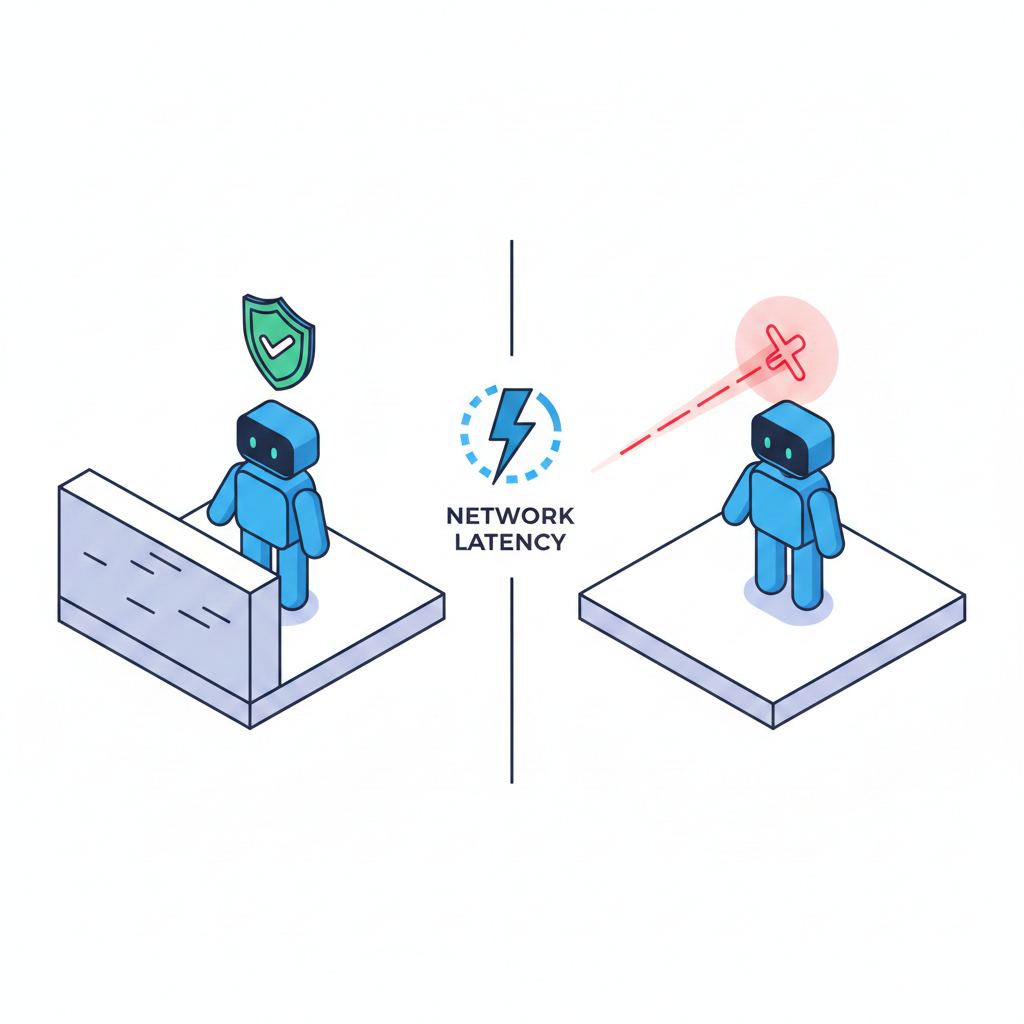
\includegraphics[width=1.0\linewidth]{figures/sec2/image1.png}
    \caption{视图一致性悖论：由于网络延迟（Latency），Client A 与 Client B 在同一物理时刻看到的“真相”截然不同。}
    \label{fig:network-lat}
\end{figure}

其次是\textbf{时序不确定性（Timing Uncertainty）}，指由于网络传输介质的物理特性，导致数据包到达的延迟（Latency）不可预知且次序（Ordering）可能错乱的现象。在单机代码中，函数调用的顺序就是逻辑执行的顺序，因果关系清晰可见。但在网络环境中，网络抖动（Jitter）和丢包（Packet Loss）会无情地打乱这一切。先发出的指令可能后到达，甚至根本不到达。如果服务器简单地按照“收到即执行”的原则处理，那么一场公平的决斗可能会变成比拼谁的网速更快，而不是谁的操作更准。更糟糕的是，如果两个玩家同时操作同一件物品，谁先谁后的判定将直接影响游戏结果。如何在一个异步的、不可靠的网络环境之上，构建一个逻辑上同步、时序上有序的虚拟时间轴，是所有网游后端必须解决的基础难题。

最后，也是最为致命的，是\textbf{信任边界（Trust Boundary）}，即在系统架构中划分出的安全隔离线，用于界定哪些计算节点是可被信任的，哪些是不可信且可能包含恶意行为的。单机游戏中，玩家拥有对自己机器的完全控制权，修改内存数据（如使用“金手指”或修改器）通常被视为个人娱乐行为，不会影响他人。但在竞技网游中，游戏客户端运行在充满恶意的不可控环境里。如果系统盲目信任客户端上报的数据——例如允许客户端直接汇报“我造成了1000点伤害”或“我现在瞬移到了终点”——那么外挂将摧毁整个游戏的公平性基石。玩家可能会通过篡改代码、拦截封包或修改内存来获得不当优势。因此，在线游戏不仅是技术的对抗，更是一场开发者与作弊者之间关于“真相定义权”的攻防战。

更进一步地，这种逻辑困境的普适性远超游戏领域。上述的三大挑战并非游戏所独有，而是所有“多端共享状态的实时在线系统”必须共同面对的工程公理。无论是金融领域中毫秒必争的高频交易系统，还是协同办公软件中多人同时编辑文档的冲突处理，亦或是元宇宙中海量并发的交互同步，其底层逻辑都受制于同样的分布式物理法则。只要系统涉及到多个物理分离的终端对同一个状态进行读写，就必然面临状态谁先谁后（时序）、各端看到的是否一样（视图一致性）以及恶意节点是否篡改数据（信任边界）的问题。多人在线游戏只不过是因为其对高频率交互和低延迟的极端苛刻要求，成为了这些分布式系统难题最集中的“试炼场”。

综上所述，从单机到联机，绝不仅仅是多加一个网络通信模块那么简单。它要求我们将思维模型从“维护一个确定的本地状态”彻底转变为“协调多个不一致的分布式状态”。在本章中，我们将不再把游戏世界视为封闭的本地进程，而是把它进化为一个需要“多终端共同维护”的在线系统。我们将聚焦于三个核心问题：\textbf{谁拥有世界的权威版本}（谁来定义唯一真相）、\textbf{本地视图如何围绕这一真相更新}（输入如何上传、结果如何下发）、以及\textbf{在存在不可信客户端时，哪些逻辑必须被收回到服务器一侧执行}。


% 发展的历史 怎么引入P2P
 
\subsection{初试锋芒：构建直连（P2P）对战原型} % <- 加入Socket编程 给一些代码 

在直面宏大的分布式架构之前，最符合工程师直觉的第一步往往是“奥卡姆剃刀”式的——既然只有两个玩家，为何不直接用一根网线将两台电脑连在一起？这种去中心化的直连模式（Peer-to-Peer, P2P），正是早期局域网联机游戏雏形。为了彻底理解网络同步的机理，我们不妨先动手构建这样一个最小化的 P2P 原型，亲身体验数据是如何跨越物理边界的。

构建这一原型的首要任务是建立通信通道。在操作系统的网络协议栈中，这一过程始于\textbf{套接字（Socket）}的创建。不同于单机程序直接读取内存，网络程序需要向内核申请一个“通信端点”。在双人直连模型中，我们需要人为地指定一方为“主机（Host）”，另一方为“客机（Guest）”。主机启动时会在本地绑定一个端口（Bind）并进入监听状态（Listen），就像是打开大门静候来客；而客机则知晓主机的 IP 地址与端口，主动发起连接请求（Connect）。经过 TCP 的三次握手建立起稳定的全双工通道后，两台物理隔离的计算机便在逻辑上拥有了共享的数据管道。此时，游戏循环（Game Loop）的逻辑发生了本质变化：每一帧的输入不再直接驱动本地逻辑，而是被分流为两路，一路进入本地缓冲区，另一路被序列化为二进制流，顺着网线飞向对手的缓冲区。

构建这一原型的核心挑战在于打破单机环境的封闭性，首要任务即是在操作系统网络协议栈中建立稳定的\textbf{套接字（Socket）}通信通道。网络程序不同于直接寻址内存的本地应用，它必须向内核申请一个逻辑上的通信端点，并通过 \textbf{IP 地址与端口号（Port）}这两大核心要素进行定位。IP 地址如同物理世界的门牌号，负责在复杂的网络拓扑中精确定位对手的计算机；而端口号则像是一座大厦中特定房间的编号，确保数据包能够准确送达对应的原型程序而非其他应用。通过将这两个参数封装进套接字，两台物理隔离的设备便具备了在逻辑层面上“感知”彼此存在的基础。

在具体的实现架构中，系统通过“主机（Host）”与“客机（Guest）”的身份划分来驱动连接。主机通过执行 Bind 操作将套接字与本地特定的端口绑定，随后进入 Listen 状态，在内核层面维持一个静默的监听队列。与此同时，客机携带主机的 IP 地址发起 Connect 请求，通过 TCP 协议标志性的“三次握手”建立起可靠的全双工数据链路。一旦这条逻辑管道贯通，底层游戏循环（Game Loop）的逻辑将发生本质演变：程序不再盲目处理本地输入，而是将每一帧的按键或指令序列化为二进制流，利用建立好的套接字实时外发。这意味着本地逻辑必须等待或预测来自远程缓冲区的数据，两台计算机由此在比特流的交换中达成了状态的同步

在\textbf{Go}语言中，Socket 编程可以通过标准库中的 \texttt{net} 包轻松实现。以下是一个简化的 P2P 连接建立示例：

\begin{tcolorbox}[title=P2P 连接建立示例]
\begin{lstlisting}[style=codeblock, language=go]
ln, err := net.Listen("tcp", "0.0.0.0:8080") // 用户A
conn, err := ln.Accept()
conn, err := net.Dial("tcp", "主机IP:8080") // 用户B
\end{lstlisting}
\end{tcolorbox}

连接建立后，玩家之间的数据交换便可通过读写 Socket 实现。例如，玩家A攻击了玩家B，玩家B的生命值下降了10点，这一信息需要被封装成数据包发送给对手：

\begin{tcolorbox}[title=数据包发送示例]
\begin{lstlisting}[style=codeblock, language=go]
// 发送数据
message := "DAMAGE:10"
conn.Write([]byte(message))
// 接收数据
buffer := make([]byte, 1024)
n, err := conn.Read(buffer)
receivedMessage := string(buffer[:n])
\end{lstlisting}
\end{tcolorbox}
同时，如果玩家B也进行了攻击，类似的消息会被发送回玩家A。通过这种双向的数据流，双方的游戏状态得以在各自的内存中更新。结合前述的游戏循环逻辑，玩家A在本地按下攻击键后，程序会先在本地内存中更新玩家B的生命值，然后将“DAMAGE:10”这一消息通过 Socket 发送给玩家B。给出\textbf{Go}语言的伪代码示例：
\begin{tcolorbox}[title=游戏循环中的数据交换示例]
\begin{lstlisting}[style=codeblock, language=go]
for {
    // 处理本地输入
    input := getLocalInput()
    synchronizeInput(input)
    // 处理接收的数据
    buffer := make([]byte, 1024)
    n, err := conn.Read(buffer)
    processReceivedData(buffer[:n])
}
\end{lstlisting}
\end{tcolorbox}


然而，如果玩家A和玩家B所处的网络环境比较差，导致数据包传输的延迟较高，游戏体验将大打折扣。玩家A在其屏幕上看到自己和玩家B的生命值都仅剩10点，玩家A进行极限操作攻击了玩家B，玩家B的生命值变为0，玩家A赢得比赛。但是玩家B也是在同一时间点看到的自己和玩家A的生命值都仅剩10点，玩家B也进行了极限操作攻击了玩家A，玩家A的生命值变为0，玩家B赢得比赛。最终导致双方都认为自己赢得了比赛，游戏逻辑陷入混乱。

为了保证双方在同一时间点对游戏状态有一致的认知，我们需要引入\textbf{时序同步机制}。在直连模式下，为了保证双方看到的一致性，我们通常采用“帧锁定（Lockstep）”策略。这就好比两个人下棋，必须遵循“你走一步，我走一步”的严格时序。在代码层面，我们将游戏时间切分为一个个离散的“逻辑帧（Turn）”。每一帧开始时，双方必须交换各自的输入指令（如“按下W键”或“点击鼠标”）。
程序会强制等待，直到本地输入和远端输入全部就位，才将这两组输入同时喂给游戏逻辑核心进行演算。
由于计算机的逻辑运算（如果是确定性的）在输入相同的情况下必然产生相同的结果，
只要保证两端收到的输入序列完全一致，两台电脑上的游戏世界就会像精密咬合的齿轮一样同步运转，
无需传输庞大的全量状态数据。

加入帧锁定机制后的伪代码示例如下：
\begin{tcolorbox}[title=帧锁定机制示例]
\begin{lstlisting}[style=codeblock, language=go]
for {
    // 收集本地输入
    localInput := getLocalInput()
    conn.Write([]byte(localInput))

    // 等待接收远端输入
    buffer := make([]byte, 1024)
    n, err := conn.Read(buffer)
    remoteInput := string(buffer[:n])
    // 同步处理输入
    processInputs(localInput, remoteInput)
}
\end{lstlisting}
\end{tcolorbox}
通过这种方式，双方在每一帧都能基于相同的输入序列计算出一致的游戏状态。

当然，我们还希望能保存角色的位置、血量等状态，以便在断线重连时恢复游戏进度，总不能让玩家每次断线都从头开始吧？为了方便起见，我们可以在每次游戏状态更新后，将当前的全量状态序列化并保存到本地文件中。当玩家重新连接时，程序可以读取这个文件，恢复到上次保存的状态，从而实现断线重连功能。

然而，当我们试图将这个看似完美的 P2P 原型搬上广域网时，现实的引力便会将其击碎。
首先是\textbf{流畅度与公平性的博弈}。在帧锁定机制下，游戏的推进速度取决于网络状况最差的那一端，
一旦一方发生网络抖动，另一方的画面也会随之冻结，这种“一人卡顿，全场遭殃”的体验在互联网环境下是致命的。
更严峻的是\textbf{信任危机}。在 P2P 架构中，必定有一方（通常是主机）承载了部分逻辑裁决权，
或者双方各自计算。这就给作弊者留下了巨大的后门：如果玩家 A 修改了本地内存中的判定逻辑（
例如将命中判定范围扩大），玩家 B 的机器要么被迫接受这个错误结果，要么检测到状态不一致导致游戏崩溃（Desync）。

正是这次构建 P2P 原型的尝试，让我们痛切地意识到：在缺乏可信第三方监督、且网络环境不可控的互联网上，
单纯的直连与协商机制极其脆弱。
为了解决“谁说了算”以及“如何不被卡顿拖累”这两个核心痛点，
我们必须打破平等的 P2P 拓扑，引入一个绝对权威的仲裁者。这，便是下一节 CS 架构登场的契机。

\subsection{中流砥柱：CS架构和双人原型} % <- 发展到CS
% <- 一个简单能够接受长连接的S怎么写 -> 轮询
% 现在大家已经知道服务器的特点，那么适用于原型的怎么写呢 并发 并发是两个 
% 同步的锁给个代码 

基于前文分析，虽然P2P架构在《星际争霸1》等早期局域网时代的经典之作中表现优异，凭借“帧同步”与“确定性模拟”实现了低带宽下的高效同步，但这一模式本质上建立在“协作信任”与“高质网络”的假设之上。一旦置身于环境复杂的广域网（WAN），面对网络抖动与人性幽暗，P2P架构便会暴露出其致命的软肋——不仅难以彻底根除作弊，更面临着“一人卡顿，全场等待”的木桶效应。因此，为了构建一个能够适应现代互联网环境、且具备强壮性的双人在线系统，引入一个独立于所有玩家之外的第三方节点，即经典的CS架构（Client-Server Architecture），便成为了必然的进化方向。

\begin{figure}[H]
    \centering
    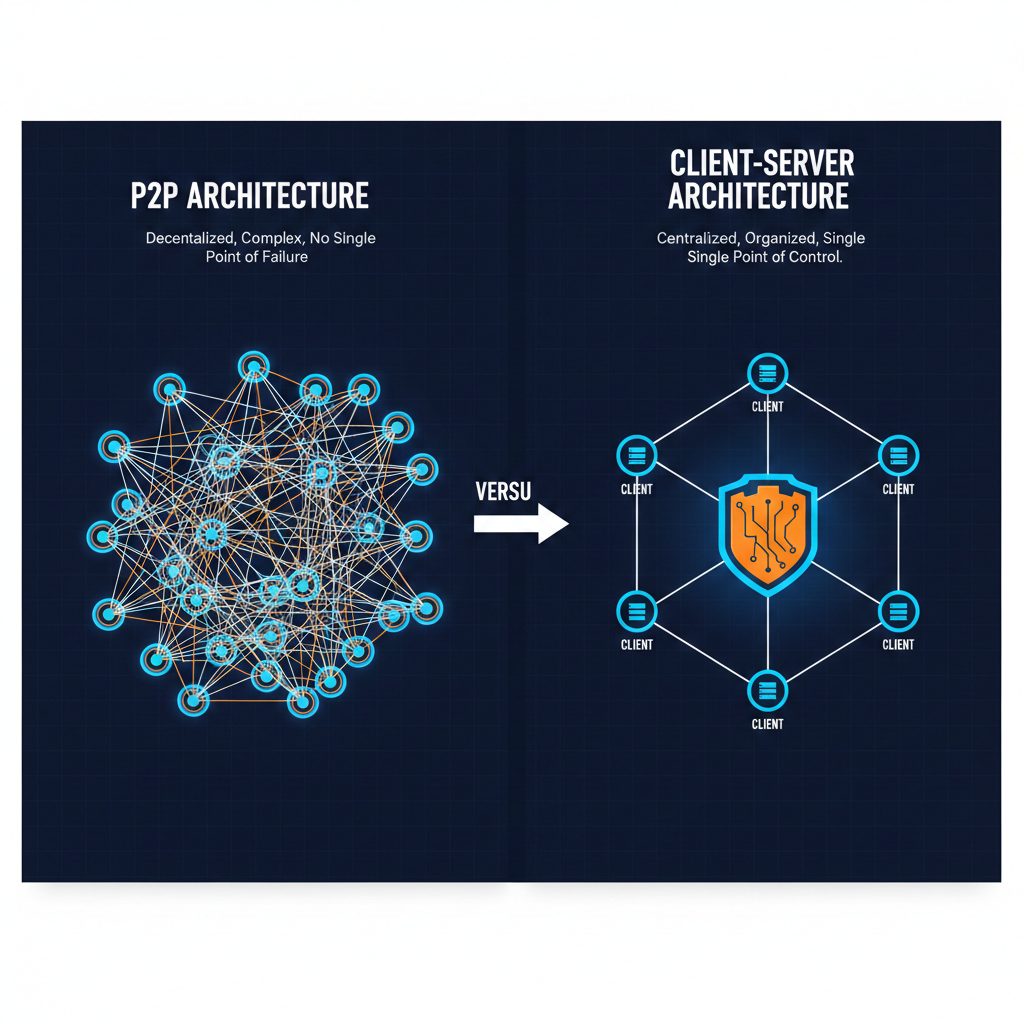
\includegraphics[width=1.0\linewidth]{figures/sec2/image2.png}
    \caption{架构演进：左图为 P2P 全状/网状结构，依赖相互信任；右图为 CS 星型结构，服务器（Server）作为唯一权威节点。}
    \label{fig:p2pvscs}
\end{figure}

在这种架构范式下，核心的变革在于引入了\textbf{权威服务器（Authoritative Server）}这一概念。它绝非仅仅是一个负责转发数据包的中转站，而被定义为\textbf{“游戏世界状态的唯一合法持有者”}。在物理层面，它独立于所有客户端运行；在逻辑层面，它拥有对游戏规则的最高解释权与裁决权。任何客户端计算出的结果——无论是角色的位移、子弹的弹道还是技能的释放——在本质上都仅仅被视为一种“请求”或“本地表现”。唯有经过服务器校验、计算并确认的数据，才是不可篡改的“世界真相”。

我们之所以在本系统中坚定地选择CS架构而非P2P，其深层逻辑在于对\textbf{“信任模型”}的重构。P2P架构更适用于小规模、高频交互且对延迟极度敏感的场景（如局域网联机或格斗游戏），因为它默认参与者之间存在较高的信任度，且网络环境可控。然而，一旦游戏场景涉及强对抗性（Anti-cheat）、持久化资产（如经济系统或装备存档）或是大规模连接，客户端便不再可信。此时，CS架构通过“零信任”原则，强制将计算权收归服务端，虽然这不可避免地牺牲了部分响应速度（RTT），但却换取了整个系统的安全性与一致性。简而言之，当游戏从“协作体验”转向“竞争博弈”时，架构必须从P2P的“多方共识”转向CS的“独裁仲裁”。

这种权力的转移，直接导致了客户端角色的\textbf{降维}与输入模式的\textbf{重构}。在CS架构中，客户端从全知全能的“主宰”退化为了一个高级的“哑终端”。它不再负责核心逻辑的推演，而是专注于交互意图的采集与画面的渲染表现——即“逻辑与表现的分离”。当玩家按下键盘上的“W”键时，客户端无权直接修改角色的坐标，它只能将这个“移动意图”封装成数据包发送给服务器。此时屏幕上的角色移动，在逻辑上仅仅是对服务器未来状态的一种“预测”或对已确认状态的“回放”。

这一机制的优越性，将在我们即将构建的双人追逐战原型中得到淋漓尽致的体现。设想若没有权威服务器，当玩家A声称抓住了玩家B，而B声称已逃脱时，系统将陷入无解的罗生门。而在权威服务器模式下，流程被重塑为：玩家A上传“攻击操作”；服务器基于内存中维护的权威坐标进行距离校验与逻辑运算；若判定有效，服务器更新状态并广播结果。此时，即便玩家B试图通过本地外挂锁定血量，或者因网络延迟看到了错误的位置，一旦收到服务器下发的权威快照，他的客户端必须无条件地执行状态回滚（Reconciliation），修正本地数据以符合服务器的裁决。这便是“权威性”的核心价值所在。

为了验证这一理论，我们将摒弃商业引擎的图形干扰，从零构建一个“双人原型”。
在这个原型中，服务器将是一个运行在控制台的纯逻辑进程，它看不见任何图形，只处理坐标数值、状态枚举与伤害公式；
而客户端则负责将玩家操作转化为网络流，并将服务器下发的抽象数据流转化为屏幕上的红蓝方块。

首先我们将前文的伪代码结构进行调整，以适应CS架构的需求：
\begin{tcolorbox}[title=CS架构伪代码结构,label=code:cs_structure]
\begin{lstlisting}[style=codeblock, language=go]
for {// 服务器端主循环
    // 接收客户端输入
    inputA := receiveInputFromClientA()
    inputB := receiveInputFromClientB()
    // 处理游戏逻辑
    updateGameState(inputA, inputB)
    // 广播权威状态
    broadcastState()
}
for { // 客户端主循环
    // 采集本地输入
    localInput := getLocalInput()
    sendInputToServer(localInput)
    // 接收权威状态
    gameState := receiveGameStateFromServer()
    renderGameState(gameState)
}
\end{lstlisting}
\end{tcolorbox}

从上面的结构可以看出，服务器端的主循环负责接收来自两个客户端的输入，处理游戏逻辑，
并将更新后的权威状态广播回各个客户端；而客户端则专注于采集本地输入、发送给服务器，
并渲染服务器下发的权威状态。这就可以确保所有玩家可以看到一致的游戏世界，解决了前文提到的\textbf{视图一致性}问题。



\subsection{运筹帷幄：连接管理、状态仲裁以及世界同步}

在确立了以服务器为中心的架构范式后，我们需要透过宏观的拓扑结构，深入拆解服务器内部微观的运作机理。
一个成熟的后端系统，绝非仅仅是一个被动接收并转发比特流的数据中转站，而应当是一个拥有高度自主权、
时刻处于高速逻辑运算中的“大脑”。

在我们的双人对战原型乃至更复杂的分布式系统中，这个“大脑”的运转逻辑被严谨地解构为三个相互依存的核心模块：
\textbf{连接管理（Connection Management）}、\textbf{状态仲裁（State Arbitration）} 以及 
\textbf{世界同步（World Synchronization）}。这三者分别对应了分布式计算中的资源生命周期维护、
数据一致性保障以及状态分发机制，共同构成了在线业务后端的最小完备闭环。


\begin{figure}[H]
    \centering
    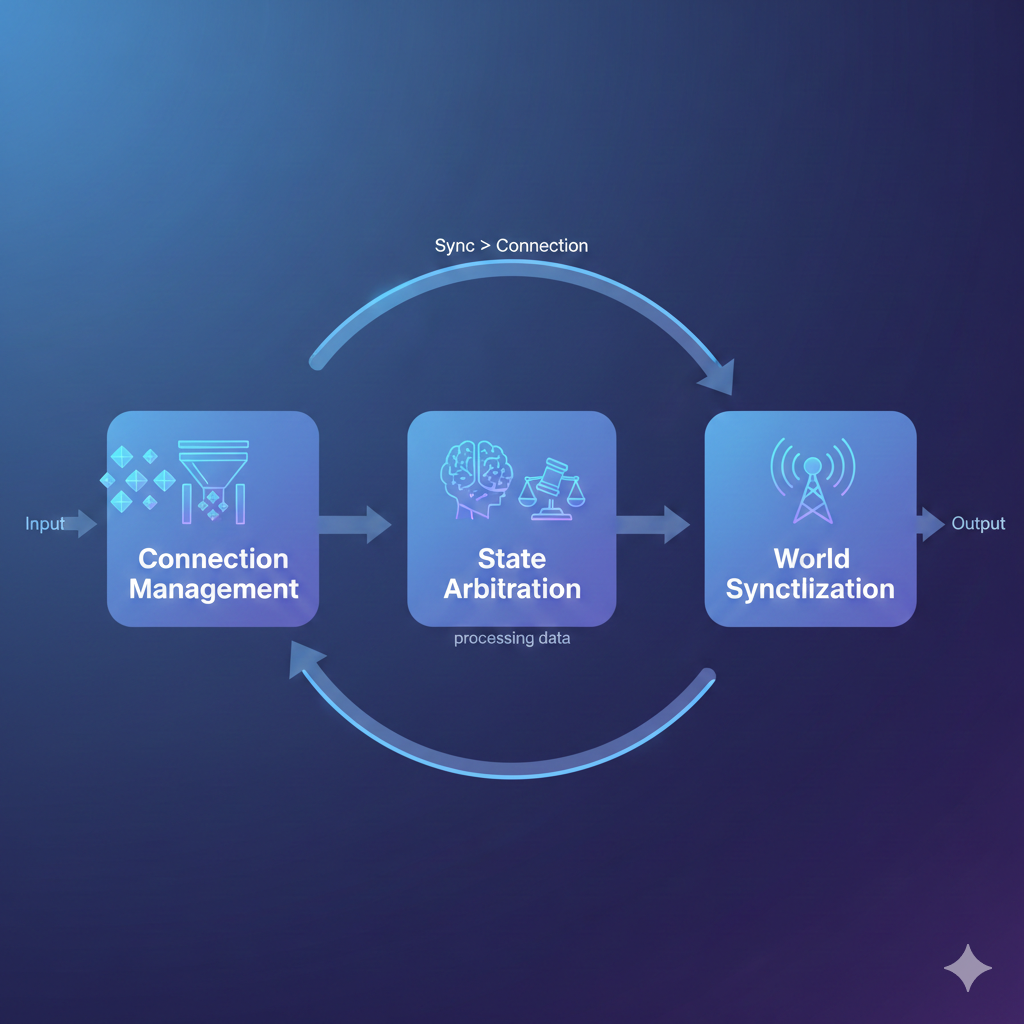
\includegraphics[width=1.0\linewidth]{figures/sec2/image3.png}
    \caption{服务器逻辑闭环：数据经由“连接管理”流入，在“状态仲裁”层进行逻辑校验与更新，最终通过“世界同步”广播回客户端。}
    \label{fig:csmodules}
\end{figure}
\subsubsection{连接管理：会话的生命周期守护与资源调度}

连接管理是任何长连接服务的门户与基石。在通用的分布式系统语境下，它的核心职责在于\textbf{“资源的动态分配与上下文维护”}。无论是即时通讯软件、金融交易终端还是网络游戏，服务器必须在不可靠的物理网络之上，抽象出一个可靠的逻辑会话层，以确保每一个接入终端都能被精确地标识、追踪与管理。

在游戏服务器的具体实现中，连接管理的角色远超底层的 TCP Socket 握手。它首先承担着“守门人”的重任，负责在传输层之上构建应用层的准入机制。当客户端发起连接请求时，管理模块必须执行严格的合法性校验（例如 Token 验证或加密握手），以过滤掉无效的扫描流量或恶意的 DDoS 攻击尝试。

一旦连接建立，服务器随即进入资源调配阶段，为该客户端分配全局唯一的会话 ID（Session ID），并在内存堆中开辟一块专用的上下文区域（Context）。这块区域不仅存储着玩家的网络句柄，还承载着序列号管理、拥塞控制窗口以及断线重连所需的快照数据。

更为关键的是，连接管理模块必须具备极高的鲁棒性来应对移动网络环境的波动。它通过精密的\textbf{心跳检测机制（Heartbeat）}与\textbf{超时策略}，敏锐地量化连接的健康度，从而区分正常的“用户静默”与异常的“网络掉线”。针对游戏场景中常见的网络抖动，成熟的管理模块不会在检测到断开的瞬间立即销毁数据，而是通过引入“会话保持期（Session Persistence）”或“影子状态”，允许客户端在特定时间窗口内通过重连协议无缝恢复上下文。这种设计既避免了因网络瞬断导致的频繁登出，也确保了在用户彻底离开时能通过回调机制优雅地释放内存，防止因“僵尸连接”堆积而引发生的资源泄露危机。

在完善了基础网络框架后，我们需要对 \ref{code:cs_structure} 中的输入处理逻辑进行升级。
为了解决裸连接（Raw Connection）难以维护状态的问题，我们引入 clientConn 结构体。
它将底层的网络连接与玩家的业务属性（如会话 ID、心跳时间、事件队列）封装在一起，实现标准化的连接管理。

\begin{tcolorbox}[title=连接管理的结构体定义] 
\begin{lstlisting}[style=codeblock, language=go]
type clientConn struct { 
    id int // 唯一会话标识 
    Conn net.Conn // 底层 TCP/UDP 连接 
    lastHeartbeat time.Time // 最后心跳时间，用于超时检测 
    EventQueue chan InputEvent // 输入事件缓冲通道 
}
// 实例化客户端连接对象 
var clientA clientConn 
var clientB clientConn
\end{lstlisting} 
\end{tcolorbox}

然后我们会使用上面定义过的结构体，来处理并管理请求。


\begin{tcolorbox}[title=连接管理伪代码示例]
\begin{lstlisting}[style=codeblock, language=go]
func handleConn(client *ClientConnection) {
    for { // 读取数据
        input, err := receiveInputFromClient(client.Conn)
        if err != nil { // 处理断线或错误
            handleDisconnect(client)
            return
        }
        client.LastHeartbeat = time.Now() // 更新心跳时间
        client.EventQueue <- input  // 将输入放入事件队列
    }
}
go handleClientConnection(&clientA)
go handleClientConnection(&clientB)
tiker := time.NewTicker(tikeoutDuration)
for { // 从事件队列中获取输入
    select {
    case <- tiker.C: // 检测超时
        checkAndHandleTimeout(&clientA)
        checkAndHandleTimeout(&clientB)
    }
    updateGameState()  // 处理游戏逻辑
    broadcastGameStateToClients() // 广播权威状态
}
\end{lstlisting}
\end{tcolorbox}

此时，连接管理模块已经能够高效地维护每个客户端的会话状态，整个游戏的进程不会因为单个连接的波动而受到影响。
并且，通过划分每帧的输入处理与超时检测，我们在一定程度上缓解了网络抖动对游戏体验的冲击，解决了\textbf{时序不确定性}的问题。


\subsubsection{状态仲裁：逻辑的一致性防线与真理裁决}

状态仲裁是服务器架构中“权威性（Authority）”的集中体现。在广泛的软件工程领域，这对应着\textbf{“单一数据源（Single Source of Truth）”}与\textbf{“业务逻辑校验”}的核心原则。在一个互不信任的客户端-服务器网络环境中，永远不能假设接入端的输入是诚实或正确的，因此服务器必须作为唯一的真理裁决者，对所有状态变更请求进行审计与执行。

在激烈的双人对战中，每秒钟可能会有海量的操作指令——从移动向量到技能触发——如潮水般涌向服务器。仲裁模块决不会盲目地根据客户端的指令更新状态，而是构建了一套严密的\textbf{“先校验，后执行”}的流水线体系。

以空间位置更新为例，当服务器接收到移动请求时，并不会直接采信客户端上报的目标坐标，
而是引入物理引擎或碰撞检测算法进行逻辑复核：系统会根据上一帧的权威位置、
时间差以及角色的最大理论速度，计算出合理的移动包络线。只有当请求落在这个合法范围内，
且未穿越不可逾越的地理屏障（NavMesh）时，该操作才会被标记为有效。同理，在处理战斗交互时，
仲裁模块会完全忽略客户端上报的“命中结果”，转而依据服务器端记录的时间切片和空间状态，
重新进行一次权威的判定。通过这种严苛的过滤机制，服务器彻底杜绝了诸如加速、穿墙或篡改数据等作弊行为，
确保了所有参与者都在同一套不可被逾越的规则下进行公平竞技。

为了将状态仲裁的逻辑融入到 \ref{code:cs_structure} 中的游戏逻辑处理部分，我们可以修改如下：
\begin{tcolorbox}[title=状态仲裁伪代码示例]
\begin{lstlisting}[style=codeblock, language=go]
func processInputFromClientA(input InputEvent) {
    // 校验输入合法性
    if isValidInput(input, playerA.State) {
        // 更新玩家A状态
        updatePlayerState(&playerA, input)
    } else {
        log.Println("Invalid input from Client A:", input)
    }
}
func processInputFromClientB(input InputEvent) {
    // 校验输入合法性
    if isValidInput(input, playerB.State) {
        // 更新玩家B状态
        updatePlayerState(&playerB, input)
    } else {
        log.Println("Invalid input from Client B:", input)
    }
}
\end{lstlisting}
\end{tcolorbox}

此时，状态仲裁模块已经能够有效地过滤掉异常或恶意的输入请求，确保游戏逻辑的纯净性与一致性，解决了\textbf{信任边界}的问题。

然而，仅有仲裁还不够——服务器内存中的权威状态是易失的。一旦服务器进程重启或玩家断线，内存中的角色坐标、生命值等数据将随之消失。如果每次断线都让玩家从零开始，游戏体验将无从谈起。因此，我们需要在状态仲裁的基础上引入持久化机制，将关键的玩家状态定期写入磁盘存储。

持久化的位置选择同样遵循信任边界原则。如果将存档保存在客户端本地，玩家可以轻易篡改存档文件来伪造属性；而将存档保存在服务器端的数据库中，则能确保数据的权威性与完整性。在我们的双人原型中，选择SQLite作为轻量级的嵌入式数据库——它无需独立的数据库服务进程，只需一个本地文件即可运行，非常适合教学原型的快速验证。

具体而言，我们定义一个存储接口，将玩家的核心状态（名称、坐标、生命值）抽象为可持久化的记录：

\begin{tcolorbox}[title=持久化存储接口]
\begin{lstlisting}[style=codeblock, language=go]
type StoredPlayer struct {
    Name string
    X, Y int
    HP   int
}

type Store interface {
    LoadPlayer(name string) (*StoredPlayer, error)
    SavePlayer(p StoredPlayer) error
}
\end{lstlisting}
\end{tcolorbox}

每当状态仲裁模块完成一次合法的状态变更（如移动校验通过、战斗结算完毕），服务器便调用\texttt{SavePlayer}将最新状态写入数据库。这里采用``INSERT ... ON CONFLICT DO UPDATE''（即UPSERT）语义，确保无论玩家是首次登录还是已有存档，都能用一条语句完成写入。当玩家断线后重新连接时，服务器在注册阶段调用\texttt{LoadPlayer}，若数据库中存在该玩家的记录，则以存档数据恢复其坐标与生命值，而非重新随机生成。

需要指出的是，当前原型在每次状态变更后都立即执行数据库写入，这种同步持久化方式在双人场景下完全可行，但在高并发场景下会因频繁的磁盘I/O成为性能瓶颈。第三章将引入Redis内存缓存与异步写回策略来解决这一问题。
\subsubsection{世界同步：状态的最终一致性与高效分发}

世界同步模块负责闭合信息流动的环路，将服务器内部经过仲裁的权威结果反馈给所有参与者。在分布式计算理论中，这属于\textbf{“状态复制（State Replication）”}与\textbf{“发布/订阅（Pub/Sub）”}模式的范畴。其核心挑战在于如何在有限的网络带宽与高频的实时性要求之间找到平衡点，以实现系统状态的\textbf{“最终一致性”}。

服务器维护的真理如果仅停留在内存中，对于玩家而言便是毫无意义的黑盒。因此，同步模块需要以固定的高频率（即 Tick Rate，如 30Hz 或 60Hz）驱动整个世界的演变，并将每一帧内的状态变更——包括位置迁移、属性增减、动画状态切换等——转化为数据流广播出去。

这一过程不仅是数据的搬运，更是复杂的工程权衡艺术。为了避免全量数据广播带来的带宽风暴，现代同步模块广泛采用\textbf{“增量同步（Delta Synchronization）”}与\textbf{“快照（Snapshot）”}相结合的混合策略。对于初次进入视野的实体，系统发送包含完整状态的全量快照；而对于已存在于上下文中的实体，则仅发送自上一帧以来发生变化的属性差值。此外，为了进一步压榨传输效率，还需要引入 Protocol Buffers 或 FlatBuffers 等高效序列化技术，将结构化对象压缩为紧凑的二进制流。当客户端接收到这些权威数据包后，结合本地的插值（Interpolation）与预测（Prediction）算法，便能平滑地渲染出连续的画面，从而在玩家的感官层面构建出一个与对手实时互动、毫无违和感的统一时空。

为了将世界同步的逻辑融入到 \ref{code:cs_structure} 中的广播权威状态部分，我们可以修改如下：
\begin{tcolorbox}[title=世界同步伪代码示例]
\begin{lstlisting}[style=codeblock, language=go]
func broadcastGameStateToClients() {
    // 构建增量状态包
    deltaStateA := constructDeltaState(playerA, lastSentStateA)
    deltaStateB := constructDeltaState(playerB, lastSentStateB)
    // 发送给客户端A
    sendGameStateToClient(clientA.Conn, deltaStateA)
    // 发送给客户端B
    sendGameStateToClient(clientB.Conn, deltaStateB)
    // 更新上次发送状态
    lastSentStateA = playerA.State
    lastSentStateB = playerB.State
}
\end{lstlisting}
\end{tcolorbox}

\subsubsection{合璧成环：三模块的协同闭环}

通过上述三个模块的精密咬合——连接管理维持通信通道的稳定性，状态仲裁确立逻辑事实的唯一性，世界同步保障感知层面的实时性——我们的双人对战原型便拥有了完整的生命力。这一架构不仅解决了基础的联机互通需求，更在底层设计上预置了针对网络延迟（Latency）的容错能力与针对恶意行为（Cheating）的免疫能力，为后续章节中探讨大规模并发（Concurrency）与更复杂的战斗逻辑奠定了坚不可摧的标准范式。

%%

\subsection{狭路相逢：双人对战流程全景}


在前两节的论述中，我们分别从系统架构的宏观视角和模块职责的微观维度，详细阐述了双人在线原型的设计思路：服务器作为绝对的权威仲裁者，全权负责网络连接管理、全局状态仲裁以及世界状态的同步；而客户端则专注于用户输入的实时采集与游戏画面的渲染展示。为了更具体地展示这一架构在实际运行中的动态表现，本节将打破静态的模块划分，沿着一场标准对战的时间轴线，从玩家相遇、交互发起到胜负裁决的完整生命周期，从全链路的整体视角深度梳理前述机制是如何协同工作的。这不仅是对功能的串联，更是对“权威服务器”设计模式在时序逻辑上的具体印证。

\subsubsection{对战前阶段：相遇与可见性建立}

在对战尚未触发的自由探索阶段，服务器不仅维护着所有在线玩家的坐标数据，更在每一个逻辑帧中基于权威坐标执行严格的空间查询与可见性计算。系统会根据预设的感兴趣区域（AOI, Area of Interest）算法，动态判断实体间的拓扑关系。对于任意一对玩家，当其中一方的坐标进入另一方的视野半径时，服务器会首先在内存中更新双方的视野列表（View List），随后在接下来的状态同步周期中，将这一新增的实体信息序列化并打包进下行数据包。

客户端在接收到数据包并反序列化后，会在本地场景图中实例化对应的角色模型，玩家侧由此感知到“地图上出现了一名新对手”。在此过程中，必须强调的是，所有的可见性判断——即“谁能看见谁”——完全由服务器基于其内存中的权威状态独立完成。客户端仅作为被动的接收端，负责将服务器下发的逻辑状态“翻译”为视觉图像。这种单向的数据流设计，确保了在网络波动或客户端被篡改的情况下，全局的可见性关系依然保持逻辑上的严密统一，彻底杜绝了客户端预判导致的“幽灵玩家”或视野状态不同步的割裂现象。

\subsubsection{对战发起：资格判定与会话原子性}

当玩家之间建立了可见关系后，系统并未立即进入战斗状态，而是需要进行更细粒度的条件校验。随着两名玩家的距离进一步缩短并触及预设的交战阈值，服务器会在内存状态机中将双方标记为“潜在可交互”状态，并通过轻量级的状态位更新通知客户端。客户端 UI 层据此激活交互控件，向玩家展示“可以发起对战”的视觉提示。此时，尽管界面上允许操作，但这一提示仅代表一种客户端的本地预测，并未对服务器端的逻辑状态产生任何实质性变更。

一旦某位玩家触发对战请求，客户端会将该操作意图编码为特定的请求消息（Request）发送至服务器。服务器在接收到该请求后，绝不会盲目响应，而是基于当前这一帧的最新权威数据进行一次严格的原子性校验：重新计算双方距离是否仍在合法范围内、确认双方是否仍处于空闲状态、以及检查是否涉及第三方冲突。这一过程类似于数据库事务的隔离性检查，只有当所有前置条件在当前逻辑帧内同时满足时，服务器才会通过校验，在内存中实例化一个对战会话（Session）对象，并将两名玩家的状态机从“自由移动”原子性地切换至“对战锁定”。随后的状态同步将这一确定性的状态变更广播回客户端，从而将界面上的操作意图转化为服务器端受管理的正式会话。

\subsubsection{战斗过程：确定性裁决与逻辑投影}

为了最大限度地凸显服务器端权威判定的核心价值，本书有意选取了一种极简的单回合对战模型作为首个原型，暂时剥离了复杂的技能树与即时演算系统。在这一高抽象度的模型中，战斗过程本质上是一次由服务器主导的确定性计算：在特定的逻辑帧上，服务器锁定双方状态，读取关键属性，依据统一算法产出唯一结果，并写入权威数据。

具体而言，当流程进入裁决阶段，服务器会从持久化层或内存缓存中调取两名玩家的基础战力、当前生命值及所有生效的增益状态。原型实现采用了一套标准的数值对抗公式——例如以战力差值为基准，引入受控的伪随机数序列作为扰动因子——从而计算出不可辩驳的胜负判定。紧接着，服务器在同一逻辑线程内执行状态更新（State Update）：胜方获得经验积累，败方扣除生命值。整个过程是一个严格的黑盒计算，完全不依赖客户端的任何输入或本地运算结果。即便恶意客户端通过内存修改在本地伪造了“暴击”或“闪避”的视觉效果，由于这些数据从未参与服务器端的逻辑运算，因此无法对最终的权威裁决产生丝毫影响。这一设计贯彻了网络游戏开发的核心铁律：客户端仅负责请求的发起与结果的视觉投影，而所有涉及游戏性（Gameplay）的逻辑演算必须在权威服务器的安全边界内闭环。

\subsubsection{对战结算：状态一致性与分布式事务}

当胜负结果被写入权威状态后，系统进入生命周期的最后阶段：结算同步与世界状态回退。这一过程在逻辑上等同于一次分布式事务的提交与连接释放。首先，服务器构建包含胜负判定、属性变更增量及后续状态指令的结算数据包，并下发给相关客户端。客户端解析后，驱动 UI 弹出结算面板并播放相应的胜负动画。需要注意的是，客户端展示的数值变化完全是服务器数据的副本，客户端本地绝不执行任何属性的加减运算。

与此同时，服务器执行逻辑状态的回退操作（Rollback），将两名玩家从独占的“对战会话”中解耦，并在同一逻辑帧内将他们的状态机重置为“自由移动”模式，重新纳入常规的大世界同步循环。在随后的广播周期中，周围的其他玩家将基于新的全局状态，观察到这两名角色结束了战斗状态或发生了位置变更。至此，一个包含相遇检测、会话建立、逻辑裁决及状态重置的完整闭环在服务器端严丝合缝地执行完毕，并在客户端侧呈现为一段连贯流畅的游戏体验。

\subsubsection{从游戏到分布式系统：本质的统一}

跳出具体的游戏场景，若我们将视角上升至分布式系统架构的高度，会发现上述的双人对战流程本质上是一个典型的 \textbf{状态机复制（State Machine Replication）} 与 \textbf{中心化一致性（Centralized Consistency）} 问题的工程实践。

在这个模型中，服务器扮演着 Leader 或 Coordinator 的角色，维护着系统的单一真值（Source of Truth）；而所有的客户端则是分布在不同网络节点的 Follower 或 Replica。玩家的操作不再仅仅是游戏指令，而是向协调者发起的远程过程调用（RPC）或事务请求。服务器对“相遇”的判定对应着分布式系统中的邻居发现与拓扑维护；“对战发起”时的资格校验，实则是为了防止竞态条件（Race Condition）而设置的分布式锁或乐观并发控制；而“战斗裁决”则是事务的具体执行逻辑，确保了在不可靠的网络环境下，系统状态（如玩家血量、积分）变更的原子性（Atomicity）与一致性（Consistency）。通过这种架构，我们解决的不仅仅是游戏玩法的同步，更是如何在存在网络延迟和不可信节点的分布式环境中，保证系统全局状态有序演进这一核心计算机科学难题。

\subsubsection{流程总结}

为了更直观地理解这一涵盖了网络通信、逻辑运算与状态管理的复杂交互过程，我们将上述从相遇、就绪、裁决到结算的完整时序绘制成图~\ref{fig:battle_flow}。从图中可以清晰地看到，客户端与服务器被网络边界严格隔开：尽管客户端承载了复杂的画面表现和用户交互，但所有跨越网络边界的关键指令——无论是视野的判定（Visibility）、状态的流转（State Transition）还是胜负的产生（Arbitration）——其逻辑闭环始终收敛在权威服务器内部，客户端仅仅是这一权威逻辑的“投影仪”。

\begin{figure}[htbp]
    \centering
    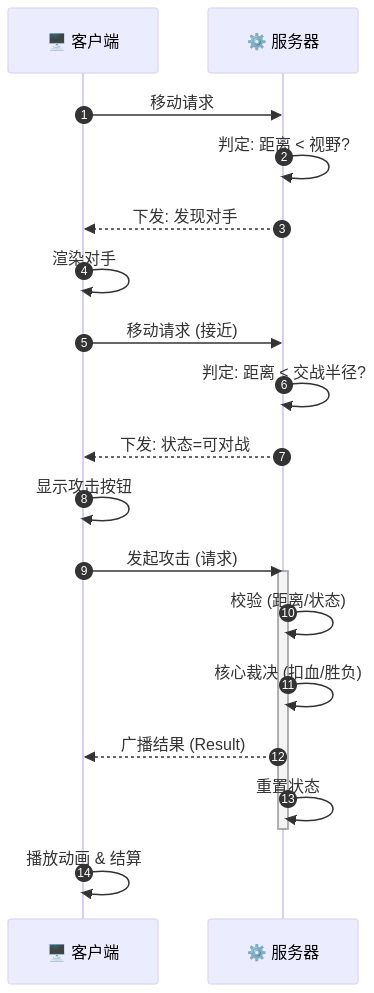
\includegraphics[width=0.45\linewidth,keepaspectratio]{figures/battle_flow.png}
    \caption{整体流程}
    \label{fig:battle_flow}
\end{figure}

回顾本章开头提出的三类挑战，可以看到：视图一致性通过服务器统一维护可见关系与世界同步来保障；时间与顺序问题通过集中化的请求校验和单线程裁决来化解；而信任边界则通过将关键逻辑彻底收拢到服务器一侧而得到收紧。本节给出的双人对战流程，为后续在并发规模和地图数量进一步扩展时的系统演化，提供了一个清晰可依的基本形态。

\subsection{小结：双人原型的确立与并发时代的前夜}

至此，我们不仅完成了一个双人对战原型的构建，更重要的是确立了网络游戏开发中至关重要的认知里程碑：构建在线世界的核心，在于搭建由\textbf{连接管理}、\textbf{逻辑仲裁}以及\textbf{状态同步}所构成的最小闭环。在这个闭环中，我们剥离了单机时代的思维惯性，确立了一条不可逾越的铁律——服务器是唯一的权威熵源，它只负责产出不可辩驳的\textbf{结果}；而客户端则退化为表现层，它只负责上报玩家的\textbf{意图}并如实呈现服务器下发的结论。这种“意图上报”与“结果下发”的异步循环，正是所有多人在线交互系统的基石。

回顾本章历程，我们正是基于上述理论，完成了从单机思维向在线思维的第一次系统性跨越。在单机模式下，世界被封闭在本地进程的孤岛中，内存状态即是真理；而一旦引入网络，多端数据的不一致性迫使我们必须划定明确的信任边界。为此，我们引入了经典的 CS (Client-Server) 架构作为解决方案：将服务器定义为无渲染的纯逻辑实体，它在内存中维护着唯一的“世界真相”。通过双人对战这一具象场景，我们演示了服务器如何作为连接中介管理会话，如何作为状态管理者收敛数据，以及如何作为逻辑仲裁者处理移动与攻击指令。在这个体系下，任何本地计算都仅仅是对未来的预测，只有服务器的裁决才是最终的历史。

然而，从工程演进的视角审视，目前的成果依然是一个“教学友好”的温室模型。我们的世界目前仅容纳两名玩家，且服务器逻辑严格遵循单线程的时间线顺序执行。在微观的低负载环境下，这种简单的请求-响应模型足以维持世界的运转；但一旦我们将视野投向宏观的真实环境——当成百上千名玩家挤入同一张地图，海量的登录、移动与战斗请求将如洪水般涌入单一的逻辑通道。

此时，简单的顺序处理将瞬间成为性能的瓶颈，任何微小的阻塞都会被放大为全局的停滞。更严峻的是，当多名玩家同时争抢同一份资源或修改同一组数据时，缺乏并发控制的系统极易陷入数据竞争与状态错乱的深渊。因此，接下来的第三章将是工程实践的又一次飞跃。我们将引入 Go 语言强大的并发原语 (Goroutine)，打破顺序执行的枷锁，让服务器具备同时处理成千上万个并发连接的能力；同时，我们将引入锁与同步机制来应对高并发带来的复杂性挑战。如果说本章解决了“为什么需要服务器”的定性问题，那么下一章将致力于解决“如何让服务器在洪峰压力下依然稳如磐石”的定量难题。

\newpage    
\section{第三章\ 英雄集结：让世界容纳千军万马} 
% 谢先衍 接第二章的尾 把问题重述一遍 然后解释一下

第二章完成了从单机思维到在线思维的范式迁移：我们建立了以权威服务器为核心的CS架构，通过连接管理、状态仲裁与世界同步三大模块，实现了双人对战的稳定运行。这一原型验证了"服务器作为唯一真相源"的正确性，也为后续扩展奠定了可验证的基线。

然而，当我们尝试将这个双人原型扩展为"多人同图"时，会立即遭遇新的系统瓶颈。这不是玩法设计的问题，而是计算资源组织方式的根本性挑战。当地图中同时存在数十乃至上百名玩家时，每秒产生的状态更新事件、位置同步请求、战斗判定计算将呈指数级增长。如果服务器仍然采用"顺序处理每个请求"的朴素模式，响应延迟会迅速恶化，最终导致玩家体验崩塌。

本章的核心命题是：在单机资源边界内，如何通过并发模型与性能优化，将服务器从"能跑双人"提升到"稳定承载多人同图"。这一阶段对应云计算能力曲线中的纵向优化阶段——在进行分布式横向扩展之前，必须先把单机潜力压榨到极致，建立可观测的性能基线，从而判断何时应该继续优化、何时必须转向分布式架构。我们将从并发模型的建立、共享数据的安全保护，以及资源池化与数据分层三个维度，系统性地解决单机服务器在高并发场景下的核心约束。

% \subsection{万人集结：并发的奥秘} 
\subsection{万人集结：并发的系统必然性}
% 什么是并发
% 协程需要介绍一下 与线程 进程的区别 并发在goroutine中的体现 -> 协程
% 
% \paragraph{本节目标}  理解并发本质，掌握 Go 的 goroutine+Channel 逻辑。

\subsubsection{多人同图下的系统瓶颈}

在第二章的双人原型中，服务器的处理逻辑相对简单：接收玩家A的移动请求，验证其合法性，更新状态后广播给玩家B；接着以相同流程处理玩家B的请求。由于只有两个连接、有限的事件密度，顺序执行模式完全可以满足实时性要求。然而，当我们将场景扩展到"50人同图"时，系统负载特征发生质变，暴露出顺序执行模型在高并发场景下的四大核心瓶颈。

\begin{figure}[H]
    \centering
    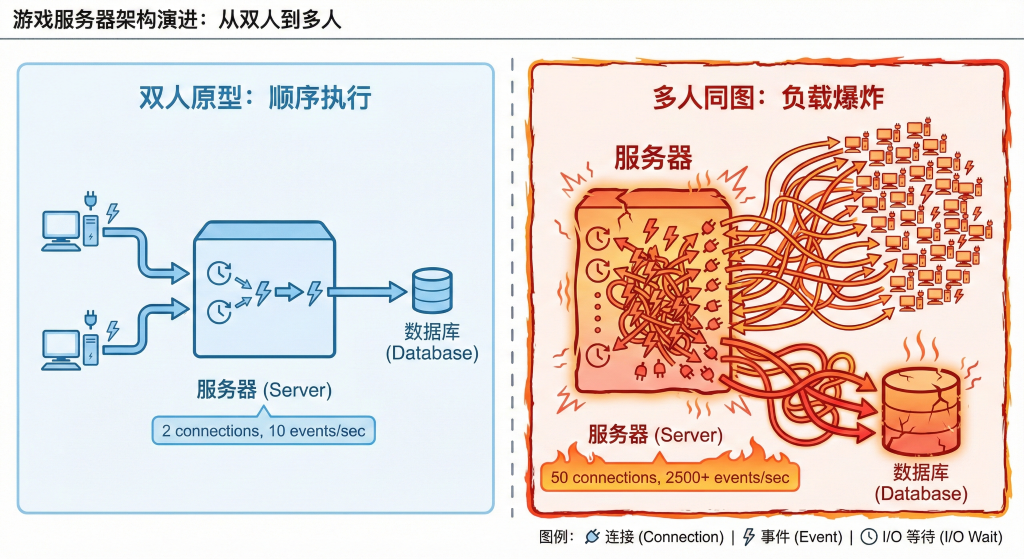
\includegraphics[width=1.0\linewidth]{figures/sec3/image3-1.png}
    \caption{从双人原型到多人同图的系统负载变化：连接数、事件密度和I/O等待的指数级增长}
    \label{fig:concurrent-load}
\end{figure}

第一个瓶颈是连接规模的爆炸性增长。系统需要维护的WebSocket长连接数从2个增长到50个，而每个连接都需要独立的读写缓冲区、心跳检测机制与超时管理逻辑。如果采用传统的"一个操作系统线程处理一个连接"模型，每个线程需要预分配约1到8MB的栈空间，50个连接就可能消耗数百MB内存。更严重的是，操作系统线程的创建和销毁涉及系统调用，上下文切换需要保存和恢复完整的CPU寄存器状态，这些开销在高频场景下会成为显著的性能拖累。当连接数增长到数百、数千时，传统线程模型将因内存耗尽和调度开销过大而崩溃。

第二个瓶颈是事件密度的指数级放大。假设每名玩家平均每秒发送5次操作（包括移动、攻击、技能释放等），服务器就需要处理250次每秒的输入事件。但这只是输入侧的负载，输出侧的压力更为严峻。每次状态变更都需要广播给视野内的其他玩家，假设平均每人视野内有10名玩家，则每秒需要发送2500次状态同步消息。这种广播放大效应使得网络带宽消耗和消息序列化开销呈平方级增长。在顺序执行模型中，处理这些事件的总时间是所有单次操作时间的简单累加，当事件密度超过处理能力上限时，消息队列会迅速积压，响应延迟从毫秒级恶化到秒级。

第三个瓶颈是I/O等待时间的全局传播。在单机服务器中，许多操作都涉及I/O等待：从Redis读取玩家位置需要等待网络往返，从PostgreSQL查询装备信息需要等待磁盘读取，向客户端发送消息需要等待TCP缓冲区就绪。在顺序执行模型中，主线程在等待玩家A的数据库响应时会完全阻塞，无法处理其他玩家的请求。这意味着一个玩家的数据库延迟会传播到所有其他玩家，造成全局性的响应延迟增长。即使系统配备了高性能CPU和大容量内存，这些计算资源也会因为I/O等待而长时间处于空闲状态，资源利用率极低。

第四个瓶颈是共享资源的并发访问冲突。当多个玩家几乎同时操作同一资源（如拾取地图上唯一的宝箱、攻击同一个Boss、占领同一个据点）时，系统必须确保操作的原子性和结果的确定性。在单线程模型中，这个问题被天然规避了——所有操作按照到达顺序依次执行，不存在并发冲突。但一旦引入并发处理，如果没有合理的同步机制，就可能出现"两人都认为自己拾取成功"的数据竞争，破坏游戏规则的公平性和确定性。这类问题的根源在于检查和修改操作之间存在时间窗口，多个执行流可能同时通过检查条件并执行修改操作。

这四大瓶颈不是网络游戏特有的现象，而是所有高并发在线服务在单机阶段必然遭遇的通用约束。无论是即时通讯系统、金融交易平台，还是协同办公应用，只要系统需要同时服务大量并发用户，就会面临相同的资源组织挑战：多路连接的高效管理、高频事件的吞吐压力、I/O密集操作的延迟控制，以及共享状态的并发安全。并发编程正是应对这类挑战的系统级解决方案，其核心目标不是"让单个任务跑得更快"，而是通过合理的任务拆解与调度，在给定的硬件资源约束下，最大化系统的整体吞吐量并维持可接受的响应延迟。

并发（Concurrency）在系统设计中，是指将一个复杂任务拆解为多个可独立推进的执行单元，使它们能够在逻辑上同时进行，从而充分利用等待时间、提升整体吞吐量并保持响应及时性的任务组织方式。对于游戏服务器而言，并发意味着不同玩家的请求可以被并行处理，玩家A的数据库查询不会阻塞玩家B的移动验证；I/O等待时间可以被有效利用，当等待Redis响应时，CPU可以去处理其他玩家的逻辑计算；状态更新可以被异步广播，主逻辑线程完成裁决后立即返回，由独立的通知协程负责消息分发。需要强调的是，并发不是为了"让程序跑得更快"的性能调优技巧，而是在单机资源约束下维持系统可用性的基础组织方式。当负载超过顺序执行模型的承载上限时，不引入并发，系统就会因响应超时、连接积压而实质性不可用。

\subsubsection{Goroutine：轻量级并发的工程实现}

确立了并发作为任务组织方式的必要性后，下一个问题是：如何在工程上实现高效的并发？传统操作系统线程模型虽然可用，但在高并发场景下存在明显的资源成本问题。每个操作系统线程需要预分配约1到8MB的栈空间用于存储函数调用链和局部变量，创建线程时需要通过系统调用向内核申请资源，销毁线程时需要释放相关的内核数据结构。在高频连接场景下，如果为每个新连接创建一个线程，又在连接关闭时销毁该线程，这种频繁的创建和销毁操作会产生显著的资源抖动，大量CPU时间被消耗在系统调用和上下文切换上，而非实际的业务逻辑处理。此外，线程切换需要保存和恢复完整的CPU上下文，包括寄存器、程序计数器、栈指针等状态信息，每次切换的开销在微秒级别。对于I/O密集型的游戏服务器，如果有数千个线程频繁进入和退出阻塞状态，操作系统调度器会将大量时间用于上下文切换而非实际计算。更严重的是，受内存与调度器压力的限制，单机能稳定运行的线程数通常在数百到数千量级，难以支撑万级连接的并发场景。

\begin{figure}[H]
    \centering
    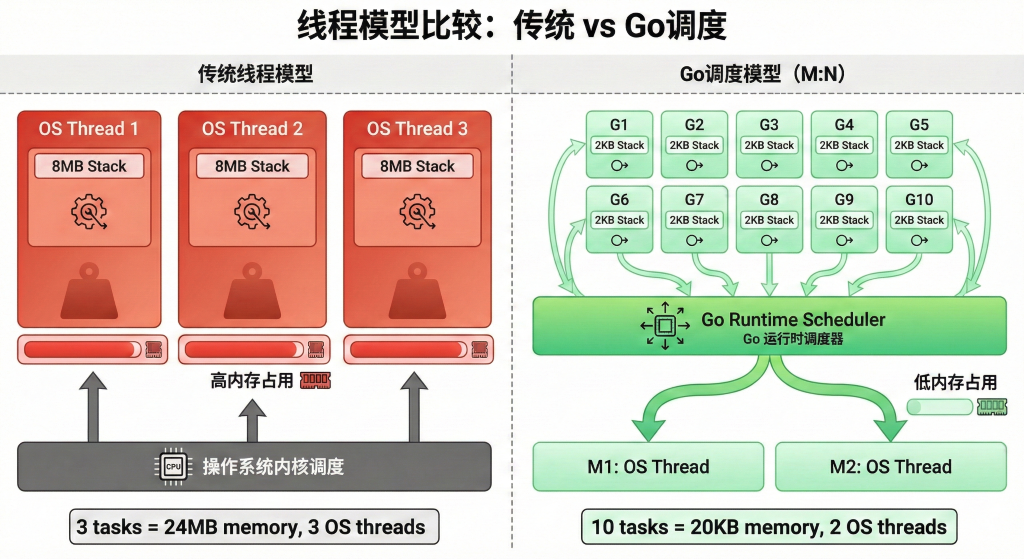
\includegraphics[width=1.0\linewidth]{figures/sec3/image3-2.png}
    \caption{传统操作系统线程模型与Go的M:N调度模型对比：Goroutine通过用户态调度实现高并发低开销}
    \label{fig:goroutine-model}
\end{figure}

Go语言通过Goroutine提供了一种更轻量的并发原语来解决传统线程模型的性能瓶颈。Goroutine是Go运行时在用户态管理的协程（coroutine），其核心设计理念是将并发执行单元的创建和调度从操作系统内核上移到语言运行时层面，从而获得更细粒度的控制能力和更低的资源开销。Goroutine的优势体现在多个维度。首先是极低的内存占用，每个Goroutine的初始栈空间仅2KB，相比操作系统线程的1到8MB栈空间，内存效率提升了数百倍。更重要的是，Goroutine的栈空间可以根据实际需要动态增长和收缩，避免了预分配大块内存导致的浪费。这使得在单机上同时运行数万甚至数十万个Goroutine成为可能，为"One Goroutine Per Connection"的架构模式提供了资源保障。

其次是高效的M:N调度模型。Go运行时维护少量操作系统线程（记为M），在其上调度大量Goroutine（记为N），形成M:N的多对多映射关系。这种设计的核心价值在于解耦了逻辑并发度和物理并行度。当某个Goroutine因等待I/O操作（如网络读取、数据库查询）而阻塞时，Go调度器会自动将其挂起并将该操作系统线程分配给其他可运行的Goroutine继续执行，而不是让整个线程进入阻塞状态。这种协作式调度机制使得I/O等待不再导致线程资源的浪费，CPU可以持续处理就绪的任务，显著提升了资源利用率。对于I/O密集型的游戏服务器，这意味着即使有数千个Goroutine在等待网络响应或数据库查询，实际占用的操作系统线程数仍然可以维持在几十个到几百个的合理范围内，避免了线程爆炸问题。

最后是简化的编程模型。开发者只需用\texttt{go}关键字启动并发任务，无需手动管理线程的创建、销毁、同步等底层细节，Go运行时负责所有调度策略和资源管理。这种抽象大幅降低了并发编程的心智负担，使得并发逻辑的表达更加接近业务语义。在游戏服务器的场景下，可以直接用"为每个玩家连接启动一个Goroutine"的自然表达来组织代码，而不需要考虑线程池大小、任务队列长度等底层实现细节。

为了直观展示Goroutine带来的性能提升，我们通过对比实验来量化顺序执行与并发执行的差异。假设需要为3名玩家分别执行一个耗时2秒的数据加载操作（如从数据库读取装备信息并进行复杂计算）。在顺序执行版本中，服务器必须等待玩家A的操作完全完成后，才能开始处理玩家B的请求，玩家C则需要等待前两个请求全部完成。这种串行处理模式导致总执行时间是单次操作时间的线性累加，三名玩家的总耗时达到6秒。对于实时游戏，6秒的等待意味着玩家C会看到明显的卡顿，严重影响用户体验。

% \begin{tcolorbox}[title=顺序执行模式的性能瓶颈]
% \begin{verbatim}
% func handlePlayer(playerID string) {
%     fmt.Printf("开始处理玩家 %s...\n", playerID)
%     time.Sleep(2 * time.Second) // 模拟I/O等待
%     fmt.Printf("玩家 %s 处理完成\n", playerID)
% }

% func main() {
%     startTime := time.Now()
%     // 顺序处理3名玩家
%     handlePlayer("A")
%     handlePlayer("B")
%     handlePlayer("C")
%     fmt.Printf("总耗时: %v\n", time.Since(startTime))
% }
% // 输出：总耗时约6秒，玩家C需要等待4秒才开始被处理
% \end{verbatim}
% \end{tcolorbox}

\begin{tcolorbox}[title=顺序执行模式的性能瓶颈]
\begin{lstlisting}[style=codeblock, language=go]
func handlePlayer(playerID string) {
    fmt.Printf("处理玩家 %s\n", playerID)
    time.Sleep(2 * time.Second) // 模拟数据库查询等I/O操作
}

func main() {
    handlePlayer("A")
    handlePlayer("B")
    handlePlayer("C")
    // 总耗时约6秒：每个玩家必须等待前一个处理完毕
}
\end{lstlisting}
\end{tcolorbox}

而通过\texttt{go}关键字启动Goroutine，三个处理任务可以并发执行，总耗时降低到单次操作的时间。在这个模式下，三个Goroutine由Go调度器分配到可用的操作系统线程上并发执行。如果服务器配备多核处理器，这些Goroutine可以实现真正的并行计算。即使在单核处理器上，由于操作主要是I/O等待而非CPU计算，调度器也可以在等待期间切换到其他Goroutine，充分利用等待时间。更重要的是，这种模式可以无缝扩展到50人、100人，只要单机CPU和内存资源充足，就能维持相近的响应延迟。

\begin{tcolorbox}[title=Goroutine并发模式的性能提升]
\begin{lstlisting}[style=codeblock, language=go]
func main() {
    var wg sync.WaitGroup
    players := []string{"A", "B", "C"}
    
    for _, player := range players {
        wg.Add(1)
        go func(id string) {
            defer wg.Done()
            handlePlayer(id)
        }(player)
    }
    
    wg.Wait()
    // 总耗时约2秒：三个玩家并发处理
}
\end{lstlisting}
\end{tcolorbox}

表\ref{tab:goroutine-performance}展示了顺序执行与并发执行在不同玩家规模下的性能对比。可以看到，当玩家数从3人增长到1000人时，顺序执行的总耗时呈线性增长，而并发执行的耗时基本保持稳定。这种差异在大规模场景下尤为显著，性能提升可达数百倍。

\begin{table}[h]
\centering
\caption{顺序执行与Goroutine并发的性能对比}
\label{tab:goroutine-performance}
\begin{tabular}{lccc}
\hline
\textbf{处理模式} & \textbf{3个玩家} & \textbf{1000个玩家} & \textbf{性能提升比} \\
\hline
顺序执行（串行） & 6秒 & 约2000秒（33分钟） & --- \\
Goroutine并发 & 2秒 & 2--3秒 & 约600--1000倍 \\
\hline
\end{tabular}
\end{table}

在实际的游戏服务器架构中，存在两种典型的Goroutine组织模式。One Goroutine Per Connection模式为每个WebSocket连接分配一个独立的Goroutine，负责该连接从建立到断开的完整生命周期，包括读取客户端消息、解析协议、执行业务逻辑、发送响应等操作。这种模式的优势在于连接的所有状态和上下文都封装在一个Goroutine内部，逻辑清晰且易于管理。One Goroutine Per Request模式则更进一步，即使在同一连接内，也可以为每个独立的业务请求（如发起战斗、查询背包、交易物品）启动临时Goroutine，任务完成后由Go运行时自动回收资源。这种模式适合请求处理时间差异较大的场景，可以避免慢请求阻塞连接上的其他快速请求。在实际工程中，这两种模式往往结合使用，连接层采用Per Connection模式维护长连接状态，业务层根据操作复杂度选择性地使用Per Request模式。

需要注意的是，Goroutine虽然轻量，但并非零成本。每个Goroutine仍然需要占用一定的内存空间和调度器资源，大量创建和销毁仍会给调度器和垃圾回收器带来压力。因此在后续章节中，我们会讨论对象池等优化手段来缓解这些开销。但总体而言，Goroutine提供的轻量级并发能力，为构建高并发游戏服务器奠定了坚实的资源基础，使得"每连接一协程"的架构模式在资源消耗和开发效率之间取得了理想的平衡。

% \subsubsection{Channel：消息沟通取代共享内存}

% \subsubsection{Channel：Goroutine 之间的通信机制}

\subsubsection{Channel：事件驱动的协程通信机制}

引入Goroutine解决了"如何高效并发"的问题，但随之而来的是新的挑战：并发的Goroutine之间如何安全地交换数据和协调执行顺序？传统多线程编程中，通常通过共享内存加锁的方式实现通信——多个线程直接访问同一块内存区域，通过互斥锁保护临界区来避免数据竞争。这种模式虽然直观，但容易引发死锁、优先级反转、数据竞争等难以调试的并发Bug，尤其在复杂的业务逻辑中，锁的获取顺序稍有不慎就可能导致系统陷入僵局。

Go语言倡导的并发哲学是："不要通过共享内存来通信，而应该通过通信来共享内存"。这一理念强调将数据的所有权在Goroutine之间显式传递，而非让多个Goroutine同时持有对同一数据的引用。这种设计哲学的载体就是Channel——Go提供的一种类型安全的消息队列，专门用于Goroutine之间传递数据。Channel的本质是一个先进先出的队列，配合发送和接收操作的阻塞语义，可以自然地实现Goroutine之间的同步和协调。

Channel分为无缓冲通道和有缓冲通道两种类型，两者在同步语义上有本质区别。无缓冲通道要求发送和接收操作必须同时就绪才能完成，具有强同步语义。当一个Goroutine向无缓冲通道发送数据时，它会阻塞等待直到另一个Goroutine从该通道接收数据，这种"握手"机制可以精确控制Goroutine之间的执行顺序。有缓冲通道则允许在缓冲区未满时异步发送数据，缓冲区未空时异步接收数据。发送方只有在缓冲区满时才会阻塞，接收方只有在缓冲区空时才会阻塞。有缓冲通道的价值在于解耦生产者和消费者的处理速度，允许短时间内的速率差异，避免生产者因消费者处理较慢而被频繁阻塞。

在游戏服务器开发中，Channel的典型应用场景是将玩家操作事件异步分发给处理协程，实现网络I/O层和业务逻辑层的解耦。考虑这样的架构设计：每个玩家连接对应一个读取Goroutine（负责从WebSocket读取消息并反序列化）和一个处理Goroutine（负责执行业务逻辑如移动验证、战斗计算、状态更新）。两者通过一个有缓冲的Channel连接，读取Goroutine将解析后的消息对象发送到Channel，处理Goroutine从Channel接收消息并执行相应逻辑。

\begin{tcolorbox}[title=使用Channel实现消息异步处理]
\begin{lstlisting}[style=codeblock, language=go]
type PlayerMessage struct {
    PlayerID string
    Action   string
    Data     interface{}
}

func handlePlayerConnection(playerID string) {
    msgChan := make(chan PlayerMessage, 100)
    
    go func() {
        for msg := range msgChan {
            processMessage(msg)
        }
    }()
    
    // 接收并发送消息到channel
    for i := 0; i < 5; i++ {
        msgChan <- PlayerMessage{
            PlayerID: playerID,
            Action:   "move",
            Data:     fmt.Sprintf("position:%d", i),
        }
    }
    
    close(msgChan)
}
\end{lstlisting}
\end{tcolorbox}

这种设计带来了多个层面的架构优势。首先是读写解耦，网络I/O和业务逻辑完全分离为独立的执行流。读取Goroutine专注于高效地从网络套接字读取字节流并进行协议解析，不需要等待业务逻辑执行完成就可以继续接收下一条消息。即使业务处理较慢（如涉及复杂的战斗计算或数据库查询），也不会阻塞消息接收，保证了系统的响应性。其次是流量控制，有缓冲的Channel可以平滑瞬时流量峰值。当玩家在短时间内连续发送多条操作指令时（如快速点击技能按钮），这些消息会被暂存在Channel的缓冲区中，处理Goroutine可以按照自己的节奏从缓冲区取出消息依次处理，避免了生产者速率过快导致的消费者过载问题。最后是优雅关闭，通过\texttt{close(channel)}可以通知所有接收方停止等待。当连接断开时，读取Goroutine关闭消息Channel，处理Goroutine在处理完缓冲区中的剩余消息后会感知到通道已关闭，自动退出循环并进行资源清理。这种基于通道关闭的退出机制比通过共享标志位检查更加简洁和可靠。

\begin{figure}[H]
    \centering
    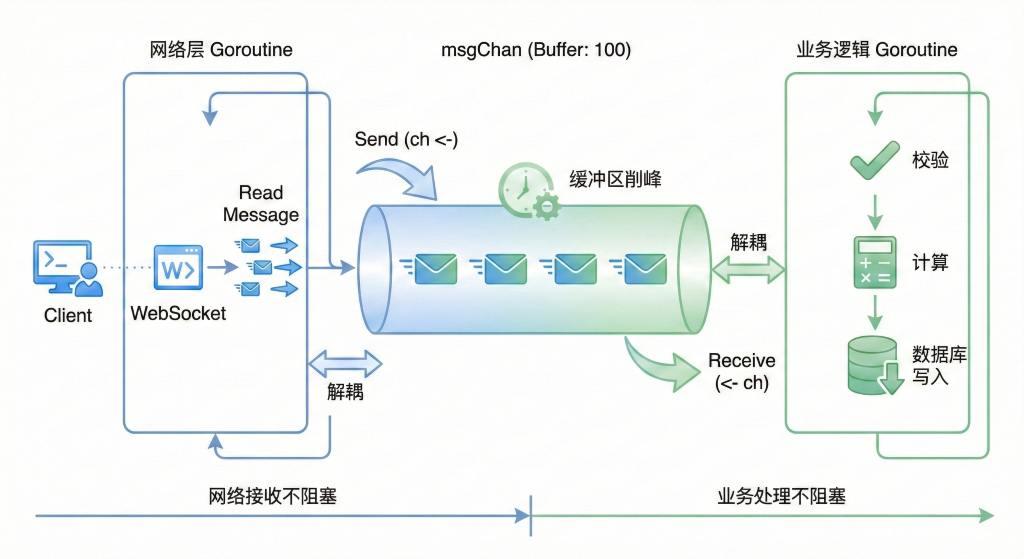
\includegraphics[width=1\linewidth]{figures/sec3/image3-3.png}
    \caption{基于Channel的消息异步处理架构：网络I/O与业务逻辑解耦，实现流量削峰和非阻塞处理}
    \label{fig:channel-async}
\end{figure}

当需要同时监听多个Channel或处理超时时，Go提供了\texttt{select}语句进行多路复用。\texttt{select}语句在语法上类似于\texttt{switch}，但每个\texttt{case}分支对应一个通道操作（发送或接收）。\texttt{select}会阻塞等待直到至少有一个\texttt{case}分支的通道操作可以执行，如果多个\texttt{case}同时就绪，则随机选择一个执行。这种机制在游戏服务器中可用于实现超时控制和心跳检测。

\begin{tcolorbox}[title=使用Select实现超时控制]
\begin{lstlisting}[style=codeblock, language=go]
func handleWithTimeout(playerID string, msgChan chan PlayerMessage) {
    for {
        select {
        case msg := <-msgChan:
            processMessage(msg)
        case <-time.After(30 * time.Second):
            fmt.Printf("玩家 %s 超时，断开连接\n", playerID)
            return
        }
    }
}
\end{lstlisting}
\end{tcolorbox}

在这个示例中，\texttt{select}语句同时监听两个事件源：消息Channel和超时定时器。如果30秒内\texttt{msgChan}收到新消息，则执行第一个\texttt{case}分支进行正常处理；如果30秒内没有任何消息到达，\texttt{time.After}会向其返回的通道发送一个时间值，触发第二个\texttt{case}分支执行超时处理逻辑。这种模式在游戏服务器中用于实现心跳检测：如果玩家长时间不发送任何消息（包括心跳包），服务器会主动断开连接释放资源，防止僵尸连接占用系统资源。

从系统设计的角度看，Channel提供的是一种事件驱动的并发架构模式，这种模式与Actor模型有异曲同工之处。每个Goroutine可以被视为一个独立的执行单元，它们不直接访问彼此的内存空间，而是通过发送消息来协作完成复杂任务。这种基于消息传递的并发模型天然地降低了数据竞争风险，因为数据的所有权在不同Goroutine之间显式转移，避免了多个执行流同时修改同一数据的情况。更重要的是，这种架构模式为后续的分布式扩展埋下了平滑演进的伏笔。当系统从单机演化为多机时，Goroutine之间的Channel可以被替换为跨网络的RPC调用或消息队列（如Kafka、RabbitMQ），而业务逻辑的组织方式基本保持不变。这种从进程内通信到进程间通信、从单机并发到分布式并发的平滑过渡，正是基于消息传递的并发模型的核心价值所在。

然而，引入Goroutine和Channel后，我们获得了并发处理多人请求的能力，但并发也带来了新的风险。当多个Goroutine需要访问同一份共享数据时，如何保证操作的原子性与结果的确定性？这正是下一节要解决的核心问题——并发环境下的规则可信度保障。


% \paragraph{写作建议}
% \begin{enumerate}
%     \item 要先讲 单线程 的痛点，引出并发作用（同时处理多请求），点出 goroutine（协程） 轻量优势。
%     \item 讲清goroutine和Channel的协作逻辑：
%     \paragraph{}在游戏场景中，单一 goroutine 处理所有玩家请求会导致性能瓶颈，因为玩家的操作请求（如移动、攻击等）是并发产生的。采用多 goroutine 模式，为每个玩家分配独立的 goroutine（如玩家 1 的请求由专属 goroutine 处理），能并行处理不同玩家的操作，大幅提升系统响应速度。
%     \paragraph{} 当多个 goroutine 同时访问和修改共享数据（例如双玩家争抢地图上同一位置资源）时，会出现数据竞争问题，导致游戏状态混乱。通过 Channel 传递数据，可将并发访问限制为顺序执行：数据的生产和消费通过 Channel 进行同步，只有当接收方准备好时，发送方才能传递数据，从而避免多个 goroutine 同时修改同一数据，有效解决数据竞争带来的冲突问题，确保游戏状态的一致性和稳定性。
%     \item 铺垫锁：操作同一资源需加锁，为 3.3 做准备。
% \end{enumerate}

\subsection{混乱中的秩序：“锁"住你的虚拟宝藏}

在上一节中，我们通过Goroutine实现了"每个玩家独立处理"的并发模型，显著提升了系统吞吐量。但并发带来新能力的同时，也引入了新的风险：当多个Goroutine需要访问同一份共享数据时，如何保证操作的原子性与结果的确定性？这不仅仅是编程技巧问题，更是多人在线游戏规则可信度的工程基础。在游戏这种强对抗性的环境中，任何规则的不确定性都会被玩家直接感知并放大为体验问题，甚至引发对系统公平性的质疑。

\subsubsection{当两个玩家同时捡起一把剑}

考虑这样一个典型场景：地图上刷新了一把稀有武器（如传说级屠龙刀），系统中仅存在这唯一的一把。同一时刻，玩家A和玩家B几乎同时触发了拾取操作。从玩家的业务视角看，这是一个简单的"先到先得"规则——谁先完成拾取动作，谁就应该获得该装备，另一名玩家则应该看到"物品已被拾取"的提示。但从系统实现的角度看，这个看似简单的业务规则背后涉及一系列并发操作的正确协调。玩家A的Goroutine首先读取全局的\texttt{hasItem}标志，发现其值为\texttt{true}，判定物品存在，随即开始执行拾取逻辑。几乎在同一时刻，玩家B的Goroutine也读取\texttt{hasItem}标志，同样发现其值为\texttt{true}，也通过了存在性检查并进入拾取流程。随后，两个Goroutine分别将\texttt{hasItem}设为\texttt{false}，并各自在内存中更新了所属玩家的背包数据。从执行结果看，两个玩家的客户端都收到了"拾取成功"的响应，但实际上地图上只有一把武器，这违反了物品唯一性的核心规则。

这种现象在并发编程中被称为竞态条件（Race Condition），其根源在于"检查-修改"这一组合操作不是原子的。在玩家A检查到物品存在与将标志设为\texttt{false}之间，存在一个时间窗口。如果玩家B的检查操作落在这个窗口内，两个Goroutine都会通过检查条件并执行修改操作，导致同一资源被多次获取。这种并发访问冲突不仅破坏了游戏内物品的唯一性约束，还可能引发更严重的连锁问题。如果这把稀有武器是限量发行的活动奖励，复制物品会破坏游戏的经济系统平衡，影响其他正常玩家的游戏体验。如果涉及交易系统，一个物品被多个玩家持有可能导致交易记录混乱，甚至引发玩家之间的纠纷。

竞态条件问题并非游戏服务器特有，而是所有需要保证业务规则只产生唯一结果的并发系统都必须面对的核心挑战。在电商系统中，库存扣减操作必须保证原子性，否则会出现超卖现象——实际库存只有10件商品，但由于并发扣减时多个订单同时通过了库存检查，最终可能生成15个订单。在金融系统中，账户转账操作涉及扣减发送方余额和增加接收方余额两个步骤，如果这两个操作不能原子执行，系统在崩溃或并发冲突时可能出现资金凭空消失或凭空增加的双花问题。在协同编辑系统中，多个用户同时修改文档的同一段落，如果缺乏冲突检测和合并机制，可能出现后提交的修改覆盖先提交修改的数据丢失问题。

对于游戏服务器而言，竞态条件的后果尤为严重，因为它直接体现为玩家可感知的规则失效。两人同时拾取导致物品复制，玩家会质疑游戏的公平性；同时攻击导致伤害计算重复，受害玩家会认为遭遇了Bug或外挂；同时占领据点导致归属混乱，团队战术配合会因系统不可预测性而失去意义。这些问题的本质是：在并发环境下，我们需要一种机制来保证关键的业务规则修改是串行执行的，即使多个Goroutine试图同时操作，也只能有一个成功，其他必须等待或收到明确的失败反馈。这正是互斥锁要解决的核心问题。

\subsubsection{实战：没有锁的混乱现场}

让我们通过代码重现这个问题，更直观地理解竞态条件的危害。在下面的示例中，全局变量\texttt{hasItem}表示地图上是否存在可拾取的物品。\texttt{pickItem}函数模拟玩家拾取逻辑，包括检查物品是否存在、模拟处理延迟（如网络往返或数据库写入）、标记物品已被拾取三个步骤。

\begin{tcolorbox}[title=危险代码：缺乏同步保护的并发访问]
\begin{lstlisting}[style=codeblock, language=go]
var hasItem = true // 全局标志：地图上是否有物品

func pickItem(playerID string) {
    if hasItem { // 步骤1：检查物品是否存在
        time.Sleep(time.Millisecond) // 步骤2：模拟延迟
        hasItem = false // 步骤3：标记已拾取
        fmt.Printf("玩家 %s 成功拾取物品\n", playerID)
    } else {
        fmt.Printf("玩家 %s 拾取失败，物品已被抢走\n", playerID)
    }
}

func main() {
    go pickItem("A") // 玩家A的Goroutine
    go pickItem("B") // 玩家B的Goroutine
    time.Sleep(time.Second) // 等待两个Goroutine执行完毕
}
\end{lstlisting}
\end{tcolorbox}

运行这段代码多次，大概率会看到两名玩家都"成功"拾取了物品，少数情况下才会出现正确的结果（一成功一失败）。问题的关键在于步骤1的检查和步骤3的修改之间存在明显的时间窗口。当玩家A执行到步骤1发现\texttt{hasItem=true}后，在执行步骤2的延迟期间，玩家B也执行了步骤1同样发现为\texttt{true}。结果两者都通过了检查条件，进入拾取分支。即使步骤2的延迟很短（只有1毫秒），在高并发场景下这个窗口仍然足够让多个Goroutine同时通过检查。这种并发访问冲突导致同一件稀有装备被多次获取，破坏了游戏内物品的唯一性约束。从更深层次看，这个问题暴露了一个根本性矛盾：在并发环境下，我们需要的不仅是"每个Goroutine都能独立执行"，更需要"对于某些关键操作，多个Goroutine必须排队等待"。如何在保持并发处理能力的同时，对特定的共享资源访问进行串行化控制，这正是下一小节要解决的问题。

\subsubsection{互斥锁：将规则修改收敛为原子操作}

要解决上述竞态条件问题，核心思路是将"检查-修改"这一组合操作变成不可分割的原子区，保证在同一时刻只有一个Goroutine能够执行这段逻辑。互斥锁（Mutex, Mutual Exclusion Lock）正是实现这一目标的基本同步原语。互斥锁的工作机制类似于一个只能同时被一个人持有的令牌：当一个Goroutine需要访问共享资源时，它首先尝试获取锁（调用\texttt{Lock()}方法）；如果锁当前没有被其他Goroutine持有，则成功获取并进入临界区执行关键操作；如果锁已被其他Goroutine持有，则当前Goroutine进入阻塞等待状态，直到持有锁的Goroutine完成操作并释放锁（调用\texttt{Unlock()}方法）。

在Go中，标准库提供了\texttt{sync.Mutex}类型来实现互斥锁。其设计非常简洁，只提供两个核心方法：\texttt{Lock()}用于获取锁，如果锁不可用则阻塞；\texttt{Unlock()}用于释放锁，允许其他等待的Goroutine获取。需要注意的是，对同一个Mutex多次调用\texttt{Lock()}而不释放会导致死锁，因此推荐使用\texttt{defer}语句确保锁一定会被释放，即使函数因\texttt{return}或\texttt{panic}提前退出也不会遗漏。

\begin{figure}[H]
    \centering
    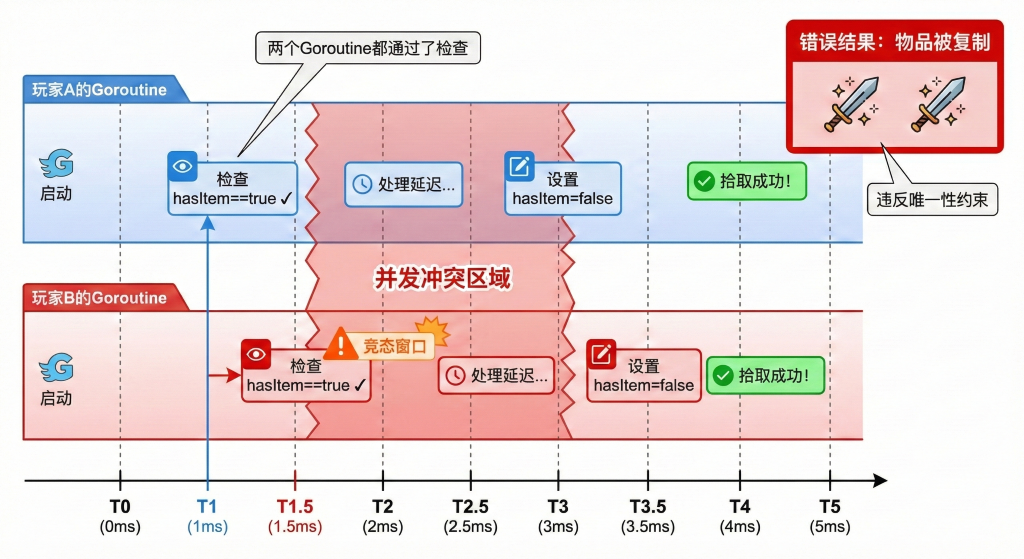
\includegraphics[width=1\linewidth]{figures/sec3/image3-4.png}
    \caption{竞态条件的时序分析：缺乏同步保护导致两个Goroutine同时通过检查并修改共享状态}
    \label{fig:race-condition}
\end{figure}

\subsubsection{实战：加上锁的秩序世界}

现在我们引入\texttt{sync.Mutex}来修复前面的竞态条件问题。在\texttt{pickItemSafe}函数中，通过\texttt{itemLock.Lock()}加锁进入临界区，使用\texttt{defer itemLock.Unlock()}确保无论函数如何退出锁都会被释放。这样，整个"检查-修改"过程被保护在一个原子操作内。

\begin{tcolorbox}[title=安全代码：使用Mutex保护共享资源]
\begin{lstlisting}[style=codeblock, language=go]
var hasItem = true
var itemLock sync.Mutex // 互斥锁

func pickItemSafe(playerID string) {
    itemLock.Lock() // 获取锁，进入临界区
    defer itemLock.Unlock() // 延迟释放锁
    
    if hasItem {
        time.Sleep(time.Millisecond) // 模拟处理延迟
        hasItem = false
        fmt.Printf("玩家 %s 成功拾取物品\n", playerID)
    } else {
        fmt.Printf("玩家 %s 拾取失败，物品已被抢走\n", playerID)
    }
}

func main() {
    go pickItemSafe("A")
    go pickItemSafe("B")
    time.Sleep(time.Second)
}
\end{lstlisting}
\end{tcolorbox}

现在运行结果变为确定性的：玩家A成功拾取物品，玩家B拾取失败。规则恢复了可信度。通过引入互斥锁机制，原本可能并发执行的多个拾取操作被串行化为顺序执行。当玩家A的Goroutine获取锁后，玩家B的Goroutine在尝试获取锁时会被阻塞，直到玩家A完成整个操作并释放锁。这样，无论两个Goroutine的启动时间多么接近，它们对共享资源的访问都会被强制排队，从而保证了在任意时刻只有一个协程能够访问和修改共享数据。\texttt{defer itemLock.Unlock()}的设计是一个重要的工程实践，它利用了Go语言的defer机制，确保即使函数在执行过程中发生\texttt{panic}或通过\texttt{return}提前返回，锁也一定会被释放，避免了其他Goroutine永久阻塞导致的死锁问题。

在使用互斥锁时需要注意几个重要的实现细节和潜在陷阱。首先，Mutex必须通过指针方式传递给函数或作为结构体字段使用。如果按值传递Mutex，会导致锁被复制，每个Goroutine实际上操作的是不同的锁副本，同步保护完全失效。其次，临界区的范围应该尽可能小，只保护必须同步的共享数据访问，而将不需要同步的计算逻辑移出临界区。过大的临界区会导致Goroutine长时间持有锁，降低并发度，使系统性能退化接近单线程。最后，要避免嵌套锁的使用，即在持有锁A的情况下又尝试获取锁B，这很容易因为不同Goroutine的加锁顺序不一致而导致死锁。如果业务逻辑确实需要同时访问多个资源，应该定义明确的加锁顺序并严格遵守。

\subsubsection{锁的粒度：性能与公平的折中设计}

虽然互斥锁解决了并发环境下的正确性问题，但也引入了新的性能成本：串行化。被锁保护的代码块在同一时刻只能被一个Goroutine执行，其他Goroutine必须排队等待。这种串行化执行意味着并发度的降低，如果临界区执行时间较长或访问频率很高，锁竞争会成为系统瓶颈。因此，在实际系统设计中，锁的粒度选择成为一个需要仔细权衡的问题，它本质上是在并发性能和实现复杂度之间寻找平衡点。

\begin{figure}[H]
    \centering
    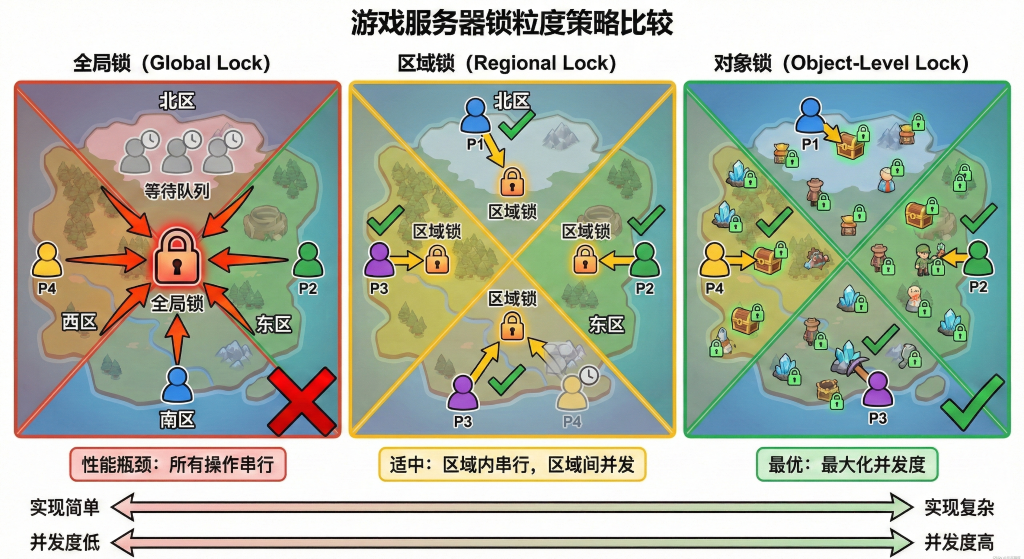
\includegraphics[width=1\linewidth]{figures/sec3/image3-5.png}
    \caption{锁粒度的三种策略对比：全局锁实现简单但性能差，对象锁并发度高但复杂度增加}
    \label{fig:lock-granularity}
\end{figure}

全局锁是最简单粗暴的方案，整个服务器共用一把大锁，所有涉及共享状态的操作都必须获取这把锁才能执行。这种方式的优势是实现极其简单，几乎不可能出现死锁或其他复杂的并发Bug，因为所有并发操作本质上被强制转换为了单线程顺序执行。然而，其代价是所有玩家的操作都要排队等待，即使这些操作实际上访问的是完全独立的资源（如玩家A在地图北边拾取物品，玩家B在地图南边打怪），也必须依次执行。这导致系统性能完全退化回单线程模型，失去了引入并发的全部意义。因此，全局锁仅适用于访问频率极低的全局配置读取、服务器启动关闭等特殊场景，在核心游戏逻辑中应该坚决避免。

细粒度锁则走向了另一个极端，为每个独立的资源实例分配独立的锁。在游戏服务器中，这意味着每个玩家的状态（血量、背包、位置）由各自的Mutex保护，每个地图上的可交互对象（宝箱、NPC、资源节点）也持有独立的锁。这样一来，玩家A拾取屠龙刀时只锁定该物品，完全不影响玩家C在旁边打怪的操作；玩家B在商城购物时使用的是自己背包的锁，不影响玩家D在竞技场对战时访问角色属性。细粒度锁能够最大化系统的并发度，允许大量操作真正并行执行，是高并发游戏服务器的理想选择。然而，其实现复杂度也显著增加，主要体现在两个方面。一是锁的数量激增，管理和维护成本上升，容易遗漏某些应该保护的共享数据。二是当一个操作需要同时访问多个资源时（如玩家A攻击玩家B，需要同时锁定双方的状态），必须非常小心地设计加锁顺序，否则容易产生死锁。

区域锁在全局锁和细粒度锁之间取得折中，是实践中较为常见的选择。典型的做法是将游戏世界划分为多个逻辑区域（如地图分块、副本实例），每个区域由独立的Mutex保护。区域内的操作需要串行执行，但不同区域之间的操作可以并发进行。这种粒度既避免了全局锁的性能瓶颈，又比细粒度锁更易于管理，在并发度和实现复杂度之间达到了合理的平衡。在具体实施时，区域的划分需要根据游戏的空间局部性特征来设计，尽量保证大多数玩家交互发生在同一区域内，跨区域操作相对较少。

表\ref{tab:lock-granularity}总结了不同锁粒度在游戏服务器中的典型应用场景与性能特点。在实际工程中，往往会混合使用多种粒度的锁，根据不同资源的访问特征选择合适的保护策略。

\begin{table}[h]
\centering
\caption{不同锁粒度的应用场景与性能对比}
\label{tab:lock-granularity}
\begin{tabular}{p{3cm}p{5cm}p{4cm}}
\hline
\textbf{锁的粒度} & \textbf{应用场景} & \textbf{并发性能} \\
\hline
全局锁 & 服务器配置读取、全服公告 & 严重阻塞，接近单线程 \\
区域锁 & 地图分块、副本实例 & 中等，区域间可并发 \\
对象锁 & 单个玩家数据、单个物品 & 最优，最大化并发度 \\
\hline
\end{tabular}
\end{table}

需要特别强调的是，本节讨论的\texttt{sync.Mutex}只能保护单个进程内的数据，其同步机制依赖于进程内的共享内存，无法跨越网络边界。当系统进入第四章的分布式阶段，多台服务器需要协同工作时，跨服务器的状态同步需要引入分布式锁（如基于Redis的\texttt{SETNX}命令实现的分布式互斥）或更复杂的分布式一致性协议（如Raft、Paxos）。但在当前的单机阶段，\texttt{sync.Mutex}已经足够让我们建立起并发环境下的规则可信度保障，为游戏世界筑起第一道并发安全的防线。通过合理设计锁的粒度和临界区范围，可以在正确性和性能之间取得理想的平衡，为后续的性能优化奠定坚实基础。



% \subsection{混乱中的秩序：“锁” 住你的虚拟宝藏}
% \paragraph{本节目标} 理解数据竞争危害，掌握 “单机锁 + 分布式锁” 逻辑，明确不同场景下锁的粒度选择。
% \paragraph{写作建议} 
% \begin{enumerate}
%     \item 以 “双玩家抢道具都拿到” 痛点，引出锁作用（同一时间 1 个操作改数据）。
%     \item 介绍分两类锁：
%     \paragraph{单机锁} 适用于同服务器内多 goroutine 竞争场景，例如游戏内角色背包物品增减、任务进度更新等高频操作。采用细粒度锁，针对单个玩家数据或具体功能模块加锁（如背包锁、任务锁），避免因全局锁导致性能瓶颈。
%     \paragraph{分布式锁} 随着游戏规模扩大，当第四章提及的多服务器协作需求出现，如跨服竞技排名更新、全服活动资源分配等场景，单机锁已无法满足需求。此时使用 Redis 实现分布式锁，可解决多服务器间竞争问题。建议采用粗粒度锁，对涉及全局数据变更的操作整体加锁，减少锁冲突开销，但需注意控制锁的范围，防止影响并发性能。
% \end{enumerate}


\subsection{敞开大门：让服务器迎接成千上万的玩家}

在前两节中，我们系统性地解决了单机服务器在多人同图场景下的两大核心问题。通过Goroutine和Channel，我们建立了并发处理大量玩家请求的表达能力，使服务器不再受限于顺序执行的吞吐瓶颈。通过Mutex等同步原语，我们保证了并发环境下游戏规则的正确性，确保共享资源的访问产生唯一、确定的结果。然而，当这两个问题解决后，单机服务器的瓶颈会从"算不过来"转向新的三个方向：第一是"连不过来"，频繁建立和销毁连接消耗大量系统资源，当每秒需要处理数千次连接操作时，TCP握手和挥手的开销会成为显著的性能拖累；第二是"扛不住"，大量临时对象的创建给垃圾回收器带来压力，频繁的GC暂停会导致响应延迟出现不可预测的抖动；第三是"抖得厉害"，数据访问路径的延迟不稳定影响玩家体验，所有数据都访问磁盘数据库会因I/O瓶颈导致响应时间恶化。本节将从连接层、内存层、数据层三个维度，系统性地提升单机服务器的承载上限，完成从"能并发"到"能承载"的关键跨越。

\subsubsection{连接管理：从短连接到连接池的资源复用}

每次建立TCP连接都需要完成三次握手过程，这涉及客户端和服务器之间的三次网络往返：客户端发送SYN包，服务器回复SYN-ACK包，客户端再发送ACK包确认。每个握手步骤都涉及系统调用，需要在用户态和内核态之间切换，还需要分配内核资源如套接字缓冲区、连接控制块等数据结构。按照典型的网络延迟估算，局域网环境下每次握手往返约需1毫秒，广域网环境可能达到几十毫秒。如果在每次数据交互时都重新建立连接，然后在交互完成后立即关闭，这种短连接模式会导致严重的性能问题和资源浪费。

在高并发场景下，缺乏连接复用机制会带来多方面的负面影响。当服务器每秒需要处理10,000次数据库查询时，如果每次查询都建立新连接，就需要执行10,000次TCP三次握手和10,000次四次挥手操作。按照平均每次握手耗时1到3毫秒计算，仅握手过程就会累计消耗10到30秒的CPU时间，这些时间本可以用于实际的业务逻辑处理。更严重的问题在于端口资源的耗尽。操作系统为每个TCP连接分配一个临时端口号，端口号的范围通常在1024到65535之间，可用端口约为6万个。当连接关闭后，该端口会进入\texttt{TIME\_WAIT}状态，持续约1到2分钟以确保网络中延迟到达的数据包不会干扰新连接。如果每秒创建和销毁数千个连接，这些处于\texttt{TIME\_WAIT}状态的连接会迅速占满可用端口池，导致新连接无法建立，服务器实质性不可用。此外，频繁的连接创建还会给操作系统的连接跟踪表（如Linux的conntrack）带来压力，在高并发场景下可能触发内核的资源限制，引发连接建立失败或超时。

连接池（Connection Pool）机制正是为了解决这一问题而设计的资源复用方案。连接池的核心思想是预先创建一定数量的长连接并维护在内存中，当业务逻辑需要访问外部资源（如数据库、缓存服务）时，不是临时创建新连接，而是从池中借出一个空闲连接使用。使用完成后，连接不会被销毁，而是归还到池中等待下次复用。只有当池中所有连接都在使用且达到配置的最大连接数上限时，新请求才需要等待或创建临时连接。Go语言标准库\texttt{database/sql}\footnote{\texttt{database/sql}是Go标准库提供的数据库访问接口包，定义了统一的数据库操作API并内置连接池管理功能。它采用驱动模式设计，通过导入特定数据库驱动（如\texttt{lib/pq}用于PostgreSQL，\texttt{go-sql-driver/mysql}用于MySQL）即可操作不同数据库，而无需修改业务代码。连接池的创建、维护、过期清理等复杂逻辑完全由该包自动处理，开发者只需通过\texttt{SetMaxOpenConns}、\texttt{SetMaxIdleConns}等方法配置参数即可。}内置了连接池管理功能，可以自动维护数据库连接的生命周期。


\begin{tcolorbox}[title=数据库连接池配置]
\begin{lstlisting}[style=codeblock, language=go]
func initDB() *sql.DB {
    db, _ := sql.Open("postgres", dsn)
    
    db.SetMaxOpenConns(100)        // 最大打开连接数
    db.SetMaxIdleConns(10)         // 最大空闲连接数
    db.SetConnMaxLifetime(time.Hour) // 连接最大生命周期
    
    return db
}
\end{lstlisting}
\end{tcolorbox}

这三个参数共同决定了连接池的行为特征。\texttt{MaxOpenConns}限制了同时打开的最大连接数，防止数据库服务器因连接过多而过载。当并发请求数超过这个限制时，多余的请求会进入等待队列。\texttt{MaxIdleConns}控制空闲连接的保留数量，这些连接在没有请求时仍然保持打开状态，可以立即响应新请求而无需重新握手。\texttt{ConnMaxLifetime}为连接设置最大存活时间，超过这个时间的连接会被自动关闭并替换为新连接，这可以避免长期运行的连接累积状态异常或资源泄漏。通过这样的配置，即使有10,000次查询请求，实际的TCP连接创建次数也被限制在100以内，大幅降低了握手开销和端口消耗。

\begin{figure}[H]
    \centering
    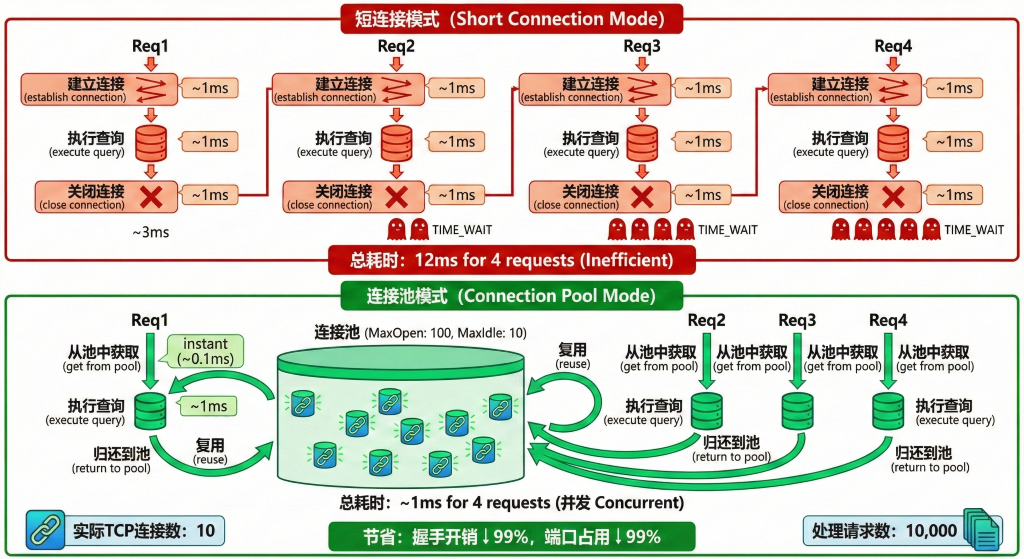
\includegraphics[width=1.0\linewidth]{figures/sec3/image3-6.png}
    \caption{连接池的资源复用机制：通过预创建和重用连接，消除频繁握手和挥手的开销}
    \label{fig:connection-pool}
\end{figure}

连接池的运作机制体现了资源池化管理的核心原则。当业务逻辑发起数据库查询时，连接池首先检查是否有空闲连接可用。如果存在空闲连接，则立即将其标记为占用状态并返回给调用方，整个过程只涉及内存操作，延迟在微秒级别。如果当前没有空闲连接但总连接数未达到上限，连接池会创建新连接并将其加入池中。如果已达到连接数上限，新请求会进入等待队列，直到有其他请求归还连接。当业务逻辑完成数据库操作后，调用连接的关闭方法，但这个"关闭"操作被连接池拦截，实际上只是将连接的状态标记为空闲，重新放入可用队列，而不是真正关闭TCP连接。通过这种"借出-归还"的循环，连接可以被成千上万次地复用，避免了反复握手和挥手的巨大开销。

从云计算的视角看，连接池体现的正是资源池化（Resource Pooling）的核心思想。这是云计算五大特征之一，强调将计算、存储、网络等资源抽象为可动态分配的共享池，按需分配，用完归还，从而最大化资源利用率并降低供给成本。连接池在微观层面实现了这一理念：将稀缺的连接资源组织为共享池，通过精细的生命周期管理实现高效复用。这种池化思想在云原生系统中随处可见，从虚拟机的资源池、容器的镜像缓存池，到负载均衡器的后端服务器池，都是同一设计模式在不同抽象层次的体现。

\subsubsection{对象池：用sync.Pool缓解GC压力}

除了外部连接资源，程序内部的临时对象分配也可能成为性能瓶颈。在游戏服务器的网络层实现中，需要频繁创建和销毁大量临时对象：每次接收网络消息需要分配字节缓冲区（\texttt{[]byte}）用于存储数据，每次解析协议需要创建请求上下文对象，每次序列化响应需要构造JSON编码器，每次日志记录需要分配格式化字符串。这些临时对象的生命周期通常只有几毫秒到几百毫秒，使用完成后立即成为垃圾。在高并发场景下，这些对象的分配和回收频率可能达到每秒数万次甚至数十万次，对Go运行时的垃圾回收器（GC）造成显著压力。

Go的垃圾回收器采用并发标记-清除算法，其设计目标是减少STW（Stop-The-World）暂停时间以保证程序的响应性。但GC并非零成本，每次GC周期仍然需要执行两次短暂的STW暂停：一次在标记开始阶段启用写屏障，一次在标记结束阶段完成最终标记。虽然单次STW时间通常在亚毫秒到几毫秒级别，但在内存分配速率很高的情况下，GC会更频繁地触发，累积的暂停时间会对延迟敏感的应用造成明显影响。对于实时游戏服务器，即使几十毫秒的延迟抖动也可能被玩家感知为卡顿，影响操作的流畅性和战斗判定的准确性。此外，GC在标记阶段需要遍历大量对象的引用关系，这会占用CPU资源并污染处理器缓存，间接降低业务逻辑的执行效率。

\texttt{sync.Pool}提供了一种轻量级的对象复用机制来缓解上述问题。\texttt{sync.Pool}是Go标准库提供的协程安全的对象池实现，专门用于缓存和复用临时对象。其工作原理是维护一个对象缓存，当业务代码需要临时对象时，优先从缓存中获取已有对象；使用完成后，将对象归还到缓存而非立即丢弃。通过这种复用机制，可以显著减少内存分配次数，从而降低GC的触发频率和工作负载。

\begin{tcolorbox}[title=使用sync.Pool复用临时对象]
\begin{lstlisting}[style=codeblock, language=go]
var bufferPool = sync.Pool{
    New: func() interface{} {
        return new(bytes.Buffer)
    },
}

func handleMessage(data []byte) {
    buf := bufferPool.Get().(*bytes.Buffer)
    buf.Reset()
    
    buf.Write(data)
    processData(buf.Bytes())
    
    bufferPool.Put(buf)
}
\end{lstlisting}
\end{tcolorbox}

\texttt{sync.Pool}的使用模式遵循"获取-使用-归还"的三段式流程。\texttt{Get()}方法尝试从池中取出一个对象，如果池中有缓存的对象则直接返回，如果池为空则调用\texttt{New}函数创建新对象。在使用对象之前，务必调用\texttt{Reset()}或类似方法清理对象的状态，确保不会受到之前使用者留下的脏数据影响。业务逻辑使用对象完成工作后，调用\texttt{Put()}方法将对象归还到池中。需要特别注意的是，\texttt{sync.Pool}中的对象不保证一定存在。Go运行时在GC时会清空\texttt{sync.Pool}中的所有对象，这是为了避免池中的对象阻碍GC回收其他内存。因此，\texttt{New}函数是必需的兜底机制，不能假设池中永远有对象可用。

\texttt{sync.Pool}的价值在于打破了"分配-使用-回收"的线性生命周期，将其改造为"分配-使用-缓存-复用"的循环模式。对于那些频繁创建且生命周期很短的对象，复用可以将分配频率从每次请求都分配降低到只在池为空时分配，大幅减少了需要被GC扫描和回收的对象数量。在实践中，合理使用\texttt{sync.Pool}可以将GC暂停时间降低50\%以上，对于追求低延迟的在线服务，这种优化带来的稳定性提升是显著的。然而，\texttt{sync.Pool}并非万能药，它只适合缓存"用完即可丢弃"的短命对象，不适合作为长期持有的状态存储。对于需要跨请求保留状态的数据，应该使用普通的数据结构或专门的缓存系统。

\subsubsection{缓存分层架构：热数据与冷数据的协同治理}

在连接层和内存层完成资源复用优化后，数据访问路径成为影响单机性能的最后一道关口。游戏服务器中的数据访问模式存在显著的频率差异：玩家的实时位置每秒可能更新数十次，在线状态每秒被查询数千次，这些高频数据要求毫秒级甚至亚毫秒级的响应延迟；而账号信息、历史成就、装备配置等数据可能几分钟甚至几小时才被访问一次，但对持久性和一致性有更高要求。如果所有数据都存储在磁盘数据库中，每次查询都需要等待磁盘I/O，在高并发场景下会迅速达到数据库的IOPS上限，导致查询排队和响应延迟恶化。反之，如果所有数据都存储在内存中，虽然访问速度快，但内存成本远高于磁盘，且断电后数据全部丢失，无法满足持久化要求。因此，需要构建分层存储架构，让不同特征的数据存储在最适配的介质上。

\textbf{高频热数据与go-redis}。热数据是指在游戏运行过程中被高频率读取或修改的数据，这类数据对响应延迟极度敏感。典型场景包括玩家在线状态（用于好友系统、组队匹配等功能，每秒可能有数千次查询）、实时游戏状态（MOBA或FPS游戏中的角色坐标、血量、弹药数等战斗数据，更新频率可达每秒数十次）、进行中的对局信息（棋牌游戏的棋盘状态、回合计时器、技能冷却倒计时等临时数据）、实时排行榜（利用Redis的Sorted Set数据结构实现高效的分数排序和范围查询）以及限流计数器（用于防刷机制、API调用频率控制、登录尝试限制等安全功能）。这类数据的共同特征是读写频率高、数据量相对较小、允许短时间的数据丢失（如游戏服务器重启后丢失最近几秒的位置数据是可接受的）。技术策略是将这些数据完全存储在Redis的内存中，通过\texttt{go-redis}客户端进行访问。Redis作为内存数据库，读写延迟通常控制在1毫秒以内，在局域网环境下甚至可以达到亚毫秒级别。\texttt{go-redis}客户端提供了连接池管理、Pipeline批量操作、PubSub消息订阅等高级特性，可以进一步优化访问性能。为了降低数据丢失风险，可以配置Redis的AOF（Append Only File）持久化机制，将写操作记录到磁盘日志，在服务器重启后可以重放日志恢复数据。

\textbf{低频冷数据与gorm + PostgreSQL}。冷数据是指访问频率较低、更新不频繁，但对数据完整性和持久性要求较高的数据。典型场景包括用户注册信息（账号、密码哈希、注册时间、邮箱验证状态等基础身份数据，仅在登录时访问）、历史成就记录（副本通关记录、勋章获取时间、任务完成情况等归档数据，主要用于展示而非实时计算）、基础属性配置（角色初始属性、装备描述文本、技能参数表等静态配置，启动时加载后很少变化）、交易历史（充值记录、道具交易日志、金币流水等需要审计追溯的业务数据）以及全局配置（系统公告内容、活动时间配置、版本兼容信息等运营数据）。这类数据的共同特征是访问频率低、数据量可能很大、必须保证持久性和可恢复性。技术策略是使用\texttt{gorm} ORM框架操作PostgreSQL数据库进行持久化存储。PostgreSQL作为关系型数据库，提供完整的ACID事务语义，可以保证在并发写入、系统崩溃等异常情况下数据的一致性和完整性。\texttt{gorm}简化了SQL操作，提供了模型映射、自动迁移、事务管理等便利功能。冷数据通常在Redis中也会保留一份副本用于加速读取，当Redis中的缓存失效或服务器重启时，可以从PostgreSQL加载权威数据进行恢复。具体的PostgreSQL表结构设计（如玩家账户表、成就记录表、装备配置表）以及对应的gorm模型定义，请参见附录D的实验指南。

\textbf{数据同步策略的选择}。在分层存储架构中，Redis和PostgreSQL之间需要明确的数据同步策略，以保证两层数据的一致性。不同的同步模式在一致性保证、性能开销和适用场景上存在本质差异。写穿（Write Through）模式要求每次写操作同时更新Redis和PostgreSQL，写入操作必须等待两个存储系统都确认成功后才返回。这种模式提供最强的一致性保证，但写入延迟较高，通常在几十毫秒级别。写穿模式适用于数据一致性要求极高的场景，如金币交易、装备绑定、账号状态变更等关键操作，这些操作必须保证Redis和数据库的数据完全同步，避免因不一致导致的经济损失或账号纠纷。写回（Write Back）模式先将数据写入Redis并立即返回，随后通过异步任务定期将Redis中的数据批量刷入PostgreSQL。这种模式的写入延迟低（通常1毫秒内），吞吐量高，但存在数据丢失风险：如果Redis在数据尚未刷入数据库时发生故障，未持久化的数据会永久丢失。写回模式适用于允许短时数据丢失的场景，如玩家位置同步（丢失最近几秒的位置数据可以通过客户端重新上报恢复）、临时状态（如技能冷却时间、战斗Buff等，即使丢失也不影响长期游戏进度）。失效更新（Cache Aside）模式在写入时只更新PostgreSQL，并删除Redis中的对应缓存。下次读取时，发现Redis中没有数据，则从数据库加载并回填到Redis。这种模式适合读多写少的场景，如静态配置数据（物品属性、技能描述、地图配置等）、历史记录查询等。由于配置数据很少变化，大部分读取都能命中Redis缓存，只有在配置更新后的第一次读取会访问数据库。

\begin{figure}[H]
    \centering
    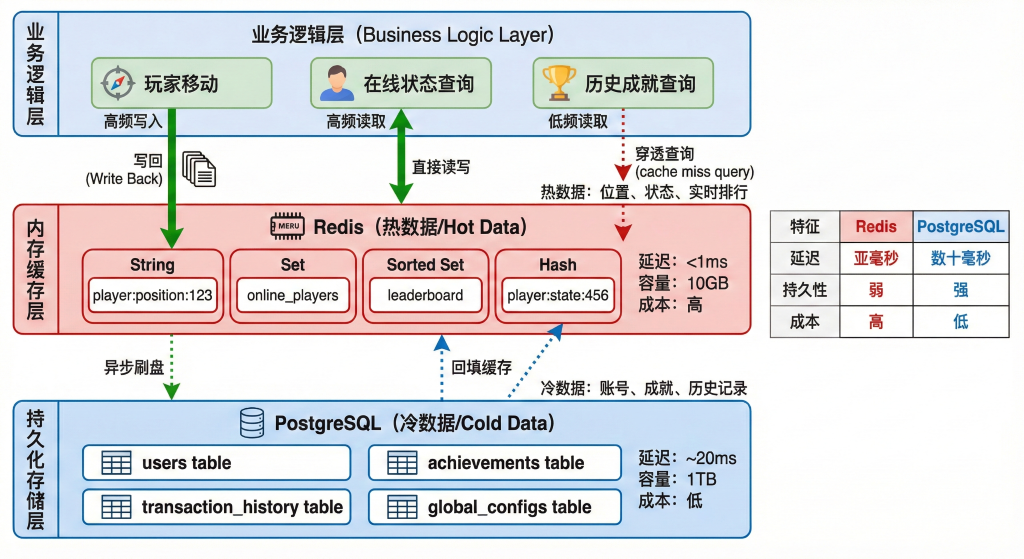
\includegraphics[width=1\linewidth]{figures/sec3/image3-7.png}
    \caption{Redis+PostgreSQL分层存储架构：热数据存内存保证低延迟，冷数据存磁盘保证持久性和低成本}
    \label{fig:redis-postgres}
\end{figure}

表\ref{tab:sync-strategy}总结了三种数据同步策略的特征与适用场景。在实际工程中，不同类型的数据会采用不同的同步策略，以在一致性、性能和成本之间取得最优平衡。

\begin{table}[h]
\centering
\caption{数据同步策略的特征与适用场景}
\label{tab:sync-strategy}
\begin{tabular}{p{3.5cm}p{4cm}p{5cm}}
\hline
\textbf{同步策略} & \textbf{一致性/性能} & \textbf{适用场景} \\
\hline
写穿（Write Through） & 强一致，写延迟高 & 金币交易、装备绑定等关键资产操作 \\
写回（Write Back） & 最终一致，写延迟低 & 玩家位置、临时状态等允许短时丢失的数据 \\
失效更新（Cache Aside） & 最终一致，读性能优 & 物品配置、技能描述等读多写少的静态数据 \\
\hline
\end{tabular}
\end{table}

在实际的游戏服务器中，不同的游戏操作会根据其数据特征选择不同的同步策略。玩家移动是最高频的操作，每秒可能触发数十次坐标更新，但丢失最近几秒的位置数据并不致命——玩家重新连接后客户端会立即上报当前位置，因此移动数据采用写回策略，先写入Redis保证低延迟响应，再由后台任务每隔数秒批量刷入持久存储。击杀与死亡事件虽然频率远低于移动，但它们直接影响排行榜和玩家战绩统计，属于不可丢失的关键事件，因此采用写穿策略，同步写入Redis排行榜和PostgreSQL战绩表，确保两层数据始终一致。金币获取同理——金币是玩家的核心资产，任何丢失都会引发投诉，必须采用写穿策略双写保障。而装备配置、技能参数等静态数据在游戏运行期间几乎不会变化，属于典型的读多写少场景，采用失效更新策略：首次读取时从数据库加载并缓存到Redis，后续读取直接命中缓存；只有在运营人员修改配置时才删除缓存，触发下次读取时重新加载。这种按数据特征选择同步策略的设计思路，是缓存分层架构从理论走向工程落地的关键一步。示例代码中各操作与缓存策略的具体对应关系及实现细节，请参见附录D。

这种分层存储架构不仅是技术实现的优化，更是成本与可靠性的工程权衡。Redis按内存容量计费，成本较高但性能极致；PostgreSQL按存储容量计费，成本低廉但延迟较高。通过将热数据和冷数据分离，可以在满足性能需求的前提下，将存储成本降低数倍。以一个10万在线玩家的游戏为例，如果所有数据都存储在Redis中，每个玩家100KB数据就需要约10GB内存，按云服务商报价计算可能需要数千元月费；而通过分层架构，只将关键热数据（如在线状态、当前位置）存储在Redis中，每玩家仅需1KB，总内存降至100MB，成本降低99\%，而大部分冷数据存储在便宜的PostgreSQL中。这种架构设计体现了云计算"按需使用、成本优化"的核心理念。

\subsubsection{性能验证：用可观测指标量化优化效果}

上述从连接池、对象池到缓存分层的优化设计，本质上都是为了在同一台物理服务器上争取更高的并发承载能力。然而，这些优化是否真正奏效，不能停留在理论分析和直觉判断的层面，而必须通过系统性的压力测试和性能监控来量化验证。只有建立了可观测的性能基线和瓶颈识别能力，才能科学地判断单机优化的边界在哪里，何时应该继续纵向优化，何时必须转向横向扩展。

性能验证的核心在于定义和测量关键指标。对于游戏服务器，最重要的三类指标是吞吐量、延迟分布和资源占用。吞吐量（Throughput）通常用QPS（Queries Per Second）或TPS（Transactions Per Second）来衡量，表示系统每秒能够处理的请求数量。对于我们的游戏服务器，可以测量每秒处理的玩家移动请求数、战斗计算数、状态同步广播数等。吞吐量反映了系统的整体承载能力，是评估优化效果最直观的指标。延迟分布（Latency Distribution）则关注每个请求从发起到收到响应的耗时。与平均延迟相比，P95和P99延迟（即95\%和99\%的请求在多长时间内完成）更能反映用户的真实体验。对于实时游戏，即使平均延迟只有10毫秒，如果P99延迟达到500毫秒，仍然会有1\%的玩家遭遇明显卡顿。资源占用（Resource Utilization）包括CPU使用率、内存占用、网络带宽消耗以及GC统计信息。这些指标帮助我们定位瓶颈所在：如果CPU使用率已达90\%但内存充足，说明瓶颈在计算能力；如果GC暂停频繁，说明内存分配模式需要优化；如果网络带宽打满，说明需要优化消息序列化或引入压缩。

为了量化优化效果，可以设计对比实验。首先，建立基准测试场景：模拟100个并发玩家，每个玩家每秒发送5次移动请求和1次战斗请求，持续运行5分钟，测量未优化版本的性能指标。在这个基准场景下，假设未引入连接池时，由于频繁建连和断连，系统吞吐量可能只有300 QPS，P99延迟达到800毫秒，CPU使用率60\%但大部分时间消耗在系统调用而非业务逻辑。引入数据库连接池后，吞吐量提升到1200 QPS，P99延迟降至150毫秒，因为握手开销大幅减少。进一步引入\texttt{sync.Pool}优化临时对象分配后，GC暂停时间从平均50毫秒降至10毫秒，P99延迟继续降至100毫秒，系统响应更加稳定。最后，引入Redis+PostgreSQL分层架构后，热数据访问延迟从平均20毫秒（访问磁盘数据库）降至1毫秒（访问内存缓存），吞吐量突破2000 QPS，P99延迟稳定在50毫秒以下。通过这样的对比实验，可以清楚地看到每项优化带来的性能提升，也能识别出当前的主要瓶颈。

更重要的是，性能验证帮助我们确定单机优化的边界。当继续增加并发玩家数到500人时，如果发现CPU使用率已达95\%，继续优化代码逻辑只能带来不到5\%的提升，这说明单机的计算能力已接近极限。此时，继续在单机上堆砌优化技巧的收益递减，性价比很低。相反，如果将系统拆分为多个服务实例，通过负载均衡分散请求，可以线性地提升承载能力。这种基于数据的决策判断，正是工程化思维的核心：不是凭感觉优化，而是通过可量化的指标识别瓶颈，评估投入产出比，科学地选择优化方向。当单机优化的边际效益低于横向扩展时，就是转向第四章分布式架构的信号。


\subsection{小结：从“单兵作战”到“军团指挥”}

本章系统性地解决了单机服务器在多人同图场景下的三大核心挑战，完成了从"能运行双人"到"稳定承载多人同图"的关键跨越。在并发组织能力层面，我们通过Goroutine和Channel建立了高效的任务拆解与协作机制，将顺序执行模型改造为可并发的流水线架构。Goroutine的轻量级特性使得"每连接一协程"的架构模式在资源消耗上成为可能，而Channel提供的消息传递机制则将网络I/O层和业务逻辑层有效解耦，使得I/O等待不再阻塞整体吞吐。在正确性保障层面，我们通过Mutex互斥锁机制解决了并发环境下的数据竞争问题，确保关键的游戏规则修改被收敛为原子操作，维护了多人同图场景下规则的确定性和可信度。通过合理设计锁的粒度，在全局锁、区域锁和对象锁之间取得平衡，既保证了正确性又最大化了并发度。在资源效率层面，我们通过连接池复用TCP连接，通过\texttt{sync.Pool}复用临时对象，通过Redis加PostgreSQL的分层架构将数据访问路径优化到极致，在性能、成本和可靠性之间找到了合理的权衡点。

从云计算能力曲线的视角看，本章完成的是纵向优化阶段（Scale Up）的全部任务。我们把单机的并发潜力和资源利用率压榨到了可观测的极限，建立了清晰的性能基线和瓶颈识别能力。通过压力测试和性能监控，我们可以量化地回答：在当前的硬件配置下，单机能够支撑多少并发玩家，每种优化带来了多大的性能提升，以及当前的主要瓶颈在哪里。更重要的是，我们通过性能指标可以科学地判断：当单机CPU使用率已达90\%以上，继续优化代码带来的提升已不足10\%时，纵向优化的边际收益递减，性价比降低。此时，继续在单机上堆砌优化技巧已无法从根本上突破承载能力的天花板，必须转向横向扩展（Scale Out）的分布式架构。

在第四章中，我们将跨越单机边界，进入分布式阶段。此时的核心矛盾将从"如何在单机内高效并发"转变为"如何在多机间保持状态一致"。当游戏世界从单张地图扩展为多张地图、从单个服务实例扩展为多个服务集群时，新的挑战随之而来：跨地图边界的玩家如何感知彼此、跨服战斗的裁决权归属于谁、玩家在不同服务器间迁移时如何保证状态的连续性和一致性。这些问题的本质是分布式系统中的经典难题：数据的跨节点同步、操作的全局顺序保证、以及故障场景下的可用性维护。我们将通过服务拆分、一致性协议和云原生部署等手段，完成从单机优化到分布式协同的架构演进，这正是云计算从"资源可获得"走向"服务可规模化"的关键跨越。




% \subsection{敞开大门：让服务器迎接成千上万的玩家}
% % 具体的实现过程 

% \paragraph{本节目标} 基于 3.1 节确立的技术逻辑框架，围绕 Go 语言并发与高性能网络库优势，探索 “连接池 + 缓存分层” 优化方案，助力突破单机性能瓶颈，提升服务承载能力。
% \paragraph{写作建议}
% \begin{enumerate}
%     \item 基于Go的驱动的优化
%     \paragraph{连接池构建} 基于 3.1 中奠定的技术基础，进一步利用 Go 标准库与sync.Pool，设计协程安全的 TCP 连接池，实现连接复用与生命周期管理。
%     \paragraph{缓存分层架构} 结合go-redis与gorm，分别处理高频与低频数据，在 3.1 逻辑的延伸下，优化读写效率与数据库负载。其中，高频数据指的是在游戏运行过程中被频繁读取或修改的数据，例如玩家当前的游戏在线状态、实时积分、正在进行的游戏对局数据等，这些数据的访问频率极高，将其存储在go-redis缓存中，能快速响应请求，减少数据库压力。而低频数据则是访问频率较低、更新不频繁的数据，像玩家的历史成就记录、注册信息、游戏角色的基础属性配置等，这类数据更适合使用gorm操作pgsql持久化数据库进行存储和管理，既能保证数据的安全性和完整性，又不会因频繁读写影响数据库性能。
%     \item 测量性能。比较单机和并发优化后的单机的承载能力，模拟高并发场景进行压测，监控关键指标并优化系统性能，通过实践验证 3.1 中理论逻辑的实际可行性与优化方向。
% \end{enumerate}



\newpage

% \section*{附录：第三章核心技术索引}

% \newpage
\section{第四章\ 从单机到多机：分布式游戏世界的地基}\label{sec:chapter4}

在第三章中，我们完成了从"双人原型"到"单服高并发战场"的跨越：通过 Goroutine 并发调度、细粒度锁和连接池等技术，将一台服务器的计算与网络资源压榨到了接近单机物理极限。这一阶段的核心问题是：如何在一台机器内部，让尽可能多的玩家同时在线、同时战斗，而不会因为锁冲突严重或调度阻塞而拖垮整台服务器。经过第三章的系统优化，我们成功地让单台服务器从只能支撑几十个玩家的原型状态，提升到了可以稳定承载数百甚至上千玩家同时对战的生产级水平。

然而，当这些问题被基本解决之后，游戏世界真正的瓶颈就从"并发正确性"悄然转移到了"整体容量"。这种转移并非突然发生，而是一个渐进的过程。起初，我们可能会注意到服务器的 CPU 使用率在高峰时段接近百分之八十，偶尔会出现短暂的响应延迟；随着玩家数量继续增长，这种延迟变得越来越频繁，数据库查询开始排队，网络带宽也逐渐饱和。即使我们继续优化代码——比如进一步细化锁的粒度、优化数据结构、减少不必要的内存分配——这些改进带来的收益也会越来越小。最终，我们不得不面对一个残酷的事实：一台物理机器，无论优化得多么精细，最终都只能承载有限数量的玩家。

这个"有限数量"的具体数值取决于多个因素：服务器的硬件配置、游戏逻辑的复杂度、玩家的活跃程度等。对于我们在第二章和第三章中构建的对战游戏服务器来说，假设使用一台配置了 16 核 CPU、64GB 内存的服务器，在玩家密集进行战斗的情况下，当在线人数接近 2000 时，系统的响应延迟就会开始显著上升；而当人数突破 3000 时，服务器很可能会因为资源耗尽而出现严重的性能下降，甚至崩溃。这个数字看起来已经不小，但对于一款希望服务更大规模玩家群体的游戏来说，显然还远远不够。


随着玩家数量增长、活动内容增多、世界版图扩张，一个自然的问题随之出现：如果再加几台服务器，让它们一起分担压力，会不会更好？这个想法看起来直截了当——既然一台服务器能承载 2000 人，那么两台服务器不就能承载 4000 人，十台服务器就能承载 20000 人了吗？从纯粹的容量角度看，这个逻辑确实成立。但是，当我们真正开始思考如何把这个想法落地时，就会发现"加机器"远没有想象中那么简单。

首先，玩家数据该怎么办？在单机环境下，所有玩家的账号信息、角色属性、战斗记录都存储在同一个数据库中，应用服务器可以随时查询任何一个玩家的数据。但现在有了多台游戏服务器，是让每台服务器都连接同一个数据库，还是为每台服务器配备独立的数据库？如果所有服务器共享一个数据库，那么数据库本身就会成为新的瓶颈——它需要同时响应所有服务器的查询请求，压力会比单机时代更大。如果为每台服务器配备独立的数据库，那么玩家 A 的数据存在服务器 1 的数据库中，玩家 B 的数据存在服务器 2 的数据库中，当需要查询全服排行榜或者统计全服在线人数时，又该如何处理？

其次，玩家该如何被分配到不同的服务器？在单机时代，所有玩家登录后自动进入同一个服务器，不存在选择的问题。但现在有了多台服务器，我们需要在玩家登录时为他们选择一台服务器。最简单的方式是让玩家自己选择，就像传统网络游戏中的"选区"——玩家在登录时看到一个服务器列表，自己决定进入哪一个。但这种方式很容易导致负载不均：一些服务器因为各种原因（比如开服时间早、口碑好）变得人满为患，而另一些服务器则门可罗雀。更理想的方式是由系统自动分配，根据各服务器的实时负载情况，把新玩家引导到相对空闲的服务器上。但这就需要一套负载监控和调度机制，并且要确保这套机制本身不会成为新的性能瓶颈。

第三，不同服务器上的玩家能否互动？在单机时代，所有玩家都在同一个游戏世界中，彼此可以自由交互——组队、对战、交易等。但当玩家被分散到多台服务器上时，这种互动就变得复杂了。如果服务器 1 的玩家想要挑战服务器 2 的玩家，战斗逻辑该在哪里执行？是在服务器 1 上，还是在服务器 2 上，还是需要一个专门的"裁判服务器"？如果战斗结果在服务器 1 上计算出来，如何确保服务器 2 也能及时、准确地获取这个结果，并更新本地玩家的数据？如果网络出现延迟或中断，导致两台服务器对同一场战斗的结果产生了分歧，又该如何处理？



\begin{figure}[H]
    \centering
    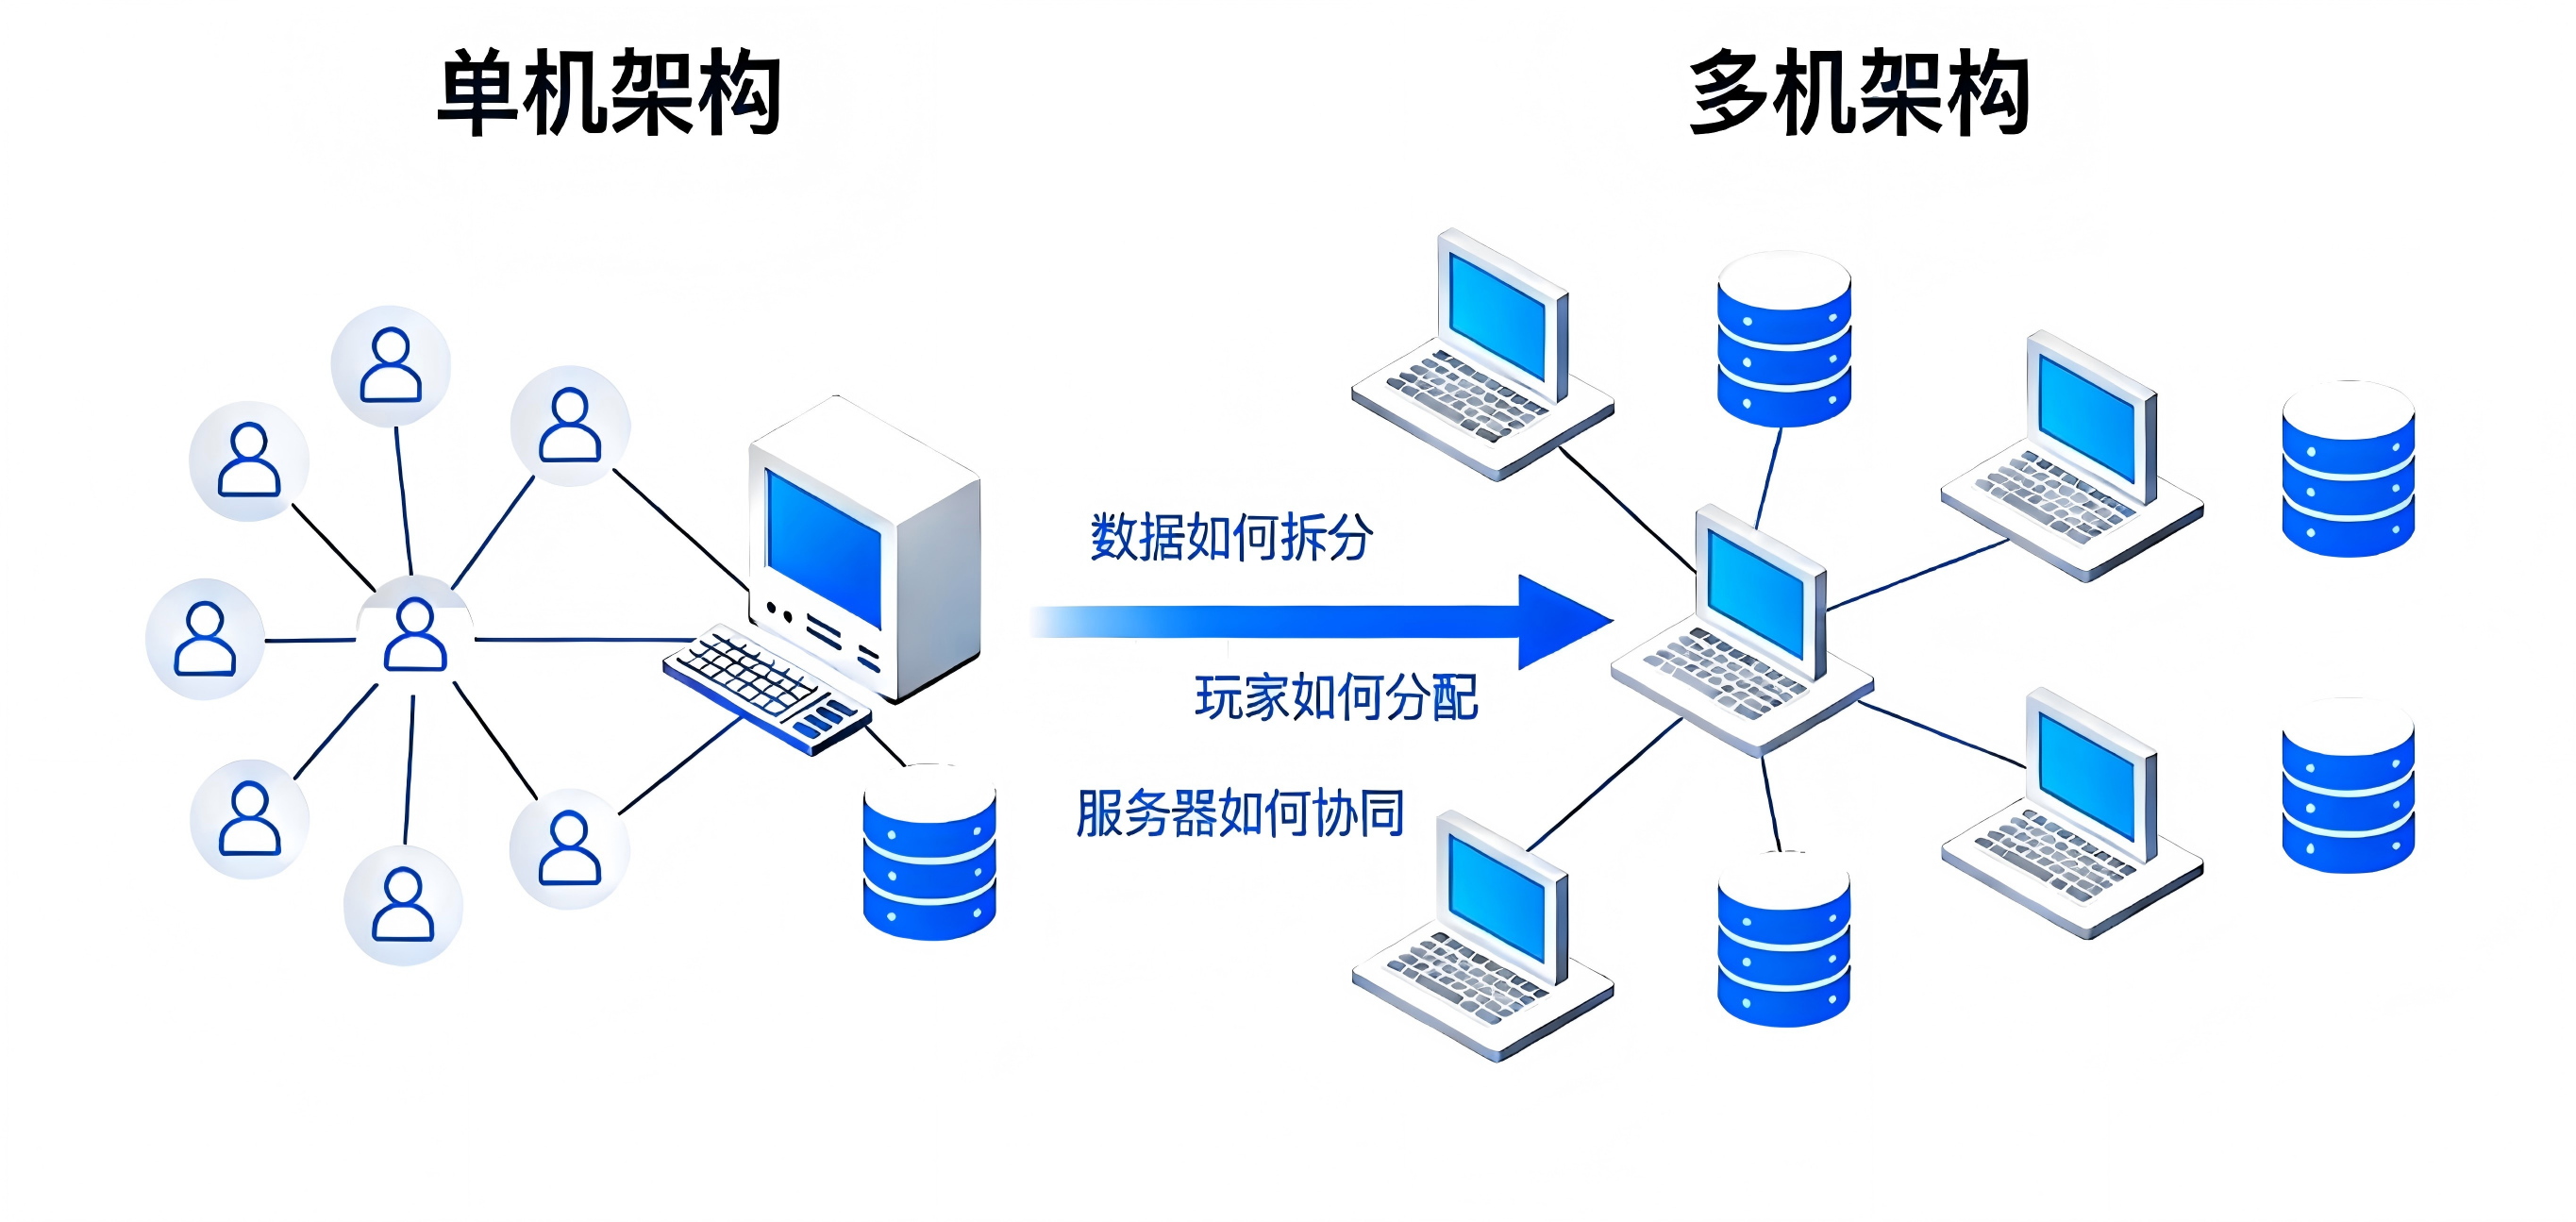
\includegraphics[width=1\linewidth]{figures/sec4/4-1.png}
    % 图片描述：展示从单机到多机架构的演进示意图
    % 左侧：单机架构，一个应用服务器连接一个数据库，所有玩家连接到这一个服务器
    % 右侧：多机架构，多个应用服务器，可能共享数据库或使用独立数据库
    % 用箭头标注出三个核心问题：数据如何拆分、玩家如何分配、服务器如何协同
    \caption{从单机到多机架构的演进与核心挑战}
    \label{fig:single_to_multi_server}
\end{figure}

这三个问题——数据放在哪里、玩家如何分配、不同服务器如何协同——构成了从单机到多机演进过程中必须解决的核心挑战。它们彼此关联、相互影响，形成了一个复杂的技术网络。数据的存放方式会影响查询效率，进而影响负载均衡的策略；负载均衡的效果会影响各服务器的压力分布，进而影响跨服交互的设计；跨服交互的实现方式又会对数据一致性提出新的要求，进而影响数据存储的架构选择。这就是为什么"加机器"这个看似简单的想法，在实际落地时会引发一系列连锁反应。

更深层次地说，从单机到多机的演进，本质上是从"集中式架构"到"分布式架构"的转变。在集中式架构中，所有的状态、所有的决策、所有的数据都集中在一个地方，系统的行为是确定的、可预测的。但在分布式架构中，状态被分散到多台机器上，每台机器都有自己的"局部视角"，它们需要通过网络通信来协调彼此的行为。网络通信是不可靠的——消息可能延迟、可能丢失、可能乱序到达；机器也是不可靠的——随时可能崩溃、重启、断网。在这样的环境下，如何确保系统整体上仍然能够正确、一致地运行，就成了分布式系统设计的核心挑战。

本章的目标，就是带领大家系统地理解和解决这些挑战。我们将从最基础、也是最关键的三个问题出发，将整章拆分为三个循序渐进的小节。第一节，我们会详细讲解"如何拆分数据"，介绍数据库分片的核心概念、常见策略，以及分片后会遇到的查询和事务问题；第二节，我们会深入探讨"如何分配玩家与负载"，从最简单的轮询策略开始，逐步引入动态调度、健康检查等机制，帮助大家理解负载均衡的完整体系；第三节，我们会通过一个具体的"跨服擂台"案例，把前两节学到的抽象概念织进一个完整的玩法场景之中，让大家亲身体验分布式环境下的跨服交互是如何设计和实现的。

通过这三个小节的学习，大家不仅能够掌握分布式游戏服务器的基础架构技术，更重要的是，能够建立起一套分布式系统思维——学会在设计任何涉及多台机器协同工作的系统时，自觉地去思考数据如何分布、负载如何均衡、节点如何协调这些根本性的问题。这种思维方式，不仅适用于游戏服务器，也适用于任何大规模的分布式应用系统。


\subsection{数据库分片：突破单机存储的容量上限}

回顾第三章，我们为单机服务器建立了Redis+PostgreSQL的分层存储架构：Redis承载高频热数据（在线状态、实时位置、排行榜），PostgreSQL持久化低频冷数据（账户信息、历史战绩、装备配置），两者通过写穿、写回、失效更新三种策略协同工作。在单机阶段，这套架构运行良好——一个Redis实例加一个PostgreSQL实例，足以支撑数百到数千名玩家的并发访问。

然而，当玩家规模从数千增长到数万乃至数十万时，这套单机数据层会在两个方向上同时触及天花板：PostgreSQL的磁盘I/O和连接数达到上限，查询延迟急剧恶化；Redis的内存容量不足以容纳所有在线玩家的热数据，开始频繁淘汰缓存导致穿透到数据库。此时，单纯的纵向扩展（换更大的机器）已经无法解决问题，我们必须将数据层从单实例拆分为多实例——这就是数据库分片的由来。本节将首先讨论PostgreSQL的分片策略，随后在本小节末尾说明Redis缓存层如何同步完成分布式演进。

当游戏还停留在单机阶段时，数据层的世界是简单而直观的：所有玩家的账号、角色、战斗记录，都躺在同一个数据库实例里，应用服务器只要连上这一个地址，就可以查到任何一个玩家的所有信息。在这个阶段，开发者更多关注的是"如何把这一个数据库调优到足够扛打"——加索引、调连接池、做缓存；但随着玩家规模上升，这个"一个数据库"慢慢变成了游戏世界里最脆弱的一块地基。

在深入讨论每一个具体问题之前，有必要先建立一个整体的架构视图，
下图展示了本节所涉及的数据分片体系的全貌。
整个体系自上而下分为三个层次：最上层是游戏应用服务器，它是所有数据库请求的发起方；
中间层是分片路由层，它是整个分片体系的神经中枢，负责接收来自应用服务器的请求，
根据请求中携带的玩家 ID 和预先配置的分片规则，计算出目标分片编号，
再将请求精准转发到对应的数据库实例；最下层是由多个 PostgreSQL 分片实例组成的存储层，
每个分片只负责全量玩家数据的一个子集，各分片之间相互独立，互不干扰。
与 PostgreSQL 分片层并列运行的，是 Redis 缓存集群，
它以相同的分片逻辑将热数据键空间拆分到多个 Redis 节点上，
承载在线状态、实时位置、排行榜片段等高频访问数据，与冷数据层共同构成完整的分布式数据层。

\begin{figure}[H]
    \centering
    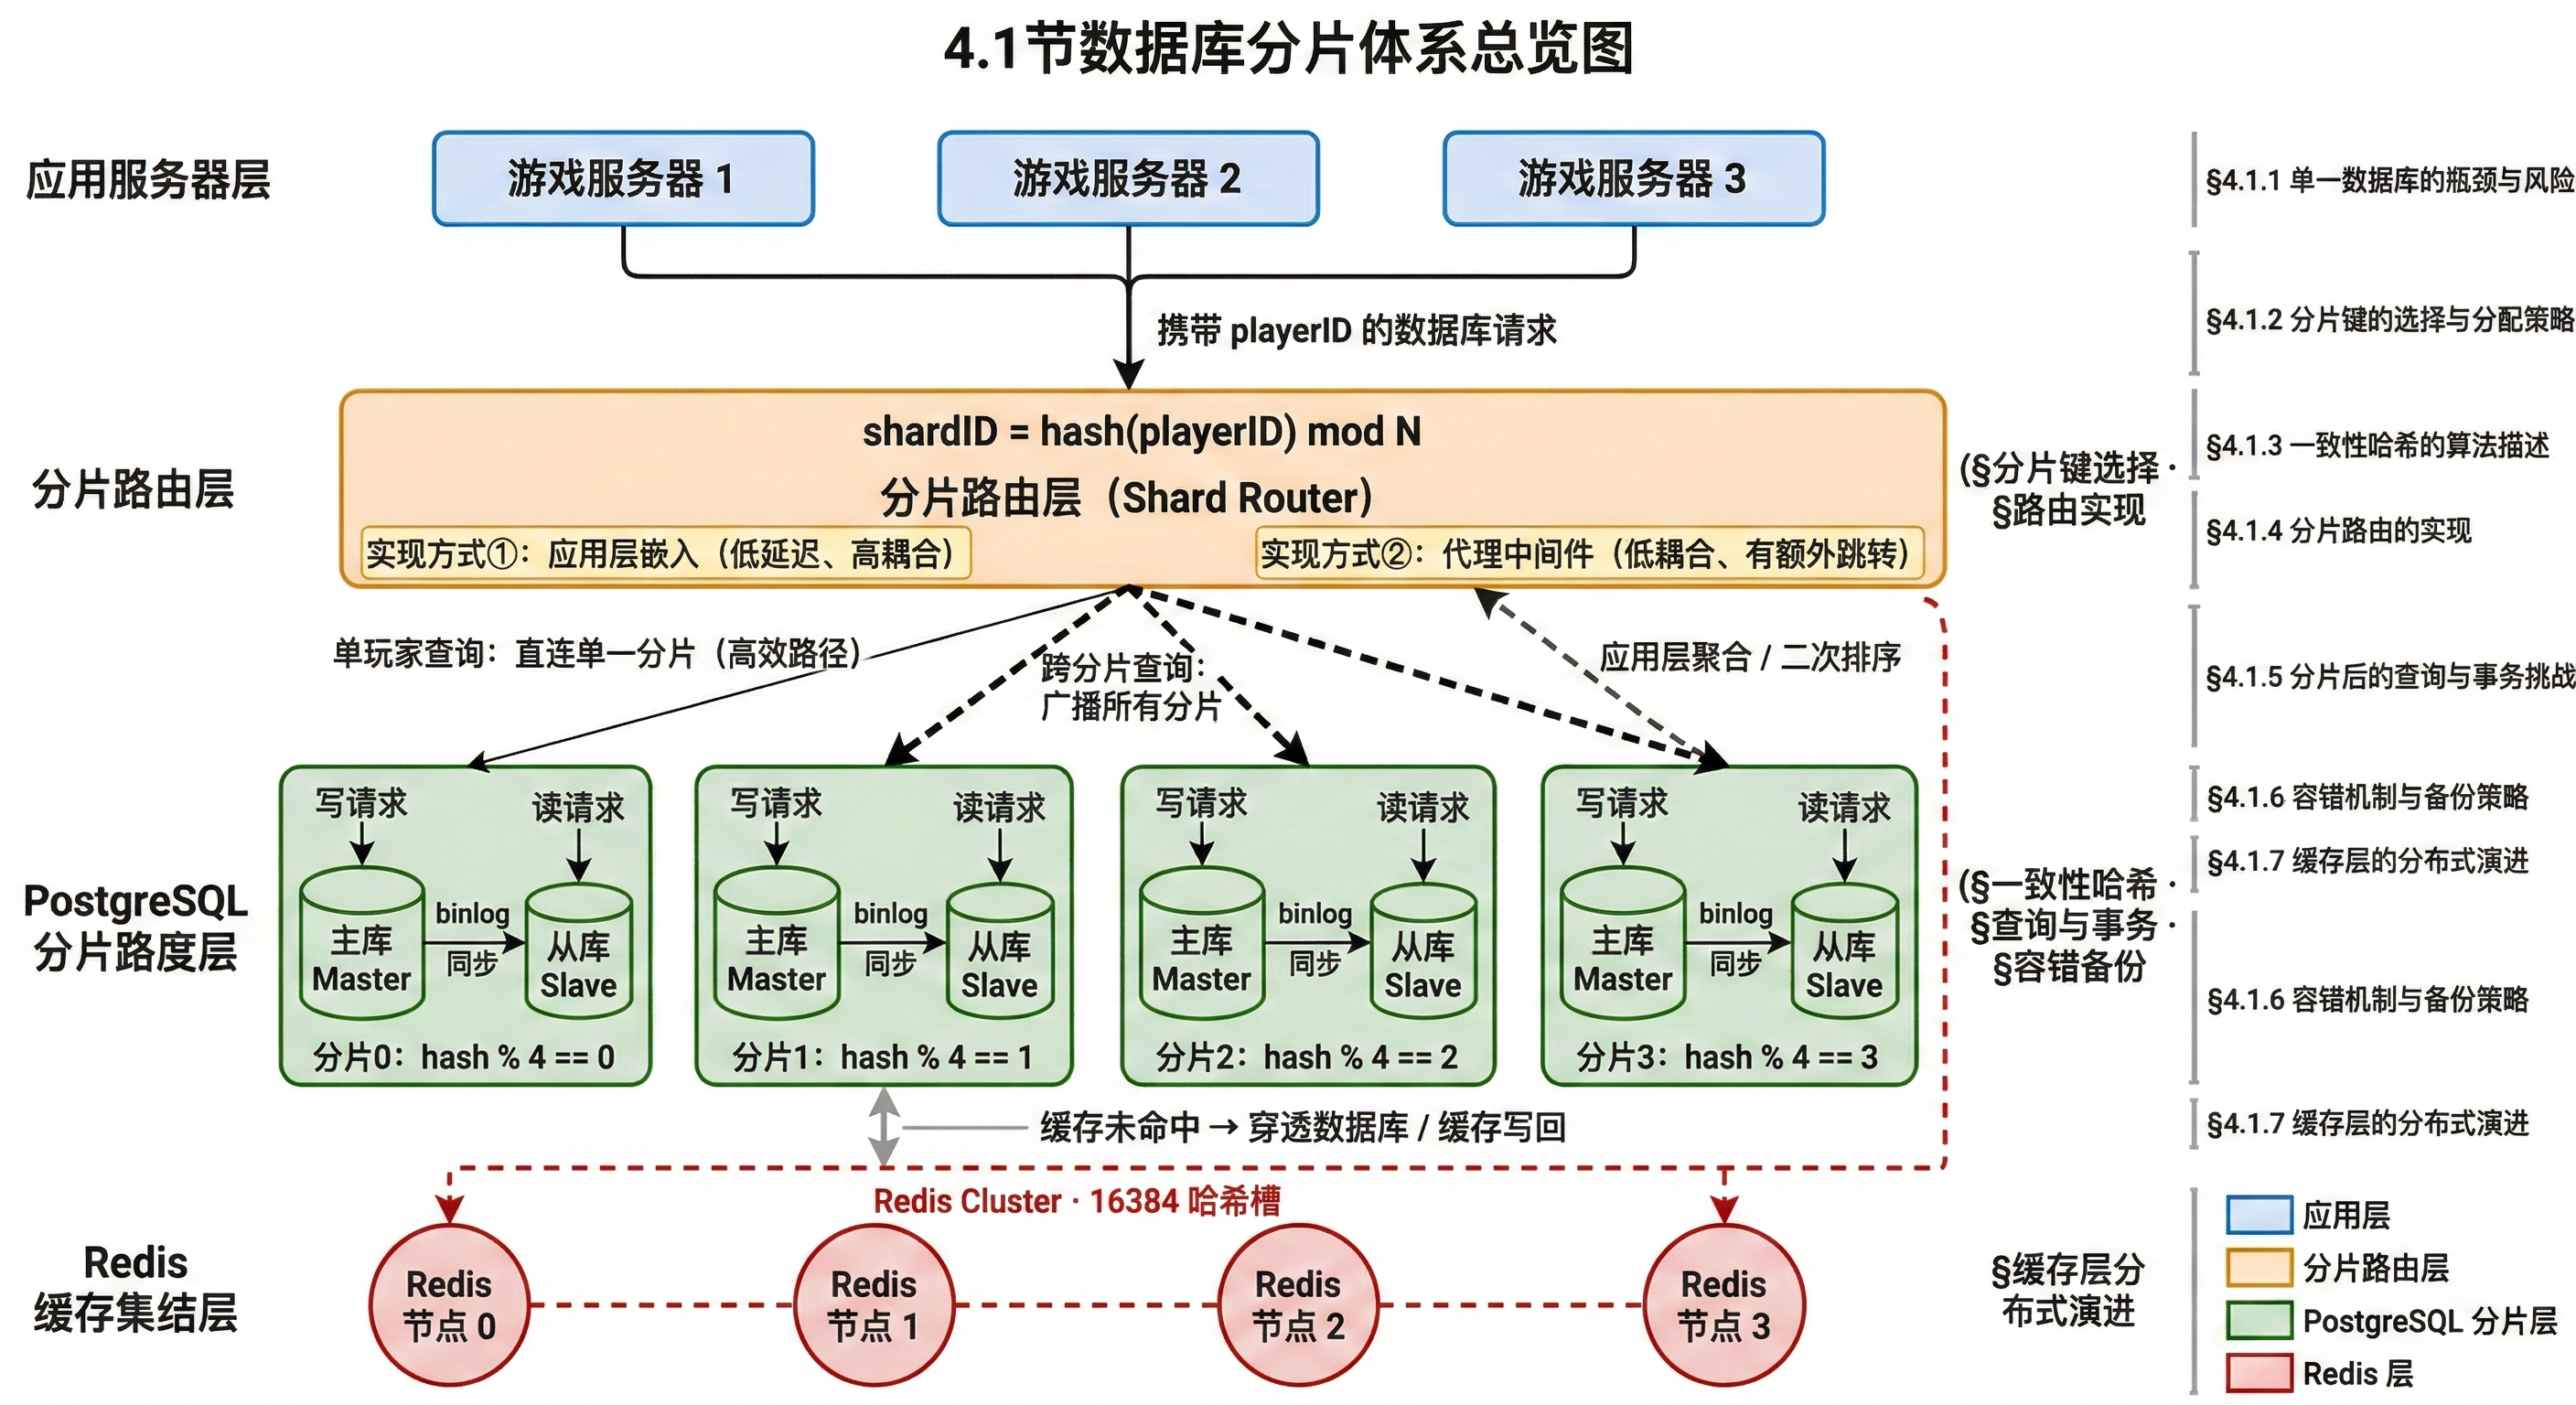
\includegraphics[width=1\linewidth]{figures/sec4/4-1-1.png}
    \caption{数据库分片体系总览}
\end{figure}

这张图揭示了整个分片体系的两条核心请求链路。
第一条是单玩家查询链路：请求携带玩家 ID 进入路由层，
路由层经过一次哈希计算便能唯一确定目标分片，请求直达单个数据库节点，
全程无需跨节点协调，这是分片架构在正常访问路径上高效运作的根本原因。
第二条是跨分片链路：当查询不能通过分片键唯一定位时——
例如全服战力排行榜需要聚合所有分片的数据——
路由层必须将请求广播到全部分片，由各分片分别执行子查询，
再由应用层将各分片的局部结果合并排序后返回最终答案；
分布式事务同样属于跨分片链路的范畴，需要通过两阶段提交协议或业务层异步化来保障操作的原子性。
这两条链路的效率差异，正是本节反复强调"尽量将查询限制在单一分片内"这一设计原则的根源。

本节各小节的讨论便是沿着这张图从上到下、由浅入深地逐层展开的。
首先从单一数据库所面临的硬件天花板和单点故障风险出发，说明为什么必须走向水平拆分；随后讨论分片键的选择与三种分配策略——范围分片、哈希分片、一致性哈希——之间的权衡，
以及一致性哈希如何通过哈希环和虚拟节点将扩容时的数据迁移量控制在局部区间；接着说明路由层的两种实现方式，即应用层嵌入路由逻辑与引入代理中间件各自的适用场景；
然后面对分片后不可回避的两类技术难题，即跨分片聚合查询的效率损耗，以及跨分片事务的一致性保障与业务层规避策略；
再之后讨论每个分片内部的主从复制架构、定期备份机制与恢复演练，构建完整的容错体系；最后将视角切换到 Redis 缓存集群，说明热数据层如何完成与冷数据层对称的分布式演进，补全整个数据层的水平扩展图景。
%理解了这张总览图中各组件的角色与两条链路的走向，再阅读后续各小节的技术细节，便能始终清楚自己在整个分片体系中所处的位置。


\subsubsection{单一数据库的瓶颈与风险}

从最直观的角度看，单一数据库的瓶颈首先体现在硬件资源的天花板上。一台数据库服务器的 CPU 核心数、内存容量、磁盘 I/O 吞吐率都是有限的，当并发查询请求超过这些硬件资源所能承载的上限时，系统必然出现性能下降。可以想象这样一个场景：新版本上线，大量玩家同时登录、创建角色、领取奖励，这些操作最后都会汇聚到同一个数据库。一开始只是响应时间从正常的 50 毫秒逐渐攀升到 200 毫秒，玩家可能还察觉不到明显差异；但随着负载继续增加，响应时间可能突破 1 秒甚至更长，出现间歇性超时，部分玩家会看到"网络连接失败"的提示；最严重的情况下，数据库会直接触发过载保护机制，拒绝接受新的连接请求，导致大量玩家无法登录。

即使通过垂直扩展——也就是给这台机器加更多的 CPU、更大的内存——能够在一定程度上缓解压力，这条路终归是有尽头的。一台配置了 64 核 CPU、512GB 内存的高端数据库服务器，成本可能是普通服务器的十倍甚至更高，但性能提升往往达不到十倍。更关键的是，单台机器的物理极限也不可能无限突破：内存总线带宽、磁盘 I/O 吞吐量、网络接口速度都有上限，当这些指标逼近硬件极限时，再怎么堆钱也无法继续提升。

更深层的问题在于风险集中。当所有玩家的核心数据都存放在同一台数据库上时，这台机器的任何故障都会演化为全局灾难。硬盘损坏、网络中断、操作系统崩溃，任何一个环节出问题，都意味着整个游戏世界暂时失去了"记忆中枢"。虽然可以通过定期备份来降低数据永久丢失的风险，但备份无法解决实时可用性的问题——即使我们有昨天晚上的完整备份，当数据库在今天中午崩溃时，从发现故障、启动恢复流程、重新加载数据到服务恢复，整个过程可能需要数小时甚至更长时间，这对于一个需要 24 小时不间断运行的游戏服务来说是不可接受的。

从这两个角度出发，数据库拆分的核心动机便呼之欲出：通过将数据分散存储到多台独立的数据库实例上，一方面可以突破单机硬件资源的天花板，实现存储容量和查询吞吐量的水平扩展；另一方面，可以将风险分散开来，使得某一台数据库的故障只影响其所负责的那一部分玩家，而不会拖垮整个游戏世界。在分布式系统的术语中，这种将数据按照某种规则拆分到多台机器上的技术，被称为"数据库分片"（Database Sharding）。

\begin{figure}[htbp]
    \centering
    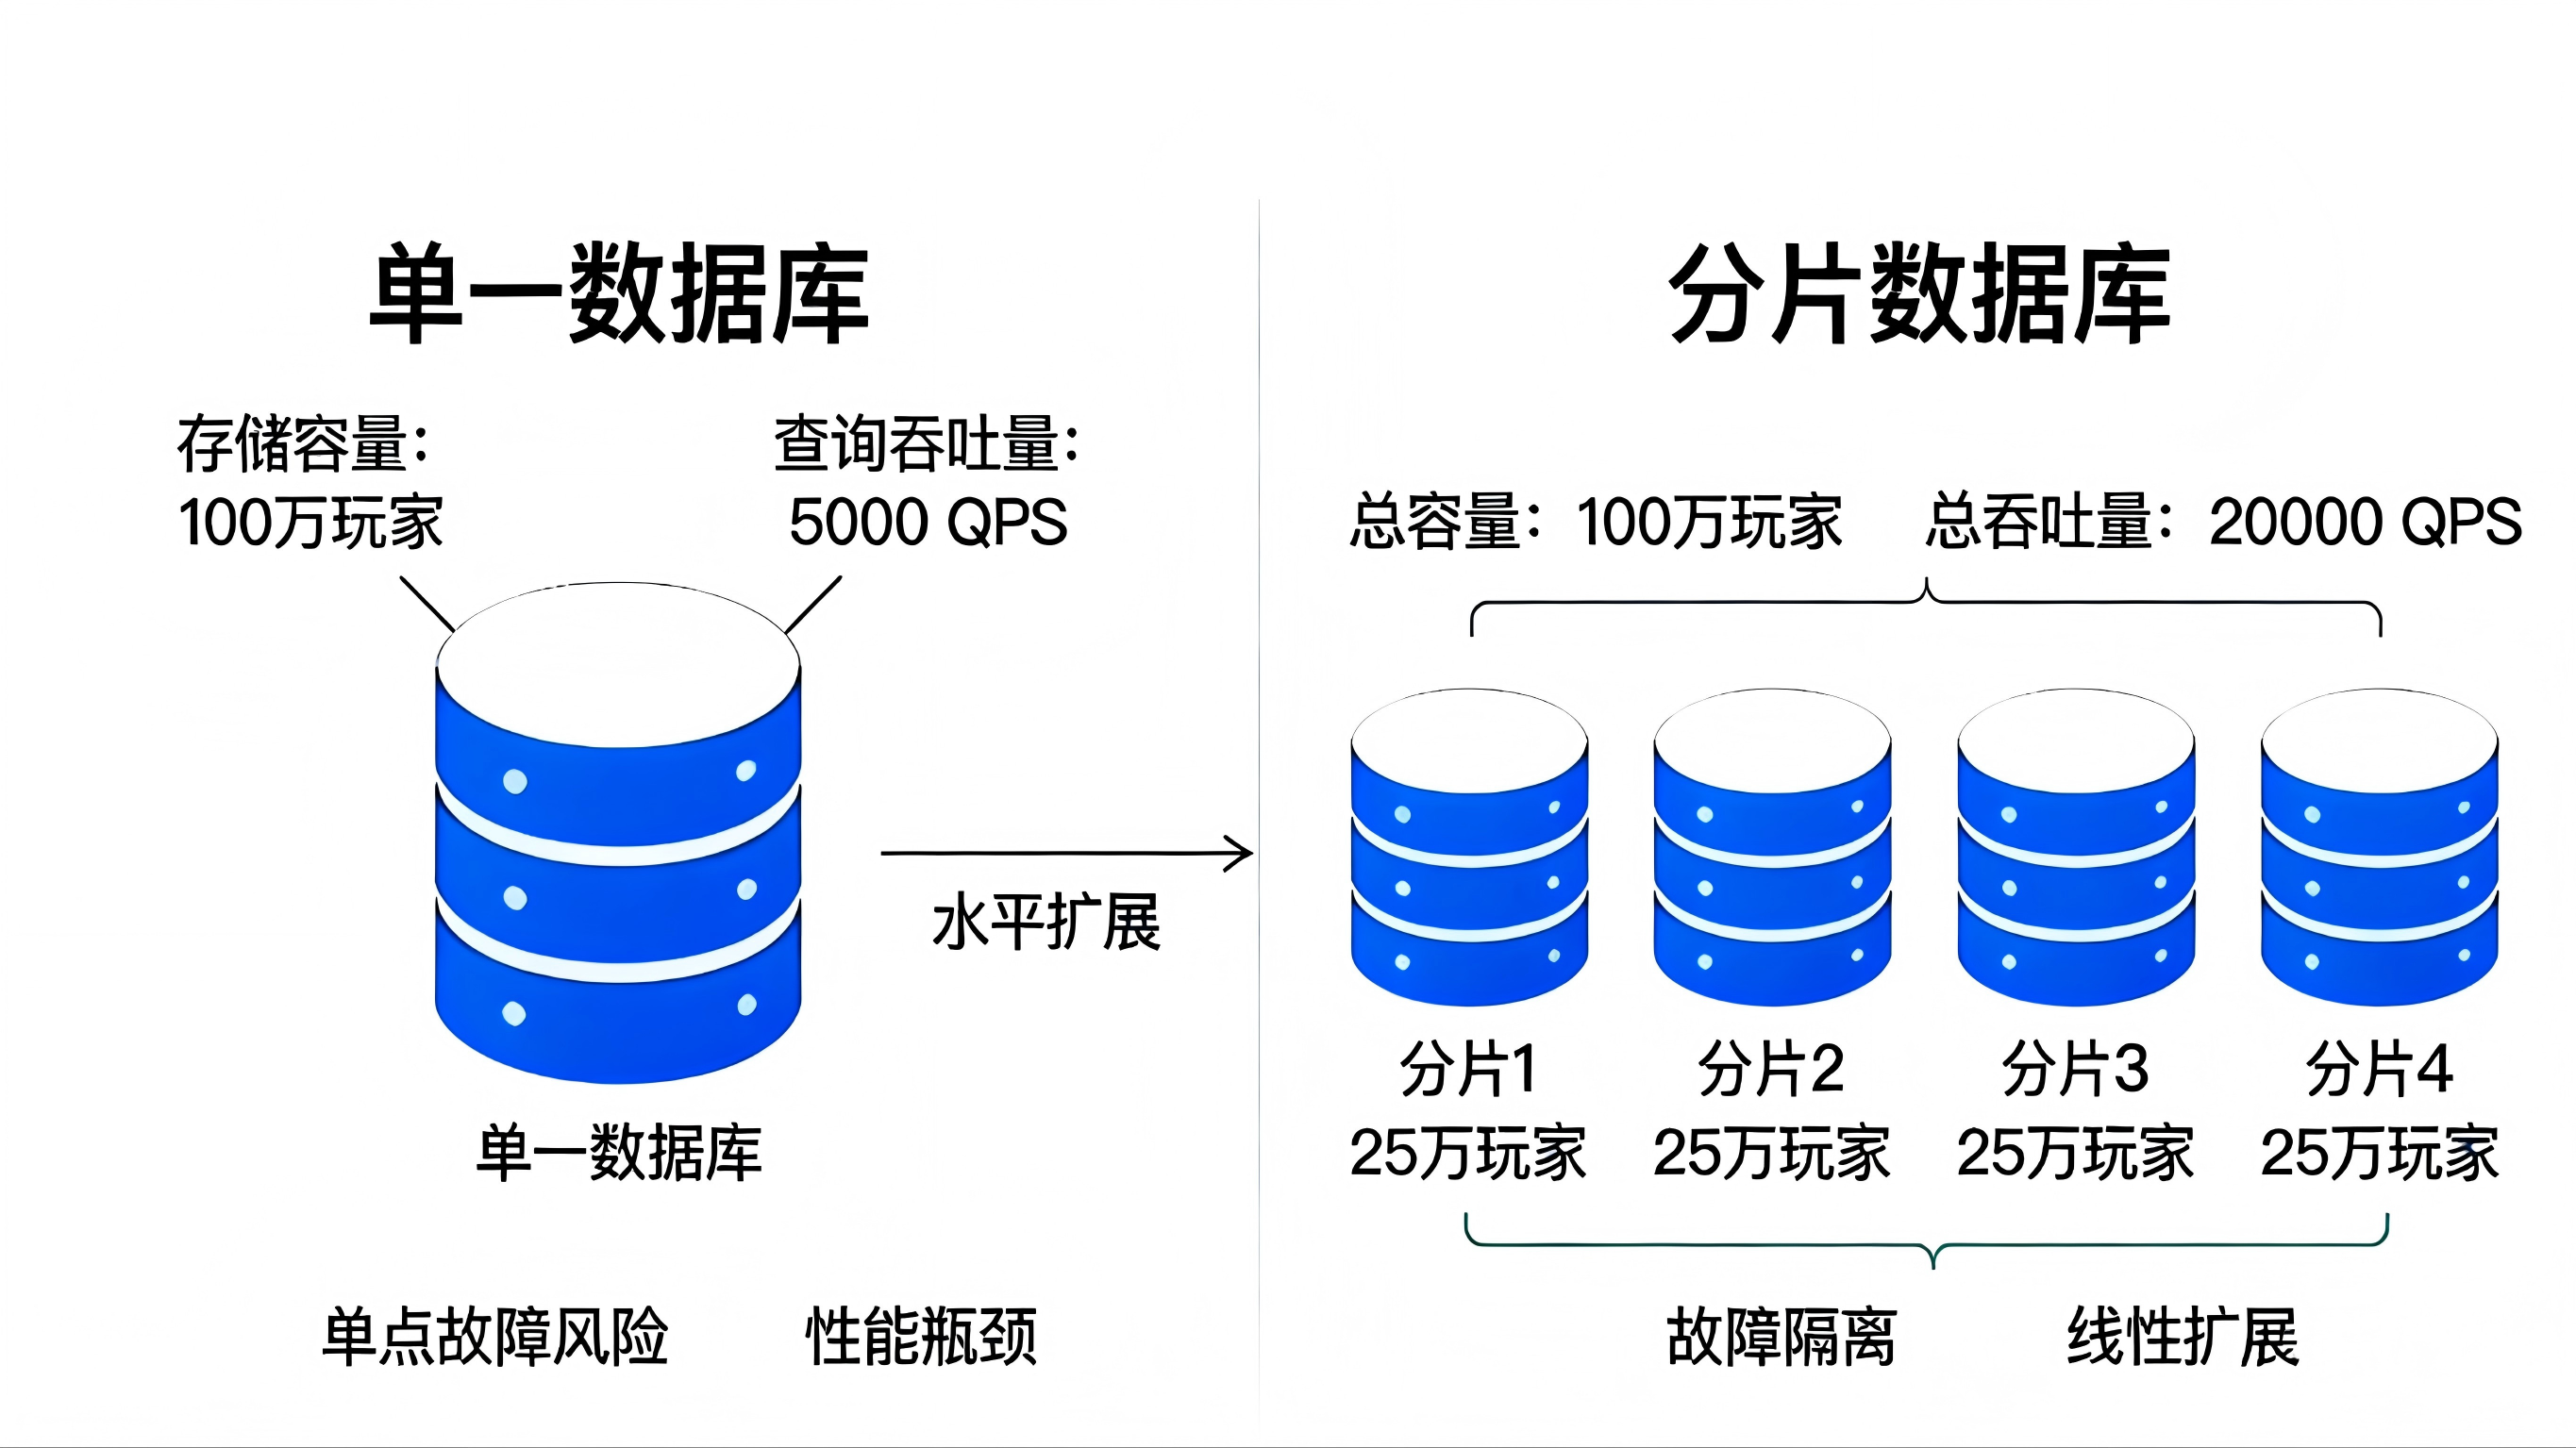
\includegraphics[width=1\linewidth]{figures/sec4/4-2.png}
    % 图片描述：单一数据库vs分片数据库的对比示意图
    % 左侧：单一数据库场景
    %   - 一个大的圆柱形数据库图标，标注"单一数据库"
    %   - 上方标注"存储容量：100万玩家"、"查询吞吐量：5000 QPS"
    %   - 下方用红色警告图标标注"单点故障风险"、"性能瓶颈"
    % 右侧：分片数据库场景（4个分片）
    %   - 四个较小的圆柱形数据库图标并排，分别标注"分片1"、"分片2"、"分片3"、"分片4"
    %   - 每个分片下方标注"25万玩家"
    %   - 上方汇总标注"总容量：100万玩家"、"总吞吐量：20000 QPS"
    %   - 下方用绿色对勾标注"故障隔离"、"线性扩展"
    % 中间用箭头连接，箭头上标注"水平扩展"
    % 所有文字使用简体中文，采用黑色粗体无衬线字体
    \caption{单一数据库与分片数据库的容量与风险对比}
    \label{fig:database_sharding_comparison}
\end{figure}

\subsubsection{分片键的选择与分配策略}

要理解数据库分片，需要先明确一个核心概念：分片键（Sharding Key）。分片键是用来决定某一条数据应该被分配到哪个数据库实例的关键字段。在游戏服务器的场景下，最自然的选择是以玩家 ID 作为分片键。原因很简单：首先，玩家 ID 在整个系统中是唯一的，每个玩家对应一个固定的 ID，这个 ID 在玩家整个生命周期内都不会改变，不会出现像昵称那样可能被修改的情况；其次，游戏中的绝大多数查询操作都是围绕玩家 ID 展开的——查询某个玩家的角色信息、战斗记录、背包物品等，都需要先知道玩家 ID。如果用玩家 ID 作为分片键，那么查询单个玩家的数据时，只需要根据 ID 定位到一个具体的数据库实例，不需要在多个实例之间查找。

确定了用玩家 ID 作为分片键之后，接下来需要设计具体的分配规则。这个规则需要回答一个简单但关键的问题：给定一个玩家 ID，它的数据应该存放在哪个数据库实例中？不同的分配规则会带来不同的特性和权衡，我们逐一分析三种常见的方案。

第一种方案是范围分片（Range-based Sharding）。这是最直观的一种方式：按照玩家 ID 的数值范围来划分数据。假设我们有三个数据库实例，可以这样分配：ID 从 1 到 1,000,000 的玩家存放在第一个数据库（分片 0），ID 从 1,000,001 到 2,000,000 的存放在第二个数据库（分片 1），ID 从 2,000,001 以上的存放在第三个数据库（分片 2）。这种方式的优点在于规则简单明了，容易理解和管理。当需要查询某个玩家的数据时，只需要简单地判断 ID 落在哪个区间即可。而且，如果需要扩容，只需要调整最后一个区间的边界，新增一个数据库实例来承接新的 ID 范围即可。

但范围分片也有一个明显的隐患——负载热点问题。如果玩家注册在时间上非常集中，比如游戏刚上线或举办大型活动期间，短时间内会有大量新玩家涌入，他们会被连续分配到相邻的 ID 区间。假设在一周内新注册了 50 万玩家，他们的 ID 都落在 2,000,001 到 2,500,000 这个范围内，全部被分配到分片 2。而这些新玩家往往是最活跃的——频繁登录、进行战斗、完成任务——导致分片 2 的负载远高于其他分片。这就像是一个不断向右延伸的队列，最右边的那一块总是最拥挤的。

% \begin{figure}[htbp]
%     \centering
%     % 图片描述：范围分片的热点问题示意图
%     % 横轴代表玩家ID范围（0到3,000,000），纵轴代表负载强度
%     % 三个区间分别用不同颜色柱状图表示：
%     %   - 分片0（ID 1-1,000,000）：绿色柱，高度较低，标注"老玩家，活跃度低"
%     %   - 分片1（ID 1,000,001-2,000,000）：黄色柱，高度中等，标注"中期玩家，活跃度中等"
%     %   - 分片2（ID 2,000,001以上）：红色柱，高度很高，标注"新玩家，活跃度高，形成热点"
%     % 在分片2上方标注红色警告标志和文字"负载热点"
%     % 所有文字使用简体中文
%     \caption{范围分片可能导致的负载热点问题}
%     \label{fig:range_sharding_hotspot}
% \end{figure}

为了避免这个问题，第二种方案是哈希分片（Hash-based Sharding）。具体做法是：对每个玩家 ID 执行一个固定的哈希运算，将结果对数据库实例数量取模，根据余数来决定数据存放的位置。用伪代码表示如下：

\begin{tcolorbox}[title=哈希分片的路由计算]
\begin{lstlisting}[
    language=go,
    basicstyle=\ttfamily\footnotesize,
    aboveskip=0pt, belowskip=0pt,
    lineskip=-1pt,
    commentstyle=\color{gray},
    keywordstyle=\color{blue}\bfseries,
    breaklines=true
]
// 假设有4个数据库分片
const numShards = 4

// 根据玩家ID计算目标分片
func getShardID(playerID int) int {
    // 对玩家ID执行哈希运算（这里用简单的取模代替）
    hash := playerID
    // 对分片数量取模，得到分片编号（0-3）
    shardID := hash % numShards
    return shardID
}

// 示例：不同玩家ID被分配到不同分片
// 玩家1 -> 分片1, 玩家2 -> 分片2, 玩家3 -> 分片3
// 玩家4 -> 分片0, 玩家5 -> 分片1, 玩家6 -> 分片2
// 即使ID连续，也会被打散到不同分片
\end{lstlisting}
\end{tcolorbox}

由于哈希函数的输出具有一定的随机性和均匀性，即使玩家 ID 在时间上连续注册（1, 2, 3, 4...），经过哈希和取模之后也会被打散到不同的数据库实例中。例如，玩家 ID 为 1、5、9、13 的会被分配到分片 1，玩家 ID 为 2、6、10、14 的会被分配到分片 2，以此类推。这样就有效避免了新玩家集中在某一个分片的问题，实现了负载的相对均衡。

\begin{figure}[htbp]
    \centering
    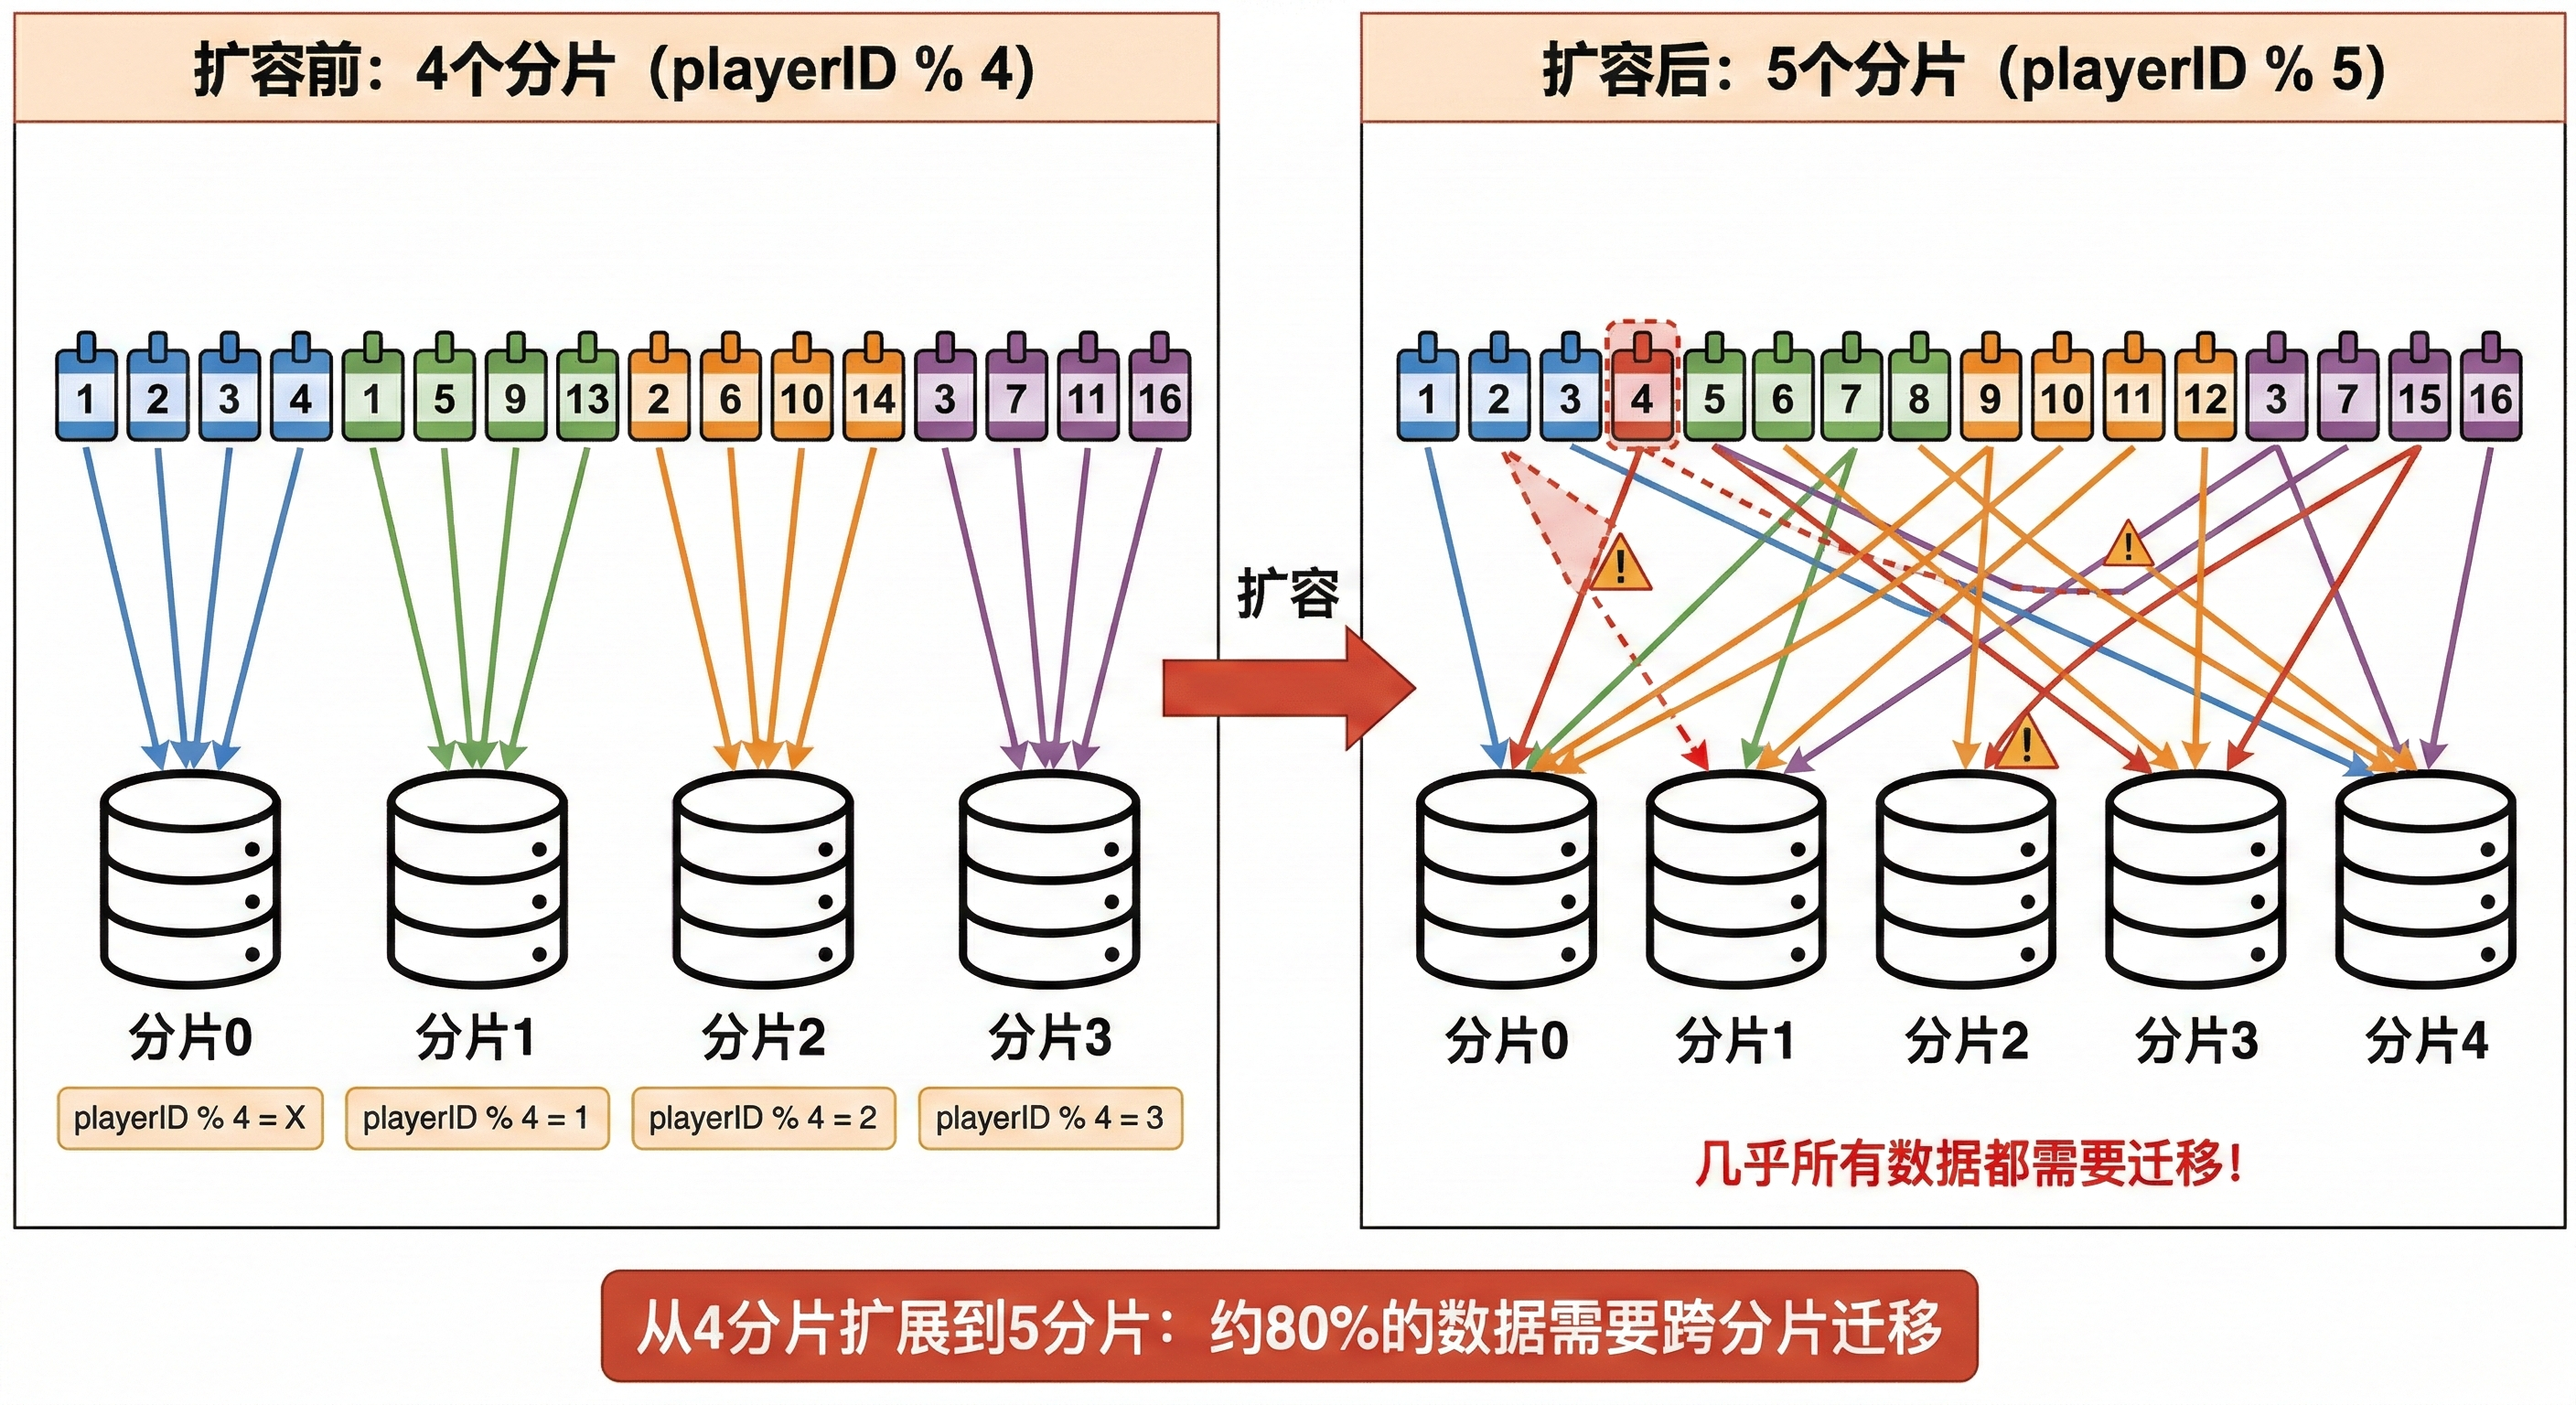
\includegraphics[width=1\linewidth]{figures/sec4/4-6-1.png}
    \caption{哈希分片扩容的数据迁移代价：从4个分片扩展到5个分片时，取模基数改变导致绝大多数玩家的分片归属发生变化，引发大规模数据迁移}
    \label{fig:consistent_hashing}
\end{figure}

但哈希分片也有自己的代价——扩容困难。当我们需要增加数据库实例数量时，比如从 4 个分片扩展到 5 个，取模的基数从 4 变成了 5，这意味着几乎所有玩家的哈希结果都会发生变化。原本 \texttt{playerID \% 4 = 1} 的玩家，现在 \texttt{playerID \% 5} 的结果可能变成 2 或 3 或其他值。这就要求我们重新计算每个玩家应该在哪个分片，并将大量数据从原分片迁移到新分片。对于一个拥有数百万玩家的游戏来说，这种大规模的数据迁移不仅耗时巨大，还可能在迁移过程中影响系统的可用性。

为了缓解扩容时的数据迁移问题，第三种方案是一致性哈希（Consistent Hashing）。一致性哈希的核心思想是将数据库实例和玩家 ID 都映射到一个虚拟的哈希环上——可以想象成一个钟表的表盘，刻度从 0 到 $2^{32}-1$（或其他上限值）。首先，我们将每个数据库实例通过哈希函数映射到环上的某个位置；然后，对于每个玩家 ID，也通过同样的哈希函数映射到环上的某个位置，再在环上顺时针寻找最近的数据库实例节点，这个节点就是该玩家数据存放的位置。

\begin{figure}[htbp]
    \centering
    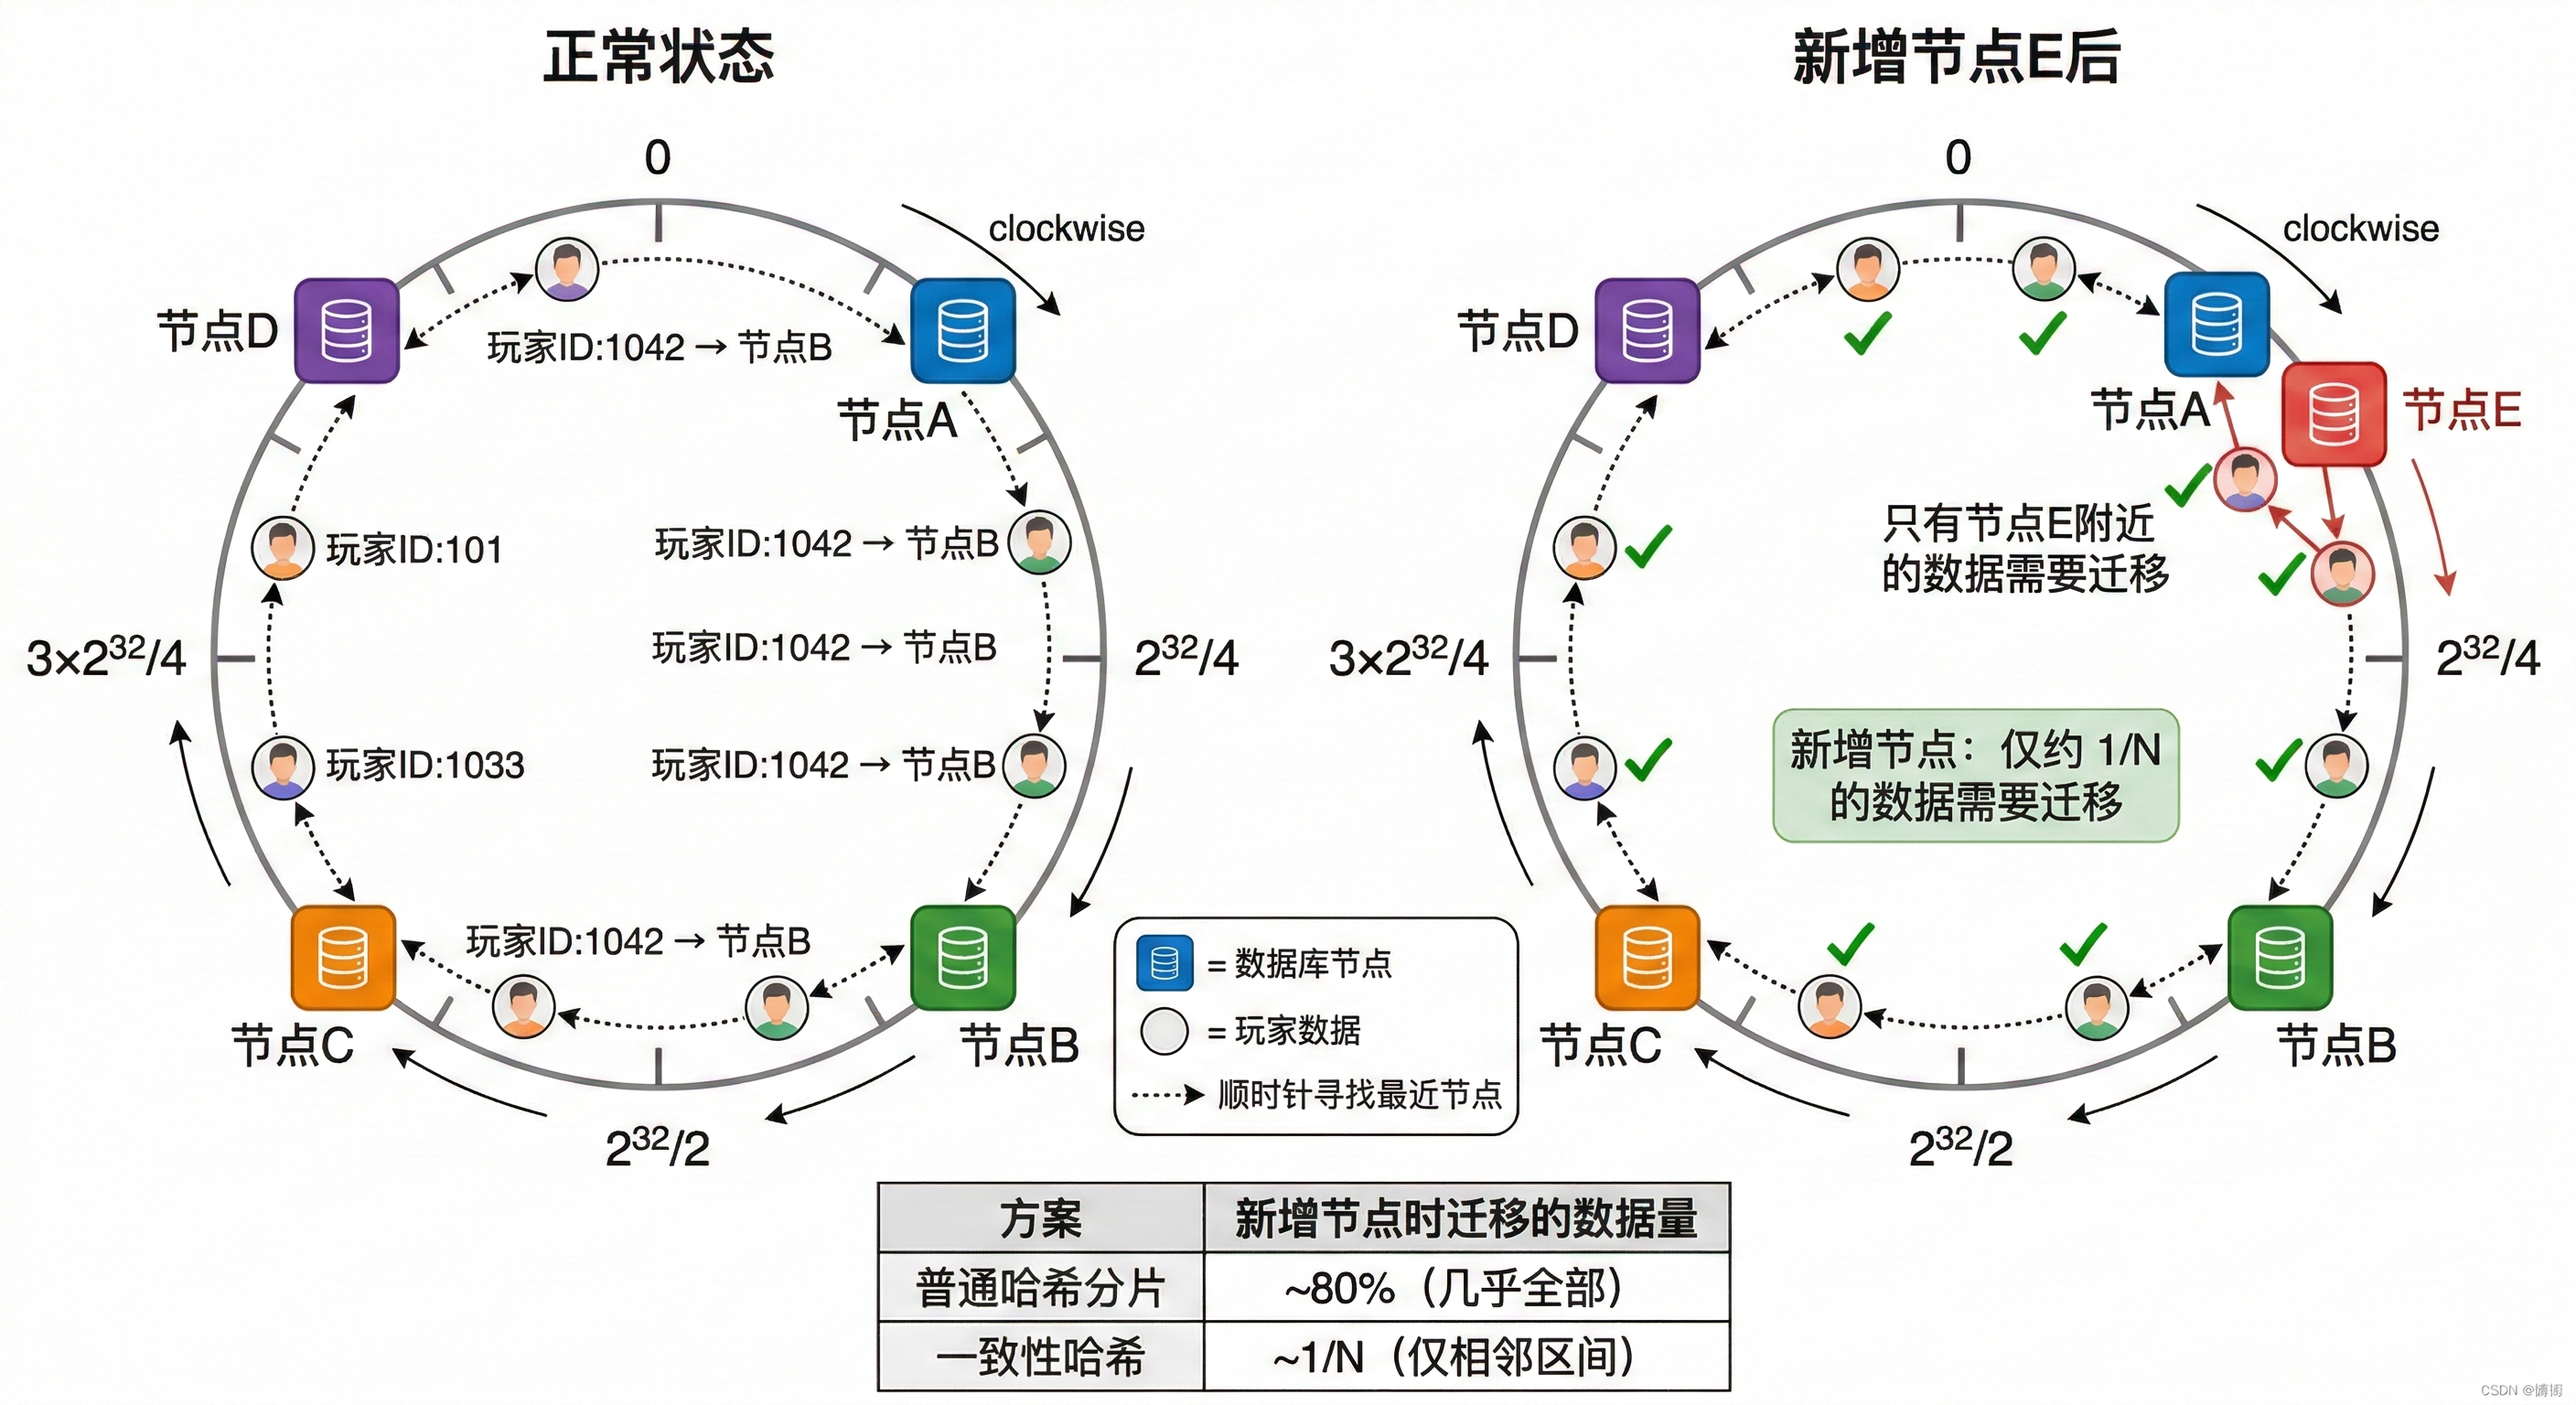
\includegraphics[width=1\linewidth]{figures/sec4/4-6.png}
    \caption{一致性哈希环示意：数据库节点与玩家ID均映射到哈希环上，玩家数据存储在顺时针方向最近的节点；新增节点时，只有该节点附近区间的数据需要迁移，大幅降低扩容成本}
    \label{fig:consistent_hashing}
\end{figure}

\subsubsection{一致性哈希的算法描述}

一致性哈希算法由三个核心操作组成：构建哈希环、路由查询和节点变更。哈希环本质上是一个有序的键值映射结构，其中键是哈希值（整数），值是对应的数据库节点标识。初始化时，对每个数据库节点的标识（如节点名称或 IP 地址）应用哈希函数，将得到的哈希值作为该节点在环上的位置。为了保证负载均衡，通常还会引入虚拟节点：每个物理节点对应环上的多个位置，每个位置通过对节点标识加上不同的后缀再次哈希得到。哈希环使用有序列表维护所有虚拟节点的位置，这是为了在查询时能够使用二分查找，将路由的时间复杂度控制在 $O(\log n)$，其中 $n$ 是虚拟节点的总数。虚拟节点的键由"节点名\#副本编号"拼接后哈希得到，确保同一物理节点的多个虚拟节点在环上的分布尽量分散，从而让不同物理节点负责的数据区间趋于均匀。

\begin{tcolorbox}[title=算法一：构建一致性哈希环]
\begin{lstlisting}[style=codeblock, language=go]
type HashRing struct {
    ring     map[uint32]string
    sorted   []uint32
    replicas int
}

func BuildRing(nodes []string, replicas int) *HashRing {
    r := &HashRing{
        ring:     make(map[uint32]string),
        replicas: replicas,
    }
    for _, node := range nodes {
        AddNode(r, node)
    }
    return r
}

func AddNode(r *HashRing, node string) {
    for i := 0; i < r.replicas; i++ {
        key := hash(fmt.Sprintf("%s#%d", node, i))
        r.ring[key] = node
        r.sorted = append(r.sorted, key)
    }
    sort.Slice(r.sorted, func(i, j int) bool {
        return r.sorted[i] < r.sorted[j]
    })
}
\end{lstlisting}
\end{tcolorbox}

给定一个玩家 ID，查询其应存放的数据库节点时，算法首先对玩家 ID 求哈希，得到其在环上的位置，然后在有序的虚拟节点列表中找到第一个大于等于该位置的节点，即为顺时针方向最近的节点。若玩家的哈希值大于环上所有节点的位置（即已经超过了最大刻度），则顺时针绕回环的起点，取第一个节点。路由查询的正确性依赖于"顺时针最近"的语义——对于任意玩家 ID，其归属节点唯一确定，不存在歧义。这也保证了在节点集合不变的情况下，同一个玩家 ID 每次查询都会路由到同一个节点，满足缓存和分片场景下的稳定性要求。

\begin{tcolorbox}[title=算法二：路由查询]
\begin{lstlisting}[style=codeblock, language=go]
func Lookup(r *HashRing, playerID string) string {
    if len(r.ring) == 0 {
        return ""
    }
    h := hash(playerID)
    idx := sort.Search(len(r.sorted), func(i int) bool {
        return r.sorted[i] >= h
    })
    if idx == len(r.sorted) {
        idx = 0
    }
    return r.ring[r.sorted[idx]]
}
\end{lstlisting}
\end{tcolorbox}

一致性哈希的核心优势体现在节点变更时的迁移范围。当新增一个物理节点时，该节点的若干虚拟节点被插入哈希环。对于每一个新插入的虚拟节点 $v_{new}$，设其在环上的位置为 $p_{new}$，其顺时针方向的下一个节点为 $v_{next}$，位置为 $p_{next}$。那么，只有原本落在区间 $(p_{prev},\, p_{new}]$ 内的玩家数据需要从 $v_{next}$ 迁移到 $v_{new}$，其中 $p_{prev}$ 是 $v_{new}$ 逆时针方向的前一个节点位置，环上其余区间的数据归属完全不受影响。整体迁移量约占全部数据的 $\frac{1}{N+1}$，其中 $N$ 为原有物理节点数。当 $N = 4$ 时，新增第 5 个节点仅需迁移约 $20\%$ 的数据，而普通哈希分片在同等情况下需要迁移约 $80\%$，体现出一致性哈希在水平扩展场景下的显著优势。

\begin{tcolorbox}[title=算法三：新增节点时计算需要迁移的数据范围]
\begin{lstlisting}[style=codeblock, language=go]
type MigrateRange struct {
    From     string
    To       string
    StartKey uint32
    EndKey   uint32
}

func MigrateRanges(r *HashRing, newNode string) []MigrateRange {
    var ranges []MigrateRange
    for i := 0; i < r.replicas; i++ {
        newKey := hash(fmt.Sprintf("%s#%d", newNode, i))
        idx := sort.SearchUints(r.sorted, newKey)
        var prevKey uint32
        if idx == 0 {
            prevKey = r.sorted[len(r.sorted)-1]
        } else {
            prevKey = r.sorted[idx-1]
        }
        srcNode := r.ring[r.sorted[idx%len(r.sorted)]]
        ranges = append(ranges, MigrateRange{
            From:     srcNode,
            To:       newNode,
            StartKey: prevKey,
            EndKey:   newKey,
        })
    }
    return ranges
}
\end{lstlisting}
\end{tcolorbox}

从算法三可以清楚地看到，需要迁移的数据区间数量等于虚拟节点数 \texttt{replicas}，而每个区间的大小约为 $\frac{1}{N+1}$ 的环空间。这种局部迁移的特性，使得系统能够更加平滑地进行水平扩展，减少了扩容对线上服务的影响。

一致性哈希的优势在于扩容时的迁移成本大大降低。当我们新增一个数据库实例时，只有环上部分位置的数据需要迁移——具体来说，只有新实例与其顺时针方向下一个实例之间的那一段数据需要重新分配，其他数据则保持不变。假设原本有 4 个分片均匀分布在环上，每个分片负责 25\% 的数据；当我们新增第 5 个分片时，只有约 20\% 的数据需要迁移，其余 80\% 的数据不受影响。

在实际应用中，为了进一步提升负载均衡的效果，通常会引入虚拟节点的概念。每个物理数据库实例在哈希环上不是只占据一个位置，而是对应多个虚拟节点（比如 150 个），这些虚拟节点均匀分布在环上。这样做的好处是即使物理节点数量较少，也能通过虚拟节点实现更均匀的数据分布，避免因哈希函数的随机性导致某些物理节点负载过高。虚拟节点数 \texttt{replicas} 的选择需要在负载均衡精度和内存开销之间取得平衡：虚拟节点数越多，各物理节点在环上的分布越均匀，负载偏差越小，但同时哈希环占用的内存也线性增长，查询时的二分查找开销也略有上升。在实际工程中，每个物理节点配置 100 到 200 个虚拟节点是常见的经验值，此时各节点的负载标准差通常可以控制在 5\% 以内，足以满足生产环境的均衡要求。对于我们的游戏服务器场景，若有 4 个数据库分片，配置 150 个虚拟节点意味着哈希环上共有 600 个条目，内存开销极小，但负载分布已经足够均匀，是工程性价比较高的选择。

\subsubsection{分片路由的实现}

理解了分片策略之后，接下来需要解决的问题是：应用层如何知道某个玩家的数据在哪个分片上？这就需要实现一个分片路由层。分片路由层维护着分片规则和分片实例信息，负责将应用层的数据库请求转发到正确的分片上。

最直接的实现方式是在应用层代码中嵌入分片路由逻辑。应用服务器启动时，从配置文件或配置中心读取分片规则（比如使用哈希分片，共 4 个分片）和各分片的数据库连接信息（IP 地址、端口、账号密码等），构建一个分片路由表。当需要查询某个玩家的数据时，应用层先根据玩家 ID 和分片规则计算出目标分片编号，再从路由表中获取对应的数据库连接，最后向该数据库发起查询。

\begin{tcolorbox}[title=应用层分片路由的实现示例]
\begin{lstlisting}[
    language=go,
    basicstyle=\ttfamily\footnotesize,
    aboveskip=0pt, belowskip=0pt,
    lineskip=-1pt,
    commentstyle=\color{gray},
    keywordstyle=\color{blue}\bfseries,
    breaklines=true
]
// 分片路由器
type ShardRouter struct {
    numShards int
    dbConnections []*sql.DB  // 各分片的数据库连接
}

// 根据玩家ID获取目标分片的数据库连接
func (r *ShardRouter) getDBConnection(playerID int) *sql.DB {
    shardID := playerID % r.numShards
    return r.dbConnections[shardID]
}

// 查询玩家数据
func (r *ShardRouter) queryPlayer(playerID int) (*Player, error) {
    // 1. 计算目标分片
    db := r.getDBConnection(playerID)
    
    // 2. 向目标分片发起查询
    var player Player
    err := db.QueryRow(
        "SELECT id, name, power FROM players WHERE id = ?",
        playerID,
    ).Scan(&player.ID, &player.Name, &player.Power)
    
    return &player, err
}
\end{lstlisting}
\end{tcolorbox}

这种应用层路由的优点是实现简单、性能开销低——路由计算只是一个简单的取模操作，几乎不消耗时间。但缺点也很明显：分片逻辑与业务代码耦合在一起，如果需要调整分片策略（比如从哈希分片改为一致性哈希）或增加分片数量，可能需要修改应用层代码并重新部署。

另一种实现方式是引入数据库代理中间件（Database Proxy）。中间件作为独立的服务部署在应用服务器和数据库之间，应用层不再直接连接各个分片，而是统一连接到中间件。中间件负责接收应用层的 SQL 请求，解析 SQL 语句，提取分片键（如 WHERE 子句中的玩家 ID），计算目标分片，将请求转发到对应的数据库实例，最后将结果返回给应用层。这种方式的优点是业务代码与分片逻辑完全解耦，分片策略的调整不需要修改应用代码；缺点是引入了额外的网络跳转和 SQL 解析开销，可能对性能有一定影响。

\subsubsection{分片后的查询与事务挑战}

数据拆分完成之后，应用层所面对的数据库世界已经发生了根本性的变化。这种变化不仅体现在连接方式和路由逻辑上，更深刻地影响了某些类型查询和事务的实现方式。

首先是跨分片查询的问题。前面提到的分片路由，针对的是"查询单个玩家数据"这种场景——给定一个玩家 ID，我们可以明确地知道数据在哪个分片，直接向该分片发起查询即可。但有些查询并不是针对单个玩家的，而是需要聚合多个分片的数据。最典型的例子是全服排行榜：假设我们需要查询战力值排名前一百的玩家。

在单一数据库时代，这只需要执行一条 SQL 语句：

\begin{tcolorbox}[title=单一数据库中的排行榜查询]
\begin{lstlisting}[
    language=SQL,
    basicstyle=\ttfamily\footnotesize,
    aboveskip=0pt, belowskip=0pt,
    lineskip=-1pt,
    commentstyle=\color{gray},
    keywordstyle=\color{blue}\bfseries,
    breaklines=true
]
SELECT id, name, power 
FROM players 
ORDER BY power DESC 
LIMIT 100;
-- 数据库自动扫描所有玩家，按战力排序，返回前100名
\end{lstlisting}
\end{tcolorbox}

但在数据拆分之后，不同玩家的数据分散在不同的分片中。应用层需要采用"分散查询、集中汇总"的策略：首先向所有分片分别发起查询，每个分片返回自己负责的那部分玩家中战力值最高的 100 个；然后应用层将这些结果合并到一起（比如分片 0 返回 100 个，分片 1 返回 100 个，分片 2 返回 100 个，分片 3 返回 100 个，总共 400 个），在应用层重新排序，最终截取战力值最高的 100 个作为全服排行榜。

\begin{tcolorbox}[title=分片环境下的排行榜查询]
\begin{lstlisting}[
    language=go,
    basicstyle=\ttfamily\footnotesize,
    aboveskip=0pt, belowskip=0pt,
    lineskip=-1pt,
    commentstyle=\color{gray},
    keywordstyle=\color{blue}\bfseries,
    breaklines=true
]
func (r *ShardRouter) getRanking() ([]Player, error) {
    var allResults []Player
    
    // 1. 向所有分片并发发起查询
    for i := 0; i < r.numShards; i++ {
        var shardResults []Player
        rows, _ := r.dbConnections[i].Query(
            "SELECT id, name, power FROM players ORDER BY power DESC LIMIT 100",
        )
        // 读取该分片的Top100到shardResults...
        allResults = append(allResults, shardResults...)
    }
    
    // 2. 在应用层合并并重新排序
    sort.Slice(allResults, func(i, j int) bool {
        return allResults[i].Power > allResults[j].Power
    })
    
    // 3. 截取最终的Top100
    if len(allResults) > 100 {
        allResults = allResults[:100]
    }
    
    return allResults, nil
}
\end{lstlisting}
\end{tcolorbox}

这种跨分片查询的效率明显低于单库查询。首先，需要向多个分片发起查询，网络开销成倍增加；其次，每个分片都要执行完整的排序操作，计算资源消耗是单库的数倍；最后，应用层还需要对合并后的结果进行二次排序，增加了应用服务器的 CPU 负担。因此，在设计分片策略时，应尽量避免频繁的跨分片查询。对于排行榜这类必须进行全局聚合的数据，更好的做法是采用异步汇总：通过后台定时任务，定期从各个分片拉取数据并汇总到一个专门的"排行榜缓存"中（比如 Redis），玩家查询排行榜时直接读取缓存，而不是实时跨分片查询。

更棘手的是跨分片事务问题。在我们的对战游戏中，假设玩家 A（ID 为 1001，存储在分片 1）与玩家 B（ID 为 2002，存储在分片 2）进行了一场战斗。战斗结束后，需要同时更新两位玩家的战绩：

\begin{enumerate}
\item 在分片 1 中更新玩家 A 的胜场数：\texttt{UPDATE players SET wins = wins + 1 WHERE id = 1001}
\item 在分片 2 中更新玩家 B 的负场数：\texttt{UPDATE players SET losses = losses + 1 WHERE id = 2002}
\end{enumerate}

在单一数据库中，这两个操作可以放在同一个事务中，数据库保证要么全部成功
（玩家 A 的胜场加一，玩家 B 的败场加一），要么全部失败（都回滚，谁的战绩都不变）。
但在拆分后的世界里，这两个操作分别发生在两个独立的数据库实例上。
如果简单地依次执行，就可能出现"部分成功"的情况：
第一个操作成功了（A 的胜场已经加一），第二个操作却因为网络故障失败了（B 的败场没有更新），
数据库里就留下了一场只有赢家、没有输家的战斗记录——这正是分布式环境下事务一致性问题的典型表现。

要解决跨分片事务问题，需要引入分布式事务协议，最经典的是两阶段提交协议
（Two-Phase Commit，2PC）。其完整流程如图~\ref{fig:2pc} 所示。
第一阶段称为准备阶段（Prepare Phase）：由一个协调者（Coordinator）同时向所有参与事务的分片
发出"准备提交"请求（图中步骤①）。各分片收到请求后，在本地执行操作并将结果写入事务日志，
但不立即提交，而是对相关数据行加锁以防止其他事务并发修改，然后向协调者回复"就绪"
（Vote: Ready）或"失败"（Vote: Abort）（图中步骤②）。
这把锁不会在准备阶段结束——它必须一直持续到协调者发出第二阶段的最终指令为止，
图中红色括注的区间正是行锁被持有的全程，这也是 2PC 拉长锁持有时间、降低并发度的根本原因。

第二阶段称为提交阶段（Commit Phase）：协调者收集完所有分片的投票后进行裁决（图中步骤③）。
若所有分片均回复"就绪"，协调者向所有分片广播"正式提交"指令，
各分片将准备好的操作真正落库并释放行锁（图中成功路径步骤④）；
若任意一个分片回复"失败"，或协调者在超时时间内未收到全部响应，
则广播"回滚"指令，各分片撤销准备阶段的操作并同样释放锁（图中失败路径步骤④）。
在我们的战斗场景中，这意味着玩家 A 的胜场更新和玩家 B 的败场更新要么同时落库，
要么同时撤销，从协议层面保证了跨分片操作的原子性。

然而 2PC 的代价是显著的，体现在图中三个灰色注记上。
其一，整个流程涉及两轮网络往返——准备阶段一轮，提交阶段一轮——
每轮都需要协调者与全部参与分片完成请求和响应，事务的端到端延迟远高于单分片事务。
其二，准备阶段到提交阶段之间行锁持续持有，其他需要读写同一数据行的事务都要排队等待，
在高并发的游戏场景下这会显著压缩系统的吞吐量上限。
其三，协调者存在单点崩溃风险：若协调者在广播"准备"之后、发出"提交"之前宕机，
各分片将永远停留在"就绪"状态，行锁无法自动释放，后续所有操作都会被阻塞，
必须依靠超时机制或人工介入才能恢复，这在生产环境中是极难排查的故障场景。

\begin{figure}[htbp]
    \centering
    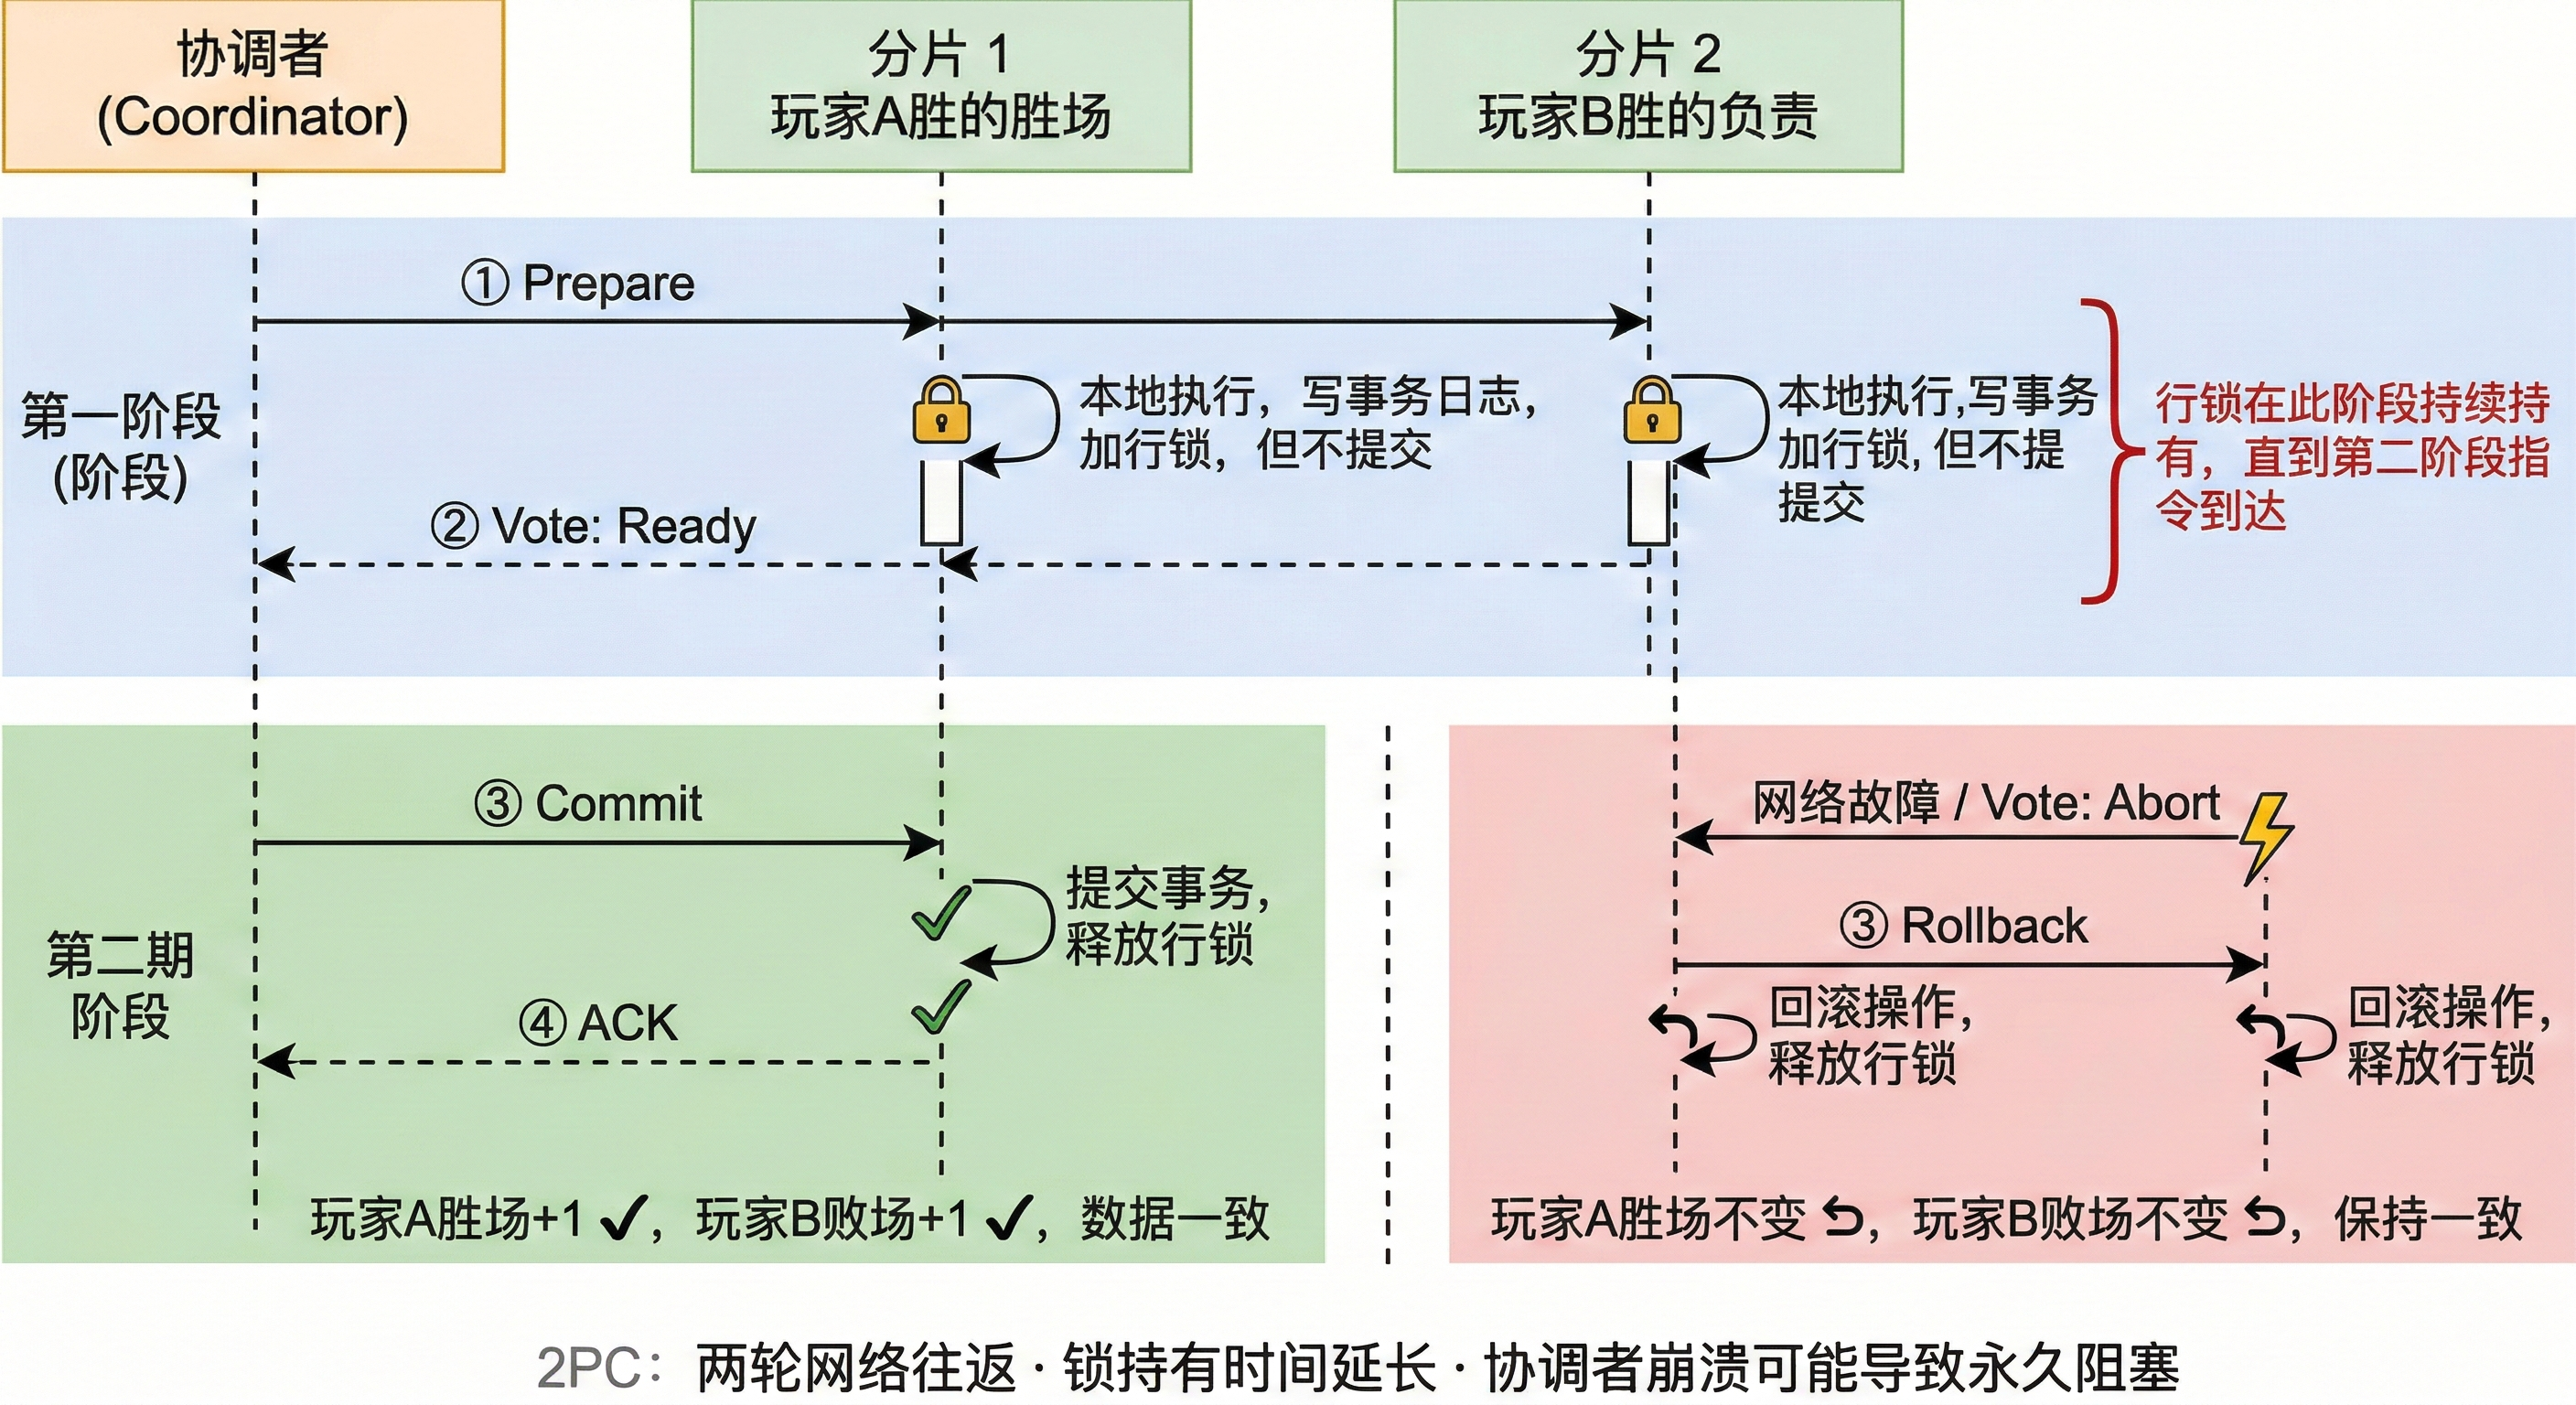
\includegraphics[width=1\linewidth]{figures/sec4/两阶段提交.png}
    \caption{两阶段提交协议（2PC）的时序图：第一阶段协调者收集各分片的投票并持锁等待，
    第二阶段根据投票结果广播提交或回滚指令；红色括注区间为行锁持有期，
    右侧失败路径展示协调者收到 Abort 或超时后触发全局回滚的流程}
    \label{fig:2pc}
\end{figure}

因此，在实际工程中引入 2PC 的代价往往超过其带来的收益。
更实用的做法是从业务设计层面入手，将跨分片操作转化为可以在单分片内完成的操作，
或者接受短暂的数据不一致并通过异步机制保证最终收敛。
这里介绍两种常见的工程策略。

第一种策略是异步消息队列。战斗结束后，战斗服务器不直接向两个分片发起写操作，
而是将战斗结果——包括双方玩家 ID、胜负情况、时间戳——作为一条消息投递到消息队列。
专门的战绩更新服务从队列中消费消息，依次向各分片发起更新；
若某次更新因分片暂时不可用而失败，消息会保留在队列中持续重试，最终一定会被成功处理，
不存在"永久丢失"的风险。这种方案以"最终一致性"替代"强一致性"——
战绩会在数秒内更新完毕，对玩家几乎无感知，系统换来的是更高的可用性和远低于 2PC 的实现复杂度。
需要注意的是，消息队列本身必须具备持久化和至少一次投递的保障，
否则队列自身的故障反而会成为新的数据丢失入口。

第二种策略是重新设计数据模型，从根本上消除跨分片事务存在的前提。
如果战绩是高频写入的核心数据，可以将战绩从玩家分片中完全剥离，
交由一个独立的战绩服务集中管理。这个服务可以使用单一数据库（若数据量可控），
也可以使用专门为追加写入优化的时序数据库，所有对战绩的读写操作都发生在该服务内部，
从结构上不再存在跨分片写入的问题。代价是系统多了一个独立服务和对应的数据库，
运维复杂度略有上升；但换来的是战绩访问路径的简单清晰——
尤其对于玩家查询历史对战记录这类高频只读场景，单服务内的查询比跨分片聚合要高效得多。


\subsubsection{容错机制与备份策略}

数据拆分到多个数据库实例之后，虽然降低了单点故障的全局影响，但每个数据库实例仍然需要有自己的容错机制。最常见的做法是为每个数据库实例部署主从复制架构（Master-Slave Replication）。

在主从架构中，每个分片包含一个主库（Master）和一个或多个从库（Slave）。主库负责处理所有的写操作（INSERT、UPDATE、DELETE），从库通过 binlog（二进制日志）实时同步主库的数据变化，并承担读操作的负载。具体的同步过程是：主库在执行每个写操作时，会将操作记录到 binlog 中；从库会持续监听主库的 binlog，读取新的日志条目，并在本地重放（Replay）这些操作，从而保持与主库的数据一致。

\begin{figure}[htbp]
    \centering
    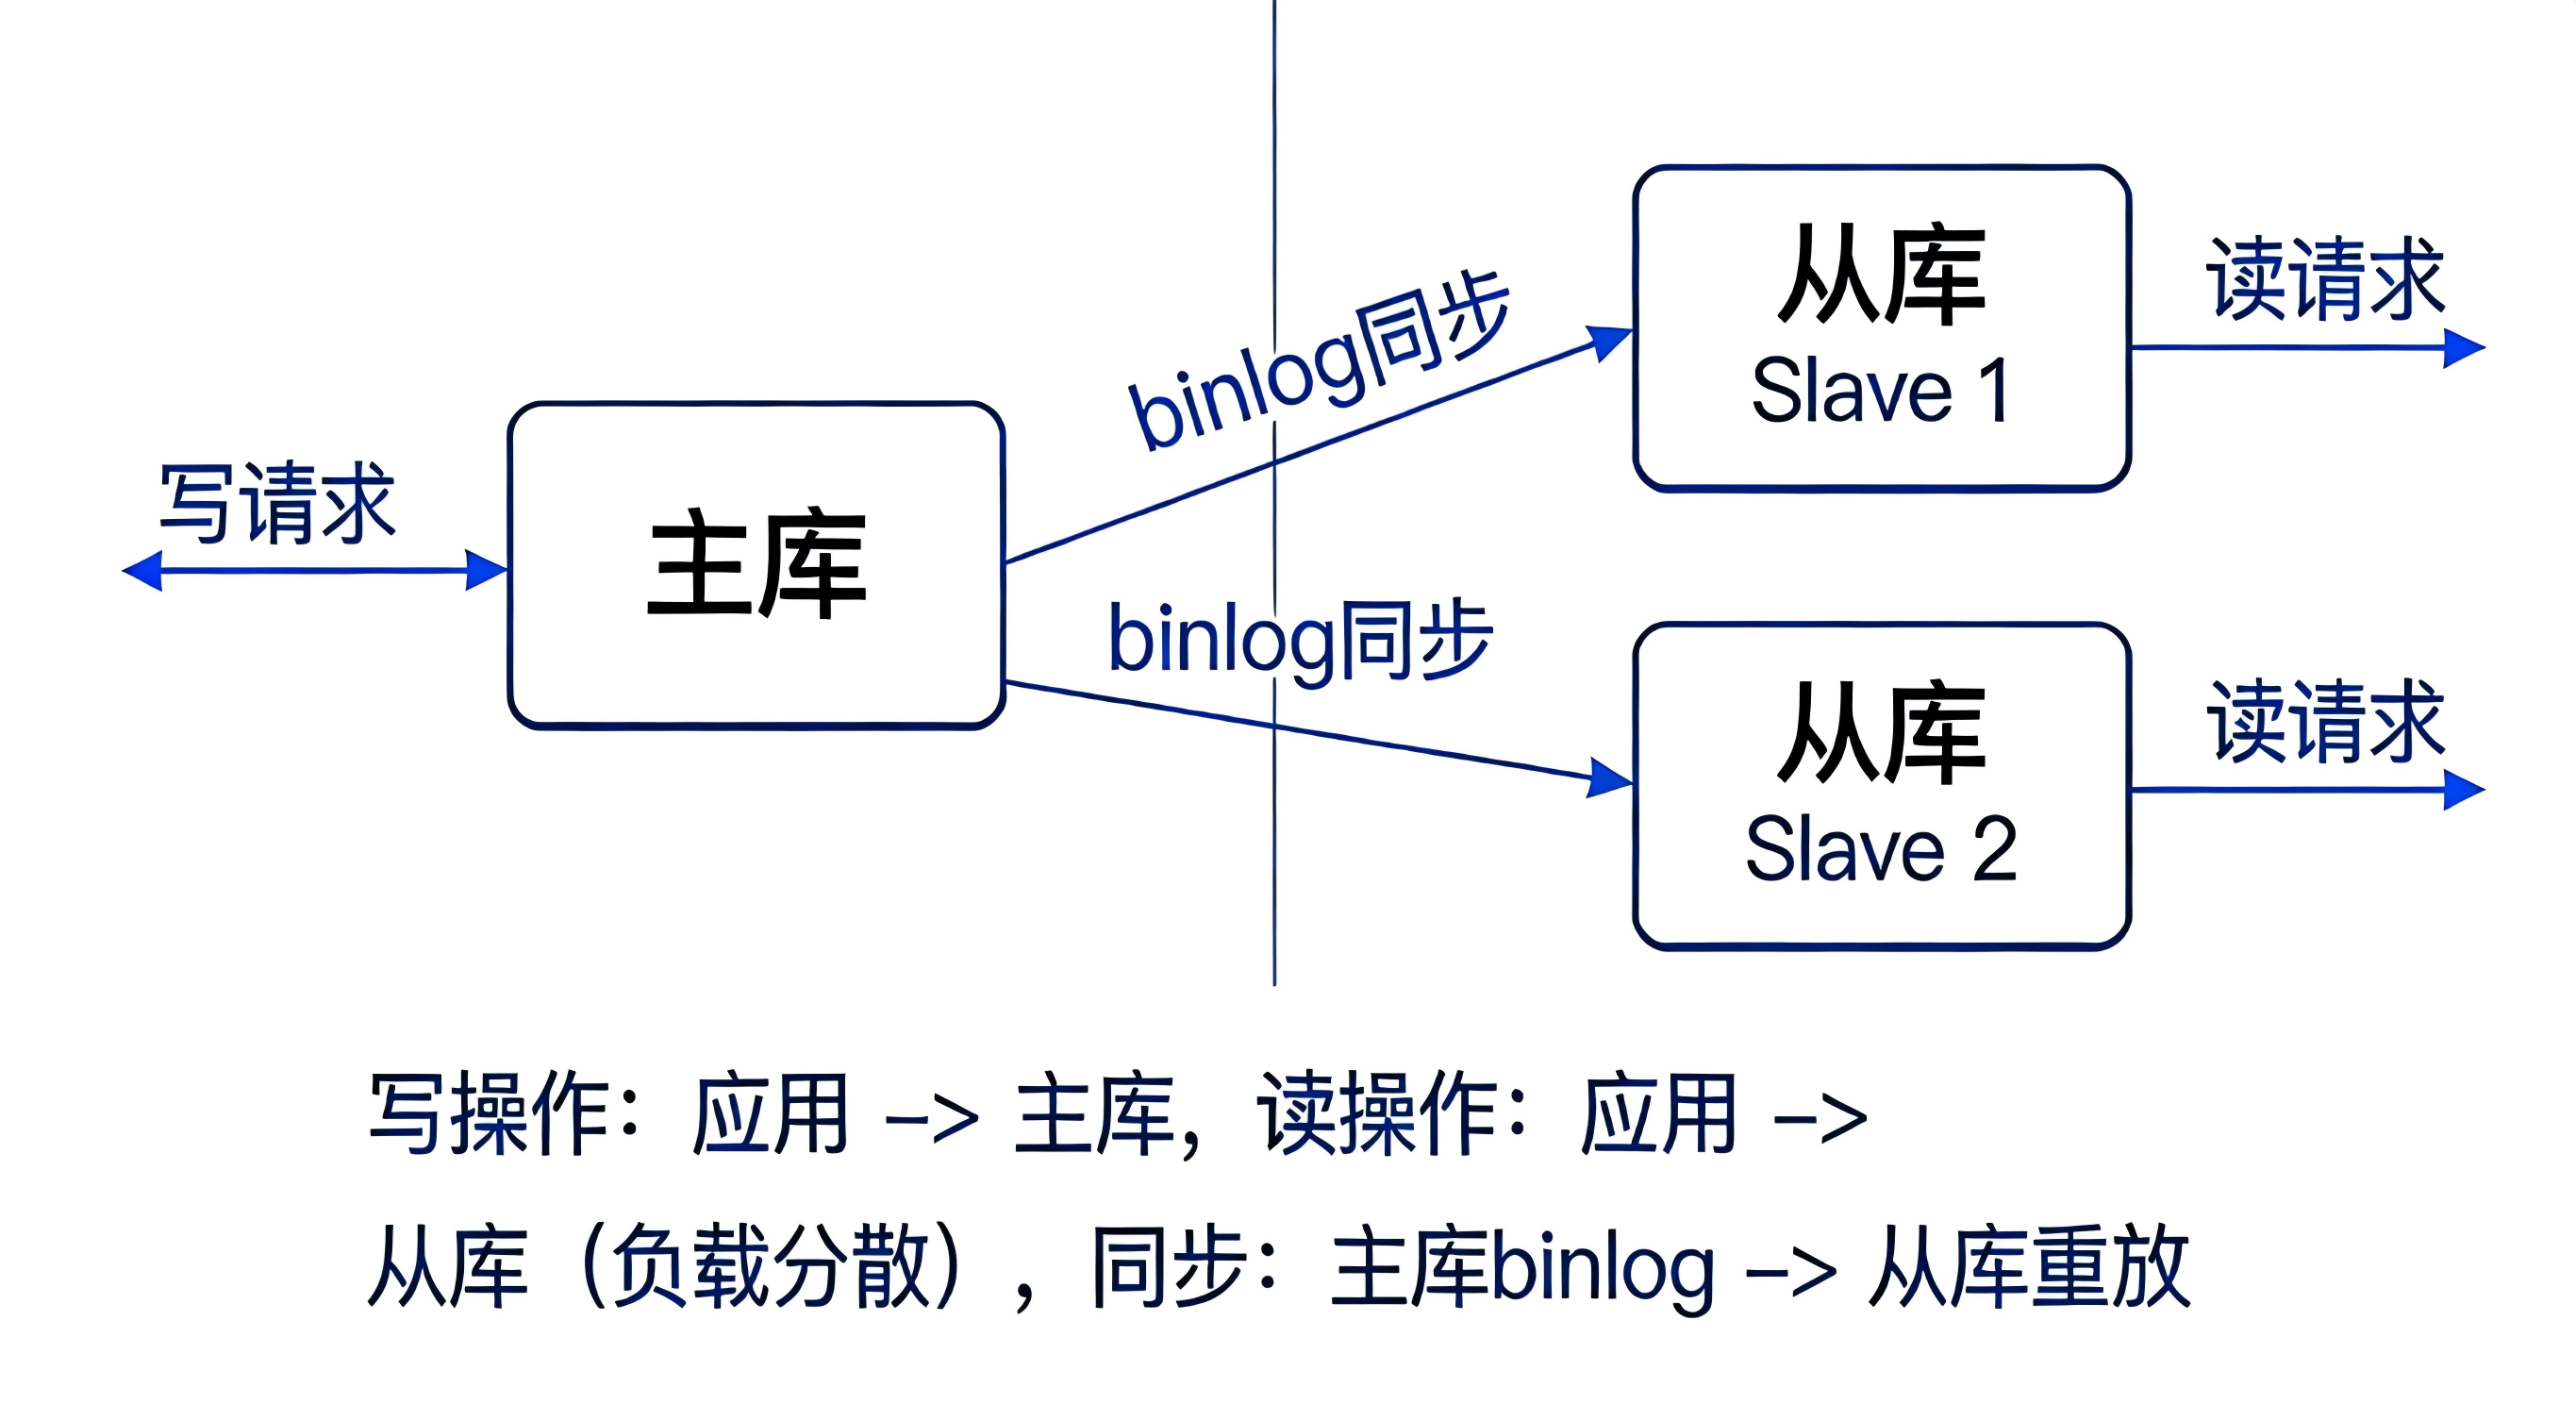
\includegraphics[width=1\linewidth]{figures/sec4/4-3.png}
    % 图片描述：主从复制架构示意图
    % 左侧：一个"主库"矩形框，标注"Master"，接收"写请求"箭头
    % 右侧：两个"从库"矩形框，标注"Slave 1"和"Slave 2"，接收"读请求"箭头
    % 主库向两个从库各有一条箭头，标注"binlog同步"
    % 下方用文字说明：
    %   - 写操作：应用 -> 主库
    %   - 读操作：应用 -> 从库（负载分散）
    %   - 同步：主库binlog -> 从库重放
    % 所有文字使用简体中文
    \caption{数据库主从复制架构}
    \label{fig:master_slave_replication}
\end{figure}

这种主从架构有两个核心好处。第一，提升了读取并发能力。由于大部分游戏场景中读操作远多于写操作（比如玩家登录时读取角色信息、查看背包、查询战绩等），将读请求分散到多个从库上，可以有效降低主库的压力，提升系统的整体查询吞吐量。应用层可以采用简单的轮询策略，将读请求依次分配给不同的从库，或者根据从库的负载情况动态选择。

第二，实现了数据的热备份。当主库出现故障时——比如硬件损坏、进程崩溃、网络中断——可以快速将某个从库提升为新的主库（这个过程称为故障转移，Failover），继续提供服务。具体的故障转移流程通常由自动化工具或数据库代理中间件来完成：首先，通过心跳检测发现主库不可用；然后，从多个从库中选择一个数据最新、延迟最低的作为新主库；接着，通知应用层和其他从库切换连接目标；最后，新主库开始接收写请求，其他从库从新主库同步数据。整个过程通常可以在数十秒内完成，大大缩短了故障恢复时间。

除了主从复制，还需要建立完善的备份策略。主从复制虽然提供了实时的热备份，但它无法防范某些类型的错误——比如误操作删除了大量数据，或者数据被恶意篡改。这种情况下，从库会同步主库的错误操作，热备份无法起到保护作用。因此，我们还需要定期执行冷备份：

全量备份（Full Backup）：定期（比如每天凌晨）对整个数据库做一次完整的快照，导出所有表的数据和结构，存储到独立的备份服务器或云存储服务（如 Amazon S3、阿里云 OSS）中。全量备份的好处是恢复简单——只需要将备份文件导入即可恢复到备份时刻的完整状态；缺点是备份文件较大，占用存储空间多，备份和恢复过程耗时较长。

增量备份（Incremental Backup）：在两次全量备份之间，定期（比如每小时）备份自上次备份以来发生变化的数据。增量备份通常通过备份 binlog 来实现——binlog 记录了所有的数据变更操作，通过重放 binlog 可以将数据库恢复到任意时间点。增量备份的好处是备份文件小、备份速度快；缺点是恢复时需要先恢复最近的全量备份，再依次重放所有增量备份，过程较复杂。

在实际部署中，通常会结合全量备份和增量备份：每天做一次全量备份，每小时做一次增量备份。这样，当需要恢复数据时，可以先恢复最近的全量备份（比如昨天凌晨的），再重放之后的增量备份（昨天凌晨到故障时刻之间的 binlog），将数据恢复到故障发生前的最新状态，数据丢失的时间窗口可以控制在一小时以内。

最后，备份的存在只是保障的第一步，更关键的是要定期进行恢复演练。很多系统在真正需要恢复数据时才发现备份文件损坏、恢复脚本有 bug、或者恢复时间远超预期。因此，建议每月至少进行一次备份恢复演练：在测试环境中，使用真实的备份文件模拟完整的恢复流程，记录恢复所需的时间，发现并修复流程中的问题。通过这些容错机制——主从复制、定期备份、恢复演练——即使某个分片出现故障，也能在最短时间内恢复服务，将对玩家的影响降到最低。



\subsubsection{缓存层的分布式演进：从单机Redis到集群}

% 前面几节讨论了PostgreSQL数据库的分片策略，但不要忘记，在第三章中我们建立的分层存储架构还包含Redis缓存层。当数据库从单实例拆分为多个分片时，Redis同样面临容量和可用性的挑战：单机Redis的内存上限通常在几十GB到上百GB之间，当热数据总量超过这个上限时，单个Redis实例将无法容纳所有在线玩家的实时状态；同时，单机Redis也存在单点故障风险——一旦宕机，所有依赖缓存的热数据访问都会直接穿透到数据库，瞬间压垮后端。

% 解决思路与数据库分片类似：将数据分散到多个Redis节点上。Redis Cluster是官方提供的分布式方案，它将整个键空间划分为16384个哈希槽（Hash Slot），每个节点负责一部分槽位。当应用写入一个键时，Redis客户端通过CRC16哈希算法计算该键应落入哪个槽位，再路由到对应的节点。这种机制与第三章中单机Redis的使用方式在应用层几乎透明——开发者仍然使用相同的SET、GET、ZADD等命令，只是底层的数据分布由集群自动管理。

% 需要注意的是，Redis分片与数据库分片的分片键通常保持一致。如果数据库按玩家ID哈希分片，Redis中以玩家ID为前缀的键（如\texttt{player:1001:pos}、\texttt{player:1001:online}）也应当路由到对应的Redis节点，这样同一个玩家的热数据和冷数据在物理上保持亲和性，避免跨节点访问。对于排行榜这类全局聚合数据，则可以使用独立的Redis实例集中存储，由后台任务定期从各分片汇总更新。

在前文中，我们已经用玩家 ID 作为分片键，将冷数据拆分到多个 PostgreSQL 实例上；从本质上讲，Redis 缓存层面对的是同一类问题：单机内存容量和单点故障风险。当在线玩家规模从几千增长到几十万时，单个 Redis 实例的内存不足以容纳所有玩家的在线状态、实时位置、排行榜片段等热数据，一旦出现故障，所有访问都会瞬间穿透到后端数据库，形成“雪崩效应”。

因此，Redis 层的演进思路与数据库分片是一致的：同样以玩家 ID 作为分片键，将键空间拆分到多个 Redis 节点上，实现容量和吞吐的水平扩展，并通过多节点降低单点故障风险。不同之处在于实现机制：数据库分片可以使用范围分片、哈希分片或一致性哈希，而 Redis 官方的 Redis Cluster 则将整个键空间划分为 16384 个哈希槽（Hash Slot），每个槽位对应一个范围编号，由不同节点负责一部分槽位。

具体来说，当我们在应用中写入一个键时，Redis 客户端会对键名执行 CRC16 哈希运算，再对 16384 取模，得到一个槽位编号；集群根据槽位所属范围，将请求路由到对应节点上。形式上，这与“玩家 ID 经过哈希后落在哈希环上，再映射到某个分片节点”是同一套思路，只是 PostgreSQL 分片由我们自己定义哈希规则，而 Redis Cluster 固定使用“槽位”的抽象。

在具体设计时，有一个需要与数据库分片刻意对齐的点：分片键的一致性。如果数据库是按玩家 ID 进行哈希分片，那么 Redis 中与该玩家相关的缓存键（例如 \texttt{player:1001:pos}、\texttt{player:1001:online}、\texttt{player:1001:inventory}）也应当围绕玩家 ID 组织，并路由到与该玩家冷数据同一个逻辑分片上。对于 Redis Cluster，可以利用哈希标签（Hash Tag）保证相关键落在同一个槽位，例如使用 \texttt{{player:1001}:pos}、\texttt{{player:1001}:online} 的形式，使大括号中的部分作为共同哈希片段，从而将同一玩家的多种状态键聚集在同一节点上，减少跨节点访问和多键操作受限的问题。

% 需要注意的是，Redis 的分片与复制是两条正交的维度：分片解决的是“如何把不同玩家的数据分布到多台节点上”，复制（主从/主备）解决的是“同一份数据如何在多台节点之间做高可用冗余”。在一个成熟的部署中，通常会将前文的思路整体套用到缓存层：每个 Redis 分片节点后面再挂一到多个副本节点，既通过分片实现容量与性能的水平扩展，又通过复制实现故障时的快速切换，避免缓存层成为新的单点短板。

\subsection{负载均衡：合理分配玩家流量}

当数据库和缓存层都完成分布式拆分之后，游戏系统已经具备了在多台机器上存储和管理
玩家数据的能力。但仅有数据层的拆分还不够，计算层——也就是运行游戏逻辑、
处理玩家操作的游戏服务器——同样需要进行扩展和分配。
可以想象这样一个场景：我们把玩家数据分片存储到了四台数据库服务器上，
每台数据库都能稳定地承载 25 万玩家的数据，从存储容量的角度看似乎万事大吉。
但当这 100 万玩家真正上线游戏时，他们需要连接的不是数据库，而是游戏服务器——
游戏服务器负责处理玩家的登录请求、匹配对手、模拟战斗、结算奖励，
这些都是实时的、计算密集的任务。如果我们只部署了一台游戏服务器，
那么即使数据库已经完成了分片，这台游戏服务器仍然会成为新的瓶颈：
它的 CPU 要处理所有玩家的战斗逻辑，它的网络要承载所有玩家的消息收发，
它的内存要维护所有在线玩家的会话状态。

在理解这一问题时，有一个容易产生的误解需要先澄清：游戏服务器与数据库分片之间，
并不存在一一对应的绑定关系。下图展示了这一点。
数据库分片解决的是\textbf{存储层}的问题——将玩家的冷数据按分片键切割，
分散存放到多个独立的数据库实例上，每个分片负责一个哈希区间内的玩家数据。
游戏服务器解决的是\textbf{计算层}的问题——将玩家的实时连接和计算请求分散到多台服务器上，
每台服务器负责维护一部分在线玩家的会话和战斗逻辑。
这两个维度是相互独立的：任意一台游戏服务器在需要读写某个玩家的数据时，
都通过分片路由层计算出目标分片编号，再向对应的数据库实例发起请求——
是"多对多"的访问关系，而不是固定的"服务器 1 专属对应分片 1"的绑定关系。
这种解耦带来了极大的灵活性：当在线玩家数量激增、计算层成为瓶颈时，
我们可以单独增加游戏服务器的数量而无需触动数据库配置；
当玩家数据总量增长、存储层遇到容量上限时，
可以单独为数据库增加新的分片而不必同步扩容游戏服务器。
两个维度按照各自的压力独立伸缩，这正是分层架构的核心价值所在。

\begin{figure}[htbp]
    \centering
    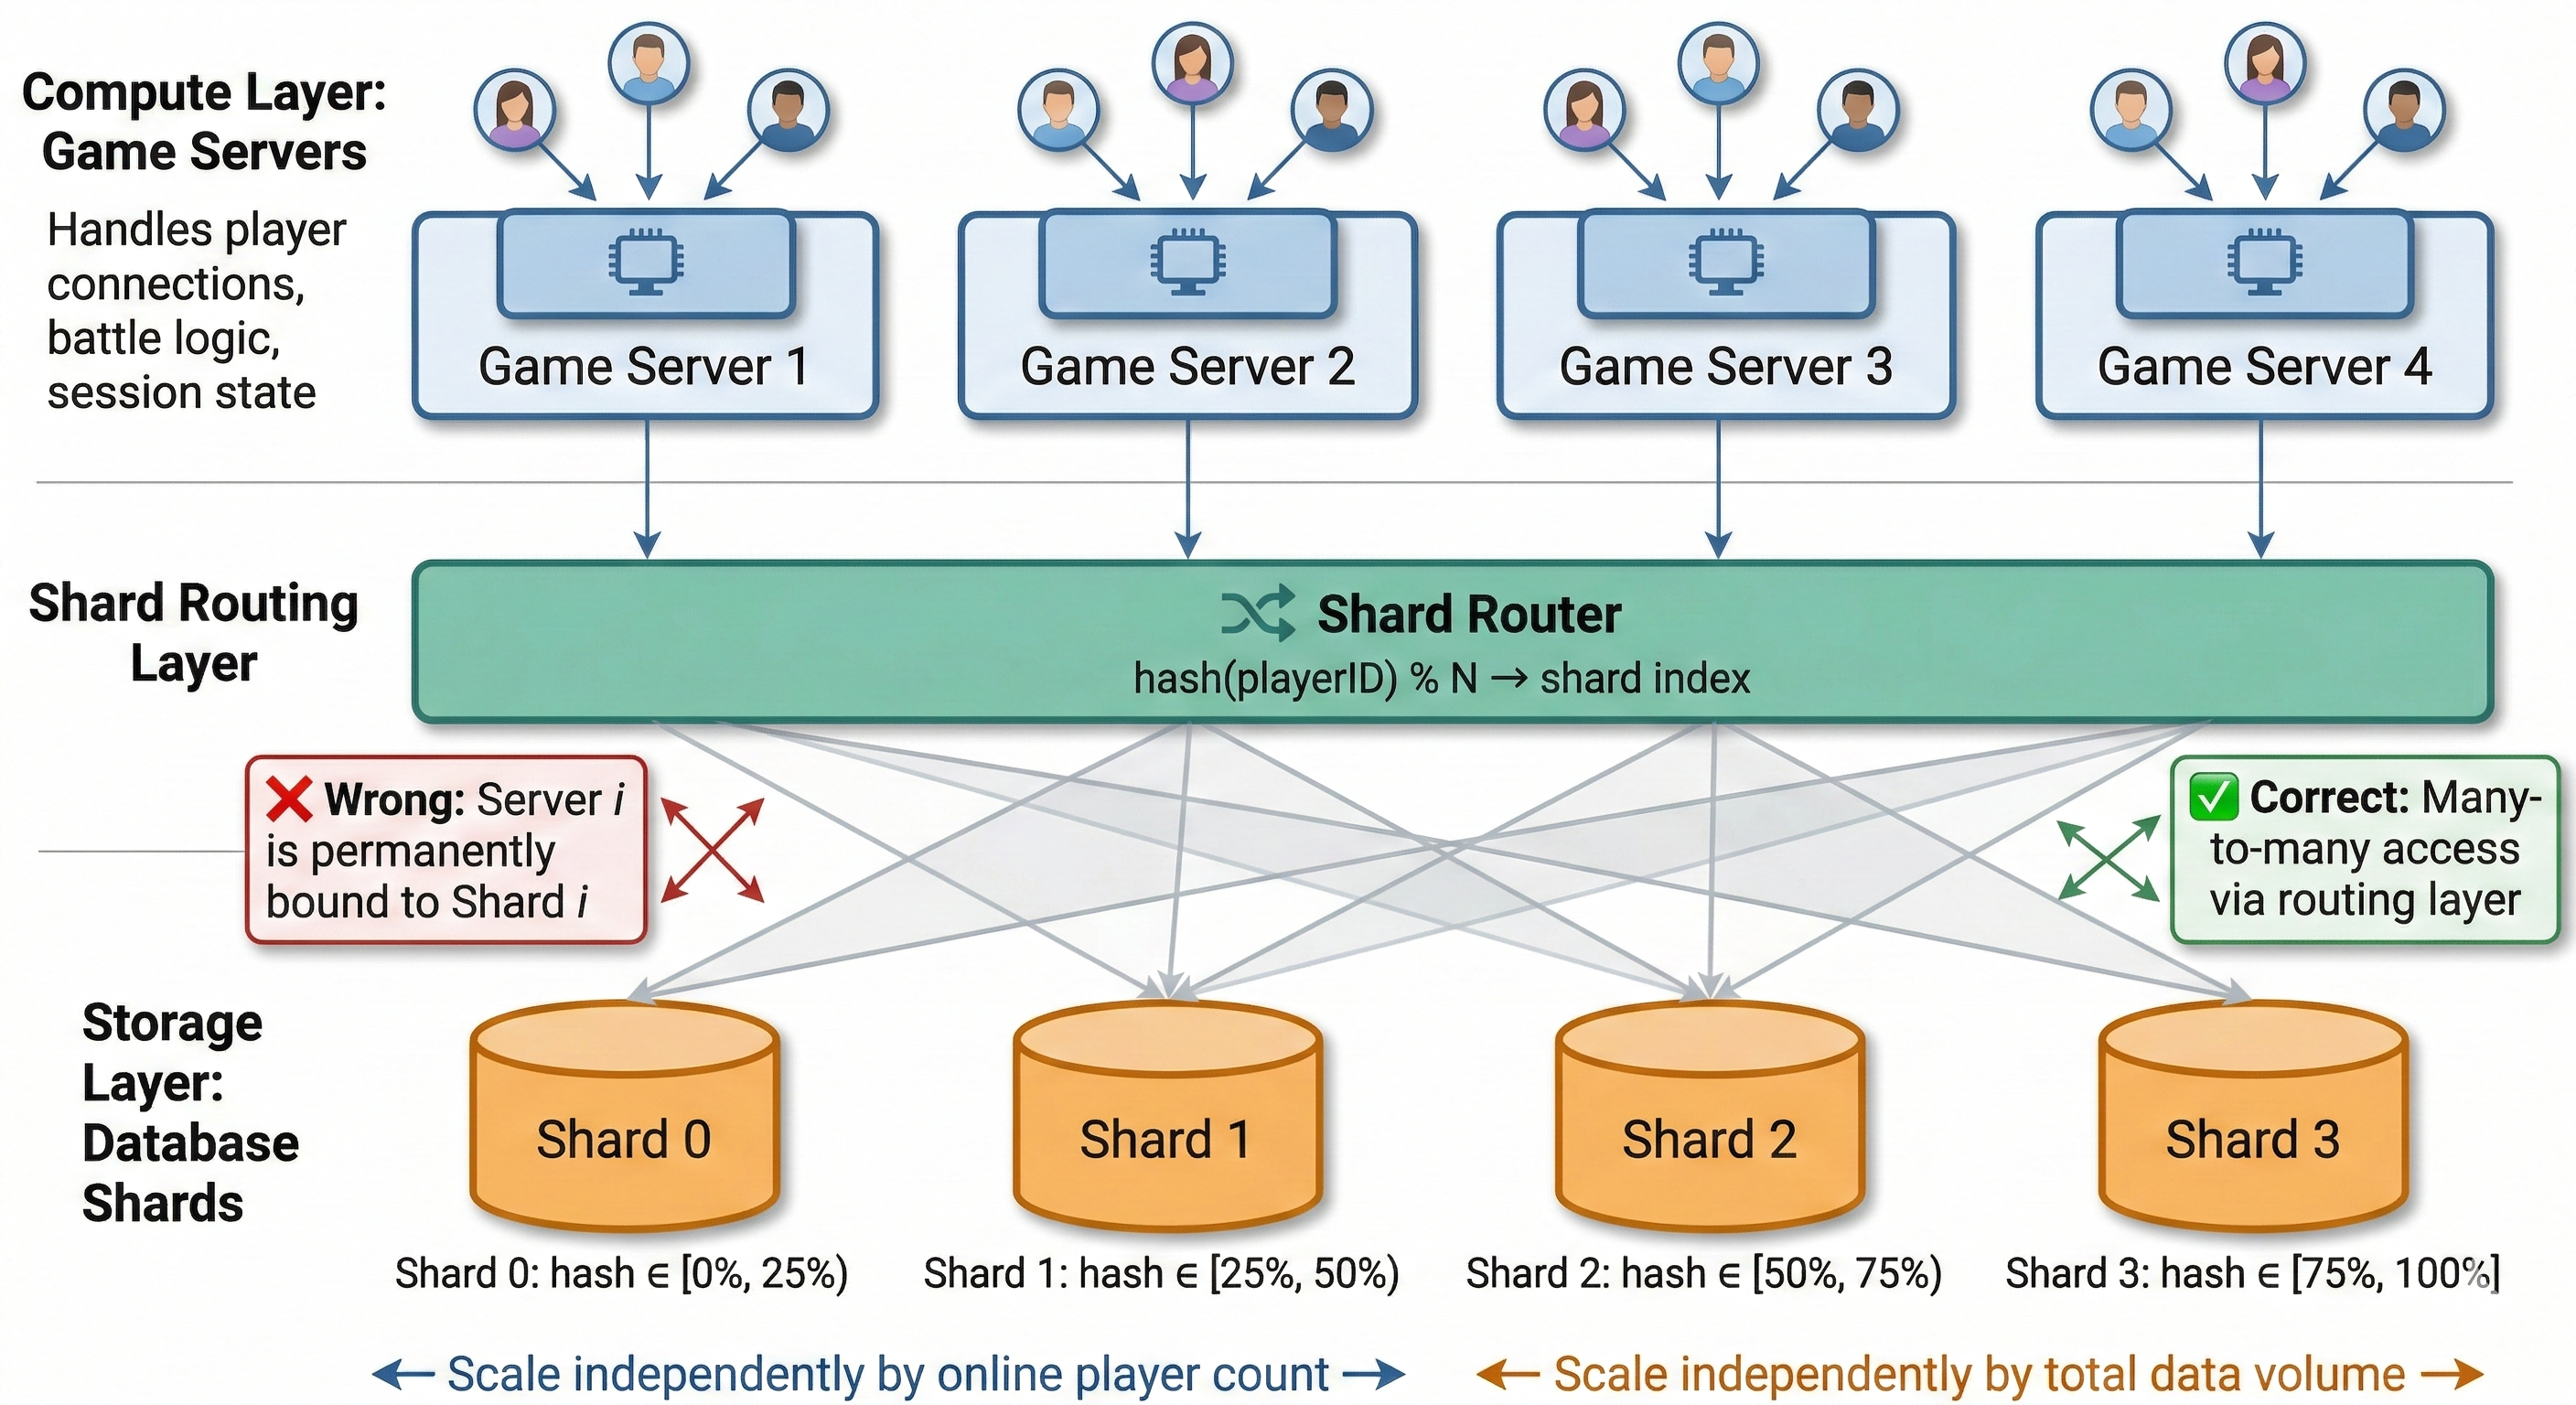
\includegraphics[width=1\linewidth]{figures/sec4/4-server-db.png}
    \caption{游戏服务器（计算层）与数据库分片（存储层）的解耦关系：
    任意游戏服务器均可经由分片路由层访问任意数据库分片，
    两层按各自压力独立水平扩展，不存在一一绑定关系}
    \label{fig:server_db_relationship}
\end{figure}

明确了计算层与存储层的解耦关系之后，计算层扩展的核心问题便清晰地浮现出来：
当我们部署了多台游戏服务器之后，如何让每一台服务器都承担合适的玩家数量和计算压力，
而不是有的服务器人满为患、有的服务器门可罗雀？这正是负载均衡要解决的核心问题。
负载均衡器作为计算层的入口，承担着与分片路由层对等的角色：
分片路由层决定"一条数据库请求去往哪个分片"，
负载均衡器则决定"一个玩家的连接请求去往哪台游戏服务器"。
两者共同构成了整个分布式游戏系统中的两级路由体系，分别守护着存储层和计算层的入口。


\subsubsection{负载不均的表现与根源}

从玩家的视角看，负载不均衡通常表现为两个极端。一方面，有的游戏区服在登录时总是排队，玩家点击"进入游戏"后会看到"当前服务器繁忙，排队中...前方还有 XXX 人"的提示，等待数分钟才能进入；即使成功登录，进入游戏后也感觉卡顿明显——点击匹配按钮后要等很久才能找到对手，战斗过程中画面偶尔会停顿，战斗结算慢，有时甚至会出现"操作超时"的错误提示。另一方面，另一些区服则人迹罕至，玩家登录几乎不需要等待，但进入游戏后发现世界频道冷冷清清，几分钟都没人说话，想要匹配对手时系统提示"当前在线人数较少，匹配时间可能较长"，等了十几分钟也没匹配到人，只能放弃。

这种体验上的巨大差异，归根结底是因为服务器资源没有被合理利用。把这种现象翻译到服务器背后，可以看到一个简单但严重的事实：不同的游戏服务器承载的玩家数量和计算负载差异巨大。假设我们部署了五台游戏服务器，理想情况下每台服务器应该承载大约 20\% 的在线玩家，CPU 使用率都在 60\% 左右，响应时间都在 100 毫秒以内。但现实往往是：服务器 1 承载了 40\% 的玩家，CPU 使用率常年在 90\% 以上，内存占用接近上限，平均响应时间超过 500 毫秒，玩家感受到明显的卡顿；服务器 2 和服务器 3 各承载了 20\% 的玩家，运行状态正常；服务器 4 只有 15\% 的玩家，CPU 使用率只有 40\%，还有大量闲置资源；服务器 5 更是只有 5\% 的玩家，几乎处于空转状态，每天大部分时间都在等待请求。

造成这种不均衡的原因是多方面的。开服时间的差异是最常见的一种：服务器 1 可能是游戏刚上线时开的第一批服务器，大量早期玩家都注册在这个服务器上，形成了庞大的玩家基数和成熟的社交网络；即使后来开了新服务器，老玩家也不愿意迁移，因为他们在老服上有朋友、有公会、有积累。社区效应也会加剧这种不均衡：某个知名主播或游戏公会宣布在服务器 1 上活动，吸引了大量粉丝和玩家涌入；又或者某个服务器因为运气好、氛围好，在玩家社区中形成了"这个服人气旺、高手多"的口碑，进一步吸引新玩家加入，形成正反馈循环。还有技术层面的失误：在没有负载均衡机制的情况下，玩家选服时看到的服务器列表可能是按开服时间或名称排序的，很多玩家会习惯性地选择列表中的第一个或最上面的服务器，导致某几个服务器被优先填满。

这种不均衡不仅造成了资源浪费——服务器 4 和服务器 5 的硬件闲置率极高，相当于花钱买了机器却没有充分使用——更严重的是，它直接影响了玩家的游戏体验。在过载的服务器上，玩家忍受着糟糕的性能；在冷清的服务器上，玩家感受不到多人游戏应有的社交氛围和竞技乐趣。长此以往，过载服务器的玩家会因为体验太差而流失，冷清服务器的玩家会因为找不到对手而离开，最终两边都留不住玩家。

负载均衡的目标，就是通过科学的流量调度策略，让每一台游戏服务器都处于一个相对均衡的工作状态，既不至于过载崩溃，也不会过度闲置。可以把负载均衡器想象成一个站在"入口大厅"的智能引导员：所有新登录的玩家都先来到这个入口，引导员手里有一张实时更新的"服务器状态表"，记录着每台服务器当前的在线人数、CPU 使用率、内存占用、平均响应时间等信息；当一个新玩家到来时，引导员快速查看这张表，找出当前负载最轻、最适合接纳新玩家的服务器，然后将这个玩家的连接请求转发到那台服务器上。整个过程对玩家来说是透明的——玩家只知道自己点击了"开始游戏"，几秒钟后就进入了游戏世界，并不知道背后经历了负载均衡器的选择和转发。

\subsubsection{从轮询到动态调度的策略演进}

要实现负载均衡，最直接的想法是采用轮询策略。假设我们有三台游戏服务器 A、B、C，负载均衡器维护一个简单的计数器，按照固定顺序依次分配玩家：第一个玩家分配到 A，计数器加 1；第二个玩家分配到 B，计数器加 1；第三个玩家分配到 C，计数器加 1；第四个玩家再回到 A，计数器归零后重新开始循环，如此往复。

\begin{tcolorbox}[title=轮询策略的核心逻辑]
\begin{lstlisting}[
    language=go,
    basicstyle=\ttfamily\footnotesize,
    aboveskip=0pt, belowskip=0pt,
    lineskip=-1pt,
    commentstyle=\color{gray},
    keywordstyle=\color{blue}\bfseries,
    breaklines=true
]
// 选择下一个服务器（轮询）
current = (current + 1) % numServers
return servers[current]
\end{lstlisting}
\end{tcolorbox}

这种策略的优点在于规则清晰、实现简单，代码量很少，逻辑一目了然，不需要收集任何服务器的实时状态信息，不需要复杂的计算和判断。而且从统计学的角度看，如果玩家登录是随机分布的，经过足够长的时间，每台服务器理论上都会接收到大致相同数量的新玩家——假设有 10000 个玩家陆续登录，三台服务器最终各自会分配到约 3333 个玩家，偏差不会太大。

但轮询策略有一个明显的局限：它只关心"过去分配了多少人"，而完全不关心"现在每台服务器到底有多忙"。这种"盲目"的分配方式在某些情况下会导致严重的问题。假设服务器 A 因为历史原因已经承载了 5000 个老玩家，这些老玩家虽然没有在刚才的轮询分配中被计入，但他们确实占用着服务器 A 的 CPU、内存和网络资源。此时，如果继续按照轮询规则将新玩家平均分配给三台服务器，服务器 A 就会承受双重压力：5000 个老玩家加上新分配来的约 3333 个新玩家，总共 8333 个玩家；而服务器 B 和 C 可能只有新分配的 3333 个玩家。结果是服务器 A 的负载远高于 B 和 C，性能急剧下降，玩家体验变差。

更极端的情况是，某台服务器正在处理突发的高负载事件。比如，服务器 A 上的两个大型公会正在进行一场 100 人规模的公会战，这场战斗涉及大量的位置同步、技能计算、伤害结算，CPU 使用率已经飙升到 95\%，响应时间从平时的 50 毫秒增加到了 800 毫秒。但轮询策略对这一切毫无感知，它仍然会按照固定的顺序，将下一批新登录的玩家中的三分之一分配给服务器 A。这些新玩家刚登录就会感受到明显的延迟和卡顿，甚至可能因为服务器过载而连接失败。与此同时，服务器 B 和 C 可能相对空闲，CPU 使用率只有 30\%，完全有余力接纳更多玩家，但轮询策略并不会将更多玩家导向它们。

为了克服这个问题，我们需要让负载均衡器具备"感知"能力——它需要知道每台服务器当前的真实负载状况，并根据这些信息做出更智能的分配决策。具体做法是让每台游戏服务器定期向负载均衡器报告自己的当前状态，这个报告过程通常通过心跳机制来实现：每台游戏服务器每隔一段时间（比如每 5 秒）向负载均衡器发送一条心跳消息，消息中包含该服务器的关键指标，包括在线玩家数、CPU 使用率、内存占用率、平均响应时间、当前活跃战斗数等。

\begin{tcolorbox}[title=服务器心跳上报的关键数据]
\begin{lstlisting}[
    language=go,
    basicstyle=\ttfamily\footnotesize,
    aboveskip=0pt, belowskip=0pt,
    lineskip=-1pt,
    commentstyle=\color{gray},
    keywordstyle=\color{blue}\bfseries,
    breaklines=true
]
type ServerStatus struct {
    ServerID      string
    OnlinePlayers int     // 在线玩家数
    CPUUsage      float64 // CPU使用率 (0-100)
    MemUsage      float64 // 内存使用率 (0-100)
    AvgRespTime   int     // 平均响应时间（毫秒）
    ActiveBattles int     // 活跃战斗数
}
// 每5秒发送一次心跳到负载均衡器
\end{lstlisting}
\end{tcolorbox}

负载均衡器收集到这些信息之后，会在内存中维护一张"服务器状态表"，记录每台服务器的最新状态。游戏服务器启动时会创建一个定时器，每隔固定时间间隔读取自身的运行指标，将这些指标打包成一条消息发送给负载均衡器；负载均衡器收到心跳后，更新对应服务器在状态表中的记录，并记录心跳的接收时间，用于后续的健康检查。

有了这些实时状态信息，负载均衡器就可以做出更明智的决策。最简单的一种动态策略是"最少连接优先"：负载均衡器会优先将新玩家分配到当前在线玩家数最少的服务器上。这种策略的直觉很简单——玩家数少的服务器通常意味着负载较轻，还有余力接纳更多玩家；而玩家数多的服务器可能已经接近满负载，不应该继续向它分配新玩家。实现时，负载均衡器在收到新玩家的连接请求后，遍历服务器状态表，找出在线玩家数最少的那台服务器，将玩家的连接转发给它。

最少连接策略相比轮询策略有了显著的改进。当某台服务器因为历史原因积累了大量玩家时，负载均衡器会自动减少向它分配新玩家，转而将更多新玩家导向那些相对空闲的服务器，从而实现负载的动态平衡。随着时间推移，各台服务器的玩家数量会逐渐趋于一致，不再出现某台服务器人满为患、另一台服务器门可罗雀的极端情况。

但"最少连接"也不是万能的。玩家数量并不总是等同于计算负载，这是一个非常重要但容易被忽视的事实。我们可以构造这样一个场景来说明问题：服务器 A 当前在线 2000 个玩家，服务器 B 当前在线 3000 个玩家。从玩家数量上看，服务器 A 明显更少，按照最少连接策略，下一个玩家应该被分配到服务器 A。但实际情况可能是：服务器 A 上的 2000 个玩家中有 1500 个正在进行激烈的实时对战，每场战斗都需要频繁的位置同步、技能判定、伤害计算，CPU 使用率已经达到 85\%；而服务器 B 上的 3000 个玩家中有 2000 个处于挂机状态（可能在等待体力恢复、在城镇闲逛、或者打开了游戏但没有实际操作），只有 1000 个在进行战斗，CPU 使用率只有 50\%。在这种情况下，如果继续将新玩家分配给服务器 A，很可能导致它过载；而服务器 B 虽然玩家更多，但实际上还有充足的计算资源可以接纳更多玩家。

这个例子揭示了一个关键问题：玩家数量是一个简单但粗糙的指标，它无法准确反映服务器的真实负载。要做出更精准的负载评估，我们需要综合考虑多个维度的指标：在线玩家数（反映需要维护的连接数和会话状态数量）、CPU 使用率（反映计算压力，战斗计算、路径寻找、AI 决策等都会消耗 CPU）、内存占用率（反映内存使用情况，过高可能触发系统回收机制）、平均响应时间（反映整体性能表现，是玩家最直接感受到的指标）、活跃战斗数（反映当前的业务负载强度，在对战游戏中这是计算密集型任务）。

我们可以为每个指标设置一个权重，然后将各个指标的数值按权重加总，得到一个综合负载值。权重的设置需要根据具体的游戏特性和硬件配置来调整。例如，对于我们的对战游戏，战斗计算是主要的性能瓶颈，CPU 使用率和活跃战斗数应该占更高的权重；而对于社交类游戏，在线玩家数和网络带宽可能更重要。

\begin{tcolorbox}[title=综合负载值的计算方法]
\begin{lstlisting}[
    language=go,
    basicstyle=\ttfamily\footnotesize,
    aboveskip=0pt, belowskip=0pt,
    lineskip=-1pt,
    commentstyle=\color{gray},
    keywordstyle=\color{blue}\bfseries,
    breaklines=true
]
// 计算综合负载值（0-100，值越高负载越重）
loadScore = playerScore*0.2 + cpuScore*0.3 + memScore*0.2 
          + respTimeScore*0.2 + battleScore*0.1

// 选择负载最低的服务器
bestServer = findMinLoadScore(allServers)
\end{lstlisting}
\end{tcolorbox}

计算时，首先将各项指标归一化到 0-100 的范围（比如假设 5000 人为玩家数满载，1000 毫秒为严重延迟的响应时间），然后按照预设的权重进行加权求和，最终得到一个 0-100 的综合负载值，数值越高表示负载越重。负载均衡器在分配玩家时，选择综合负载值最低的服务器。

通过这种加权负载评估，负载均衡器可以更全面地了解每台服务器的真实状况。即使某台服务器的在线玩家数较少，但如果它的 CPU 使用率很高、活跃战斗数很多，综合负载值仍然会比较高，负载均衡器就不会继续向它分配新玩家；相反，如果另一台服务器虽然玩家数较多，但大部分玩家处于空闲状态，各项指标都比较健康，综合负载值较低，负载均衡器就会优先将新玩家分配给它。

% \begin{figure}[htbp]
%     \centering
%     % 图片描述：不同负载均衡策略的对比示意图
%     % 三个子图水平排列：
%     % 左图：轮询策略
%     %   - 三台服务器A、B、C的柱状图，高度相同（各33.3%）
%     %   - 标注"平均分配，但未考虑实际负载"
%     % 中图：最少连接策略
%     %   - 三台服务器的柱状图，高度根据玩家数动态调整
%     %   - 服务器A: 40%（老玩家多），服务器B: 35%，服务器C: 25%（新开服）
%     %   - 标注"根据玩家数动态调整"
%     % 右图：加权负载策略
%     %   - 三台服务器的柱状图，高度根据综合负载值调整
%     %   - 每个柱子分段显示不同指标的贡献（CPU、内存、玩家数等）
%     %   - 服务器A综合负载85分，服务器B: 60分，服务器C: 45分
%     %   - 标注"多维度综合评估"
%     % 所有文字使用简体中文
%     \caption{不同负载均衡策略的分配效果对比}
%     \label{fig:load_balancing_comparison}
% \end{figure}

\subsubsection{硬件差异与动态权重}

在实际部署中，还有一个现实问题需要考虑：不同的游戏服务器可能拥有不同的硬件配置。在游戏运营的早期阶段，我们可能只有几台配置一般的服务器（比如 8 核 CPU、32GB 内存）；随着玩家增长，我们陆续采购了一些性能更强的服务器（比如 16 核 CPU、64GB 内存）；到了后期，可能还会租用云服务器，这些云服务器的配置可能又各不相同。如果采用完全均等的负载均衡策略，不考虑硬件差异，就会导致一个问题：配置较低的服务器更容易过载，而配置较高的服务器则没有充分发挥性能优势。

假设服务器 A 是老旧的 8 核服务器，承载能力大约是 2000 个并发玩家；服务器 B 是新购的 16 核服务器，承载能力大约是 4000 个并发玩家。如果负载均衡器简单地将玩家平均分配，最终两台服务器各承载 3000 个玩家，结果就是：服务器 A 严重过载（超出承载能力 50\%），CPU 使用率常年在 95\% 以上，玩家体验很差；而服务器 B 还有余力（只用了 75\% 的承载能力），但由于负载均衡器的限制，没能接纳更多玩家。

为了解决这个问题，我们可以为每台服务器设置一个权重值。权重值通常根据服务器的硬件配置来确定，配置越高、承载能力越强的服务器，权重值越大。负载均衡器在分配玩家时，会按照权重比例进行分配，让硬件资源得到更充分的利用。例如，如果服务器 A（8 核）权重设为 1，服务器 B（16 核）权重设为 2，服务器 C（24 核）权重设为 3，那么在长期运行中，三台服务器接收到的玩家数量会大致符合 1:2:3 的比例，服务器 A 接收约 16.7\% 的流量，服务器 B 接收约 33.3\%，服务器 C 接收约 50\%。通过权重机制，我们可以让高配置服务器承担更多的玩家，低配置服务器承担较少的玩家，使得每台服务器都工作在合理的负载水平上，既不会因为配置低而过载，也不会因为配置高而闲置。

但权重也不应该是固定不变的。随着服务器运行时间的增长，硬件可能会老化，性能有所下降；或者某台服务器上积累了大量的历史数据（比如战斗记录、聊天日志），导致数据库查询变慢；又或者某台服务器因为网络拓扑的原因，与部分玩家之间的延迟较高。这些因素都会影响服务器的实际承载能力。因此，更好的做法是引入动态权重调整机制：负载均衡器不仅在启动时从配置中读取静态权重，还会根据服务器的实时表现动态调整权重。如果某台服务器虽然硬件配置高，但实际表现不佳（比如平均响应时间持续偏高），负载均衡器会逐步降低它的权重，减少向它分配的流量；反之，如果某台服务器表现优异，权重可以适当提升。调整的方式可以是：每次收集到服务器状态信息后，根据综合负载值与目标负载值的差距，微调该服务器的权重——如果综合负载持续高于目标值，权重逐步下降；如果持续低于目标值，权重逐步上升。这种微调是渐进的、平滑的，避免权重的剧烈波动导致流量分配不稳定。

\subsubsection{健康检查与故障隔离}

除了动态权重，负载均衡器还需要建立健康检查机制。所谓健康检查，就是负载均衡器定期向每台游戏服务器发送探测请求，检测服务器是否正常响应。这个探测可以是一个简单的 HTTP 请求（比如访问一个专门的健康检查端点），也可以是一个轻量级的 RPC 调用。服务器收到探测请求后，应该快速返回一个包含自身状态信息的响应，表明自己还活着并且运行正常。响应中不仅包含一个简单的"我还活着"的标志，还可以包含一些关键指标的快照，比如当前 CPU 使用率、是否能正常连接数据库、是否有严重的错误日志等。

如果某台服务器连续多次健康检查失败——可能是进程崩溃、可能是网络中断、可能是硬件故障——负载均衡器就会将这台服务器标记为"不可用"，暂停向它分配新玩家。这个标记过程通常会设置一个失败次数阈值，避免因为偶发的网络抖动而误判。比如，只有当连续三次健康检查都失败时，才将服务器标记为不可用；而当服务器恢复正常、连续三次健康检查都成功时，才将它重新标记为可用。标记为不可用的服务器会被从分配池中移除，新玩家的连接请求不会再被转发到这台服务器，所有流量都会被导向其他健康的服务器。

对于已经连接到故障服务器的玩家，负载均衡器还需要考虑如何处理。最简单的做法是让这些玩家的连接自然断开，等他们重新登录时再分配到其他健康的服务器上。但这种方式对玩家体验影响较大——正在进行战斗的玩家会突然掉线，正在浏览背包的玩家会看到"连接丢失"的错误。更好的做法是引入连接迁移机制：当负载均衡器检测到某台服务器不健康时，会向该服务器上的所有玩家发送一条"服务器维护"的通知，引导他们在未来的某个时间点（比如当前战斗结束后、或者 5 分钟后）重新连接到其他服务器。这样可以给玩家一个缓冲期，避免突然的连接中断。待故障服务器恢复正常后，负载均衡器会重新将其纳入分配池。但不应该立即将大量玩家分配给刚恢复的服务器，因为它可能还处于不稳定状态，或者需要时间来预热（比如加载缓存、建立数据库连接池等）。更稳妥的做法是逐步恢复：刚恢复时，只分配少量玩家；观察一段时间后，如果服务器表现稳定，再逐步增加分配的流量，直到恢复到正常的权重比例。

\subsubsection{运行时动态迁移应对突发负载}

负载均衡不仅仅发生在玩家刚登录的那个瞬间。在游戏运行过程中，各台服务器的负载可能因为各种
原因发生剧烈波动。最典型的情况是突发事件：某个服务器上正在举行一场大型公会战，
参战的 200 个玩家几乎同时上线并进入战场，短时间内该服务器的活跃战斗数从 50 场飙升到 150 场，
CPU 使用率从平时的 50\% 跃升到 90\%，平均响应时间从 100 毫秒增加到 600 毫秒。
与此同时，另一些服务器可能相对空闲——也许是因为时区差异导致欧洲玩家还没上线，
也许只是这一批玩家碰巧都在做日常任务、没人打排位赛。
如果仅靠"不再向过载服务器分配新玩家"这一策略，只能防止问题进一步恶化，
但无法缓解已经发生的过载——过载服务器上那批老玩家还在继续游戏，CPU 仍然居高不下。
为此，一些高级的负载均衡系统会引入运行时的动态迁移机制，
主动将过载服务器上的部分玩家迁移到相对空闲的服务器上。

动态迁移的第一个问题是"迁移谁"。并不是所有玩家都适合在运行时被迁移——
正在战斗中的玩家、正在进行购买或开箱等关键操作的玩家，迁移会打断他们的状态，
造成不良体验甚至数据丢失。更合适的迁移对象是那些暂时不活跃的玩家：
超过 10 分钟没有任何操作的挂机玩家、刚结束战斗正在查看战绩的玩家、
在城镇闲逛或浏览商店的玩家。这些玩家当前的游戏状态较为简单，
迁移时需要同步的数据量小，中断带来的影响也最轻微。

动态迁移的第二个、也是更核心的问题是"怎么迁移"。
这里所说的迁移，并非重启连接这么简单——玩家登录游戏后，
服务器内存中保存着他当前的完整游戏状态：角色在地图上的位置、当前血量和技能冷却、
进行中的任务进度、战斗中的仇恨列表，乃至玩家客户端的网络连接上下文。
如果只是断开连接然后让玩家重新登录，固然可行，但玩家体验很差——
相当于强制把玩家踢出再拉回来。真正的状态热迁移要求：在玩家几乎无感知的前提下，
将这份内存中的活跃状态完整地搬到另一台服务器上，并由目标服务器无缝接管后续的服务。
根据如何处理"迁移期间源服务器仍在运行、状态仍在变化"这一核心矛盾，
主要有以下三种方案，复杂度和效果依次递进。

\paragraph{方案一：停止复制法（Stop-and-Copy）}

最直接的做法是"先停、再搬、再启"，即停止复制法（Stop-and-Copy），
如图~\ref{fig:migration_stop_copy} 所示。
迁移开始时，源服务器立即停止处理该玩家的所有请求，
将玩家的完整会话状态序列化为一个可传输的数据结构，
通过网络传输到目标服务器，目标服务器反序列化后恢复玩家会话，
最后原服务器关闭连接，玩家的客户端重连到目标服务器。
这种方案的优点是实现极为简单：停机期间状态不再变化，不存在任何数据竞争，
序列化的快照完全一致，目标服务器恢复时无需任何额外协调。
缺点也同样明显：玩家在整个传输过程中处于完全停服状态，
停机时长与需要迁移的状态数据量成正比——
对于一个状态复杂的玩家（身处大型公会战、同屏数十个技能特效全部需要同步），
全量序列化和传输可能耗时数秒甚至更长，玩家会明显看到"连接断开"或"转圈等待"。
因此，停止复制法通常只适用于离线维护窗口或玩家处于彻底挂机状态的场景，
不适合作为生产环境中的主动负载均衡手段。

\begin{figure}[htbp]
    \centering
    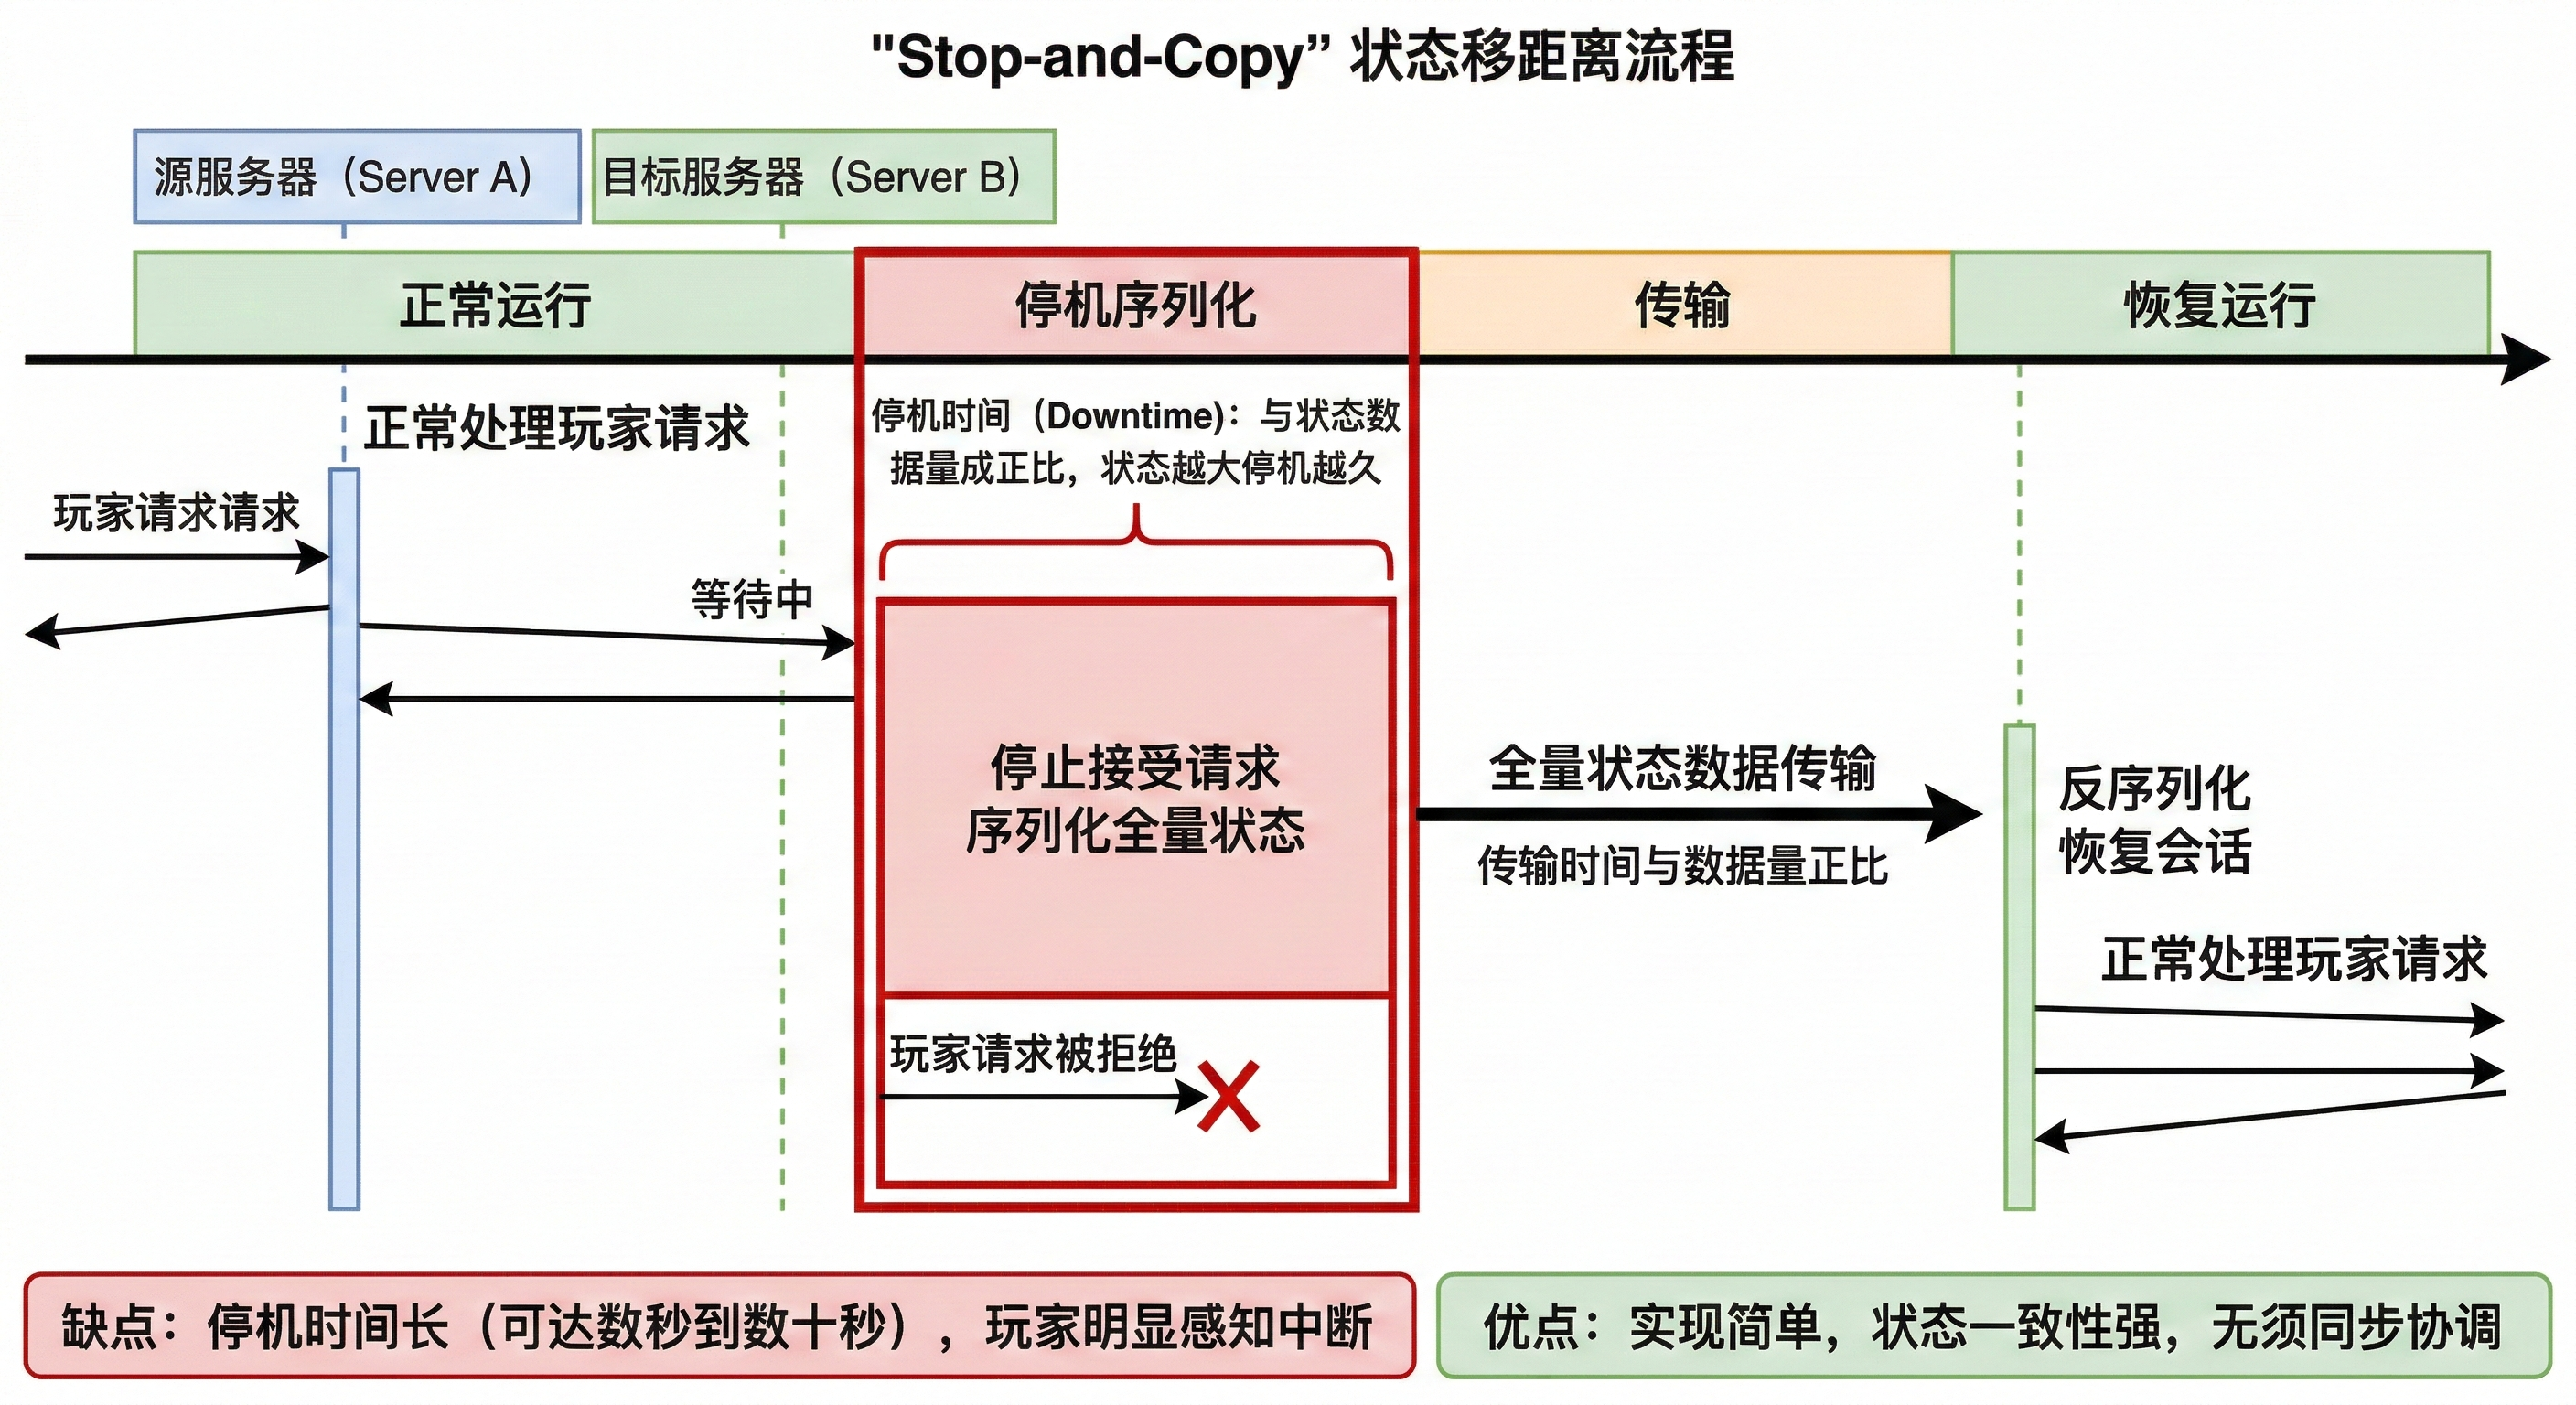
\includegraphics[width=1\linewidth]{figures/sec4/4-migrate-stop.png}
    \caption{停止复制法（Stop-and-Copy）：源服务器停机后传输全量状态，
    停机时间与状态数据量成正比，玩家会明显感知到连接中断}
    \label{fig:migration_stop_copy}
\end{figure}

\paragraph{方案二：预复制法（Pre-Copy）}

为了缩短玩家感知到的停机时间，可以把大部分数据的传输提前到停机之前完成，
这就是预复制法（Pre-Copy），如图~\ref{fig:migration_precopy} 所示。
其核心思路是：在源服务器仍然运行的同时，持续地将玩家状态的内存快照传输到目标服务器；
每一轮传输结束后，追踪本轮期间哪些内存页被修改过（称为"脏页"，Dirty Pages），
再在下一轮只传输这些脏页，逐轮迭代，直到每轮的脏页数量收敛到足够小；
最后才进行一次极短暂的停机，将最后一批脏页和 CPU 寄存器状态传输过去，
完成最终切换。
这里有个关键直觉值得理解：游戏服务器的内存并不会在每一秒内把所有状态全部修改一遍，
绝大多数玩家数据（已完成的任务记录、背包里不在使用的装备、离线好友列表等）
在单次传输间隔内根本不会被修改，只有当前正在活跃变化的那部分状态（当前帧的位置、血量）
才会产生新的脏页。随着迭代轮次增加，每轮需要重传的脏页越来越少，
最终只需在极短的窗口内传输最后一批脏页就能完成切换，
停机时间通常可以从秒级压缩到百毫秒级甚至更低。
预复制法的代价是总传输量会超过全量状态大小——部分脏页在多轮迭代中被反复传输，
网络带宽的消耗高于停止复制法；对于那些高频修改的"热页"（比如每帧都在变化的角色位置），
无论迭代多少轮都无法在停机前完全收敛，最终仍然要在停机阶段传输，
这构成了预复制法停机时间的理论下界。

\begin{figure}[htbp]
    \centering
    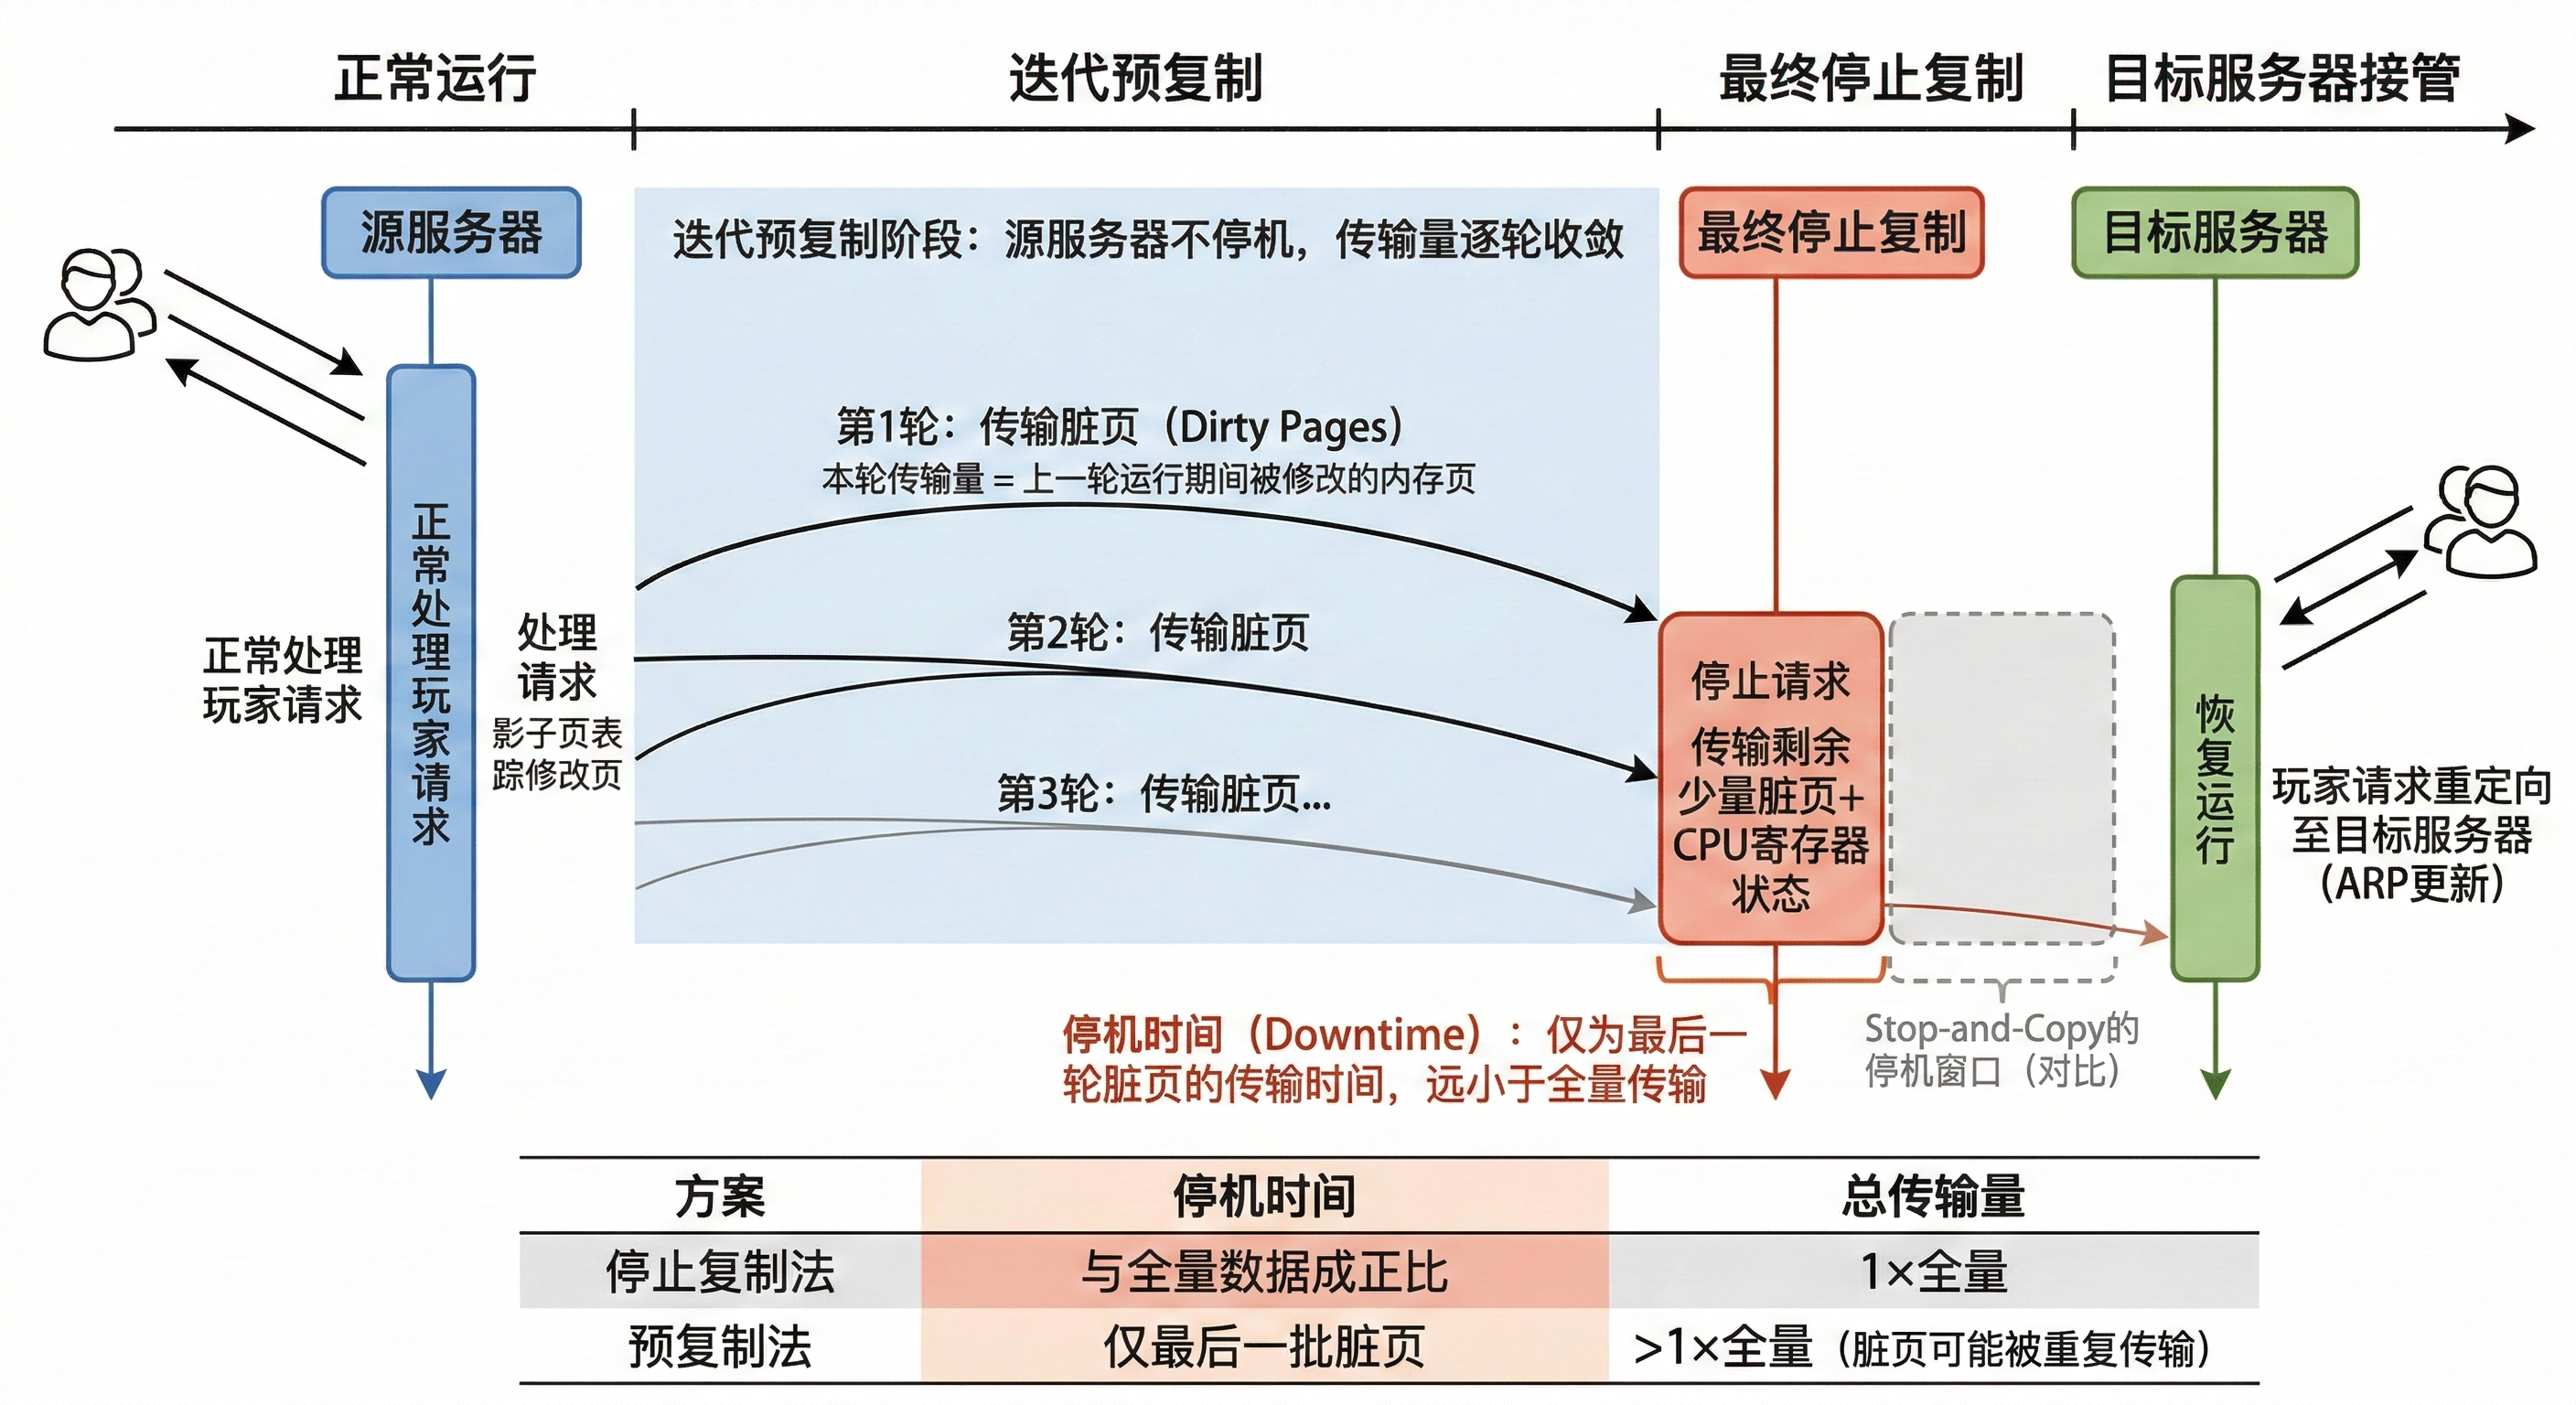
\includegraphics[width=1\linewidth]{figures/sec4/4-migrate-precopy.png}
    \caption{预复制法（Pre-Copy）：源服务器持续运行，迭代传输脏页直至收敛，
    最终仅需极短停机传输剩余脏页；停机时间远小于停止复制法，但总传输量更大}
    \label{fig:migration_precopy}
\end{figure}

\paragraph{方案三：按优先级分波迁移（Wave-Based Migration）}

停止复制法和预复制法都来源于虚拟机迁移领域，将玩家所在的整个服务器进程视为迁移单元，
迁移的是完整的内存镜像。但对于游戏服务器来说，并不是所有内存状态对玩家的即时体验
都同等重要——在玩家切换服务器的那一帧，最关键的只是角色位置、动画帧、生命值这几项数据；
场景中视野外的敌人状态、已完成战斗的历史记录，晚几百毫秒同步完全没有问题。
这一洞察催生了面向游戏场景的分波迁移法（Wave-Based Migration），
如图~\ref{fig:migration_wave} 所示。

分波迁移的流程分为三个阶段。第一步是预热阶段：在迁移实际发生之前，
目标服务器提前收到指令，加载该玩家所在关卡的静态资源（地图、关卡配置、
通用对象列表），这一步可以在玩家完全无感知的情况下在后台完成，
将原本需要数秒的资源加载时间从关键路径上彻底移除。
第二步是触发与第一波同步：当迁移正式触发时，
源服务器向目标服务器发送第一波状态——仅包含对即时玩家体验至关重要的少量数据：
玩家角色的当前位置与朝向、精确到帧的动画状态、当前血量与技能冷却。
由于第一波数据极小（通常在数 KB 以内），目标服务器几乎立刻就能据此渲染出
对玩家而言视觉连续的第一帧画面并发回客户端，使得玩家感知到的服务中断时间
压缩至不足 25 毫秒——在 30 帧/秒的游戏中，这甚至不到一帧的时间。
第三步是后续波次的静默同步：在客户端已经恢复正常接收帧的同时，
源服务器继续将视野范围内的其他对象状态（第二波）、视野外的全局对象状态（第三波）
逐步传输给目标服务器，目标服务器在后台完成这些数据的恢复，整个过程对玩家完全透明。

\begin{tcolorbox}[title=按优先级分波迁移的核心逻辑]
\begin{lstlisting}[
    language=go,
    basicstyle=\ttfamily\footnotesize,
    aboveskip=0pt, belowskip=0pt,
    lineskip=-1pt,
    commentstyle=\color{gray},
    keywordstyle=\color{blue}\bfseries,
    breaklines=true
]
// 阶段0：提前预热目标服务器（后台静默执行）
targetServer.PreloadStaticAssets(player.CurrentLevel)

// 触发迁移：发送触发信号，源服务器发出最后一帧
triggerMigration(sourceServer, targetServer, player)

// 第一波：最小关键状态（毫秒级，决定玩家感知的中断时长）
wave1 := PlayerCriticalState{
    Position:      player.Position,
    AnimatorFrame: player.AnimatorFrame,  // 精确到帧，保证动画连续
    HP:            player.HP,
    CameraState:   player.Camera,
}
targetServer.ApplyWave(1, wave1)
// 目标服务器立即渲染第一帧并发回客户端，服务恢复

// 第二波：视野内其他对象（后台同步，玩家已恢复正常游戏）
wave2 := collectVisibleObjects(player)
targetServer.ApplyWave(2, wave2)

// 第三波：视野外全局对象（后台静默，完全无感）
wave3 := collectAllRemainingObjects(player)
targetServer.ApplyWave(3, wave3)

// 源服务器确认迁移完成，清理该玩家的会话和内存
sourceServer.CleanupPlayer(player)
\end{lstlisting}
\end{tcolorbox}

\begin{figure}[htbp]
    \centering
    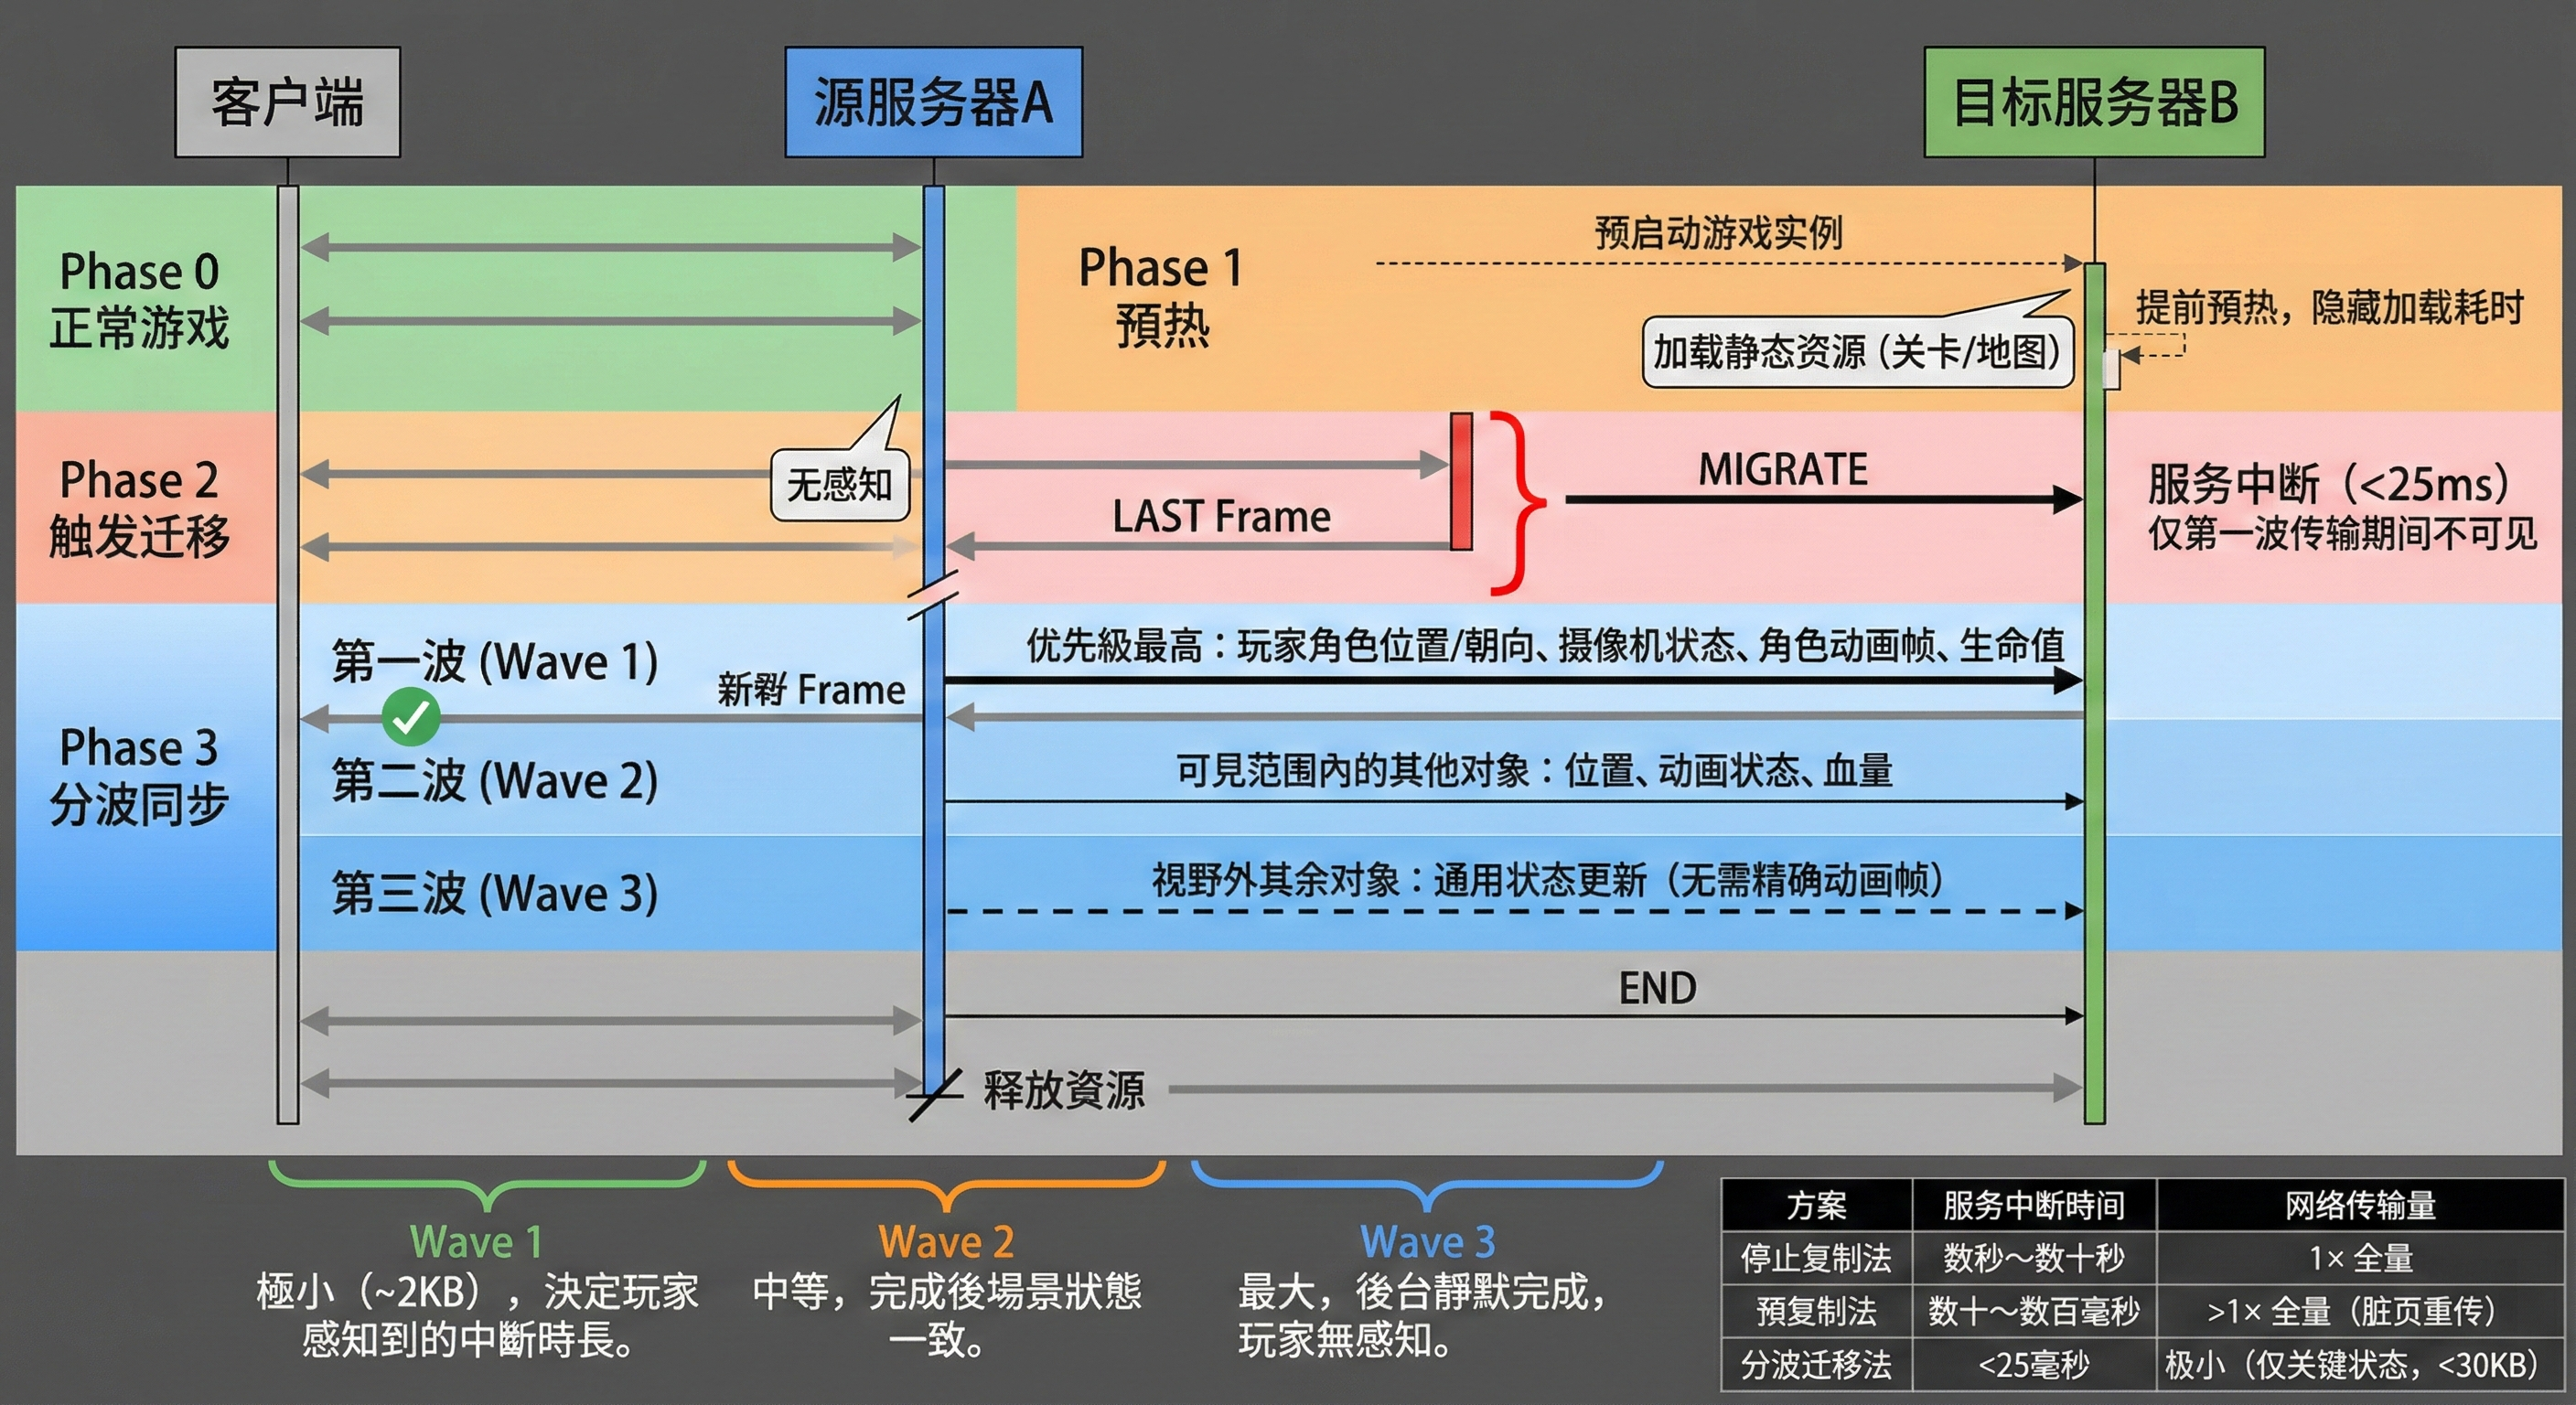
\includegraphics[width=1\linewidth]{figures/sec4/4-migrate-wave.png}
    \caption{按优先级分波迁移：第一波仅传输角色位置、动画帧等极少量关键数据（<30KB），
    使玩家服务中断低于 25ms；后续波次在客户端已恢复正常后于后台静默完成，
    总传输量远小于全量内存复制}
    \label{fig:migration_wave}
\end{figure}

三种方案的本质区别在于如何权衡停机时间、传输量和实现复杂度。
停止复制法以最简单的实现换来最长的停机时间，适合维护窗口或离线场景。
预复制法通过迭代传输脏页大幅压缩停机时间，但总传输量更大，
适合通用服务器迁移场景，VMware 的 vMotion 和 Xen 的虚拟机热迁移均采用此思路。
分波迁移法则针对游戏场景的领域特性——状态有明确的重要性层次——
将停机时间压缩到单帧以内，代价是需要开发者在引擎层面对游戏状态进行优先级分类，
实现复杂度最高，但玩家体验最佳。

无论采用哪种迁移方案，在工程实践中都需要配合两项约束来防止迁移本身成为新的负担。
其一是迁移冷却期：同一台服务器在执行一次迁移后需要等待一段时间（如 30 分钟）
才能再次触发，避免迁移操作频繁进行，给服务器间网络带宽带来持续压力。
其二是单次迁移的玩家数量上限：每次迁移不宜超过一定规模（如 100 人），
防止目标服务器因短时间内涌入大量新会话而出现新的过载，
使得原本的缓解措施反而制造了新的热点。



\subsection{跨服擂台：分布式环境下的玩家交互}

当数据被拆分、负载被均衡之后，游戏世界从"一台大服务器"演化成了"许多协同工作的服务器"：不同机器上运行着不同的游戏区服，每一台都在忙碌地照看自己负责的那一片玩家群体。在这样的世界里，一个自然的想法会浮现出来：既然玩家已经被分散到多个服务器上，能不能让他们在某一个玩法里"跨服相遇"？

这个想法并非凭空而来，而是源于分布式架构本身带来的一个副作用。当我们为了承载更多玩家而将他们分散到多台服务器时，无意中也在玩家群体之间竖起了一道道无形的墙——服务器 1 的玩家只能看到服务器 1 的其他玩家，服务器 2 的玩家只能看到服务器 2 的其他玩家，彼此之间完全隔离，就像生活在平行宇宙中。对于一些需要大量玩家参与的玩法（比如公会战、世界 BOSS），这种隔离问题不大；但对于竞技性的 PvP 玩法，这种隔离会带来一些负面影响：人少的服务器玩家找不到对手，人多的服务器玩家总是遇到同样的老面孔，新鲜感和竞技性都会下降。

跨服擂台，正是这样一种试图打破服务器壁垒、把分布式架构转化为玩法优势的尝试。它的核心理念是：虽然玩家的数据分散存储在不同的数据库分片上，虽然玩家平时连接的是不同的游戏服务器，但在"擂台"这个特定的玩法场景中，我们可以让所有服务器的玩家汇聚到一个统一的竞技平台上，在这里他们可以看到来自全区全服的对手，可以挑战任何一个报名参赛的玩家，不再受服务器边界的限制。本节将通过这个跨服擂台案例，展示分布式环境下如何实现玩家交互、如何保证全局一致性，以及如何设计一个可靠的协调机制。

\subsubsection{跨服交互的设计思路与核心挑战}

在传统的单服架构中，玩家只能与同一台服务器上的其他玩家互动。这种限制在一定程度上保证了系统的简单性——所有相关的数据都在同一个数据库中，所有相关的计算都在同一台服务器上，不需要考虑跨机器通信、数据同步、一致性保证这些复杂问题。但它也带来了一个显而易见的弊端：服务器之间的玩家群体是割裂的。

这种割裂在不同规模的服务器上会产生不同的问题。对于玩家数量较少的服务器——可能是新开的服务器，也可能是老服务器上的玩家逐渐流失——活跃玩家之间很快就会互相熟悉，每天匹配到的对手总是那么几个人。久而久之，玩家会感到竞技的新鲜感在下降，因为对手的打法、战力、习惯都已经了如指掌，缺少了探索和未知的乐趣。更严重的是，当活跃玩家数量低于某个阈值时，匹配系统可能需要很长时间才能找到一个合适的对手，甚至完全匹配不到人，玩家只能放弃这个玩法。对于玩家数量众多的服务器，虽然不存在"找不到人"的问题，但也有另一种困扰：人多的服务器往往竞争更激烈，想要在排行榜上占据靠前的位置，需要投入大量的时间和精力，甚至需要氪金强化装备。而在人少的服务器上，同样的战力可能轻松登顶。这种服务器之间的难度差异，会让玩家产生"选错服务器"的遗憾感。

跨服擂台的设计初衷，就是打破这种服务器之间的壁垒，让来自不同服务器的玩家能够在一个统一的竞技平台上相遇、较量。从玩家的角度看，这意味着潜在的对手池从"本服的几百人"扩大到了"全区全服的几万人甚至几十万人"，匹配速度更快，对手更多样化，竞技性更强。从运营的角度看，跨服玩法可以缓解不同服务器之间玩家活跃度差异带来的问题，让所有玩家都能享受到足够的游戏乐趣，减少因"服务器人太少"而导致的玩家流失。

但要在分布式环境下实现跨服交互，技术复杂度会显著提升。在单服环境中，当两个玩家进行战斗时，他们的状态数据都在同一个服务器的内存中，战斗逻辑可以直接读取双方的属性、技能、装备，模拟战斗过程，计算伤害和血量变化，最后给出胜负结果，整个过程都是本地的、同步的、确定的。但在跨服环境中，挑战者可能在服务器 1，被挑战者可能在服务器 2，他们的状态数据分别存储在两个不同的数据库分片中。这就带来了一系列问题：战斗逻辑该在哪里执行？是在服务器 1、服务器 2，还是需要一个第三方的"战斗服务器"？如果战斗结果在服务器 1 上计算出来，如何确保服务器 2 也能及时、准确地获取这个结果，并更新本地玩家的数据？如果网络出现延迟或中断，导致两台服务器对同一场战斗的结果产生了分歧，又该如何处理？

为了在有限的篇幅内清晰地讲解跨服交互的核心概念，而不被过多的实现细节淹没，我们在设计跨服擂台时做了一个重要的简化：刻意弱化空间维度，只保留最核心的一条规则——每位玩家有一个战力值，当玩家在擂台中挑战他人时，系统只需要根据双方战力的大小关系给出胜负结果。在这个模式里，没有位置信息、没有移动轨迹、没有碰撞检测、没有技能释放、没有实时的帧同步，整个玩法更像是一场静态的"战力比拼"——比的不是操作技巧或战术策略，而是角色的培养程度和装备强度。这种简化让我们可以把注意力集中在分布式系统的核心问题上：如何在多台独立的服务器之间协调状态、如何保证全局的一致性、如何设计一个可靠的裁决机制。这些问题在任何跨服玩法中都会遇到，无论是简单的战力比拼，还是复杂的实时对战。

\subsubsection{架构设计：协调服务器与代理模式}

从玩家的视角看，跨服擂台的使用流程是这样的：无论玩家身处哪个服务器，只要等级或条件满足，便可以在本服的界面上打开"擂台入口"。入口中会列出当前所有已经报名的擂台玩家，他们来自不同的大区和服务器，每个人的条目上标记着名字、战力值以及所属服务器。玩家可以从列表中选择一个对手发起挑战，系统片刻之后返回战斗结果——比如"恭喜你战胜了来自华北三区的剑客李四！"整个流程在玩家看来是连贯而自然的，但在服务器背后，却涉及多个独立系统之间的协同工作。

把玩家的体验流程翻译回服务器世界，可以得到这样一幅架构图景：在众多游戏服务器之外，需要部署一个专门负责擂台逻辑的"擂台协调服务器"。这个协调服务器是整个跨服擂台系统的核心，它既不承载普通的游戏地图，也不处理玩家的移动和战斗，而是专注于三个职责：第一，维护一份全局的擂台报名列表，记录所有参与擂台的玩家信息（包括玩家 ID、昵称、战力值、所属服务器、当前状态等）；第二，在有人发起挑战时根据双方战力值给出裁决，判定胜负；第三，将战斗结果以事件的形式分发给相关的游戏服务器，通知它们更新本地数据。

各个游戏服务器在这个架构中扮演的是"擂台代理"的角色。一方面，它们负责把本服想要报名的玩家信息发送到擂台协调服务器，相当于在全局的擂台名单中"登记"一个条目；另一方面，当本服玩家想要查看对手列表或发起挑战时，游戏服务器会将请求转发给擂台协调服务器，等待协调服务器返回结果，再把结果呈现给玩家；最后，当战斗结束、协调服务器返回战斗结果时，游戏服务器负责把这些变化融入本地的任务系统、奖励系统和界面表现之中——比如增加玩家的擂台积分、更新擂台排名、发放胜利奖励、推送战斗通知等。

\begin{figure}[htbp]
    \centering
    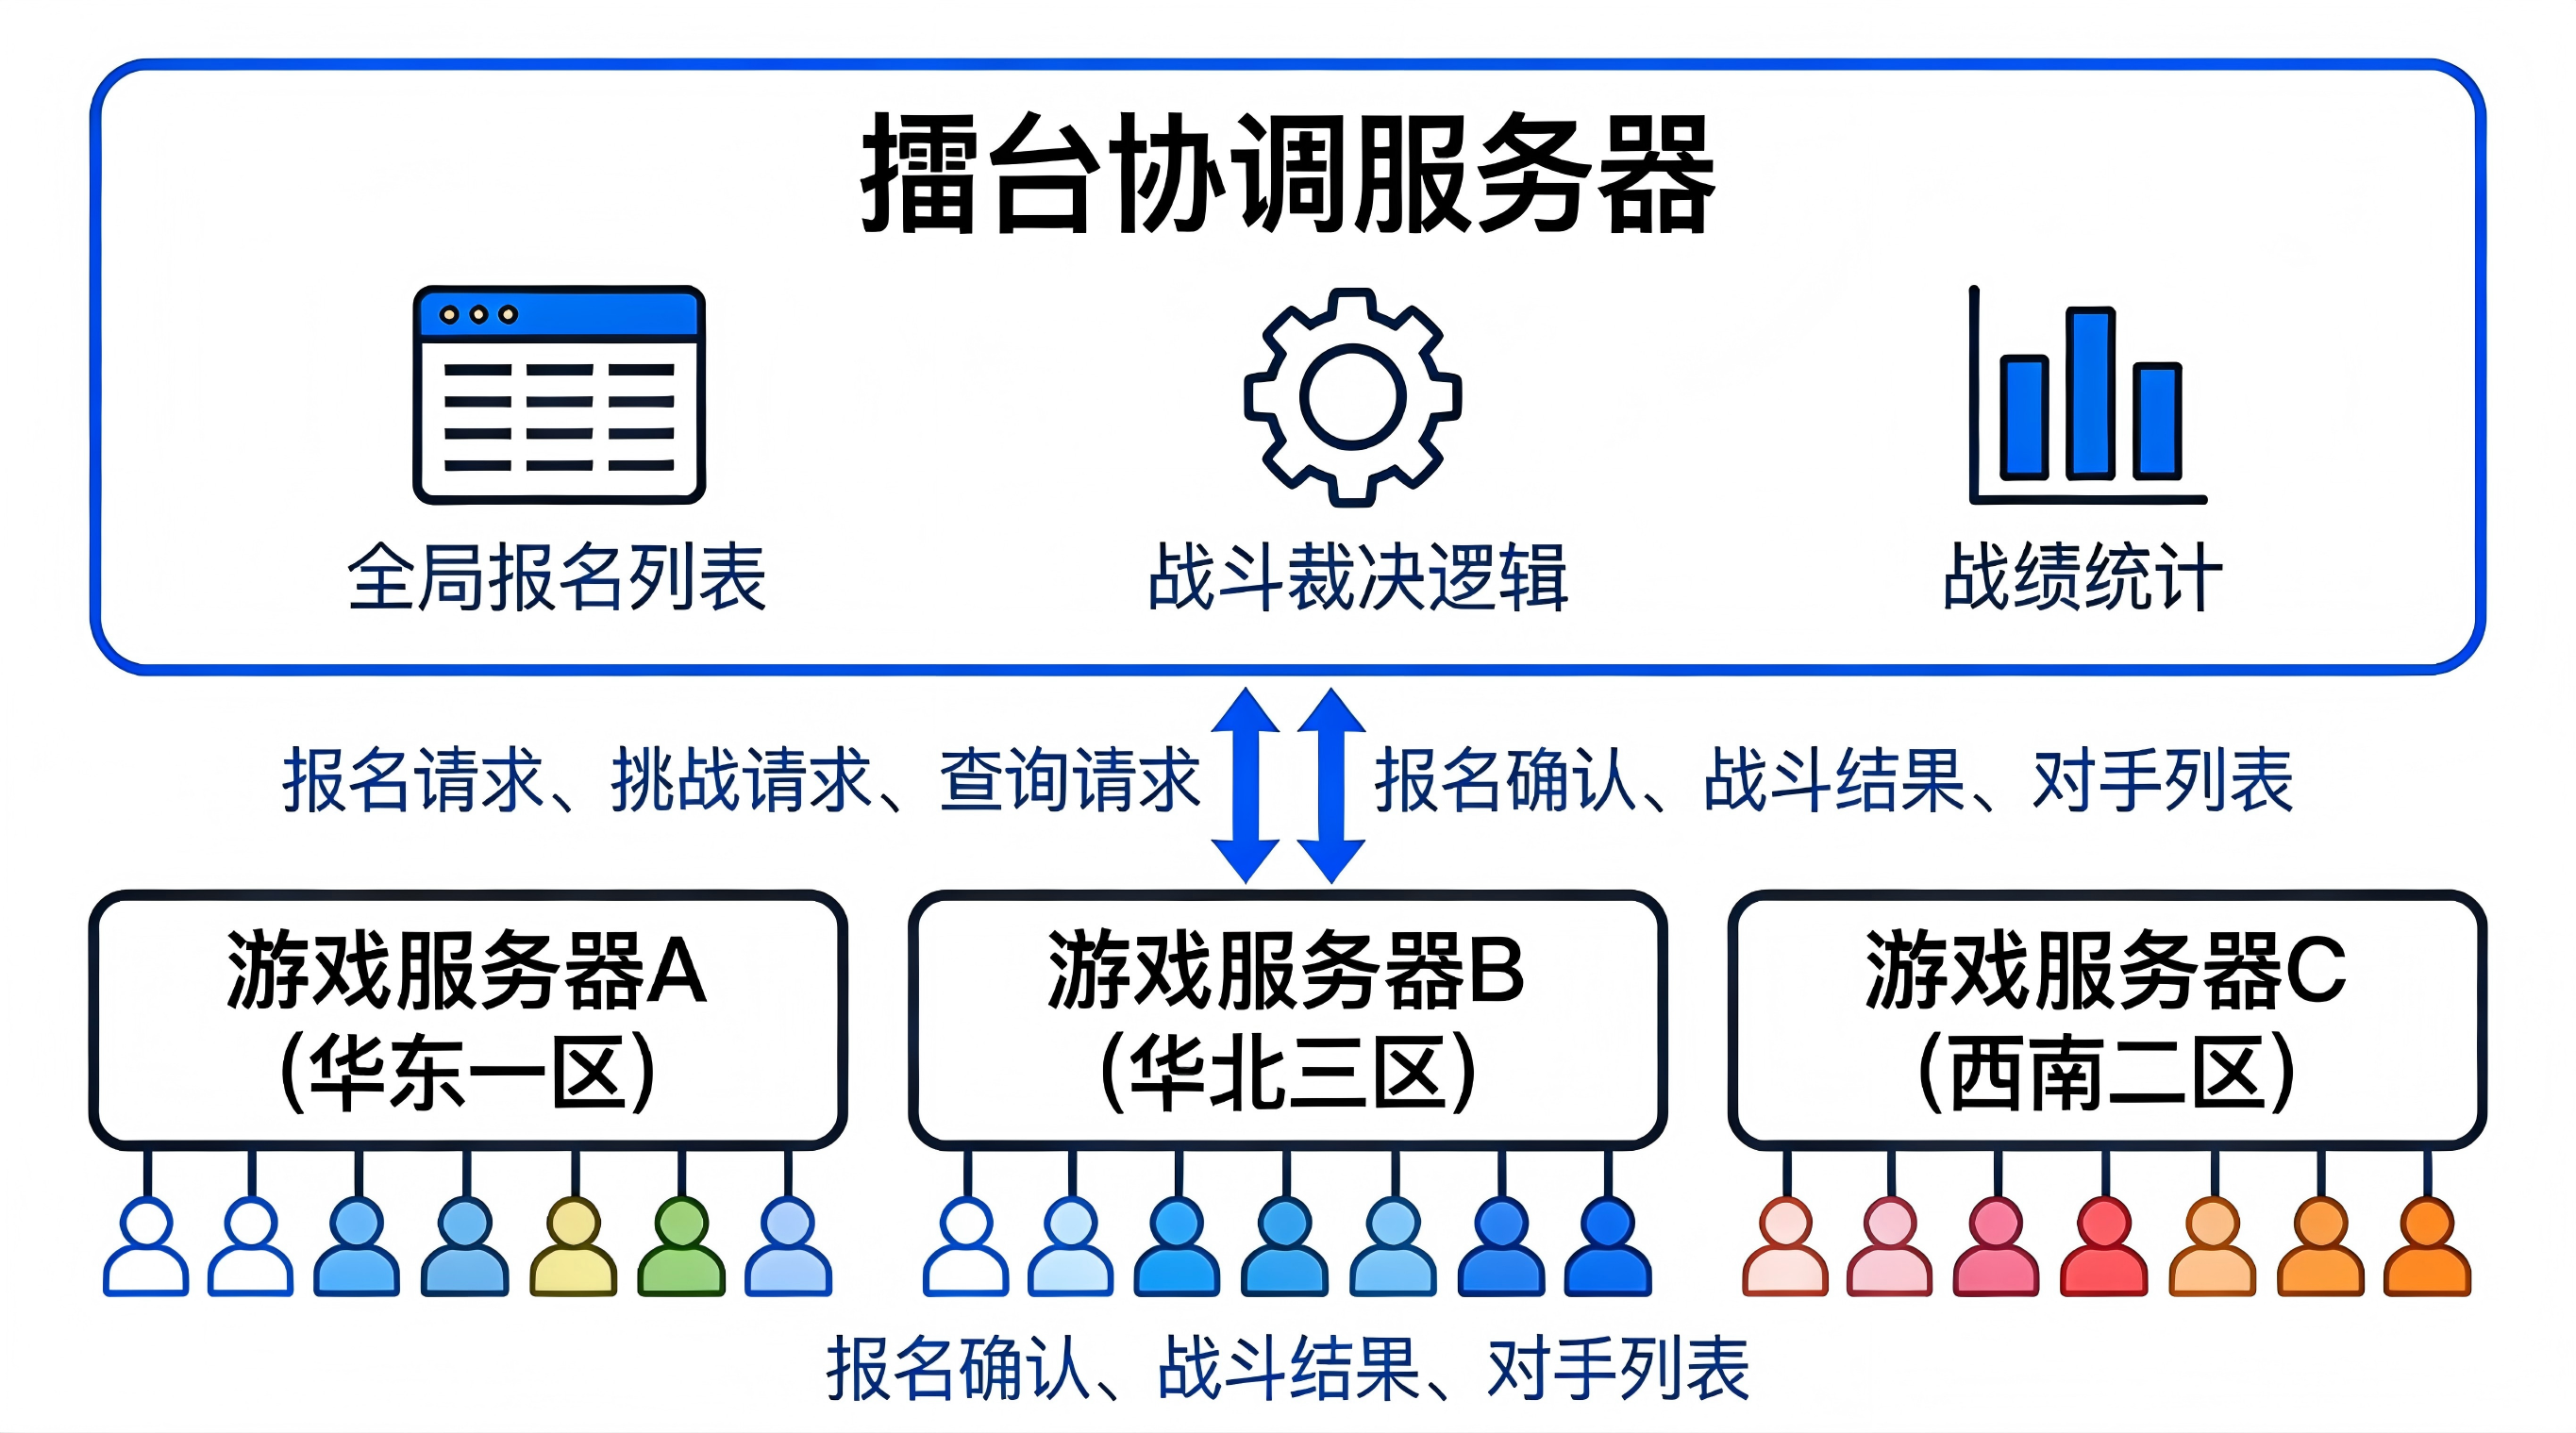
\includegraphics[width=1\linewidth]{figures/sec4/4-4.png}
    % 图片描述：跨服擂台的架构示意图
    % 顶部：一个大的矩形框，标注"擂台协调服务器"，内部包含：
    %   - "全局报名列表"（表格图标）
    %   - "战斗裁决逻辑"（齿轮图标）
    %   - "战绩统计"（柱状图图标）
    % 底部：三个游戏服务器并排，分别标注"游戏服务器A（华东一区）"、"游戏服务器B（华北三区）"、"游戏服务器C（西南二区）"
    % 每个游戏服务器下方连接若干玩家图标
    % 游戏服务器与擂台协调服务器之间有双向箭头，标注：
    %   - 上行箭头："报名请求、挑战请求、查询请求"
    %   - 下行箭头："报名确认、战斗结果、对手列表"
    % 用不同颜色区分不同服务器的玩家
    % 所有文字使用简体中文
    \caption{跨服擂台的整体架构}
    \label{fig:cross_server_arena_architecture}
\end{figure}

在这种架构下，擂台协调服务器承担了一个跨服视角下的"统一真相源"角色。它知道有哪些玩家正在参与擂台——无论这些玩家来自哪个服务器、数据存储在哪个分片——他们各自的战力是多少、目前是否在战斗之中、已经打了多少场、胜率如何。这一层信息在逻辑上属于全局，没有哪个单独的游戏服务器可以声称"我拥有全部擂台的信息"。即使是人数最多的服务器，也只知道本服玩家的情况，对其他服务器的玩家一无所知。而各个游戏服务器则负责把这一全局真相以本服玩家能够理解和感知的方式呈现出来：在界面上以列表展示所有参赛玩家，在本地记录本服玩家的胜负场次、更新积分和排名、发放奖励。从数据流的角度看，擂台协调服务器是"上游"，负责维护全局状态和做出权威裁决；各个游戏服务器是"下游"，负责接收上游的指令并在本地执行。这种单向的数据流和清晰的职责划分，是保证跨服系统正确运行的关键。

\subsubsection{报名与查询：全局状态的构建}

现在我们逐一分析跨服擂台的几个核心流程。首先是报名流程。当玩家小明在"华东一区"的游戏服务器上点击"报名参赛"按钮时，客户端会向游戏服务器发送一条报名请求消息。游戏服务器收到这条消息后，首先会执行一系列本地的前置检查：玩家等级是否达到参赛要求（比如至少 30 级）？玩家当前是否处于其他战斗中？玩家是否已经在擂台中报名？玩家今天是否还有剩余的报名次数？玩家的战力值是否已正确计算？这些检查的目的是在数据离开本服之前，就把明显不合法的请求过滤掉，减轻协调服务器的压力，也能更快地给玩家反馈。

如果所有检查都通过，游戏服务器会提取玩家的关键信息，构造一条报名请求，发送给擂台协调服务器。这条请求中包含玩家 ID、昵称、战力值、所属服务器 ID、报名时间戳等信息。擂台协调服务器收到报名请求后，也会执行一系列检查：检查这个玩家 ID 是否已经在全局的报名列表中（注意这里检查的是全局列表，即使玩家之前在另一台游戏服务器上报名，也能被检测到）；检查擂台当前是否已达到人数上限（为了保证系统性能和用户体验，擂台可能会设置一个参赛人数上限，比如最多 10 万人）；检查擂台当前是否处于开放时间（有些擂台玩法会设置固定的开放时间，比如每周六 14:00-16:00）；检查擂台是否正在维护。

\begin{tcolorbox}[title=报名请求的处理流程]
\begin{lstlisting}[
    language=go,
    basicstyle=\ttfamily\footnotesize,
    aboveskip=0pt, belowskip=0pt,
    lineskip=-1pt,
    commentstyle=\color{gray},
    keywordstyle=\color{blue}\bfseries,
    breaklines=true
]
// 游戏服务器：本地检查 -> 构造请求
if player.Level < 30 {
    return "等级不足，需要30级"
}
req = {PlayerID, Nickname, PowerValue, ServerID, Timestamp}
resp = arenaCoordinator.Register(req)

// 协调服务器：全局检查 -> 添加到列表
if alreadyExists(req.PlayerID) {
    return "已经报名"
}
addToGlobalList(req)
return {Success: true, TotalPlayers: len(globalList)}
\end{lstlisting}
\end{tcolorbox}

如果一切正常，协调服务器会将玩家信息添加到全局的报名列表中，并返回报名成功的响应。响应中包含当前的总参赛人数，游戏服务器收到后会在界面上显示"报名成功！当前全区共有 8327 名玩家参赛"，给玩家一个直观的反馈——这个数字不仅仅是本服的参赛人数，而是所有服务器加起来的总数，这正是跨服玩法的魅力所在。

报名成功后，玩家需要看到当前有哪些对手可以挑战。最直接的做法是，游戏服务器向擂台协调服务器发起一个查询请求："给我当前所有已报名且未在战斗中的玩家列表。"协调服务器遍历全局的报名列表，筛选出符合条件的玩家，将完整的列表返回给游戏服务器。但这种做法在擂台人数较多时会遇到性能问题。假设有 10 万玩家报名，每个玩家的信息包含 ID、昵称、战力值、服务器 ID 等字段，平均每条记录 100 字节，完整的列表就是 10MB 的数据。如果同时有 1000 个玩家在查询对手列表，协调服务器需要在短时间内发送 10GB 的数据，这对网络带宽和服务器 CPU 都是巨大的压力。更严重的是，这 10 万条记录中，大部分玩家对于当前请求的玩家来说都是"不相关"的——比如战力相差太大的玩家，挑战胜算很小或根本没有挑战价值。

因此，实际系统中通常会采用分页查询和条件筛选的方式。玩家不是一次性拿到所有对手的列表，而是先拿到一小部分（比如 50 个），在界面上滚动浏览时再加载更多。同时，查询请求中可以携带筛选条件，比如"只返回战力在我 ±5000 范围内的对手"、"只返回胜率低于 60\% 的对手"、"优先返回与我同服务器的对手"等，大大减少返回的数据量。协调服务器在收到查询请求后，会先根据筛选条件过滤出符合要求的玩家，再按战力值或其他维度排序，最后截取指定页码的数据返回。这样每次请求返回的数据量可以控制在一个合理的范围内（比如 50 条记录约 5KB），即使有数万玩家同时查询，协调服务器也能稳定应对。

\subsubsection{挑战与裁决：唯一真相源的必要性}

当玩家从对手列表中选择一个目标并点击"挑战"按钮时，整个系统进入了最核心的环节：战斗裁决。游戏服务器会构造一条挑战请求，包含挑战者的玩家 ID 和被挑战者的玩家 ID，发送给擂台协调服务器。协调服务器收到挑战请求后，首先要做一系列的合法性检查，这是保证系统正确性和公平性的关键：挑战者和被挑战者是否都在报名列表中（有可能某个玩家刚刚取消报名或被系统移除，但客户端界面还没刷新）？挑战者和被挑战者是否都处于"空闲"状态（如果其中任何一方正在进行其他战斗，不允许开始新的战斗，避免一个玩家同时参与多场战斗导致状态混乱）？挑战者今天的挑战次数是否已用完？挑战者是否在冷却时间内？

如果所有检查都通过，协调服务器会将双方的状态标记为"战斗中"，防止在战斗结束之前被其他玩家同时挑战。想象一下，如果玩家 A 正在与玩家 B 战斗，此时玩家 C 也向 B 发起挑战，那 B 应该同时与 A 和 C 战斗吗？显然不合理。通过状态锁定机制，我们确保同一时刻一个玩家只能参与一场战斗。

接下来是战斗裁决的核心逻辑。在我们简化的跨服擂台中，战斗规则非常简单：比较双方的战力值，战力值更高的一方获胜。如果战力值相等，可以引入随机因素或其他平局打破器（比如等级、装备品质）。协调服务器执行裁决后，会生成一个战斗结果事件，记录胜者和败者，并更新双方的擂台战绩——比如胜者的胜场数加一，败者的负场数加一。战斗结算完成后，协调服务器会将双方的战斗状态恢复为"非战斗中"，并将战斗结果事件分别发送给挑战者和被挑战者所属的游戏服务器。

\begin{tcolorbox}[title=战斗裁决的核心流程]
\begin{lstlisting}[
    language=go,
    basicstyle=\ttfamily\footnotesize,
    aboveskip=0pt, belowskip=0pt,
    lineskip=-1pt,
    commentstyle=\color{gray},
    keywordstyle=\color{blue}\bfseries,
    breaklines=true
]
// 1. 锁定双方状态
challenger.Status = "fighting"
defender.Status = "fighting"

// 2. 战斗裁决（简化规则：战力高者胜）
if challenger.Power > defender.Power {
    winner = challenger
} else {
    winner = defender
}

// 3. 更新战绩并解锁状态
winner.Wins++, loser.Losses++
challenger.Status = "idle", defender.Status = "idle"

// 4. 分发结果到双方服务器
sendResult(challengerServer, result)
sendResult(defenderServer, result)
\end{lstlisting}
\end{tcolorbox}

注意这里是"分别发送"——挑战者可能在服务器 A，被挑战者可能在服务器 B，协调服务器需要向两台不同的服务器各发送一条消息，通知它们战斗的结果。各个游戏服务器收到战斗结果事件后，需要根据事件中的信息更新本地玩家的数据。如果本服玩家是胜者，游戏服务器会增加玩家的擂台积分、发放胜利奖励（比如金币、擂台代币）、更新任务进度（比如"赢得 10 场擂台战斗"）；如果本服玩家是败者，则可能扣除一些积分或记录失败次数。这些更新操作完全在本地进行，不需要再与擂台协调服务器或其他服务器通信，从而避免了复杂的分布式事务。

需要强调的是，各个游戏服务器在收到战斗结果事件后，并不会对结果本身进行任何质疑或修改。它们只是忠实地执行擂台协调服务器给出的裁决，将结果体现在本地数据和界面表现中。即使某个游戏服务器的本地数据显示玩家的战力已经发生了变化（比如玩家在战斗开始后、结果返回前换了一件更好的装备），也不会重新计算战斗结果，因为战斗裁决是基于挑战发起时的战力值，而不是结果返回时的战力值。这种"单点裁决、多点跟随"的模式，确保了跨服擂台的战斗结果在所有相关服务器上保持一致，避免了"双重历史"的问题。

所谓"双重历史"，指的是不同服务器对同一个事件有不同的记录和理解。如果我们允许每一台游戏服务器各自独立地为本服玩家做出裁决，就有可能出现这样的矛盾场景：挑战者小明在服务器 A，被挑战者李四在服务器 B。小明发起挑战，服务器 A 读取本地的玩家数据，计算出小明的战力是 32000；同时，服务器 B 读取李四的数据，计算出李四的战力是 31000。如果服务器 A 和服务器 B 各自独立裁决，都会判定本服玩家获胜（服务器 A 认为小明 32000 > 李四 31000，服务器 B 可能因为数据同步延迟，还没收到小明最新的战力值，认为李四 31000 > 小明 30000）。最终的结果是：小明的战绩增加了一场胜利，李四的战绩也增加了一场胜利，两个人都认为自己赢了，但实际上只有一场战斗发生。这种"双重历史"不仅会导致数据不一致，还会严重破坏玩家对游戏公平性的信任——当两个玩家线下交流时，发现同一场战斗有两个完全相反的结果，他们会怎么想？

% 为了避免这种问题，跨服擂台引入了一个逻辑上唯一的裁决点——擂台协调服务器。所有挑战请求，无论起点在哪一台游戏服务器上，最终都在这个协调服务器上汇聚。协调服务器维护着一份权威的、全局的玩家信息表，记录每个玩家最新的战力值、战斗状态、战绩统计。当收到挑战请求时，协调服务器从这个全局表中读取双方的战力值，执行裁决逻辑，得出唯一的、权威的战斗结果。然后，这个结果以事件的形式被分发给相关的游戏服务器，各服务器只负责执行，不负责裁决。

为了避免这种问题，跨服擂台引入了一个逻辑上唯一的裁决点——擂台协调服务器。
所有挑战请求，无论起点在哪一台游戏服务器上，最终都在这个协调服务器上汇聚。
协调服务器维护着一份权威的、全局的玩家信息表，记录每个玩家最新的战力值、
战斗状态、战绩统计。当收到挑战请求时，协调服务器从这份全局表中读取双方的战力值，
执行裁决逻辑，得出唯一的、权威的战斗结果。

然而，在将结果向外分发之前，有一个容易被忽视但至关重要的一致性问题必须在这一步解决：
"小明胜"和"李四负"这两条消息，必须作为一个不可分割的原子单元同时写入，
而不能先写一条再写另一条。如果只保证"写入成功的消息最终会被处理"，
却没有保证"两条消息一定同时写入成功"，那么一旦协调服务器在写入第一条之后、
写入第二条之前崩溃，就会出现消息队列里只有赢家没有输家的情况——
后续无论重试多少次，也只会一遍又一遍地处理那条已经写入的赢家消息，
而输家的战绩永远不会更新。这与单机数据库中"部分成功"的事务问题本质相同，
只是发生的位置从数据库层面移到了消息写入层面。

解决这一问题的关键在于：协调服务器完全不需要引入跨节点的两阶段提交（2PC），
因为这里的所有写入操作都发生在同一个地方——协调服务器自己的本地数据库上。
协调服务器只需用一个普通的本地 ACID 事务，将三件事打包成一个原子操作：
记录对战结果（一输一赢写入 \texttt{match\_results} 表）、
同时向发件箱表（\texttt{outbox}）中写入两条待发消息——一条给服务器 A，
一条给服务器 B。这个事务要么整体提交（对战记录和两条待发消息全部落盘），
要么整体回滚（什么都不写，双方均未收到任何通知，状态完全一致）。
由于三行写入都在同一个数据库实例上，普通的本地事务就足以保证原子性，
无需任何跨节点协调协议。

事务提交之后，一个后台的发件箱派发程序（Outbox Dispatcher）持续轮询
\texttt{outbox} 表，将其中尚未投递的消息异步地发送给对应的游戏服务器。
每条消息都携带一个唯一的 \texttt{match\_id} 作为幂等键，
游戏服务器在处理消息时先检查该 \texttt{match\_id} 是否已经处理过，
若已处理则直接忽略，从而避免重复执行。若某次投递因网络抖动失败，
发件箱记录不会被删除，Dispatcher 在下一轮轮询时会自动重试，
直到成功为止。这种"事务性发件箱 + 幂等重试"的模式，
保证了两条消息在事务层面"同生同死"，又在传输层面"最终一定送达"，
兼顾了原子性和可用性。完整的流程如图~\ref{fig:cross_server_challenge_flow} 所示。

需要强调的是，这套方案与前文所讨论的两阶段提交在解决问题的层次上是不同的。
2PC 用于协调\textbf{多个独立数据库节点}之间的跨节点事务，
其高昂代价来自于跨网络的锁定和协调。而这里的原子写入发生在协调服务器
\textbf{单个本地数据库}内部，本地 ACID 事务完全胜任，根本不需要 2PC。
各个游戏服务器更新本地战绩、积分、奖励的操作，
则被显式地降级为"允许延迟、保证最终一致"的异步处理——
玩家体验上，战绩几秒后才刷新完全可以接受，
这远比因引入 2PC 而导致整个战斗结算流程被锁定等待要好得多。

\begin{figure}[htbp]
    \centering
    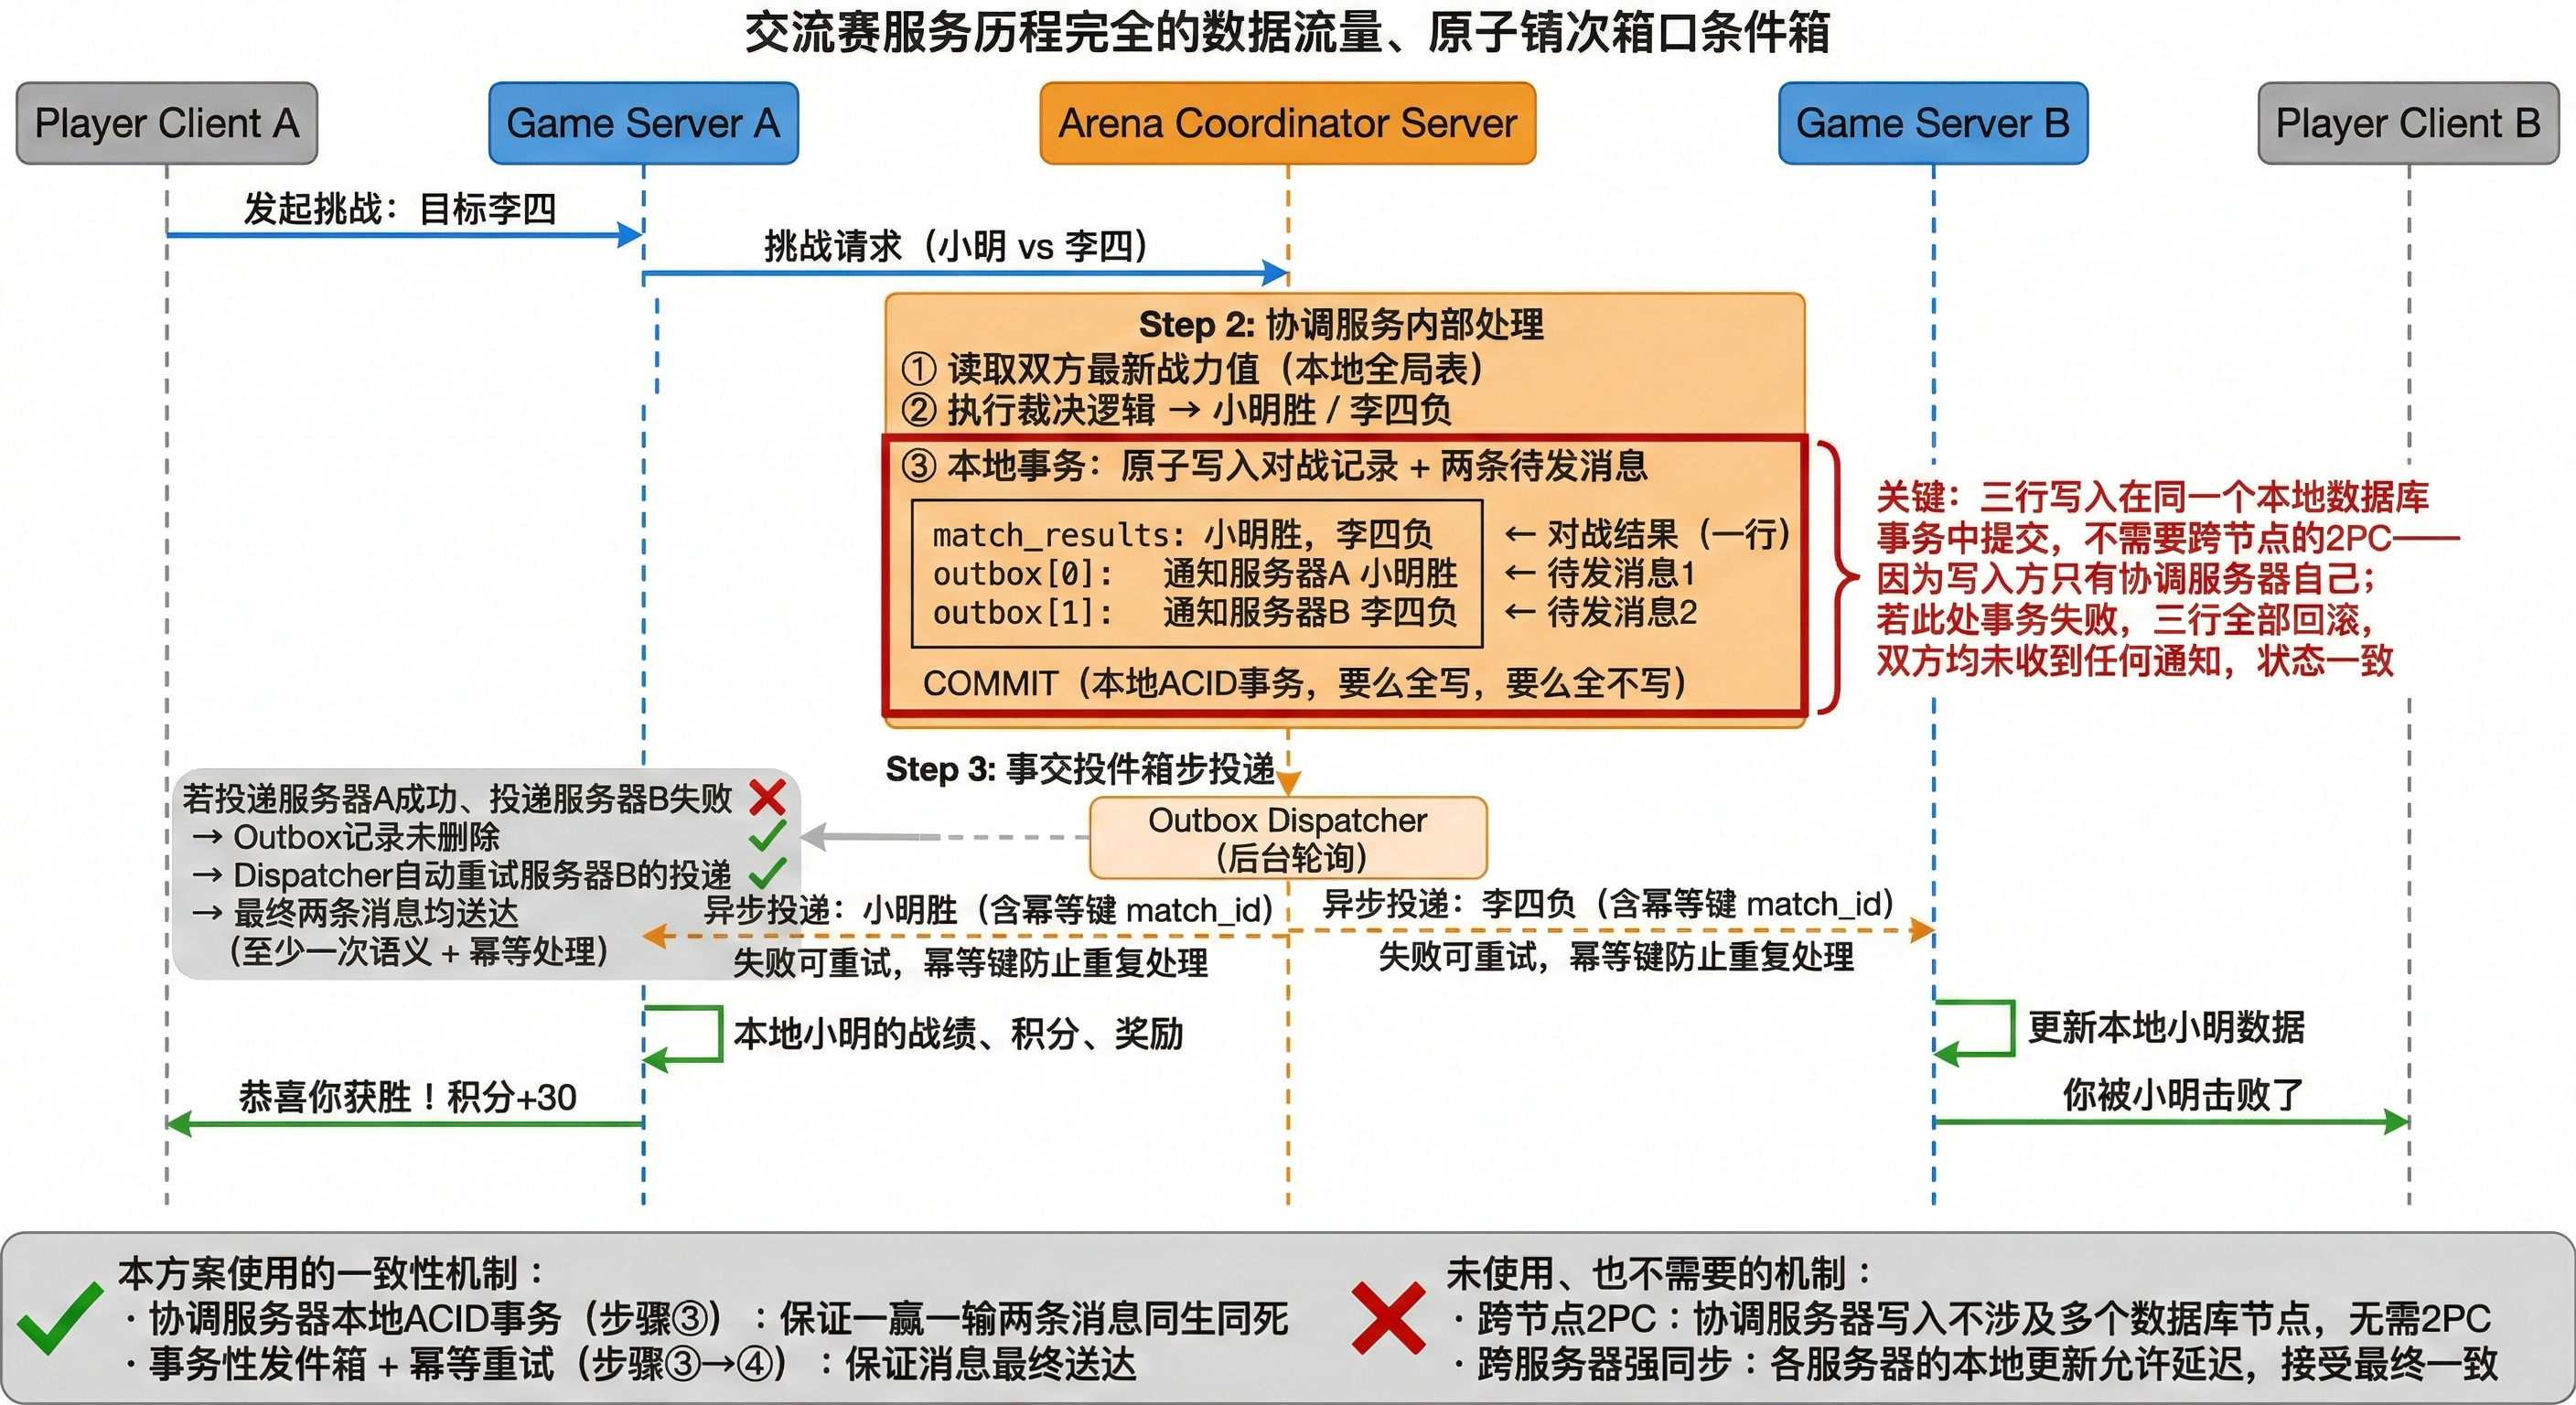
\includegraphics[width=1\linewidth]{figures/sec4/4-5.png}
    \caption{跨服擂台完整数据流：协调服务器以单个本地事务原子写入对战结果与两条待发消息，
    事务性发件箱保证两条消息同生同死，后台 Dispatcher 以幂等重试确保最终送达；
    各游戏服务器的本地战绩更新允许异步延迟，无需跨节点 2PC}
    \label{fig:cross_server_challenge_flow}
\end{figure}


\subsubsection{容错与高可用：协调服务器的挑战}

引入单点裁决解决了一致性问题，但也随之带来了一个新的挑战：
如果擂台协调服务器崩溃了怎么办？
它是整个跨服擂台系统的核心裁决点，一旦宕机，
所有服务器的玩家都无法发起挑战、查询排名、提交报名，整个玩法立刻瘫痪。
因此，协调服务器不能以单台机器的形式存在，
而必须被扩展为一个多节点的高可用集群。
图~\ref{fig:coordinator_cluster_arch} 展示了这个集群在整个跨服擂台系统中的位置：
游戏服务器将所有挑战请求发往集群中当前的 Leader 节点，
Leader 负责裁决并将结果持久化到下方的数据库，
同时通过事务性发件箱将结果异步派发回各游戏服务器；
集群内部的多个节点之间持续同步数据，使得任意一个节点崩溃后，
其他节点都能立刻接管服务。

\begin{figure}[htbp]
    \centering
    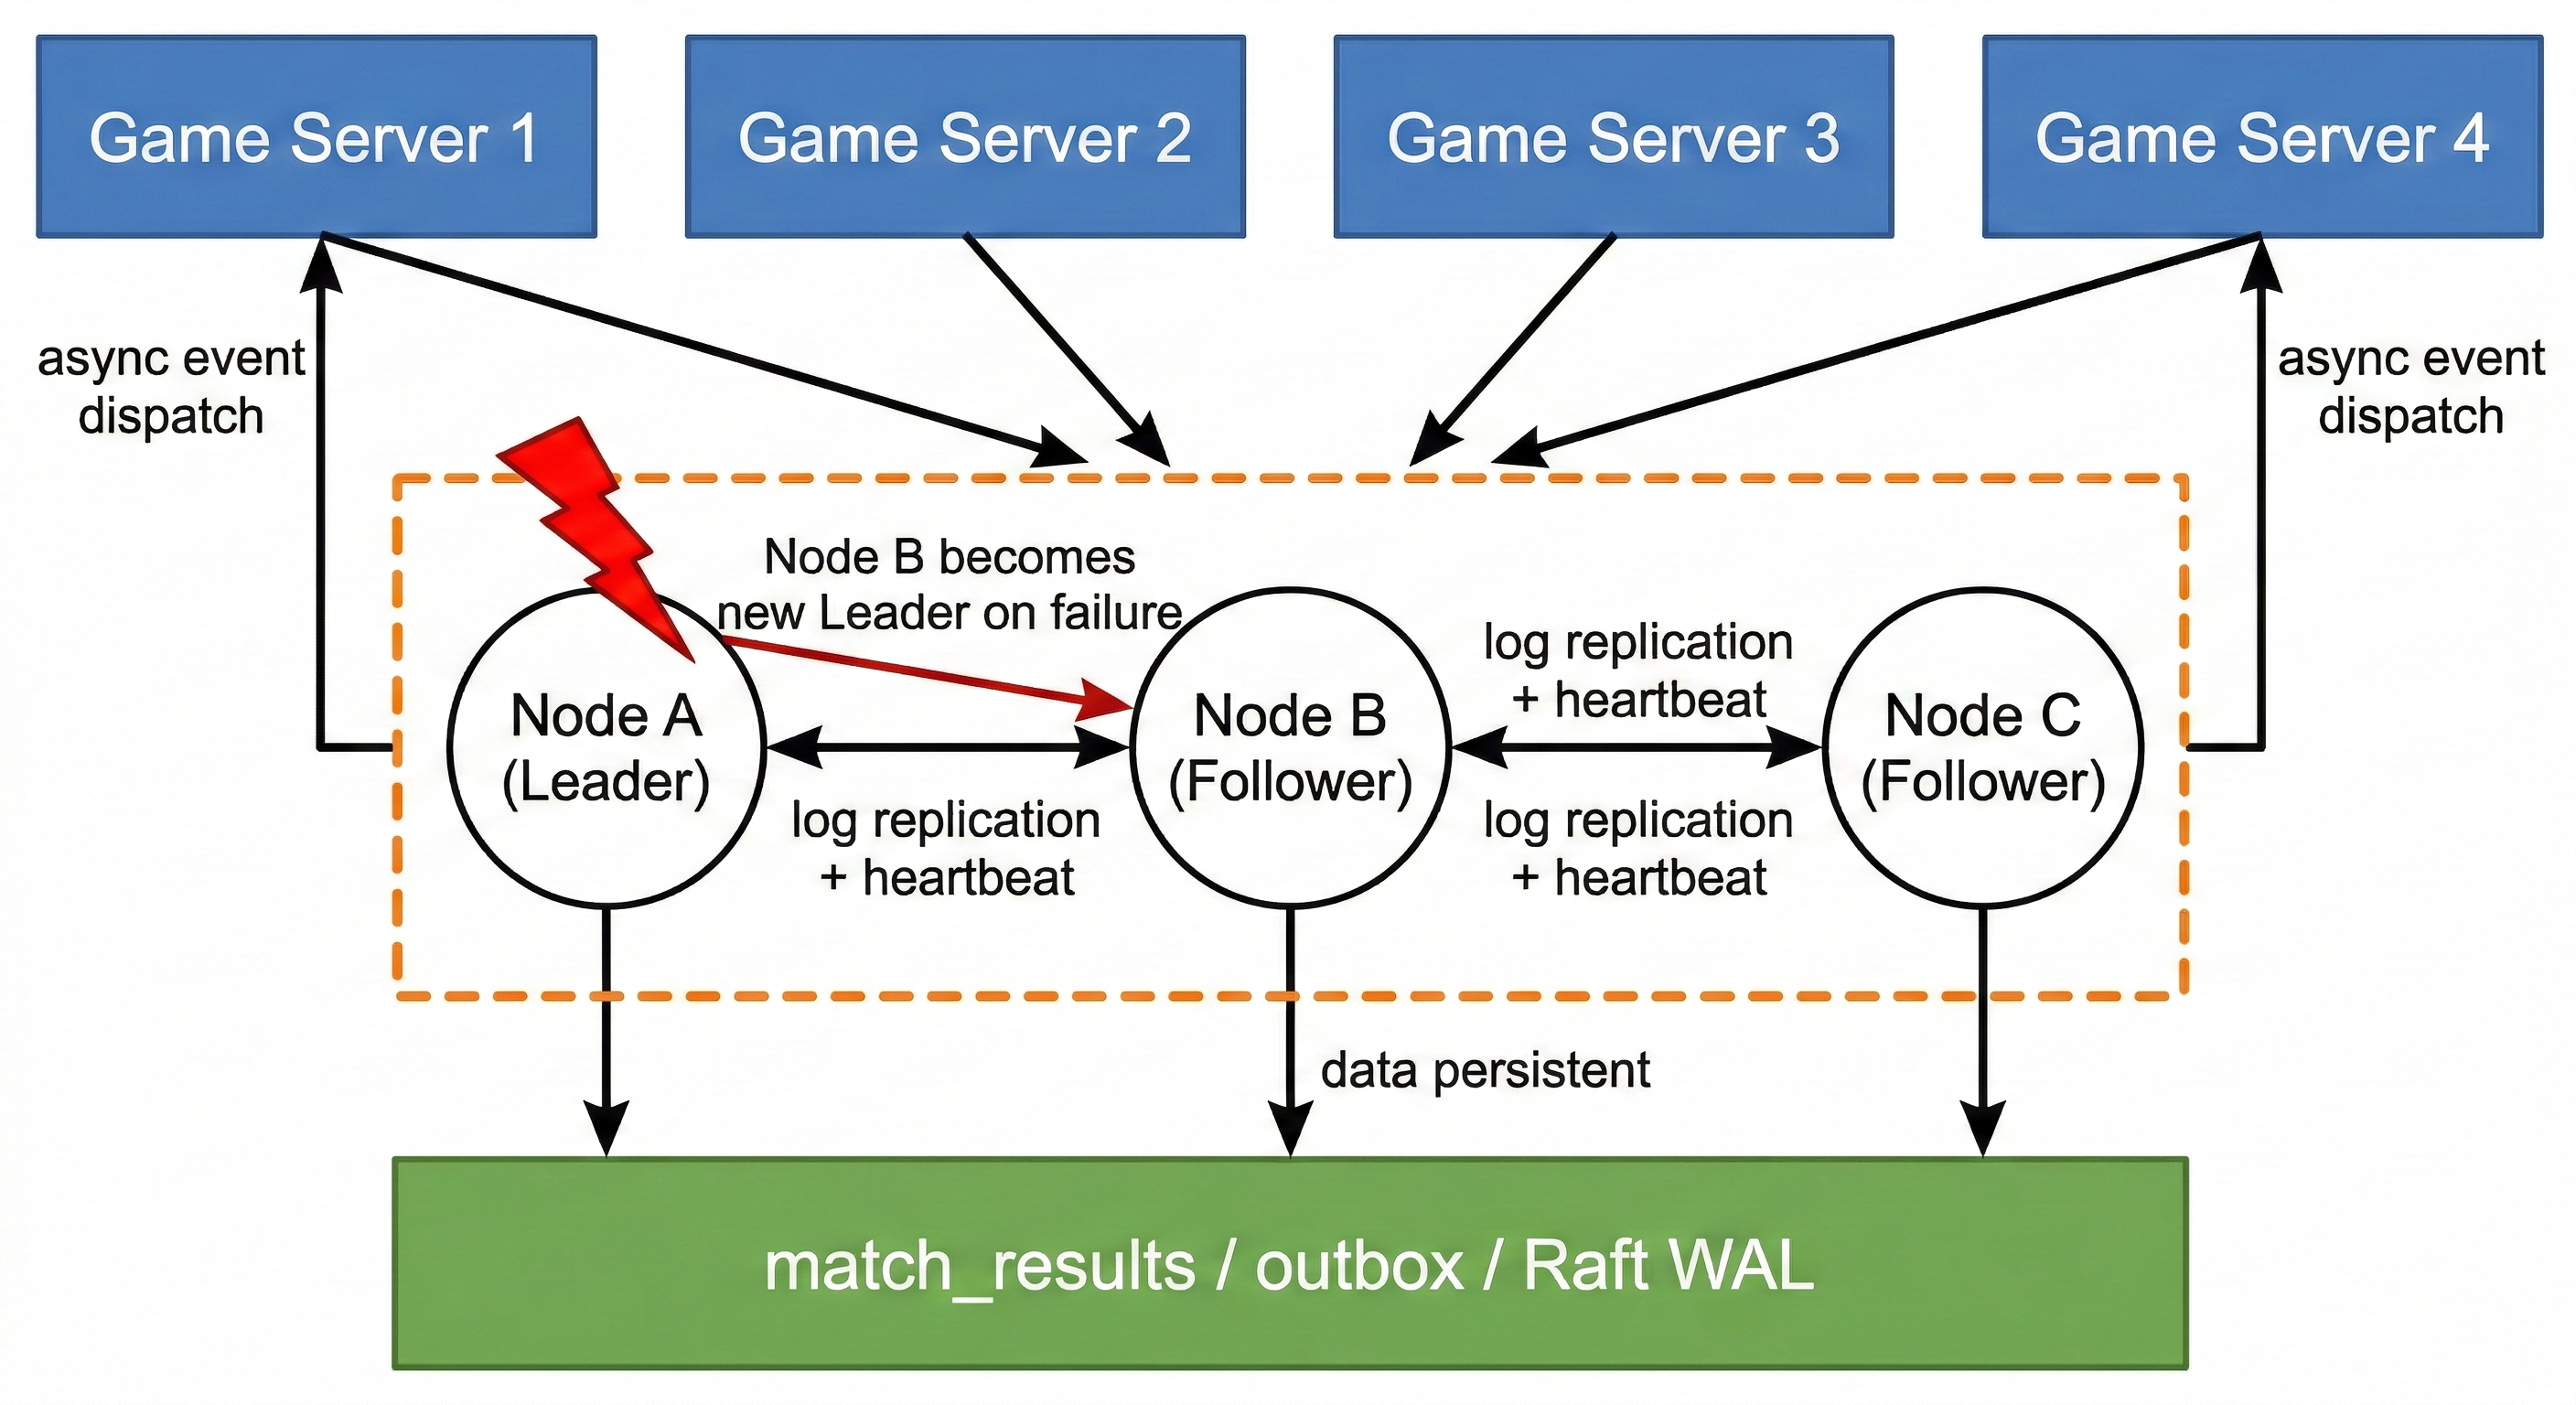
\includegraphics[width=1\linewidth]{figures/sec4/4-coord-arch.png}
    \caption{跨服擂台系统架构：游戏服务器将请求发往协调服务器集群的 Leader，
    集群通过 Raft 协议维护多节点一致性，Leader 崩溃后集群自动选出新 Leader}
    \label{fig:coordinator_cluster_arch}
\end{figure}

构建多节点集群，首先面对的是一个基本问题：集群里谁说了算，以及如何让所有节点
对"操作历史"始终保持一致的认知？这正是分布式系统中经典的共识（Consensus）问题。
Raft 算法由 Diego Ongaro 和 John Ousterhout 于 2014 年提出，
其核心设计目标便是"可理解性"——将共识问题显式地拆解为领导者选举、
日志复制和安全性约束三个子问题分别处理，使得工程师能够清楚地推理系统在各种故障下的行为。

\paragraph{节点角色与任期}

Raft 将集群中的每个节点建模为一个状态机，节点在任意时刻处于三种角色之一：
跟随者（Follower）、候选者（Candidate）或领导者（Leader）。
集群正常运行时只存在一个 Leader，它是唯一接受外部写请求的权威节点；
其余节点均为 Follower，被动接收来自 Leader 的日志和心跳。
Raft 使用单调递增的整数"任期"（Term）来标识时间区段，
每个任期最多只有一个合法的 Leader——这一"任期唯一性"是 Raft
所有安全性保证的出发点。

\paragraph{领导者选举}

每个 Follower 都维护一个随机化的选举超时计时器（通常在 150\,ms 到 300\,ms 之间随机取值）。
若在超时时间内未收到来自 Leader 的心跳，节点就认为当前没有合法的 Leader，
于是将自身切换为 Candidate，将 Term 加一，投票给自己，
并向所有其他节点发送 \texttt{RequestVote} 消息。
其他节点收到投票请求时，须同时满足两个条件才会投赞成票：
候选者的 Term 不小于自身当前的 Term，以及候选者的日志至少和自己一样新
（先比较最后一条日志的任期号，再比较其索引，取较大者为"更新"）。
每个节点在同一 Term 内只能投票给一个候选者。
某个候选者一旦收到超过半数节点的赞成票，即成为新 Leader，
立即向所有节点发送心跳，阻止其他节点再次发起选举。

随机化超时是防止"分票"（Split Vote）僵局的关键。
若所有节点同时超时并发起选举，每人只投自己，无人获得多数票，选举失败需重试。
随机化使得某一个节点几乎总是比其他节点提前超时，
率先收集到足够的选票，在其他节点触发超时之前就完成当选。
图~\ref{fig:raft_core} 左侧展示了一次完整的选举流程：
节点 A 率先超时当选（Term=2），随后 A 崩溃，节点 B 率先超时，
在 Term=3 中收集到 C 的投票后成为新 Leader，
总服务中断时间约等于一次选举超时长度。

\paragraph{日志复制}

Leader 选出之后，外部的每一个写请求都经由以下流程被持久化并执行，
如图~\ref{fig:raft_core} 右侧所示。以"小明挑战李四"为例：
Leader 收到请求后，先将其封装为带有索引和任期号的日志条目追加到本地日志，
此时该条目尚未提交（灰色）；随后 Leader 并发地将该条目通过
\texttt{AppendEntries} 消息复制到所有 Follower。
Follower 收到后先做"前缀匹配检查"——验证消息中携带的前一条日志的索引与任期
是否与自身日志末尾完全吻合，若不吻合则拒绝，Leader 会自动回退重试直到找到对齐点；
检查通过后 Follower 追加条目并回复成功。
当 Leader 收到超过半数节点（含自身）的成功回复后，
该条目被标记为"已提交"（Committed，绿色），
Leader 将其应用到状态机——在擂台场景中即执行裁决逻辑、
以本地 ACID 事务原子写入 \texttt{match\_results} 和 \texttt{outbox}。
此后 Leader 将 \texttt{commitIndex} 通过后续心跳告知所有 Follower，
Follower 也将该条目应用到本地状态机，三个节点最终持有完全相同的日志和状态。

提交只要求多数节点确认而非全部节点，这正是 Raft
能够在节点部分失联时仍然正常工作的根本原因：
三节点集群在一个 Follower 暂时失联时依然可以提交，
失联节点恢复后会自动通过日志同步补全缺失的条目。

\begin{figure}[htbp]
    \centering
    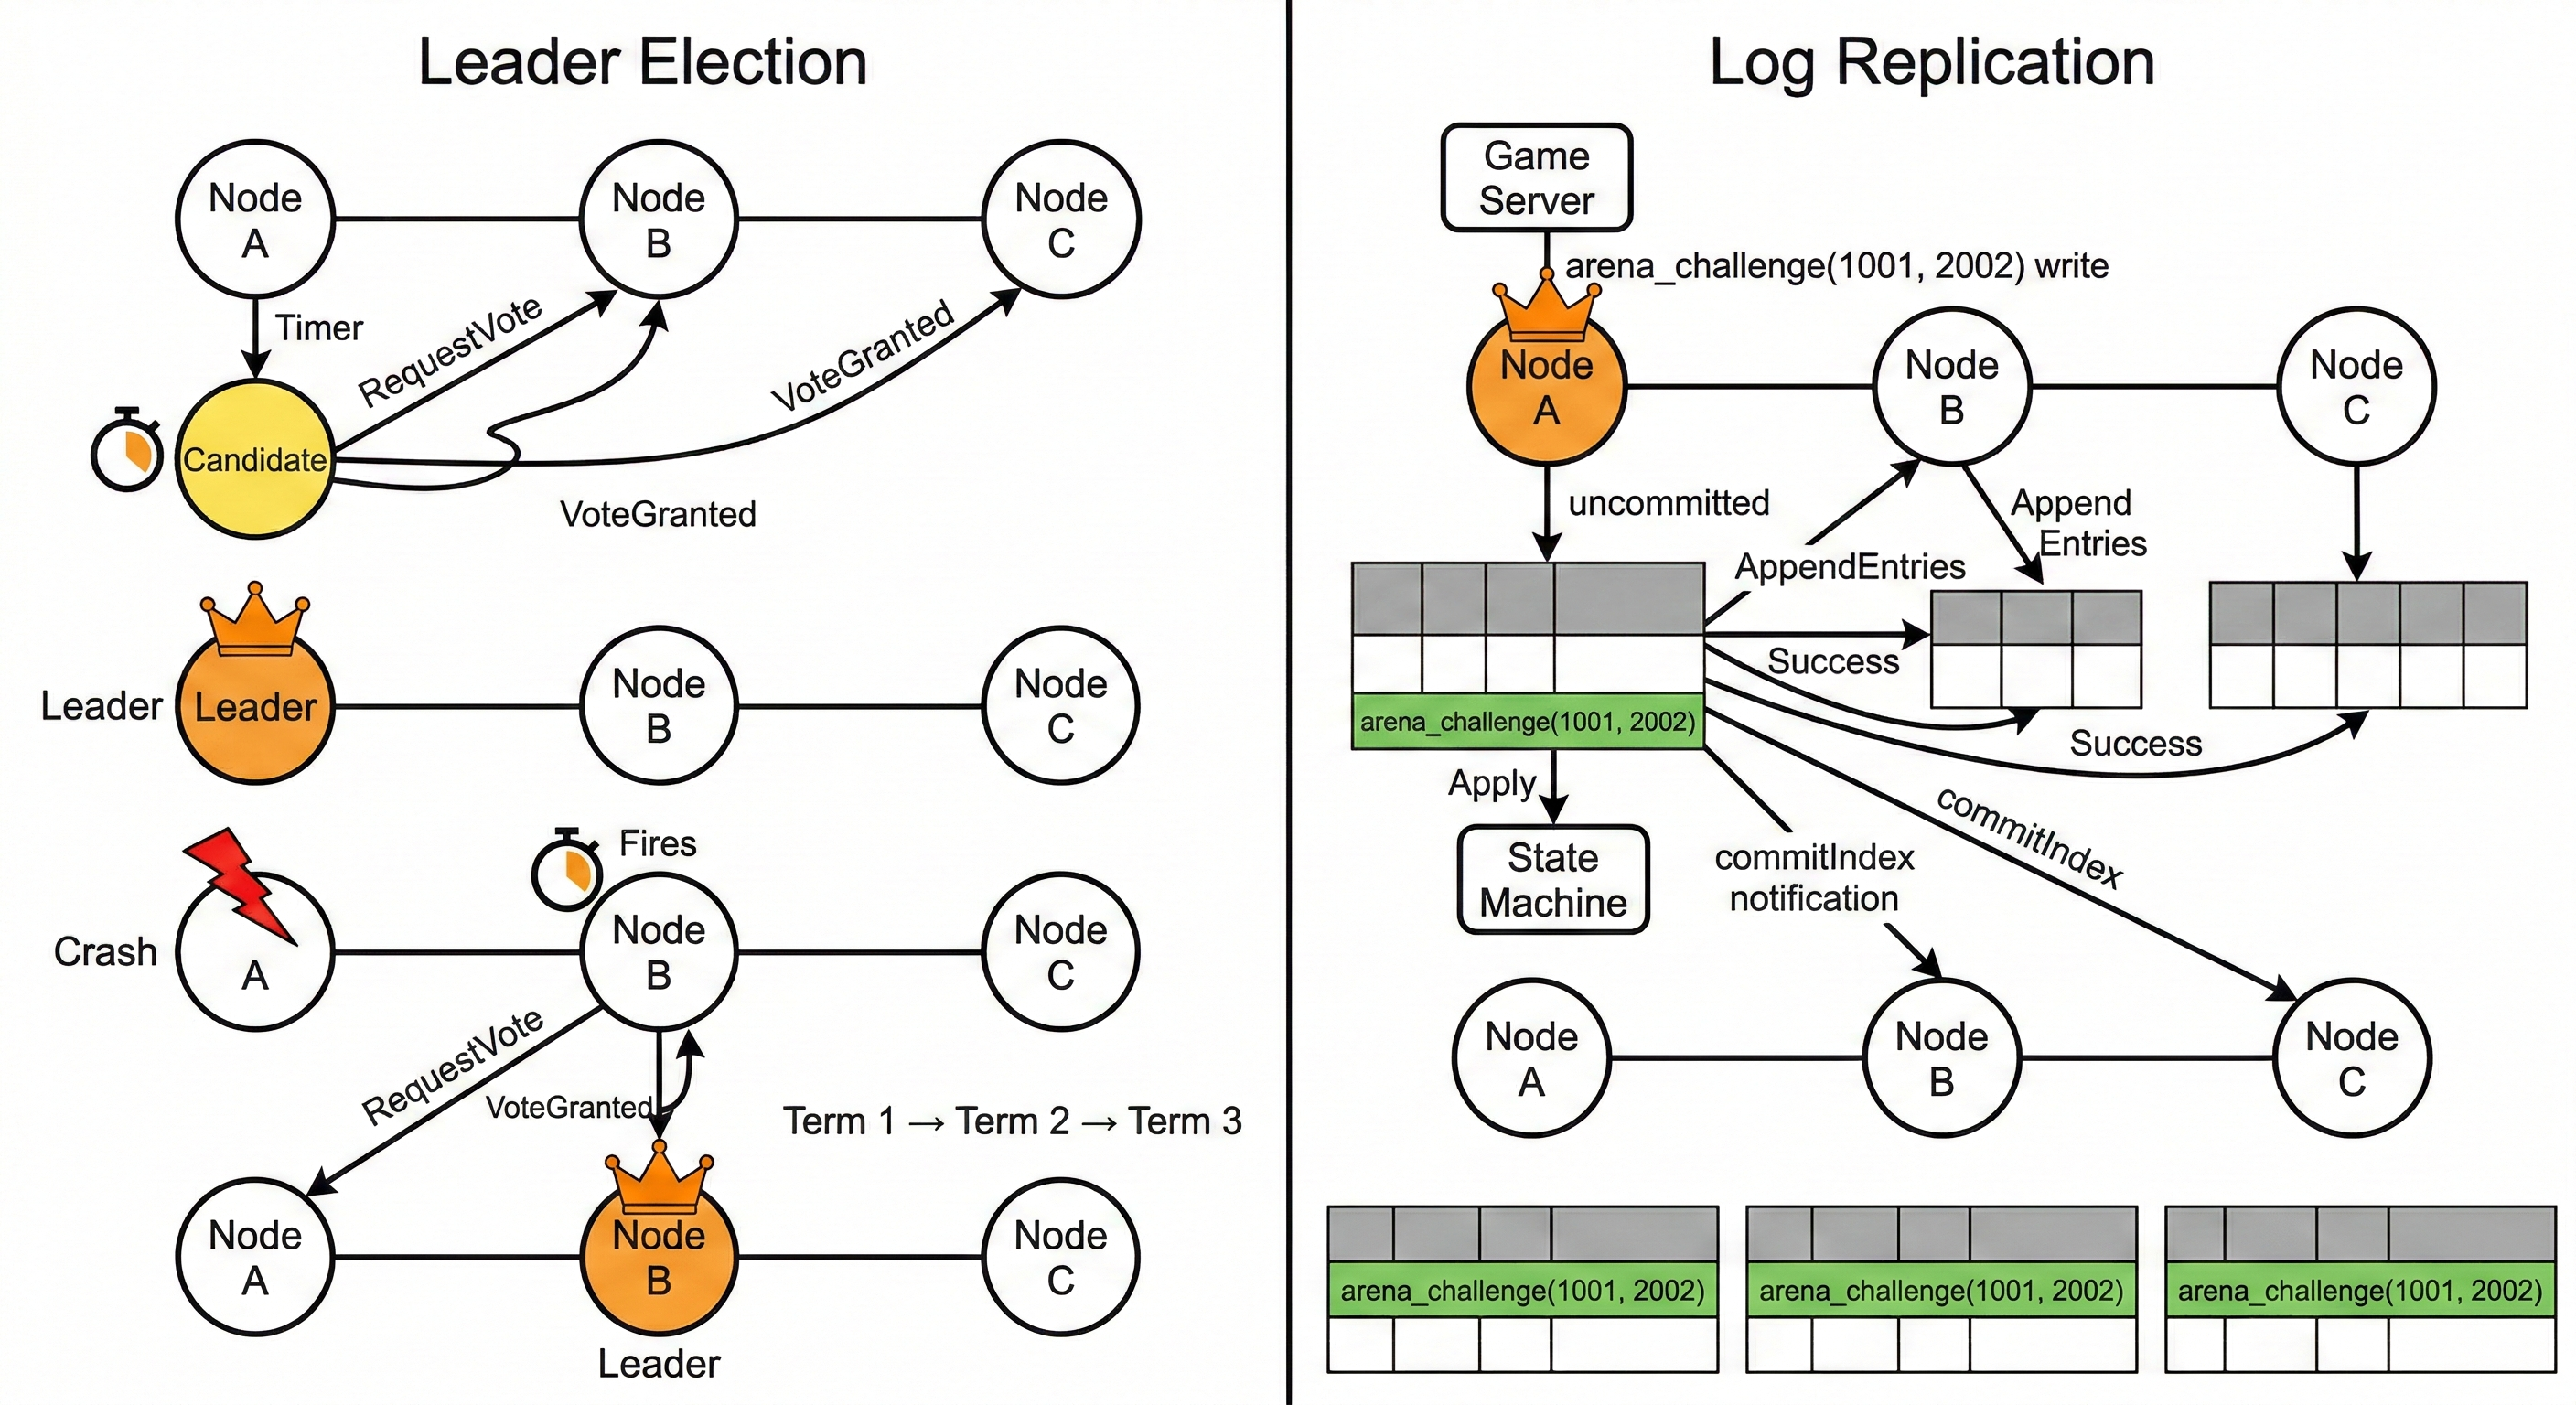
\includegraphics[width=1\linewidth]{figures/sec4/4-raft-core.png}
    \caption{Raft 核心机制（左）领导者选举：随机化超时防止分票，
    Term 单调递增保证不会选出过期节点；
    （右）日志复制：Leader 追加并复制日志，多数确认后提交，
    所有节点状态机最终一致}
    \label{fig:raft_core}
\end{figure}

\paragraph{安全性：为什么已提交的数据不会丢失}

Raft 最核心的安全性保证是：任何已提交的日志条目，
在集群经历任意节点崩溃和重新选举之后，都不会被覆盖或丢失。
这一保证来自选举时"日志最新"的约束。
一条日志条目被提交，意味着它已经存在于集群中超过半数的节点上；
而任何候选者想要当选，也必须获得超过半数节点的投票。
这两个"超过半数"的集合必然存在交集——至少有一个节点同时拥有已提交的条目
且参与了本次投票。该节点只会把票投给"日志至少和自己一样新"的候选者，
这就保证了新 Leader 的日志必然包含所有已提交的条目，
历史数据永不倒退。

\paragraph{集群规模与工程实践}

在实际部署中，协调服务器集群通常选择三节点或五节点配置。
三节点集群可容忍一台服务器同时故障（$\lfloor 3/2 \rfloor = 1$），
适合单机房的普通可用性场景；
五节点集群可容忍两台同时故障（$\lfloor 5/2 \rfloor = 2$），
适合需要跨机房部署或对可用性要求更高的场景。
Raft 日志本身就是持久化的载体：每个节点以 WAL（Write-Ahead Log）的形式
将日志顺序追加写入本地磁盘，崩溃重启后直接回放日志即可恢复状态。
当日志积累过长时，Raft 还支持快照压缩（Snapshotting）：
将当前完整的状态机快照落盘，删除快照之前的全部日志，
防止日志文件无限增长，同时保证新节点加入时能够快速同步状态。


\subsubsection{从简化到扩展：跨服擂台的演进空间}

通过这个完整的跨服擂台案例，我们看到了分布式架构的两个重要价值。第一，它不仅仅是为了"扛住更多人"，还能够支撑单机时代难以实现的玩法创新——只有当玩家被分散到多个服务器上，"跨服"这一概念才有存在的意义，而跨服玩法可以打破服务器壁垒，让所有玩家在一个更大的舞台上竞技，提升游戏的社交性和竞技性。第二，通过刻意简化战斗规则（只比较战力值，不模拟复杂战斗），这个案例让我们能够集中精力理解"协调服务器"、"唯一裁决"、"多服同步"等分布式系统的核心概念。

但简化并不意味着这个架构只能支撑简单的玩法。当我们理解了简化版本的跨服擂台如何工作之后，就可以逐步引入更复杂的战斗机制。例如，可以将战力比拼升级为回合制战斗：协调服务器不再只是比较一个数值，而是模拟多个回合的攻击与防御，每个回合根据双方的攻击力、防御力、技能效果计算伤害，直到某一方血量归零。这种扩展不需要改变整体架构——协调服务器仍然是唯一的裁决点，游戏服务器仍然是代理和执行者，只是裁决逻辑从简单的数值比较变成了多回合的战斗模拟。

进一步地，还可以引入技能释放和战术选择。玩家在挑战时不仅选择对手，还可以选择使用哪些技能、采用什么战术。协调服务器在裁决时会考虑这些因素，比如某个技能对某种类型的敌人有额外伤害，某个战术在先手时更有优势。这时协调服务器的裁决逻辑会更复杂，但核心的架构模式仍然不变——唯一真相源、单点裁决、多点跟随。

甚至可以探索简化的实时对战。虽然完整的实时对战需要高频率的状态同步和低延迟的网络通信，但我们可以设计一种"伪实时"的战斗模式：玩家在挑战时预先设定自己的行动序列（比如"第 1 秒释放技能 A，第 3 秒移动到位置 B，第 5 秒释放技能 C"），提交给协调服务器；协调服务器收集双方的行动序列后，在本地模拟整个战斗过程，计算每个时刻双方的位置、血量、技能冷却等状态，最终给出战斗结果和完整的战斗回放。这种模式虽然不是真正的实时对战，但可以给玩家带来类似实时对战的体验，同时又避免了实时同步的复杂性和网络延迟的影响。

无论如何扩展，跨服擂台的核心设计原则始终不变：将全局状态集中在一个权威的协调服务器上，让各个游戏服务器只负责代理和执行，通过清晰的职责划分和单向的数据流，保证分布式环境下的一致性和正确性。这种设计模式不仅适用于擂台，也适用于任何需要跨服交互的玩法——跨服副本、跨服拍卖行、跨服公会战等，都可以借鉴这个架构思路，根据具体的业务需求调整协调逻辑和交互流程。

\subsection{小结：集中到分布}

本章系统讲解了游戏服务器从单机架构到多机分布式架构的完整演进路径。我们首先学习了数据库分片技术，理解了如何通过选择合适的分片键和分配策略，将原本集中在单一数据库中的玩家数据分散到多台独立的数据库实例上，从而突破单机存储容量的天花板。在这个过程中，我们也认识到了分片带来的挑战，包括跨分片查询的效率问题和跨分片事务的复杂性，学会了如何通过业务设计——如异步化处理、数据模型重组、容忍最终一致性——来规避这些问题，避免陷入分布式事务的泥潭。

接下来，我们学习了负载均衡的基本原理和常见策略。从最简单的轮询分配，到基于实时状态的最少连接策略，再到引入加权负载评估、动态权重调整、健康检查机制、运行时动态迁移，我们逐步理解了如何将玩家流量合理分配到各个游戏服务器上，确保每台服务器都处于相对均衡的工作状态。负载均衡不是某一个具体的算法，而是一整套围绕"合理使用每一份资源"展开的系统性思考——它需要实时监控各服务器的状态，需要根据硬件配置动态调整权重，需要及时发现和隔离故障节点，需要在运行时灵活迁移玩家以应对突发负载。

最后，我们通过跨服擂台这个实战案例，学习了在分布式环境下不同服务器间如何进行玩家交互与状态同步。通过引入擂台协调服务器作为唯一的裁决点，我们成功实现了来自不同服务器的玩家在统一平台上的公平竞技。这个案例展示了"单点裁决、多点跟随"这一分布式系统的核心设计模式：全局状态由一个权威的协调服务器维护，各个游戏服务器只负责代理玩家的请求和执行协调服务器的指令，不做独立的裁决，从而避免了"双重历史"导致的数据不一致。同时，我们也看到了如何通过刻意简化业务规则（只比较战力值，不模拟复杂战斗），将注意力集中在分布式协调的核心问题上，为后续学习更复杂的分布式协作机制奠定基础。

%从单机到多机的演进，本质上是从"集中式"到"分布式"的架构升级。本章介绍的数据分片、负载均衡、跨服通信等技术，构成了分布式游戏服务器的基础架构体系。
%在下一章中，我们将进一步深入分布式系统的核心问题：当多台服务器需要就某一个全局状态达成共识时，如何在网络延迟、节点故障、并发冲突等复杂条件下，仍然能够保证系统的正确性与可用性。

\newpage

\section{第五章\ 飞升入定：将游戏世界部署到云端}
% 张道平

在第四章中，我们把游戏后端从单机推进到了分布式架构：数据库分片突破了存储瓶颈，负载均衡分发玩家请求，协调服务器实现跨服通信，健康检查监控节点状态。从逻辑上看，一个能承载数千人同时在线的多服协同系统已经成型。

然而，架构图画得再漂亮，最终都要落到真实的机器上运行。现在摆在我们面前的问题非常具体：怎样把第四章写好的大厅服、战斗服、Redis、MySQL、Nginx这五个组件，部署到三台云服务器上，让真正的玩家能够连进来？

这个问题看似只是"搬运代码"，实则暗藏三重困难。第一，环境差异：同一份程序在开发机上运行正常，换一台Linux发行版就可能因为动态链接库版本、时区配置或目录结构不同而崩溃。第二，部署复杂度：五个组件分布在三台机器上，启动顺序、网络互联、配置传递全靠手工操作，任何一步出错都会导致服务起不来。第三，运维脆弱性：扩容要手动开机器、装环境、改Nginx配置；缩容要迁移玩家、确认会话结束后才能关机；某台服务器宕机了，恢复全靠"有人发现，再有人处理"。

换句话说，系统架构已经迈入分布式时代，但交付与运维方式还停留在手工作坊阶段。本章要解决的，就是这个矛盾。我们将沿着一条自然的演进路径推进：先用Docker容器解决"换台机器就跑不了"的环境问题，再用Compose实现多容器的一键编排，然后用Kubernetes将编排能力从单机扩展到集群，最后通过弹性伸缩和Serverless让资源跟着负载自动调整。每一步都是被前一步的局限性逼出来的，而不是凭空引入一个新技术。

\subsection{环境困境：为什么换台机器就跑不了}

\subsubsection{隐性依赖：软件运行的冰山水下}

我们往往以为，交付一个软件就是交付一份编译好的二进制文件或脚本代码。但从操作系统的视角看，一个进程的正常运行远不止代码本身——它深度耦合于底层的动态链接库版本（如glibc）、特定的内核接口、文件系统的目录结构、用户权限配置，乃至系统时区与字符编码。开发者的电脑是一个经过长期调优的"温室"，而线上服务器可能是一个配置极简、版本老旧的"荒野"。当同一份程序试图在两个截然不同的系统底座上运行时，环境差异就会被无限放大。

这个问题在游戏服务端尤为致命。回想第四章的架构：大厅服在启用CGO的场景下会依赖特定版本的系统库，战斗服需要高精度定时器支持，Redis和MySQL各自有版本兼容性要求，Nginx的配置文件引用了特定的模块路径。要在一台全新的服务器上重现这套环境，运维人员需要逐一安装依赖、对齐版本、调整配置——而且每台服务器都要重复一遍。如果未来需要紧急扩容十台服务器，这种手工方式根本无法在几分钟内完成。

\subsubsection{三条路：手工安装、虚拟机与容器}

面对"环境不一致"这个老问题，业界先后探索了三条路径。

第一条路是手工安装依赖。运维人员登录每台服务器，按照一份文档逐步执行\texttt{apt install}、\texttt{pip install}、修改配置文件等操作。这种方式最直观，但致命缺陷是不可重复——同一份文档由不同的人在不同时间执行，结果往往不同。软件源更新了、某个包被废弃了、操作顺序搞反了，都会导致环境偏移。更糟糕的是，这种偏移往往是隐性的，直到某天线上出现诡异Bug才被发现。

第二条路是虚拟机。既然宿主环境不可控，那就把整个操作系统打包：将应用连同完整的Guest OS、内核、系统库一起封装成一个虚拟机镜像。这确实解决了一致性问题——镜像里的一切都是确定的。但代价极其沉重：每个虚拟机实例都要启动一套完整的操作系统内核，内存占用动辄数百MB到数GB，启动时间以分钟计。对于需要快速扩容的游戏服务来说，等一台虚拟机启动完毕，玩家可能已经流失了。

第三条路是容器。容器的核心思路是：既然问题出在应用对宿主环境的隐性依赖上，那就把应用需要的运行环境（代码、运行时、系统工具、依赖库）统统打包进一个隔离的沙盒里，但不包含完整的操作系统内核——容器直接共享宿主机的Linux内核。这样既保证了环境的完整性和一致性，又避免了虚拟机的沉重开销。一个典型的容器镜像只有几十MB，启动时间在秒级甚至毫秒级。

\begin{table}[htbp]
\centering
\begin{tabular}{|l|c|c|c|}
\hline
 & 手工安装 & 虚拟机 & 容器 \\
\hline
环境一致性 & 差 & 好 & 好 \\
\hline
资源开销 & 无额外开销 & 高（GB级） & 低（MB级） \\
\hline
启动速度 & -- & 分钟级 & 秒级 \\
\hline
可重复性 & 差 & 好 & 好 \\
\hline
扩容效率 & 极低 & 低 & 高 \\
\hline
\end{tabular}
\caption{三种环境交付方式的对比}
\label{tab:env-delivery-comparison}
\end{table}

Docker正是容器技术的工业级实现。它将软件交付的标准从"发一个安装包"升级为"发一个完整的运行环境"，让应用无论在开发者的笔记本上还是云端的数据中心里，都运行在完全一致的环境中。接下来我们深入了解Docker的工作原理。

\subsection{Docker容器：把运行环境装进箱子}

\subsubsection{镜像与容器：模板与实例}

\begin{figure*}[htbp]
    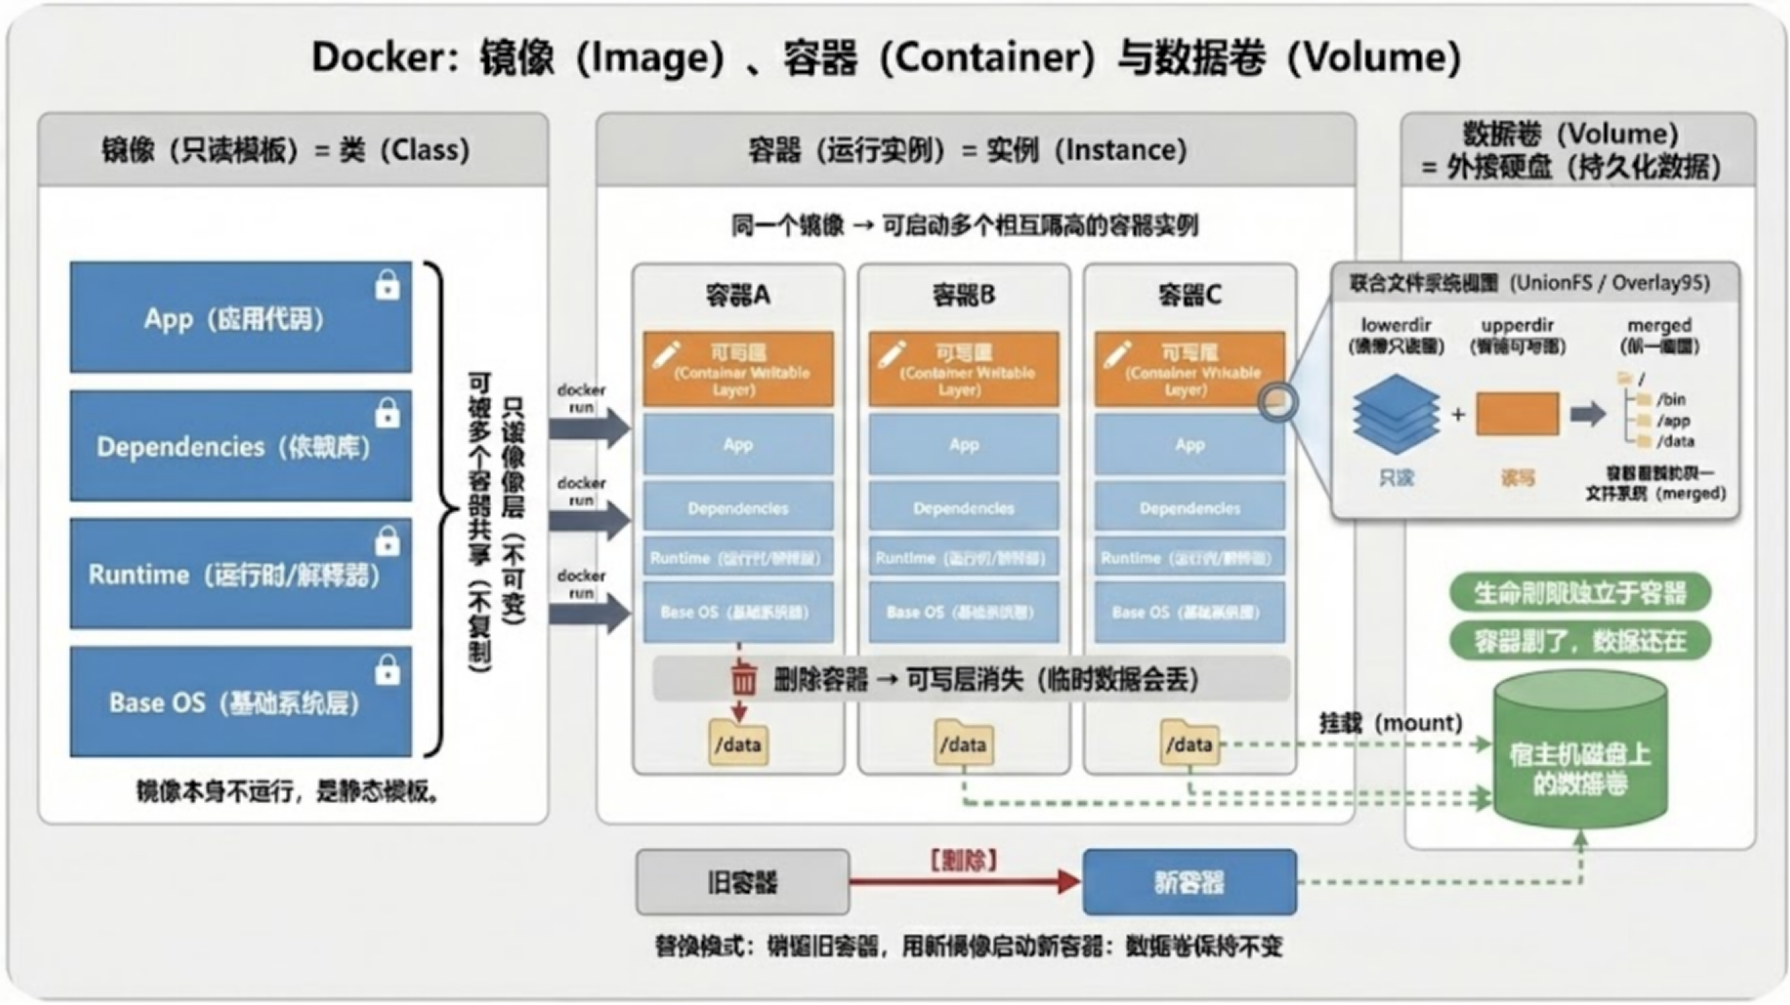
\includegraphics[width=1.0\textwidth]{figures/sec5/chapter5-2.png}
    \caption{镜像、容器以及数据卷}
    \label{fig:chapter5-2}
    \vspace{-15pt}
\end{figure*}

在Docker的概念体系中，有两个必须区分的核心概念：镜像（Image）与容器（Container）。它们的关系就是面向对象编程中"类"与"实例"的关系，或者说"程序"与"进程"的关系。

如图~\ref{fig:chapter5-2}所示，镜像是一份静态的、只读的系统快照，它完整记录了软件运行所需的一切：应用代码、依赖库、系统工具，乃至精简的操作系统用户空间。镜像一旦构建完成即不可篡改。容器则是镜像在宿主机上启动后的动态实例——一个被隔离的沙盒进程。基于同一个镜像可以启动多个容器，它们拥有独立的进程空间与网络环境，彼此隔离、互不干扰。

从系统实现的角度看，容器之所以能做到秒级启动且资源占用极低，秘密在于联合文件系统（UnionFS）的分层复用机制。观察图中容器A、B、C的内部结构：它们底部共享同一组只读的镜像层，Docker仅在其上挂载了一层薄薄的可写层。运行期间程序产生的所有状态变更——写日志、生成缓存、修改配置——都发生在这个可写层里，底下的镜像层始终保持只读。

这种设计带来一个必须警惕的副作用：可写层的生命周期与容器绑定。一旦容器被删除，可写层随之消失，其中的数据永久丢失。这就引出了一个工程问题：数据库文件、玩家存档这些需要持久保存的数据该放在哪里？

Docker的答案是数据卷（Volume）。如图~\ref{fig:chapter5-2}右侧所示，数据卷相当于一块挂载在容器上的"外接硬盘"。通过挂载操作，容器内部路径（如\texttt{/data}）被映射到宿主机磁盘上的一个目录。程序向这些路径写入数据时，数据流直接穿透可写层，落入宿主机磁盘。这样，计算逻辑（容器）与业务数据（卷）的生命周期就被彻底解耦——删除容器、升级镜像，只要挂载点不变，新容器依然能无缝接管之前的数据。

\subsubsection{隔离原理：Namespace与Cgroups}

\begin{figure*}[htbp]
    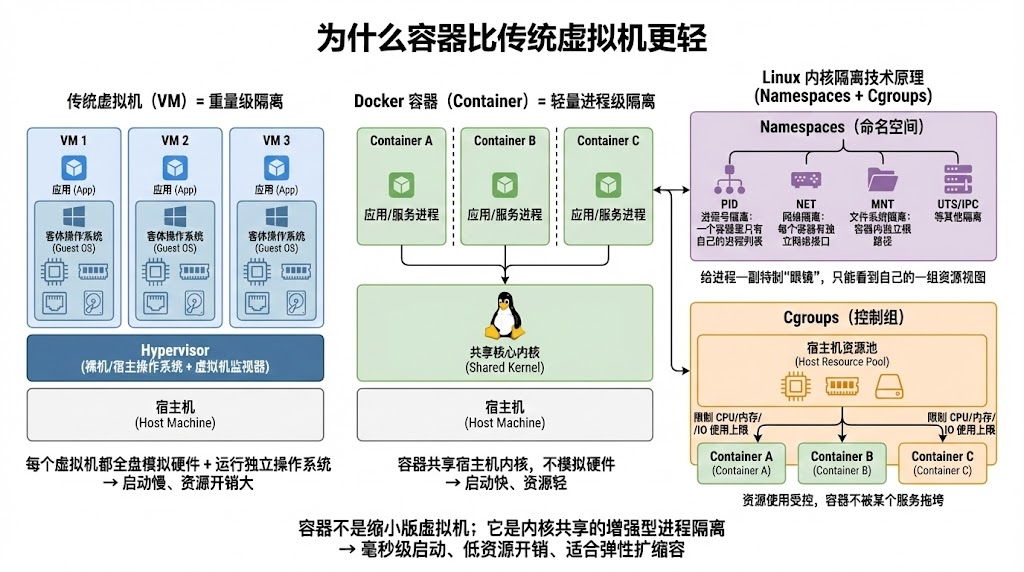
\includegraphics[width=1.0\textwidth]{figures/sec5/chapter5-3.png}
    \caption{容器与虚拟机的对比}
    \label{fig:chapter5-3}
    \vspace{-15pt}
\end{figure*}

容器能像虚拟机一样隔离运行服务，但为什么云计算普遍选择容器而非虚拟机？根本原因在于两者的隔离机制截然不同。

如图~\ref{fig:chapter5-3}左侧所示，传统虚拟机架构中每个实例都包含一套完整的Guest OS与模拟硬件层。这就像为了安顿一位客人，你得先建造一整栋独立的房子。反观图中间的容器架构，那层厚重的Guest OS彻底消失了，所有容器直接坐落在共享的宿主机内核之上。容器不需要重复启动内核，省去了漫长的开机自检与内存损耗，从而实现秒级启动与极低资源开销。

那么Docker如何让这些共享内核的进程"感觉"自己在独立运行？答案藏在图~\ref{fig:chapter5-3}右侧：Linux内核通过两大机制为进程构建隔离边界。

第一个是Namespace（命名空间）。它在PID（进程号）、NET（网络栈）、MNT（文件挂载点）等维度上为进程构建独立的视图：容器内部只能看到自己的进程列表和网络接口，完全感知不到宿主机上其他进程的存在。第二个是Cgroups（控制组）。它直接对接宿主机的资源池，严格限制每个容器能消耗的CPU时间片和内存上限，防止单个容器因资源失控而拖垮整台服务器。

理解了这两个机制，我们就能建立对容器最准确的直觉：容器不是"缩小版的虚拟机"，而是一个"自带隔离边界的增强型进程"。正是"共享内核"与"独占边界"的结合，让容器在保留隔离性的同时将资源利用率推向极致。

容器的网络隔离也依赖Namespace。Docker启动容器时，会把它放进独立的Network Namespace，容器内部看到的是自己专属的网络设备、IP地址和路由表。Docker通常为容器创建一对\texttt{veth}虚拟网卡——像一根"虚拟网线"的两端：一端放入容器的网络命名空间作为网络出口，另一端留在宿主机侧接入\texttt{docker0}网桥。同一宿主机上的多个容器通过\texttt{docker0}互联：数据包从源容器的\texttt{veth}端口进入网桥，再由网桥转发到目标容器的\texttt{veth}端口。

需要强调的是，容器与虚拟机在隔离强度上并不等价。容器共享宿主机内核，内核攻击面的隔离相对更弱；虚拟机为每个实例提供独立内核，边界更强但资源成本更高。在多租户云环境中，常见做法是引入gVisor、Kata Containers等轻量虚拟化方案，在性能与隔离之间取得折中。这些方案的原理将在第六章讨论。

\subsubsection{制作镜像：Dockerfile与分层构建}\label{sec:dockerfile}

\begin{figure*}[htbp]
    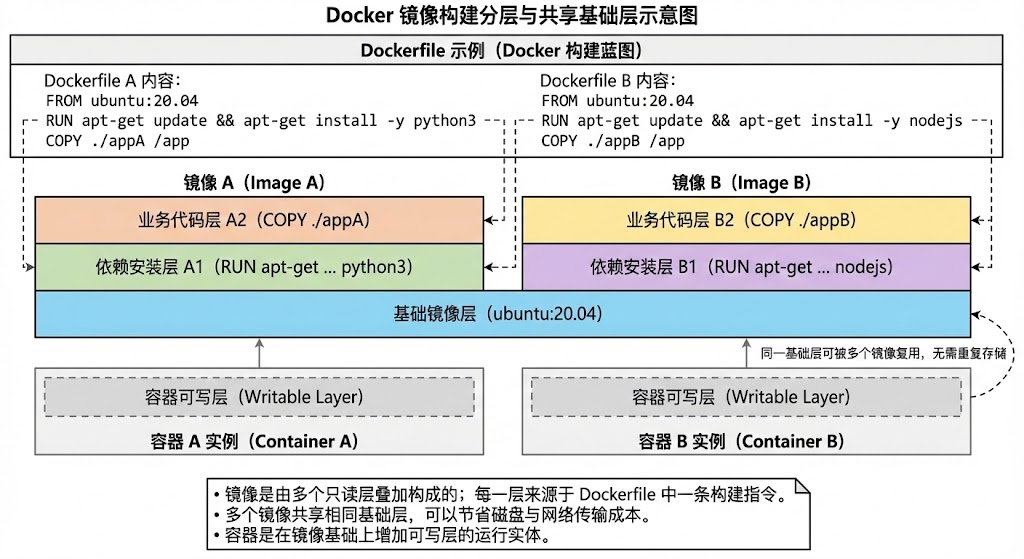
\includegraphics[width=1.0\textwidth]{figures/sec5/chapter5-1.png}
    \caption{Dockerfile构建镜像过程}
    \label{fig:chapter5-1}
    \vspace{-15pt}
\end{figure*}

镜像不是一个简单的压缩包，而是严格基于Dockerfile（构建蓝图）逐层生成的。如图~\ref{fig:chapter5-1}所示，Dockerfile中的每一行指令——无论是\texttt{FROM}定义的基础环境，还是\texttt{RUN}执行的软件安装——都会被转化为镜像中一个独立的只读层。这些层按指令顺序由下至上累积，每层仅记录相对于上一层的增量变化。

这种"指令即图层"的设计带来两个关键优势。第一是资源复用：如图中部蓝色区域所示，虽然镜像A与镜像B的上层业务代码不同，但它们共享同一个\texttt{ubuntu:20.04}基础层，物理存储上只需保存一份。部署大规模微服务时，系统仅需为各服务的差异部分"付费"，极大降低磁盘占用与网络传输成本。第二是构建缓存：Docker采用内容寻址存储（Content-Addressable Storage），每个镜像层由SHA256摘要唯一标识。只要某一层的输入没有变化，Docker就直接复用缓存而不重新构建，日常只改业务代码时通常只需重建最上面一两层。

回到我们的游戏项目。第四章中我们将后端拆分为大厅服与战斗服两个独立模块，未来还可能水平扩容（增开一区、二区）。如果为每个服务单独维护一份Dockerfile，维护成本会成倍攀升。下面这份通用Dockerfile通过构建参数实现了"一份蓝图，多个服务"的复用：

\begin{tcolorbox}[title=通用Dockerfile：多阶段构建]
\begin{lstlisting}[language=bash,basicstyle=\ttfamily\footnotesize,numbers=left,numberstyle=\tiny\color{gray},numbersep=5pt,aboveskip=0pt,belowskip=0pt,lineskip=-1pt,commentstyle=\color{gray},keywordstyle=\color{blue}\bfseries,breaklines=true,showstringspaces=false]
FROM golang:1.21-alpine AS builder
WORKDIR /app
COPY go.mod go.sum ./
RUN go mod download
COPY . .
ARG SERVICE
RUN if [ -z "$SERVICE" ]; then echo "ERR: SERVICE not set"; exit 1; fi
RUN CGO_ENABLED=0 GOOS=linux go build -o server_bin ./cmd/${SERVICE}
FROM alpine:latest
RUN apk --no-cache add ca-certificates tzdata
WORKDIR /root/
COPY --from=builder /app/server_bin .
COPY --from=builder /app/config ./config
CMD ["./server_bin"]
\end{lstlisting}
\end{tcolorbox}

这份Dockerfile的核心不在于命令语法，而在于三个工程决策。其一，多阶段构建：第一阶段（\texttt{builder}）使用包含Go工具链的完整编译环境（约300\,MB），第二阶段切换到仅5\,MB的Alpine基础镜像，只从第一阶段复制编译产物。最终镜像通常只有10--15\,MB，扩容时节点拉取镜像的时间显著缩短。其二，依赖缓存优化：先复制\texttt{go.mod}与\texttt{go.sum}并下载依赖，再复制源码。由于依赖变动频率远低于业务代码，这种顺序能最大化缓存命中率。其三，静态编译：\texttt{CGO\_ENABLED=0}生成的二进制自带所有依赖，不依赖宿主机的动态链接库，这也是容器能运行在极简环境中的前提。关于每行指令的详细解读，请参见附录~\ref{sec:appendix-dockerfile}。

\subsubsection{分发镜像：Registry与版本锁定}

\begin{figure*}[htbp]
    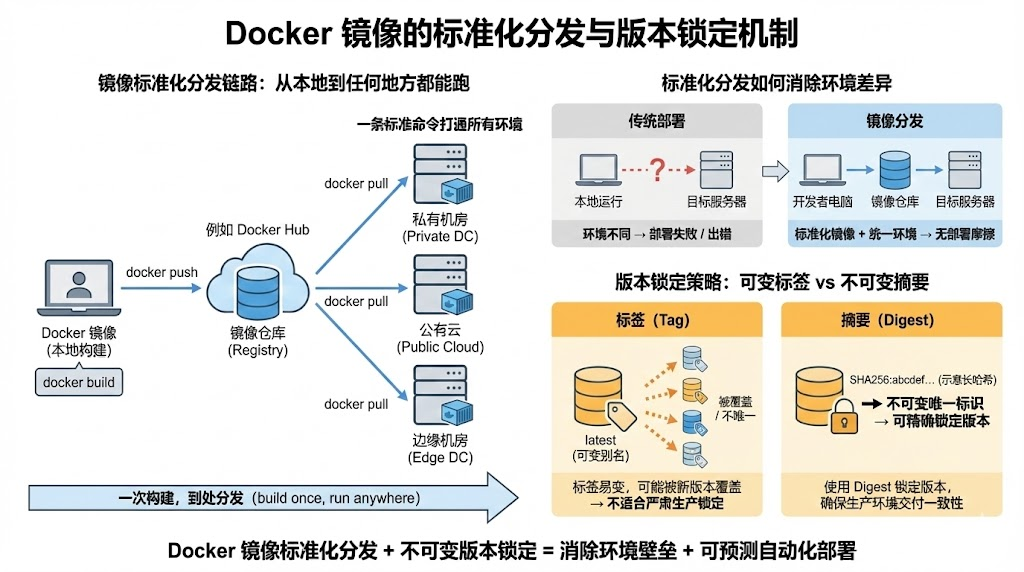
\includegraphics[width=1.0\textwidth]{figures/sec5/chapter5-4.png}
    \caption{Docker的标准化分发链路}
    \label{fig:chapter5-4}
    \vspace{-15pt}
\end{figure*}

镜像构建完成后，如何让三台云服务器都能拿到同一份镜像？Docker通过镜像仓库（Registry）机制解决这个问题。如图~\ref{fig:chapter5-4}所示，开发者用\texttt{docker push}将镜像推送到远端仓库（如Docker Hub或云厂商的私有仓库），运维人员在任意服务器上用\texttt{docker pull}即可将完整的运行环境原样拉取下来。Docker的分层机制确保只上传云端缺失的增量层，节省带宽。

在生产环境中，版本锁定是一个容易被忽视但至关重要的环节。Docker提供了\texttt{latest}等标签（Tag）机制，但标签本质上是可变的别名——今天拉取的\texttt{latest}和明天拉取的可能是完全不同的代码。因此工程实践中更倾向于使用镜像摘要（Digest），即对镜像内容进行SHA256哈希计算生成的唯一标识符。通过摘要锁定版本，可以确保无论何时何地拉取，得到的都是同一份镜像。

下面是完整的镜像发布流程：

\begin{tcolorbox}[title=镜像发布与版本锁定]
\begin{lstlisting}[language=bash,basicstyle=\ttfamily\footnotesize,numbers=left,numberstyle=\tiny\color{gray},numbersep=5pt,aboveskip=0pt,belowskip=0pt,lineskip=-1pt,commentstyle=\color{gray},keywordstyle=\color{blue}\bfseries,breaklines=true,showstringspaces=false]
docker build -t game-lobby:v1 .                        # 构建镜像
docker login                                            # 登录镜像仓库
docker tag game-lobby:v1 username/game-lobby:v1         # 打标签
docker push username/game-lobby:v1                      # 推送到云端
docker pull username/game-lobby@sha256:[digest]         # 按摘要拉取
docker images --digests                                 # 验证一致性
\end{lstlisting}
\end{tcolorbox}

至此，我们解决了单个容器的标准化交付问题：从构建、分发到版本锁定，形成了一条完整的流水线。但现实中的游戏后端不止一个服务——大厅服、战斗服、Redis、MySQL、Nginx至少五个组件需要协同启动。手动逐个\texttt{docker run}不仅繁琐，而且启动顺序、网络互联、配置传递都容易出错。下一节我们用Docker Compose来解决这个问题。


\subsection{多容器编排：用Compose一键开服}

\subsubsection{手工启动的痛苦}

回想第四章构建的分布式架构，我们至少有网关服务、战斗服务、Redis缓存和MySQL数据库四个组件。要让游戏后端运行起来，必须协调启动多个容器，并保证启动顺序、网络连接和配置传递正确无误。如果用手工方式，流程大致如下：

\begin{tcolorbox}[title=手工启动多个容器]
\begin{lstlisting}[language=bash,basicstyle=\ttfamily\footnotesize,numbers=left,numberstyle=\tiny\color{gray},numbersep=5pt,aboveskip=0pt,belowskip=0pt,lineskip=-1pt,commentstyle=\color{gray},keywordstyle=\color{blue}\bfseries,breaklines=true,showstringspaces=false]
docker run -d --name mysql-db -e MYSQL_ROOT_PASSWORD=123456 mysql
docker run -d --name redis-cache redis
docker run -d --name map-service --link mysql-db -p 8081:8080 game/map-service
docker run -d --name gateway --link map-service -p 8080:8080 game/gateway
\end{lstlisting}
\end{tcolorbox}

四个容器就需要四条命令，必须严格按顺序执行，还要手动处理端口映射和容器间链接。每次发布、每次更新都要重复这套流程，稍有疏忽就可能导致连接失败或服务不可用。

\subsubsection{Compose的声明式配置}

\begin{figure}[htbp]
\centering

\includegraphics[width=0.85\textwidth]{figures/sec5/Docker_Compose_concepts.png}
\caption{Docker Compose服务编排的核心概念与工作机制}
\label{fig:compose-concepts}
\end{figure}

Docker Compose通过一份YAML格式的声明式配置文件，将上述所有手工操作收敛为一条命令：\texttt{docker-compose up -d}。如图~\ref{fig:compose-concepts}所示，配置文件清晰描述了所有服务的镜像、端口映射、环境变量、依赖关系和网络设置。

\begin{tcolorbox}[title=Docker Compose配置示例]
\begin{lstlisting}[language=bash,basicstyle=\ttfamily\footnotesize,numbers=left,numberstyle=\tiny\color{gray},numbersep=5pt,aboveskip=0pt,belowskip=0pt,lineskip=-1pt,commentstyle=\color{gray},keywordstyle=\color{blue}\bfseries,breaklines=true,showstringspaces=false]
version: "3"
services:
  mysql-db:
    image: mysql:5.7
    environment:
      MYSQL_ROOT_PASSWORD: "123456"
    ports:
      - "3306:3306"
    volumes:
      - db-data:/var/lib/mysql
  redis-cache:
    image: redis:6
    ports:
      - "6379:6379"
  map-service:
    image: game/map-service:v1
    depends_on:
      - mysql-db
      - redis-cache
    ports:
      - "8081:8080"
    environment:
      DB_HOST: mysql-db
      REDIS_HOST: redis-cache
  gateway-service:
    image: game/gateway:v1
    depends_on:
      - map-service
    ports:
      - "8080:8080"
    environment:
      MAP_SERVICE_HOST: map-service
volumes:
  db-data:
\end{lstlisting}
\end{tcolorbox}

执行\texttt{docker-compose up}时，Compose首先解析配置文件并验证语法，然后根据\texttt{depends\_on}字段构建服务间的依赖关系图（一个有向无环图），对其进行拓扑排序以确定启动顺序。接着Compose创建一个专属的虚拟网络，并为每个服务配置DNS解析——在这个网络中，容器可以直接通过服务名（如\texttt{mysql-db}）访问其他容器，无需知道具体IP地址。最后按拓扑顺序逐个启动容器，自动完成镜像拉取、环境变量注入、端口映射和网络接入。

\begin{figure}[htbp]
\centering
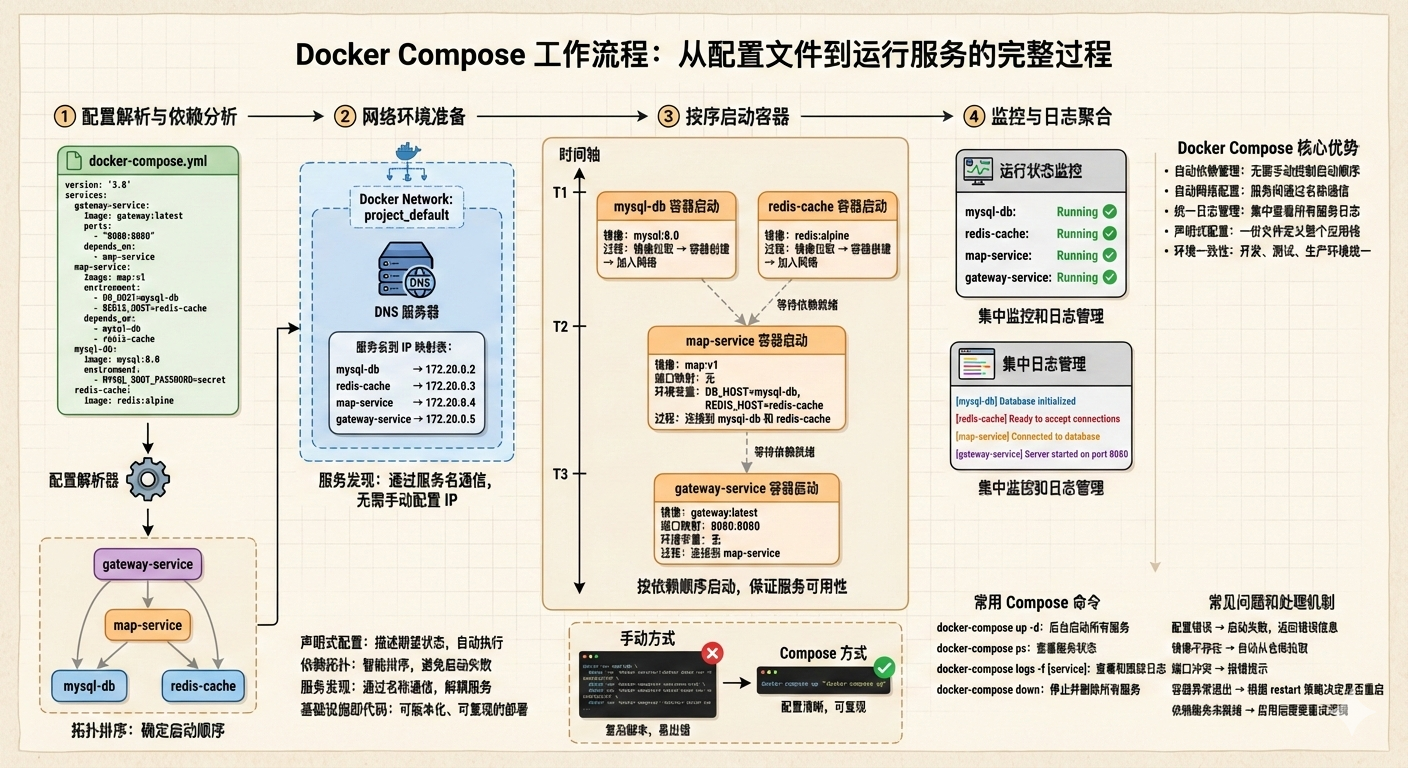
\includegraphics[width=0.9\textwidth]{figures/sec5/docker-compose-workflow.png}
\caption{Docker Compose工作流程：从配置文件到运行服务}
\label{fig:compose-workflow}
\end{figure}

这里有两个细节值得注意。第一，\texttt{depends\_on}只保证容器的启动顺序，不等待服务真正就绪。例如MySQL容器已经启动，但数据库服务本身可能还在初始化，尚未准备好接受连接。应用代码需要实现重试逻辑来应对这种情况。第二，Compose的声明式配置天然具备幂等性：反复执行\texttt{docker-compose up}时，Compose会比对当前状态与配置文件的期望状态，只进行必要的创建或重建操作，不会产生重复容器或端口冲突。

对于需要长期运行的游戏服务，Compose还提供了重启策略：\texttt{restart: always}表示无论何种退出都自动拉起，\texttt{on-failure}只在非零退出码时重启，\texttt{unless-stopped}则尊重人工停机操作。这些策略虽然简单，却已经体现出自愈机制的雏形。

\subsubsection{Compose的边界：为什么单机编排不够}

当项目从几百名在线玩家增长到上千甚至更多时，Compose的局限性会迅速显现。它本质上依赖单一Docker Engine，所有容器集中在一台机器上运行。这意味着：一旦主机硬件故障，服务整体不可用；缺乏跨节点调度能力，无法把负载分散到多台服务器；不具备滚动更新机制，版本发布时容易引入可感知中断；没有面向实时负载的自动伸缩控制，难以应对突发流量。

这些限制并非Compose的设计缺陷——它本来就是为单机开发和测试场景设计的。当我们需要跨多台机器调度容器、自动故障恢复、滚动发布和弹性伸缩时，就需要一个真正的集群编排系统。这正是Kubernetes要解决的问题。

\subsection{Kubernetes：集群级的自动化编排}

\subsubsection{从Compose到K8s：新的问题域}

Compose解决了单机上多容器的协同启动问题，但当我们把视野从一台机器扩展到十台、五十台时，一组全新的问题浮出水面。

第一，调度问题：新启动的容器应该放在哪台机器上？需要综合考虑各节点的剩余CPU、内存、网络带宽，以及容器之间的亲和性约束。第二，故障恢复：某台服务器宕机后，上面运行的容器怎么办？需要自动在其他健康节点上重新启动。第三，滚动更新：发布新版本时，如何做到不中断服务？需要逐步替换旧容器，确保任何时刻都有足够的实例在处理请求。第四，服务发现：容器的IP地址随时可能因为重启或迁移而变化，其他服务如何找到它？

这四个问题的共同特征是：它们都超出了单机的范畴，需要一个拥有全局视野的"指挥中心"来统一协调。Kubernetes（简称K8s）正是这样一个系统。

\subsubsection{核心概念：Pod、Deployment、Service}

\begin{figure}[htbp]
\centering
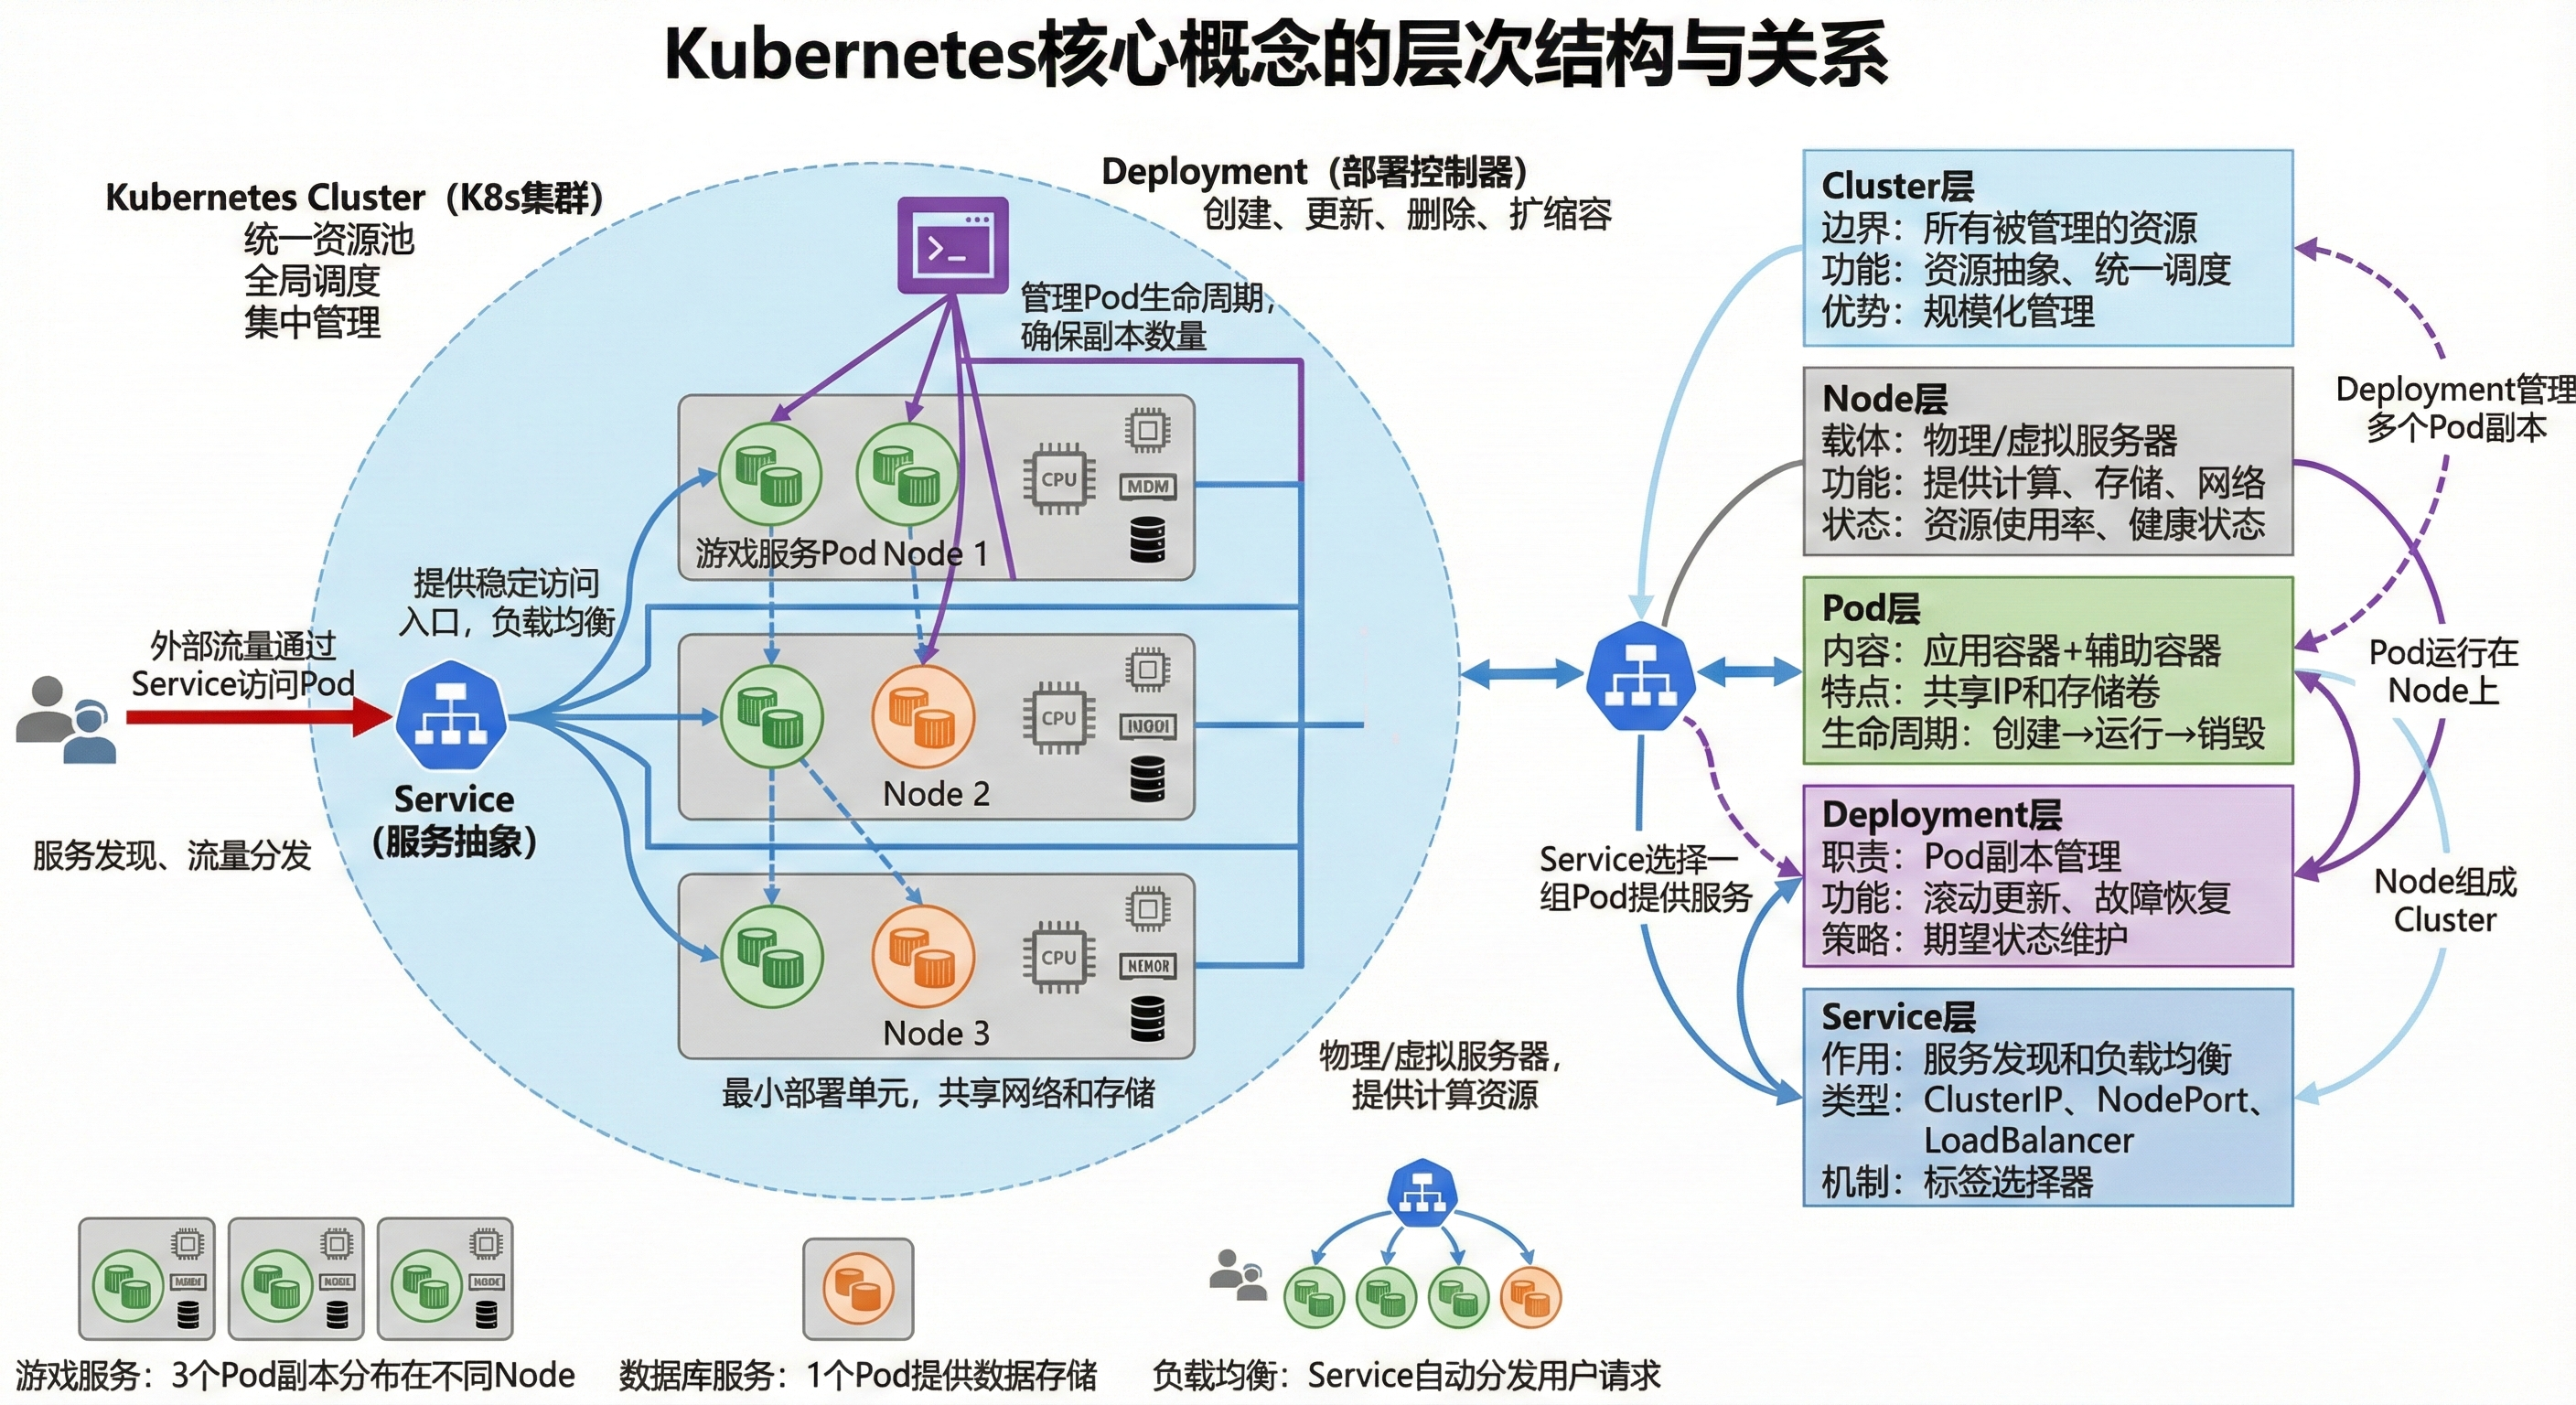
\includegraphics[width=0.9\textwidth]{figures/sec5/kubernetes-architecture-concepts.png}
\caption{Kubernetes核心概念的层次结构与关系}
\label{fig:k8s-concepts}
\end{figure}

Kubernetes的概念体系可以从底向上理解。如图~\ref{fig:k8s-concepts}所示：

\textbf{Node}（节点）是集群中的一台物理服务器或云主机，提供CPU、内存和网络等计算资源。\textbf{Pod}是K8s中最小的部署单元，通常包含一个主应用容器和可选的辅助容器（如日志收集），它们共享网络和存储，必须调度到同一个Node上运行。\textbf{Deployment}负责管理Pod的生命周期——确保始终有期望数量的Pod在健康运行，某个Pod故障时自动创建替代品，版本更新时协调滚动替换。\textbf{Service}为一组功能相同的Pod提供统一的访问入口和负载分发，外部请求通过Service到达后端Pod，无需知道具体哪个Pod在处理。

这套概念与第四章的架构有直接的对应关系。第四章中我们手工维护Nginx的\texttt{upstream}列表来实现负载均衡，每次后端实例变化都要改写配置并执行\texttt{nginx -s reload}。在K8s中，Service基于Pod的标签（Label）持续观察成员变化，由kube-proxy组件自动刷新端点列表——不再需要手动维护服务器清单。第四章的协调服务器负责服务注册与发现，在K8s中这个职责下沉为基础设施能力：CoreDNS为每个Service自动生成域名（如\texttt{game-server.default.svc.cluster.local}），集群内任何Pod都可以通过域名直接访问其他服务。

下面是一个完整的K8s配置示例，定义了一个运行三个副本的游戏服务及其负载均衡入口：

\begin{tcolorbox}[title=Kubernetes部署配置]
\begin{lstlisting}[language=bash,basicstyle=\ttfamily\footnotesize,numbers=left,numberstyle=\tiny\color{gray},numbersep=5pt,aboveskip=0pt,belowskip=0pt,lineskip=-1pt,commentstyle=\color{gray},keywordstyle=\color{blue}\bfseries,breaklines=true,showstringspaces=false]
apiVersion: apps/v1
kind: Deployment
metadata:
  name: game-server
spec:
  replicas: 3
  selector:
    matchLabels:
      app: game
  template:
    metadata:
      labels:
        app: game
    spec:
      containers:
      - name: game-server
        image: game/server:v1
        ports:
        - containerPort: 8080
        resources:
          requests:
            memory: "512Mi"
          limits:
            memory: "1Gi"
---
apiVersion: v1
kind: Service
metadata:
  name: game-service
spec:
  selector:
    app: game
  ports:
  - protocol: TCP
    port: 80
    targetPort: 8080
  type: LoadBalancer
\end{lstlisting}
\end{tcolorbox}

一条命令\texttt{kubectl apply -f deployment.yaml}，K8s就会自动完成调度、部署、负载均衡和健康检查。这份配置的关键在于它是声明式的：我们描述的是"期望状态"（3个副本、每个512Mi内存），而非"执行步骤"。

\subsubsection{声明式管理与Reconciliation Loop}

\begin{figure}[htbp]
\centering
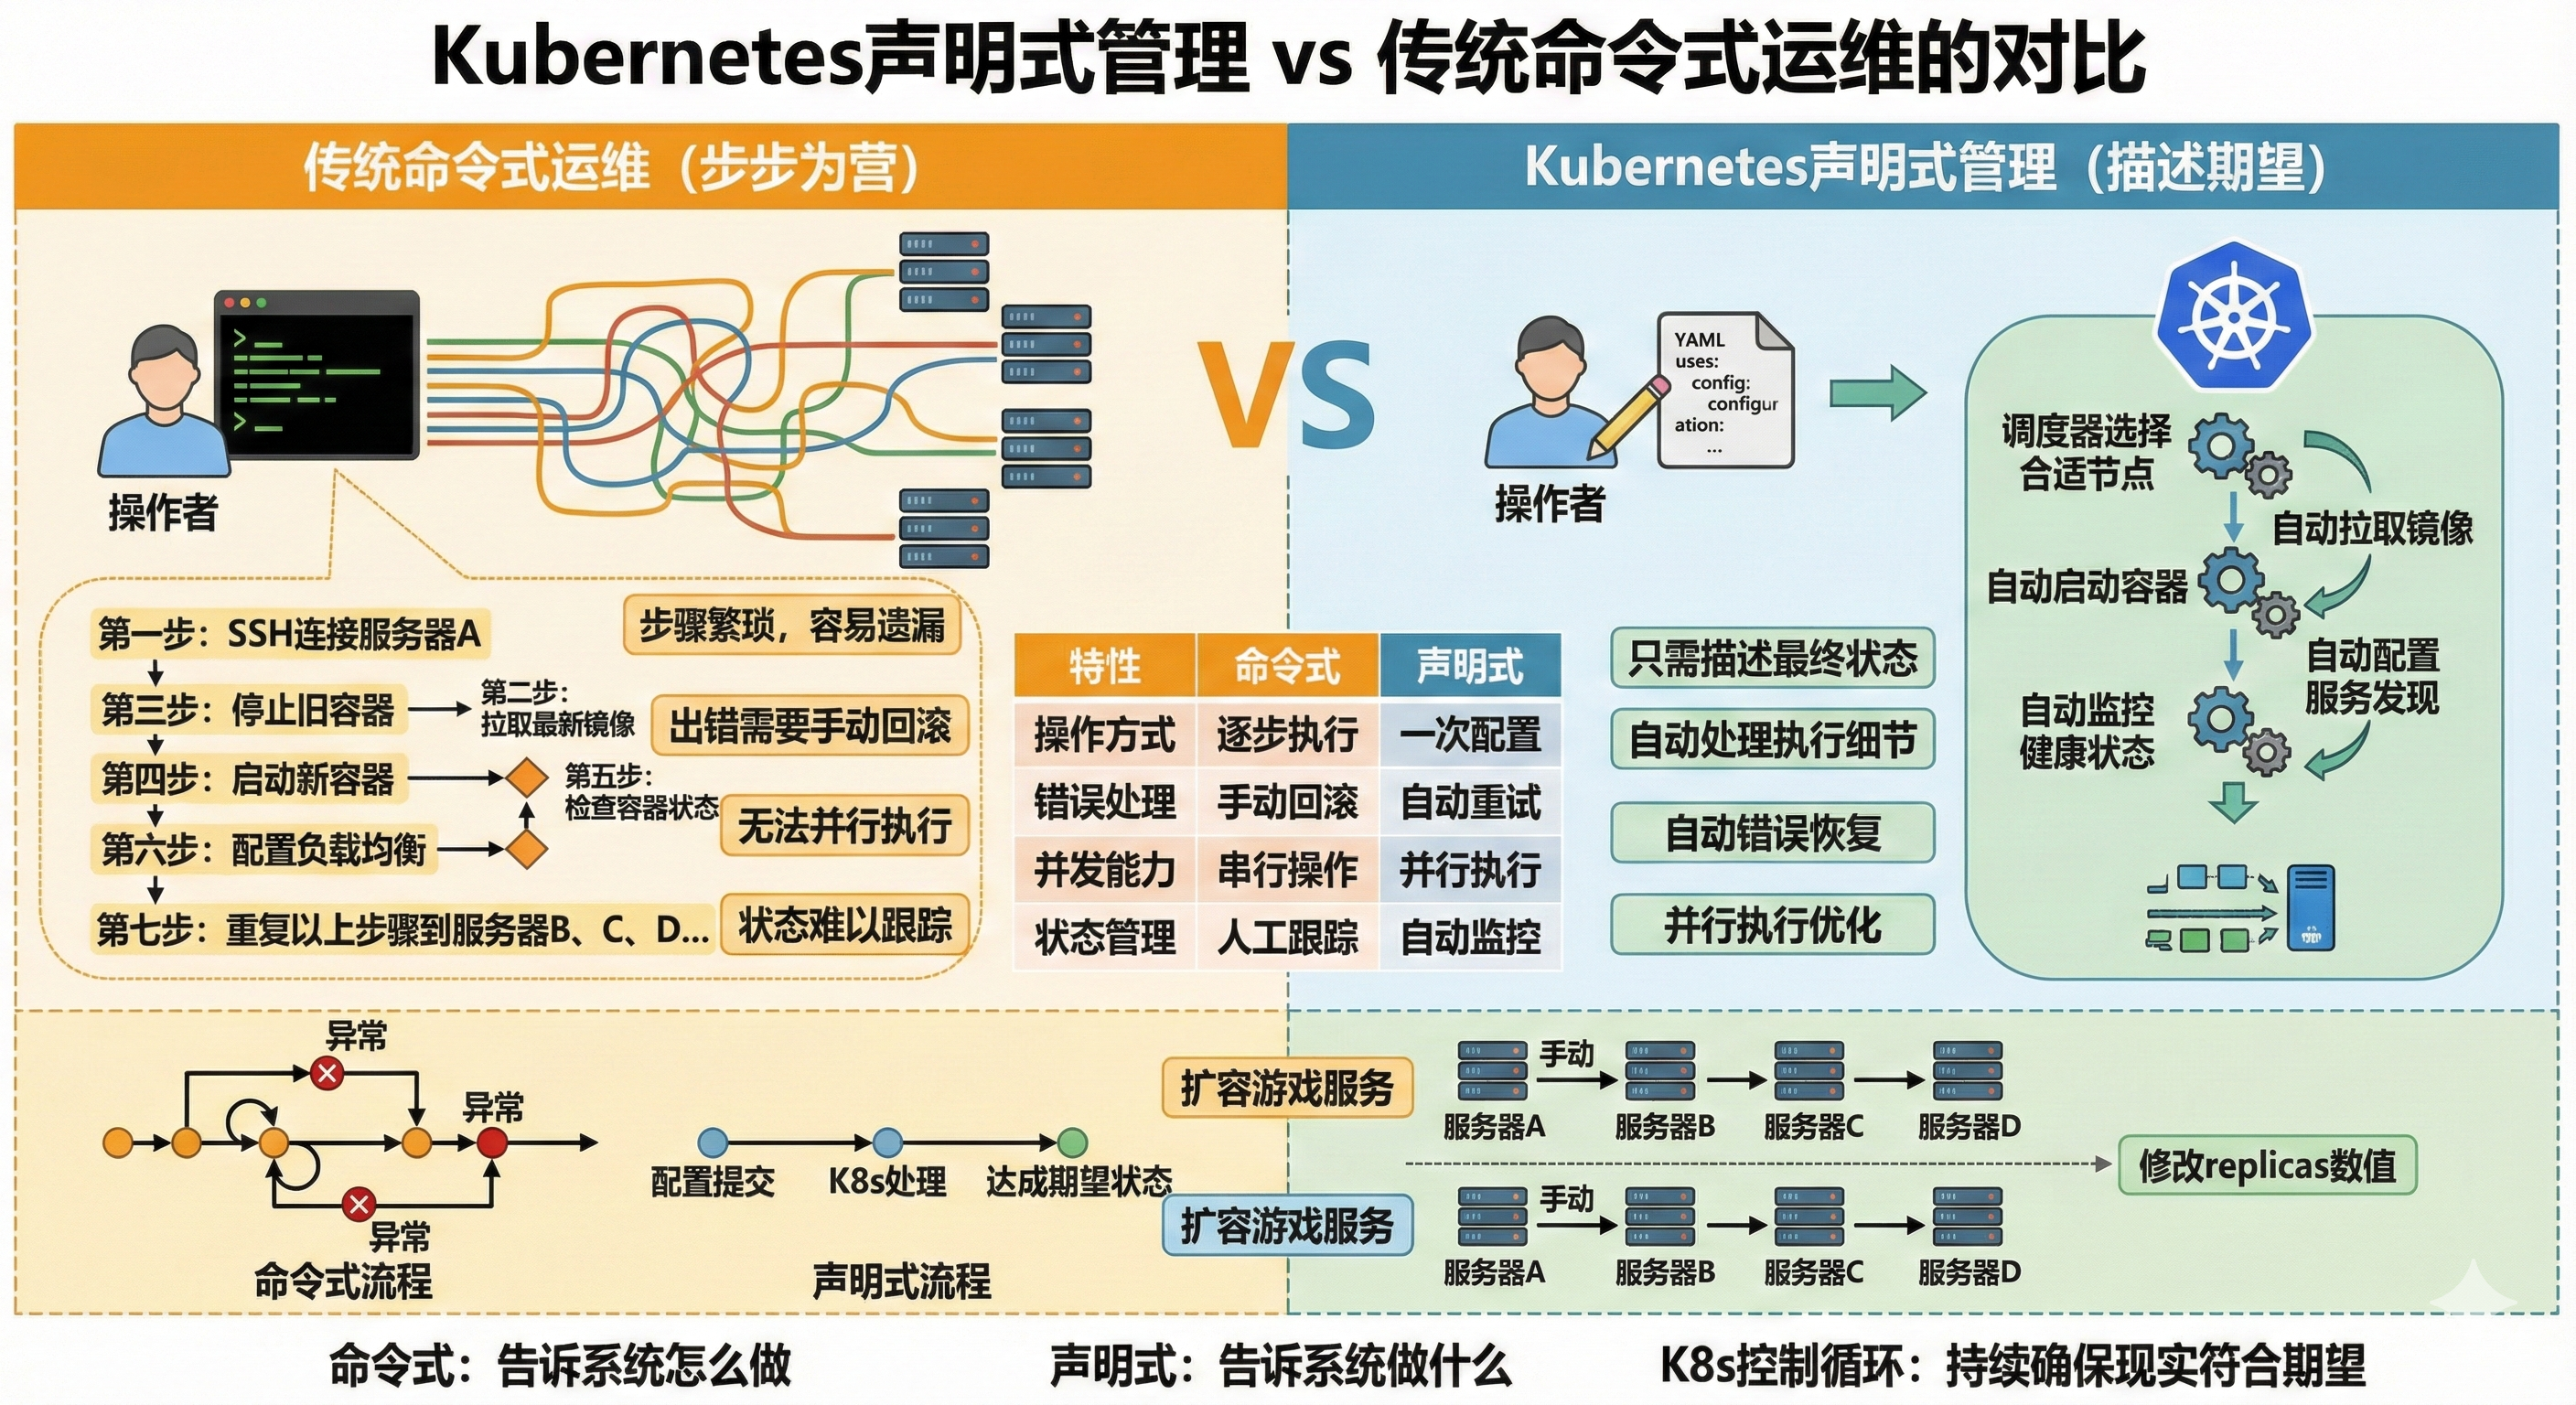
\includegraphics[width=0.9\textwidth]{figures/sec5/kubernetes-declarative-vs-imperative.png}
\caption{声明式管理与命令式运维的对比}
\label{fig:declarative-vs-imperative}
\end{figure}

声明式管理是K8s最核心的设计哲学。如图~\ref{fig:declarative-vs-imperative}所示，传统的命令式运维要求你明确指定每一个执行步骤："在服务器A上启动容器X，在服务器B上启动容器Y，配置负载均衡器指向这两个容器"。而K8s的声明式方式只需描述期望的最终状态："我需要3个游戏服务器副本在运行"，系统自动分析当前状态与期望状态的差异并执行必要操作。

这种设计的关键不在于"一次下发命令"，而在于持续运行的Reconciliation Loop（调谐循环）。控制器不断执行"观察现状、对比期望、采取动作、再次观察"的闭环，使系统逐步逼近期望状态。这属于Level-triggered思路——关注的是"现在是否达标"，而非"刚刚发生了什么事件"。即便某次消息丢失或某个操作失败，下一轮循环仍会重新发现偏差并自动修正。系统的鲁棒性来自反复校准，而非假设每条通知都可靠送达。

用游戏场景来讲：运营者只需声明"城门始终保持3名守卫"，某个守卫倒下后，控制逻辑会在后续轮次自动补位，而不需要人工逐条下达替补指令。当你需要扩容时，只需把"3"改成"10"，K8s会自动启动7个新Pod；当你需要更新版本时，只需修改镜像标签，K8s会自动执行滚动更新，逐步替换旧Pod，确保服务不中断。

\subsubsection{调度与健康检查}

当一个新Pod需要启动时，K8s的调度器负责决定它应该运行在哪个Node上。调度过程分为两个阶段：先做过滤（Filter），根据资源请求、亲和与反亲和规则、污点容忍等约束剔除不合适的Node；再做打分（Score），对候选Node按剩余资源、负载均衡度等指标评分排序，选择当前最优者。

从理论上看，这本质上是一个多维资源装箱问题——CPU、内存、带宽与拓扑同时参与决策，计算复杂性通常被视为NP-hard，因此工程实现强调近似最优与可扩展性。其思想脉络可追溯到Google的Borg系统，随后发展到Omega，再到今天的Kubernetes。用游戏比喻：调度器像在给玩家分配房间，不只看空位多少，还要兼顾延迟、容量与地域。

Pod启动后，K8s通过探针（Probe）机制持续监控其健康状态。还记得第四章中我们为游戏服务器实现的健康检查端点吗？协调服务器定期发送HTTP请求，连续几次无响应就将其从可用列表中移除。K8s采用同样的思路，但拆分为两类探针：\textbf{Liveness Probe}检测进程是否"活着但已失效"（如死锁），触发容器重启；\textbf{Readiness Probe}检测实例是否已准备好接收流量，未就绪时将其临时移出Service的负载均衡池。核心思想不变，只是由平台统一执行，而非业务代码重复实现。

\begin{figure}[htbp]
\centering
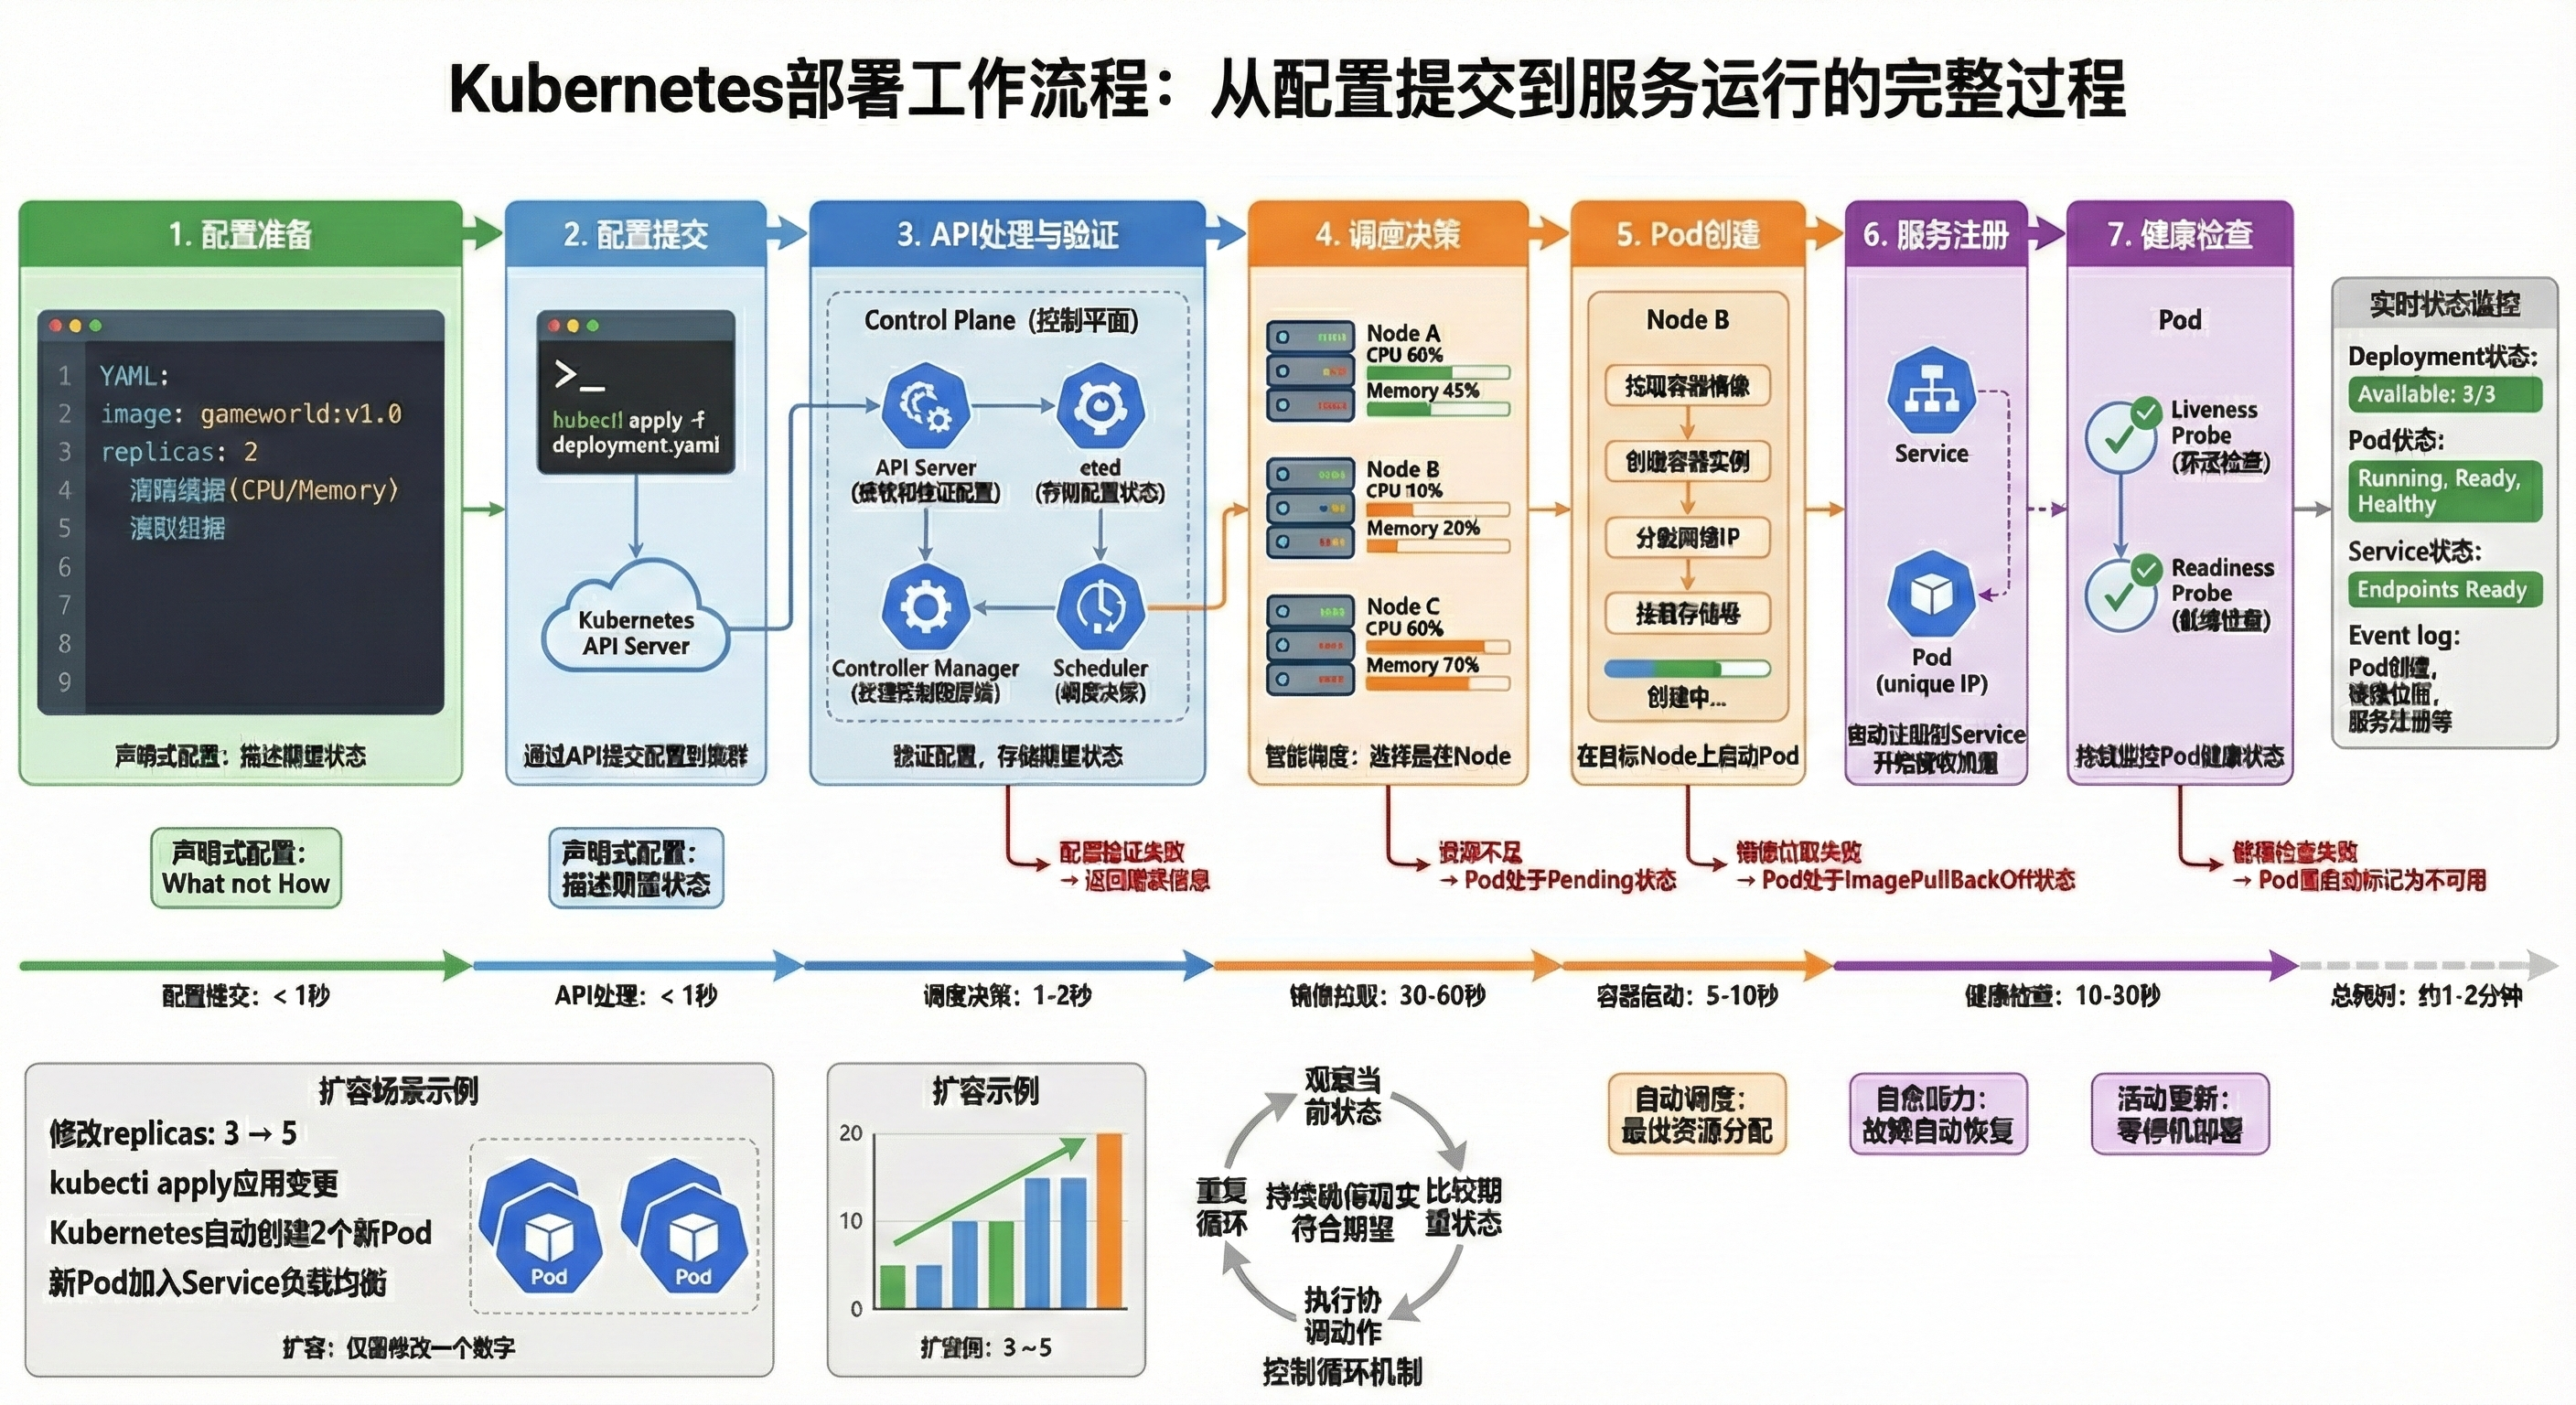
\includegraphics[width=0.9\textwidth]{figures/sec5/kubernetes-deployment-workflow.png}
\caption{Kubernetes部署工作流程：从配置提交到服务运行}
\label{fig:k8s-workflow}
\end{figure}

如图~\ref{fig:k8s-workflow}所示，从配置提交到服务稳定运行，整个过程是高度自动化的闭环：调度器选择Node，kubelet启动容器，探针监控健康状态，Service自动更新端点列表。当某个Pod异常退出时，Deployment控制器立即启动替代Pod，调度器为其选择合适的Node，整个恢复过程无需人工干预。

理解了上述核心概念后，读者可以参照附录~\ref{sec:appendix-k8s-deploy}的实战指南，亲手完成从编写YAML配置、执行\texttt{kubectl apply}到监控部署状态的完整流程。

\subsubsection{游戏服务的特殊挑战}

在将游戏后端迁移到K8s的过程中，有几个游戏场景特有的问题值得专门讨论。

第一个是协议选择。实时战斗场景对延迟和抖动极为敏感，核心链路通常选用UDP以避免TCP的队头阻塞。K8s的Service对UDP是原生支持的，端口声明后即可进行四层转发与负载分担。但需要注意，常见的Nginx Ingress主要工作在HTTP/HTTPS语义层，默认不能直接代理通用UDP流量。生产环境中更稳妥的做法是为游戏服单独创建\texttt{type: LoadBalancer}的Service，由云厂商的负载均衡器直接暴露UDP四层入口。这里要区分L4与L7负载均衡：前者按传输层五元组转发，后者理解应用层协议与路由规则。游戏业务在网关设计时应先确定协议边界，再决定在哪一层实施流量治理。

第二个是有状态问题。Deployment的设计假设是无状态工作负载——任何Pod都可以被随时替换。这对大多数Web服务很合适，但游戏服务端往往在内存中维护玩家会话：第三章连接池模型里保存的连接上下文、匹配状态与短期战斗数据，都绑定在当前进程上。工程上常见两条路：

其一，将会话状态外置到Redis等外部存储，让业务Pod回到可替换的无状态形态。这更符合云原生的弹性与故障恢复思路，但每次读写状态都引入额外的网络时延与一致性成本。其二，采用StatefulSet为Pod提供稳定的网络标识与持久命名，配合Session Affinity将特定玩家的流量固定到特定Pod。这更接近传统游戏分区服架构，迁移门槛低，但会牺牲调度自由度与横向伸缩效率。

两种方案各有适用场景，没有绝对的优劣。对于登录、匹配等无状态服务，状态外置是自然选择；对于需要将玩家"粘"在特定战斗实例上的有状态场景，StatefulSet加会话亲和更为务实。这两类方案的容量评估与故障演练方法将在第六章进一步展开。

\subsection{弹性伸缩：让资源跟着玩家走}

在第四章中，当玩家负载增加时，我们的应对方式是：手动开通新的云服务器，部署游戏服务，向协调服务器注册，再修改Nginx配置。负载下降需要缩容时更加麻烦：必须先迁移玩家、确认没有活跃会话后才能安全关闭。扩缩容的每一步都需要人工操作和业务逻辑配合。

在K8s的世界里，思路完全不同：你只需声明"我希望CPU使用率保持在70\%以下"，平台就会自动增减Pod实例，Service自动调整流量分发。扩缩容从"人工操作服务器"变成了"声明期望状态"。

\subsubsection{问题：固定配置遇上波动流量}

\begin{figure}[htbp]
\centering
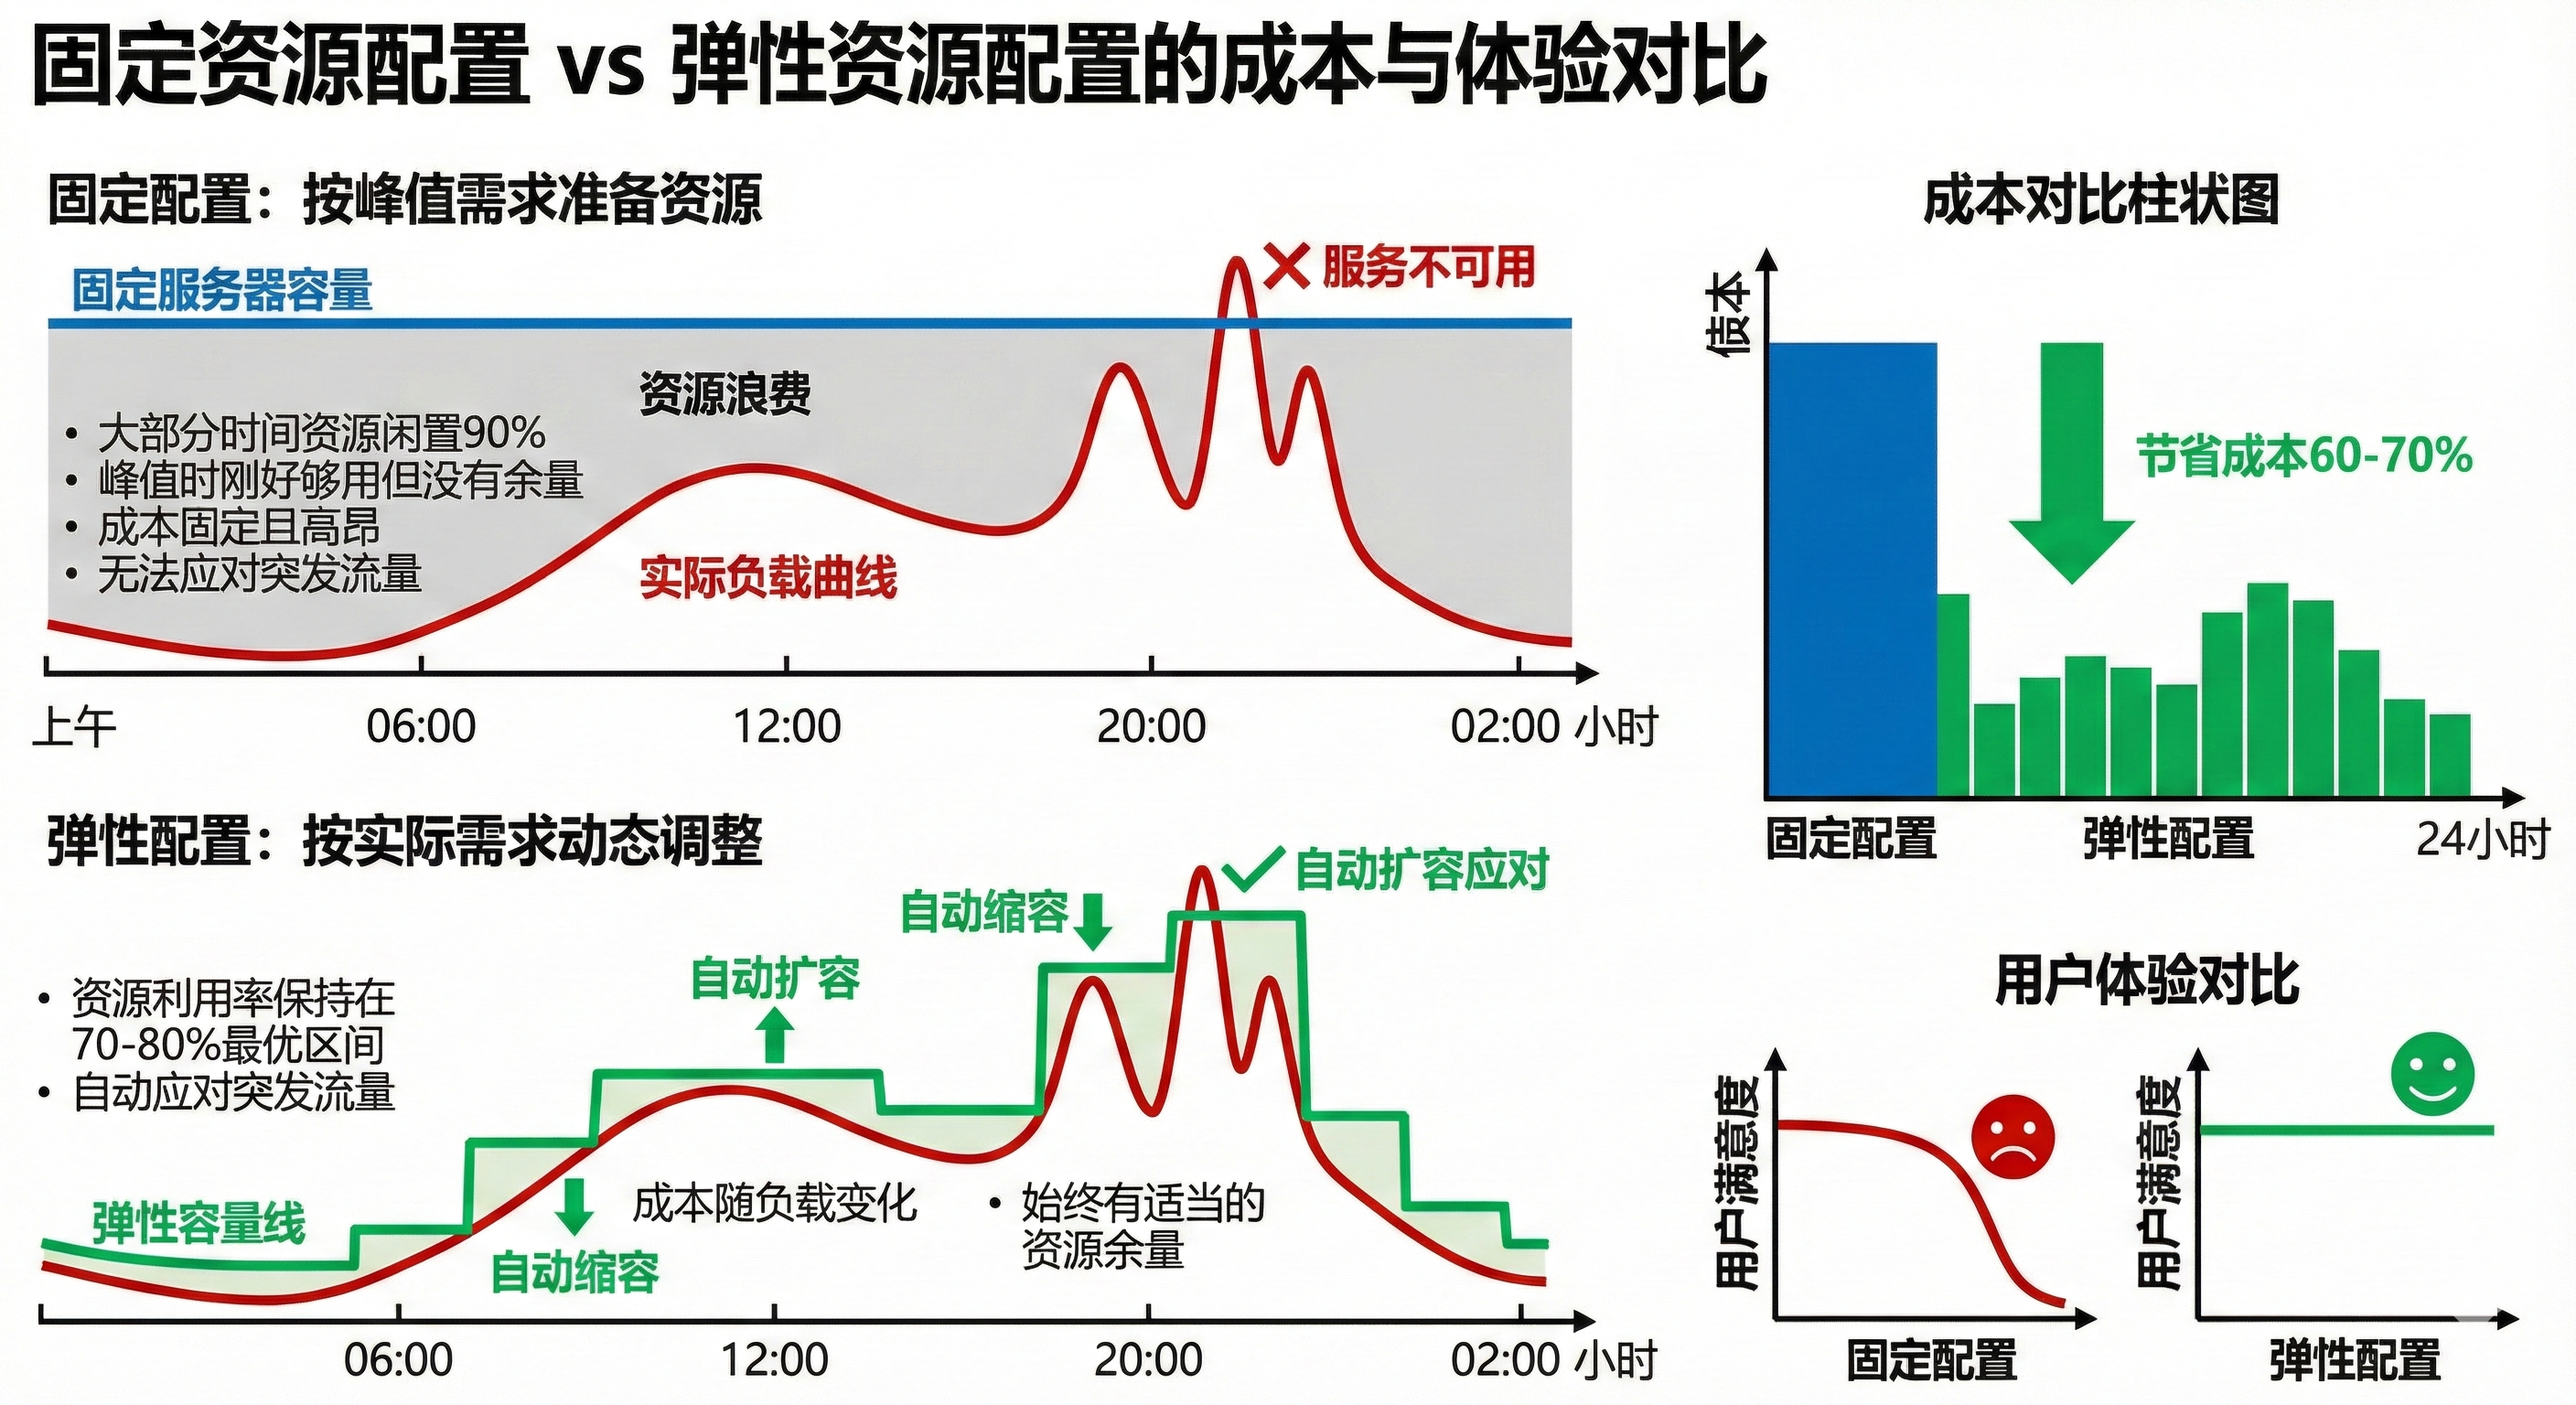
\includegraphics[width=0.9\textwidth]{figures/sec5/fixed-vs-elastic-resources.png}
\caption{固定资源配置与弹性资源配置的成本与体验对比}
\label{fig:fixed-vs-elastic}
\end{figure}

传统部署模式按业务高峰期配置服务器数量。如图~\ref{fig:fixed-vs-elastic}所示，这种策略面临结构性矛盾：周五晚上8点同时在线5万人，需要50台服务器；周二上午10点在线5000人，5台就够了。如果始终维持50台，90\%的时间里大部分资源在空转；如果按平均流量配置，高峰期就会出现连接超时和操作卡顿。

更棘手的是突发流量：一个主播的推荐、一次版本更新的热度，都可能在几分钟内让负载暴增数十倍。静态配置无法应对这种不可预测的波动。

\subsubsection{HPA：Pod级自动扩缩}

\begin{figure}[htbp]
\centering
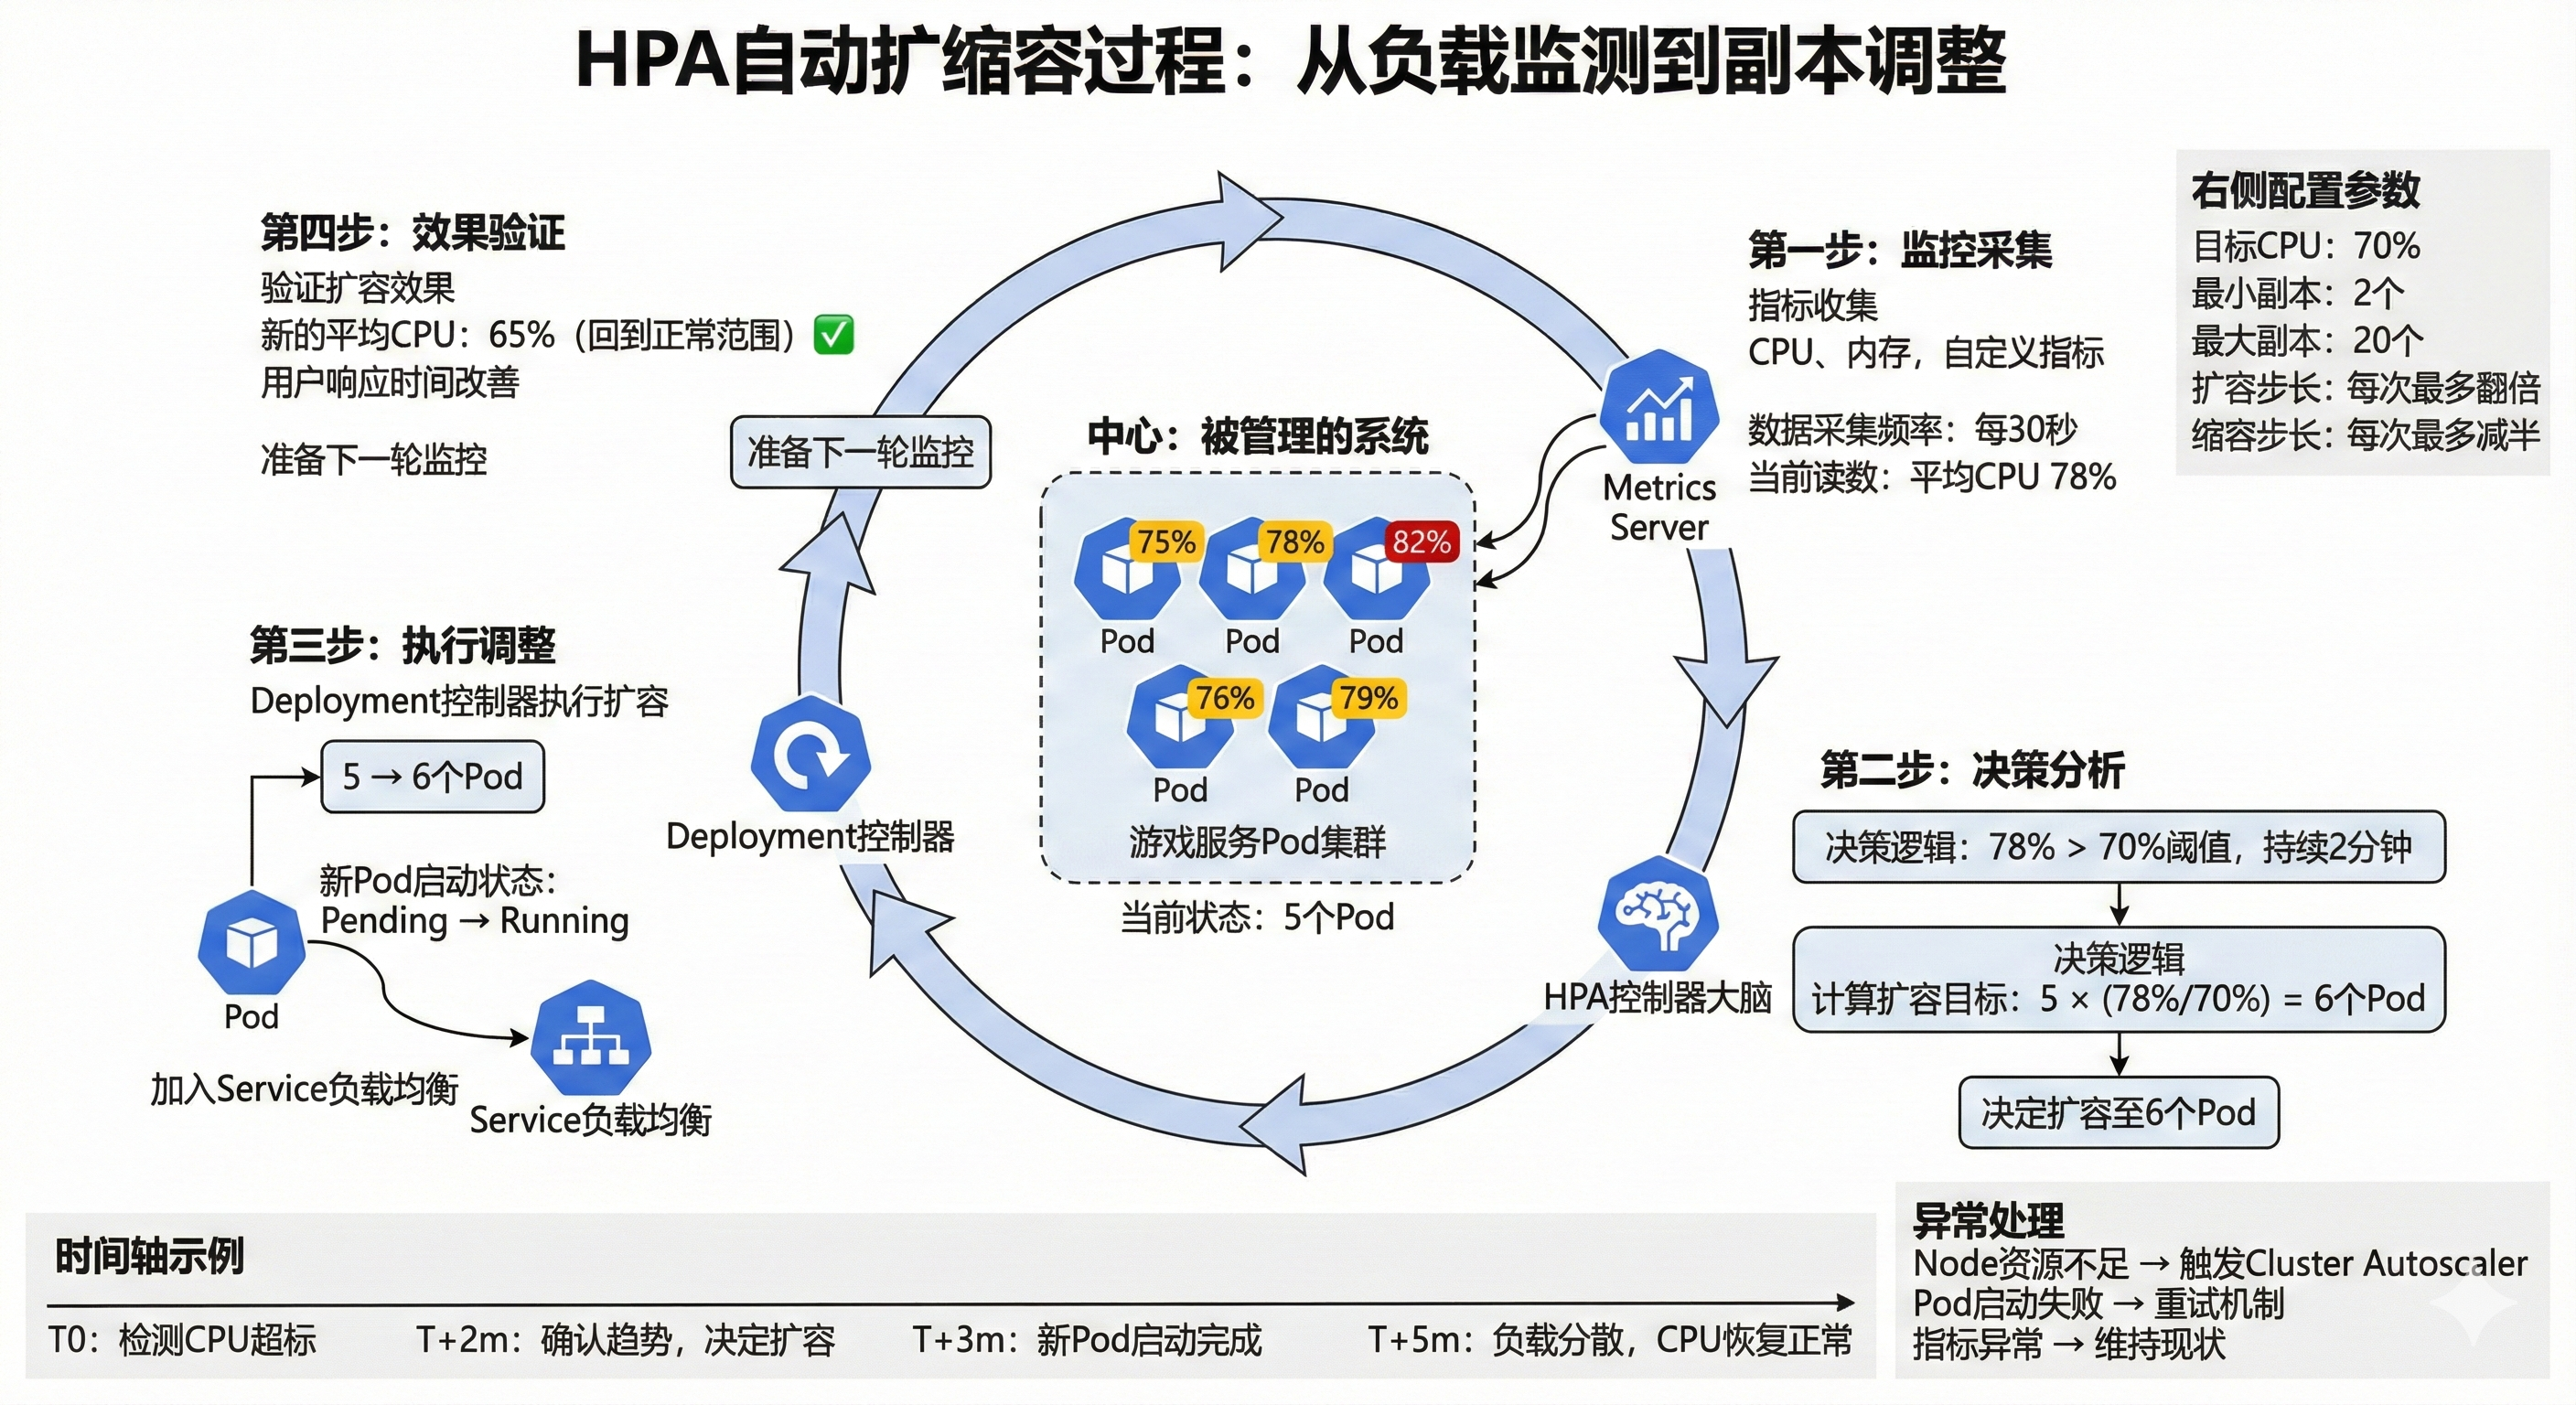
\includegraphics[width=0.9\textwidth]{figures/sec5/hpa-scaling-process.png}
\caption{HPA自动扩缩容过程：从负载监测到副本调整}
\label{fig:hpa-scaling}
\end{figure}

Horizontal Pod Autoscaler（HPA）是K8s提供的Pod级弹性方案。如图~\ref{fig:hpa-scaling}所示，HPA通过metrics server持续收集Pod的资源使用指标，当CPU使用率超过设定阈值时向Deployment发出扩容指令，负载回落时触发缩容。

从控制理论的视角看，HPA本质上是一个比例控制器（P-controller），其计算关系为：
\[
\texttt{desiredReplicas}=\lceil \texttt{currentReplicas}\times \texttt{currentMetric}/\texttt{targetMetric}\rceil
\]
例如目标CPU使用率为70\%，当前达到140\%且现有3个副本时，$\lceil 3\times 140/70\rceil=6$，扩容到6个副本。这种机制只有P项没有I项和D项，实现简单但容易出现稳态误差与振荡。为降低抖动，HPA默认设置约10\%的容忍区间，小幅偏差不触发动作，同时通过stabilization window（默认缩容5分钟、扩容0秒）防止频繁波动。

然而HPA存在固有局限。其一，端到端响应延迟：约15秒的采样周期叠加Pod启动时间，最短响应通常在45秒量级，本质上是被动响应而非提前预测。其二，热点稀释：HPA基于所有Pod的平均指标决策，如果只有个别实例因热点玩家集中而过载，平均值可能仍在阈值内，导致扩容不被触发。其三，缩容风险：对于承载活跃游戏会话的Pod，直接终止会导致玩家在对局中被强制断开。\texttt{terminationGracePeriodSeconds}为Pod预留优雅退出窗口，但这是硬超时——如果一局游戏持续20分钟而宽限期只有30秒，Pod仍会被强制终止。更务实的做法是在PreStop阶段触发"停止接收新对局"的排水状态，让当前对局自然结束，同时配合\texttt{PodDisruptionBudget}约束中断期间的最小可用副本数。

更先进的PID控制器和预测式扩缩容方案将在第六章讨论。

\subsubsection{Cluster Autoscaler：Node级扩缩}

当Pod级扩容达到Node资源的物理上限时——所有现有节点的CPU和内存都已分配完毕，新Pod处于Pending状态无法调度——就需要Node级扩容。

Cluster Autoscaler监控到Pending Pod后，分析其资源需求，请求云厂商API创建合适规格的新虚拟机实例。新Node启动并加入集群后，调度器将Pending Pod调度到新Node上运行。缩容方向上，当某个Node的利用率长期低于阈值（通常50\%），Cluster Autoscaler会评估能否将其上的Pod迁移到其他Node，如果可行则执行迁移并释放该Node。

Cluster Autoscaler还能根据Pending Pod的资源特征智能选择实例类型：CPU密集型的游戏逻辑计算选择计算优化型实例，大量缓存数据的Redis选择内存优化型实例，处理大量玩家连接的网关选择网络优化型实例。

\begin{figure}[htbp]
\centering
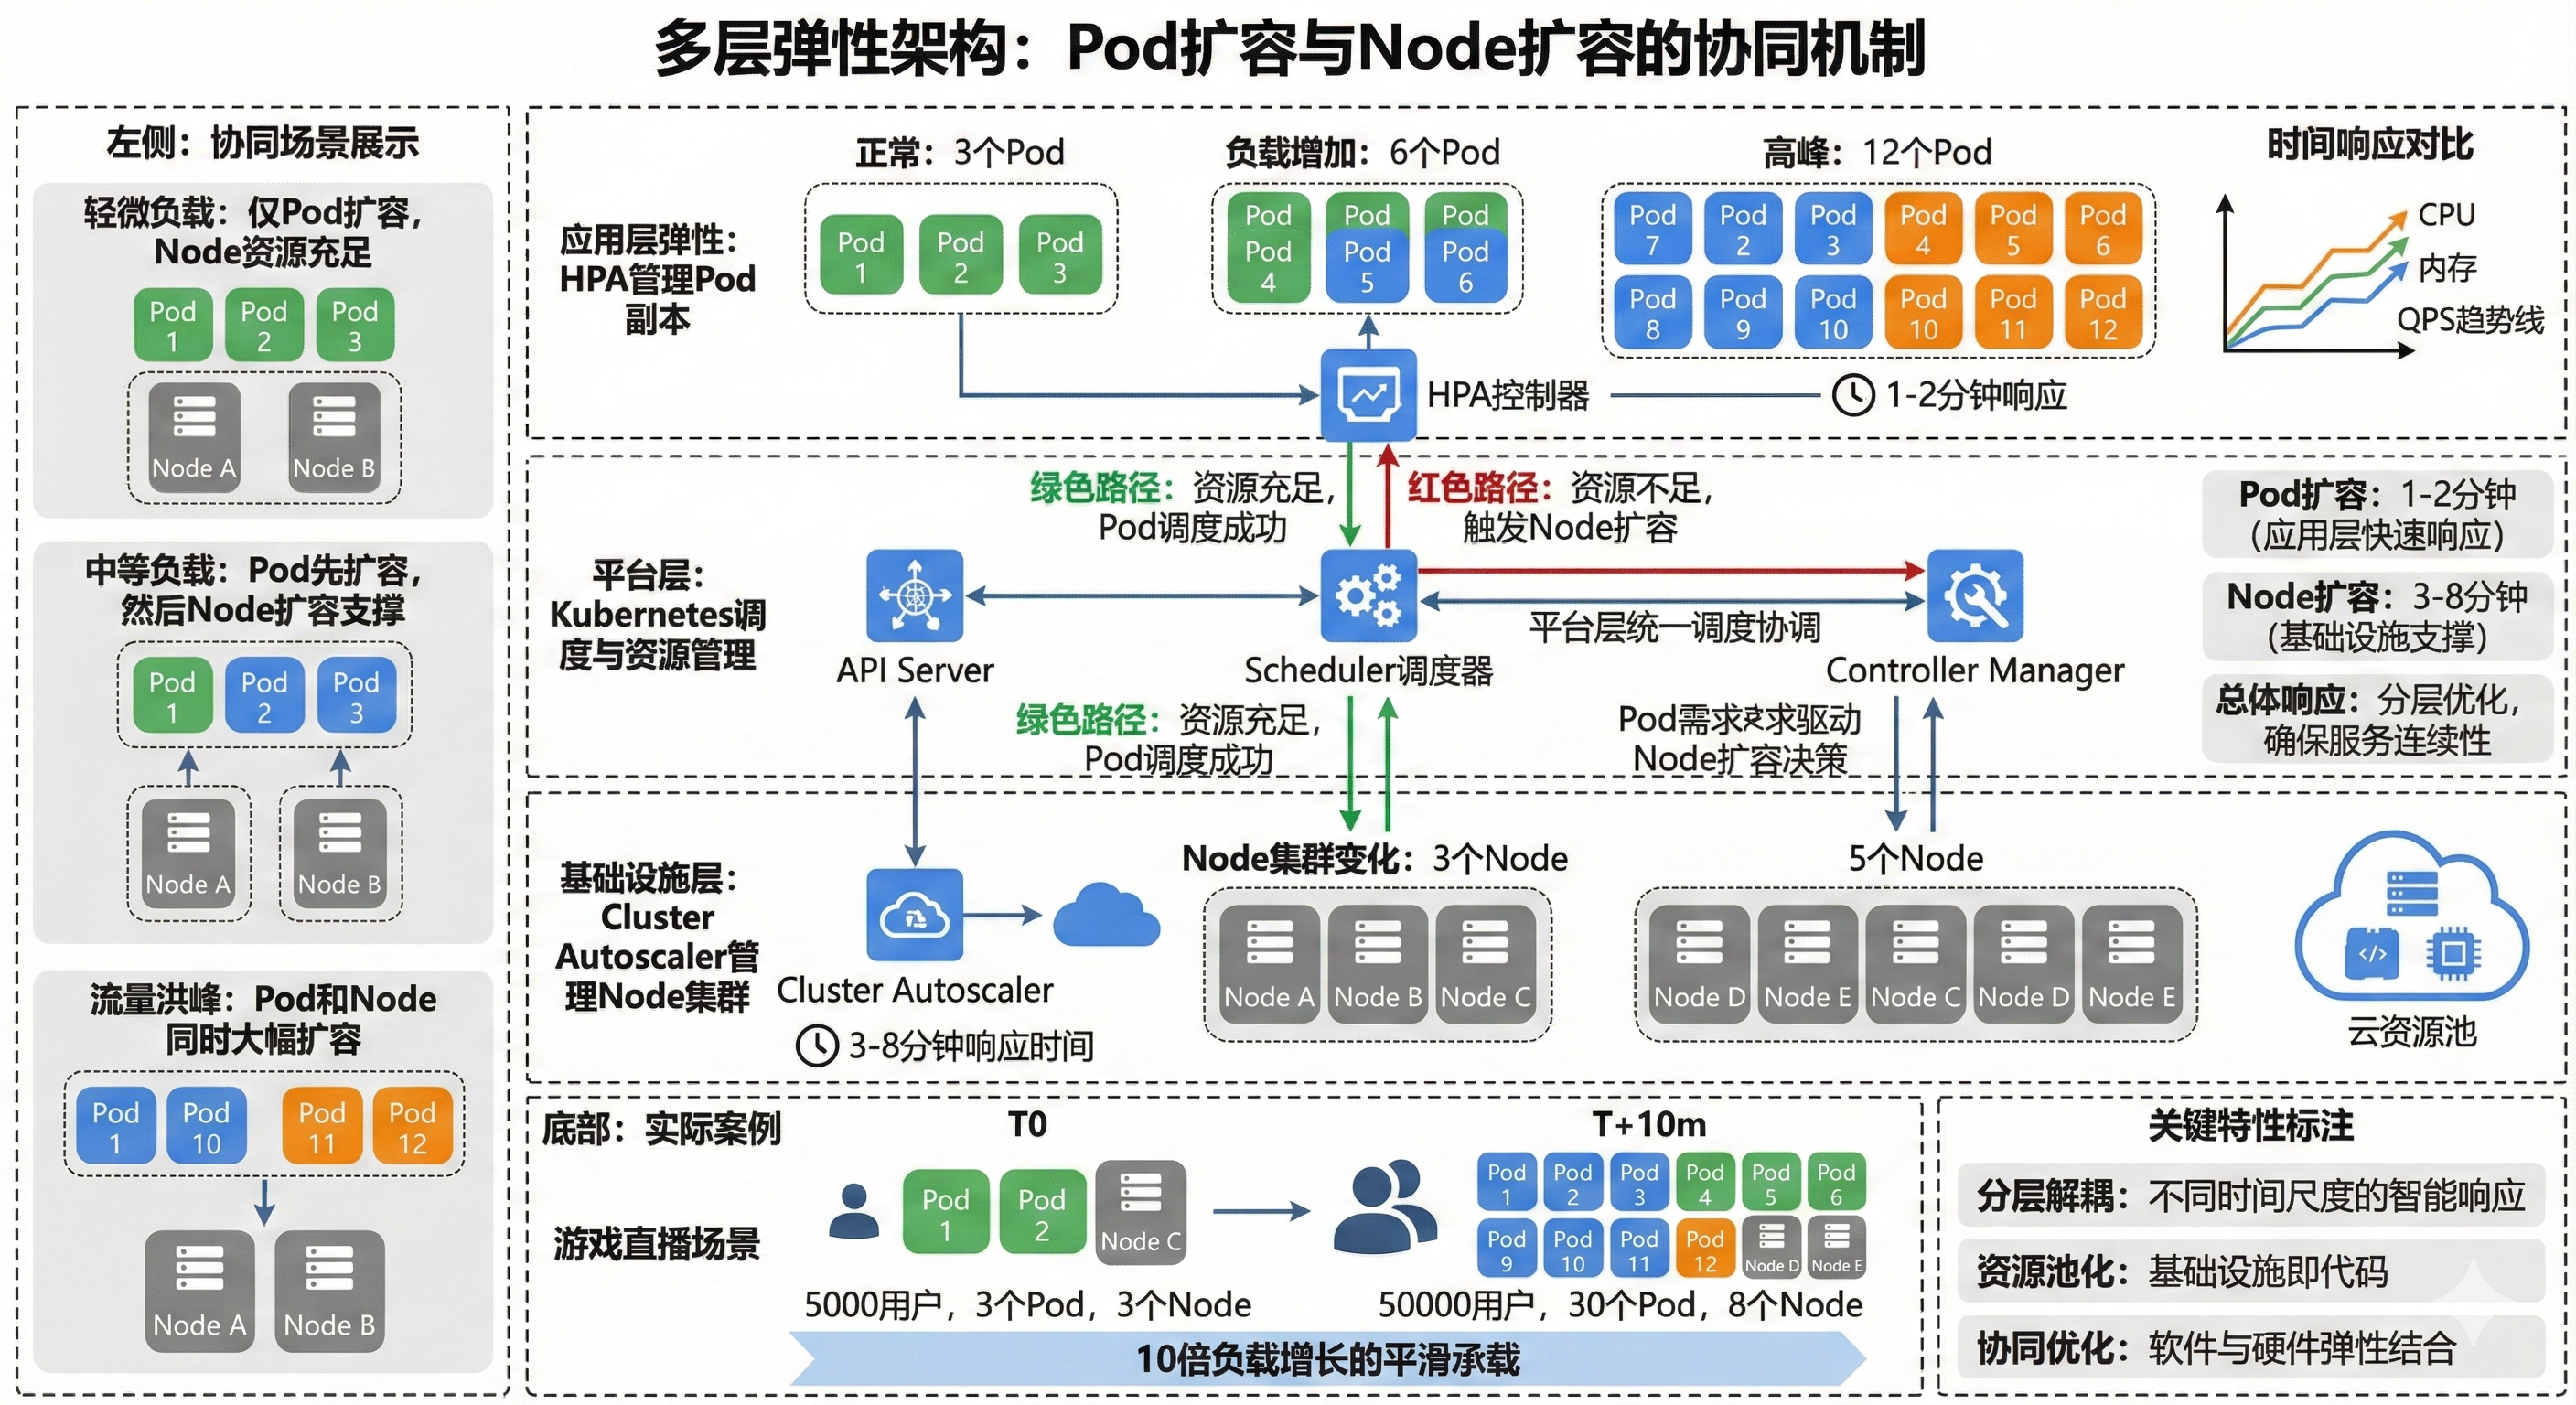
\includegraphics[width=0.9\textwidth]{figures/sec5/multi-layer-elasticity.png}
\caption{多层弹性架构：Pod扩容与Node扩容的协同}
\label{fig:multi-layer-elasticity}
\end{figure}

如图~\ref{fig:multi-layer-elasticity}所示，HPA与Cluster Autoscaler构成了两层弹性体系。HPA负责应用层的精细调度，响应速度快（1--2分钟），因为只需在现有Node上启停容器。Cluster Autoscaler负责基础设施层的宏观扩展，响应较慢（3--5分钟），因为涉及虚拟机的创建与初始化。两者配合，覆盖了从秒级到分钟级、从软件层到硬件层的弹性需求。

\subsubsection{成本经济学}

弹性扩容的价值不仅体现在技术层面，更直接反映在成本结构上。传统做法按峰值一次性采购服务器，平时常有70\%到80\%资源闲置。云上弹性按使用付费，但要做到"既省钱又稳"，关键在预留实例与按需实例的配比。

预留实例（Reserved Instance）通常比按需便宜30\%到60\%，代价是提前承诺容量与周期。按需实例（On-Demand）单价更高但调度最灵活。对游戏场景，建议把稳定底座（如长期在线的5000并发）放在预留实例上，把活动冲高部分（如从5000跃升到50000并发）交给按需实例承接。这种"基线预留加弹性按需"的策略相较纯按需常可降低40\%到60\%总云成本。竞价实例（Spot Instance）还能再便宜60\%到90\%，但可能被云厂商随时回收，适合非关键的离线批处理任务，不应承载实时对战的在线会话。

\subsection{Serverless：按调用付费的极致弹性}

\subsubsection{从K8s到Serverless：还能再省什么}

\begin{figure}[htbp]
\centering
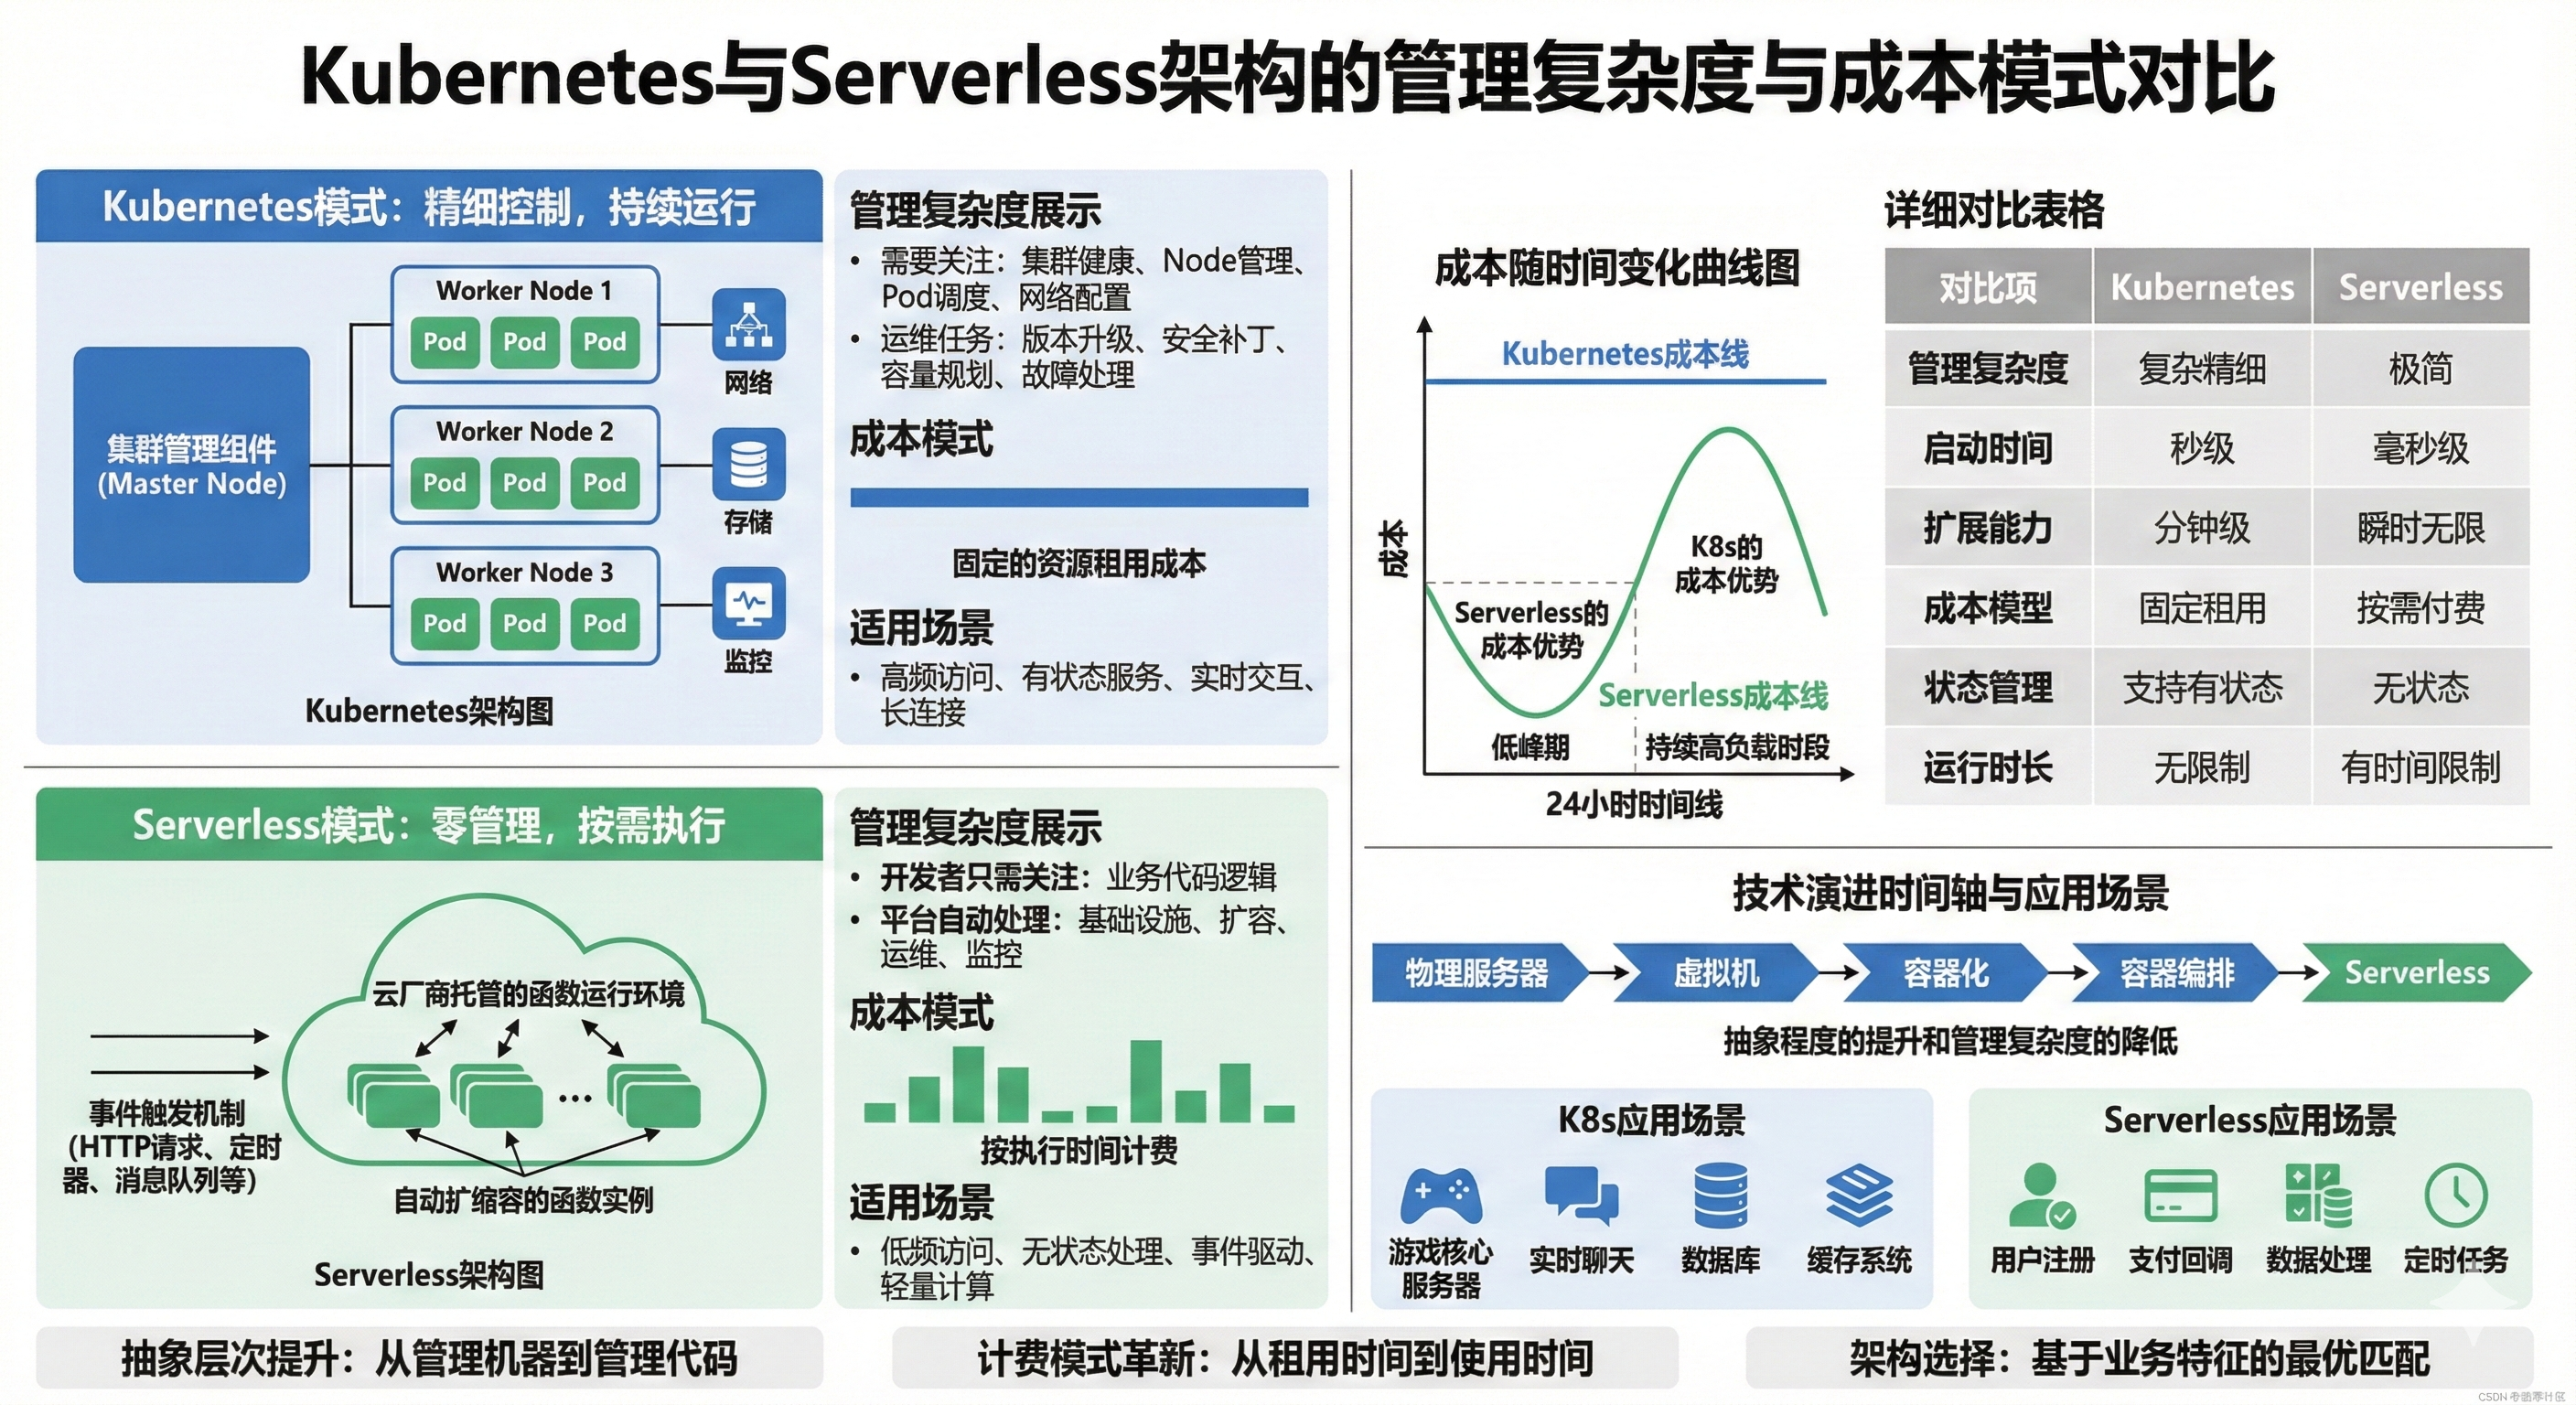
\includegraphics[width=0.9\textwidth]{figures/sec5/kubernetes-vs-serverless-comparison.png}
\caption{Kubernetes与Serverless的管理复杂度与成本模式对比}
\label{fig:k8s-vs-serverless}
\end{figure}

即使有了K8s的自动化编排和弹性伸缩，我们仍然需要关心集群的健康监控、Node的规格选择、网络安全配置等基础设施细节。对于游戏后端中那些低频、突发、轻量的辅助功能——每日签到、邮件系统、排行榜计算、活动奖励发放——专门维护一组常驻Pod显得过于沉重。

Serverless（无服务器）架构彻底抽象掉了服务器管理：你只需编写业务逻辑代码并部署到云平台，平台自动处理资源分配、弹性伸缩和故障恢复。更关键的是计费模式的变革：按代码实际运行时间收费，而非按服务器租用时间。如果没有玩家触发签到功能，代码不运行，费用为零。如图~\ref{fig:k8s-vs-serverless}所示，这种模式对具有明显波峰波谷特征的业务场景能带来显著的成本优势。

Serverless采用事件驱动的执行模型：函数按需启动，处理完请求后实例立即回收。这与K8s中Pod常驻内存、持续监听请求的模式形成鲜明对比。

\subsubsection{游戏场景的适用性分析}

\begin{table}[htbp]
\centering
\caption{Serverless与Kubernetes的场景化决策参考}
\label{tab:serverless-k8s-decision}
\begin{tabular}{|p{0.26\textwidth}|p{0.18\textwidth}|p{0.46\textwidth}|}
\hline
业务特征 & 推荐方案 & 主要原因 \\
\hline
长连接实时交互 & Kubernetes & WebSocket/TCP长连接需要稳定连接驻留，容器常驻模型更匹配 \\
\hline
有状态会话管理 & Kubernetes & 会话粘性、进程内状态与低抖动路由更容易在K8s中实现 \\
\hline
低频触发式任务 & Serverless & 按调用计费可避免空闲资源浪费，成本可下降90\%以上 \\
\hline
不可预测突发流量 & Serverless & 自动弹性能力强，能快速扩缩并减少人工容量规划压力 \\
\hline
定时批处理 & Serverless & 与事件调度天然契合，任务短平快且资源利用率高 \\
\hline
延迟敏感（$<$50\,ms） & Kubernetes & 冷启动尾延迟风险较高，常驻实例更容易保障严格时延目标 \\
\hline
\end{tabular}
\end{table}

Serverless并非适用于所有场景。如表~\ref{tab:serverless-k8s-decision}所示，核心游戏服务（实时对战、世界状态同步、聊天系统）需要维持长连接和管理复杂状态，仍然适合运行在K8s上。而周边辅助功能（用户注册、支付回调、数据分析、运营活动）通常具有无状态、低频次、可独立执行的特点，正好契合Serverless的优势。

\begin{figure}[htbp]
\centering
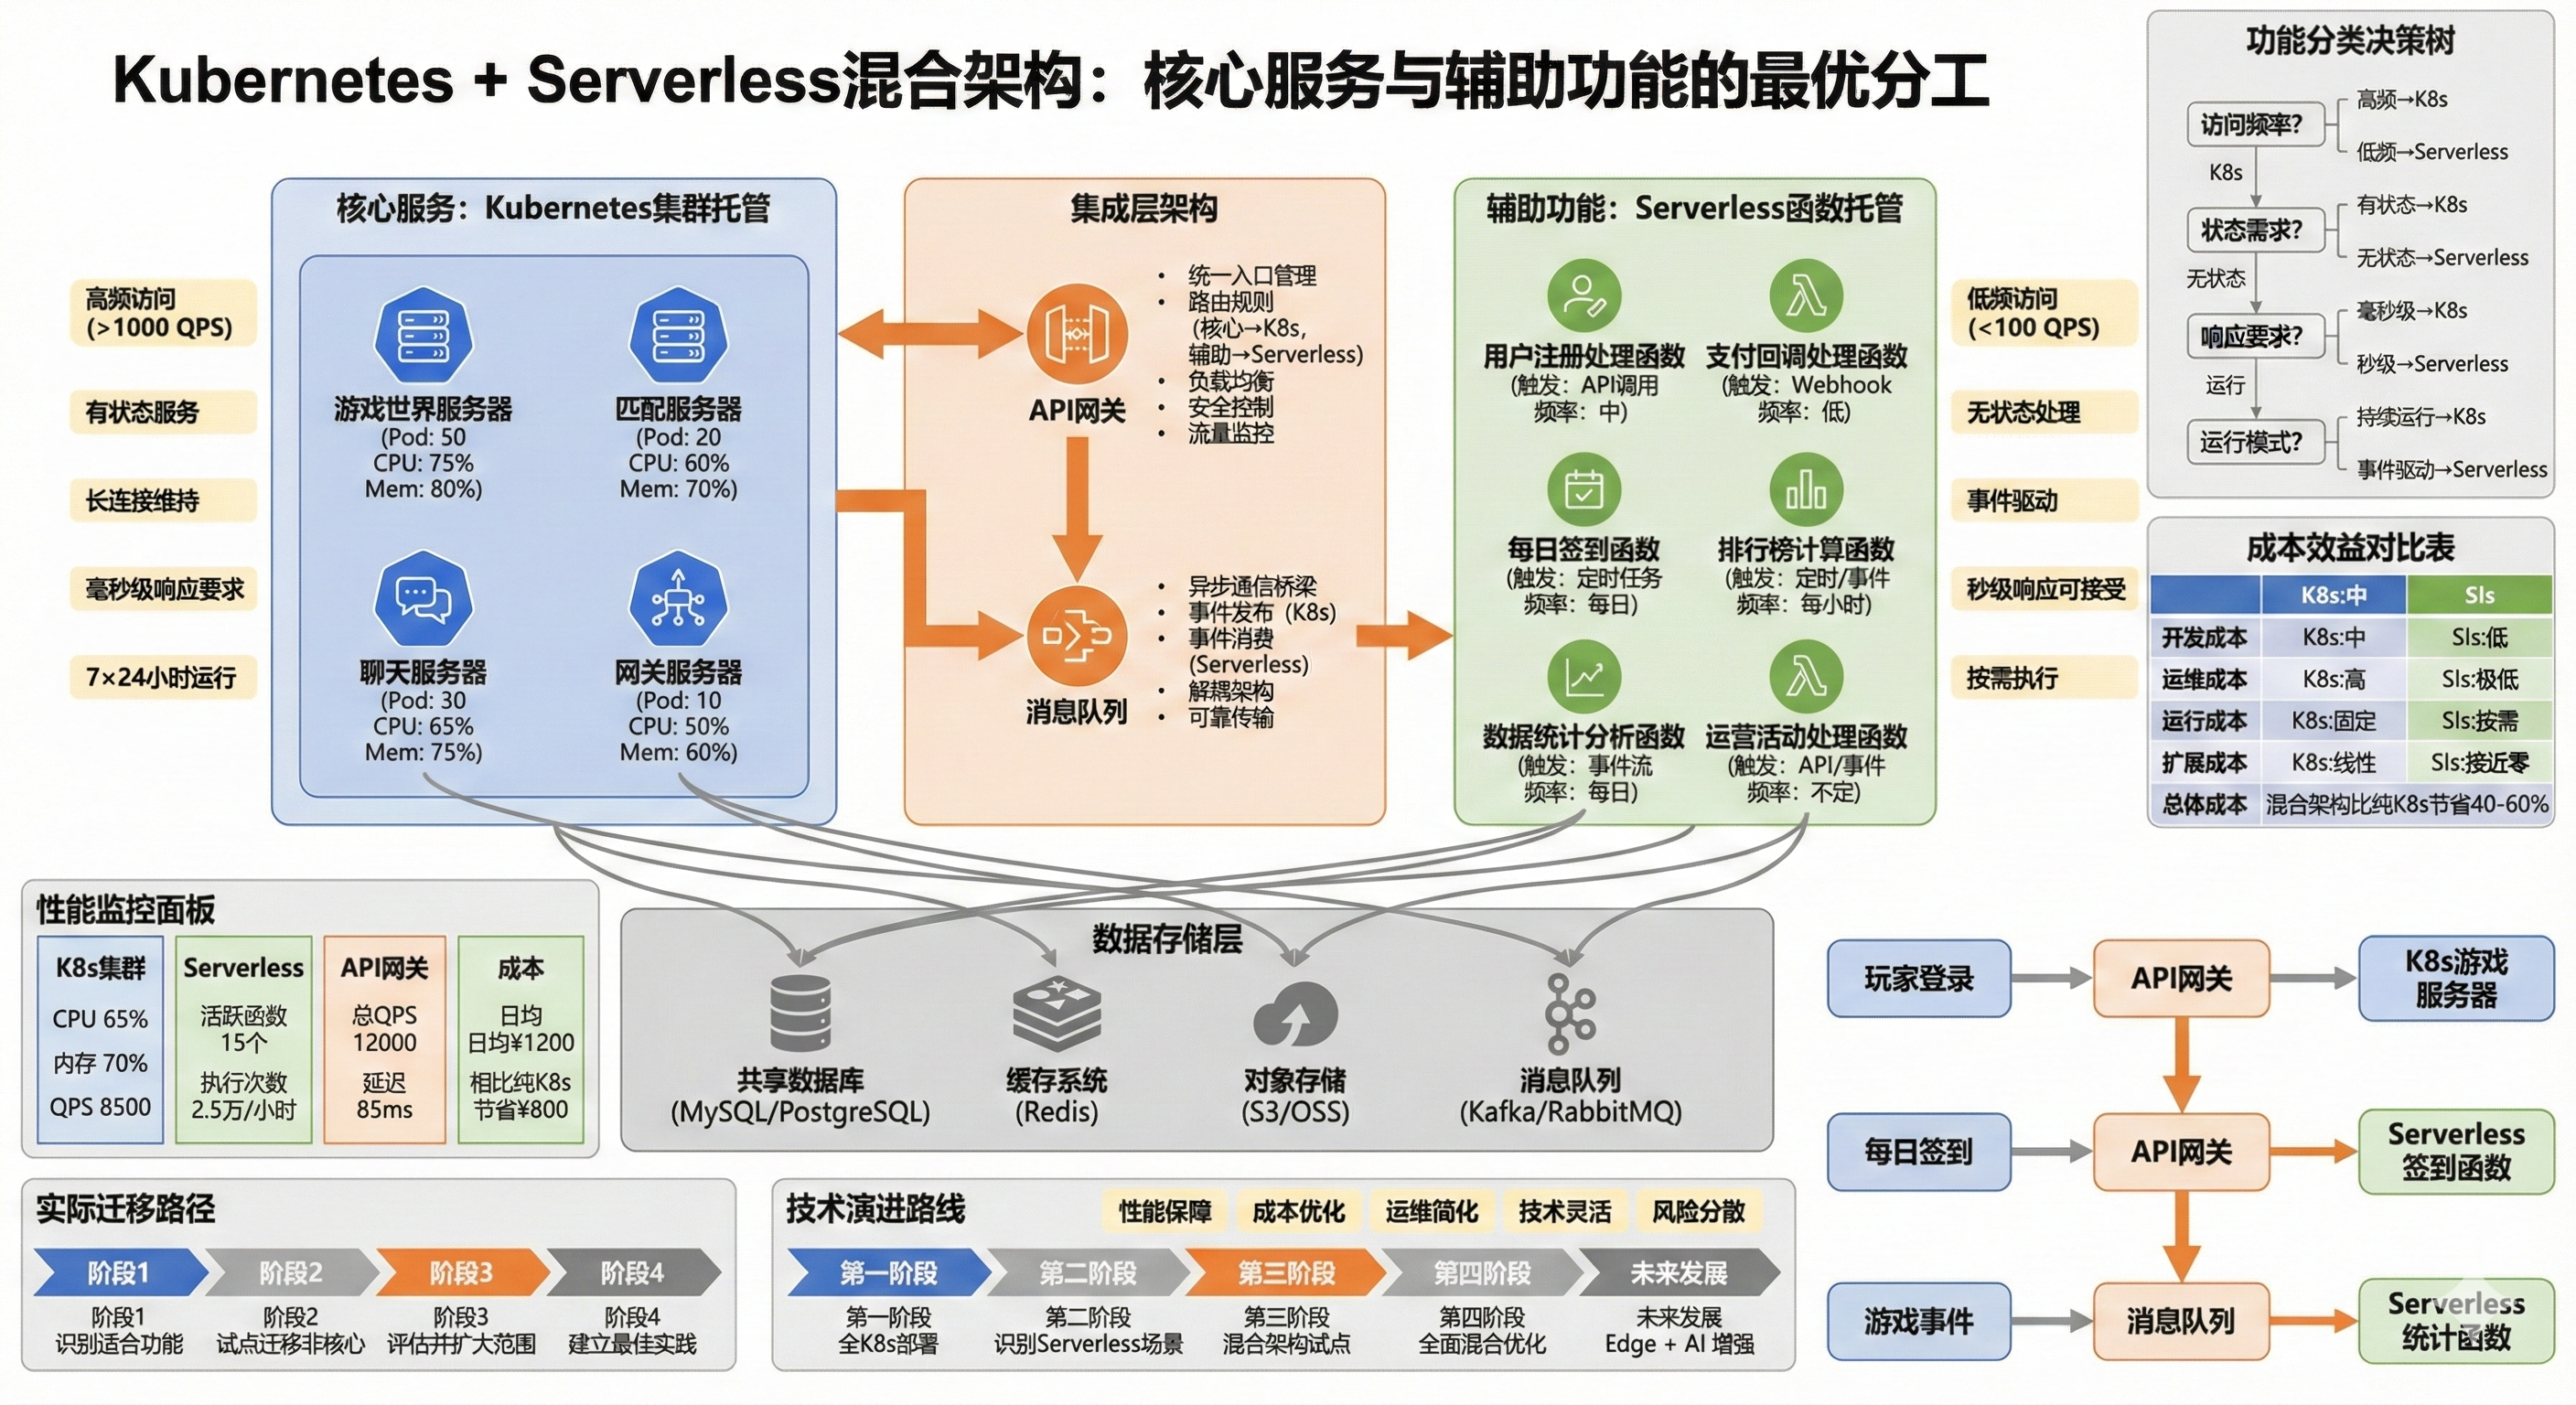
\includegraphics[width=0.9\textwidth]{figures/sec5/hybrid-architecture-design.png}
\caption{K8s + Serverless混合架构：核心服务与辅助功能的分工}
\label{fig:hybrid-architecture}
\end{figure}

如图~\ref{fig:hybrid-architecture}所示，实际项目中更常见的是混合架构：K8s集群承载核心游戏服务，Serverless函数处理辅助功能，两者通过API网关和消息队列集成。这种分层策略既保证了核心体验的稳定性，又充分利用了Serverless在成本和运维方面的优势。

\subsubsection{冷启动：Serverless的阿喀琉斯之踵}

\begin{figure}[htbp]
\centering
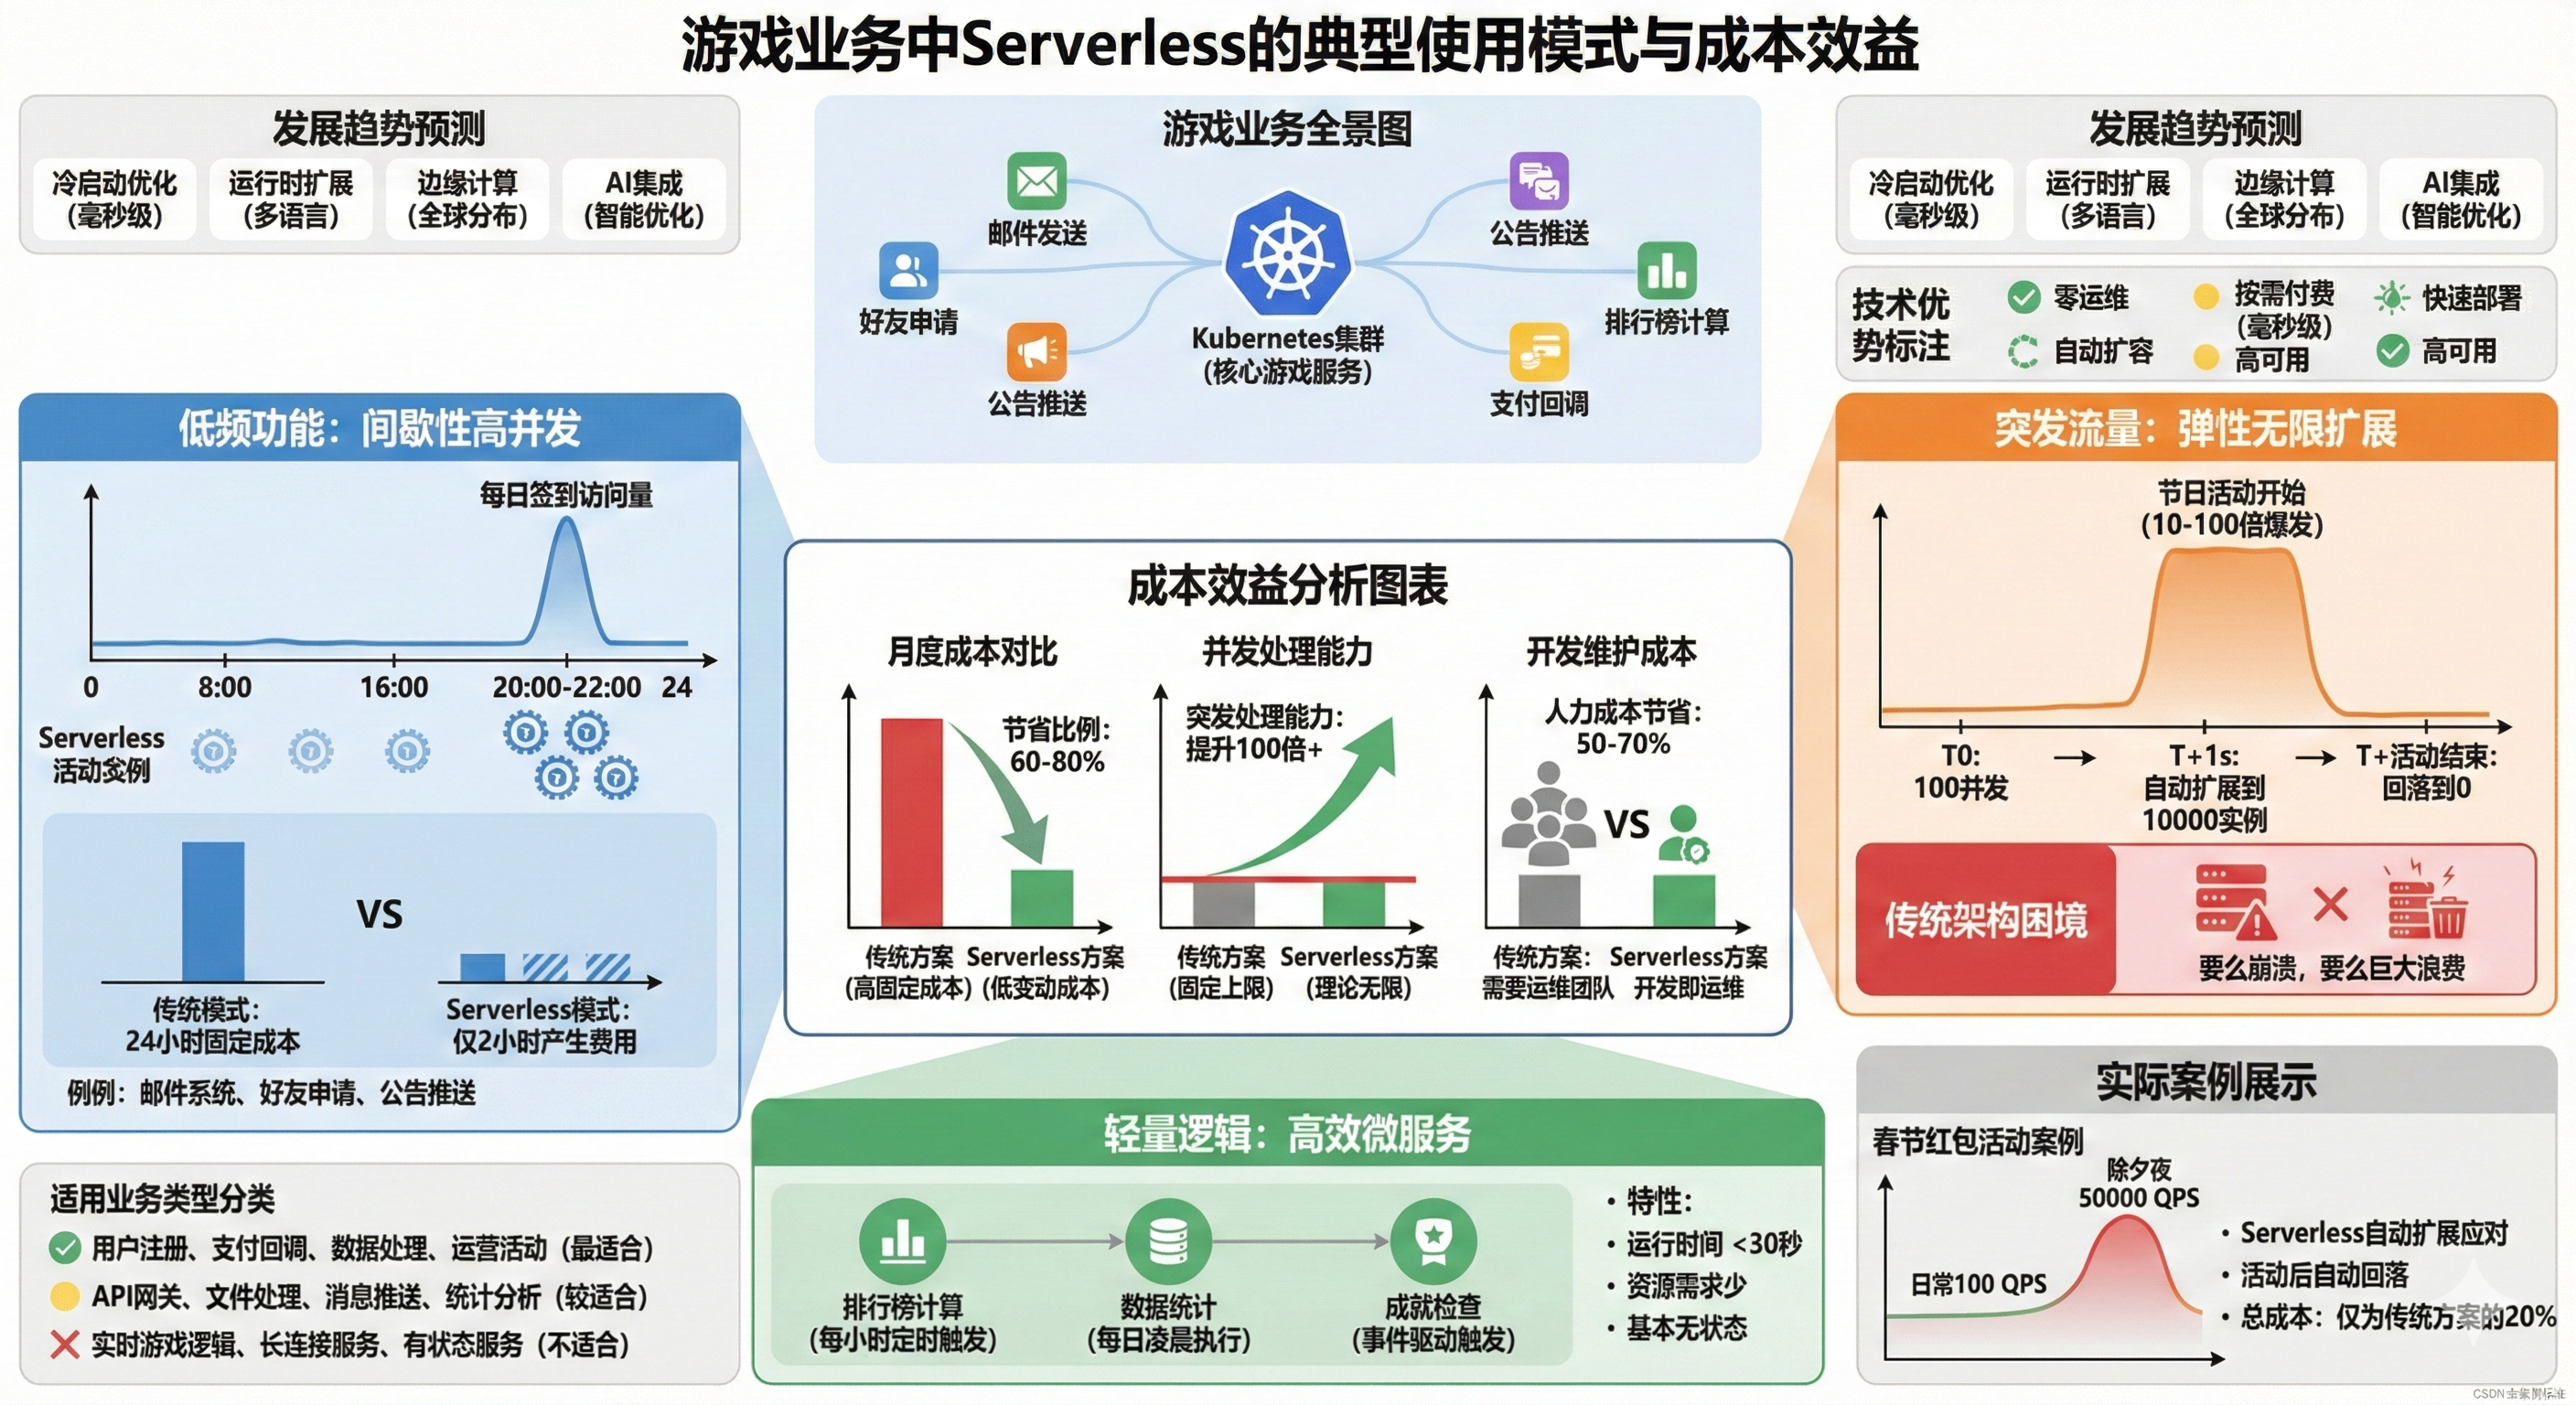
\includegraphics[width=0.9\textwidth]{figures/sec5/serverless-usage-patterns.png}
\caption{Serverless的典型使用模式与冷启动影响}
\label{fig:serverless-patterns}
\end{figure}

Serverless最被诟病的问题是冷启动延迟。当一个函数实例不存在时，平台需要从零创建执行环境，这个过程由多个串行阶段叠加而成。

第一阶段是执行环境创建：平台完成沙箱分配、网络与文件系统挂载等基础准备。在主流实现中，Firecracker microVM的启动时间约125\,ms，同时保持接近虚拟机级别的隔离性。第二阶段是运行时初始化：不同语言差异显著——Go与Rust的启动开销接近零，Python和Node.js增加几十到数百毫秒，传统JVM在类加载和JIT预热场景下可能增加秒级延迟。第三阶段是应用代码加载：依赖导入、数据库连接建立、配置读取等，这部分最受开发者控制。

工程上的优化重点应放在可控环节：对稳定高峰流量使用预留并发（Provisioned Concurrency）进行预热（但会增加常驻成本）；优先选择轻量运行时；JVM场景考虑GraalVM Native Image缩短启动路径；缩小部署包体积、减少无关依赖，并通过延迟加载将非首请求必需的逻辑后置。关于快照恢复（snapshot-restore）如何进一步压缩甚至消除冷启动，以及gVisor、Kata Containers等轻量虚拟化方案的原理对比，我们将在第六章展开。

\subsection{小结：从手工作坊到云原生工业}

本章的旅程，是一场被问题驱动的逐步演进。

起点是一个具体的工程困境：第四章设计好的分布式游戏后端，要部署到真实的云服务器上运行。我们首先遭遇了环境一致性问题——同一份代码换台机器就跑不了。比较了手工安装、虚拟机和容器三条路径后，我们选择了Docker：用镜像封装完整的运行环境，用分层构建实现高效复用，用Registry和摘要锁定实现可靠分发。

单个容器的问题解决后，多容器的协同启动成为新的痛点。Docker Compose通过声明式配置将手工操作收敛为一条命令，但它的能力边界止于单机。当我们需要跨多台机器调度容器、自动故障恢复和滚动更新时，Kubernetes接管了编排职责。K8s的核心价值在于声明式管理和持续调谐：你描述期望状态，系统自动逼近并维持。

有了集群编排能力后，"固定配置遇上波动流量"的成本矛盾浮出水面。HPA和Cluster Autoscaler构成的两层弹性体系，让资源能够跟着负载自动伸缩。而对于低频、突发、轻量的辅助功能，Serverless提供了按调用付费的极致弹性，与K8s形成互补的混合架构。

每一步都是被前一步的局限性逼出来的：环境不一致逼出了容器，多容器管理逼出了Compose，单机局限逼出了K8s，成本矛盾逼出了弹性伸缩，运维负担逼出了Serverless。这条演进路径不是人为设计的技术堆叠，而是工程实践中自然生长出来的解决方案链。

至此，我们的游戏架构已经从一个脆弱的本地原型，进化为一套能够根据流量自动伸缩、故障自动恢复的云原生系统。但我们目前掌握的是"驾驶"这辆云原生战车的能力——会用Docker封装、会用K8s编排、会配置弹性策略。当匹配服在晚高峰抖动、战斗服时延突增、灰度发布引发连锁故障时，只有理解系统内部的机理，才能做出稳定的技术判断。下一章，我们将真正打开引擎盖，深入容器隔离、调度算法、控制论、服务网格等底层原理。

\newpage
\section{第六章\ 屠龙之术：云原生核心原理}

在第五章中，我们学会了驾驶云原生这辆战车：用Docker把游戏服务装进容器，用Kubernetes编排和管理容器集群，用HPA让Pod数量跟着负载自动伸缩，还体验了Serverless的按需执行模式。这些工具确实强大，但如果你只会用它们，遇到问题时就只能对着黑盒干瞪眼——战斗服突然卡顿，你不知道是容器隔离出了问题还是网络虚拟化的开销；HPA扩容太慢导致玩家排队，你不知道该调哪个参数；Serverless冷启动让签到功能首次响应很慢，你不知道瓶颈在哪个阶段。

本章的目标，是打开这些工具的引擎盖，搞清楚里面的零件是怎么运转的。我们会沿着四个问题逐步深入：容器的隔离是怎么实现的？容器之间的网络是怎么搭建的？HPA这样的自动扩缩容控制器是怎么写出来的？Serverless引擎是怎么做到毫秒级启动一个执行环境的？前两个问题是地基——没有隔离和网络，容器就无从谈起；后两个问题是上层建筑——弹性伸缩和Serverless是云原生最核心的能力，也是最难实现的部分。

如果说前四章是教你从零手写一个游戏服务引擎，第五章是教你怎么用现成的云原生工具部署它，那么本章就是教你：如果这些工具不存在，你能不能自己造出来？

\subsection{容器的本质：操作系统级虚拟化的三块基石}

本节讨论的“容器”，指的是 Linux 上的\textbf{操作系统级虚拟化}。它与虚拟机的思路不同：虚拟机在硬件之上再“虚拟出一台机器”，因此每个虚拟机通常有自己的内核；而容器不模拟硬件，它让多个应用进程\textbf{共享同一个宿主机内核}，但每一组进程都像“生活在自己的小世界里”。从结果看，容器也能做到“互不干扰”，但它依赖的不是虚拟硬件，而是内核提供的三类机制：\textbf{Namespaces} 用来隔离“看见什么”，\textbf{Cgroups} 用来限制“能用多少”，\textbf{OverlayFS/rootfs} 用来构造“看到的文件系统长什么样”。

为了让读者从直觉走到机制，本节不从工具（Docker）出发，而从一个最简单的问题出发：为什么在宿主机上执行 \texttt{ps aux} 能看到很多进程，而在容器里执行同样的命令，往往只看到容器自己的那几个进程？回答这个问题，就需要先把 Namespace 讲清楚。 % 图

\subsubsection{Namespaces：让进程拥有“独立的系统视图”}

在没有隔离机制时，Linux 系统中的许多关键资源在逻辑上是“全局共享”的。例如，系统只有一套进程号的编号规则，只有一棵统一的挂载目录树，只有一套网络协议栈，也只有一个主机名。进程之所以能“看见”这些资源，是因为它通过系统调用向内核查询或操作这些全局对象：例如 \texttt{getpid()} 返回进程号，\texttt{hostname} 查询主机名，\texttt{mount} 查询挂载信息，\texttt{ip addr} 查询网络接口等。由于这些对象在默认情况下是全局的，所以任何进程看到的结果基本一致。

\textbf{Namespace（命名空间）}是 Linux 内核提供的一种隔离机制，它的思想可以用一句通俗的话概括：\textbf{同一类系统资源不再只有“全局唯一的一份”，而是可以被划分成多份；每个进程只属于其中一份，因此它只能看见那一份资源。}这意味着 Namespace 做的不是“隐藏”，而是\textbf{把“全局对象”变成“按组划分的对象”}，从而让不同进程组拥有不同的系统视图。

容器常用的几类 Namespace 分别隔离不同维度的视图。PID Namespace 隔离进程号空间；Mount Namespace 隔离挂载树；Network Namespace 隔离网络栈；UTS Namespace 隔离主机名。它们叠加在一起，就形成了容器最直观的效果：容器内运行 \texttt{ps} 时只看到容器自己的进程；容器内查看网络接口时，只看到属于容器的接口（最初往往只有回环接口 \texttt{lo}）；容器内的主机名可以与宿主机不同；容器内的目录结构也可以与宿主机不同。

需要特别强调的一点是：Namespace 并不是在用户态“改写命令输出”。例如，容器内执行 \texttt{ps} 看不到宿主机进程，并不是 \texttt{ps} 被修改了，而是因为 \texttt{ps} 读取的是 \texttt{/proc} 中的进程信息；在 PID Namespace 生效后，内核只会把该命名空间中的进程暴露到 \texttt{/proc} 的视图里，因此 \texttt{ps} 自然“只能看到那么多”。同理，\texttt{ip addr} 显示的网络接口来自内核网络子系统；Network Namespace 生效后，该命名空间拥有独立的网络接口集合，命令读到的也就只剩下容器自己的那一份。这一点非常重要：\textbf{隔离发生在内核层，用户态工具只是如实读取内核提供的视图。}

从“如何创建”角度看，Namespace 不是某种额外软件，而是内核为进程提供的一个属性。创建新 Namespace 的常见方式有两类。第一类是在创建子进程时显式要求进入新的命名空间，典型接口是 \texttt{clone} 系统调用（在 Go 中体现为设置 \texttt{Cloneflags}）。第二类是让当前进程主动切换到新的命名空间，典型接口是 \texttt{unshare} 系统调用。无论哪一种方式，本质效果相同：\textbf{内核把进程加入到某个命名空间实例中，并从此按该实例的规则向进程呈现系统资源。}

理解 PID Namespace 时，有一个教学上最容易忽略、但对理解非常关键的事实：\textbf{容器内的第一个进程在该 PID Namespace 中是 PID 1。}在 Linux 中，PID 1 的语义比较特殊，它承担了“回收僵尸进程”和“信号处理的特殊规则”等职责。因此，容器运行时往往会在容器内部引入一个极小的“init 进程”（例如 \texttt{tini}），以保证容器内进程退出与信号转发行为符合预期。这里的重点不是记住某个工具名，而是理解：\textbf{PID Namespace 会让容器内部重新出现一个“从 1 开始的进程世界”，因此容器内部也需要有人扮演 PID 1 的角色。}

到这里，读者应该可以用一句话把 Namespace 的作用说清楚：\textbf{Namespace 把原本全局共享的系统资源按组切分，并为进程提供一套“只属于它那一组”的系统视图。}有了这层视图隔离，容器才具备“看起来像一台独立机器”的第一步。

\subsubsection{Cgroups：把资源使用变成“可计量、可限额、可统计”的对象}

如果说 Namespace 解决的是“容器看见什么”，那么 Cgroups 解决的就是“容器最多能用多少”。仅靠视图隔离并不能避免资源争用：某个容器即使看不见其他容器的进程，也仍然可以把 CPU 长时间跑满，或者把内存一路申请到系统紧张，最终拖慢整台机器上的所有服务。因此，一个真正可用的容器体系必须提供\textbf{资源控制}，让每个容器的资源使用在可预期范围内。

Linux 的 \textbf{Cgroups（Control Groups，控制组）}可以用一个非常直观的比喻来理解：\textbf{Namespace 像“房间的门牌号与视野”，而 Cgroups 像“水电表与限额器”。}Cgroups 的基本思想是先把一批相关进程归为一个组，然后由内核对这个组的资源使用进行管理。这里的“管理”主要包含两层含义：一是\textbf{限制}，例如这个组最多可以使用多少 CPU、最多占用多少内存；二是\textbf{统计}，例如实际使用了多少、是否因为超额而被限速、是否触发了内存回收。容器运行时并不会让应用进程自觉地节制资源，而是把规则交给内核，由调度器和内存管理器强制执行。

理解 Cgroups 时，最重要的不是记住某个命令或文件名，而是把握它与调度器之间的关系。以 CPU 为例，操作系统调度线程运行时，本质上是在决定“谁在什么时候可以占用 CPU”。Cgroups 在这里插入了一个简单但非常有效的约束：\textbf{对某个进程组规定一个时间预算，在固定的时间窗口内，这个组最多只能运行这么久。}可以把它理解为“周期性发放的 CPU 额度”。每到一个新周期开始，内核就给该控制组发放一定的 CPU 时间预算；组内所有线程在运行时共同消耗这份预算；一旦预算被消耗完，控制组内的线程就会被暂停，直到下一个周期再次发放预算才恢复运行。由此可见，CPU 限制并不是“固定分配某个核心”，而是“限制一段时间里累计可运行的总时长”。

这一点会带来一个初学者很容易误解的现象：\textbf{同样的配额，在单线程与多线程场景下表现会完全不同。}原因是预算按控制组整体计算，而不是按线程计算。多个线程并行时，预算消耗速度会显著加快：如果同时有 $k$ 个线程在不同核心上并行运行，那么预算的消耗速度近似是单线程的 $k$ 倍。于是就可能出现这样一种看似“反直觉”的情况：宿主机还有空闲 CPU 核心，但某个容器却突然“整体卡住”。从内核角度看，这并不反直觉，因为该容器所属的控制组在当前周期内已经把预算用完，必须等待下一个周期“重新发放额度”。

同样的思想也适用于内存控制。内存限制的含义不是“建议你少用点”，而是\textbf{为进程组规定一个可使用的上限}。当容器内进程持续申请内存并逼近上限时，内核会更积极地回收页面、触发内存压力；如果仍然超出上限，就可能触发 OOM（Out Of Memory）策略，对容器内进程进行终止，以避免系统整体失稳。也就是说，内存限制的目标是把“局部失效”留在容器内部，而不是让“全局崩溃”扩散到整台机器。

因此，读者可以用一句话概括 Cgroups 的作用：\textbf{Cgroups 把“资源使用”从单个进程的行为，上升为内核可管理的进程组属性；它让资源的使用变得可计量、可限额、可统计，从而保证多容器并存时的可预期性与稳定性。}理解了这一点，Docker/Kubernetes 中的 CPU limit、memory limit 等配置就不再是“工具参数”，而是内核机制的直接映射。


\subsubsection{rootfs 与 OverlayFS：为什么镜像能分层，容器又为什么能写}

前面两部分解释了容器的“视图隔离”（Namespace）与“资源限额”（Cgroups）。但如果容器只是隔离进程和资源，而没有一套独立的文件系统，那么容器内的程序仍然会直接读写宿主机的目录树，这显然不符合“像一台独立环境”的直觉。因此，容器还必须回答第三个问题：\textbf{容器里看到的文件系统从哪里来？多个容器能否共享同一份基础环境？容器运行时产生的文件又存到哪里？}

理解这一点，需要先把 \textbf{rootfs} 讲清楚。对 Linux 进程而言，所有路径（例如 \texttt{/bin/sh}、\texttt{/etc/hosts}）都是相对于“根目录 \texttt{/}”展开的。所谓容器的 \textbf{root filesystem（rootfs）}，就是：\textbf{让容器内进程把某个目录当作自己的根目录 \texttt{/}}。当 rootfs 指向一份精心准备的目录树时，容器内的程序就会以为自己运行在一套独立的系统环境里：\texttt{/bin} 里有可执行文件，\texttt{/lib} 里有动态库，\texttt{/etc} 里有配置文件。容器镜像实际上就是在为 rootfs 提供内容：它提供一份可以作为根目录的文件系统快照。

接下来是“分层”的问题。镜像之所以要分层，是因为大量容器往往共享相同的基础环境：同一个 Linux 发行版、同一套运行时库、同一套依赖包。如果每启动一个容器都复制一份完整目录树，磁盘空间与启动时间都会被浪费。更理想的做法是：\textbf{基础环境只保存一份并且只读共享，每个容器只保存自己的改动。}Linux 的 \textbf{OverlayFS（叠加文件系统）}正是用来实现这种“只读基座 + 可写薄层”的机制。

OverlayFS 可以用一个非常直观的类比来理解。把镜像的基础文件系统想成一本印刷好的教材（只读、可复用）；把容器运行时的写入想成在教材上做笔记。我们当然不希望每个学生都去重新印一本教材，也不希望在教材原件上直接涂改。更合理的方式是：每个学生在教材上铺一张透明的塑料膜，把笔记写在膜上。阅读时看起来像是“教材被修改了”，但实际上原教材完全不变，笔记只存在于各自的膜上。OverlayFS 的工作方式与此几乎一致。

更具体地说，OverlayFS 把两层目录合成一个统一视图：\textbf{下层是只读的基础层（镜像层），上层是每个容器独有的可写层（容器层）。}容器内的进程访问文件时，并不是分别去“读基础层还是读容器层”，它看到的是合并后的结果：同一个路径在合并视图中只有一份。但内核在背后遵循一条简单规则：\textbf{读的时候优先从可写层找，找不到再去只读层；写的时候永远写入可写层。}这条规则直接带来两个关键效果。

第一，\textbf{共享变得容易}。因为基础层是只读的，它可以被很多容器同时使用而不会相互影响。无论启动多少个容器，基础层都只需要在磁盘上保存一份，这就是镜像分层能够节省空间的根本原因。

第二，\textbf{写入不会破坏基础层}。当容器创建一个新文件时，这个文件只会出现在该容器的可写层里；基础层不会改变。当容器修改一个原本只存在于基础层的文件时，也不会直接改动基础层。内核会先把该文件从只读层“复制”到可写层，然后在可写层修改副本。这种策略称为\textbf{写时复制（copy-on-write）}：只有当确实发生写入时才复制，因此既避免了全量复制的成本，也保证了基础层的共享与不变。

有了这一机制，很多容器现象就可以用统一语言解释。比如，“删除容器后数据丢失”并不是因为镜像坏了，而是因为容器运行时的改动主要保存在它自己的可写层；当容器被删除时，可写层随之清理，而只读的镜像层仍然存在，因此“环境还在，数据没了”。同样，如果希望数据不随容器消失，就需要把数据放到不属于可写层的地方（例如挂载宿主机目录或使用独立卷），这就是容器持久化存储的动机。

总结来说，\textbf{rootfs} 解决的是“容器把哪一份目录树当作 \texttt{/}”；\textbf{OverlayFS} 解决的是“这份目录树如何既能共享基础环境，又能允许每个容器独立写入”。理解了这两点，就能把“镜像分层”“容器可写”“删除容器数据消失”等现象从机制层面串成一个闭环。

从工程视角看，这也正是容器解决“依赖环境复杂”的关键。游戏服务往往同时依赖特定版本的运行时与系统库：例如某个组件需要特定版本的 \texttt{glibc/libstdc++}，另一个组件依赖某套语言运行时与第三方包；如果这些依赖直接安装在宿主机上，就很容易出现版本漂移与相互污染，最终变成“这台机器能跑、那台机器跑不起来”。镜像提供的 rootfs 本质上就是一份可复制的依赖闭包：可执行文件、动态库、配置目录都被放进同一份目录树里，容器启动时再通过挂载把它变成进程看到的根目录 \texttt{/}，从而让进程读取到的 \texttt{/bin}、\texttt{/lib}、\texttt{/usr} 与宿主机解耦。

镜像分层与 OverlayFS 进一步把依赖环境的复用与隔离同时做到：基础层可以被多个服务共享（同一发行版与通用运行时只保存一份），服务层只叠加该服务独有的依赖与二进制；运行时写入则落在容器自己的可写层里，不会回写到基础层，也不会污染其他容器。这样，调度器把同一个镜像放到任何节点上启动出来，依赖环境都一致；而 Cgroups 使得不同依赖栈的进程组在同机共存时仍能被限额与统计，避免某个服务的资源峰值拖慢整机。

\subsubsection{容器的安全边界：为什么容器不等于“更轻的虚拟机”}

理解了 Namespaces、Cgroups 与 OverlayFS 之后，我们已经可以解释容器的大部分“表面现象”：它看起来像一台独立机器，有自己的进程列表、网络接口与目录结构，并且资源使用还能被限制。但在安全边界上，容器与虚拟机仍然存在本质差异。虚拟机的隔离来自\textbf{硬件虚拟化与 Hypervisor}：每个虚拟机通常运行自己的内核，内核之间由虚拟化层隔开。容器则不同：\textbf{所有容器共享同一个宿主机内核}。因此，容器的隔离更准确地说是“同一内核中的隔离”，而不是“不同内核之间的隔离”。

这一区别带来的直接后果是：Namespace 与 Cgroups 虽然能让容器“像是独立的”，但它们并不自动提供与虚拟机同等级别的安全边界。Namespace 主要改变的是\textbf{进程看到的系统视图}，例如看见哪些进程、哪些网络接口、哪些挂载点；Cgroups 主要控制的是\textbf{资源使用额度}，例如最多能用多少 CPU 时间、最多能占用多少内存。它们都不改变一个事实：容器内的进程执行系统调用时，最终仍然进入\textbf{同一个宿主机内核}。因此，一旦内核存在可被利用的漏洞，攻击者就可能借助漏洞突破隔离边界，从容器影响宿主机，这就是所谓“容器逃逸”的根源。

在解释前面提出的“\texttt{ps aux} 为什么不一样”的问题时，正好可以把“视图隔离”与“共享内核”区分开来。宿主机上执行 \texttt{ps aux} 时，\texttt{ps} 会通过 \texttt{/proc}（以及相关系统调用）读取系统中的进程信息。默认情况下，宿主机处在初始的 PID Namespace 中，这个命名空间包含系统中的全部进程，因此输出会非常多。容器内执行 \texttt{ps aux} 时，情况并不是“宿主机的进程被隐藏”了，而是容器内的进程属于\textbf{另一个 PID Namespace}。在这个命名空间里，内核只会把该命名空间内的进程暴露到 \texttt{/proc} 的视图中，于是 \texttt{ps} 只能读到容器自己的进程，输出自然很少。

容器内常常还能看到一个现象：\textbf{容器里总会有 PID 1}，并且很多时候容器里的主进程就是 PID 1。这同样是 PID Namespace 的直接结果。一个新的 PID Namespace 必须从 1 开始编号，容器启动时进入该命名空间的第一个进程，就会成为该命名空间的 PID 1。需要注意的是，这个“容器内的 PID 1”并不等于“宿主机的 PID 1”。宿主机的 PID 1 通常是系统的 init/systemd，它位于初始 PID Namespace 中；而容器的 PID 1 只在容器自己的 PID Namespace 中编号为 1，在宿主机看来它仍然有另一个真实 PID。也就是说，同一个进程可以同时拥有两种“身份”：在宿主机命名空间里它是某个普通 PID，在容器命名空间里它被编号为 1。容器里“进程很少且能看到 PID 1”，本质上是因为\textbf{你站在容器自己的进程号世界里观察}，而不是因为系统真的只剩下那几个进程。

由于容器共享内核，工程实践通常会进一步收紧容器权限，以降低风险。例如，容器运行时会尽量减少进程拥有的特权能力（capabilities），并通过系统调用过滤（seccomp）限制可调用的内核接口；在需要更强策略控制时，还会配合 AppArmor/SELinux 等安全模块。若业务必须运行不可信代码（例如用户提交的脚本或插件），常见做法是引入额外隔离层：在容器与内核之间加入“系统调用拦截层”（如用户态内核方案），或者干脆把每个容器放入轻量虚拟机中运行，以换取更强的安全边界。选择哪种方案，本质上是在性能、隔离强度与运维复杂度之间做权衡。

本节希望读者建立的结论是：\textbf{容器之所以像独立系统，是因为 Namespace 改变了“你看到的系统视图”，Cgroups 限制了“你能使用的资源额度”，OverlayFS/rootfs 构造了“你看到的文件系统”。}而容器之所以不等于虚拟机，是因为它们仍然共享同一个内核，这决定了它们的安全边界与风险模型不同。


\subsection{网络虚拟化原理：容器网络如何在同一台主机上“搭出一张网”}

前一节我们说明了容器如何通过 Namespace 获得“独立的系统视图”。其中网络视图的隔离由 Network Namespace 完成：它把网络协议栈从“全局共享的一份”切分成“彼此独立的多份”。对读者来说，最容易观察到的现象是：在一个新创建的网络命名空间里执行 \texttt{ip addr}，通常只能看到回环接口 \texttt{lo}，而宿主机上的物理网卡、IP 地址、路由表似乎都“消失”了。这并不是命令在骗人，而是因为该命名空间拥有一套独立的接口集合、路由表和端口空间；在这套新世界里，除了自给自足的回环接口之外，内核并不会自动为你“接入网络”。可以把它理解为：你得到了一台“刚装好操作系统的新机器”，但网线还没插上。 % 图

因此，讲清容器网络，关键不是先背下 \texttt{veth}、\texttt{bridge}、\texttt{iptables} 这些名词，而是先回答三个最基本的问题。第一，容器如何获得一块“能发包”的网卡与一个 IP 地址？第二，同一台宿主机上的多个容器如何相互通信？第三，容器如何访问外网，以及外部用户又如何访问容器内的服务？只要把这三件事讲顺，读者就能从直觉上理解 Docker/Kubernetes 的默认网络到底在做什么。

\subsubsection{容器的第一块网卡：把“网线”插进网络命名空间}

在解释 veth 之前，需要先把几个最基础但最容易被忽略的概念讲清楚：\textbf{网卡是什么、接口名是什么、\texttt{lo} 是什么、\texttt{eth0} 又是什么。}在 Linux 中，“网卡”在更严格的表述里叫\textbf{网络接口（network interface）}。它不一定是一块真实的硬件电路板，也可以是内核创建的一种软件对象。无论是物理网卡（例如连接网线的以太网口），还是软件网卡（例如虚拟接口），它们对上层协议栈的作用是相同的：\textbf{为 IP 层提供一个可以收发二层帧的出入口。}因此，当我们说“机器需要一块网卡才能联网”，更准确的意思是：系统需要至少一个网络接口作为数据包的进出口。

\paragraph{\texttt{lo} 是什么：回环接口，不是“localhost”本身}

\texttt{lo} 是 Linux 中的\textbf{回环接口（loopback interface）}。它可以理解为一块“永远把包送回自己”的特殊网卡：从 \texttt{lo} 发出去的数据包不会到达任何外部链路，而是立刻回到本机协议栈的接收路径。回环接口的主要用途是让同一台机器上的不同进程通过 TCP/IP 进行通信，例如访问 \texttt{127.0.0.1} 或 \texttt{localhost}。

需要区分的是：\texttt{localhost} 不是网卡，也不是接口名，它通常只是主机名解析中的一个约定（例如在 \texttt{/etc/hosts} 里把 \texttt{localhost} 解析到 \texttt{127.0.0.1} 或 \texttt{::1}）。\texttt{lo} 则是内核层的网络接口对象。换句话说，\textbf{“访问 localhost”是上层的名字解析与地址选择，“走 lo”是底层的网络接口路径。}当程序访问 \texttt{127.0.0.1} 时，内核会把这类回环地址的流量交给 \texttt{lo}，从而实现“在本机内部绕一圈”的通信。

\paragraph{\texttt{eth0} 是什么：惯例名称，表示“第一块以太网接口”}

\texttt{eth0} 是常见的接口命名方式，历史上表示“第一块以太网接口”（\texttt{eth1}、\texttt{eth2} 以此类推）。在现代 Linux 发行版中，物理网卡名称可能会采用“可预测命名”（如 \texttt{ens33}、\texttt{enp0s3}），但在容器场景里，运行时往往仍会把容器内的主要接口命名为 \texttt{eth0}，以保持传统与兼容性。因此读者可以把 \texttt{eth0} 理解为：“容器里那块用来对外通信的主接口”，而不必纠结它是否对应真实硬件。

\paragraph{为什么新建的 Network Namespace 里通常只有 \texttt{lo}}

Network Namespace 把网络协议栈切分成彼此独立的多份。每一份都有自己独立的接口列表、IP 地址、路由表与端口空间。当一个新的网络命名空间被创建出来时，内核不会自动把宿主机的物理网卡“分一半”给它，因为那样会引入复杂的共享与冲突问题。相反，内核只提供一个最基础、不会影响外部网络的接口：\texttt{lo}。这使得命名空间内的进程至少可以进行本地网络通信（例如本机服务之间的 TCP 连接），但它仍然无法与宿主机之外的任何节点通信。用直觉类比就是：你得到了一台“新机器”的网络栈，但只开通了“机器内部通信”，还没有接入任何真实或虚拟的外部链路。

\paragraph{veth 是什么：一根虚拟网线的两端}

要让容器走出自己的网络命名空间，就必须为它提供一个能与宿主机相连的接口。Linux 完成这件事的基础机制是 \textbf{veth（virtual ethernet）对}。veth 可以理解为一根“虚拟网线”的两端：它总是成对出现，两个端点分别表现为两个独立的网络接口对象。它们之间满足一个非常重要的性质：\textbf{从一端发出的二层以太网帧，会几乎原样出现在另一端的接收方向；反过来亦然。}因此，veth 的作用不是“提供路由”，而是提供一条明确的二层连接，把两个网络命名空间（或同一命名空间内的两个位置）连起来。

在容器网络中，常见做法是：把 veth 的一端放进容器的 Network Namespace 里，作为容器的主接口（通常命名为 \texttt{eth0}）；把另一端留在宿主机的网络命名空间里。此时，容器对外发送的数据包会经过容器的 \texttt{eth0}，从 veth 的另一端进入宿主机网络栈；宿主机发往该容器的数据包也会从宿主机端进入 veth，再进入容器的 \texttt{eth0}。到这里，“网线”算是插好了：容器不再只有 \texttt{lo} 这一条内部回路，它拥有了一个真正可以连接到外部世界（至少连接到宿主机）的出入口。

\paragraph{有了接口之后还缺什么：IP 地址与默认路由}

插上网线之后，容器仍然需要“地址”和“方向感”。地址由 IP 配置提供：容器端接口需要一个 IP，才能进行三层通信。方向感由路由表提供：容器需要知道哪些目标属于“本地网段可以直达”，哪些目标属于“外部网络需要交给网关”。因此容器通常还需要一条默认路由，把非本地流量指向某个网关地址。容器运行时往往会自动完成这些配置：为容器分配一个私网 IP，并设置默认路由指向宿主机侧的某个网关接口。无论配置由谁完成，其目的都是一致的：让容器具备“我是谁（IP 地址）”与“我要往哪里走（路由/网关）”这两类最基本的网络知识。


\subsubsection{同宿主机容器互通：软件交换机（bridge）如何把“多根网线”连成一张局域网}

上一小节我们把容器的 \texttt{eth0} 通过 veth 接回了宿主机。此时每个容器都“有网线了”，但这并不自动等价于“容器之间能互相通信”。原因很直观：如果你把两台电脑各自用网线接到墙上，但墙后面没有交换机或路由器把这些网线端口连起来，两台电脑依然不会互通。同样地，在宿主机上，多个容器的 veth 宿主机端只是多个独立的接口对象，它们需要被接入一个能够转发二层帧的“汇聚设备”，容器之间才会像处在同一局域网中那样通信。

Linux 为此提供了 \textbf{bridge（网桥）}。从概念上看，bridge 就是一台运行在内核里的\textbf{二层交换机（software switch）}。它做的事情与真实交换机非常相似：它有多个端口（port），每个端口可以接入一个网络接口；当某个端口收到以太网帧时，bridge 会根据帧头中的目的 MAC 地址决定把帧转发到哪个端口。如果它已经“学会”了目的 MAC 地址在哪个端口出现过，就只把帧转发到对应端口；如果它还不知道，就会像交换机一样把帧广播到除入端口外的所有端口。这套机制使得 bridge 能把多根“网线端口”组织成一张局域网。

把多个容器连到同一张局域网的方法也因此非常自然：把每个容器的 veth 宿主机端都接入同一个 bridge。此时 bridge 的每个端口都对应一个容器（更准确地说，对应一个容器的宿主机端 veth 接口），于是所有容器就像插在同一台交换机上一样处在同一个二层广播域中。只要这些容器的 IP 地址配置在同一网段里，它们就可以直接互通。

为了让读者理解“为什么能通”，可以把一次容器间通信拆成一个非常朴素的过程。假设容器 A 要向容器 B 发送 IP 包，并且 A 与 B 在同一子网。IP 层知道目标 IP 在本地网段内，因此不需要把包交给网关，但它还缺一个信息：\textbf{目标 IP 对应的二层地址（MAC 地址）是什么？}在以太网中，真正把帧送到下一跳的是 MAC 地址，而不是 IP 地址。于是 A 会先发起一次 ARP 询问。ARP（Address Resolution Protocol）可以简单理解为“\textbf{局域网内的问路协议}”：A 在局域网里广播一句话——“谁拥有这个 IP？请告诉我你的 MAC”。这条广播会经过 A 的 \texttt{eth0} 送入 veth，再进入宿主机的 bridge；bridge 收到广播帧后，会把它广播到所有端口，于是 B 也会收到这条询问。B 发现询问的是自己，就回复自己的 MAC 地址给 A。A 得到映射关系后，就可以把后续数据帧的目的 MAC 填成 B 的 MAC，从而实现“定向投递”。

接下来真正的数据转发过程就更直观了：A 把以太网帧从 \texttt{eth0} 发出，帧经过 veth 到达宿主机端，进入 bridge。bridge 会维护一张简单的“MAC 学习表”，记录“某个 MAC 地址最近是从哪个端口出现的”。当 bridge 看到目的 MAC 是 B 的 MAC，并且学习表里已经知道它对应哪个端口，就把帧只转发到那个端口；帧随后通过 B 的 veth 宿主机端进入 veth 的容器端，交给 B 的 \texttt{eth0}，最终上交给 B 的 IP 层与应用程序。整个过程不需要经过外部物理交换机，因为交换机的转发逻辑已经由宿主机内核中的 bridge 完成。

到这里，读者可以得到一个非常稳定的理解：\textbf{veth 解决的是“容器与宿主机之间如何有一条二层链路”，bridge 解决的是“宿主机上多条二层链路如何被组织成同一张局域网”。}当容器的宿主机端接口都接入同一个 bridge 时，同宿主机内的多个容器就能像接在同一台交换机上一样互通。这也是为什么许多默认容器网络采用 “bridge + veth” 的组合：它用最贴近现实网络的方式，在一台主机内部搭出了一个完整的二层局域网。


\subsubsection{容器访问外网：宿主机为何要同时扮演“网关”和“地址翻译员”}

前面我们已经让同一台宿主机上的多个容器像处在同一局域网中一样互通了。但对大多数应用而言，这还不够：它们还需要访问外部服务，例如拉取依赖、调用第三方 API、访问数据库集群等。此时容器面临的网络问题与现实世界完全一致：局域网内部的主机要访问互联网，必须经过\textbf{网关}。

要把“网关”讲清楚，可以先回到一个最基本的事实：IP 通信并不是“想发到哪就发到哪”。一台主机能直接到达的范围，取决于它所连接的网络。对于容器来说，它通常位于一张由 bridge 组成的虚拟局域网中，这张网只覆盖同宿主机的容器端口。容器的路由表会把目的地址分成两类：如果目的 IP 在本地网段内（例如同一 \texttt{172.17.0.0/16}），就直接在局域网里送达；如果目的 IP 不在本地网段内（例如公网地址），容器就需要把包交给一个“更懂路”的节点，这个节点就是\textbf{默认网关}。所谓“默认路由”，本质上就是一句规则：\textbf{凡是我不知道怎么走的目标，都交给网关去转发。}

在容器网络中，默认网关通常配置在宿主机侧的某个接口上（常见做法是 bridge 自身拥有一个网关 IP）。当容器要访问外网时，它会把 IP 包交给网关的 MAC 地址（这个 MAC 同样通过 ARP 获得），于是包沿着 \texttt{eth0} $\rightarrow$ veth $\rightarrow$ bridge 进入宿主机。到这里，宿主机开始扮演路由器：它根据自己的路由表把包从“容器所在的虚拟局域网接口”转发到“通往外网的物理网卡接口”，最终送往上游网络。这一段过程回答了“\textbf{容器的包如何离开容器局域网}”的问题。

然而，仅有“能出去”还不等于“能成功访问外网”。原因在于 IP 地址的可达性。容器通常使用私网地址（例如 \texttt{10.0.0.0/8}、\texttt{172.16.0.0/12}、\texttt{192.168.0.0/16}），这些地址在互联网上不可路由：外部网络不会为它们维护路由，也不会把返回包送回这些地址。于是如果容器直接带着“源 IP=容器私网 IP”去访问公网服务，即使请求包能被宿主机转发出去，返回包也无法按公网路由回到容器。此时就需要第二个关键机制：\textbf{地址转换（NAT）}。

容器“出网”时最常见的 NAT 是\textbf{源地址转换（SNAT）}，在 Linux 上经常以 \texttt{MASQUERADE} 的形式出现。它可以理解为“网关替内网主机报上自己的名字”。当容器向外发起连接时，宿主机在出口处把包头中的源地址从“容器私网 IP”改写成“宿主机对外可达的 IP”（通常是宿主机物理网卡的 IP）。对外部服务器而言，它看到的是宿主机在请求，因此返回包自然会回到宿主机。宿主机随后再把返回包交回给真正发起请求的容器。这样，外网并不需要知道容器的私网地址，容器仍然可以正常完成双向通信。

这一步之所以能够正确“送回去”，是因为宿主机还维护了一份\textbf{连接跟踪（connection tracking）}状态。可以把它理解为一张临时登记表：每当内网某个容器发起一个外向连接，宿主机会记录“这个外向连接原本来自哪个容器 IP:端口”，以及“改写后对外表现成宿主机的哪个端口”。当返回包到达宿主机时，宿主机根据这张登记表反向做一次地址还原，把目的地址从“宿主机 IP:某端口”改回“某容器 IP:某端口”，然后再通过 bridge/veth 把包送回对应容器。读者不必记住具体实现细节，只需要抓住因果关系：\textbf{NAT 之所以可行，是因为宿主机同时做了“改写”与“记账”，返回流量才能找到真正的容器。}

把这条链路连起来，就能解释两个非常典型的现象。第一，\textbf{为什么容器能访问外网，但外网默认访问不到容器。}因为出向 SNAT 解决的是“内网访问外网”的问题：内网请求被改写为网关的身份发出，返回包也回到网关；但它并没有为外部世界提供“如何找到某个容器”的入口。外部若要主动访问容器，需要额外的机制（例如端口映射或显式路由），否则外部网络既不知道容器私网地址的路由，也没有一个约定的入口把流量送进来。第二，\textbf{为什么宿主机在容器出网中不可替代。}因为宿主机处在“容器局域网”和“外网”之间的边界位置，它既能进行三层转发（作为网关），又能在出口处进行地址转换与连接跟踪（作为 NAT 设备）。容器本身位于内网，既不掌握外网出口，也无法替外网维护到私网的路由，因此必须借助宿主机完成这一桥接。

概括来说，容器访问外网依赖两件事的组合：\textbf{路由转发}回答“包如何离开容器局域网”，\textbf{SNAT + 连接跟踪}回答“外网的回包如何准确回到发起请求的容器”。把这两点理解清楚，读者就能在机制层面解释容器“能出网”的原因，而不只是停留在“配置了 NAT 所以能上网”的表层结论。


\subsubsection{从单机走向集群：Overlay与VXLAN让跨宿主机互通}

上一小节我们用网关转发与 SNAT 把单机场景讲清楚了：容器位于私网时，访问互联网需要在边界改写源地址，并依赖连接跟踪把回包送回容器。这个机制解决的是\textbf{出网}问题，本质原因很简单：公网不认识你的私网地址，所以必须在边界做一次地址层面的适配。

但当系统进入集群形态后，读者更常遇到的是\textbf{集群内部的 Pod 到 Pod 通信}。此时关键矛盾不再是私网如何访问公网，而是\textbf{不同宿主机上的 Pod 地址如何彼此可达}。主机内部我们用 bridge 做二层交换，ARP 广播也只在本机扩散；一旦跨出宿主机，数据包就进入机房的三层网络，由路由器按\textbf{宿主机 IP}转发。物理网络通常不会为每个 Pod 的地址维护路由，也不会替 Pod 网段里的二层广播跨宿主机扩散。因此，如果 PodA 在 Node1 上访问 PodB 在 Node2 上的地址，仅靠本机的 veth+bridge 无法跨出这台机器把包送到对端。

很多同学会自然提出一个直觉问题：既然宿主机之间已经连着网络，为什么不把 Pod 的 IP 直接告诉物理路由器，让它帮忙转发？从原理上这可以做到，做法是把每个节点的 Pod 子网作为路由前缀发布到机房网络里，使物理网络认识这些前缀。但在通用集群里，这条路往往意味着把大量动态状态压给物理网络：节点上下线、Pod 迁移、扩缩容都会带来路由更新与收敛；而物理设备的转发表容量与更新速度是有限的，把虚拟端点的快速变化暴露给底层，会显著增加网络运维与故障定位难度。更常见的工程取舍是让物理网络保持稳定：\textbf{它只负责转发宿主机之间的三层流量；至于 Pod 的互通，由节点用软件在边界处完成。}

这就引出了云原生网络中一对关键概念：\textbf{Underlay 与 Overlay}。Underlay 指机房的底层物理网络，它只认识宿主机的真实地址与路由；Overlay 指在 Underlay 之上构造的一张逻辑网络，使 Pod 的地址在集群内部看起来像处在同一张网络中。可以用物流类比来理解：Pod 发出的包像一封写着内部分机号的信，机房网络只认识省市街道。Overlay 要做的事，就是让这封信能被底层转发系统送到正确的城市，到了城市再按分机号派送。典型的 Overlay 实现就是 VXLAN。

理解 VXLAN 的关键不在缩写，而在于它用封装与解封装把两层网络的职责切开：\textbf{在中间的物理网络里，只出现节点到节点的流量；在通信的两端，仍然保持 Pod 到 Pod 的地址语义。}要把机制讲明白，先把节点上新增的角色说清楚。每个节点上都会有一个 VXLAN 隧道端点，称为 \textbf{VTEP}。你可以把 VTEP 理解为节点的出入口管理者：当一个包的目标 Pod 不在本机时，包不会直接交给物理网卡，而是先交给 VTEP；VTEP 根据映射关系找出目标 Pod 所在的对端节点，然后负责把这个包发往对端节点。对端节点收到后，同样由 VTEP 接管，把包还原成原来的样子，再交回本机的 bridge/veth，最终进入目标 Pod。

现在把一次跨节点通信链路走一遍。设 PodA 位于 Node1，PodB 位于 Node2。PodA 发往 PodB 的包从 PodA 的 \texttt{eth0} 出来，经 veth 进入 Node1 的网络栈。此时 Node1 会先做一个朴素判断：目标地址是不是本机能直接送达的 Pod 地址。如果目标不在本机的 Pod 子网内，Node1 就不会把这个包直接交给物理网卡，而是把它交给本机的 VTEP。VTEP 做的第一件事是封装：它不会改动包里描述业务通信的那部分信息，也就是 PodA 到 PodB 的源地址与目的地址，而是在外面再加一层节点可路由的外层信息，使外层目的地变成 Node2。封装完成后，物理网络看到的就是一个普通的“Node1 发给 Node2”的报文，于是可以按既有路由把它送到 Node2。

当报文到达 Node2 后，Node2 的 VTEP 做解封装：去掉外层那一层节点转发所需的信息，还原出最初的 PodA 到 PodB 的原始包。接下来就回到了你已经掌握的单机路径：原始包进入 Node2 的 bridge，经 veth 进入 PodB 的 \texttt{eth0}，最终交给 PodB 内的应用处理。于是从端到端看，PodA 与 PodB 一直在按 Pod 地址通信；从中间网络看，跨宿主机这一跳始终只是节点到节点的常规转发。由此可以得到一个稳定结论：\textbf{主机内互通仍由 veth+bridge 完成；跨主机这一跳由 VXLAN 的封装与解封装补齐。}

剩下最后一个必须闭环的问题是：Node1 如何知道该把包交给哪一个对端节点。这里不需要深入某个具体 CNI 的实现细节，只要把逻辑讲完整即可：节点侧需要一张映射关系，把“某段 Pod 地址属于哪个节点”与“该节点的对外地址是多少”关联起来，并下发到各节点。这样 VTEP 才能在封装前完成指路：目标 Pod 属于哪个节点，就把外层目的地写成哪个节点。对本科生读者而言，把握职责划分就够了：\textbf{控制面维护并分发映射表，数据面按表完成封装、转发与解封装。}

封装还会带来一个朴素后果：同样的业务数据因为外面多包了一层，在链路上会占用更多字节。链路一次能够承载的最大报文长度称为 MTU（Maximum Transmission Unit，最大传输单元）。如果报文长度超过 MTU，系统可能需要把报文拆成更小的片段转发，或者在某些配置下直接丢弃。\footnote{MTU 表示一条链路一次可承载的最大报文长度。此处先理解概念即可，分片与相关现象适合放到后续网络调优章节展开。}

到这里，我们已经分别解释了两类最常见的网络路径：容器如何通过网关与 SNAT 访问外网，以及 Pod 如何通过 VXLAN 在不同宿主机之间互通。接下来回到第三个基本问题：外部用户如何访问容器内的服务。
\subsubsection{外部访问容器：端口映射为什么等价于“在宿主机门口做转接”}

上一小节解释了容器为什么能够访问外网：宿主机作为网关进行路由转发，并在出口处做源地址转换（SNAT），从而让外网把回包送回宿主机，再由宿主机转发回容器。需要注意的是，这条链路解决的是“\textbf{容器主动出去}”的问题，而不是“\textbf{外部主动进来}”的问题。外部用户要访问容器内的服务，会遇到两个天然障碍：第一，容器通常使用私网 IP，外部网络没有到达该私网 IP 的路由；第二，即使外部网络能到达宿主机，它也不知道应该把流量送给哪一个容器。端口映射正是为了解决这两个障碍。

理解端口映射可以从一个最朴素的现实类比出发：一栋大楼（宿主机）里有很多房间（容器），每个房间都有自己的内部分机号（容器 IP:端口）。大楼对外只有一个总机号码（宿主机对外 IP），外部来电只能先打到总机。端口映射相当于给总机配置一条“转接规则”：外部拨打总机的某个分机入口（宿主机端口），总机会把电话转接到指定房间的分机号（某个容器端口）。外部用户始终只感知到“我在和总机号码通话”，但实际服务由房间内的程序提供。

把类比落到网络机制上，端口映射做的事情可以分成三步。第一步是\textbf{入口定位}：外部用户向宿主机的某个对外端口发起连接，例如访问 \texttt{宿主机IP:8080}。这一步之所以可行，是因为宿主机对外的 IP 是可路由的，外部网络能够把包送到宿主机。第二步是\textbf{目的地址转换（DNAT）}：宿主机收到该连接的入向包后，在自己的网络栈入口处把包头里的“目的地址”从 \texttt{宿主机IP:8080} 改写成 \texttt{容器IP:80}（假设容器服务监听 80 端口）。这一步可以理解为“把外部请求明确指派给某一个容器”。第三步是\textbf{转发到容器}：改写后的包需要被送到容器所在的虚拟局域网中，随后经由 bridge 与 veth 到达容器的 \texttt{eth0}，最终交给容器内的服务进程处理。到这里为止，外部访问容器的“进来”路径就建立了。

读者可能会进一步问：连接是双向的，返回流量怎么办？这正是端口映射中第二个容易混淆的点。对于返回流量，宿主机同样需要“记账”，保证包能沿着原路回到外部客户端。一般来说，当 DNAT 建立后，宿主机会通过连接跟踪维护这条连接的映射关系：外部客户端仍然认为自己连的是 \texttt{宿主机IP:8080}，因此返回包在离开宿主机时需要把源地址从 \texttt{容器IP:80} 恢复成 \texttt{宿主机IP:8080}，否则客户端会收到一个“来自陌生地址”的响应而导致连接异常。换句话说，端口映射不仅仅是“把入口改写一次”，而是一条完整的会话级转接：\textbf{进入时改写目的地址并送入容器，返回时改写源地址并送回外部。}读者可以把它理解为电话转接：对外始终显示总机号码，对内才是真正的分机号码。

理解了上述机制后，就能解释一些表面上“很怪”的现象。第一，为什么端口映射必须发生在宿主机而不是容器里？因为外部流量首先到达的是宿主机的对外 IP，容器的私网 IP 对外不可达；容器既收不到外部的原始入向包，也就无从“自己开门”。第二，为什么映射使用的是“端口”而不是“容器名”？因为 TCP/UDP 连接在网络中被识别的关键是四元组（源 IP、源端口、目的 IP、目的端口）。宿主机通过监听某个对外端口，把流量分流给不同容器，正好符合网络协议的工作方式。第三，为什么同一个宿主机端口不能同时映射给多个容器？因为对外入口是 \texttt{宿主机IP:端口}，如果入口相同而转接目标不同，宿主机就无法唯一确定应该把包交给哪个容器。

因此，端口映射的本质可以用一句话总结：\textbf{容器仍在私网里，外部世界只能到达宿主机；宿主机通过 DNAT 与连接跟踪把“打到自己某个端口的连接”转接给指定容器，并把响应再以宿主机身份送回外部。}把这一点理解清楚后，读者就能把“为什么外网默认进不来”“为什么 -p 能进来”“为什么端口冲突”这些常见现象统一解释为同一套机制的自然结果。

\subsubsection{小结：网络虚拟化的本质是“分栈、连线、组网、出入口”}

从更一般的网络虚拟化角度看，本节讨论的并不是“某一种容器网络配置”，而是一套可复用的构造思路：在同一台物理主机上，如何让不同进程组拥有彼此独立、又能按需互联的网络能力。网络虚拟化的第一步是\textbf{分栈}：通过 Network Namespace 把网络协议栈切分为多份，使得每个进程组拥有独立的接口集合、地址、路由与端口空间，从而获得“像一台独立主机”的基本网络视图。分栈之后，每个网络栈最初只有回环接口 \texttt{lo}，这保证了命名空间内部可以进行本地通信，同时也强调了一个事实：隔离并不会自动产生互联，互联需要额外的连接结构。

网络虚拟化的第二步是\textbf{连线}与\textbf{组网}：veth 提供一条明确的二层连接，把不同命名空间中的接口端点接回宿主机；bridge 提供交换机语义，把多条二层连接汇聚成一张虚拟局域网，使同一局域网内的节点能够通过 ARP 与 MAC 学习完成直接互通。到这一层为止，我们实现的是“主机内部的局域网虚拟化”：同一物理机上可以出现多张逻辑局域网，每张网里包含若干虚拟主机（容器），并且这些主机之间的通信不需要依赖外部物理交换机。

网络虚拟化的第三步是\textbf{出入口控制}：当虚拟局域网需要连接到更大的网络（例如互联网）时，必须引入网关语义与地址可达性处理。宿主机在边界处承担路由转发的角色，把虚拟局域网的流量送到物理网络；同时通过 NAT 与连接跟踪解决“私网地址不可路由”的问题，使虚拟主机能够以宿主机的对外身份完成外向访问。反过来，当外部需要访问虚拟主机内部服务时，还需要在入口处建立明确的流量指派规则，即通过端口映射在宿主机边界做目的地址转换与会话级转接，把外部连接导入指定虚拟主机。

因此，本节可以归纳为一句更抽象的结论：\textbf{网络虚拟化并不是某个单一技术点，而是通过“隔离网络栈（分栈）—构造二层连接（连线）—提供二层汇聚（组网）—在边界做三层转发与地址转换（出入口）”这一整套机制组合，让同一台物理主机上出现多个逻辑上独立且可控互联的网络环境。}理解了这一框架，读者就能把“为什么只有 \texttt{lo}”“为什么能互 ping”“为什么能出网但外部默认进不来”“为什么端口映射必须在边界做”等现象统一解释为网络虚拟化机制的自然结果，而不必把它们当作某个工具的特殊规则。





\subsection{弹性伸缩：“动态扩缩容”成为云原生标配}

前两节我们花了很大篇幅解释容器的三件事：它能把进程放进隔离的“房间”（Namespace），能给每个房间装上水电表（Cgroups），还能让房间的“装修”来自同一套可复用的模板（镜像与分层文件系统）。再加上网络虚拟化与稳定入口，我们已经能在同一台机器上同时运行很多个互不干扰的服务实例，并且对外看起来像是一个整体。

到这里，一个基础读者很容易产生疑问：\textbf{这不就够了吗？}把服务装进容器里，部署更方便，隔离更清晰。为什么后来又冒出来一个听起来更“高级”的词，叫\textbf{弹性伸缩（elastic scaling）}？容器刚出现的年代，大家也能跑服务，也能上线业务，似乎并不依赖什么“自动扩缩容”。那么，弹性到底解决了什么新问题？为什么它在今天的云原生里几乎变成了“标配”？

回答这个问题，本节我们先从一个你在游戏业务里每天都会遇到的现象出发。

\subsubsection{没有弹性之前：负载变化复杂，容量却是固定}

以一个典型的游戏服务为例：大厅、匹配、战斗、聊天、网关……这些服务面对的玩家行为高度“潮汐化”。晚上八点活动开始，在线人数可能在几分钟内翻倍；周末下午比工作日上午高得多；新版本上线或主播带量会出现突发峰值。我们把这种随时间变化的压力统称为\textbf{负载}：它可以用在线人数、QPS、房间数、连接数、排队长度等不同方式体现，但共同点是——\textbf{它的变化极其复杂，会涨会跌会突变，而且无法精确控制。}

现在反过来问：服务能承受多大负载，取决于什么？最直接的因素是\textbf{容量}：例如你有多少个战斗服，有多少个匹配服，每个服务分配了多少 CPU/内存，以及它们背后的机器资源够不够。这些资源如果长期保持不变，就会出现一个结构性矛盾：当晚高峰到来，负载突然变大，但容量不变，结果往往不是“吞吐立刻崩溃”，而是先出现排队和延迟：匹配等待时间变长，房间创建变慢，战斗服延迟抖动异常，最终触发超时、掉线、错误率上升；玩家直观感受就是“卡”“排队”“进不去”。这样给玩家带来不好的体验就会间接导致游戏公司承担巨大的公关压力，近些年由于某些游戏的火爆，服务跟不上玩家需求的极致体验感而上热搜的事情屡见不鲜。

当早间低峰，负载很小，但容量仍按高峰配置，则意味着大量服务长时间空转。云上按量计费时，这几乎等价于“白白烧钱”，这对于游戏公司本体很不友好，尤其是随着游戏画面变得日益复杂，某些公司甚至会租GPU服务器，成本会更高。对游戏业务来说，这种浪费并不抽象：战斗服通常资源占用高，长期超配会直接拉高成本，甚至影响敢不敢开更多大区或活动。

因此，弹性要解决的本质问题其实很朴素：\textbf{负载是动态的，而容量如果是静态的，就必然在“高峰扛不住，玩家体验差”和“低峰没人玩，公司亏大钱”之间两头吃亏。}

有了上面的矛盾，\textbf{弹性}就可以用一句很通俗的话定义：\begin{quote}
\textbf{弹性就是让系统的容量能够随负载变化而动态扩容与缩容。}
\end{quote}

具体到游戏场景，弹性就是两件事：
当晚间高峰、活动开服、新服涌入时，\textbf{自动扩容}：把副本数增加，让更多 服务器分担请求和连接，使单个服务的压力回落到可控范围内，延迟与排队不至于失控。
当早间低峰、活动结束时，\textbf{自动缩容}：把副本数减少，回收不需要的计算资源，节省机器与云成本，但又不能“缩得太狠”导致下一个小峰值立刻抖动。

这里我们会发现，“弹性”这个词听起来宏大，但落在工程上非常具体：\textbf{副本数会随着时间变化。}它不是一次性的扩容方案，而是一种持续运行的动态调节。

\subsubsection{弹性的重要性：自动扩缩容的魅力}

读者可能会继续问：那我手工扩容不行吗？晚高峰前手工多开点服务，低峰再关掉不就好了？

当然可以。问题在于：\textbf{手工扩缩容做得越频繁，越容易出错，也越难跟上负载变化。}在游戏业务里，高峰不只出现在“每天晚上八点”，还可能来自临时活动、主播带量、版本更新后的突发涌入。你很难每次都提前判断得刚刚好：开少了玩家卡顿排队，开多了白白烧钱。于是大家自然会想到：能不能让系统自己根据压力把副本数调上去、再在低峰调下来？

云原生之所以让这种“自动化”变得现实，原因并不玄学，而是\textbf{扩缩容这件事被前两节的技术大幅简化了}，从“加一台小系统”变成了“加一个标准化实例”。

第一，\textbf{容器让启动新实例变得像复制成品。}镜像把环境和依赖都打包好了，所以扩容时不需要再装一遍软件、再配一遍依赖；控制器只要“再起一个已经有的相同服务”，它就能按同样方式跑起来。

第二，\textbf{隔离与配额让多起几个实例不会把机器弄乱。}没有隔离时，多进程容易互相干扰；没有配额时，一个实例可能把 CPU/内存吃光拖垮整机。Namespace 和 Cgroups 把这些风险压下去，使得“多起/少起几个”成为一种可控操作，而不是一次冒险。

第三，\textbf{稳定入口让扩缩容只改后端成员表，不改玩家连接方式。}
如果每次扩容都要求客户端换地址、改路由、重新连接到新的实例，那么扩缩容永远只能低频手工做，因为它会直接影响玩家侧的连接与体验。所谓稳定入口，指的是对外暴露一个\textbf{长期不变的访问点}（一个域名、一个虚拟地址，或网关的固定路由），客户端永远只连它；而入口后面维护一张\textbf{可动态变化的后端实例列表}，系统扩容时只是把新实例加入列表，缩容时把旧实例从列表移出。这样扩缩容的变化被限制在服务端内部，玩家不需要知道实例 IP，也不需要因为扩缩容而重配任何东西。

要把稳定入口真正做出来，工程上至少要补齐三件事。第一，入口必须具备\textbf{转发能力}，能把请求或连接分配到某个后端实例上；对短请求可以按请求分发，对长连接则需要按连接分发并保持会话一致。第二，系统必须具备\textbf{服务发现}能力，持续维护当前可用实例集合，并把集合变化及时同步给入口。第三，必须严格区分\textbf{存活}与\textbf{就绪}：实例进程活着并不等于可以接流量，只有当它加载完成、依赖可用、进入可服务状态后才应该被加入后端列表；缩容时也不能粗暴终止，而应先从列表移出并等待已有连接自然结束或优雅排空，避免把正在进行的对局直接掐断。

下面用一个具体例子来讲解\textbf{晚高峰团战爆发时，对战服如何做到扩容对玩家无感？}
假设这是一个 5v5 实时对战游戏。玩家点击开始匹配后，会经历两段完全不同的链路：先进入\textbf{匹配入口}排队，匹配成功后再被分配到某个\textbf{对战服实例}开始对局。晚高峰或版本更新后，短时间内会出现大量同时开局的对战房间，最容易出问题的不是某一台机器够不够强，而是系统能不能在几分钟内把对战房间分散到更多实例上，并且整个过程不要求玩家手工换服务器地址。

为此我们先设一个硬约束：客户端的连接方式必须固定。玩家不应该知道哪台对战服最空闲，也不应该在扩容时收到“请换线”的提示。工程上最常见的做法是把对外入口固定在\textbf{网关或大厅服务}上：客户端始终连同一个网关（或同一个域名），所有开局请求都先到网关，由网关负责把玩家分配到某个对战服实例。这样玩家侧看到的永远是同一个入口，而不是一堆会变化的对战服地址。

接下来系统需要补齐三块能力，才能让扩缩容真正可用。

第一块是\textbf{分配与转发}。网关必须能做两件事：一是把新对局分配给某个对战服实例，二是把玩家后续的数据流导向同一个实例。对短连接协议可以用“每次请求都带房间号”的方式路由；对长连接协议则更常见的是在开局阶段返回一个会话令牌或目标信息，客户端随后建立到指定对战服的连接，但这个“指定目标”来自网关的分配决策，而不是玩家手工选择。你可以把它理解为：玩家只管点开始，对战服是谁由系统安排。

第二块是\textbf{服务发现}，也就是网关怎么知道现在有哪些对战服可用。这里的关键不是把某个 IP 写死，而是维护一张实时更新的后端成员表：哪些对战服实例在线、负载如何、还能接多少新房间。实例扩容时，新实例启动并通过就绪检查后自动出现在成员表里；缩容时，实例先从成员表里移出，不再被分配新房间。对网关而言，它的决策依据永远是这张成员表，而不是一份人工维护的配置文件。

第三块是\textbf{就绪与优雅下线}，这是游戏场景里最容易踩坑的一环。扩容时，新对战服进程刚启动往往还在加载地图资源、初始化物理引擎、预热脚本与配置表，甚至还没连上数据库与日志系统；如果此时就把它加入成员表接房间，玩家会遇到随机的开局失败或极高的首帧延迟。因此必须等它真正就绪才允许接新房间。缩容时则更敏感：对战服上可能正在跑几十个房间，粗暴杀进程等价于把正在进行的对局直接判负或断线。正确做法是先把它标记为不再接新房间，让存量对局自然结束；必要时只在“空房间数足够多”或“存量对局结束到某个阈值以下”时才真正回收实例。

把这三块放在一起，稳定入口的意义就变得具体了：扩缩容控制器后面再怎么计算副本数，本质动作也只是两步。扩容时启动新对战服，等就绪后把它加入成员表，让网关开始把新房间分配给它；缩容时先把实例从成员表移出，停止分配新房间，等待存量对局结束后再回收资源。玩家始终只做一件事：点开始、进对局；扩缩容发生在系统内部，且不要求玩家理解任何网络拓扑。这一层讲清楚之后，下一节再展开指标与策略，读者才会知道算法的输出最终落到哪里，系统到底做了什么改动。

\subsubsection{伸缩目标与伸缩方案}
上一小节我们已经看到，自动扩缩容之所以“有魅力”，核心在于它能把原本依赖人工判断的扩容与缩容，变成系统按规则自动完成的日常操作。接下来我们要更进一步解释它的原理。在进入具体策略之前，有一个前提必须先讲清楚：\emph{扩缩容并不是抽象地“让系统更强”，而是对某些具体对象做加减法。}所谓“伸缩对象”，就是系统真正被加减的那一层资源。常见的伸缩对象大体可以分成三类：水平伸缩（加减实例数）、垂直伸缩（加减单实例资源）、以及面向业务的容量单元伸缩（加减房间服/战斗服/分片等承载单元）。这三者看起来都在“扩容”，但它们解决问题的方式、带来的副作用、以及适用场景并不相同。

先看\textbf{水平伸缩}。假设我们有一个“匹配服务”，玩家点击“开始匹配”后，请求会进入匹配队列并由匹配服务完成配对。晚高峰时，玩家数暴涨，匹配请求的到达速度变快，如果仍然只跑 2 个匹配服务实例，那么每个实例就要处理更多请求，队列会变长，玩家等待时间变久。水平伸缩的做法很直观：\emph{把同一个匹配服务再启动几份}，例如从 2 份扩到 8 份，让请求可以被分摊到更多实例上。它背后的原理可以用一句话概括：\emph{当工作可以被拆成许多相互独立的小任务时，多开几份同样的工人，整体吞吐就能近似线性提升。}这也是水平伸缩最强的地方——对“无状态或弱状态”的服务，扩容几乎就是“复制粘贴”。因此它的优点是扩展上限高、扩完后总体处理能力提升明显；缺点也很典型：首先它依赖“可分摊”，如果请求必须串行、或者瓶颈在共享资源上（例如数据库写入、全局锁），多开实例不一定带来收益；其次它会引入一致性与协作成本，例如多实例同时消费队列、共享缓存与数据库连接池，会让系统更依赖良好的限流、隔离与容错设计。

再看\textbf{垂直伸缩}。把视角换到“战斗服/房间服”。一局战斗往往是一个强状态过程：同一局里的玩家操作、技能结算、物理碰撞、广播同步，都需要在一个逻辑时间线上严格推进，很多逻辑天然难以切分到多个实例并行执行。假设你的战斗服在某张地图上同时容纳 200 名玩家时就接近 CPU 上限，出现 tick 不稳、技能延迟变高。此时水平伸缩并不能直接把“这一局战斗”拆成两份让两个实例各算一半，因为状态与时间线很难切开；更现实的做法是垂直伸缩：\emph{给单个战斗服实例更多 CPU/内存，或者换到更强的机器上}，让同一个实例算得更快、能撑更高的单局并发。它背后的原理同样直观：\emph{当任务难以并行拆分时，提升单点算力往往比复制更多副本更有效。}垂直伸缩的优点是对状态影响小、对长连接更友好（不需要把会话拆到多个实例），且对“单局性能”提升直接；缺点是单机上限明显，扩到一定程度就到头了，而且扩容/缩容常常更“重”（资源调整或迁移可能触发重启、重调度），同时成本曲线更陡（更强机器更贵）。

第三类是\textbf{面向业务的容量单元伸缩}，它在游戏系统里尤其常见，因为游戏往往不是一个“纯请求-响应”的服务，而是由多个承载单元共同组成。以“多地图分区（Region）”为例：假设你的开放世界被划分成若干 Region，每个 Region 由一个 Region 服务器负责维护玩家位置、怪物状态与广播同步。晚高峰时，主城 Region 人满为患，而野外 Region 负载较轻。此时如果你只做“某个通用服务”的水平伸缩，可能并不能解决主城拥堵，因为真正承载压力的是\emph{主城这个 Region 单元本身}。容量单元伸缩的做法是：\emph{把主城拆成更多子 Region（或开更多分线/镜像），让玩家分散到多个承载单元上}；或者在“房间制”游戏里，当房间创建速度跟不上时，不是简单扩某个 API 服务，而是增加“房间服进程池”的规模，让系统能同时承载更多对局。它背后的原理可以理解为：\emph{把系统的承载能力抽象成若干可计数的“业务容器”，伸缩时直接加减这些容器，从而让资源变化更贴近玩家体验。}这类伸缩的优点是指标与体验高度一致（例如“还能开多少局”“主城还能塞多少人”），扩缩决策也更容易解释；缺点是对业务架构要求更高，你必须先把“容量单元”设计成可复制、可迁移、可分裂或可合并，否则就算知道哪里拥堵也没法优雅扩容。

把三类放在一起，就能得到一个更实用的选择建议。一般来说，\textbf{能水平就优先水平}：如果你的服务是无状态或弱状态的（例如登录鉴权、商城查询、匹配请求入口、排行榜读取），请求又能自然分摊，那么水平伸缩最简单、上限也最高。相反，若你的核心负载集中在\textbf{单个强状态循环}里（例如战斗服 tick、物理与技能结算、需要严格时序的房间逻辑），并行拆分代价很大，那么先考虑垂直伸缩或通过优化单局逻辑来提升单点能力。至于容量单元伸缩，它更像是游戏架构层面的“终局答案”：当你希望系统能长期承载更大规模、并且把资源调整直接对齐到“房间/地图/分线/分片”这些玩家可感知的概念时，就应当把伸缩对象上移到业务容量单元，并在架构设计阶段就为“分裂、迁移、合并、下线”留好机制。

需要注意的是，这三类选择并不是互斥的。一个成熟的在线游戏系统往往会组合使用：入口与无状态服务通过水平伸缩应对突发流量；战斗服等强状态单元通过垂直伸缩与单元级扩展保证单局体验；整体容量则通过分片、分线、Region 拆分等方式做更长期的扩展。理解“伸缩对象”这件事，本质上是在回答：\emph{系统的瓶颈到底发生在哪一层？那一层是否允许我们用“复制”来分摊？如果不允许，就必须换成“增强单点”或“改变业务承载单元”的办法。}这也为后面讨论指标与策略打下了基础。

\subsubsection{弹性是怎么运转的：从指标到扩缩动作的闭环}
到这里我们已经知道系统可以伸缩哪些对象，也见过几类常见策略。读者接下来最自然的问题是：这些策略在真实系统里到底是怎么“跑起来”的？答案是：自动扩缩容不是一次性决策，而是一个持续循环的闭环。它反复做同一件事：先观察系统状态，再把观察结果转成扩缩动作，执行后继续观察，直到系统回到“既不卡又不浪费”的范围内。

闭环的第一步是\textbf{把“压力变大/变小”变成可观测的变化}。以游戏里常见的“主播带量”为例：在某一两分钟内，点击匹配的玩家突然增多，请求到达率 $\lambda$ 会最先抬头；如果系统当前处理能力跟不上，匹配队列长度 $L$ 会开始持续增长；队列一旦增长，玩家可感知的等待时间 $W$ 也会跟着变长；再往后，服务端的响应延迟（例如 $P95$）会被排队拖高；如果拖得更久，超时与错误率才会明显上升。也就是说，指标往往是“先量变后质变”：到达率先变、队列随后累积、延迟在积压后变坏、错误率通常是更晚出现的报警信号。一个好的扩缩容系统不会只盯 CPU 这种代理信号，而是要能看懂这条因果链：\emph{到达更快} $\rightarrow$ \emph{积压变多} $\rightarrow$ \emph{等待变长} $\rightarrow$ \emph{体验变差}。

但真实指标还会抖动：某一秒突然来了一个尖峰，并不代表真的要扩容。因此系统通常不会用“单点值”决策，而是用\textbf{时间窗口内的统计}来判断趋势。最常见的做法是用滑动窗口或 EMA 得到平滑指标 $\tilde{m}$，并要求“连续多次采样都偏离目标”才认为这是稳定负载变化。例如，匹配队列长度如果只是偶尔跳一下就回落，系统不应动作；如果它在几十秒内持续上升，才说明处理能力长期不足，需要扩容。对本科生读者来说，可以把这一段理解为：扩缩容系统首先要做的是“分清波动和趋势”，否则它会被噪声牵着走而频繁抖动。

闭环的第二步是\textbf{把观测到的趋势翻译成“应该加多少容量”}，并把动作控制在可承受的范围内。仍以匹配服务为例，如果我们以等待时间为目标，希望 $W\le W^\star$，那么当系统估计当前到达率为 $\lambda$ 时，就可以用上一节的思路反推需要的并行能力 $C_{\mathrm{des}}\approx \lceil \lambda W^\star\rceil$，再结合“单实例大致能提供多少并行处理槽/多少吞吐”换算为期望实例数 $n_{\mathrm{des}}$。如果用目标跟踪思路，则把某个可分摊指标（例如每实例平均在途请求数、每实例消费速率的倒数等）维持在目标 $m^\star$，用
\[
n_{\mathrm{des}}=\left\lceil n\cdot\frac{\tilde{m}}{m^\star}\right\rceil
\]
得到新的期望规模。这里的关键不是公式本身，而是“从指标到动作”的中间过程要足够克制：系统往往会设置最小规模 $n_{\min}$ 防止低峰缩得太狠，也会设置最大规模 $n_{\max}$ 控制预算；系统还会限制每次最多增加多少副本（例如一次最多 $+k$），并设置冷却时间，避免在新实例尚未接管流量前又连续扩容导致过冲。换句话说，第二步不仅要算出“理论上该有多少”，还要决定“这一次最多允许往那个方向走几步”。

为了让这个过程更具体，我们把“主播带量”的一分钟拆成一个可执行的反应链。假设系统每 $5$ 秒采样一次队列指标，并用过去 $30$ 秒的趋势判断是否真的在恶化。当队列长度在连续 $6$ 次采样中都在上升，且估计的等待时间 $\tilde{W}$ 超过目标 $W^\star$，控制器就会计算一个 $n_{\mathrm{des}}$。如果当前是 $n=2$，计算结果希望到 $n_{\mathrm{des}}=8$，系统并不会一次性拉到 8，而可能因为速率限制先扩到 $n=4$，然后进入冷却期等待新实例“真正开始分担请求”。等过了冷却期再看指标：如果队列增长趋势被压住，说明扩容有效，系统就停止继续扩；如果队列仍在上升，才继续把规模往 $n_{\mathrm{des}}$ 靠近。这就是闭环的味道：\emph{动作不是一步到位，而是边做边看、边看边修正。}

前面这一套在游戏业务里还会因为“对象不同，生效时间不同”而做出差异化。扩\textbf{匹配服务}往往只要新实例接入队列就能立刻开始分担请求，生效时间可能是几秒到十几秒；但扩\textbf{战斗服/房间服}常常需要加载地图资源、初始化逻辑状态、建立长连接，并且新容量通常只能承接\emph{新创建的房间/新开的对局}，对已经在跑的对局帮助不大，所以生效时间更长、见效更慢。于是同样是扩容，战斗服类的策略会更强调提前量、更保守的速率控制，以及更明确的“扩容有效性校验周期”，否则就会出现“等扩起来时高峰已经冲过来”的情况。

闭环的第三步是\textbf{校验动作是否真的解决了问题，并识别“扩了也没用”的场景}。如果扩容后队列趋势回落、等待时间下降，说明瓶颈确实在可分摊的处理能力上；但如果扩容后指标几乎不变，就要怀疑瓶颈并不在这一层——例如数据库写入、热点锁、外部依赖限流等共享瓶颈限制了整体吞吐。一个成熟的扩缩容系统会避免陷入“越扩越慢”：当连续若干个闭环周期发现扩容对关键指标无改善时，它应当停止盲扩，并转向限流、降级、隔离或瓶颈定位等手段。对读者来说，这一步的意义在于：弹性伸缩的原理不仅是“会扩会缩”，更是“知道什么时候不该继续扩”。

总结起来，弹性伸缩就是在这个闭环里做权衡：既要足够敏感，能跟上负载变化；又要足够克制，避免噪声、时延与错误假设导致抖动与过冲。理解了闭环如何运转，后续再看任何具体策略与参数（阈值、冷却时间、速率限制、目标值设定），就不再是“背规则”，而是在回答同一个问题：怎样让闭环更快、更稳、更可靠。

\subsubsection{扩容 vs 缩容：复杂的安全缩容}
在上一节中我们把弹性伸缩看成一个持续运转的闭环：指标变坏就逐步扩，指标变好就逐步缩，并且每一步都要等待动作生效、再回来校验。到这里，读者很容易产生一个直觉：既然扩容是“加”，缩容是“减”，那它们应该只是方向相反，应该无需过多学习。但是实际工程里恰恰相反——\textbf{闭环里最容易出问题的那一步，通常不是扩容，而是缩容。}原因在于：扩容只是在系统外面加新容量，新实例准备好后再接新流量即可；而缩容是在系统里面撤走正在工作的容量，如果撤走的时机或方式不对，就会把正在进行的会话、对局或连接一起“撤掉”。

把这个问题放回闭环里看会更清楚。在闭环的“执行动作”阶段，扩容的动作往往很简单：启动新实例、等它就绪、把一部分新请求分给它。即使慢一点，最坏的结果通常是“排队时间长一些”，属于性能问题。但缩容的动作更像一次“下线操作”：你要让一个实例退出，同时保证用户不掉线、对局不中断、状态不丢失。这已经不只是性能问题，而是\textbf{正确性与体验}问题。因此缩容在闭环里不会只看一个指标说“够了就减”，它必须额外回答：\emph{这个实例现在能不能安全退出？}

游戏业务把这种不对称放大得更明显。我们先看一个“错误缩容”的具体例子。假设晚高峰刚过去，战斗服的 CPU 从 $80\%$ 降到了 $35\%$。如果控制器只盯 CPU，很可能立刻判断“资源富余，应该缩容”，于是直接把某个战斗服进程杀掉来减少副本数。此时这台战斗服上可能正跑着几十个房间：玩家在释放技能、结算伤害、同步位置。进程被杀的瞬间，客户端最直观的表现是：画面卡住、随后断线重连；轻则掉回大厅、匹配要重来，重则对局直接判负或数据回滚。对玩家而言，这不是“性能稍差”，而是一场事故。更糟的是，这类事故往往集中发生：一次缩容可能同时杀掉多个实例，于是大量玩家在同一时间段掉线，客服与舆情压力会立刻放大。

再看一个更隐蔽的例子：匹配服务的缩容。匹配服务相对弱状态，但并不意味着可以随意关。假设系统里有一个匹配队列，多个匹配实例同时从队列中取任务。低峰时如果粗暴缩容，把正在工作的一台实例直接终止，那么它\emph{已经取走但尚未处理完}的那部分任务可能会被“卡在半路”：有的玩家会表现为匹配超时，有的玩家会表现为“明明点了匹配但一直没反应”。这类问题不一定像战斗服那样立刻大规模掉线，但它会制造大量“莫名其妙的小故障”，让玩家觉得系统不稳定。读者可以把它理解为：即使是弱状态服务，缩容也要考虑“手里还拿着没做完的活怎么办”。

正因为“直接减副本”风险很高，工程上通常会把缩容动作拆成一个温和的退出过程，而不是一次粗暴的终止。这个过程的核心逻辑可以用一句话概括：\textbf{先让它不再接新活，再把存量活处理到安全边界，最后才真正下线。}第一步通常被称为排空（drain）：待下线实例先停止接收新的房间、对局或会话分配，相当于把它从“增量入口”摘出来。对战斗服来说，这意味着不再创建新房间、不再把新玩家分配到该实例；对匹配服务来说，这意味着停止从队列中取新任务或把自己从消费者集合中移除。这样做的直接效果是：该实例的负载只会逐步下降，不会继续增长。

第二步是处理“已经在它身上的存量会话”。最常见也最稳妥的方式是让它自然结束：战斗服上已有的对局打完、房间解散后，实例逐渐变成“空的”，这时下线风险很低。这种方式实现简单、风险小，但代价是缩容反应慢，因为你要等存量结束。更激进的方式是迁移：把某些状态从待下线实例搬到别的实例继续跑。迁移之所以难，是因为你不仅要搬“数据快照”，还要处理“连接与时间线”：客户端连的是旧实例，战斗逻辑的 tick 也在旧实例推进，迁移需要让新旧两边在某个边界点达成一致，否则就会出现位置回跳、技能重复结算等更难排查的问题。对本科生读者，先记住结论就够了：\textbf{自然结束更简单更稳，但缩容更慢；迁移更快更“弹”，但对架构与实现要求更高。}

最后一步才是真正下线，并且通常需要闭环做一次“校验”：确认该实例确实已经不再承载关键会话，或者只剩下可安全中断的部分。把这些步骤写进缩容动作里，其实是在告诉读者：缩容之所以难，不是因为“减法难算”，而是因为它要同时满足两类约束——既要让指标回到目标范围（性能），又要保证退出不破坏正在进行的业务（正确性与体验）。这也解释了为什么很多系统会采用\textbf{缩容更保守}的原则：宁愿低峰多留一点冗余，也不愿把容量压得太紧导致一次集中掉线。

从闭环的角度总结，扩容更像“补货”，缩容更像“撤店”。补货慢一点最多是排队，撤店做错了就是事故。理解了这种不对称，读者再回头看 6.3.4 的冷却时间、速率限制，以及“动作生效后再校验”的讨论，就会发现它们并不是零散的规则，而是在为同一件事服务：让闭环既能跟上负载变化，又能在扩与缩两种方向上都安全可控。


\subsubsection{小结：弹性不仅是基础架构的救兵，更是应用层面的基因}

到这里，我们已经完整拆解了弹性伸缩的闭环：它依赖标准化的容器提供“可复制的兵卒”，依赖网络虚拟化提供“稳定的阵型”，并在内部运行着一个“观测—决策—执行”的反馈循环，在扩容的及时性与缩容的安全性之间小心翼翼地走着钢丝。

但如果在读完本节后，你产生了一种“只要给老系统套上 Kubernetes，配好自动扩缩容，就能解决一切高并发问题”的错觉，那将是非常危险的。在结束弹性这一话题之前，我们必须跳出控制器的代码，看清弹性伸缩的两个终极局限。

第一个局限在\textbf{时间}上。基于指标的闭环，本质上是一种“反馈控制”——它永远在跟随着流量的脚步“亡羊补牢”。指标的恶化、控制器的计算、新实例的拉取和启动，这些物理过程都需要时间。面对游戏开服、大型赛事直播这种瞬间涌入十倍并发的极端潮汐，反应式（Reactive）的扩容永远会慢半拍。因此，真正成熟的系统一定会引入“未雨绸缪”的前馈机制：通过定时任务在活动前提前扩容，或者利用机器学习去学习历史曲线，预测流量洪峰。高级的弹性系统，不仅需要敏捷的反射神经，更需要预判未来的大脑。

第二个局限在\textbf{空间}上，这也是无数研发团队踩过最痛的坑：\textbf{弹性只能横向放大那些“可分摊”的部分，它无法拯救系统里的“单点”。}根据著名的阿姆达尔定律（Amdahl's Law），如果你的系统里有一个必须串行执行的组件（比如一个高频写入的全局数据库，或者一个控制所有对局分配的中心节点），那么无论你把外层的无状态服务扩容多少倍，系统整体的吞吐量都会被这个串行单点死死卡住。

这就像一个庞大的帝国：无状态的服务是基层的办事员，全局数据库是最终拍板的权力中心。如果所有的文书最终都要递给权力中心去“批红”，那么基层办事员扩充得越多，帝国不仅运转不会变快，反而会因为“上朝排队”的开销（海量的数据库连接请求与锁竞争）而瞬间崩溃。此时盲目触发弹性扩容，无异于给摇摇欲坠的系统下达了最后一道催命符。

这就引出了云原生领域一个残酷但真实的结论：\textbf{弹性，从来都不是基础设施贴在老旧系统上的一块“外挂膏药”，而是必须深入应用骨髓的“架构基因”。}

如果你在业务代码里紧紧抱着本地内存状态不放，如果你没有设计优雅退出的机制，如果你还在假定“进程启动后就会永远活着”，那么 Kubernetes 的弹性对你来说不仅不是救星，反而是一场随时会切断你业务连接的灾难。真正的弹性，要求应用必须向云的规则“妥协”：主动把状态剥离到外部存储，让计算层变得足够轻量；主动拥抱微服务；并随时做好“实例随时被杀死”的心理准备（Design for Failure）。

当你把应用剥离得足够轻、启动得足够快，并且完全不在乎底层机器是谁时，你会发现，我们距离云计算的终极形态已经只有一步之遥了。既然实例的生与死都已经交给了控制器，既然我们只关心“跑代码”而不关心“买机器”，那我们为什么还要自己去配置底层资源呢？顺着这个逻辑推到极致，我们就来到了云原生的下一个阶段，也是本章的最后一个核心原理：\textbf{Serverless（无服务器架构）}。


\subsection{ 从 HPA 到 Serverless：把弹性从“原理”落到“配置”}
上一节我们把弹性伸缩拆成了一个清晰的闭环：系统先用指标感知压力变化，再把“缺多少容量”翻译成扩缩动作，并在扩容的及时性与缩容的安全性之间取得平衡。读到这里，很多同学会产生一个更实际的疑问：这些听起来像控制论的东西，到了工程上到底长什么样？在 Kubernetes 里，这个闭环最常见的落地点就是 HPA（Horizontal Pod Autoscaler）：它像一个定时运行的控制器，持续观察指标，计算期望副本数，并把结果写回到工作负载对象上，从而让服务实例数跟着负载自动变化。

更有意思的是，当我们把“实例的生与死”交给控制器之后，逻辑会自然继续往前走：既然我们已经不想手工调副本数，能不能更进一步，连“该准备多少底层资源、低峰要不要留实例”也不再自己操心？这条路走到极致，就进入了 Serverless：平台用与 HPA 同源的伸缩思想，把弹性能力上移到更高的抽象层，让应用以更细的粒度随请求自动扩缩，甚至在完全空闲时缩到零。本节将先用一个小型 HPA 示例把闭环写成可复制的配置，再顺着同一条逻辑解释 Serverless 与 HPA 的联系与边界。

\subsubsection{HPA 在做什么：闭环的工程落地}
在 6.3 里我们说弹性伸缩是一条闭环：\emph{指标变坏} $\rightarrow$ \emph{算出需要多少容量} $\rightarrow$ \emph{执行扩容} $\rightarrow$ \emph{再观察是否回到目标}。HPA 可以理解为 Kubernetes 里专门负责这条闭环的“值班控制器”。它做的事情其实非常具体：\textbf{周期性地读指标，算一个数字（期望副本数），然后把这个数字写回给服务的副本数配置。}接下来由 Kubernetes 去把 Pod 真正拉起来或回收掉。

为了更具体地阐述，我们用一个小型游戏服务把整个过程走一遍。假设有一个大厅接口服务 \texttt{lobby-api}（负责玩家上线后拉取公告、房间列表、好友状态等），它的特点是请求短、状态少、比较适合水平伸缩。我们给它设一个很朴素的目标：\emph{希望每个 Pod 的平均 CPU 维持在约 $60\%$ 左右}，这样既不会太闲（浪费），也不至于太忙（排队）。同时我们给它一个范围：最少保留 2 个 Pod（低峰也要能用），最多扩到 10 个 Pod（预算与资源上限）。

现在想象一个现实场景：晚上八点活动开始，玩家突然涌入。最先变化的通常不是“副本数”，而是\textbf{指标}。在一段很短的时间里，\texttt{lobby-api} 的请求速率上升，单个 Pod 的 CPU 也会被拉高，比如从 $30\%$ 变到 $90\%$。HPA 并不会“看到一次 $90\%$ 就立刻扩”，它会每隔一小段时间（例如十几秒到几十秒）去读一次当前的平均指标，并且倾向于看一段时间内的总体水平，避免被瞬时尖峰误导。这一步对应 6.3.4 里说的“先分清波动和趋势”：如果只是某一秒的抖动，HPA 多半不会动；如果一段时间内都明显偏高，才会进入下一步。

当 HPA 确认指标持续高于目标后，它会做一件很像 6.3.3 里“目标跟踪”的事：把“当前负载”与“目标负载”做比例换算，估算应该有多少副本更合适。用最直观的形式写出来就是
\[
n_{\mathrm{des}} \approx \left\lceil n \cdot \frac{\text{当前指标}}{\text{目标指标}}\right\rceil.
\]
例如当前有 $n=2$ 个 Pod，平均 CPU 约为 $90\%$，目标是 $60\%$，那 HPA 会倾向于把期望副本数算成
\[
n_{\mathrm{des}}=\left\lceil 2 \cdot \frac{0.90}{0.60}\right\rceil = 3.
\]
注意这里很关键的一点：\textbf{HPA 的“决策结果”只是一个数字。}它不会自己去启动容器，它只会把 \texttt{lobby-api} 的副本数从 2 改成 3。随后 Kubernetes 才会真正创建新的 Pod，找机器放置它，拉起进程，等它通过就绪检查后才算“可以接流量”。这就是为什么我们在 6.3.4 里强调“执行时延”：HPA 算得很快，但新 Pod 能不能很快启动、很快变得可用，取决于镜像大小、启动逻辑、预热流程等更底层的因素。

更贴近真实的过程往往是“走几步、看一眼”。因为新 Pod 刚起来时，旧 Pod 可能还在顶着压力，CPU 可能仍然偏高。于是下一轮 HPA 再读一次指标，如果它发现 3 个 Pod 时平均 CPU 仍在 $80\%$，就会再算一次，把期望副本数改到 4；再过一轮，如果指标回到 $60\%$ 附近，就停止继续扩容。读者可以把这理解成：\emph{HPA 不是一次性把系统拉到完美状态，而是在闭环里逐步逼近目标。}这正对应 6.3.4 的“边做边看、边看边修正”。

当活动结束、流量回落时，指标会反过来变好。HPA 也会开始计算更小的期望副本数，但这里就会自然接上前面对缩容的描述内容。对 \texttt{lobby-api} 这类短请求服务，缩容通常只是“少几个工人”，风险较小；但如果是长连接或强状态服务（例如战斗服、带会话的网关），直接把 Pod 减掉就可能等价于“把正在进行的连接掐断”。因此，一个成熟的系统通常不会让缩容“立刻生效”，而会让缩容变得更保守：缩得更慢一些，或者要求指标在一段时间内持续偏低才缩。同时，服务自身也必须提供安全退出能力，例如在下线前停止接新会话、给存量连接留出完成时间。这样 HPA 触发的“把副本数减 1”，在业务层面才不会变成一次用户可感知的中断。

所以，HPA 并没有改变弹性的本质：它只是把闭环包装成一个标准控制器（工程落地），并把“真正起 Pod、回收 Pod、接入流量”这些执行细节交给 Kubernetes。我们在 6.3 学到的那些关键点——\emph{选什么信号、如何从信号推容量、执行是否有时延、缩容是否安全}，到了 HPA 这里仍然全部成立。

为了让读者不把 HPA 当成黑盒，下一小节我们会带领大家亲手写一个“迷你 HPA”控制器。我们将用一段非常短的 Go 伪代码与 Kubernetes API 交互，跑一个最小的 Reconciliation Loop。通过这个迷你控制器，读者会更直观看到 HPA 的工作方式到底是什么。

\subsubsection{打破黑盒：迷你 HPA 控制器}
上一节我们把弹性伸缩归结为一条闭环：系统先观察压力信号，再算出“应该扩到多少”，把动作执行下去，最后回到观察确认是否真的变好了。Kubernetes 里的 HPA 只是把这条闭环做成了一个常驻的控制器。要真正理解它，最有效的方法不是背概念，而是自己写一个最小版本：用 Kubernetes API 读指标、算副本数、再把副本数写回去。写完你会发现，所谓“控制器模式”并不神秘，本质就是一个死循环加几次 API 调用。

下面我们尝试手写一个迷你 HPA。它只做一件事：对某个 \texttt{Deployment} 自动调整副本数，让平均 CPU 使用率尽量接近一个目标值（例如 $60\%$）。这是一个典型的“可水平分摊”的场景：像大厅接口、匹配入口这类服务，请求短、状态轻，多个副本之间可以自然分流，因此副本数增加往往能直接提升整体吞吐。相反，如果你把它套在战斗服这种强状态组件上，即使代码能跑起来，效果也可能不好——这正对应了 6.3 里反复强调的边界：弹性只能放大“可分摊”的部分。

写控制器时，读者需要抓住一轮循环里最关键的三件事。

第一件事是\textbf{读状态}。控制器必须先知道“现在有多少副本”，以及“现在压力有多大”。前者来自 Kubernetes 的 \texttt{Deployment}（或它的 \texttt{/scale} 子资源），后者来自指标系统。为了教学简单，我们用 metrics-server 提供的 Metrics API 直接拿 Pod 的 CPU 使用量，再求一个平均值。这样做的直觉是：如果平均 CPU 明显高于目标，说明每个 Pod 手头活太多，应该扩；如果平均 CPU 明显低于目标，说明资源空转，应该缩。

第二件事是\textbf{算期望副本数}。这里用上一章 6.3 的比例思想就够了：让“当前指标/目标指标”的比例，直接变成“副本数要放大的比例”：
\[
\texttt{des}=\left\lceil \texttt{cur}\cdot\frac{\texttt{avgCPU}}{\texttt{targetCPU}}\right\rceil.
\]
这个公式很像日常经验：当前负载是目标的 $1.5$ 倍，那就把副本数也扩到大约 $1.5$ 倍。紧接着要做两条最基本的约束：设置最小副本数 \texttt{minReplicas} 防止缩得太狠影响可用性；设置最大副本数 \texttt{maxReplicas} 防止无限扩容把资源耗尽。这两条约束对应的就是 6.3 中的“边界与克制”。

第三件事是\textbf{写回副本数}。控制器算出 \texttt{des} 之后，并不会自己去“拉起容器”，它只需要把 \texttt{Deployment} 的副本数字段更新为 \texttt{des}。Kubernetes 的其他控制器会负责创建或回收 Pod、等待就绪、把流量逐步导到新 Pod 上。注意这里有一个常被忽略的事实：副本数写回去之后，效果不会立刻出现，因为新 Pod 需要启动、预热、通过就绪检查。也正因为存在这种执行时延，控制器必须“睡一会儿再来下一轮”，否则就会在效果尚未出现时反复加码，导致过冲。这与 6.3.4 的闭环分析是一致的：伸缩必须给动作留出生效时间。

下面是一个精炼Go语言的控制器伪代码。它刻意省略了大量工程细节（例如更复杂的稳态窗口、缩容排空、异常处理等），目的只是把闭环的骨架跑通，让读者看清“黑盒里到底在循环什么”。

\begin{verbatim}
for {
    avgCPU := MetricsAvgCPU(ns, deploy)        // 从 Metrics API 读平均 CPU
    cur    := GetDeploymentReplicas(ns, deploy) // 读当前副本数

    des := ceil(float(cur) * float(avgCPU) / float(targetCPU)) // 比例计算
    des = clamp(des, minReplicas, maxReplicas)                 // 边界约束

    if des != cur {
        PatchDeploymentScale(ns, deploy, des)  // PATCH 
        
        // .../deployments/{name}/scale
    }
    sleep(15 * second) // 等动作生效，再进入下一轮
}
\end{verbatim}

到这里，读者应该能得到一个非常明确的结论：所谓 HPA，并不是某种“高深算法”，而是一个持续运行的控制环。这就是HPA 的最小通用逻辑，工业级的控制器只是在这段骨架上补了更多“让它更稳、更鲁棒、更安全”的工程逻辑，这就是软件工程的美学了，我们暂时不涉及，鼓励有兴趣的同学去阅读K8S中相关源码，在阅读源码的过程中，可以更细致入微地理解缩容为何不只是把副本数改小。真正可用的伸缩系统，除了会算 \texttt{des}，还必须让应用具备可预测的退出行为（例如优雅下线与停止接新会话），这样控制器触发的缩容才不会变成事故，这也是前沿科研研究的热门话题，加入机器学习等功能让系统实现真正的智能。

\subsubsection{HPA的边界：开发者的“最后痛点”}

当我们亲手写完一个迷你 HPA 控制器，很多同学会产生一种“终于掌握了自动伸缩”的踏实感：副本数能自己涨自己跌，似乎就意味着系统可以像呼吸一样自然地适应流量。这种感觉并不完全错，但它很容易把人带向一个危险的误解：以为只要把服务扔进 Kubernetes，再配一个 HPA，高并发和服务器成本问题就彻底解决了。

实际上，HPA 更像是一套听命行事的官僚系统——它能把“将副本数从 $n$ 改到 $n'$”这份跑腿工作干得很熟练，但它缺乏真正的“智能”。它有着非常清晰的边界，而这些边界，往往正是让一线游戏开发者半夜抓狂的真正痛点。

\paragraph{（一）“缩到 0”的难题：深夜的便利店不能关门}

从节省成本的直觉出发，最理想的状态是：凌晨三点没人玩游戏，服务器就全部关掉（副本数缩为 0）；早上有人上线，再瞬间拉起来。但在 Kubernetes 的传统模型里，这件事极难做到。

这就好比开一家 24 小时便利店。哪怕凌晨毫无客流，你也必须花钱雇一个店员坐在那里当“底座”。如果你把店门彻底锁死（缩容到 0），顾客想买瓶水，走到门口发现连个接客的人都没有，他不会在门口死等，而是会立刻转头就走——在网络世界里，这对应着客户端直接收到“连接拒绝（Connection Refused）”的报错。

更致命的是冷启动的物理阻力。就算你强行允许“从 0 拉起”，新实例也绝不是大变活人瞬间出现的。拉取几十上百兆的镜像、启动进程、加载游戏配置表、与数据库建立连接……这些步骤叠加起来，哪怕只耗时十几秒，也足以让一个刚刚点开游戏的玩家盯着卡死的加载界面失去耐心。为了保住这批用户的“首包体验”，工程团队只能妥协：保留一个极小但绝不能为 0 的底座。\textbf{HPA 可以帮你省钱，但为了保命，它无法让你把成本真正降到零。}

\paragraph{（二）“按粗指标扩容”往往慢半拍：玩家已经卡了，CPU 才开始红}

HPA 最常用的触发开关是 CPU 或内存利用率。它们是系统自带的粗粒度指标，获取极其方便。但问题在于，在复杂的在线业务中，资源指标通常是“滞后信号”。

以匹配系统为例，这就像是高速公路塞车：当主播突然开播带量，大量玩家点击匹配，最先恶化的是“排队长度（队列积压）”和“等待时间”。而 CPU 就像是收费站工作人员的心率——往往要等队列已经积压到离谱，工作人员忙到满头大汗时，心率（CPU）才会飙升到 80\% 触发报警。也就是说，\textbf{CPU 的上升常常滞后于玩家体验的恶化。}当你等 CPU 变红才触发扩容，再等几十秒新 Pod 启动，玩家早就“先卡为敬”了。

不仅如此，游戏里很多卡顿根本不消耗 CPU。比如大厅服务因为数据库锁冲突而卡死，此时 CPU 可能看起来低得可怜，但玩家依然进不去游戏。这时候你指望 HPA 救场，它只会觉得“目前负载很低，无需扩容”。解决方向也很明确：把触发信号换成排队长度、业务并发数等“自定义指标”。但这立刻又会把压力踢回给开发者——你必须自己去埋点、暴露监控接口。

\paragraph{（三）开发者的活仍旧重：HPA 并没有把你从基建里解放出来}

即使伸缩动作自动化了，开发者依然摆脱不了繁重的“容量填空题”。最基础的：每个 Pod 该申请多少 CPU 和内存？填少了，频繁 OOM（内存溢出）被杀；填多了，浪费云端配额。目标值该设多少？设 60\% 还是 80\%？最大副本数设多少才不会把后端的 MySQL 连接池撑爆？

对于游戏这种有状态服务，痛苦还会加倍。匹配服务这种无状态应用随便扩缩无所谓，但战斗服这种承载着一局局真实玩家对战的强状态单元，根本不敢随便杀进程。于是开发者不得不小心翼翼地把系统拆开，无状态的交给 HPA，有状态的自己写一堆复杂的“优雅退出（Graceful Shutdown）”逻辑。

你会发现，HPA 并没有把你从基建里彻底解放出来。你只是把过去“手工敲命令起机器”的体力活，换成了“写一堆 YAML 规则、算一堆配额指标、设计一堆安全退出流程”的脑力活。从开发者视角看，这依然是一种沉重的运维心智负担。

\paragraph{（四）连点成线：从“管理副本”走向“Serverless”的必然}

把这三个痛点串起来，我们会发现 HPA 的本质局限：\textbf{它的世界观依然是“以副本（Replica）为中心”的。}在这个世界观里，开发者永远无法摆脱对“运行几个实例、占多少资源”的操心。

这就引出了一个云原生终局的灵魂拷问：\textbf{能不能让开发者彻底忘记“副本数”这个概念？}

如果有一个平台，能做到有请求打过来时，毫秒级凭空拉起一个运行环境；请求结束时，环境瞬间销毁、费用归零。不需要配 CPU 阈值，不需要算最大副本数，连路由转接和冷启动都被平台在底层悄悄搞定。开发者的全部注意力，终于可以 100\% 回归到写“业务逻辑代码”上。

这，正是 Serverless（无服务器架构）想要实现的终极魔法。下一节，我们就顺着这条线索，去拆解 Serverless 到底“无”在哪里，它是如何把冷启动压缩到极致的，以及它在游戏这类对延迟极其苛刻的业务里，为什么既是一剂毒药，也是最终的解药。


\subsubsection{Serverless 引擎：消除“副本数”的极限弹性}

Serverless（无服务器架构）是整个云原生领域最具有迷惑性的名字。它并不是真的“没有服务器”，就像“无人机”不是没有机翼，“自动驾驶”不是没有车轮。Serverless 的真正含义是：\textbf{服务器依然存在，但它再也不是开发者需要操心的对象了。}

如果说前一节讲的 HPA 像是在管理一家“24小时便利店”（你必须操心雇几个店员、什么时候开几扇门），那么 Serverless 就彻底变成了“自动售货机”模式：顾客投币（发起请求），机器瞬间掉出商品（执行代码并返回），交易结束，机器立刻进入待机。在这套模式里，没有常驻的“底座”，没有“副本数”的概念，你唯一需要交付给云平台的，只有一段干干净净的业务逻辑代码（Function）。

\paragraph{（一）从“看水位”到“接单制”：事件驱动的降维打击}

前一节我们提到，HPA 的迟钝来源于它依赖“资源水位（如 CPU）”来做决策。要理解 Serverless 的强悍，我们必须对比两者截然不同的运转机制：\textbf{轮询（Polling）与事件驱动（Event-Driven）}。

在 HPA 的世界里，控制器就像一个“巡逻保安”，它每隔 15 秒去各个容器转一圈，看看 CPU 温度高不高。如果某天晚上八点突然涌入一万个玩家，保安至少要等下一个巡逻周期才能发现异常，算出差值，再通知后勤送新机器过来。这叫“拉模式（Pull）”，它的延迟是基因里带的。



Serverless 则是彻底的“推模式（Push）”。它在系统最前端放置了一个极其敏锐的“事件网关（Event Gateway）”。玩家发起一次匹配 HTTP 请求、上传了一张游戏截图到对象存储、或者消息队列里塞进了一封待发送的全服补偿邮件——这些在 Serverless 眼里，统统被称为“事件”。

当事件瞬间爆发时，网关会怎么做？它根本不需要计算平均 CPU。当网关发现当前没有空闲的函数实例时，它会\textbf{立刻在入口处把请求捏在手里（hold 住连接不让它报错），同时在后台以毫秒级的速度通知调度器拉起一个全新的执行环境。}等环境一就绪，网关立马把捏在手里的请求塞进去执行。

来一个请求，就拉起一个实例；来一万个并发请求，就瞬间平铺拉起一万个实例；请求处理完毕，实例立刻被标记为闲置，一旦闲置超过几分钟，系统“咔嚓”一声将其销毁。这种“一客一单”的接单制，是对传统 HPA “慢半拍”的降维打击，它把扩容的粒度从“宏观的服务器群”缩小到了“微观的单次代码执行”。

\paragraph{（二）挑战物理极限：如何打破“冷启动”的魔咒}

听到这里，有独立思考能力的同学马上就会发现一个致命的逻辑漏洞：等等，前面不是刚说过，把实例从 0 拉起来需要十几秒的冷启动时间吗？如果 Serverless 每次来请求才去拉起环境，玩家岂不是每次都要等十几秒？

这就触及了 Serverless 引擎最硬核的底层技术。为了让 Serverless 在真实业务中可用，各大云厂商的底层工程师们被迫去挑战物理极限：\textbf{必须把启动一个隔离环境的时间，从秒级压缩到毫秒级。}

回忆一下我们在 6.1 节拆解的容器原理。普通 Docker 容器启动为什么慢？因为它要下载镜像层、解压文件系统、配置网络、还要等待应用框架一点点把依赖库加载到内存里。为了越过这座大山，业界祭出了两套核心“屠龙技”：

第一套剑法叫\textbf{极简微虚拟机（MicroVM）}。为了解决冷启动，业界用 Rust 等语言重写了轻量级虚拟机管理器（例如 Firecracker）。它砍掉了传统虚拟机里所有没用的虚拟硬件（不需要虚拟键盘、声卡、软驱），只保留了最核心的网络和存储。这就好比为了追求极致的起步速度，把一辆房车拆成了一辆只剩发动机和四个轮子的 F1 赛车。结果是震撼的：系统可以在 125 毫秒内启动一台提供超强安全隔离的虚拟机。

第二套剑法叫\textbf{内存快照与恢复（Snapshot \& Restore）}。即使底层沙箱启动再快，业务框架初始化的时间依然很长。于是工程师们想出了一个绝招：先在后台悄悄把程序启动好，等依赖加载完毕、连接池建好时，突然按下暂停键，\textbf{把当时完整的内存状态“拍一张快照”直接冻结存入磁盘}。当下一次玩家请求打过来时，系统不再从头执行代码，而是直接把内存快照塞回物理内存“解冻”。这就好比你合上笔记本电脑进入休眠，下次掀开屏幕时，瞬间就能回到刚才暂停的画面。通过这种技术，原本需要好几秒的应用冷启动，被强行压缩到了几十毫秒以内。

\paragraph{（三）天下没有免费的午餐：Serverless 在游戏业务中的妥协}

既然 Serverless 这么强大，是不是所有游戏服务端都可以无脑重构成 Serverless？答案是绝对否定的。要明白 Serverless 为什么在核心战斗服上吃瘪，我们需要从网络、计算和存储三个维度来剖析它的“基因缺陷”。



首先是\textbf{网络连接的短命性}。Serverless 天生是为了处理短连接（如 HTTP 请求）设计的。你调用一次，它算完就走。但无论是 MOBA 还是 FPS 游戏，客户端和战斗服之间必须保持长达三四十分钟的稳定 TCP 或 UDP 长连接。Serverless 平台的网关通常会在几分钟后无情地掐断没有数据的连接，它很难理解“长驻对局”的概念。

其次是\textbf{游戏主循环（Game Loop）的消失}。传统的战斗服是一个死循环（\texttt{while true}），以每秒 30 次到 60 次的频率（Tick Rate）不断在内存里推进玩家位置、子弹弹道和物理碰撞。而 Serverless 是“事件触发”的——它不被踢一脚就不动。你总不能让 10 个玩家的客户端，每秒钟发送 60 次 HTTP 请求去疯狂“唤醒”函数来计算碰撞吧？那样的网络风暴会瞬间把网关瘫痪。

最后，也是最致命的：\textbf{状态外置（State Externalization）的物理惩罚}。为了追求极致弹性，Serverless 强制要求计算单元是“无状态”的。这意味着你绝对不能把玩家的血量、坐标缓存在函数自身的内存里，必须全盘存到外部的 Redis 或数据库。
对于大厅的商城查询、签到奖励发放，甚至回合制游戏的单次结算，这是可以接受的。但在状态同步或帧同步的动作游戏里，如果每一次技能判定都要走一趟内网去读写 Redis，几十毫秒的外部 I/O 延迟叠加起来，足以让玩家在屏幕前痛砸键盘。

这就好比：无状态的 Serverless 像是一个快餐店后厨，哪个厨师闲着，谁就能接单煎汉堡，因为食谱（状态）全贴在墙上（数据库里），交接成本极低；而强状态的游戏战斗服，像是一场精密的心脏手术，必须由同一批医生（内存状态）从头跟到尾，你绝不能每切一刀就强制换一个外科医生，反复交接病历的成本是系统不可承受之重。

\paragraph{（四）结语：技术演进的终点，是让开发者回归纯粹}

把 6.4 节的内容连起来看，我们会发现一条极具美感的技术演进曲线：
从手工部署物理机，到使用 Docker 容器（解决环境一致性）；从手工管理容器，到引入 Kubernetes HPA（解决粗粒度的自动扩缩）；再到最终的 Serverless（解决毫秒级的按需调度并彻底消灭运维）。

在这个过程中，底层基础设施变得越来越复杂，越来越庞大，但暴露给开发者的接口却变得越来越简单，越来越纯粹。

如果你读完本章，能看懂 Kubernetes 里的 HPA 其实就是一个带了缓冲逻辑的“\texttt{while} 循环”；能看懂所谓高深莫测的 Serverless，本质上就是把 6.1 节的隔离技术、6.2 节的网络路由和极致的内存快照技术打包塞进了一个极速调度器里。那么，你就真正看穿了云原生的“黑盒”，从一个只会写 YAML 配置文件的“调包侠”，变成了一个能够驾驭云原生战车的建造者。

\subsection{小结：勇敢打开下一个黑盒}

在过去的这两章里，我们完成了一次从“驾驶员”到“修车工”再到“引擎设计师”的认知飞跃。如果说第五章是教你如何熟练地踩油门、打方向盘，用现成的云原生工具把游戏跑起来；那么第六章，就是带你彻底掀开这辆战车的引擎盖，双手沾满机油，去触摸它最底层的机械结构。

我们一起探究了容器的本质：它不是什么神奇的魔法盒，而是利用 Linux 的 Namespaces 伪造了系统视图，用 Cgroups 拧紧了资源水龙头，再用 OverlayFS 像铺塑料膜一样铺出了可写层。
我们一起拉过了虚拟网线：通过 veth 对、bridge 网桥和 NAT 地址转换，在宿主机的物理网卡之上，硬生生用纯软件搭出了一张能与外网通信的局域网。
我们一起推导了弹性伸缩的闭环：看清了 HPA 控制器是如何在“缩容如撤店”的工程泥潭中，用容忍度、冷却期和比例公式，在成本与玩家体验之间走钢丝。
最后，我们一起探平了 Serverless 的极限：看懂了极简微虚拟机（MicroVM）和内存快照技术，是如何为了消除“冷启动”的十几秒延迟，而在毫秒级的微观世界里挑战物理极限。

\subsubsection{未来展望：云原生的下一站}

即使云原生技术已经如此庞大且成熟，但它依然在急速进化。对于即将步入行业的你们来说，未来的战场并不在今天已经解决的问题上，而是在以下几个激动人心的前沿方向：

\paragraph{第一，AI Agent 与云原生的深度融合（智能前馈与自愈）}
今天的 HPA 依然是一个需要人类设定阈值的“被动反射”系统。但在未来，基于大语言模型（LLM）和智能体（Agent System）的系统级软件工程将彻底改变这一现状。想象一下：一个拥有全局视角的智能 Agent，能够自动阅读游戏官网的活动公告，结合历史趋势预测流量洪峰，提前一小时精准调配底层容量；当战斗服出现未知的网络抖动时，Agent 能够像顶尖运维专家一样自动抓包、分析链路并执行隔离。未来的基础设施将拥有真正的大脑，从“自动化”走向“智能化”。

\paragraph{第二，从“无状态计算”攻克“有状态壁垒”}
正如本章末尾所言，今天的 Serverless 在强状态的游戏战斗服面前依然束手无策。但学术界和工业界正在疯狂突围：通过基于 RDMA 的超高速共享内存池，或者将因果一致性的状态下推到极速缓存层，未来的 Serverless 引擎终将有能力承载高频的状态同步。一旦攻克了这个壁垒，所有类型的游戏服务端都可以彻底摆脱底层机器的束缚。

\paragraph{第三，更轻、更快的下一代沙箱（WebAssembly）}
虽然 Firecracker 把虚拟机的启动压到了百毫秒级，但这依然不够。目前，WebAssembly（Wasm）正在从浏览器走向云端。作为一种二进制指令格式，Wasm 能够提供比微虚拟机更轻量级的内存安全隔离，而且启动时间仅需几毫秒，几乎做到了真正意义上的“瞬间唤醒”。它极有可能在未来重塑轻量级微服务和边缘计算的版图。

\subsubsection{写给同学们的寄语：不畏浮云遮望眼}

作为这本教材云原生核心原理篇的收尾，我们想和同学们分享一个最朴素的工程哲学。

为什么我们要花这么大的篇幅，在充满了各种现成开源工具的今天，还要带着大家去抠 Namespaces 隔离、去推导 HPA 的比例公式、去聊极其底层的 Linux 网络栈？

因为在计算机科学的世界里，\textbf{越是眼花缭乱的上层框架，其底层的物理积木往往越古老、越质朴。}如果你只停留在调用 API 和编写 YAML 配置文件的层面，那么云原生对你来说永远是一个巨大且危险的“黑盒”。遇到排队、卡顿、断连、OOM 等疑难杂症时，你只能像无头苍蝇一样在搜索引擎里寻找别人的配置参数去盲目试错。你会对未知的报错感到恐惧，对底层的运作感到迷茫。

但计算机科学是一门没有魔法的学科。任何看起来高深莫测的“屠龙之术”，一旦被拆解到底层，无非就是进程、内存、网络 IO 和控制循环。我们期待这章内容能成为你们心中的一枚锚点。当你们以后在工程实践中，面对纷繁复杂的微服务框架、层出不穷的调度算法、乃至下一代由 AI 驱动的基础设施时，能够回想起本章拆解黑盒的过程。

希望你们永远保持对底层机制的好奇心，不要满足于做一个只会用工具的“驾驶员”或“调包侠”。勇敢地打开你们遇到的每一个技术黑盒，钻进去，弄懂它，掌控它。因为只有当你看穿了这些工具的本质，你才能在未来的系统架构设计中，游刃有余地造出属于你自己的战车。

\newpage

\appendix

\phantomsection

\addtocontents{toc}{\protect\newpage}

\addtocontents{toc}{\bigskip \noindent\textbf{\Large 附录}\par \bigskip}

% \section{蓝图落地：定义核心模型与协议}
% \paragraph{本节目标} 在选定技术栈后，我们将具体定义游戏的核心数据结构和通信方式，这是第二章编码的基础。 在本节中，我们应该带领读者构造一个小型架构开发文档并引导读者思考两个核心问题：
在完成技术栈选型后，本节将具体定义游戏的核心数据结构和客户端与服务器之间的通信协议，这是第二章编码实现的基础。通过本节内容，读者将能够构建一个小型的架构开发文档，并理解游戏开发中两个核心问题：
% \begin{enumerate}
%     \item 在游戏的过程中和结束后 数据应该被怎么存储？零散的存储是否可行？需要定义规范化的数据结构（借用结构体的概念）
%     \item 是否要规定一种客户端与服务端之间的“交通规则”？ 不然通信的过程数据太混乱了（比如登录需要发送什么数据，以什么样的格式？ 移动又需要发送什么？ 服务器需要按照定义的规则来解析）
%     \item 需要强调 定义这些是开发一个项目的基本前提，规范化的开发可以加强开发效率 有效避免最后因为逻辑不清晰、架构混乱而导致的查错查不清、Debug不出来的尴尬处境。
% \end{enumerate}
\begin{enumerate}
    \item 数据存储规范：在游戏的过程中和结束后数据应该被怎么存储？零散的存储是否可行？为保证系统的可维护性与扩展性，需要设计规范化的数据结构，可借鉴结构体的概念进行组织。
    \item 通信协议设计：是否要规定一种客户端与服务端之间的“交通规则”？若无统一规范，数据传输过程容易混乱，例如登录时需要发送哪些信息、使用何种格式，移动操作又需要哪些数据。服务器必须按照既定规则进行解析，以确保系统运行的正确性。
\end{enumerate}
明确数据结构和通信协议是项目开发的基本前提。规范化开发能够显著提高开发效率，并有效避免在项目后期因逻辑不清晰或架构混乱而导致的调试困难或错误难以定位的情况。
% \paragraph{数据} 关于数据结构，我们要引导读者区分“瞬时”与“永恒”。我们会解释为什么玩家数据需要被分为两部分：“Player 实时结构”（如 PlayerID, HP, Position），这是他们在游戏世界中的即时状态，我们会将其设计为 Go struct 并（在未来）存入高速的 Redis；以及“Player 持久化结构”，即玩家的“存档”。在讨论后者时，我们将重点介绍一个“巧妙的设计”：使用 PostgreSQL 的 jsonb 类型来存储玩家的弹性数据（如装备、技能列表）。我们要向读者解释，这样做能让我们在未来增加新装备时，避免痛苦的数据库表结构变更。
\paragraph{数据} 在数据结构设计方面，读者需区分“瞬时数据”与“持久数据”:
\begin{itemize}
    \item Player 实时结构：玩家在游戏世界中的即时状态，例如 PlayerID、血量（HP）、坐标（Position）等。此类数据应设计为 Go 语言的 struct，并在运行时存入高速缓存系统（如 Redis），以满足高频读写需求。
    \item Player 持久化结构：记录玩家的长期数据，例如装备、技能列表等。为提高系统弹性，本系统建议使用 PostgreSQL 的 jsonb 类型存储这类弹性数据，从而在未来新增装备或技能时，无需频繁修改数据库表结构，避免因数据库的表结构变更而带来过高的开发成本和风险。
\end{itemize}
% \paragraph{通信协议} 
% 为了简化系统实现，我们采用 JSON 作为通用数据交换格式。我们约定统一的封装格式如下：
\paragraph{通信协议} 
为了简化系统实现，本系统采用 JSON 作为通用数据交换格式，约定统一的封装格式如下：

\begin{tcolorbox}[title=统一消息格式]
\begin{verbatim}
{
  "type": "MESSAGE_TYPE",
  "payload": {
    // 具体消息内容
  }
}
\end{verbatim}
\end{tcolorbox}

\subsection{消息类型(type)定义}

基于上述格式，本小节将定义第二章“双人对决”所需的最小消息集

\paragraph{客户端到服务端消息 (C2S)}
\begin{itemize}
    \item \textbf{C2S\_Login}: 用户登录消息
        
        当玩家打开游戏并尝试登陆服务器时，客户端向服务器发送登陆申请。登陆消息采用用户名+密码的明文方式进行传输，请求服务器验证身份并加入游戏世界。用户登录消息格式如下：
\begin{tcolorbox}[title=C2S\_Login]
\begin{verbatim}
{
  "type": "C2S_Login",
  "payload": {
    "username": "username",
    "passwd": "password"
  }
}
\end{verbatim}
\end{tcolorbox}
    \item \textbf{C2S\_Move}: 玩家移动消息 

        玩家移动的方式有两种，使用键盘wasd控制上下左右，或者使用鼠标点击地图进行的moba式移动。
        玩家使用方向键移动角色时，客户端每帧向服务器同步实时坐标和移动方向，通知服务器校验合法性并同步给其他玩家。使用方向键盘移动角色的消息样例如下：
\begin{tcolorbox}[title=C2S\_Move]
\begin{verbatim}
{
  "type": "C2S_Move",
  "payload": {
    "uid": "player552",
    "inputDevice": "keyboard",
    "pos": {
      "x": 12.2,
      "y": 13.5
    },
    "direction": "right",
    "timestamp": 1111100045
  }
}
\end{verbatim}
\end{tcolorbox}

        玩家使用鼠标进行移动时，点击地图的一个位置，在客户端本地计算移动路径后，将整条路径上的坐标列表发送给服务器，请求服务器确认并同步路径。使用鼠标移动角色的消息样例如下：
\begin{tcolorbox}[title=C2S\_Move]
\begin{verbatim}
{
  "type": "C2S_Move",
  "payload": {
  	"uid": "player552",
    "inputDevice": "mouse",
    "path": [
      {"x": 15.8, "y": 8.3},
      {"x": 17.8, "y": 8.5},
      {"x": 18.0, "y": 9.0}
    ],
    "timestamp": 1231128344
  }
}
\end{verbatim}
\end{tcolorbox}

    \item \textbf{C2S\_FightRequest}: 发起挑战消息

        发起对战请求需要请求方提供要挑战的角色的ID和自己的ID并发送给服务器。发起挑战的消息样例如下：
\begin{tcolorbox}[title=C2S\_FightRequest]
\begin{verbatim}
{
  "type": "C2S_FightRequest",
  "payload": {
    "uid": "player552",
    "targetId": "player554"
  }
}
\end{verbatim}
\end{tcolorbox}

    \item \textbf{C2S\_FightResponse}: 响应挑战消息  

        响应对战请求需要响应方提供响应者和自己的ID，并返回响应结果，即同意与否。响应挑战的消息样例如下：
\begin{tcolorbox}[title=C2S\_FightResponse]
\begin{verbatim}
{
  "type": "C2S_FightResponse",
  "payload": {
    "uid": "player554",
    "resopnseId": "player552",
    "accept": true
  }
}
\end{verbatim}
\end{tcolorbox}

    
\end{itemize}

\paragraph{服务端到客户端消息 (S2C)}
\begin{itemize}
    \item \textbf{S2C\_LoginSuccess}: 登录成功响应

        当服务器接收到登陆信息后，进行验证并将用户进入世界的初始状态返回给用户，包含用户的ID，位置以及世界状态。其中，世界状态包含了在地图中的其他玩家的ID以及位置信息。登陆成功的样例如下：
\begin{tcolorbox}[title=S2C\_LoginSuccess]
\begin{verbatim}
{
  "type": "S2C_LoginSuccess",
  "payload": {
    "uid": "player552",
    "pos": { // 玩家落地的初始位置
      "x": 50.0,
      "y": 50.0
    },
    "worldState": {
      "players": [ // 登陆游戏时，世界中存在的玩家
        {"uid": "player554", "x": 51.0, "y": 48.0},
        {"uid": "player237", "x": 87.2, "y": 1.9}
      ]
    }
  }
}
\end{verbatim}
\end{tcolorbox}

    \item \textbf{S2C\_BroadcastMove}: 广播玩家移动
        每当玩家坐标更新后，服务端将该玩家的最新坐标同步给同屏玩家用于前端插值平滑移动显示。广播移动的消息样例如下：
\begin{tcolorbox}[title=S2C\_BroadcastMove]
\begin{verbatim}
{
  "type": "S2C_BroadcastMove",
  "payload": {
    "playerId": "player552",
    "x": 12.34,
    "y": 5.67,
    "timestamp": 1111100045
  }
}
\end{verbatim}
\end{tcolorbox}

    \item \textbf{S2C\_FightInvite}: 转发对战邀请
        有玩家发起挑战时，服务器接收到挑战申请后，向被挑战者发送挑战申请。转发邀请的消息样例如下：
\begin{tcolorbox}[title=S2C\_FightInvite]
\begin{verbatim}
{
  "type": "S2C_FightInvite",
  "payload": {
    "fightId": "fight001",
    "from": "player552",
    "to": "player554"
  }
}
\end{verbatim}
\end{tcolorbox}
    \item \textbf{S2C\_FightStart}: 战斗建立
        在被挑战者的邀请结果返回给服务器时，根据战斗的确立与否，建立战斗并将对应的结果返回给战斗双方。战斗建立的消息样例如下：
\begin{tcolorbox}[title=S2C\_FightStart]
\begin{verbatim}
{
  "type": "S2C_FightStart",
  "payload": {
    "fightId": "fight001",
    "match": {
      "from": "player552",
      "to": "player554"
    },
    "initialState": {
      "uid": "player552",
      "HP": 100,
      "points": 30,
      ...
    },
    "inviteResult": "Success"
  }
}
\end{verbatim}
\end{tcolorbox}
        在邀请失败时，消息样例如下：
\begin{tcolorbox}[title=S2C\_FightStart]
\begin{verbatim}
{
  "type": "S2C_FightStart",
  "payload": {
    "fightId": "fight001",
    "match": {
      "from": "player552",
      "to": "player554"
    },
    "inviteResult": "Failure"
  }
}
\end{verbatim}
\end{tcolorbox}

    \item \textbf{S2C\_PlayerLeaveWorld}: 玩家离线通知
        某个玩家离线或者退出地图后，将该玩家的ID广播给地图中的角色。玩家离线通知消息样例如下：
\begin{tcolorbox}[title=S2C\_PlayerLeaveWorld]
\begin{verbatim}
{
  "type": "S2C_PlayerLeaeWorld",
  "payload": {
    "uid": "player552"
  }
}
\end{verbatim}
\end{tcolorbox}
\end{itemize}

特别地，\textbf{S2C\_Ack} 消息作为第 2.1 节中用于``打通链路''的临时回声消息。

\newpage
\section{章节重难知识点索引}

\begin{longtable}{p{2.5cm}p{3cm}p{4.5cm}p{4.5cm}}
\hline
\textbf{章节位置} & \textbf{知识点} & \textbf{云计算系统中的用途} & \textbf{游戏系统中的用途} \\
\hline
\endfirsthead
\multicolumn{4}{c}{\tablename\ \thetable{} -- 续表} \\
\hline
\textbf{章节位置} & \textbf{知识点} & \textbf{云计算系统中的用途} & \textbf{游戏系统中的用途} \\
\hline
\endhead
\hline
\multicolumn{4}{r}{\textit{续下页}} \\
\endfoot
\hline
\endlastfoot
2.1 & 分布式系统核心挑战 (视图一致性、时序不确定性、信任边界) & 用于分布式数据库的 CAP 定理权衡、金融交易系统的事务顺序保障及零信任安全架构。 & 解决玩家屏幕间的“平行宇宙”问题，确保技能判定顺序公平，防止客户端篡改数据作弊。 \\
\hline
2.2 & 网络通信与初步同步 (Socket 编程、TCP 三次握手、帧锁定/Lockstep) & 实现 Web 服务器与客户端的长连接通信，或者用于传统数据库的主从同步。 & 建立 P2P 直连通道，通过“按步就班”的帧锁定确保两端逻辑帧序列完全一致。 \\
\hline
2.3 & 系统架构范式 (P2P 架构 vs. CS 架构、权威服务器) & 在 CDN 或区块链中采用 P2P；在标准的 Web 服务（如 RESTful API）中采用 CS 模式。 & 将游戏逻辑从“多方协商”转向“独裁仲裁”，确立服务器作为游戏真相的唯一来源。 \\
\hline
2.4.1 & 连接管理 (心跳检测、Session 维护、超时策略) & 用于负载均衡器探测后端实例健康状态，或 Web 网关维护用户登录态（Token）。 & 追踪玩家在线状态，量化网络质量，并为玩家提供断线重连（影子状态）的平滑体验。 \\
\hline
2.4.2 & 状态仲裁 (输入校验、碰撞检测、先校验后执行) & API 网关的权限校验与请求过滤，防止 SQL 注入或非法业务逻辑请求。 & 对玩家的移动和攻击意图进行逻辑复核，杜绝加速、穿墙等物理层面的作弊行为。 \\
\hline
2.4.3 & 世界同步 (增量同步/Delta、快照/Snapshot、Tick Rate) & 分布式缓存的数据同步，或消息队列（Pub/Sub）中的增量数据下发。 & 在有限带宽下，高频分发世界状态变更，结合客户端预测实现平滑的视觉表现。 \\
\hline
2.5 & 分布式状态演进 (状态机复制/SMR、原子性校验、回滚/Rollback) & 保证分布式数据库（如 Raft 协议）的日志一致性，以及多阶段提交（2PC）的事务处理。 & 管理对战生命周期，确保“相遇-战斗-结算”流程的原子性，在异常时恢复玩家逻辑状态。 \\
\hline
3.1.1 & 并发（Concurrency） & 通过任务拆解提升系统吞吐量，是构建高并发Web服务、API网关、微服务架构的基础组织方式 & 将玩家请求拆解为独立执行单元，实现多人同图场景下的并发处理，突破顺序执行的吞吐瓶颈 \\
\hline
3.1.2 & Goroutine（轻量级协程） & 为每个HTTP请求、数据库连接、消息队列消费者分配独立协程，以极低的内存开销支撑百万级并发连接 & 为每个玩家连接或业务请求分配独立Goroutine，实现"每连接一协程"架构，支持数万玩家同时在线 \\
\hline
3.1.2 & M:N调度模型 & 将大量用户态任务复用到少量OS线程上，避免线程爆炸问题，提升云服务的资源利用率和弹性伸缩能力 & 在I/O密集的游戏服务器中，当Goroutine等待网络或数据库响应时，调度器自动切换到其他就绪任务，充分利用CPU资源 \\
\hline
3.1.3 & Channel（消息队列） & 实现微服务间异步通信、事件驱动架构、任务队列系统，解耦服务组件并提供流量削峰能力 & 将网络I/O层与业务逻辑层解耦，通过消息传递实现玩家操作的异步处理和流量控制 \\
\hline
3.1.3 & Select多路复用 & 实现超时控制、健康检查、优雅关闭等服务治理功能，同时监听多个事件源以提升系统响应性 & 实现玩家心跳检测、连接超时断开、多源消息处理，防止僵尸连接占用服务器资源 \\
\hline
3.2.1 & 数据竞争（Race Condition） & 云存储、分布式数据库、缓存系统中的并发写入冲突检测，保证多租户环境下的数据一致性 & 检测并防止多玩家同时拾取唯一物品、同时修改共享状态等并发冲突，维护游戏规则的确定性 \\
\hline
3.2.3 & 互斥锁（Mutex） & 保护共享资源如全局配置、计数器、状态机的并发访问，确保关键操作的原子性和顺序一致性 & 将"检查-修改"等关键游戏规则操作收敛为原子区，保证物品唯一性、战斗裁决正确性等业务约束 \\
\hline
3.2.4 & 锁粒度设计 & 在分布式系统中权衡锁的范围，全局锁用于配置中心，细粒度锁用于分片数据库，平衡一致性与性能 & 全局锁用于服务器配置，区域锁用于地图分块，对象锁用于玩家数据，最大化游戏世界的并发操作能力 \\
\hline
3.3.1 & 连接池（Connection Pool） & 复用数据库连接、缓存连接、消息队列连接，降低建连开销，防止端口耗尽，是云服务高并发的基础设施 & 复用与数据库、Redis的TCP连接，消除频繁握手挥手的性能损耗，提升单机服务器的查询吞吐量 \\
\hline
3.3.1 & 资源池化（Resource Pooling） & 云计算五大特征之一，将虚拟机、存储、网络等资源抽象为共享池，按需分配，提升资源利用率 & 通过连接池和对象池实现资源的借出-归还循环，避免反复创建销毁，体现云原生的资源管理理念 \\
\hline
3.3.2 & 对象池（sync.Pool） & 缓存HTTP请求缓冲区、JSON编解码器等高频临时对象，降低GC压力，提升微服务的响应稳定性 & 复用网络消息缓冲区、协议解析器等短生命周期对象，减少内存分配频率，降低游戏服务器的延迟抖动 \\
\hline
3.3.3 & Redis缓存（热数据） & 缓存用户会话、API响应、实时排行榜等高频访问数据，为Web应用提供亚毫秒级读写性能 & 存储玩家在线状态、实时位置、战斗状态等高频更新数据，保证游戏交互的低延迟响应 \\
\hline
3.3.3 & PostgreSQL（冷数据） & 持久化用户账号、订单历史、审计日志等关键业务数据，提供ACID事务保证和长期可靠存储 & 存储玩家注册信息、历史成就、装备配置等低频访问数据，保证数据持久性和可恢复性 \\
\hline
3.3.3 & 写穿（Write Through） & 缓存更新时同步写入后端数据库，用于金融交易、订单支付等强一致性场景 & 金币交易、装备绑定等关键资产操作同步写入Redis和数据库，防止数据不一致导致经济损失 \\
\hline
3.3.3 & 写回（Write Back） & 先写缓存后异步刷盘，用于日志聚合、指标采集等高吞吐低延迟场景，允许短时数据丢失 & 玩家位置、技能冷却等临时状态先写Redis，定期批量刷入数据库，牺牲部分持久性换取性能 \\
\hline
3.3.3 & 失效更新（Cache Aside） & 更新数据库后删除缓存，适合配置管理、内容发布等读多写少场景，降低缓存维护复杂度 & 物品配置、技能描述等静态数据更新时删除Redis缓存，下次读取时从数据库重新加载并回填 \\
\hline
3.3.4 & QPS吞吐量 & 衡量云服务每秒处理请求数，用于容量规划、自动扩缩容决策、SLA性能保证 & 测量游戏服务器每秒处理的移动、战斗、同步请求数，评估单机承载能力和优化效果 \\
\hline
3.3.4 & P95/P99延迟 & 云服务SLA中的关键指标，反映用户真实体验，用于识别长尾延迟和系统稳定性问题 & 评估游戏操作响应延迟，即使平均延迟低，P99延迟过高仍会导致部分玩家感知卡顿 \\
\hline
3.3.4 & 性能基线与瓶颈识别 & 通过可观测性平台监控CPU、内存、网络等资源占用，科学判断何时进行纵向扩展或横向扩展 & 通过压测确定单机性能极限，当CPU达90\%时判断纵向优化收益递减，决策转向分布式架构 \\
\hline
4.1.1 & 单点瓶颈与风险集中 & 单一数据库的硬件资源天花板和故障全局影响，是分布式架构演进的根本动机 & 单服承载2000-3000玩家时性能下降，硬件故障导致全服不可用，迫使数据层横向扩展 \\
\hline
4.1.2 & 分片键选择 & 决定数据分配规则的关键字段，需要唯一性、不可变性和查询关联性 & 选择玩家ID作为分片键，因其唯一固定且大部分查询基于玩家ID \\
\hline
4.1.2 & 哈希分片 & 通过哈希函数打散数据分布，负载均衡但扩容困难 & playerID \% 4将连续ID打散到4个分片，扩展到5个分片时需重新分配几乎所有数据 \\
\hline
4.1.2 & 一致性哈希 & 通过哈希环映射减少扩容时的数据迁移量，支持平滑扩展 & 新增分片时仅20\%数据需迁移，通过虚拟节点提升负载均衡效果 \\
\hline
4.1.4 & 跨分片查询 & 需要聚合多个分片数据的查询，性能开销大且实现复杂 & 全服排行榜需向所有分片查询Top100，应用层合并排序，建议改用异步汇总到缓存 \\
\hline
4.1.4 & 两阶段提交(2PC) & 通过准备和提交两个阶段保证分布式事务原子性，但增加延迟和锁时间 & 跨分片更新战绩时，协调者向分片发送准备请求，全部就绪后提交，否则回滚 \\
\hline
4.1.4 & 避免跨分片事务策略 & 通过异步化、数据模型重组或容忍最终一致性规避分布式事务复杂性 & 战绩更新改为消息队列异步处理，或将战绩数据独立到专用服务 \\
\hline
4.1.5 & 主从复制 & 主库处理写操作，从库同步数据并分担读操作，提升查询吞吐和容错能力 & 主库写入战绩，从库通过binlog同步，查询请求分散到多个从库，主库故障时从库提升 \\
\hline
4.2.2 & 轮询与最少连接策略 & 轮询按固定顺序分配，最少连接优先分配到负载最低的服务器 & 轮询无法感知实时负载，最少连接通过心跳收集在线人数动态分配 \\
\hline
4.2.2 & 加权负载评估 & 综合多个指标计算负载值，比单一指标更准确反映服务器压力 & 负载值 = 玩家数×0.2 + CPU×0.3 + 内存×0.2 + 响应时间×0.2 + 战斗数×0.1 \\
\hline
4.2.3 & 硬件权重与动态调整 & 根据服务器配置设置权重，并根据实时表现微调权重 & 8核权重1、16核权重2，综合负载持续偏高时逐步降低权重减少分配 \\
\hline
4.2.4 & 健康检查与故障隔离 & 定期探测服务器可用性，故障时自动隔离并在恢复后分阶段恢复流量 & 连续三次探测失败标记为不可用，暂停分配，恢复后只分配少量玩家观察稳定性 \\
\hline
4.2.5 & 运行时动态迁移 & 将过载服务器上的空闲玩家迁移到空闲服务器，主动缓解负载不均 & 选择挂机10分钟以上的玩家，保存状态传输到目标服务器，通知重连 \\
\hline
4.3.2 & 协调服务器架构 & 引入专门服务器维护全局状态和执行权威裁决，各游戏服务器作为代理 & 擂台协调服务器维护全局报名列表和战绩，游戏服务器转发请求并执行指令 \\
\hline
4.3.3 & 分页查询与筛选 & 避免一次返回全部数据，通过条件筛选和分页减少传输量 & 只返回战力±5000范围内的对手，每次50条记录，滚动加载更多 \\
\hline
4.3.4 & 唯一真相源 & 所有权威裁决由单一协调点做出，避免多个服务器各自裁决导致的不一致 & 只有协调服务器判定胜负，游戏服务器不独立裁决，防止双重历史问题 \\
\hline
4.3.4 & 双重历史问题 & 不同服务器对同一事件有不同记录，破坏一致性和公平性 & 若各服务器独立裁决，服务器A认为小明赢，服务器B认为李四赢，产生矛盾 \\
\hline
4.3.5 & 协调服务器高可用 & 通过主从热备或分布式共识保证协调服务器容错能力 & 部署一主一从，主服务器崩溃时从服务器接管，或使用Raft集群自动选举Leader \\
\hline
5.1.1 & 容器化封装（Docker） & 实现应用环境隔离与一致性交付，支持云端弹性部署和极速启动 & 将游戏服务与所需环境一同封装，确保开发和生产环境一致，避免环境“水土不服” \\
\hline
5.1.2 & 镜像与容器及数据卷 & 镜像为只读模版，容器为运行实例，数据卷持久化存储，支持云原生持续集成 & 游戏服务容器化运行，多实例共享镜像层，数据持久化存储游戏状态和玩家数据 \\
\hline
5.1.3 & Dockerfile 分层构建 & 分步骤显式声明构建流程，支持缓存加速与镜像层复用，提高构建效率 & 分离编译环境和运行环境，统一构建游戏服务镜像，实现快速迭代和统一部署 \
\hline
5.1.5 & 镜像分发与版本锁定 & 通过镜像仓库实现一致性交付，采用 SHA256 摘要锁定版本，保障发布稳定性 & 统一推送游戏镜像至云端仓库，避免因版本不统一导致的生产问题 \\
\hline
5.2.1 & Docker Compose 编排 & 以声明式配置管理多容器应用，自动处理服务依赖、网络及启动顺序 & 一键启动游戏大区所需的多服务（数据库、缓存、业务服务等），提升开发测试效率 \\
\hline
5.2.2 & Compose 服务网络 & 创建默认隔离网络，支持服务名 DNS 解析，简化容器间通信配置 & 游戏后端服务通过服务名互相访问，无需关注容器动态IP，保证通信稳定可靠 \\
\hline
5.3.1 & 云服务器选型与网络配置 & 选择合适配置与位置，配置安全组防火墙规则保证服务对外可达与访问安全 & 确保游戏服务器具备足够资���与低延迟通达玩家，开放必要端口支持多协议访问 \\
\hline
5.3.2 & 镜像迁移与分发策略 & 镜像分层传输降低带宽压力，使用镜像仓库或文件传输完成跨环境迁移 & 将游戏镜像从开发环境快速同步到云端，保证部署的一致性与高效性 \\
\hline
5.4.1 & Kubernetes 集群管理 & 实现跨多节点统一调度、故障自动恢复，支持规模化游戏服务弹性运行 & 管理成百上千游戏服务器容器实例，保证服务平滑扩容和高可用 \\
\hline
5.4.2 & Kubernetes 核心资源 & Pod（运行单元）、Deployment（生命周期管理）、Service（流量分发）等核心对象 & 用 Pod 管理游戏服务实例，Deployment 保障数量和版本，Service 实现负载均衡 \\
\hline
5.4.3 & 声明式配置与自动调度 & 用户声明期望状态，系统自动调度驱动集群状态不断达成期望，降低运维复杂度 & 通过 YAML 配置自动部署升级游戏服务，无需手工干预容器分配与节点调度 \\
\hline
5.4.4 & Kubernetes 自愈与滚动更新 & 自动替换异常 Pod，实现无感知故障恢复，支持无停机应用升级 & 游戏服宕机自动重启，平滑升级业务版本，保证玩家连接连续性与体验稳定 \\
\hline
5.5.1 & Pod 水平自动伸缩 (HPA) & 根据 CPU、内存等指标动态调整副本数，实现负载自适应扩缩容 & 游戏流量激增时自动增加游戏服务器数量，流量下降时自动减少，节省资源 \\
\hline
5.5.2 & 集群自动扩容 (Cluster Autoscaler) & 自动增加或移除节点，保障集群资源动态平衡，避免资源瓶颈 & 当现有服务器资源不足启动新 Pod 时，自动扩容服务器；资源空闲时自动缩容 \\
\hline
5.5.3 & 多层弹性架构 & Pod 级别精细调整与节点级别动态扩缩容结合，实现全栈弹性能力 & 游戏服务可秒级响应并发波动，同时长期保持集群资源最优配置 \\
\hline
5.6.1 & Serverless 特性与优势 & 专注代码执行，无需管理底层服务器，按执行时间和次数精准计费 & 适合游戏活动触发的低频业务、异步任务及突发高峰的弹性计算 \\
\hline
5.6.2 & Serverless 典型应用场景 & 低频功能（签到、好友申请）、突发峰值（节日活动）、轻量计算（任务重置） & 降低游戏辅助业务运维成本，实现业务逻辑高效弹性触发执行，按需付费 \\
\hline
5.6.3 & 混合架构设计 & 将核心游戏服务部署在 K8s，辅助功能迁移 Serverless，实现成本与性能平衡 & 核心实时对战服务保证稳定，外围异步和事件驱动服务享受 Serverless 的弹性与成本优势 \\
\hline
6.1.1 & Namespaces（命名空间）视图隔离 & 改变进程的系统视图，实现进程号、网络栈、挂载树等系统资源的逻辑切分，是多租户隔离的基础。 & 确保同一台物理机上运行的多个独立游戏服（如不同区服的战斗进程）互相看不见，避免进程误杀或端口冲突。 \\
\hline
6.1.2 & Cgroups（控制组）资源限额 & 为进程组限定CPU时间预算和内存上限，是云计算按量计费和防止“吵闹的邻居”的底层内核机制。 & 精确控制单局游戏或某个地图实例的最大算力消耗，防止某局战斗代码死循环拖垮整台服务器上的其他对局。 \\
\hline
6.1.3 & rootfs 与 OverlayFS（联合文件系统） & 提供只读的基础镜像层和专属的可写容器层，利用写时复制（CoW）大幅节省磁盘空间与启动时间。 & 在频繁开服或热更时，成百上千个游戏实例共享同一套庞大的底层运行环境，仅将玩家产生的独立日志和热数据写入独立层。 \\
\hline
6.1.4 & 容器安全边界与共享内核隐患 & 揭示容器隔离并非虚拟机级别的硬件隔离，恶意代码可能通过共享的宿主机内核漏洞实施“容器逃逸”。 & 警惕玩家上传的 UGC 自定义脚本或恶意 Mod 穿透容器隔离层，危及云端游戏服务器的物理节点安全。 \\
\hline
6.2.1 & veth 对（虚拟以太网对） & 像虚拟网线一样连接不同的网络命名空间，是容器突破内向隔离、与宿主机进行数据包交互的出入口。 & 为新启动的游戏容器插入第一根“网线”，使其能将同步数据帧发出自己封闭的网络世界。 \\
\hline
6.2.2 & bridge（软件网桥）二层组网 & 充当内核中的虚拟交换机，通过 MAC 学习将多根 veth 网线汇聚，在宿主机内部搭出虚拟局域网。 & 让部署在同一物理节点上的大厅服、匹配服、聊天服通过内部局域网实现高速、低延迟的直连通信。 \\
\hline
6.2.3 & 容器出网：网关与 SNAT（源地址转换） & 宿主机充当路由器，利用连接跟踪将容器私网 IP 伪装成物理机 IP，解决私网不可路由的问题。 & 允许内部游戏容器主动向外部平台（如 Steam、微信接口）发起鉴权、防沉迷验证或充值回调请求。 \\
\hline
6.2.4 & 容器入网：DNAT（目的地址转换）与端口映射 & 拦截打向宿主机的外部网络请求，根据端口转接规则将其精准投递到特定容器的私网 IP 上。 & 玩家客户端始终只连接单一的公网 IP 和对外端口，由底层机制隐式转接给集群内部真实的战斗网关容器。 \\
\hline
6.3.3 & 弹性伸缩对象：水平、垂直与业务容量单元 & 区分扩容对象：水平加减副本数、垂直加减单点资源配置、容量层加减业务单元（如分线/Region）。 & 无状态的匹配/登录服采用水平伸缩；依赖全局锁和长连接的战斗服采用垂直伸缩或按对局数量为单元进行扩缩。 \\
\hline
6.3.4 & 弹性控制环闭环（观测-决策-执行） & 控制系统基于平滑后的指标计算容量缺口，通过速率限制、容忍度和冷却期抑制现实中的执行时延与振荡。 & 监控匹配队列长度或玩家平均等待时间，过滤短暂的网络尖峰抖动，稳步计算并拉起新服，化解主播带量带来的冲击。 \\
\hline
6.3.5 & 扩缩容的不对称性与安全缩容 & 揭示“扩容如补货，缩容如撤店”的差异，强制要求缩容必须经过“排空流量-处理存量-安全下线”的流程。 & 游戏低峰期触发缩容时，先停止向该节点分配新房间，等待既有对局自然打完后才销毁容器，避免玩家集中掉线。 \\
\hline
6.3.6 & 弹性的空间局限（Amdahl定律） & 强调无法水平扩展的单点组件会锁死整个系统的吞吐量上限，弹性必须成为应用的架构基因而非外挂。 & 即使将大厅查询服扩容万倍，若底层的全局数据库存在极强的写锁竞争，高并发流量依然会引发雪崩瘫痪。 \\
\hline
6.4.1 & HPA 的控制逻辑与“滞后性”痛点 & 指出基于 CPU 等粗粒度资源指标的定时轮询往往慢半拍，且在传统架构下难以实现真正的“缩容到 0”。 & CPU 飙红往往滞后于玩家卡顿排队；同时为了保证第一波玩家的首包体验，游戏厂商必须花钱保留空转的保底容器。 \\
\hline
6.4.4 & Serverless 的事件驱动与降维打击 & 用“推模式”替代“拉模式”，将调度粒度细化到单次 HTTP 请求或事件，实现“一客一单”的极限弹性。 & 极其适合突发且短暂的游戏低频业务（如定时全服发奖、离线演算），消除常驻服务器成本。 \\
\hline
6.4.4 & 极速冷启动（MicroVM 与内存快照） & 突破容器秒级启动的物理极限，用极简虚拟机和运行时内存“快照解冻”技术将冷启动压缩至数十毫秒。 & 保证当活动期间爆发海量并发请求瞬间唤醒无数无状态函数时，玩家感受不到底层冷启动带来的加载延迟。 \\
\hline
6.4.4 & 强状态业务的 Serverless 禁区 & 无状态要求和网络连接的短命性，对依赖常驻对局、高频物理帧循环的强状态架构形成物理惩罚。 & 动作游戏/FPS游戏的战斗服需要毫秒级的内存状态共享与极低延迟，无法承受 Serverless 必须去外部数据库读写状态的 I/O 损耗。 \\


\end{longtable}

\newpage
\section{实战操作指南}
\label{sec:appendix-cloud-deploy}

本附录汇集了第五章涉及的动手操作内容，包括云端部署流程、Dockerfile逐行解读以及Kubernetes部署实战，供读者在理解原理之后按需查阅。

\subsection{云端部署操作指南}

本节提供将游戏服务器部署到云端的具体操作步骤。在阅读本节之前，建议先理解第五章中关于物理机与云主机、虚拟化原理以及云计算抽象层次的概念。

\subsubsection{云端优势：为什么要离开舒适圈}

当我们在本地机器上成功搭建起完整的游戏服务栈后，很容易产生一种"万事俱备"的错觉。然而，真正的挑战往往隐藏在看似平静的表面之下。本地环境有着三个致命的局限性，阻碍着我们的游戏世界向更广阔的玩家群体开放。

首先是网络可达性的天然屏障。家用网络环境通常位于 NAT（网络地址转换）之后，外部玩家根本无法直接连接到你电脑上运行的游戏服务。简单来说，NAT 就像一座“防火墙”或“中转站”，负责让内部网络（你的电脑和家中设备）共享一个公共的外部 IP 地址。这样设计的初衷是节省公网 IP 资源，但同时也带来了外部设备无法直接访问你家里电脑的限制。外部玩家要连接你的游戏服务，必须通过复杂的端口映射或转发设置，有时还会因为网络设备或者运营商的限制而无法顺利连接。即便成功打通了连接，家用宽带的上行带宽通常也非常有限，常见的只有几 Mbps 左右，难以支撑多人同时在线的实时交互需求。这意味着无论你的代码多么优雅，架构多么精妙，玩家都无法真正体验到你精心构建的游戏世界。

其次是可靠性的根本缺陷。个人电脑并非为 7×24 小时不间断运行而设计，停电、死机、网络中断都是家常便饭。更要命的是，当你需要重启电脑、安装软件或者简单的合上笔记本时，整个游戏世界就会瞬间消失，所有在线玩家的体验都会被粗暴地中断。这种不可控的中断对于强调连续性和沉浸感的在线游戏来说，是绝对无法接受的用户体验。

最后是扩展能力的根本约束。单台个人电脑的计算资源是固定的，当游戏火爆、玩家激增时，你无法像变魔术一样突然增加内存或 CPU 核心数。相反，云端基础设施提供了近乎无限的资源弹性：需要更多计算力时可以一键扩容，流量下降时可以自动缩容节约成本。这种动态调节能力是应对互联网业务波动性的关键武器。

云端部署的价值正是要彻底解决这三大痛点：通过公有云厂商的高质量网络基础设施获得优秀的网络连通性和带宽保障；借助专业级的硬件设备和电力保障实现真正的高可用运行；利用弹性计算资源实现按需扩缩容，让系统具备应对流量洪峰的能力。这不仅是技术架构的升级，更是产品从“概念验证”向“商业可行”的关键跃迁。

\begin{figure}[htbp]
\centering
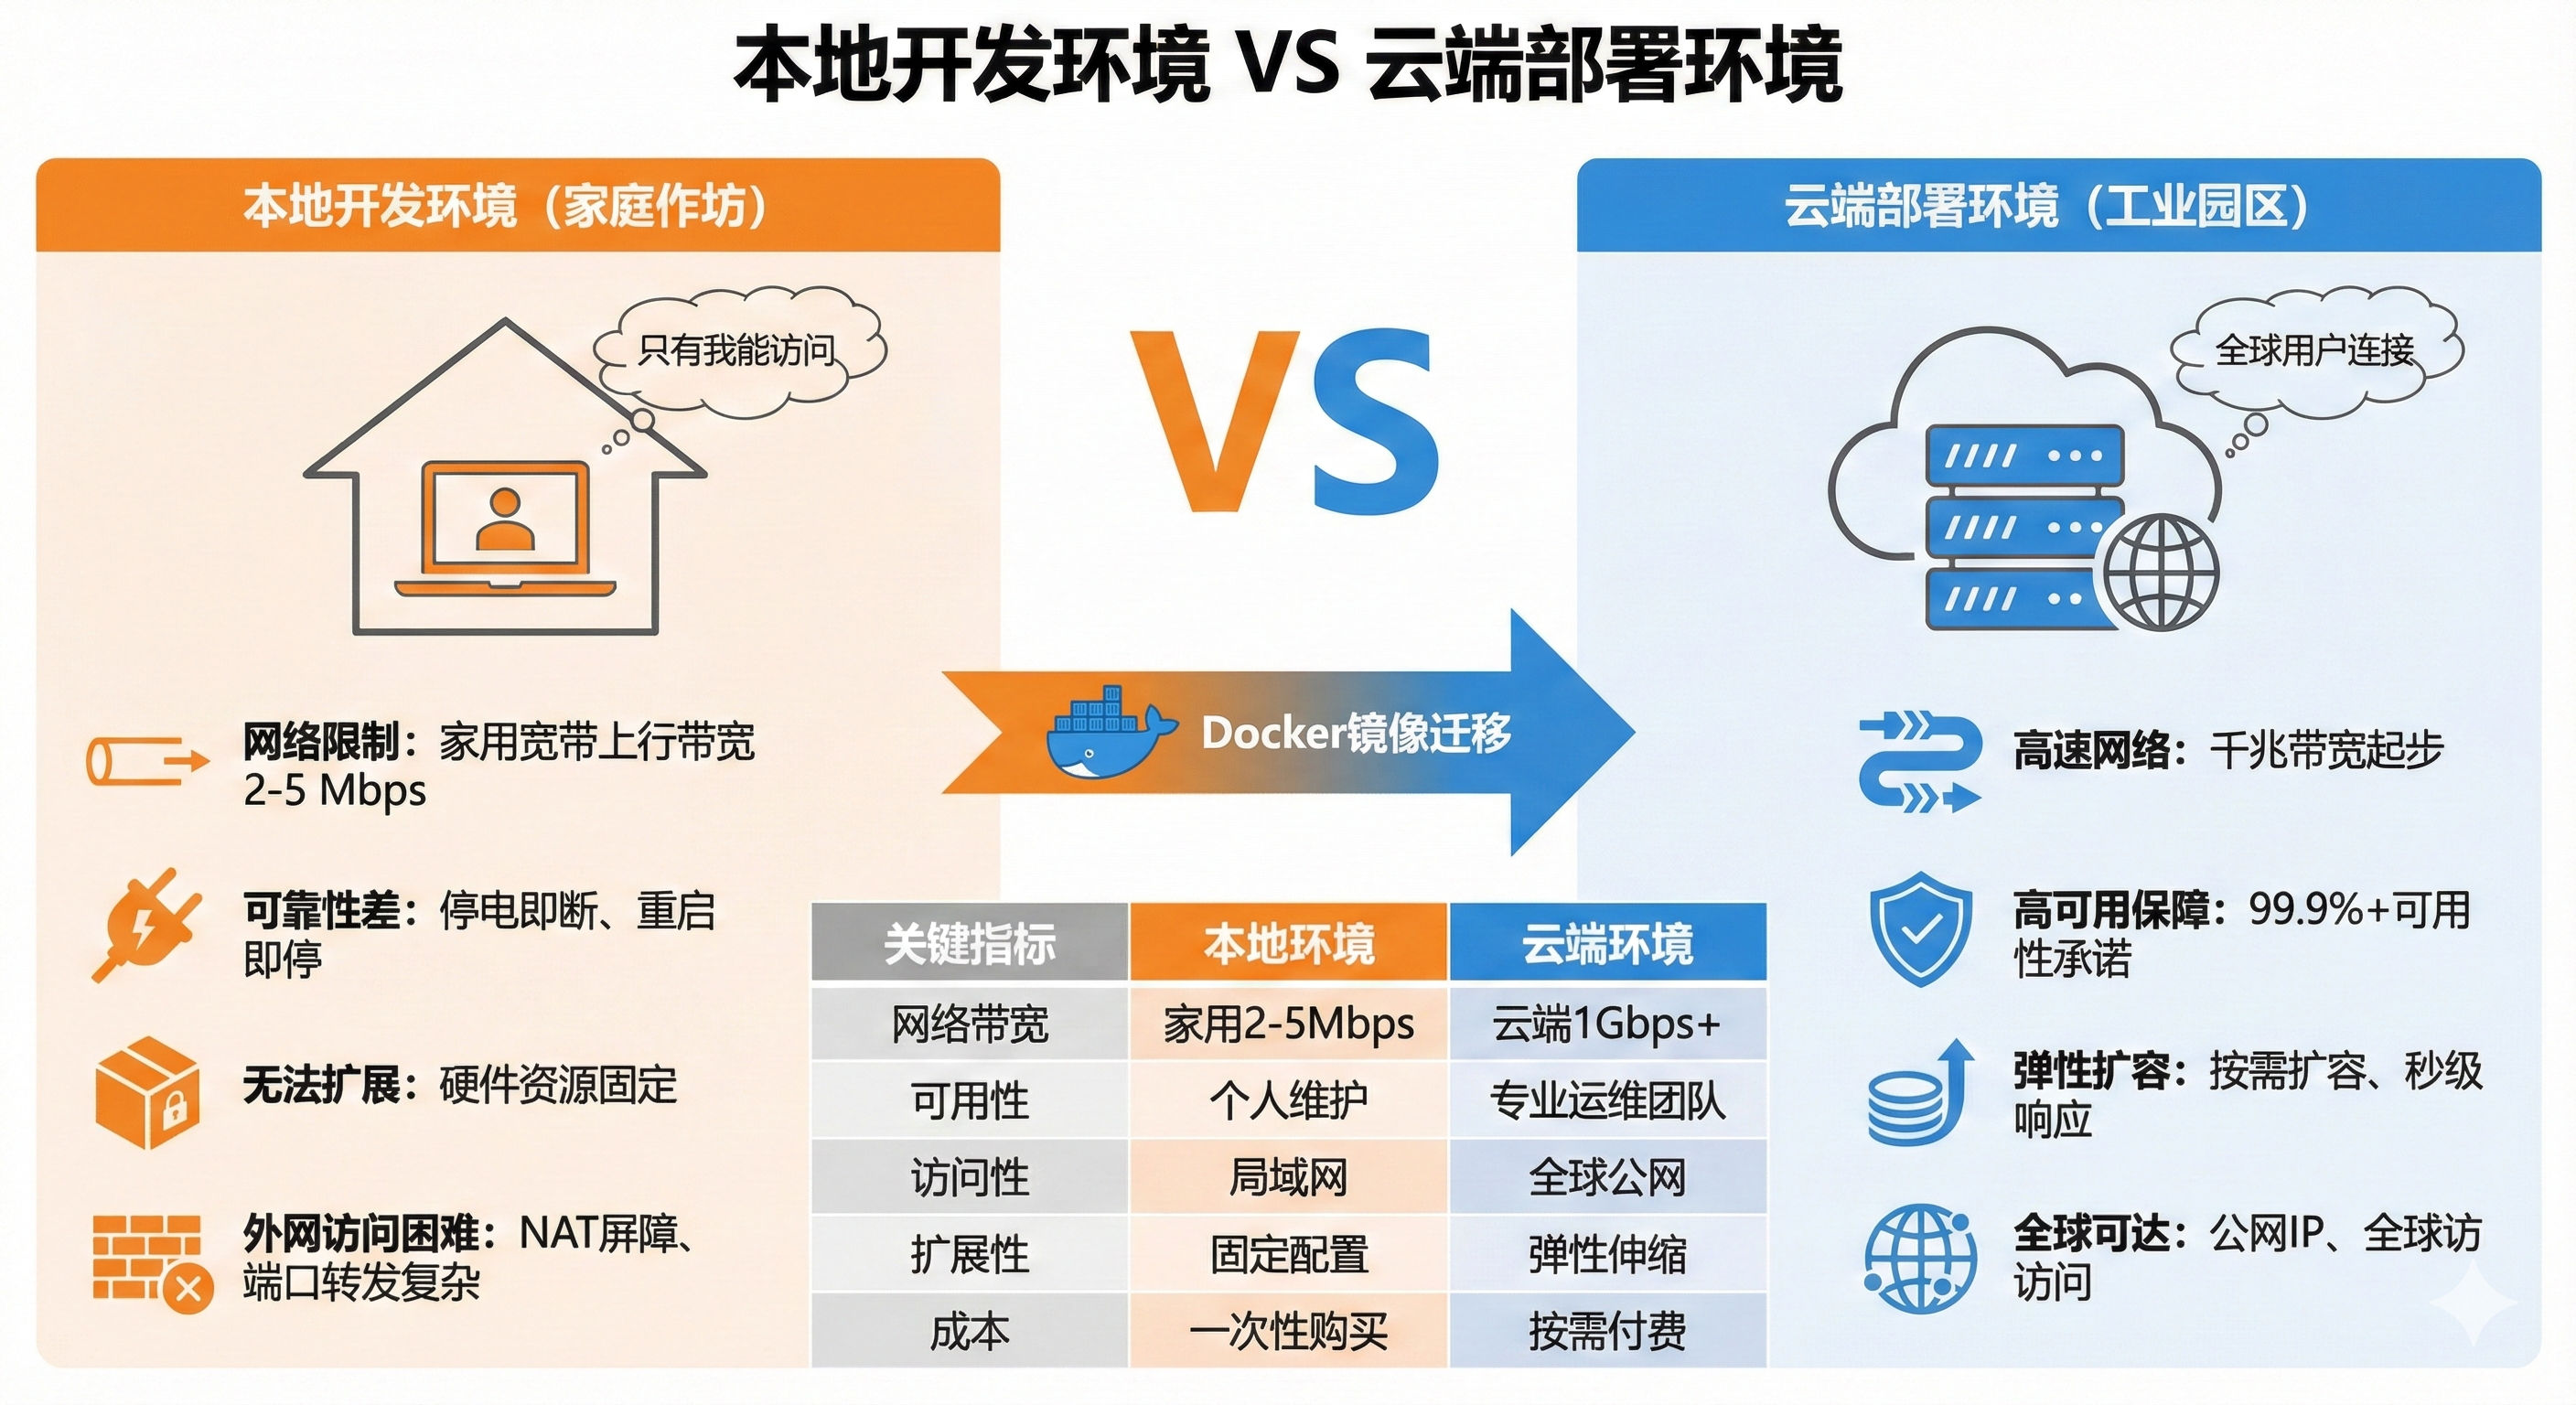
\includegraphics[width=0.9\textwidth]{figures/sec5/local-vs-cloud-environment.png}
\caption{本地开发环境与云端部署环境的全面对比}
\label{fig:local-vs-cloud}
\end{figure}

如图\ref{fig:local-vs-cloud}所示，从家庭作坊式的本地开发环境向工业级的云端部署环境迁移，不仅仅是硬件配置的提升，更是从个人实验向商业服务的根本转变。

\subsubsection{选择云端战场：配置你的虚拟战舰}

在决定将游戏世界搬到云端之后，我们面临的第一个实际问题就是：到底该选择什么样的云服务器？这个决策看似复杂，实际上可以用一个简单的对比来理解——就像从家里的小作坊升级到工业园区的标准厂房。

我们之前在本地开发时使用的个人电脑，就像是自己家里的一间小作坊：电源稳定性一般（停电就断），网络带宽有限（家用宽带上行只有几Mbps），而且只有你自己能进入（局域网访问）。更要命的是，一旦你的电脑关机或重启，整个“作坊”就停止运营了，所有的“客户”都会被拒之门外。

而云服务器则完全不同，它更像是工业园区里的标准化厂房：有不间断电源保障，配备高速光纤网络，24小时专业维护团队，全世界的客户都能轻松找到你的地址。最关键的是，如果业务扩张需要更大空间，你可以随时申请相邻的厂房进行扩容，而不用重新选址搬迁。

对于我们这种刚刚起步的游戏项目，配置选择其实并不复杂。大部分云厂商都提供了针对不同应用场景的推荐配置，我们只需要按照官方的入门指南来选择即可。通常来说，支持几十到几百名在线玩家的游戏服务，选择2-4核CPU、4-8GB内存的基础配置就足够了。操作系统建议选择Ubuntu 20.04 LTS，因为它对Docker的支持最为成熟，相关的教程和社区资源也最丰富。

更重要的是选择合适的地理位置。如果你的玩家主要在国内，选择华东或华北地区的数据中心能够提供最佳的网络延迟；如果面向海外玩家，则需要选择离目标用户更近的海外节点。这就像开实体店一样，位置的选择直接影响客流量和用户体验。

云服务器的真正价值不在于配置有多强大，而在于它提供的可靠性和可达性保障。当我们的游戏世界部署在云端后，它就变成了一个真正的“永不下线”的在线世界，全球的玩家都能随时随地进入并享受稳定的游戏体验。

\subsubsection{理解上云本质：从孤岛到互联网}

上云的核心不是简单的“换个地方放服务器”，而是一次架构思维的根本转变。在本地开发阶段，我们构建的是一个“孤岛式”的封闭系统：所有组件都在同一台机器上，通过本地网络通信，只有开发者能够访问。而上云意味着将这个封闭系统转变为开放的互联网服务，需要考虑的问题维度完全不同。

从技术架构角度看，上云过程实际上是在解决三个层次的连接问题。第一层是物理连接：确保云服务器具备稳定的网络接入能力，这包括带宽保障、延迟优化以及网络冗余等基础设施问题。第二层是逻辑连接：通过合理的端口映射和防火墙配置，让外部客户端能够正确找到并连接到我们的游戏服务。第三层是业务连接：确保服务在面对真实用户流量时能够稳定运行，这涉及并发处理、错误恢复、性能监控等运维层面的考虑。

更深层次地看，上云还意味着运维模式的转变。本地开发时，我们更多关注的是功能实现和逻辑正确性；而在云端环境中，服务的可观测性、可恢复性、可扩展性变得同样重要。这就需要我们在设计和部署服务时，从一开始就考虑日志收集、健康检查、优雅关闭等生产级特性。

\begin{figure}[htbp]
\centering
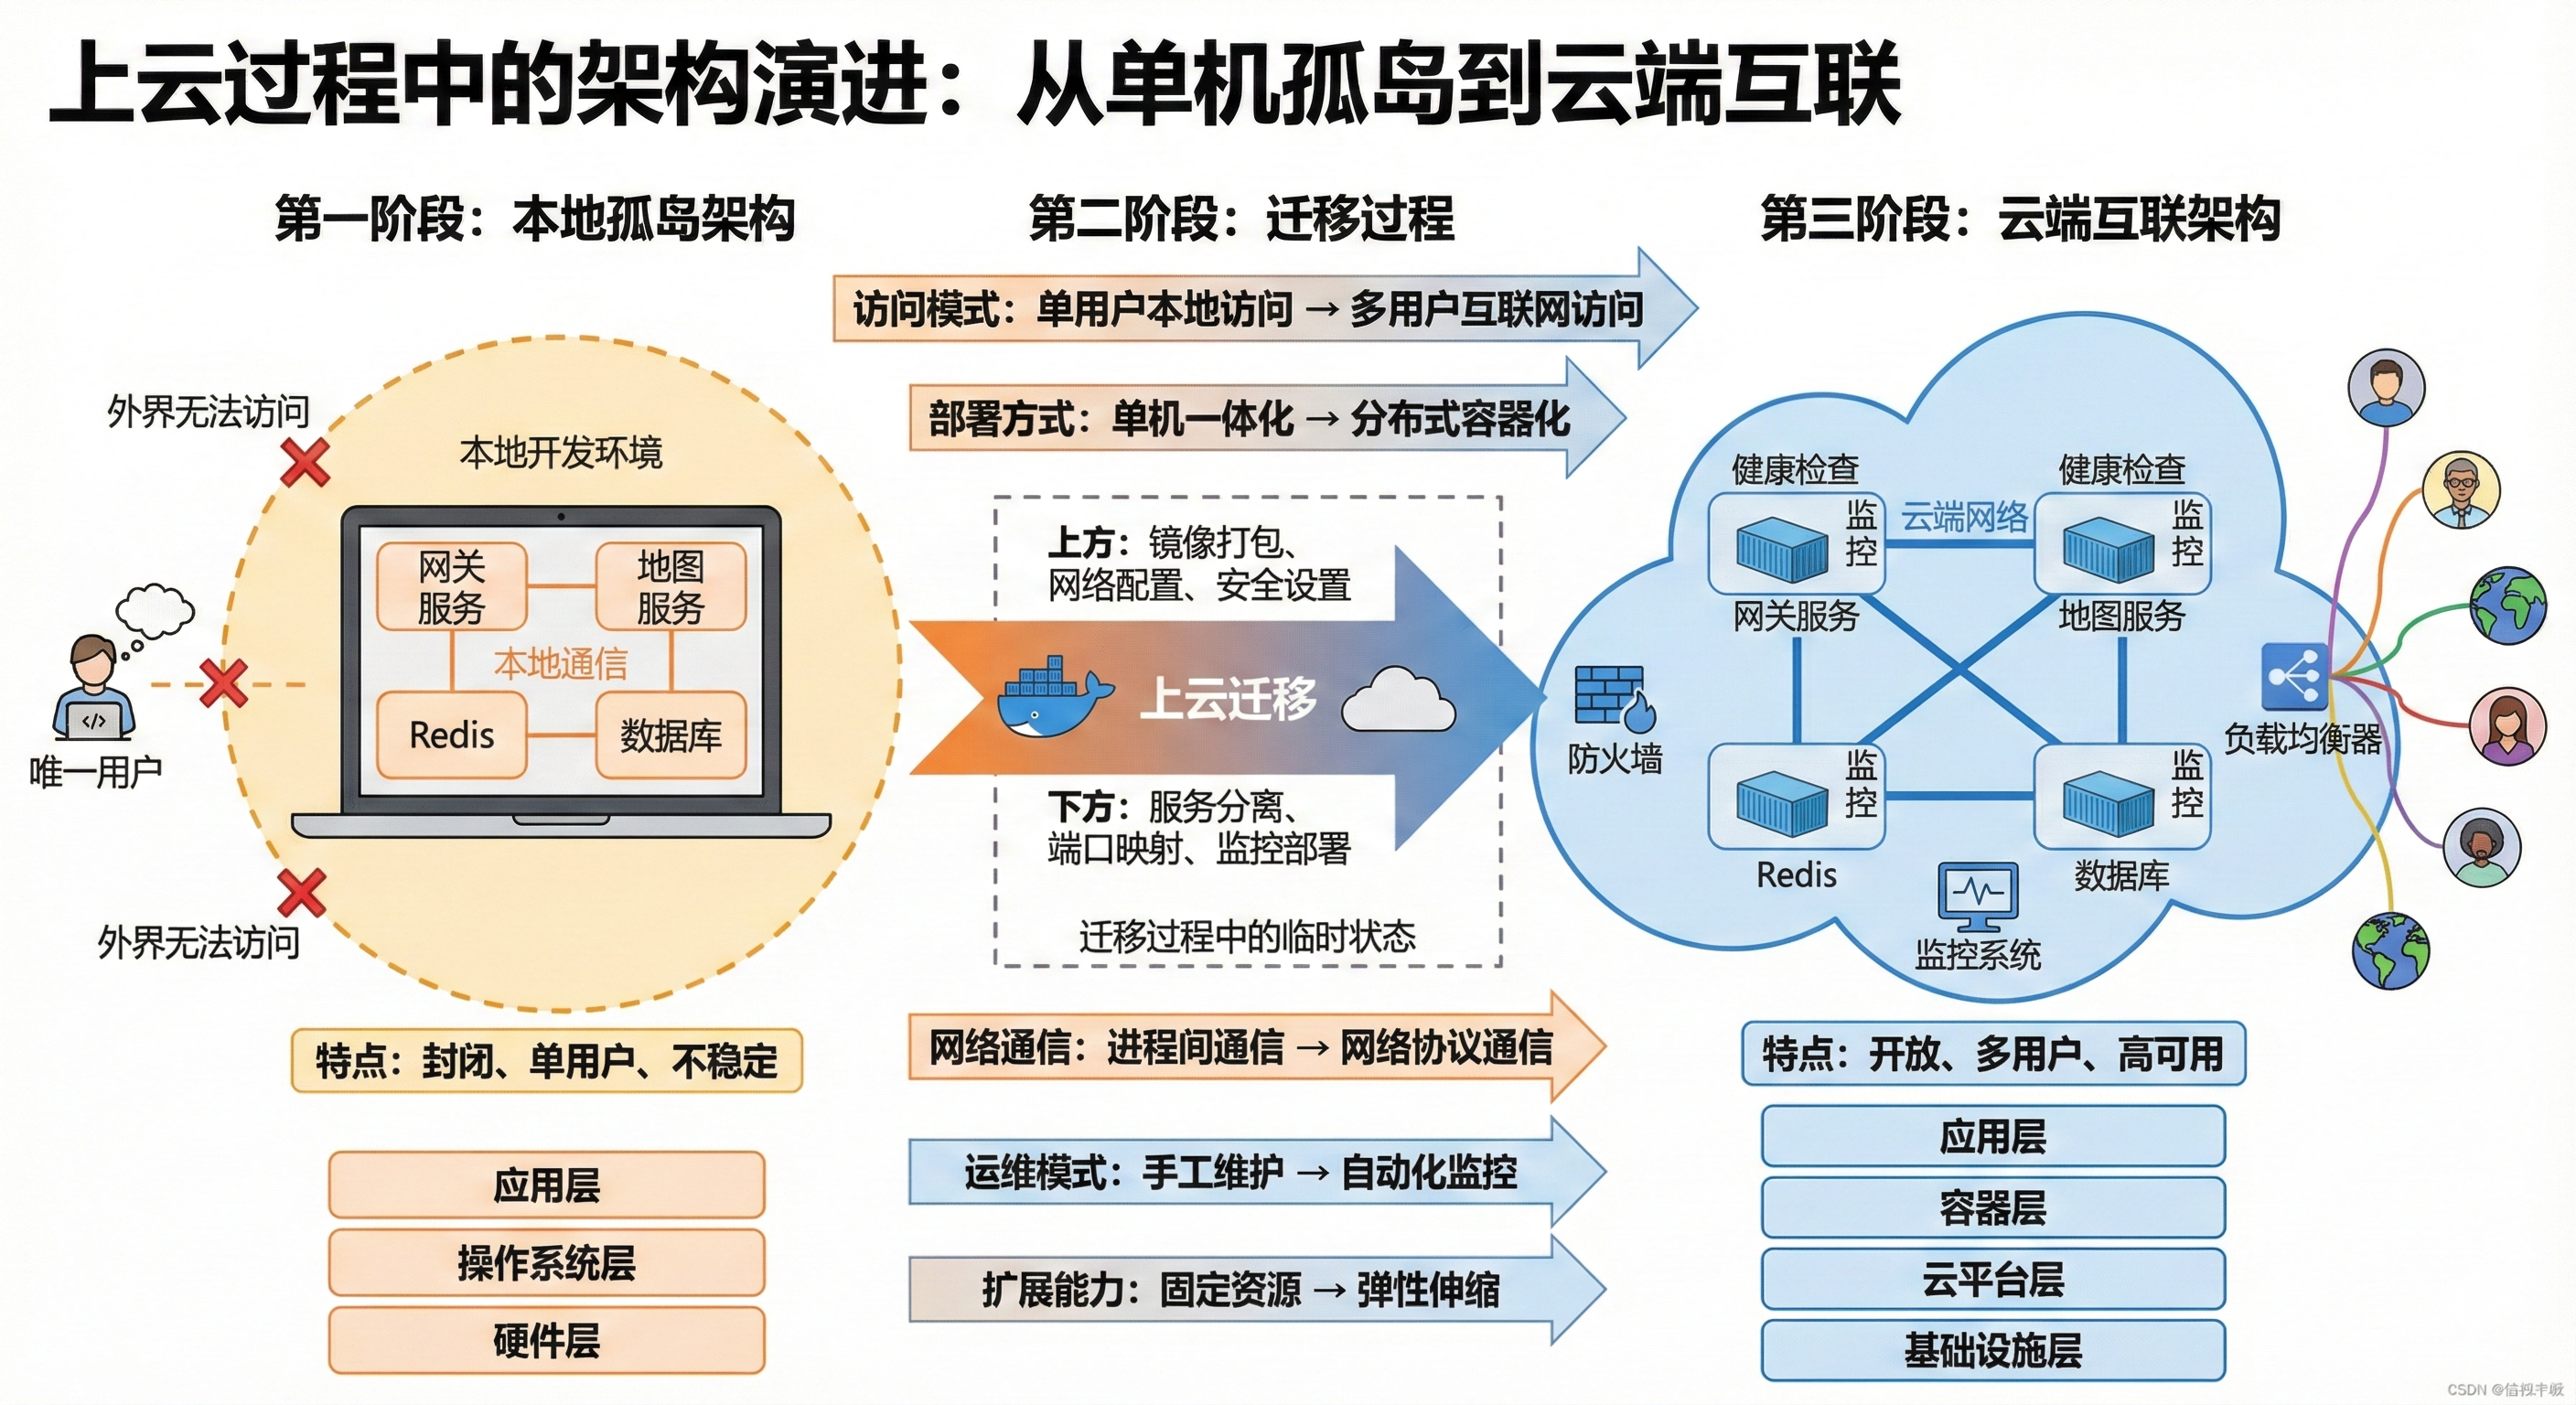
\includegraphics[width=0.9\textwidth]{figures/sec5/cloud-migration-architecture.png}
\caption{上云过程中的架构演进：从单机孤岛到云端互联}
\label{fig:cloud-migration}
\end{figure}

如图\ref{fig:cloud-migration}所示，上云不是简单的平移，而是整个系统架构从封闭走向开放、从静态走向动态的演进过程。

\subsubsection{镜像迁移：代码的跨环境旅行}

将我们在本地构建的Docker镜像传输到云端环境，是上云流程中最关键的技术环节。这个过程的本质是让我们的应用代码完成一次“跨环境旅行”，从开发者的本地机器迁移到云端的生产环境。

这个迁移过程面临着几个核心挑战。首先是传输效率问题：Docker镜像通常体积较大，从几百MB到几个GB不等，如何在有限的网络带宽下快速可靠地完成传输，直接影响部署效率。其次是版本一致性问题：如何确保云端运行的镜像与本地构建的镜像完全一致，避免因为环境差异导致的运行时问题。最后是安全性问题：在镜像传输和存储过程中，如何保护应用代码和敏感配置不被泄露。

最推荐的做法是利用镜像仓库机制来实现镜像的分发。这个过程类似于我们使用应用商店下载手机APP：开发者先将应用上传到商店（推送镜像到仓库），用户再从商店下载到自己设备（从仓库拉取镜像到云服务器）。

镜像仓库的核心优势在于其分层存储机制。Docker镜像本质上是由多个层（Layer）叠加而成的，当我们推送镜像时，仓库会智能地识别哪些层是新的、哪些层是重复的。这意味着后续的版本更新只需要传输变化的部分，大大提升了传输效率。

在选择镜像仓库时，我们有多种选择。Docker Hub是最常用的公共仓库，免费用户可以创建无限数量的公开镜像，但私有镜像数量有限制。各大云厂商也提供了自己的容器镜像服务，如阿里云的容器镜像服务ACR、腾讯云的容器镜像服务TCR等，这些服务通常提供更好的国内访问速度和更丰富的企业级功能。

\begin{figure}[htbp]
\centering
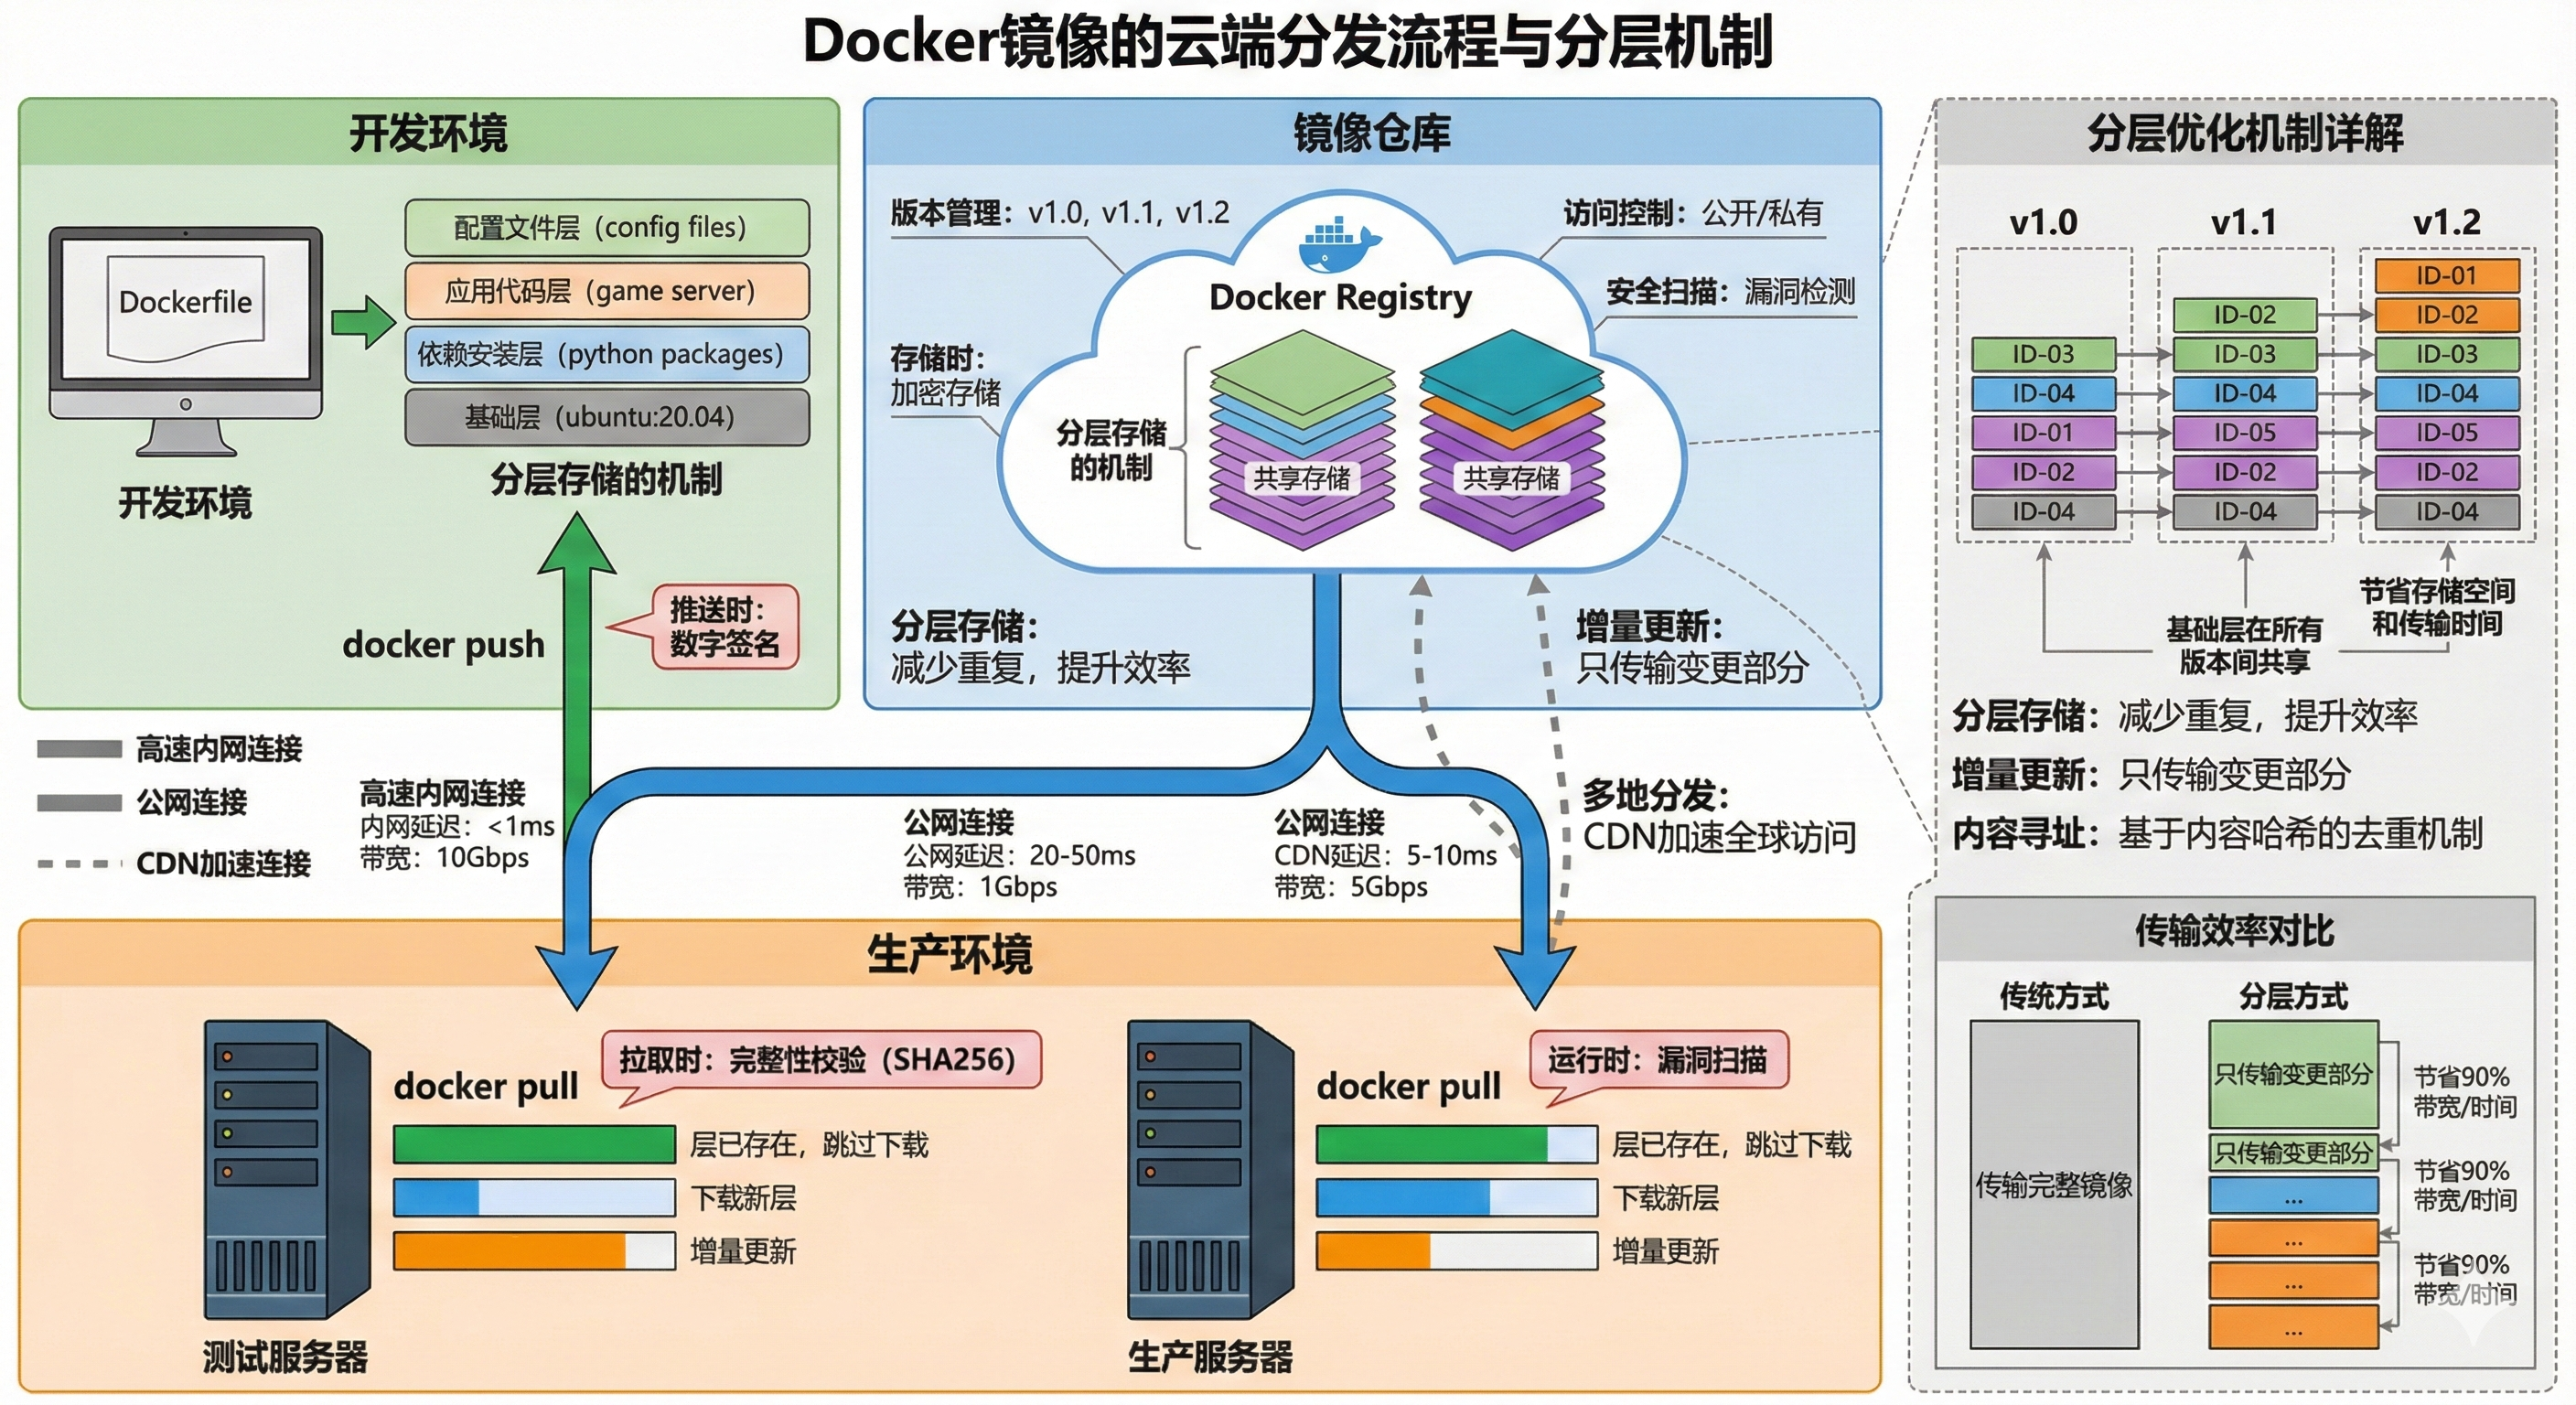
\includegraphics[width=0.9\textwidth]{figures/sec5/docker-image-distribution.png}
\caption{Docker镜像的云端分发流程与分层机制}
\label{fig:image-distribution}
\end{figure}

对于对安全性要求较高或网络环境特殊的场景，也可以选择直接文件传输的方式。这种方法将镜像导出为文件，然后通过文件传输工具将其上传到云服务器，最后重新导入镜像。虽然这种方式缺乏仓库机制的便利性，但在某些企业内网环境或对数据流向有严格管控的场景下，这种点对点传输方式反而更加合适。

无论采用哪种传输方式，都强烈建议在传输完成后进行完整性校验。通过比较本地和远程镜像的摘要值，可以确保传输过程中没有发生数据损坏。这种看似多余的验证步骤，往往能在关键时刻避免因为镜像损坏导致的莫名其妙的运行时错误。

\subsubsection{网络配置：为服务打开通往世界的大门}

成功将镜像传输到云端并启动服务后，最后一个关键步骤就是配置网络访问策略。如果说镜像迁移是让应用“安家落户”，那么网络配置就是为这个新家“开门接客”的过程。

云环境的网络安全机制相比本地环境要严格得多，遵循的是“默认拒绝，显式允许”的安全原则。这意味着新启动的云服务器几乎所有端口都是关闭的，我们需要根据业务需求，显式地为每个需要对外提供服务的端口开放访问权限。

云厂商通常通过“安全组”（Security Group）机制来管理网络访问规则。安全组本质上是一套网络防火墙规则的集合，可以精确控制哪些来源IP、哪些端口、哪些协议被允许访问你的服务器。

安全组的工作原理类似于小区的门禁系统。你需要为每类访客（不同类型的网络请求）制定不同的准入规则：普通访客（游戏玩家）可以通过大门（游戏端口）进入；快递员（监控系统）可以通过特定入口（监控端口）送货；而维修人员（运维管理）则需要特殊权限（SSH端口）才能进入核心区域。

对于我们的游戏服务，通常需要配置以下几类规则：HTTP/HTTPS端口用于网页版游戏或API接口访问，WebSocket端口用于实时通信，以及可能的自定义端口用于游戏专有协议。这些服务端口通常需要向全球开放，以便世界各地的玩家都能访问。同时，SSH管理端口应该严格限制访问来源，只允许运维人员的固定IP地址访问。如果架构中包含多台服务器之间的内部通信，这些端口只需要对内网其他服务器开放。

\begin{figure}[htbp]
\centering
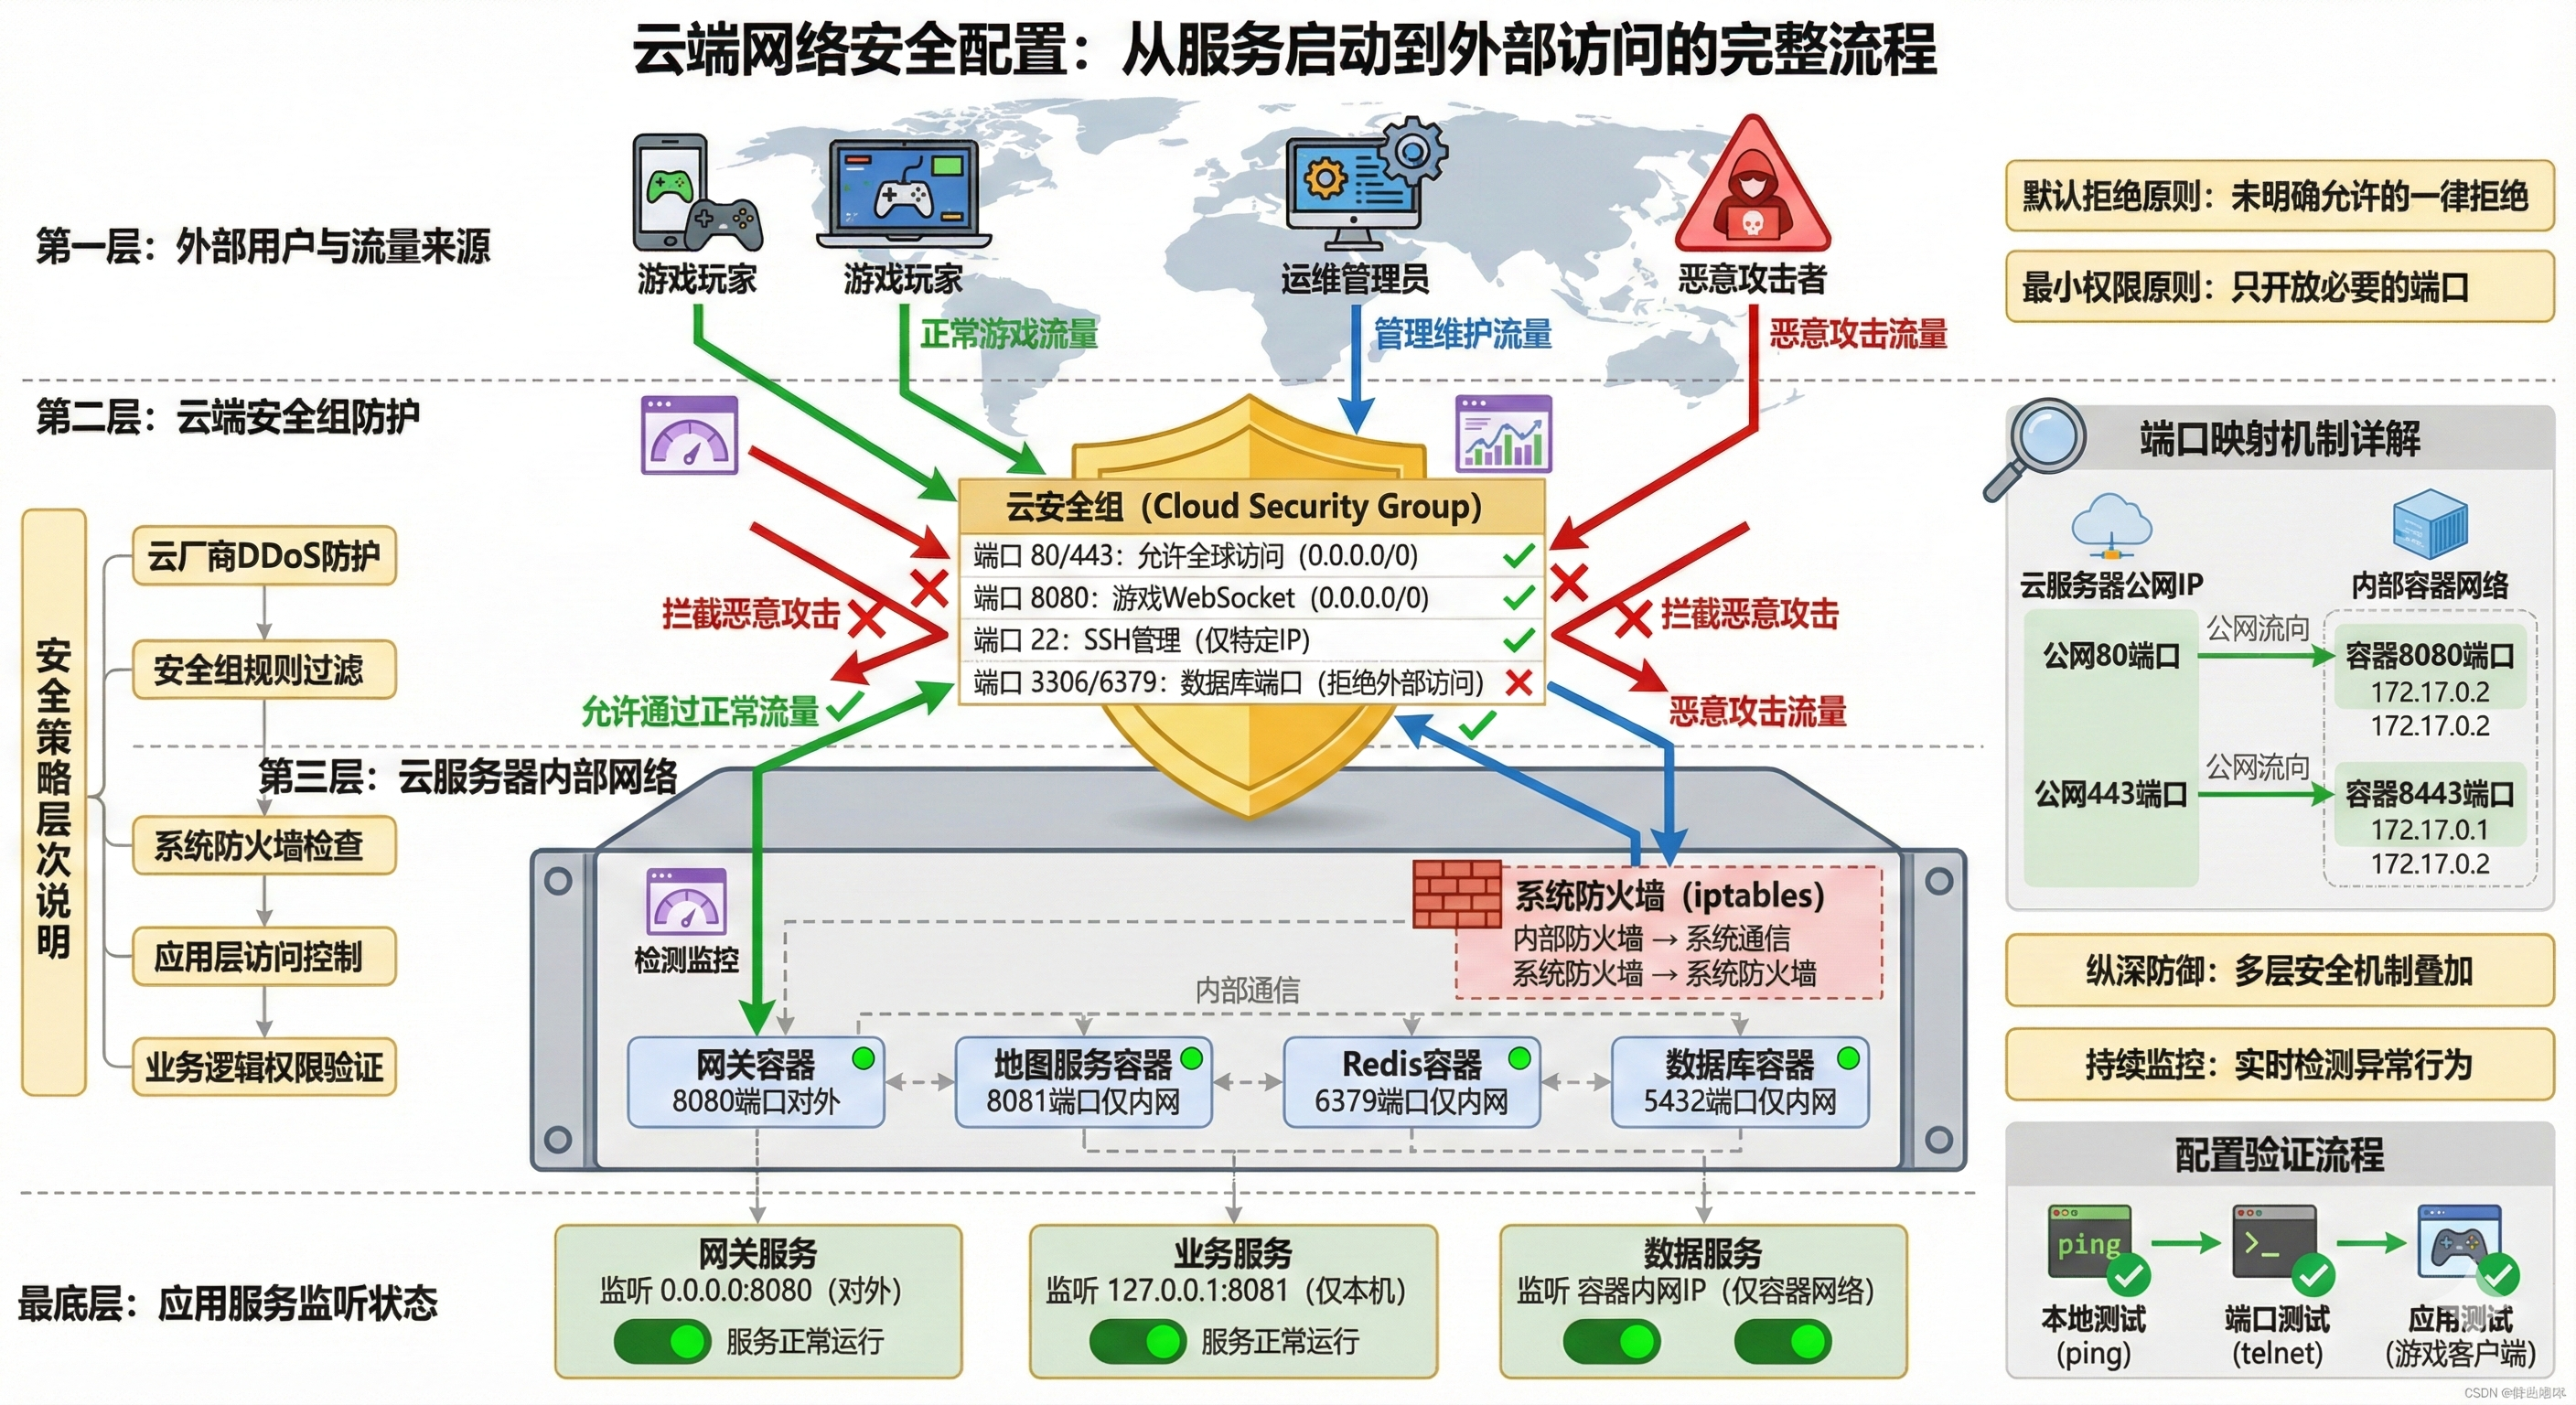
\includegraphics[width=0.9\textwidth]{figures/sec5/cloud-network-security.png}
\caption{云端网络安全配置：从服务启动到外部访问的完整流程}
\label{fig:network-security}
\end{figure}

配置完安全组规则后，强烈建议进行端到端的连通性测试。这个过程就像检查水管是否通畅一样，我们需要确保数据包能够顺利地从外部客户端传输到我们的游戏服务。

测试方法可以从简单到复杂逐步进行。最基础的测试是检查服务器是否可达；进一步可以测试特定端口是否开放；最完整的测试是从实际的游戏客户端发起连接，验证整个应用层协议是否正常工作。

在测试过程中，如果发现连接问题，需要逐层排查：首先检查云服务器的安全组配置是否正确；然后检查服务器内部的防火墙设置；最后确认游戏服务本身是否正常运行并监听在正确的端口上。

通过云端监控工具观察服务器的网络流量、连接数、响应时间等关键指标，也能帮助我们及时发现和解决网络问题。当看到监控面板上出现来自全球各地的连接请求时，就意味着我们的游戏世界真正向全世界开放了。

\subsubsection{从概念到现实：完成上云的最后一跃}

通过以上四个步骤——认识上云价值、选择云端资源、迁移应用镜像、配置网络访问——我们成功地将游戏服务从本地环境迁移到了云端。这不仅仅是一次简单的环境迁移，更是从个人项目向互联网服务的根本转变。

这种转变带来的影响是深远的。从技术角度看，我们获得了更强的可靠性、更好的性能表现、以及面向未来的扩展能力；从产品角度看，游戏从一个只有开发者能体验的原型，变成了全球玩家都能访问的实际服务；从团队角度看，这为后续的协作开发、持续集成、运维监控等工程化实践奠定了基础。

然而，上云只是万里长征的第一步。真正的工业级应用还需要考虑高可用架构、自动化运维、弹性伸缩、灾难恢复等更复杂的技术问题。在接下来的章节中，我们将进一步探索如何利用容器编排、微服务治理等先进技术，让我们的游戏服务具备真正的企业级运维能力。

当你的游戏服务在云端稳定运行，来自世界各地的玩家开始涌入你精心构建的虚拟世界时，那种从创意到现实的成就感，正是每一个技术创造者最珍贵的回报。云端部署不仅仅是技术的升级，更是梦想照进现实的关键一步。

\subsection{Dockerfile逐行详解}
\label{sec:appendix-dockerfile}

本节对第五章5.1节中展示的通用Dockerfile进行逐行解读，帮助读者理解每条指令的具体作用。

这份Dockerfile采用"分层多阶段构建"技术，将整个流程划分为"编译"与"运行"两个阶段。

第1--9行是编译阶段，目标是利用完整的工具链将源代码转化为可执行的二进制文件。第1行与第2行引入包含Go编译器等所有开发工具的官方镜像，命名为builder便于后续引用。3--4行是关键优化：利用Docker基于文件内容的缓存机制，配合Go的依赖管理文件（go.mod）与校验文件（go.sum），只要依赖没有变化，Docker就会直接跳过下载步骤，实现"秒级"热启动。源代码放在依赖构建之后复制，是因为源代码改动最频繁，而Docker的缓存机制是逐层叠加的——如果把源代码放在依赖之前，缓存就会失效。6--7行定义了针对传入参数的服务构建分流逻辑，同时避免构建出空壳镜像。第9行进行静态编译，生成的可执行文件自带所有依赖库，不依赖操作系统的动态链接库，这也是容器可以部署在极简环境中的原因。

后续是生产环境阶段。第10行选择Alpine作为底座，这是一个只有5MB左右的极简镜像。第11行安装时区数据，修正容器默认的UTC时间，确保服务器能正确处理北京时间。14--15行是构建过程的精髓：\texttt{COPY --from=builder}仅从第一阶段提取编译好的可执行文件与配置文件，将源代码和编译器全部丢弃。最后一行定义容器启动时默认执行的命令。

\subsection{Kubernetes部署实战}
\label{sec:appendix-k8s-deploy}

本节将第五章5.4节中的实战操作步骤独立出来，供读者在理解K8s核心概念后动手实践。

理解了Kubernetes的工作原理后，让我们通过实际的部署过程来体验其强大能力。整个部署过程体现了"声明期望，自动实现"的云原生理念。

部署准备的第一步是确保镜像资源就绪。我们需要将游戏服务的Docker镜像推送到Kubernetes集群可以访问的镜像仓库中。这个步骤延续了我们在容器化阶段建立的标准化流程，确保集群中的任何Node都能获取到相同的镜像版本。

第二步是编写声明式配置文件。Kubernetes使用YAML格式的配置文件来描述期望状态，这些配置文件包含了资源定义、依赖关系、约束条件等所有必要信息。对于我们的游戏服务，主要需要定义Deployment和Service两类资源。

\begin{figure}[htbp]
\centering
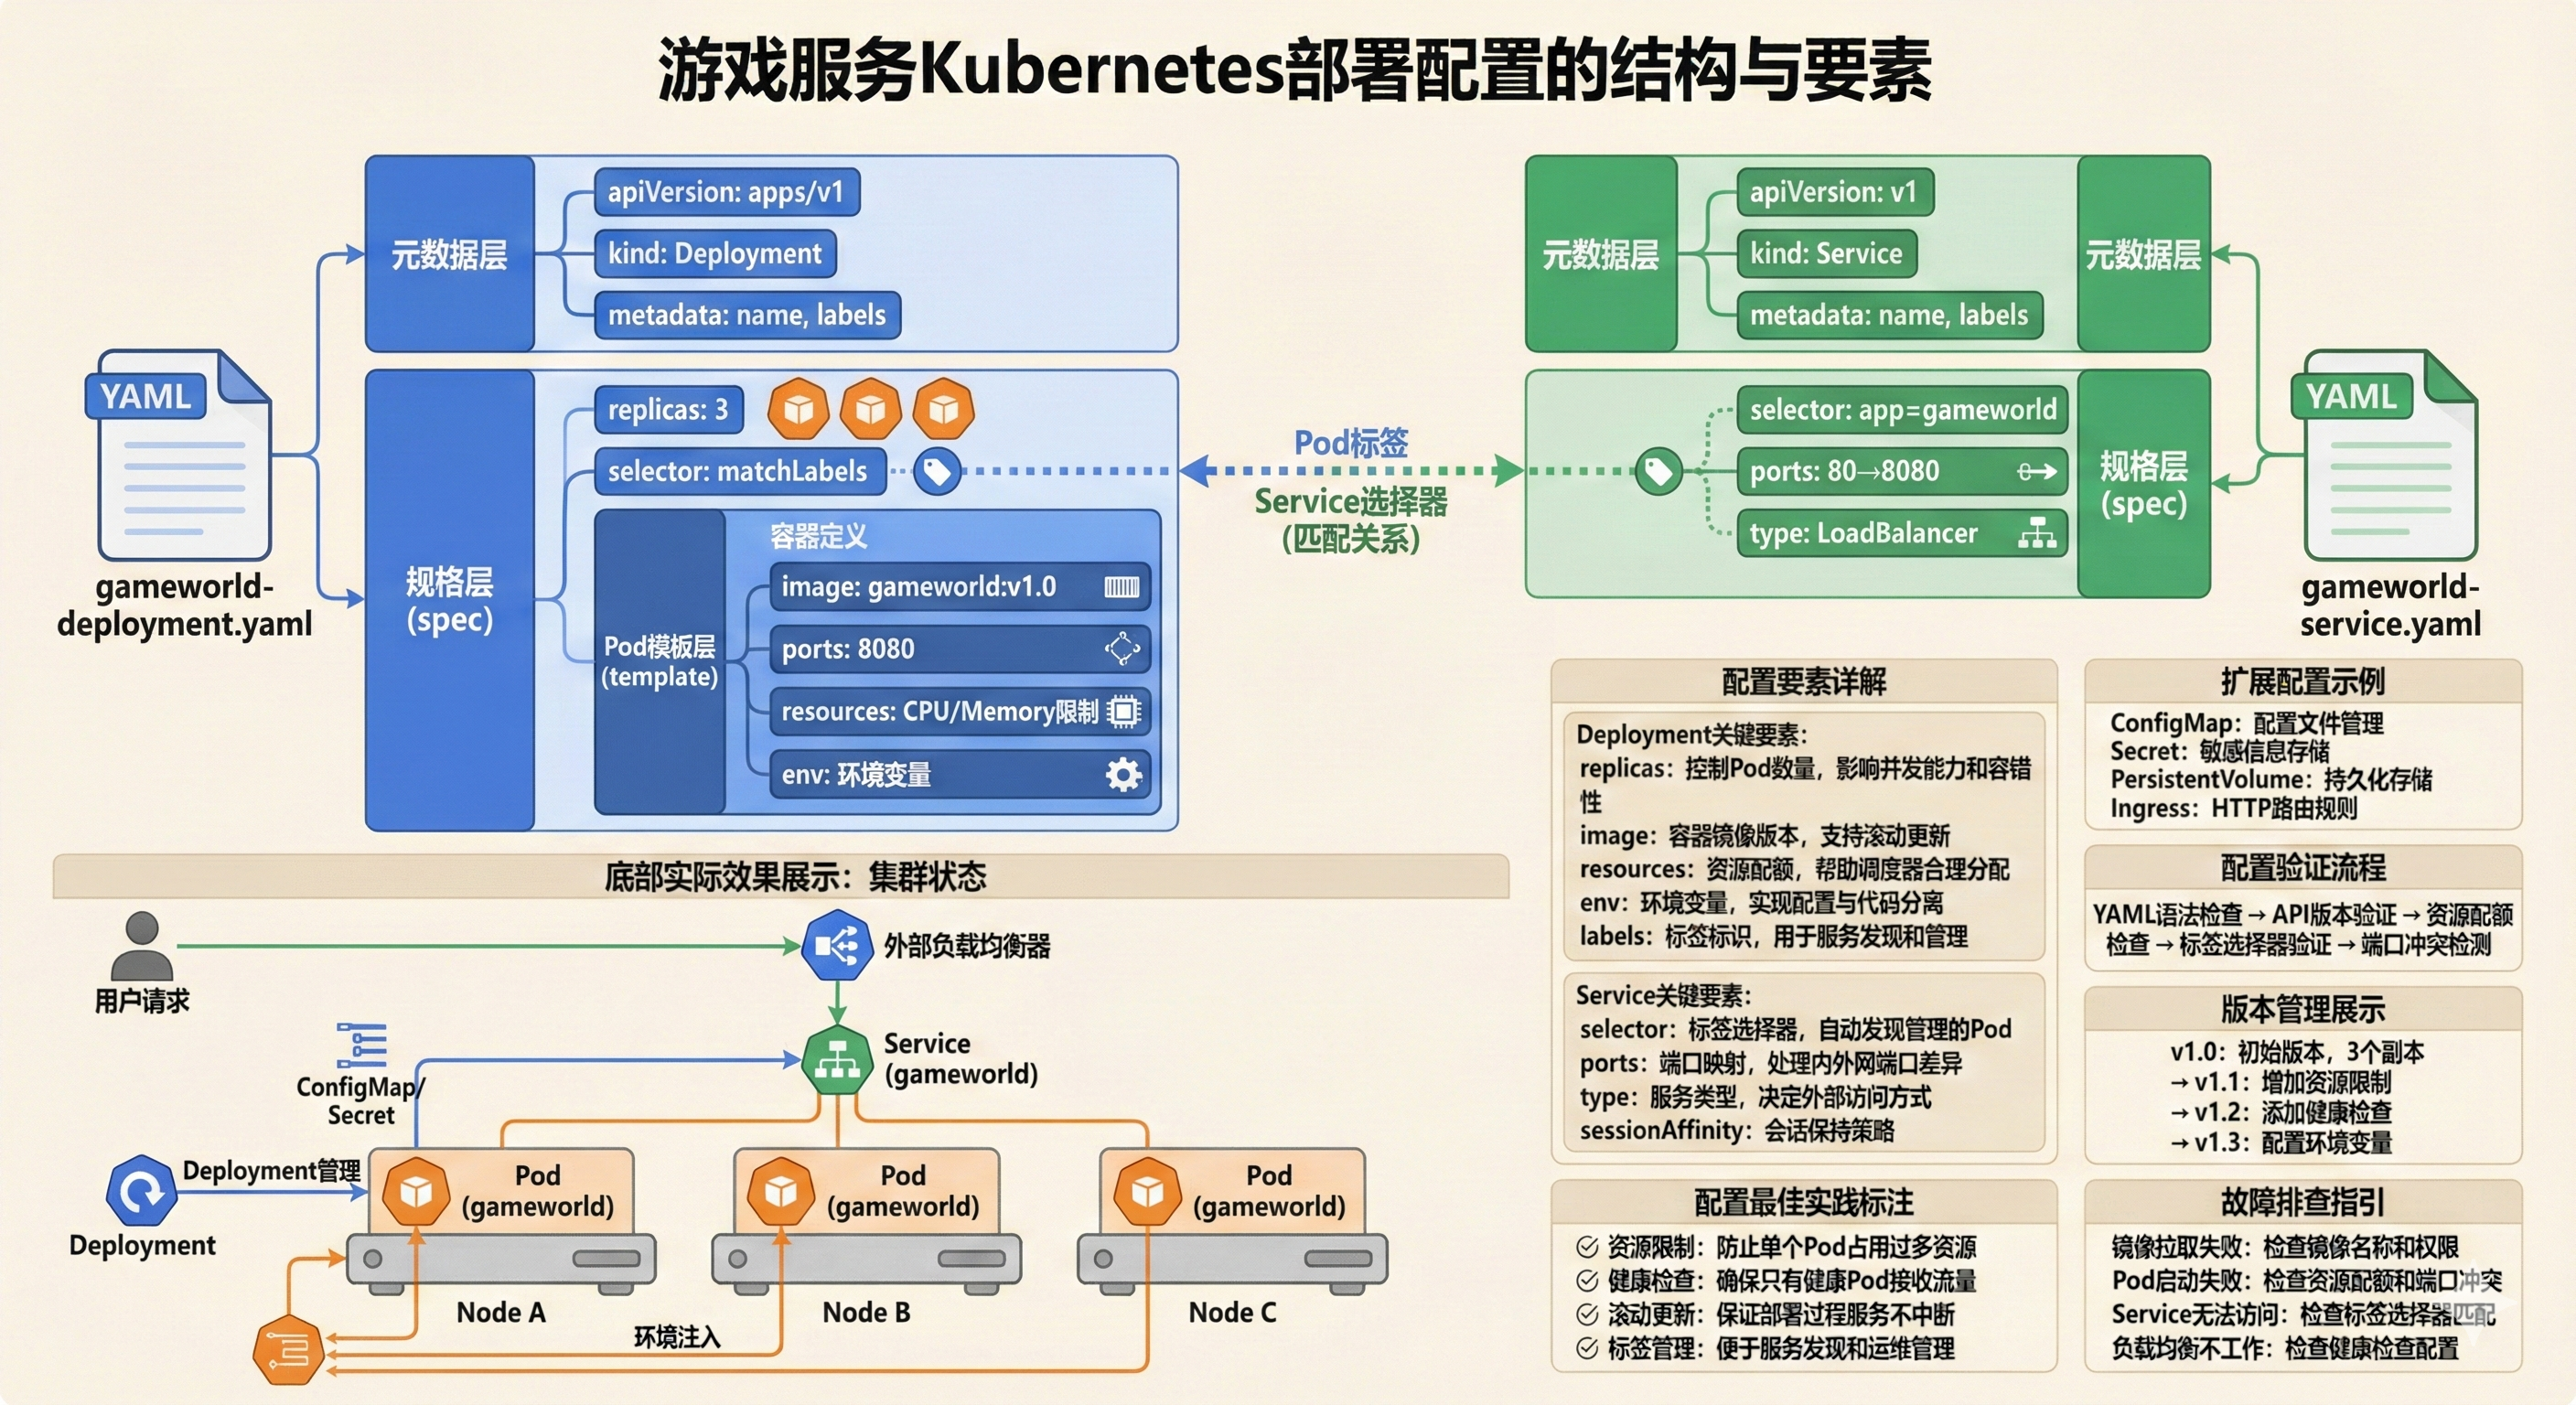
\includegraphics[width=0.9\textwidth]{figures/sec5/kubernetes-deployment-configuration.png}
\caption{游戏服务Kubernetes部署配置的结构与要素}
\label{fig:k8s-config}
\end{figure}

如图\ref{fig:k8s-config}所示，Deployment配置定义了Pod模板、副本数量、更新策略、资源限制等关键参数。副本数量决定了系统的并发处理能力和容错级别；资源限制帮助调度器进行合理的资源分配；更新策略确保版本升级时的服务连续性。这种配置方式将复杂的运维决策转化为了清晰的参数设置，大大降低了出错的可能性。

Service配置定义了服务的网络暴露方式、端口映射、负载均衡策略等。通过标签选择器机制，Service能够自动发现并管理所有相关的Pod，形成统一的访问入口。负载均衡器的自动配置让外部流量能够均匀分配到所有健康的Pod实例上，实现了高可用和高性能。

第三步是执行部署命令。通过kubectl命令行工具，我们可以将配置文件提交给Kubernetes API服务器。一旦配置被接受，整个集群就会开始协调工作来实现期望状态。我们可以通过各种kubectl命令来监控部署进度、查看资源状态、调试问题。

\begin{figure}[htbp]
\centering
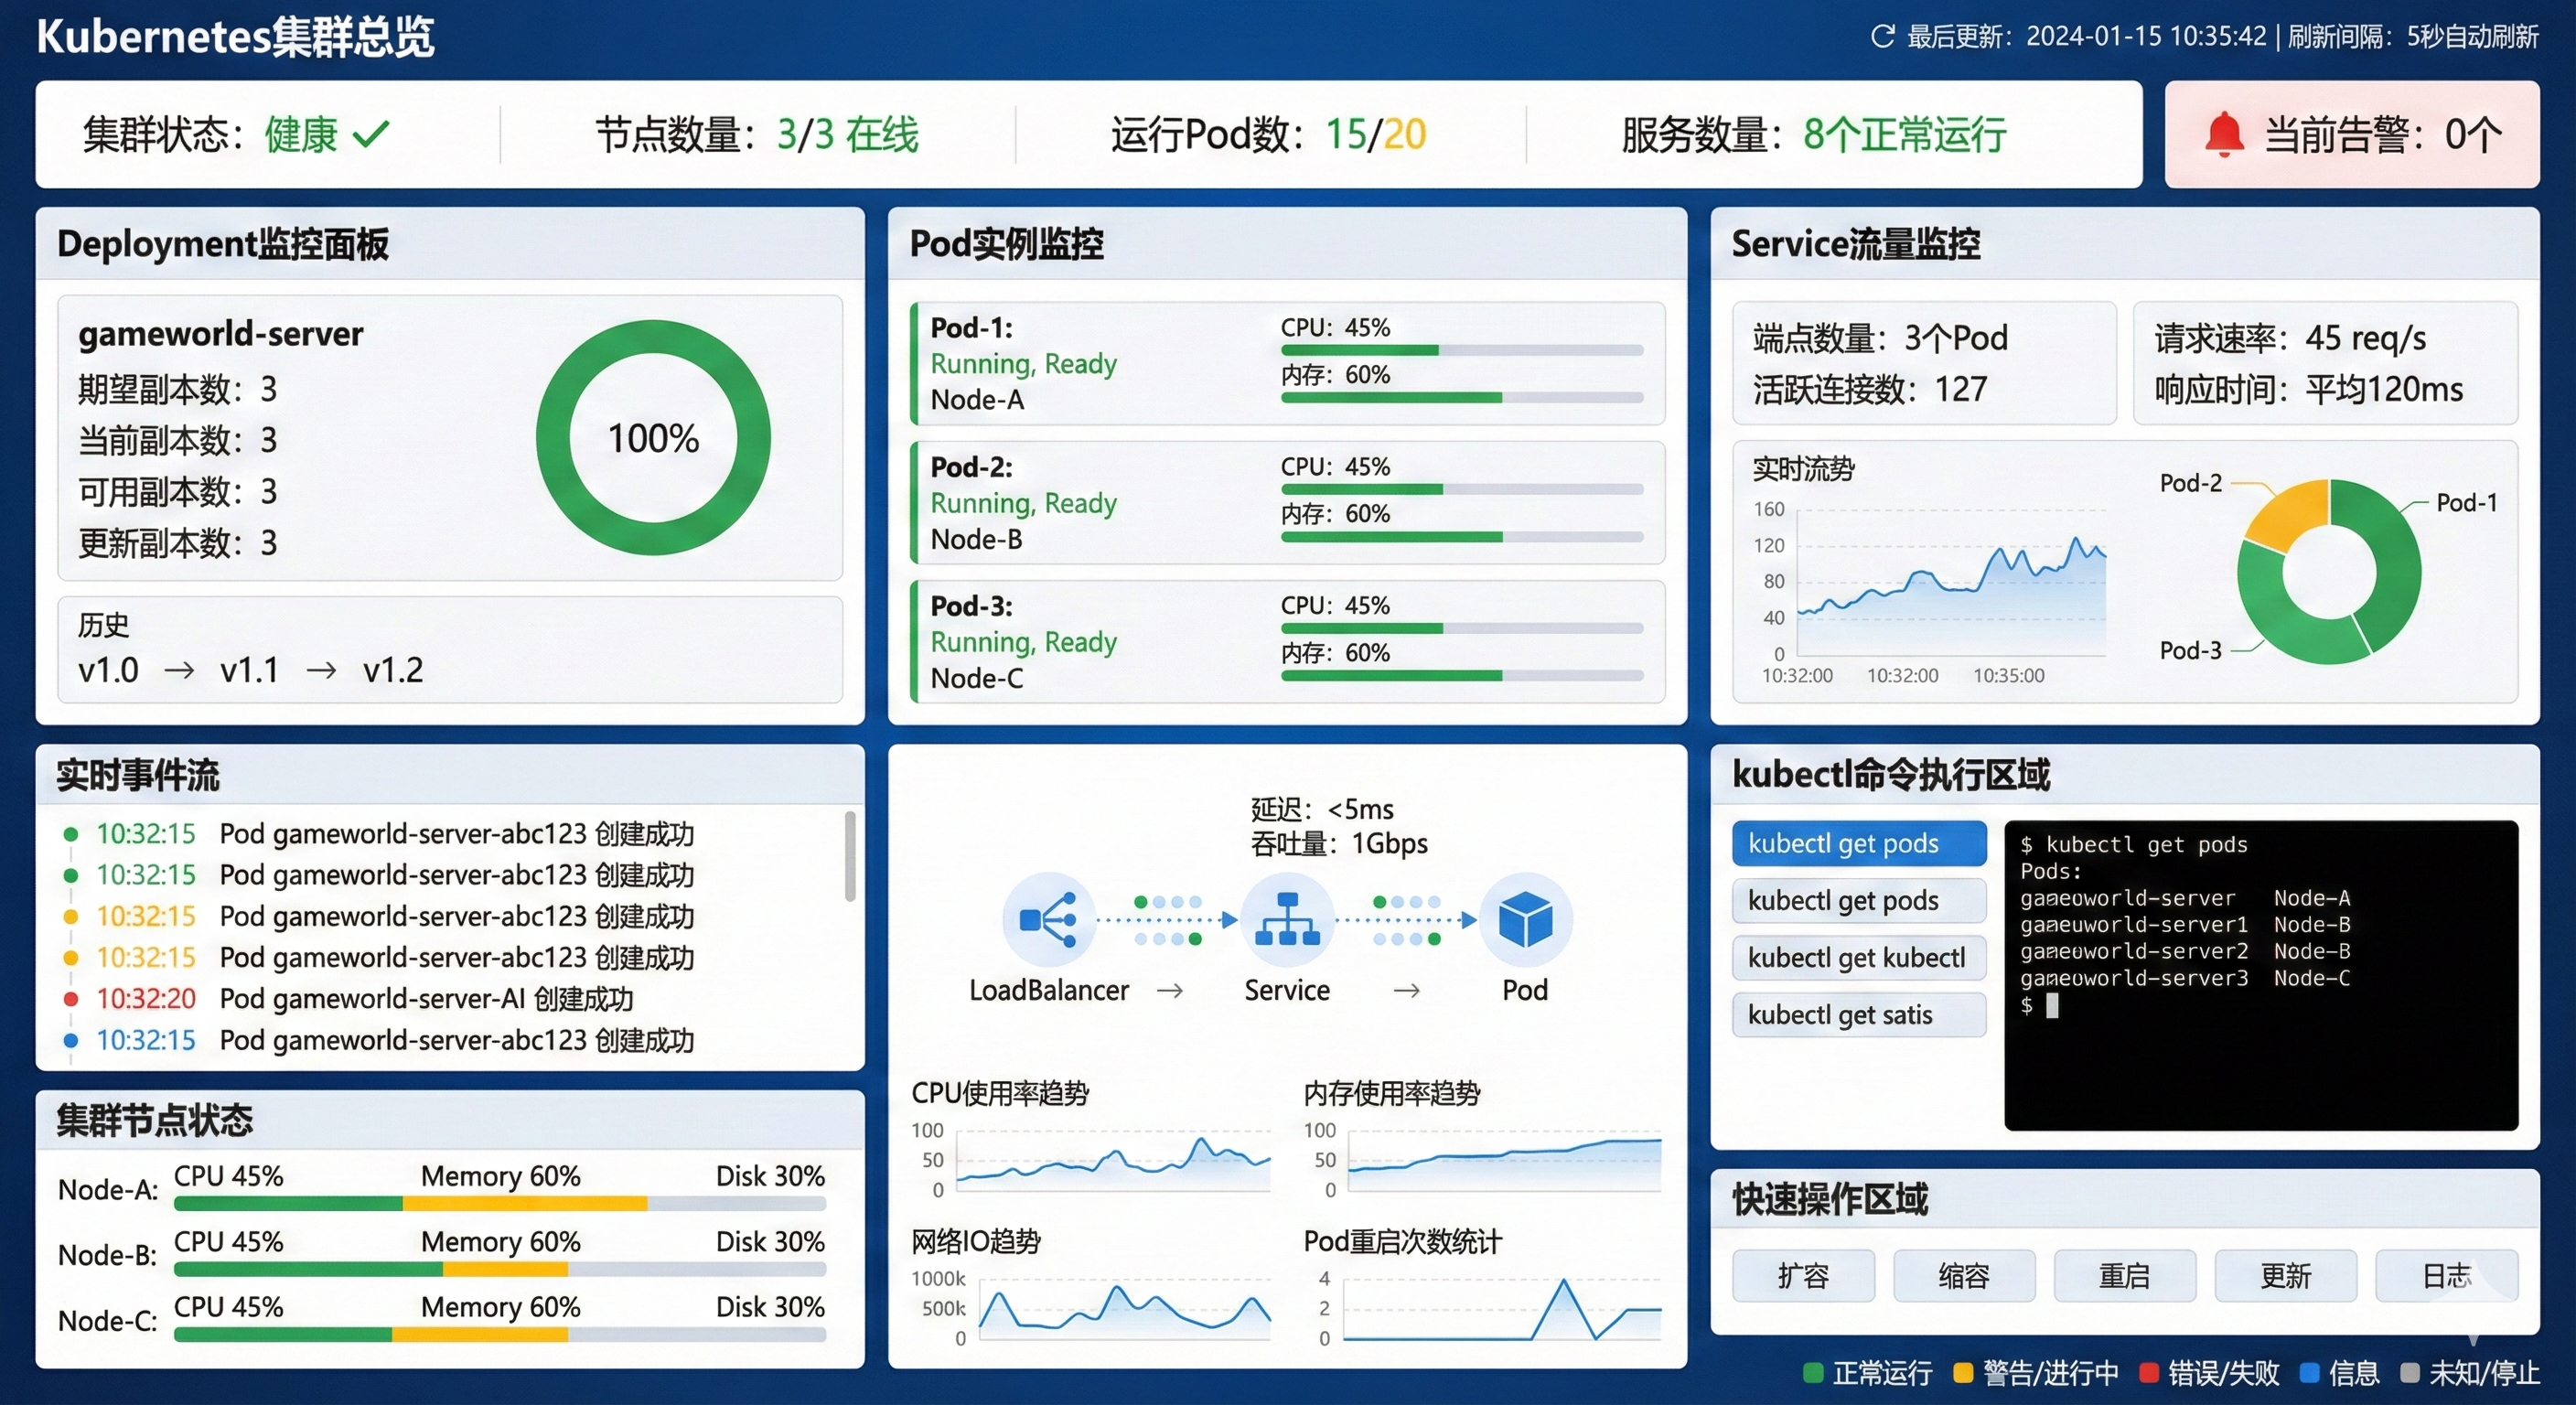
\includegraphics[width=0.9\textwidth]{figures/sec5/kubernetes-deployment-monitoring.png}
\caption{Kubernetes部署过程的监控与状态查看}
\label{fig:k8s-monitoring}
\end{figure}

如图\ref{fig:k8s-monitoring}所示，部署完成后，我们就获得了一个高度自动化的服务运行环境。当需要扩容时，只需修改配置文件中的副本数并重新应用；当需要更新服务版本时，只需修改镜像标签并执行滚动更新；当某个Pod出现故障时，Kubernetes会自动重启或替换。这种自动化程度让运维工作从"被动响应"转变为"主动配置"，大大提升了效率和可靠性。

通过这一节的学习，我们已经掌握了Kubernetes的核心理念和基本使用方法。但这仅仅是容器编排世界的入门，Kubernetes还提供了配置管理、服务网格、监控告警等更高级的功能。

当你看到kubectl命令返回"deployment successfully deployed"的提示时，意味着你已经成功将应用从单机模式升级到了分布式集群模式。此时的游戏服务不再依赖于单台服务器的稳定性，而是由整个Kubernetes集群的智能调度和自动恢复能力来保障，这是向云原生架构迈出的关键一步。

\section{实验操作指南}
\label{sec:appendix-lab-guide}

本附录为第二章至第四章提供配套的实验操作指南。正文侧重于架构原理与设计决策的阐述，本附录则聚焦于具体的代码实现与动手实践，帮助读者将理论知识转化为可运行的工程原型。每个实验均提供核心代码片段与设计说明，读者可在此基础上自行扩展和定制。

\subsection{第二章实验指南：双人对战原型}

本节对应第二章的CS架构双人对战原型，涵盖TCP服务器搭建、协议设计、状态持久化与终端客户端四个实验模块。

\subsubsection{实验一：TCP服务器与连接管理}

第二章正文介绍了连接管理的职责：会话标识、心跳检测与超时清理。本实验展示如何用Go标准库\texttt{net}包实现一个支持多客户端接入的TCP服务器骨架。

核心设计要点：
\begin{itemize}
\item 服务器通过\texttt{net.Listen("tcp", addr)}绑定端口，在主循环中调用\texttt{Accept()}等待新连接
\item 每个新连接启动独立的Goroutine处理（对应第三章的One Goroutine Per Connection模式）
\item 为每个连接分配递增的整数ID，并维护\texttt{map[int]*clientConn}映射表
\item 客户端连接结构体封装网络句柄、JSON编解码器、发送通道与心跳时间戳
\item 独立的心跳监控Goroutine每2秒扫描一次，超过15秒未收到消息的连接判定为超时并清理
\end{itemize}

\begin{tcolorbox}[title=服务器连接管理核心结构]
\begin{lstlisting}[style=codeblock, language=go]
type clientConn struct {
    id            int
    conn          net.Conn
    enc           *json.Encoder
    send          chan proto.Message
    lastHeartbeat time.Time
}

func (s *Server) Start() error {
    ln, err := net.Listen("tcp", s.addr)
    go s.monitorHeartbeats() // 心跳监控协程
    for {
        conn, _ := ln.Accept()
        go s.handleConn(conn) // 每连接一协程
    }
}
\end{lstlisting}
\end{tcolorbox}

\subsubsection{实验二：JSON协议与消息信封设计}

正文讨论了客户端只能上报``意图''、服务器裁决``结果''的原则。本实验展示如何设计一套覆盖完整对战流程的JSON消息协议。

协议采用``信封模式''（Envelope Pattern）：所有消息共享同一个外层结构体，通过\texttt{Type}字段区分消息类型，不同类型的载荷放在对应的可选字段中。这种设计使得编解码逻辑统一，新增消息类型时只需添加字段而无需修改解析框架。

\begin{tcolorbox}[title=消息信封结构定义]
\begin{lstlisting}[style=codeblock, language=go]
type Message struct {
    Type              string             `json:"type"`
    Join              *Join              `json:"join,omitempty"`
    Move              *Move              `json:"move,omitempty"`
    Challenge         *Challenge         `json:"challenge,omitempty"`
    ChallengeResponse *ChallengeResponse `json:"challenge_response,omitempty"`
    Welcome           *Welcome           `json:"welcome,omitempty"`
    State             *State             `json:"state,omitempty"`
    DeltaState        *DeltaState        `json:"delta_state,omitempty"`
    Info              *Info              `json:"info,omitempty"`
}
\end{lstlisting}
\end{tcolorbox}

消息类型分为两类：客户端上行消息（\texttt{join}、\texttt{move}、\texttt{challenge}、\texttt{challenge\_response}、\texttt{heartbeat}）代表玩家意图；服务器下行消息（\texttt{welcome}、\texttt{state}、\texttt{delta\_state}、\texttt{challenge\_request}、\texttt{challenge\_result}、\texttt{info}）代表权威结果。其中\texttt{state}为全量快照，\texttt{delta\_state}为增量更新，两者配合实现正文所述的混合同步策略。

\subsubsection{实验三：SQLite持久化与断线恢复}

正文第2.4.2节阐述了服务器端持久化的设计原则。本实验展示如何用SQLite实现轻量级的玩家状态存档。

\begin{tcolorbox}[title=持久化存储实现]
\begin{lstlisting}[style=codeblock, language=go]
// 建表：仅存储核心状态字段
CREATE TABLE IF NOT EXISTS players (
    name TEXT PRIMARY KEY,
    x INTEGER NOT NULL,
    y INTEGER NOT NULL,
    hp INTEGER NOT NULL
);

// UPSERT：无论新建还是更新，一条语句搞定
INSERT INTO players (name, x, y, hp) VALUES (?, ?, ?, ?)
ON CONFLICT(name) DO UPDATE
SET x = excluded.x, y = excluded.y, hp = excluded.hp;
\end{lstlisting}
\end{tcolorbox}

关键实现细节：
\begin{itemize}
\item 使用纯Go实现的SQLite驱动（\texttt{modernc.org/sqlite}），无需CGO编译依赖
\item 每次合法的状态变更（移动、战斗结算）后同步调用\texttt{SavePlayer}
\item 玩家重连时在注册阶段调用\texttt{LoadPlayer}，若存在存档则恢复坐标与生命值
\item 此方案为同步写入，适合双人原型；第三章将演进为Redis缓存+异步写回
\end{itemize}

\subsubsection{实验四：终端客户端与输入验证}

客户端使用\texttt{tcell}库构建终端UI，实现地图渲染、玩家显示、消息提示等功能。核心架构为双Goroutine模型：一个负责从终端读取按键事件，另一个负责从网络接收服务器消息，两者通过\texttt{select}多路复用驱动主循环。

服务器端的输入验证是权威性的关键保障。示例代码中\texttt{isValidInput}函数对每种消息类型进行合法性检查：移动增量限制在$[-1, 1]$范围内防止瞬移；挑战目标ID必须为正整数；曼哈顿距离超过3的挑战请求被拒绝。这些校验逻辑体现了正文所述的``先校验，后执行''原则。

\subsection{第三章实验指南：多人在线服务器}

本节对应第三章的多人在线游戏服务器，涵盖WebSocket接入、Channel事件循环、对象级锁、冷热数据分层存储、缓存同步策略、对象池复用与性能指标收集七个实验模块。相比第二章的TCP双人原型，本章在协议层升级为WebSocket，在并发模型上从全局锁演进为Channel事件驱动，在存储层从单一SQLite演进为Redis+PostgreSQL冷热分离架构。

\subsubsection{实验五：WebSocket服务器与客户端生命周期}

第二章使用原始TCP连接，需要自行处理粘包与分帧。第三章升级为WebSocket协议，由\texttt{gorilla/websocket}库处理帧边界和控制帧，开发者只需关注业务消息。

每个WebSocket连接对应一个\texttt{Client}实例，启动后立即分裂为读写两个Goroutine。读协程从网络接收消息并封装为\texttt{ClientMessage}投递到Hub的Channel；写协程从\texttt{send}通道取出消息写入网络。两个协程通过Channel解耦，互不阻塞。

\begin{tcolorbox}[title=WebSocket客户端核心结构]
\begin{lstlisting}[style=codeblock, language=go]
type Client struct {
    Hub  *hub.Hub
    Conn *websocket.Conn
    send chan []byte  // 有缓冲Channel，流量削峰
    id   string
}

// 非阻塞发送：缓冲区满时丢弃而非阻塞
func (c *Client) Send(data []byte) {
    select {
    case c.send <- data:
    default: // 缓冲区满，丢弃消息
    }
}
\end{lstlisting}
\end{tcolorbox}

关键设计要点：
\begin{itemize}
\item \texttt{send}通道容量设为256，起到流量削峰作用：当网络写入速度跟不上消息产生速度时，消息在通道中排队而非阻塞发送方
\item 写协程通过WebSocket Ping/Pong机制实现心跳检测，\texttt{pongWait}设为60秒，\texttt{pingPeriod}为其90\%
\item 读协程退出时自动向Hub发送注销事件，触发玩家离线清理流程
\item HTTP升级为WebSocket的入口通过\texttt{websocket.Upgrader}实现，\texttt{CheckOrigin}在开发阶段允许跨域
\item 需要注意，这种丢弃策略仅适用于位置更新等可容忍丢失的高频数据。对于金币交易、物品获取等关键事件，应使用阻塞发送或错误处理机制保证可靠投递
\end{itemize}

\subsubsection{实验六：Hub事件循环与Channel通信}

正文第3.2节讨论了从全局锁到Channel事件驱动的演进。本实验展示Hub如何通过三个Channel接收事件，在单个Goroutine中串行处理所有状态变更。

\begin{tcolorbox}[title=Hub事件循环核心结构]
\begin{lstlisting}[style=codeblock, language=go]
type Hub struct {
    mu      sync.RWMutex
    Clients map[Client]bool
    Players map[string]*models.Player

    // 三条事件通道
    Broadcast  chan ClientMessage // 消息处理
    Register   chan Client        // 玩家注册
    Unregister chan Client        // 玩家离线

    // 存储层
    Redis *store.RedisStore
    DB    *store.DBStore
    Cache *store.CacheLayer
}
\end{lstlisting}
\end{tcolorbox}

Hub的\texttt{Run}方法是整个服务器的心脏。它在一个无限\texttt{select}循环中监听三个Channel：\texttt{Register}处理新玩家加入（分配初始坐标、创建Player对象、广播上线通知）；\texttt{Unregister}处理玩家离线（清理连接、持久化状态、广播下线通知）；\texttt{Broadcast}处理所有游戏操作（移动、攻击、拾取物品等）。由于所有事件在同一个Goroutine中顺序执行，对\texttt{Players}和\texttt{Items}映射表的访问天然无竞争，无需加锁。

需要注意的是，Hub仍然保留了\texttt{sync.RWMutex}。这是因为性能指标收集、HTTP状态查询等外部Goroutine可能需要读取玩家列表，此时通过\texttt{RLock}实现安全的并发读取，而Hub主循环中的写操作则使用\texttt{Lock}。这种``Channel为主、锁为辅''的混合策略在实际工程中非常常见。

\subsubsection{实验七：对象级锁与细粒度并发控制}

正文第3.2节阐述了从全局锁到对象级锁的演进思路。本实验展示如何为每个Player对象配备独立的\texttt{sync.Mutex}，使不同玩家的状态修改可以并行执行。

\begin{tcolorbox}[title=Player对象级锁设计]
\begin{lstlisting}[style=codeblock, language=go]
type Player struct {
    ID     string
    X, Y   float64
    HP     int
    Attack int
    Gold   int
    Kills  int
    Alive  bool
    mu     sync.Mutex // 每个玩家独立的锁
}

// 受伤：检查HP-扣减HP-判断死亡 必须是原子操作
func (p *Player) TakeDamage(damage int) {
    p.mu.Lock()
    defer p.mu.Unlock()
    p.HP -= damage
    if p.HP <= 0 {
        p.HP = 0
        p.Alive = false
    }
}
\end{lstlisting}
\end{tcolorbox}

对象级锁的核心价值在于缩小临界区范围。当玩家A攻击玩家B时，只需锁定B的\texttt{mu}来扣减HP，不影响玩家C拾取物品或玩家D移动。示例代码中\texttt{TakeDamage}、\texttt{AddGold}、\texttt{Heal}、\texttt{AddKill}等方法均遵循相同模式：进入时加锁，通过\texttt{defer}确保退出时解锁，方法体内完成``读取-修改-写回''的完整操作。

\subsubsection{实验八：PostgreSQL冷数据Schema设计}

正文第3.3节介绍了冷热数据分离的原则。本实验展示冷数据层的PostgreSQL表结构设计，使用\texttt{gorm}作为ORM框架实现自动建表与类型映射。

示例代码定义了三张核心表：
\begin{itemize}
\item \texttt{UserAccount}：玩家账户表，存储累计金币、击杀数、死亡数等低频变更的统计数据，以\texttt{PlayerID}为唯一索引
\item \texttt{GameAchievement}：成就记录表，采用只增不改的追加模式，通过\texttt{PlayerID}外键关联玩家
\item \texttt{EquipmentConfig}：装备配置表，存储武器、护甲等静态配置数据，读多写少，适合Cache-Aside策略
\end{itemize}

\begin{tcolorbox}[title=gorm模型与连接池配置]
\begin{lstlisting}[style=codeblock, language=go]
type UserAccount struct {
    ID          uint   `gorm:"primaryKey"`
    PlayerID    string `gorm:"uniqueIndex;size:64"`
    TotalGold   int    `gorm:"default:0"`
    TotalKills  int    `gorm:"default:0"`
    TotalDeaths int    `gorm:"default:0"`
}

// 连接池配置
sqlDB.SetMaxOpenConns(50)          // 最大连接数
sqlDB.SetMaxIdleConns(10)          // 空闲连接数
sqlDB.SetConnMaxLifetime(time.Hour) // 连接最大存活时间
\end{lstlisting}
\end{tcolorbox}

连接池的三个参数直接影响数据库的并发承载能力。\texttt{MaxOpenConns}限制同时打开的连接总数，防止数据库过载；\texttt{MaxIdleConns}保持一定数量的空闲连接处于预热状态，避免每次请求都经历TCP握手和认证；\texttt{ConnMaxLifetime}定期回收长期存活的连接，防止连接状态累积异常。读者可根据实际负载调整这些参数。

\subsubsection{实验九：Redis热数据操作}

与PostgreSQL存储冷数据相对，Redis负责存储高频访问的热数据。本实验展示五类典型的Redis热数据操作。

\begin{tcolorbox}[title=Redis热数据操作示例]
\begin{lstlisting}[style=codeblock, language=go]
// 在线状态：String + TTL自动过期
func (r *RedisStore) SetPlayerOnline(playerID string) error {
    key := fmt.Sprintf("player:%s:online", playerID)
    return r.client.Set(r.ctx, key, "1", 5*time.Minute).Err()
}

// 实时位置：Hash结构存储x/y坐标
func (r *RedisStore) UpdatePlayerPosition(playerID string,
    x, y float64) error {
    key := fmt.Sprintf("player:%s:pos", playerID)
    return r.client.HSet(r.ctx, key, map[string]interface{}{
        "x": x, "y": y,
    }).Err()
}

// 排行榜：Sorted Set，Score为击杀数
func (r *RedisStore) UpdateKillCount(playerID string,
    kills int) error {
    return r.client.ZAdd(r.ctx, "leaderboard:kills",
        redis.Z{Score: float64(kills), Member: playerID}).Err()
}
\end{lstlisting}
\end{tcolorbox}

五类操作分别对应不同的Redis数据结构：在线状态使用String加5分钟TTL，玩家掉线后自动过期无需手动清理；实时位置使用Hash存储坐标分量，支持单独更新x或y；排行榜使用Sorted Set，\texttt{ZRevRangeWithScores}可在$O(\log N + K)$时间内返回前K名；HP缓存使用String加TTL；限流使用\texttt{INCR}+\texttt{EXPIRE}组合实现滑动窗口计数器。Redis连接池配置为100个连接、10个最小空闲连接，与PostgreSQL连接池的设计思路一致。

\subsubsection{实验十：缓存策略层实现}

正文第3.3节介绍了三种缓存同步策略的原理与适用场景。本实验展示如何将这三种策略封装为统一的\texttt{CacheLayer}，使上层业务代码无需关心底层同步细节。

\begin{tcolorbox}[title=三种缓存策略的实现骨架]
\begin{lstlisting}[style=codeblock, language=go]
type CacheLayer struct {
    redis *RedisStore
    db    *DBStore
    // Write-Back: 位置数据异步写回缓冲
    positionBuffer map[string][2]float64
    positionMu     sync.Mutex
    // Cache-Aside: 装备配置本地缓存
    configCache    map[string]*EquipmentConfig
    configCacheMu  sync.RWMutex
}

// Write-Through：金币先写DB再写Redis
func (cl *CacheLayer) WriteThroughGold(playerID string,
    goldChange int) error {
    // 先写权威数据源，失败则直接返回
    if err := cl.db.UpdateAccountStats(playerID,
        goldChange, 0, 0); err != nil {
        return err
    }
    // DB成功后再更新缓存
    return cl.redis.UpdateGoldCount(playerID, goldChange)
}

// Write-Back：位置先写Redis，定期批量刷DB
func (cl *CacheLayer) WriteBackPosition(playerID string,
    x, y float64) {
    cl.redis.UpdatePlayerPosition(playerID, x, y)
    cl.positionMu.Lock()
    cl.positionBuffer[playerID] = [2]float64{x, y}
    cl.positionMu.Unlock()
}

// Cache-Aside：装备配置先查缓存，未命中查DB并回填
func (cl *CacheLayer) CacheAsideGetConfig(itemID string)
    (*EquipmentConfig, error) {
    cl.configCacheMu.RLock()
    if cfg, ok := cl.configCache[itemID]; ok {
        cl.configCacheMu.RUnlock()
        return cfg, nil
    }
    cl.configCacheMu.RUnlock()
    cfg, err := cl.db.GetEquipmentConfig(itemID)
    // 回填缓存...
    return cfg, err
}
\end{lstlisting}
\end{tcolorbox}

Write-Back策略的核心是后台刷盘协程。\texttt{CacheLayer}初始化时启动一个独立Goroutine，每5秒将\texttt{positionBuffer}中的脏数据批量写入PostgreSQL。刷盘时先加锁复制缓冲区内容再释放锁，将锁持有时间降到最低。需要注意，Cache-Aside示例中的缓存是进程内的Go map（本地L1缓存），而非Redis。对于装备配置这类读多写少的静态数据，本地缓存可以省去Redis网络往返，进一步降低读取延迟。读路径使用\texttt{RLock}允许并发读取，只在缓存未命中需要回填时才升级为\texttt{Lock}。配置更新时调用\texttt{InvalidateConfigCache}删除缓存条目，下次读取自动从数据库加载最新版本。

\subsubsection{实验十一：sync.Pool对象池复用}

正文第3.3节讨论了高并发场景下频繁内存分配对GC的压力。本实验展示如何用\texttt{sync.Pool}复用JSON序列化所需的\texttt{bytes.Buffer}。

\begin{tcolorbox}[title=sync.Pool复用序列化缓冲区]
\begin{lstlisting}[style=codeblock, language=go]
var bufferPool = sync.Pool{
    New: func() interface{} {
        return bytes.NewBuffer(make([]byte, 0, 256))
    },
}

func MarshalJSON(v interface{}) ([]byte, error) {
    buf := bufferPool.Get().(*bytes.Buffer)
    buf.Reset() // 必须重置，防止脏数据

    err := json.NewEncoder(buf).Encode(v)
    if err != nil {
        bufferPool.Put(buf)
        return nil, err
    }

    result := make([]byte, len(buf.Bytes()))
    copy(result, buf.Bytes())
    bufferPool.Put(buf) // 归还到池中
    return result, nil
}
\end{lstlisting}
\end{tcolorbox}

使用\texttt{sync.Pool}时有两个容易忽略的细节。第一，从池中取出的对象必须调用\texttt{Reset()}清空旧数据，否则会出现数据污染。第二，序列化结果必须复制到新的\texttt{[]byte}后再归还Buffer，因为归还后Buffer的底层数组可能被其他Goroutine覆写。示例代码中\texttt{New}函数预分配256字节容量，减少后续\texttt{grow}操作。在每秒数千次广播的场景下，对象池可将内存分配次数降低一个数量级，显著减少GC暂停时间。

\subsubsection{实验十二：性能指标收集与可观测性}

正文强调了性能验证的重要性。本实验展示如何构建一个轻量级的指标收集器，实时追踪QPS、延迟分布、连接数与GC统计。

示例代码中的\texttt{Metrics}结构体使用\texttt{atomic.Int64}实现无锁的请求计数和连接数追踪，避免在热路径上引入互斥锁开销。延迟分布采用滑动窗口方式保留最近10000个样本，通过排序计算P95和P99百分位数。GC统计直接读取\texttt{runtime.MemStats}，获取当前内存占用、GC次数和最近一次GC暂停时间。

所有指标通过\texttt{/stats}端点以JSON格式暴露，开发者可在浏览器中实时查看服务器运行状态。需要注意，\texttt{runtime.ReadMemStats}会触发短暂的全局暂停以收集一致的内存快照，在生产环境中不宜高频调用；Go 1.16之后可改用\texttt{runtime/metrics}包获取更轻量的指标。这种内建的可观测性机制为后续章节的性能调优和容量规划提供了数据基础。

\subsection{第四章实验指南：分布式模拟器}

本节对应第四章的分布式游戏服务器架构，涵盖数据库分片路由、负载均衡策略与跨服擂台协调三个实验模块。与前两章不同，第四章的示例代码采用单进程模拟器的方式实现：用Goroutine模拟多个服务器节点，用内存数据结构模拟数据库分片和网络通信，无需部署真实的多台机器或外部依赖（不需要Redis、PostgreSQL），运行\texttt{go run main.go}即可观察分布式概念的完整运作过程。

\subsubsection{实验十三：数据库分片路由}

正文第4.1节介绍了三种分片策略的原理与权衡。本实验将这三种策略实现为可插拔的路由器，通过统一的\texttt{Router}接口与业务层解耦。

\begin{tcolorbox}[title=分片路由接口与哈希分片]
\begin{lstlisting}[style=codeblock, language=go]
// 统一路由接口，业务层与分片策略解耦
type Router interface {
    GetShard(playerID int) int
    AddNode(nodeID int)
    RemoveNode(nodeID int)
    GetNodeCount() int
}

// 哈希分片：playerID % N
type HashRouter struct{ nodes []int }

func (r *HashRouter) GetShard(playerID int) int {
    idx := playerID % len(r.nodes)
    return r.nodes[idx]
}
\end{lstlisting}
\end{tcolorbox}

哈希分片的优势在于数据分布均匀，即使玩家ID连续注册也会被打散到不同分片。但扩容时取模基数变化会导致几乎所有数据需要迁移。范围分片按ID区间划分，扩容只需调整边界，但容易产生热点——新注册的活跃玩家集中在最后一个区间。示例代码同时实现了这两种策略，读者可以通过替换\texttt{NewHashRouter}为\texttt{NewRangeRouter}来对比两者的分片分布差异。

\subsubsection{实验十四：一致性哈希与虚拟节点}

正文第4.1节讨论了一致性哈希如何降低扩容时的数据迁移量。本实验展示完整的一致性哈希实现，包括SHA256哈希、虚拟节点映射和环上顺时针查找。

\begin{tcolorbox}[title=一致性哈希核心逻辑]
\begin{lstlisting}[style=codeblock, language=go]
type ConsistentHashRouter struct {
    vnodes int              // 每个物理节点150个虚拟节点
    nodes  map[int]struct{} // 物理节点集合
    ring   map[uint64]int   // 哈希值 -> 物理节点ID
    keys   []uint64         // 排序后的哈希环
}

func (r *ConsistentHashRouter) AddNode(nodeID int) {
    for i := 0; i < r.vnodes; i++ {
        h := sha256Hash(fmt.Sprintf("%d#%d", nodeID, i))
        r.ring[h] = nodeID
    }
    r.rebuildKeys() // 重建排序后的哈希环
}

func (r *ConsistentHashRouter) GetShard(playerID int) int {
    h := sha256Hash(fmt.Sprintf("player:%d", playerID))
    // 在环上顺时针找到第一个 >= h 的节点
    i := sort.Search(len(r.keys),
        func(i int) bool { return r.keys[i] >= h })
    if i == len(r.keys) { i = 0 } // 环形回绕
    return r.ring[r.keys[i]]
}
\end{lstlisting}
\end{tcolorbox}

每个物理节点在哈希环上映射150个虚拟节点，确保即使物理节点数量较少也能实现均匀的数据分布。新增节点时只有环上相邻区间的数据需要迁移，其余数据不受影响。示例代码使用\texttt{crypto/sha256}的前8字节作为哈希值，在教学场景下提供了足够的分布均匀性。生产环境中通常使用MurmurHash或FNV等非加密哈希函数以获得更好的计算性能，此处选择SHA256是为了避免引入第三方依赖。

\subsubsection{实验十五：分片集群与全局排行榜}

正文第4.1.3节讨论了跨分片查询的scatter-gather策略。本实验用内存map模拟多个数据库分片，展示分片写入、单点查询和全局排行榜的完整流程。

\begin{tcolorbox}[title=scatter-gather全局排行榜]
\begin{lstlisting}[style=codeblock, language=go]
func (c *ShardCluster) GetGlobalRanking(topN int) []Player {
    // 1. 并行收集各分片的本地数据
    ch := make(chan []Player, len(c.shards))
    for _, shard := range c.shards {
        go func(s map[int]Player) {
            local := make([]Player, 0, len(s))
            for _, p := range s { local = append(local, p) }
            ch <- local
        }(shard)
    }
    // 2. 汇总所有分片结果
    all := make([]Player, 0)
    for i := 0; i < len(c.shards); i++ {
        all = append(all, (<-ch)...)
    }
    // 3. 全局排序并截取TopN
    sort.Slice(all, func(i, j int) bool {
        return all[i].Power > all[j].Power
    })
    return all[:topN]
}
\end{lstlisting}
\end{tcolorbox}

这种scatter-gather模式的效率低于单库查询：需要向所有分片发起请求，每个分片独立排序，应用层再做二次排序。正文建议对排行榜这类全局聚合数据采用异步汇总——后台定时任务定期从各分片拉取数据写入Redis缓存，玩家查询时直接读缓存。示例代码中的并行收集使用了带缓冲的Channel，各分片的数据收集在独立Goroutine中并发执行。

\subsubsection{实验十六：负载均衡策略对比}

正文第4.2节介绍了从轮询到动态调度的策略演进。本实验实现三种策略并在相同条件下对比分配效果。

\begin{tcolorbox}[title=三种负载均衡策略]
\begin{lstlisting}[style=codeblock, language=go]
// 策略接口
type Strategy interface {
    Select(servers []*GameServer) *GameServer
}

// 轮询：atomic计数器取模
type RoundRobin struct{ counter uint64 }
func (r *RoundRobin) Select(servers []*GameServer)
    *GameServer {
    idx := atomic.AddUint64(&r.counter, 1) - 1
    return servers[idx % uint64(len(servers))]
}

// 最少连接：选在线人数最少的服务器
type LeastConn struct{}

// 加权负载：多指标综合评分
// score = players*0.2 + cpu*0.3 + mem*0.2
//       + respTime*0.2 + battles*0.1
// 最终得分除以服务器权重（权重代表服务器承载能力，
// 权重越高表示配置越强，同等负载下得分越低，
// 从而承担更多流量）
type WeightedLoad struct{}
\end{lstlisting}
\end{tcolorbox}

示例代码创建5台初始负载各异的模拟服务器，用每种策略分配100个玩家，并在每次分配后通过心跳上报更新服务器状态。运行结果可以直观看到：轮询策略均匀分配但忽略实际负载；最少连接策略倾向于向空闲服务器分配但只看人数；加权负载策略综合考虑CPU、内存、响应时间等多维指标，分配最为合理。负载均衡器还实现了健康检查机制：每台服务器需要在15秒内发送心跳，超时则被标记为不可用并从分配池中移除。

\subsubsection{实验十七：跨服擂台协调服务器}

正文第4.3节通过跨服擂台案例讲解了分布式环境下的玩家交互。本实验实现完整的协调服务器与游戏服务器代理，演示报名、查询、挑战、裁决的全流程。

\begin{tcolorbox}[title=协调服务器与游戏服务器代理]
\begin{lstlisting}[style=codeblock, language=go]
// 协调服务器：维护全局报名列表，执行唯一裁决
type Coordinator struct {
    globalList map[int]*ArenaPlayer
    mu         sync.RWMutex
}

// 挑战裁决：锁定双方 -> 比较战力 -> 更新战绩
func (c *Coordinator) Challenge(challengerID,
    defenderID int) (*BattleResult, error) {
    c.mu.Lock()
    defer c.mu.Unlock()
    // 检查双方状态，锁定为"fighting"
    challenger.Status = "fighting"
    defender.Status = "fighting"
    // 战力高者胜
    if defender.Power > challenger.Power {
        winnerID = defenderID
    }
    // 更新战绩，解锁状态
    challenger.Status = "idle"
    defender.Status = "idle"
    return &BattleResult{...}, nil
}

// 游戏服务器代理：转发请求，处理本地奖励
type GameServerProxy struct {
    ServerID     string
    coordinator  *Coordinator
    mu           sync.RWMutex
    LocalPlayers map[int]*LocalPlayer
}
\end{lstlisting}
\end{tcolorbox}

协调服务器是整个跨服擂台的唯一裁决点，体现了正文所述的``单点裁决、多点跟随''模式。示例代码中\texttt{Challenge}方法使用协调服务器的全局互斥锁（而非按玩家加锁）来串行化所有挑战请求，从根本上避免了死锁风险；生产环境中若需更高并发度，可改为按玩家ID排序后依次加锁的细粒度方案。所有挑战请求无论来自哪台游戏服务器，最终都在协调服务器上汇聚并裁决，避免了不同服务器各自裁决导致的``双重历史''问题。游戏服务器代理负责将本服玩家的请求转发给协调服务器，并在收到战斗结果后更新本地的奖励和战绩统计。代理的\texttt{LocalPlayers}映射表使用\texttt{sync.RWMutex}保护，确保并发安全。

查询对手列表时支持按战力范围筛选和分页返回，避免一次性传输全部报名数据。协调服务器按战力差距排序，优先匹配实力相近的对手，提升竞技公平性。

\subsubsection{实验十八：运行分布式模拟器}

本实验将前述三个模块串联为一个完整的模拟器。运行\texttt{go run main.go}后，程序依次演示三个场景：

\begin{enumerate}
\item 数据库分片：创建4个分片，写入20个玩家，打印每个玩家的分片落点，执行scatter-gather全局排行榜查询
\item 负载均衡：创建5台负载各异的服务器，分别用轮询、最少连接、加权负载三种策略分配100个玩家，对比分配结果
\item 跨服擂台：创建1个协调服务器和3个游戏服务器代理（华东一区、华北三区、西南二区），每服注册5个玩家，进行10轮随机跨服挑战，打印战斗结果和各服本地战绩
\end{enumerate}

整个模拟器零外部依赖，仅使用Go标准库。读者可以在此基础上自行扩展：例如将哈希分片替换为一致性哈希观察扩容时的数据迁移量变化，或为负载均衡器添加动态权重调整逻辑，或为擂台协调服务器实现主从热备的故障转移机制。


% \section{科研初体验}
\label{sec:appendix-research-lab}

本附录面向科研初学者，目标是用可在本地复现的小问题，体验一次完整的科研闭环：提出问题、设计方法、观察结果、形成下一步假设。每个实验都强调思想与方法，不追求工程级完整实现。

\subsection{实验1：CFS节流与游戏帧率的关系}

\subsubsection{问题背景}
第6.1.2节提到CFS节流悖论：容器整体CPU利用率看起来不高，但业务线程仍会被限速。对实时游戏循环来说，这种限速可能直接表现为帧间隔抖动，影响操作手感与稳定性，因此值得做定量研究。

\subsubsection{核心思路}
构造一个固定Tick循环，目标帧间隔16\,ms。在不同的\texttt{cpu.max}配置下运行相同负载，记录每一帧真实间隔，并用CDF观察尾部劣化。进一步增加突发线程数，观察节流触发时机变化。

\subsubsection{关键步骤}
\begin{enumerate}
\item 编写固定Tick循环，逻辑开销尽量稳定，每帧记录开始与结束时间。
\item 用cgroups v2配置多组\texttt{cpu.max}，例如\texttt{100000 100000}、\texttt{50000 100000}、\texttt{20000 100000}。
\item 设计突发线程场景，例如主循环外增加2、4、8个短时CPU burst线程。
\item 每组运行至少5分钟，保存帧间隔序列。
\item 计算P50、P95、P99和最大值，并绘制帧间隔CDF。
\end{enumerate}

\subsubsection{关键接口伪代码}
\begin{tcolorbox}[title=游戏Tick循环与帧间隔记录]
\begin{lstlisting}[style=codeblock, language=go]
target := 16 * time.Millisecond
for {
    t0 := time.Now()
    updateGameLogic()
    dt := time.Since(t0)
    logFrameInterval(dt)
    time.Sleep(max(0, target-dt))
}
\end{lstlisting}
\end{tcolorbox}

\subsubsection{预期观察}
quota越紧，帧间隔CDF尾部越厚，P99和最大帧时间上升明显。突发线程越多，节流更早出现，周期性卡顿更明显。平均CPU利用率仍可能不高，但帧稳定性已显著恶化。

\subsubsection{延伸方向}
对比Kubernetes中burstable与guaranteed两类QoS对应容器的帧抖动表现，讨论调度与限流策略对实时业务的影响。

\subsection{实验2：CNI插件对游戏延迟的影响}

\subsubsection{问题背景}
第6.2.4节讨论了Flannel、Calico、Cilium路径差异。游戏业务对延迟和抖动敏感，网络插件选型会影响状态同步与操作反馈，因此需要低成本量化比较。

\subsubsection{核心思路}
在同构环境下分别部署三种CNI，使用\texttt{iperf3}测吞吐，使用自定义UDP ping测RTT分布，重点看平均值与P99稳定性。

\subsubsection{关键步骤}
\begin{enumerate}
\item 使用3个单节点集群（可用kind）保持CPU、内核与容器运行时一致。
\item 每个集群部署相同echo服务与相同资源请求限制。
\item 执行跨Pod网络测试，记录\texttt{iperf3}吞吐和UDP RTT序列。
\item 每组包大小至少测3档，例如64\,B、512\,B、1200\,B。
\item 汇总平均RTT、P95、P99与抖动标准差。
\end{enumerate}

\subsubsection{关键接口伪代码}
\begin{tcolorbox}[title=CNI对比测试流程]
\begin{lstlisting}[style=codeblock, language=go]
for _, cni := range []string{"flannel", "calico", "cilium"} {
    cluster := deployCluster(cni)
    deploySvc(cluster, "echo-server")
    bw := runIperf3(cluster)
    rtt := runUDPPing(cluster, pktSize)
    saveMetrics(cni, bw, rtt)
}
\end{lstlisting}
\end{tcolorbox}

\subsubsection{预期观察}
Overlay路径相对underlay常出现额外毫秒级开销，可在1到3\,ms区间内观察到差异。eBPF数据路径在P99上通常更稳定，长尾抖动较小。包越大，路径差异越容易放大。

\subsubsection{延伸方向}
将包大小分布改为游戏状态同步包模型，按真实业务包型评估CNI选型对体验的影响。

\subsection{实验3：HPA vs 预测式扩缩容的响应对比}

\subsubsection{问题背景}
第6.4.2到6.4.3节指出HPA天然存在观测与生效滞后。对周期性流量，若只靠被动扩容，容易在峰值早期触发SLO违约，因此值得探索预测式预热。

\subsubsection{核心思路}
用历史或合成周期流量回放，构造两种策略：纯HPA、LSTM预测加预热。比较SLO违约率与资源浪费率，验证预测是否在周期场景中更有优势。

\subsubsection{关键步骤}
\begin{enumerate}
\item 准备流量曲线，包含明显日周期和少量随机噪声。
\item 基于短窗口训练轻量LSTM，预测未来5到10分钟流量。
\item 策略A仅用HPA阈值触发，策略B根据预测提前扩容。
\item 在同一回放输入下记录P95延迟、SLO违约率和闲置资源比例。
\item 对比两策略在峰值前后时间段的行为差异。
\end{enumerate}

\subsubsection{关键接口伪代码}
\begin{tcolorbox}[title=预测式扩缩容回放框架]
\begin{lstlisting}[style=codeblock, language=python]
for t in replay_timeline:
    pred = model.predict(window(t))
    if pred > threshold:
        scale_to(capacity_from(pred))
    else:
        run_hpa_tick(current_metrics(t))
    record_slo_and_cost(t)
\end{lstlisting}
\end{tcolorbox}

\subsubsection{预期观察}
在周期性负载下，预测式方案可明显降低SLO违约率。纯HPA在峰值起始阶段常出现短时拥塞与延迟尖峰。预测式可能带来一定预留成本，但整体收益通常更好。

\subsubsection{延伸方向}
引入活动日历、节假日等外生特征，研究对非周期突发流量的补偿能力。

\subsection{实验4：采样率对故障发现能力的影响}

\subsubsection{问题背景}
第6.6.3节讨论了追踪采样策略。生产系统中常因成本限制降低采样率，但低采样可能延迟故障感知，特别是低概率错误场景，需做可量化评估。

\subsubsection{核心思路}
构建三层调用链模拟器，在最底层注入0.1\%错误。对比头采样与尾采样在不同采样率下发现首个错误Trace所需时间，并结合存储成本分析权衡。

\subsubsection{关键步骤}
\begin{enumerate}
\item 实现A调用B、B调用C的三层请求链，固定请求速率。
\item 在C层注入0.1\%随机错误并写入Trace标签。
\item 设置1\%、5\%、10\%头采样，以及错误优先的尾采样策略。
\item 多轮重复实验，统计发现首个错误Trace的平均时间与方差。
\item 估算各策略Trace写入量，绘制发现能力与成本关系图。
\end{enumerate}

\subsubsection{关键接口伪代码}
\begin{tcolorbox}[title=采样策略对比模拟器]
\begin{lstlisting}[style=codeblock, language=go]
for req := range requestStream(rps) {
    trace := callChain(A, B, C, errorProb)
    keep := headSample(trace, rate) || tailKeepIfError(trace)
    if keep { store(trace) }
    if firstErrorSeen(trace) { recordDetectionTime() }
}
\end{lstlisting}
\end{tcolorbox}

\subsubsection{预期观察}
低头采样率下，首个错误Trace可能需要较长时间才能出现。尾采样在错误场景中的发现延迟更稳定，对基础采样率不那么敏感。成本随采样率上升近似线性增长，但发现能力提升存在边际递减。

\subsubsection{延伸方向}
把存储成本、检索时延和发现时延共同纳入，构建更完整的Pareto前沿分析。

\subsection{实验5：混沌实验：Pod故障对游戏会话的影响}

\subsubsection{问题背景}
第6.6.4节强调混沌工程的稳态假设。游戏会话依赖长连接，单个Pod故障可能导致玩家感知中断。该实验帮助读者把可用性从指标转化为用户感知时长。

\subsubsection{核心思路}
在本地K8s集群部署WebSocket echo服务模拟房间会话，使用chaos-mesh随机杀Pod。客户端持续心跳，记录断连时长与重连成功率，比较不同可靠性配置的效果。

\subsubsection{关键步骤}
\begin{enumerate}
\item 部署3副本WebSocket echo服务，暴露统一访问入口。
\item 客户端维持长连接，每秒发送心跳并记录超时。
\item 注入PodKill故障，先测无PDB场景，再测有PDB场景。
\item 增加优雅下线配置（\texttt{preStop}钩子与连接排空），重复同样故障注入。
\item 统计断连时长分布、重连成功率与会话恢复时间。
\end{enumerate}

\subsubsection{关键接口伪代码}
\begin{tcolorbox}[title=混沌实验客户端心跳检测]
\begin{lstlisting}[style=codeblock, language=go]
conn := connectWS(addr)
for {
    sendHeartbeat(conn)
    if !receivePong(conn, timeout) {
        tDown := time.Now()
        conn = reconnectWithBackoff(addr)
        logInterrupt(time.Since(tDown))
    }
}
\end{lstlisting}
\end{tcolorbox}

\subsubsection{预期观察}
无PDB时，中断时长与失败重连更常见。加入PDB与优雅下线后，中断可收敛到秒级。在同样故障强度下，恢复路径优化能显著提升会话连续性。

\subsubsection{延伸方向}
加入\texttt{preStop}钩子与连接排空机制的更精细配置，比较中断分布尾部是否继续收敛，并分析对峰值期间容量的影响。

\newpage


\end{document}